\documentclass[11pt,a4paper,openany]{book}
\usepackage[stable]{footmisc}
\usepackage{epsfig,amsmath,verbatim, graphicx,epic,natbib}
\usepackage{color,fancyvrb,chapterbib,hyperref}

\parindent 0mm
\parskip 12pt
%\setlength{\voffset}{-1in}
\setlength{\topmargin}{16mm}
\setlength{\textheight}{237mm}
%\setlength{\hoffset}{-1in}
\setlength{\evensidemargin}{37mm}
\setlength{\textwidth}{144mm}
\setlength{\oddsidemargin}{37mm}

\usepackage{lmodern}
\usepackage{amssymb}
\usepackage{ifxetex,ifluatex}
\usepackage{fixltx2e} % provides \textsubscript
\ifnum 0\ifxetex 1\fi\ifluatex 1\fi=0 % if pdftex
  \usepackage[T1]{fontenc}
  \usepackage[utf8]{inputenc}
\else % if luatex or xelatex
  \ifxetex
    \usepackage{mathspec}
  \else
    \usepackage{fontspec}
  \fi
  \defaultfontfeatures{Ligatures=TeX,Scale=MatchLowercase}
\fi
% use upquote if available, for straight quotes in verbatim environments
\IfFileExists{upquote.sty}{\usepackage{upquote}}{}
% use microtype if available
\IfFileExists{microtype.sty}{%
\usepackage{microtype}
\UseMicrotypeSet[protrusion]{basicmath} % disable protrusion for tt fonts
}{}
\usepackage[margin=1in]{geometry}
\hypersetup{unicode=true,
            pdftitle={MY451 Introduction to Quantitative Analysis},
            pdfauthor={Jouni Kuha; Department of Methodology; London School of Economics and Political Science},
            pdfborder={0 0 0},
            breaklinks=true}
\urlstyle{same}  % don't use monospace font for urls
\bibliographystyle{apalike}
\usepackage{longtable,booktabs}
\usepackage{grffile}
\makeatletter
\def\maxwidth{\ifdim\Gin@nat@width>\linewidth\linewidth\else\Gin@nat@width\fi}
\def\maxheight{\ifdim\Gin@nat@height>\textheight\textheight\else\Gin@nat@height\fi}
\makeatother
% Scale images if necessary, so that they will not overflow the page
% margins by default, and it is still possible to overwrite the defaults
% using explicit options in \includegraphics[width, height, ...]{}
\setkeys{Gin}{width=\maxwidth,height=\maxheight,keepaspectratio}
\IfFileExists{parskip.sty}{%
\usepackage{parskip}
}{% else
\setlength{\parindent}{0pt}
\setlength{\parskip}{6pt plus 2pt minus 1pt}
}
\setlength{\emergencystretch}{3em}  % prevent overfull lines
\providecommand{\tightlist}{%
  \setlength{\itemsep}{0pt}\setlength{\parskip}{0pt}}
\setcounter{secnumdepth}{3}
% Redefines (sub)paragraphs to behave more like sections
\ifx\paragraph\undefined\else
\let\oldparagraph\paragraph
\renewcommand{\paragraph}[1]{\oldparagraph{#1}\mbox{}}
\fi
\ifx\subparagraph\undefined\else
\let\oldsubparagraph\subparagraph
\renewcommand{\subparagraph}[1]{\oldsubparagraph{#1}\mbox{}}
\fi
\usepackage{booktabs}

%%% Use protect on footnotes to avoid problems with footnotes in titles
\let\rmarkdownfootnote\footnote%
\def\footnote{\protect\rmarkdownfootnote}

%%% Change title format to be more compact
\usepackage{titling}

% Create subtitle command for use in maketitle
\newcommand{\subtitle}[1]{
  \posttitle{
    \begin{center}\large#1\end{center}
    }
}

\setlength{\droptitle}{-2em}
  \title{MY451 Introduction to Quantitative Analysis}
  \pretitle{\vspace{\droptitle}\centering\huge}
  \posttitle{\par}
  \author{Jouni Kuha \\ Department of Methodology \\ London School of Economics and Political Science}
  \preauthor{\centering\large\emph}
  \postauthor{\par}
  \predate{\centering\large\emph}
  \postdate{\par}
  \date{2016-17}

\begin{document}
\maketitle

{
\setcounter{tocdepth}{1}
\tableofcontents
}
\frontmatter\thispagestyle{empty}

\chapter*{Course information}\label{course-information}
\addcontentsline{toc}{chapter}{Course information}


\includegraphics[height=2.20000cm]{dept_of_methodology.pdf}
\hfill
\includegraphics[height=2.20000cm]{lse.pdf}

\newpage

\thispagestyle{empty}

\newpage

\setcounter{page}{1}

\textbf{MY451: Introduction to Quantitative Analysis}

\subsubsection*{Course Description}\label{course-description}
\addcontentsline{toc}{subsubsection}{Course Description}

This course is intended for those with little or no past training in
quantitative methods. The course is an intensive introduction to some of
the principles and methods of statistical analysis in social research.
Topics covered in MY451 include descriptive statistics, basic ideas of
inference and estimation, contingency tables and an introduction to
linear regression models. For those with some quantitative training the
slightly more advanced course MY452 (Applied Regression Analysis) would
be more appropriate, followed by other Department of Methodology and
Department of Statistics courses on quantitative methods, such as MY454
(Applied Statistical Computing), MY455 (Multivariate Analysis and
Measurement), MY456 (Survey Methodology), MY457 (Causal Inference for
Observational and Experimental Studies), MY459 (Quantitative Text
Analysis), ST416 (Multilevel Modelling), and ST442 (Longitudinal Data
Analysis).

Please note that up to 2010-11 the course was called MI451, so older
materials will bear that code. For example, you will find past
examination papers on the Library website under MI451.

\subsubsection*{Course Objectives}\label{course-objectives}
\addcontentsline{toc}{subsubsection}{Course Objectives}

This course aims to impart a level of familiarity suitable for a
moderately critical understanding of the statistical material in the
journals commonly used by students in their work and the ability to use
some elementary techniques.

\subsubsection*{Staff}\label{staff}
\addcontentsline{toc}{subsubsection}{Staff}

\begin{itemize}
\item
  \textbf{Teachers responsible}: Dominik Hangartner in MT; Jonathan
  Jackson in LT
\item
  \textbf{Other Lecturers}: Benjamin Wilson (MT) and Matthew Mulford
  (LT)
\item
  \textbf{Course Administrator}: Esther Heyhoe, email
  \texttt{e.heyhoe@lse.ac.uk}
\item
  \textbf{Class Teachers}: See the MY451 Moodle site for the list of
  class teachers.
\end{itemize}

\newpage

\subsubsection*{Teaching}\label{teaching}
\addcontentsline{toc}{subsubsection}{Teaching}

\begin{itemize}
\item
  \textbf{Lectures}: Ten two-hour lectures in weeks 1 - 5 and 7 - 11:

  \begin{itemize}
  \item
    Michaelmas Term (MY451M): Thu 2.00pm - 4.00pm in the Peacock Theatre
  \item
    Lent Term (MY451L): Wed 2.00pm - 4.00pm in the Hong Kong Theatre
    (CLM.G.02)
  \end{itemize}
\item
  \textbf{Computer classes}: Each student will attend a one-hour class
  each week, \textbf{starting in Week 2}. Please see on-line timetables
  for the times and places of the class groups. The allocation of
  students to classes is done through LSE for You or the Moodle system
  (see below), depending on your status. This will be exaplained in the
  first lecture and on the MY451 Moodle page. Please do not change the
  classes allocated to you without our consent.
\end{itemize}

\subsubsection*{Course Materials}\label{course-materials}
\addcontentsline{toc}{subsubsection}{Course Materials}

\begin{itemize}
\item
  \textbf{Coursepack}: This coursepack is the main course text. Printed
  copies of this coursepack will be available for purchase at the
  beginning of each term, and instructions on how to obtain a hard copy
  will be given at the first lecture and on the MY451 Moodle page.
  Digital copies of this coursepack are available for download for free
  from the Moodle page.
\item
  \textbf{Lecture slides}: Copies of most of the slides displayed during
  the lectures can be downloaded from the MY451 Moodle page.
\item
  \textbf{Recommended course texts}:

  \begin{itemize}
  \item
    Alan Agresti and Christine Franklin (2013). \emph{Statistics: The
    Art and Science of Learning from Data} (Third Ed.). Pearson.
  \item
    Alan Agresti and Barbara Finlay (2013). \emph{Statistical Methods
    for the Social Sciences} (Fourth Ed.). Pearson
  \end{itemize}

  Earlier editions are also suitable. While neither of these books is
  absolutely required, we recommend that you purchase one if you would
  like to have additional explanation, examples and exercises to
  supplement the coursepack. Please note that during the examination you
  will be allowed to use the coursepack and any other notes or books
  that you find useful. Of these two, Agresti and Finlay is a bit more
  advanced. It is also the recommended additional course text for MY452
  (which also has a coursepack similar to this one), so you may want to
  purchase it if you are planning to also take that course.
\item
  \textbf{Other text books}: There are hundreds of introductory
  textbooks on statistics and quantitative methods, many of them
  covering almost identical material. If you have one which you would
  like to use, and which looks as if it covers the same material at
  about the same level as this course, then it is probably suitable as
  additional reading. If in doubt, please ask one of the lecturers.

  \begin{itemize}
  \tightlist
  \item
    There are also many books which focus on the SPSS statistical
    software package used in the computer classes. We do not consider
    them necessary for this course, or for learning statistics or SPSS.
    If, however, you feel otherwise, some such books are mentioned at
    the beginning of Section \ref{s-intro-SPSS}.
  \end{itemize}
\end{itemize}

\subsubsection*{Homework}\label{homework}
\addcontentsline{toc}{subsubsection}{Homework}

There will be homework assignments each week. These are your opportunity
to practice interpreting the results of the types of analyses that are
introduced in the lectures and then carried out in the computer classes.
The homework questions are also broadly similar in style to typical
examination questions for MY451. The questions are based on results of
the computer class exercises or of further similar analyses. For the
homework, you can use output that you produced yourself in the class or
afterwards. Alternatively, all the computer outputs that are required to
answer the homework questions can be downloaded from the Moodle page.

Homework should be submitted by Monday after its distribution in class,
at the latest by 5pm in MT and by 10am in LT. Please see the MY451
Moodle page for instructions on how to submit your homeworks. Homework
submitted in time will be corrected and returned at the next class.
Please make sure to clearly indicate your name, and the time, class
number and class teacher of your computer class on all homework
assignments. For the homework assignments, students are encouraged to
work together.

\subsubsection*{MY451 on Moodle}\label{my451-on-moodle}
\addcontentsline{toc}{subsubsection}{MY451 on Moodle}

The course materials are all available on Moodle. Go to
\texttt{http://moodle.lse.ac.uk/} and login using your \emph{username}
and \emph{password} (the same as for your LSE e-mail). Then in the
\emph{select courses} dialogue box type in MY451, and in \emph{search
results} click on MY451. The site contains the structure of the course
week by week, the readings, weekly computer class assignments and the
associated data sets, coursepack and other materials, as well as a
section on news and announcements.

\subsubsection*{Advisory Sessions}\label{advisory-sessions}
\addcontentsline{toc}{subsubsection}{Advisory Sessions}

There will be a time each week during the Michaelmas and Lent terms
during which a member of the teaching team will be available at the
Department of Methodology in Columbia House to answer questions about
the course. Information on the times of the advisory hours will be given
at the first lecture. These sessions are not intended to be private
tutorials and you will be expected to have made a genuine attempt to
work through the relevant sections of the coursepack prior to coming to
an advisory session. Also, questions addressing material from that
week's lecture will be given priority. If you are having difficulty with
a topic, come and see us at that time. If you wait until the end of
term, when the advisory sessions can be very busy, we cannot guarantee
that your questions from earlier sessions will be covered. \textbf{There
will be no advisory sessions after the end of Lent Term.}

\subsubsection*{Notes on studying for the
course}\label{notes-on-studying-for-the-course}
\addcontentsline{toc}{subsubsection}{Notes on studying for the course}

To learn the material from this course you must do the work every week
since it is cumulative; if you miss a week or two (or sleep through it!)
there is a chance that you will find yourself hopelessly lost. So this
is definitely not a ``pick and choose'' course! Also bear in mind that
most people cannot learn quantitative techniques passively by just
turning up to the lectures and reading the occasional chapter in a
textbook. To learn statistics you have to do it; there are no shortcuts.
Thus in addition to a two-hour weekly lecture there will be one-hour
computer classes (in which you do some data analysis and interpretation
using SPSS - instructions will be provided) and there will be weekly
homework (which will be corrected but not graded by your class teacher).
Doing the assignments in the computer classes and the homework
demonstrate whether you have understood and can apply what was covered
in the lectures. If you are having any trouble this will reveal what the
problem is. Thus the course is designed to have multiple, reinforcing
ways of helping you get to grips with this material.

\subsubsection*{Examinations/assessment}\label{examinationsassessment}
\addcontentsline{toc}{subsubsection}{Examinations/assessment}

There will be a \textbf{two-hour examination in the Summer Term 2016}.
This is an \textbf{open-book examination}, to which you are allowed to
bring in any written material, including the coursepack and any text
book with your notes. You are required to bring your own calculators for
the examination. Examination papers from previous years are available
for revision purposes at the LSE library web site. Students should
understand that past examinations should only be used as rough guides to
the types of questions that are likely to appear on the examination.

For many of you, MY451 is only one part of a package of methods training
with a course code such as MC4M1 or MY4M1. If this is the case, your
result for MY451 will contribute only part of the final mark for the
package, with a weight determined by the regulations.

\subsubsection*{Computing}\label{computing}
\addcontentsline{toc}{subsubsection}{Computing}

Students must know their Username and Password in time for the first
class. This information can be obtained from IT Help Desk (Library, 1st
floor). The course uses Microsoft Windows-based software. If you are not
familiar with the program, you might want to attend introductory courses
in Windows during the first two weeks of the term. The statistical
package being used is SPSS, which will be introduced in the first
computing class of the course.

\subsubsection*{Software availability}\label{software-availability}
\addcontentsline{toc}{subsubsection}{Software availability}

A personal copy of the program SPSS for Windows can be bought by course
participants (maximum 1 copy per person) for the price of £10 from IT
services, \textbf{not} the Department of Methodology.

\subsubsection*{Feedback}\label{feedback}
\addcontentsline{toc}{subsubsection}{Feedback}

We would welcome any comments you have on the course. If there are any
problems that we can deal with, we will attempt to do so as quickly as
possible. Speak to any member of the course team, or to your
departmental supervisor if you feel that would be easier for you. Also
please let us know if you find any errors or omissions in the
coursepack, so that we can correct them for next year.

\subsubsection*{Acknowledgements}\label{acknowledgements}
\addcontentsline{toc}{subsubsection}{Acknowledgements}

The computer classes were extensively revised for 2012-13. The hard work
of designing the new exercises and writing the revised instructions was
done by Sally Stares.

This coursepack bears many traces of previous materials and all of their
authors, Colm O'Muircheartaigh, Colin Mills, Matt Mulford, Fiona Steele,
Paul Mitchell, and Sally Stares. Many thanks to Farimah Daftary, Sue
Howard, Jon Jackson, Paul Mitchell, Indraneel Sircar, and many students
of previous years for comments and suggestions which are incorporated in
the current revision.

\newpage

\subsubsection*{Course Programme}\label{course-programme}
\addcontentsline{toc}{subsubsection}{Course Programme}

\begin{longtable}[]{@{}ll@{}}
\toprule
\begin{minipage}[t]{0.19\columnwidth}\raggedright\strut
\textbf{Week 1}\strut
\end{minipage} & \begin{minipage}[t]{0.76\columnwidth}\raggedright\strut
\strut
\end{minipage}\tabularnewline
\begin{minipage}[t]{0.19\columnwidth}\raggedright\strut
Lecture\strut
\end{minipage} & \begin{minipage}[t]{0.76\columnwidth}\raggedright\strut
Course overview and organisation. Introduction to basic concepts\strut
\end{minipage}\tabularnewline
\begin{minipage}[t]{0.19\columnwidth}\raggedright\strut
Class\strut
\end{minipage} & \begin{minipage}[t]{0.76\columnwidth}\raggedright\strut
\textbf{No class}\strut
\end{minipage}\tabularnewline
\begin{minipage}[t]{0.19\columnwidth}\raggedright\strut
Coursepack\strut
\end{minipage} & \begin{minipage}[t]{0.76\columnwidth}\raggedright\strut
Chapter \ref{c-intro}\strut
\end{minipage}\tabularnewline
\begin{minipage}[t]{0.19\columnwidth}\raggedright\strut
\textbf{Week 2}\strut
\end{minipage} & \begin{minipage}[t]{0.76\columnwidth}\raggedright\strut
\strut
\end{minipage}\tabularnewline
\begin{minipage}[t]{0.19\columnwidth}\raggedright\strut
Lecture\strut
\end{minipage} & \begin{minipage}[t]{0.76\columnwidth}\raggedright\strut
Descriptive statistics for categorical variables\strut
\end{minipage}\tabularnewline
\begin{minipage}[t]{0.19\columnwidth}\raggedright\strut
Class\strut
\end{minipage} & \begin{minipage}[t]{0.76\columnwidth}\raggedright\strut
Introduction to SPSS. Descriptive statistics for categorical
variables\strut
\end{minipage}\tabularnewline
\begin{minipage}[t]{0.19\columnwidth}\raggedright\strut
Coursepack\strut
\end{minipage} & \begin{minipage}[t]{0.76\columnwidth}\raggedright\strut
Sections \ref{s-descr1-intro}--\ref{s-descr1-2cat} and
\ref{s-descr1-presentation}\strut
\end{minipage}\tabularnewline
\begin{minipage}[t]{0.19\columnwidth}\raggedright\strut
\textbf{Week 3}\strut
\end{minipage} & \begin{minipage}[t]{0.76\columnwidth}\raggedright\strut
\strut
\end{minipage}\tabularnewline
\begin{minipage}[t]{0.19\columnwidth}\raggedright\strut
Lecture \& Class\strut
\end{minipage} & \begin{minipage}[t]{0.76\columnwidth}\raggedright\strut
Descriptive statistics for continuous variables\strut
\end{minipage}\tabularnewline
\begin{minipage}[t]{0.19\columnwidth}\raggedright\strut
Coursepack\strut
\end{minipage} & \begin{minipage}[t]{0.76\columnwidth}\raggedright\strut
Sections \ref{s-descr1-1cont}--\ref{s-descr1-2cont}\strut
\end{minipage}\tabularnewline
\begin{minipage}[t]{0.19\columnwidth}\raggedright\strut
\textbf{Week 4}\strut
\end{minipage} & \begin{minipage}[t]{0.76\columnwidth}\raggedright\strut
\strut
\end{minipage}\tabularnewline
\begin{minipage}[t]{0.19\columnwidth}\raggedright\strut
Lecture \& Class\strut
\end{minipage} & \begin{minipage}[t]{0.76\columnwidth}\raggedright\strut
Analysis of two-way contingency tables\strut
\end{minipage}\tabularnewline
\begin{minipage}[t]{0.19\columnwidth}\raggedright\strut
Coursepack\strut
\end{minipage} & \begin{minipage}[t]{0.76\columnwidth}\raggedright\strut
Chapters \ref{c-samples} and \ref{c-tables}\strut
\end{minipage}\tabularnewline
\begin{minipage}[t]{0.19\columnwidth}\raggedright\strut
\textbf{Week 5}\strut
\end{minipage} & \begin{minipage}[t]{0.76\columnwidth}\raggedright\strut
\strut
\end{minipage}\tabularnewline
\begin{minipage}[t]{0.19\columnwidth}\raggedright\strut
Lecture \& Class\strut
\end{minipage} & \begin{minipage}[t]{0.76\columnwidth}\raggedright\strut
Inference for means in two populations\strut
\end{minipage}\tabularnewline
\begin{minipage}[t]{0.19\columnwidth}\raggedright\strut
Coursepack\strut
\end{minipage} & \begin{minipage}[t]{0.76\columnwidth}\raggedright\strut
Chapters \ref{c-contd} and \ref{c-means}\strut
\end{minipage}\tabularnewline
\begin{minipage}[t]{0.19\columnwidth}\raggedright\strut
\textbf{Week 6}\strut
\end{minipage} & \begin{minipage}[t]{0.76\columnwidth}\raggedright\strut
\strut
\end{minipage}\tabularnewline
\begin{minipage}[t]{0.19\columnwidth}\raggedright\strut
Reading Week\strut
\end{minipage} & \begin{minipage}[t]{0.76\columnwidth}\raggedright\strut
\textbf{No lecture, no class}. Revision quiz available on Moodle.\strut
\end{minipage}\tabularnewline
\begin{minipage}[t]{0.19\columnwidth}\raggedright\strut
\textbf{Week 7}\strut
\end{minipage} & \begin{minipage}[t]{0.76\columnwidth}\raggedright\strut
\strut
\end{minipage}\tabularnewline
\begin{minipage}[t]{0.19\columnwidth}\raggedright\strut
Lecture \& Class\strut
\end{minipage} & \begin{minipage}[t]{0.76\columnwidth}\raggedright\strut
Inference for proportions in one and two populations\strut
\end{minipage}\tabularnewline
\begin{minipage}[t]{0.19\columnwidth}\raggedright\strut
Coursepack\strut
\end{minipage} & \begin{minipage}[t]{0.76\columnwidth}\raggedright\strut
Chapter \ref{c-probs}\strut
\end{minipage}\tabularnewline
\begin{minipage}[t]{0.19\columnwidth}\raggedright\strut
\textbf{Week 8}\strut
\end{minipage} & \begin{minipage}[t]{0.76\columnwidth}\raggedright\strut
\strut
\end{minipage}\tabularnewline
\begin{minipage}[t]{0.19\columnwidth}\raggedright\strut
Lecture \& Class\strut
\end{minipage} & \begin{minipage}[t]{0.76\columnwidth}\raggedright\strut
Correlation and simple linear regression as descriptive methods\strut
\end{minipage}\tabularnewline
\begin{minipage}[t]{0.19\columnwidth}\raggedright\strut
Coursepack\strut
\end{minipage} & \begin{minipage}[t]{0.76\columnwidth}\raggedright\strut
Sections \ref{s-regression-intro}--\ref{ss-regression-simple-est}\strut
\end{minipage}\tabularnewline
\begin{minipage}[t]{0.19\columnwidth}\raggedright\strut
\textbf{Week 9}\strut
\end{minipage} & \begin{minipage}[t]{0.76\columnwidth}\raggedright\strut
\strut
\end{minipage}\tabularnewline
\begin{minipage}[t]{0.19\columnwidth}\raggedright\strut
Lectures\strut
\end{minipage} & \begin{minipage}[t]{0.76\columnwidth}\raggedright\strut
\strut
\end{minipage}\tabularnewline
\begin{minipage}[t]{0.19\columnwidth}\raggedright\strut
Hour 1\strut
\end{minipage} & \begin{minipage}[t]{0.76\columnwidth}\raggedright\strut
Inference for the simple linear regression model\strut
\end{minipage}\tabularnewline
\begin{minipage}[t]{0.19\columnwidth}\raggedright\strut
Hour 2\strut
\end{minipage} & \begin{minipage}[t]{0.76\columnwidth}\raggedright\strut
Three-way contingency tables\strut
\end{minipage}\tabularnewline
\begin{minipage}[t]{0.19\columnwidth}\raggedright\strut
Class\strut
\end{minipage} & \begin{minipage}[t]{0.76\columnwidth}\raggedright\strut
Simple linear regression\strut
\end{minipage}\tabularnewline
\begin{minipage}[t]{0.19\columnwidth}\raggedright\strut
Coursepack\strut
\end{minipage} & \begin{minipage}[t]{0.76\columnwidth}\raggedright\strut
Section \ref{ss-regression-simple-inf} (Hour 1); Section
\ref{s-regression-causality} and Chapter \ref{c-3waytables} (Hour
2)\strut
\end{minipage}\tabularnewline
\begin{minipage}[t]{0.19\columnwidth}\raggedright\strut
\textbf{Week 10}\strut
\end{minipage} & \begin{minipage}[t]{0.76\columnwidth}\raggedright\strut
\strut
\end{minipage}\tabularnewline
\begin{minipage}[t]{0.19\columnwidth}\raggedright\strut
Lecture \& Class\strut
\end{minipage} & \begin{minipage}[t]{0.76\columnwidth}\raggedright\strut
Multiple linear regression\strut
\end{minipage}\tabularnewline
\begin{minipage}[t]{0.19\columnwidth}\raggedright\strut
Coursepack\strut
\end{minipage} & \begin{minipage}[t]{0.76\columnwidth}\raggedright\strut
Sections \ref{s-regression-multiple}--\ref{s-regression-rest}\strut
\end{minipage}\tabularnewline
\begin{minipage}[t]{0.19\columnwidth}\raggedright\strut
\textbf{Week 11}\strut
\end{minipage} & \begin{minipage}[t]{0.76\columnwidth}\raggedright\strut
\strut
\end{minipage}\tabularnewline
\begin{minipage}[t]{0.19\columnwidth}\raggedright\strut
Lecture\strut
\end{minipage} & \begin{minipage}[t]{0.76\columnwidth}\raggedright\strut
Review and further statistical methods\strut
\end{minipage}\tabularnewline
\begin{minipage}[t]{0.19\columnwidth}\raggedright\strut
Class\strut
\end{minipage} & \begin{minipage}[t]{0.76\columnwidth}\raggedright\strut
Discussion and additional exercise on multiple linear regression\strut
\end{minipage}\tabularnewline
\begin{minipage}[t]{0.19\columnwidth}\raggedright\strut
Coursepack\strut
\end{minipage} & \begin{minipage}[t]{0.76\columnwidth}\raggedright\strut
Chapter \ref{c-more}\strut
\end{minipage}\tabularnewline
\bottomrule
\end{longtable}

\newpage

\subsubsection*{FAQ: Frequently Asked
Questions}\label{faq-frequently-asked-questions}
\addcontentsline{toc}{subsubsection}{FAQ: Frequently Asked Questions}

\textbf{Why do we use SPSS? I've heard that SAS/STATA/MINITAB/R/LIMDEP
is much better.} At this level it does not matter which program you use
since we are learning standard procedures that are common to all
programs. In favour of SPSS is that it has an easy to learn interface
and that it is widely available at sites both within and outside the UK.

\textbf{Can I get a copy of the SPSS software to use on my home
computer?} Yes, for a small fee from IT Services helpdesk, not from the
Department of Methodology.

\textbf{I'm taking MY451 because I want to learn how to use SPSS but we
don't seem to learn very much about the program. Why is that?} MY451 is
not a course about learning to use SPSS. We use the program merely to
facilitate data analysis and interpretation. Some options for learning
more about SPSS will be mentioned in the first lecture.

\textbf{I'm taking MY451 to help me analyse data for my dissertation.
Can I discuss my data and my specific problems with the lecturers?} Yes,
but not during the course. Staff of the Department of Methodology will
be happy to talk to you about problems specific to your dissertation
during the weekly sessions of the Methodology Surgery (see the website
of the department for more information).

\textbf{Does the coursepack contain everything I need to know for the
exam?} Yes. However, you will stand by far the best chance in the exam
if you also attend the lectures, where the lecturers emphasise and
explain the key parts of the material.

\textbf{The lecturer introduced some material that was not in the
coursepack. Do I need to know that material?} This is almost certainly
an illusion. The lectures will not introduce any genuinely new material
not included in the course pack. However, sometimes the lecturer may of
course use different words or a different example to further explain
some topic. Copies of the most relevant notes displayed at the lectures
will be posted in the MY451 Moodle site. All of the material required
for the exam is contained in the coursepack, with the posted lecture
notes as additional clarification.

\textbf{Do I need to bring my coursepack to lectures and classes?} Yes,
because some of the material displayed during the lectures will be
graphs or tables straight from the coursepack. However, an even more
important way of using the coursepack is to read the relevant parts of
it \emph{before} each lecture. In addition, you will find the
instructions for the class exercises at the end of the coursepack.

\textbf{I can't make it to the advisory hour. Why aren't there more of
them?} Advisory hours are offered in addition to the normal support
arrangements for School courses and rely on the goodwill and enthusiasm
of the course team. Given that most team members also offer their time
to support advisory hours for other courses there is a limit to how much
time they can volunteer. If you genuinely are unable to attend an
advisory hour, but desperately need advice, lecturers will always see
you in their personal office hours. If these are inconvenient you may be
able to set up an appointment at another time by special arrangement.

\newpage

\textbf{There was a long queue at advisory and I didn't get much/any
time to discuss my particular problem. Isn't there a better way to
arrange things?} Advisory sessions are meant for quick feedback and
clarification of problems on a first-come first served basis. They are
not meant to be personal tutorials, seminars or impromptu lectures. They
are also not meant to be a substitute for attending the lectures;
reading the course-pack; doing the homework; thinking. Priority is
always given to problems related to the previous week's lecture
material. If several people have the same problem it will usually be
possible to talk to everyone together, but there is a finite limit to
how many people can be crammed into an office at the same time!

\textbf{I want to bring my homework to the advisory session because I
couldn't understand the class teacher's comments. Is that OK?} Yes, but
it is unlikely that the person that wrote the comments on your homework
will be taking the advisory hour. Usually it will be much better to
discuss homework comments directly with your class teacher in class.

\textbf{Can I work together on the homework with my friends?} Yes, we
positively encourage you to discuss the homework assignments with your
colleagues. If you do this, please submit \textbf{one} copy to be marked
rather than multiple copies of the same answers.

\textbf{If I get less than 50\% in the exam what happens now?}
Candidates sit MY451 under different examination regulations depending
on which department they are in and what degree they are registered for.
For some degrees a pass in MY451 is required, for others the mark from
MY451 is just one component of an overall course mark (implying a
``pass'' mark in MY451 is not required). The regulations for your degree
are not set by Methodology, but by your home department. To find out
whether a pass in MY451 is required, consult your degree regulations or
ask the tutor responsible for your program in your home department.
Candidates who fail at the first attempt and whose degree regulations
require a pass are, as per the usual School examination rules, entitled,
at the next available opportunity, to ONE more attempt. This will be in
the Summer Term of the next Session.

\textbf{Why don't we get our examination scripts returned after they
have been marked?} Written work is of two sorts, formative and
summative. The former, for example the homework exercises, is meant to
give you feedback on how you are doing and will, where appropriate, be
returned with comments. The latter, for example the examination, is
meant to evaluate your performance, not explain to you where you have
gone wrong, or for that matter where you have done exceptionally well.

\textbf{If I don't agree with the mark, how do I appeal?} The cultural
norm in the UK is that marks are not arrived at by a process of
teacher-student negotiation. You can make a formal appeal through the
School's appeal process (see the appropriate section of the website for
details). NB: appeals cannot be made on grounds of academic substance,
only on grounds of procedural irregularities. In other words an appeal
will not be allowed if the only grounds you have for appealing is that
you/your friend/your personal advisor/your spiritual guru think your
script was worth more marks than the examiners did.

\textbf{The class teachers are always very busy during class helping
people with problems and I can't get enough personal attention. Why
can't there be more class teachers in the classroom?} For MY451 there
will usually be two class teachers per classroom i.e.~double the normal
complement. Even so we realise that you may not be able to get attention
at the exact moment you want it. Please be patient and if help is not
immediately available you can always try asking the person who is
sitting next to you!

\textbf{I'm not registered at the LSE but at another University of
London college. Can I attend this course?} Normally yes, but you will
have to complete an intercollegiate enrolment form.

\textbf{I would like to audit the course without taking the exam. Is
that OK?} Yes, you are welcome to attend the lectures providing you are
an LSE/University of London student and there is room for you.

\textbf{MY451 is not challenging enough for me. Is there a more
difficult course?} Yes, MY452 and numerous other courses offered by the
Department of Methodology and the Statistics department.

\tableofcontents

\mainmatter

\chapter{Introduction}\label{c-intro}

\section{What is the purpose of this course?}\label{s-intro-purpose}

The title of any course should be descriptive of its contents. This one
is called

\textbf{MY451: Introduction to Quantitative Analysis}

Every part of this tells us something about the nature of the course:

The \textbf{M} stands for \emph{Methodology} of social research. Here
\emph{research} refers to activities aimed at obtaining new knowledge
about the world, in the case of the social sciences the \emph{social}
world of people and their institutions and interactions. Here we are
concerned solely with \emph{empirical} research, where such knowledge is
based on information obtained by \emph{observing} what goes on in that
world. There are many different ways (\emph{methods}) of making such
observations, some better than others for deriving valid knowledge.
``Methodology'' refers both to the methods used in particular studies,
and the study of research methods in general.

The word \textbf{analysis} indicates the area of research methodology
that the course is about. In general, any empirical research project
will involve at least the following stages:

\begin{enumerate}
\def\labelenumi{\arabic{enumi}.}
\item
  Identifying a research \emph{topic}
\item
  Formulating \emph{research questions}
\item
  Deciding what kinds of \emph{information} to collect to try to answer
  the research questions, and deciding how to collect it and where to
  collect it from
\item
  Collecting the information
\item
  \emph{Analysing} the information in appropriate ways to answer the
  research questions
\item
  \emph{Reporting} the findings
\end{enumerate}

The empirical information collected in the research process is often
referred to as \emph{data}. This course is mostly about some basic
methods for step 5, the \emph{analysis} of such data.

Methods of analysis, however competently used, will not be very useful
unless other parts of the research process have also been carried out
well. These other parts, which (especially steps 2--4 above) can be
broadly termed \emph{research design}, are covered on other courses,
such as MY400 (Fundamentals of Social Science Research Design) or
comparable courses at your own department. Here we will mostly not
consider research design, in effect assuming that we start at a point
where we want to analyse some data which have been collected in a
sensible way to answer meaningful research questions. However, you
should bear in mind throughout the course that in a real research
situation both good design and good analysis are essential for success.

The word \textbf{quantitative} in the title of the course indicates that
the methods you will learn here are used to analyse quantitative data.
This means that the data will enter the analysis in the form of
\emph{numbers} of some kind. In social sciences, for example, data
obtained from administrative records or from surveys using structured
interviews are typically quantitative. An alternative is
\emph{qualitative} data, which are not rendered into numbers for the
analysis. For example, unstructured interviews, focus groups and
ethnography typically produce mostly qualitative data. Both quantitative
and qualitative data are important and widely used in social research.
For some research questions, one or the other may be clearly more
appropriate, but in many if not most cases the research would benefit
from collecting both qualitative and quantitative data. This course will
concentrate solely on quantitative data analysis, while the collection
and analysis of qualitative data are covered on other courses
(e.g.~MY421, MY426 and MY427), which we hope you will also be taking.

All the methods taught here, and almost all approaches used for
quantitative data analysis in the social sciences in general, are
\emph{statistical} methods. The defining feature of such methods is that
randomness and probability play an essential role in them; some of the
ways in which they do so will become apparent later, others need not
concern us here. The title of the course could thus also have included
the word \emph{statistics}. However, the Department of Methodology
courses on statistical methods (e.g.~MY451, MY465, MY452, MY455 and
MY459) have traditionally been labelled as courses on ``quantitative
analysis'' rather than ``statistics''. This is done to indicate that
they differ from classical introductory statistics courses in some ways,
especially in the presentation being less mathematical.

The course is called an ``\textbf{Introduction} to Quantitative
Analysis'' because it is an introductory course which does not assume
that you have learned any statistics before. MY451 or a comparable
course should be taken before more advanced courses on quantitative
methods. Statistics is a cumulative subject where later courses build on
material learned on earlier ones. Because MY451 is introductory, it will
start with very simple methods, and many of the more advanced (and
powerful) ones will only be covered on the later courses. This does not,
however, mean that you are wasting your time here even if it is methods
from, say, MY452 that you will eventually need most: understanding the
material of this course is essential for learning more advanced methods.

Finally, the course has an \textbf{MY} code, rather than GV, MC, PS, SO,
SP, or whatever is the code of your own department. MY451 is taken by
students from many different degrees and departments, and thus cannot be
tailored to any one of them specifically. For example, we will use
examples from many different social sciences. However, this generality
is definitely a good thing: the reason we \emph{can} teach all of you
together is that statistical methods (just like the principles of
research design or qualitative research) are generic and applicable to
the analysis of quantitative data in all fields of social research.
There is not, apart from differences in emphases and priorities, one
kind of statistics for sociology and another for political science or
economics, but one coherent set of principles and methods for all of
them (as well as for psychiatry, epidemiology, biology, astrophysics and
so on). After this course you will have taken the first steps in
learning about all of that.

At the end of the course you should be familiar with certain methods of
statistical analysis. This will enable you to be both a user and a
consumer of statistics:

\begin{itemize}
\item
  You will be able to use the methods to analyse your own data and to
  report the results of the analyses.
\item
  Perhaps even more importantly, you will also be able to understand
  (and possibly criticize) their use in other people's research. Because
  interpreting results is typically somewhat easier than carrying out
  new analyses, and because all statistical methods use the same basic
  ideas introduced here, you will even have some understanding of many
  of the techniques not discussed on this course.
\end{itemize}

Another pair of different but complementary aims of the course is that
MY451 is both a self-contained unit and a prerequisite for courses that
follow it:

\begin{itemize}
\item
  If this is the last statistics course you will take, it will enable
  you to understand and use the particular methods covered here. This
  includes the technique of linear regression modelling (described in
  Chapter \ref{c-regression}), which is arguably the most important and
  commonly used statistical method of all. This course can, however,
  introduce only the most important elements of linear regression, while
  some of the more advanced ones are discussed only on MY452.
\item
  The ideas learned on this course will provide the conceptual
  foundation for any further courses in quantitative methods that you
  may take. The basic ideas will then not need to be learned from
  scratch again, and the other courses can instead concentrate on
  introducing further, ever more powerful statistical methods for
  different types of data.
\end{itemize}

\section{Some basic definitions}\label{s-intro-definitions}

Like any discipline, statistics involves some special terminology which
makes it easier to discuss its concepts with sufficient precision. Some
of these terms are defined in this section, while others will be
introduced later when they are needed.

You should bear in mind that all terminology is arbitrary, so there may
be different terms for the same concept. The same is true of notation
and symbols (such as \(n\), \(\mu\), \(\bar{Y}\), \(R^{2}\), and others)
which will be introduced later. Some statistical terms and symbols are
so well established that they are almost always used in the same way,
but for many others there are several versions in common use. While we
try to be consistent with the notation and terminology within this
coursepack, we cannot absolutely guarantee that we will not occasionally
use different terms for the same concept even here. In other textbooks
and in research articles you will certainly occasionally encounter
alternative terminology for some of these concepts. If you find yourself
confused by such differences, please come to the advisory hours or ask
your class teacher for clarification.

\subsection{Subjects and variables}\label{ss-intro-def-subj}

Table \ref{tab:t-datamatrix} shows a small set of quantitative data.
Once collected, the data are typically arranged and stored in this kind
of spreadsheet-type rectangular table, known as a \textbf{data matrix}.
In the computer classes you will see data in this form in SPSS.

\begin{longtable}[]{@{}rrrrrrrr@{}}
\caption{\label{tab:t-datamatrix} An example of a small data matrix based on
data from the U.S. General Social Survey (GSS), showing measurements of
seven variables for 20 respondents in a social survey. The variables are
defined as \emph{age}: age in years; \emph{sex}: sex (1=male; 2=female);
\emph{educ}: highest year of school completed; \emph{wrkstat}: labour
force status (1=working full time; 2=working part time; 3=temporarily
not working; 4=unemployed; 5=retired; 6=in education; 7=keeping house;
8=other); \emph{life}: is life exciting or dull? (1=dull; 2=routine;
3=exciting); \emph{income4}: total annual family income (1=\$24,999 or
less; 2=\$25,000--\$39,999; 3=\$40,000--\$59,999; 4=\$60,000 or more; 99
indicates a missing value); \emph{pres92}: vote in the 1992 presidential
election (0=did not vote or not eligible to vote; 1=Bill Clinton;
2=George H. W.~Bush; 3=Ross Perot; 4=Other).}\tabularnewline
\toprule
\begin{minipage}[b]{0.07\columnwidth}\raggedleft\strut
Id\strut
\end{minipage} & \begin{minipage}[b]{0.08\columnwidth}\raggedleft\strut
\emph{age}\strut
\end{minipage} & \begin{minipage}[b]{0.08\columnwidth}\raggedleft\strut
\emph{sex}\strut
\end{minipage} & \begin{minipage}[b]{0.09\columnwidth}\raggedleft\strut
\emph{educ}\strut
\end{minipage} & \begin{minipage}[b]{0.12\columnwidth}\raggedleft\strut
\emph{wrkstat}\strut
\end{minipage} & \begin{minipage}[b]{0.09\columnwidth}\raggedleft\strut
\emph{life}\strut
\end{minipage} & \begin{minipage}[b]{0.12\columnwidth}\raggedleft\strut
\emph{income4}\strut
\end{minipage} & \begin{minipage}[b]{0.12\columnwidth}\raggedleft\strut
\emph{pres92}\strut
\end{minipage}\tabularnewline
\midrule
\endfirsthead
\toprule
\begin{minipage}[b]{0.07\columnwidth}\raggedleft\strut
Id\strut
\end{minipage} & \begin{minipage}[b]{0.08\columnwidth}\raggedleft\strut
\emph{age}\strut
\end{minipage} & \begin{minipage}[b]{0.08\columnwidth}\raggedleft\strut
\emph{sex}\strut
\end{minipage} & \begin{minipage}[b]{0.09\columnwidth}\raggedleft\strut
\emph{educ}\strut
\end{minipage} & \begin{minipage}[b]{0.12\columnwidth}\raggedleft\strut
\emph{wrkstat}\strut
\end{minipage} & \begin{minipage}[b]{0.09\columnwidth}\raggedleft\strut
\emph{life}\strut
\end{minipage} & \begin{minipage}[b]{0.12\columnwidth}\raggedleft\strut
\emph{income4}\strut
\end{minipage} & \begin{minipage}[b]{0.12\columnwidth}\raggedleft\strut
\emph{pres92}\strut
\end{minipage}\tabularnewline
\midrule
\endhead
\begin{minipage}[t]{0.07\columnwidth}\raggedleft\strut
1\strut
\end{minipage} & \begin{minipage}[t]{0.08\columnwidth}\raggedleft\strut
43\strut
\end{minipage} & \begin{minipage}[t]{0.08\columnwidth}\raggedleft\strut
1\strut
\end{minipage} & \begin{minipage}[t]{0.09\columnwidth}\raggedleft\strut
11\strut
\end{minipage} & \begin{minipage}[t]{0.12\columnwidth}\raggedleft\strut
1\strut
\end{minipage} & \begin{minipage}[t]{0.09\columnwidth}\raggedleft\strut
2\strut
\end{minipage} & \begin{minipage}[t]{0.12\columnwidth}\raggedleft\strut
3\strut
\end{minipage} & \begin{minipage}[t]{0.12\columnwidth}\raggedleft\strut
2\strut
\end{minipage}\tabularnewline
\begin{minipage}[t]{0.07\columnwidth}\raggedleft\strut
2\strut
\end{minipage} & \begin{minipage}[t]{0.08\columnwidth}\raggedleft\strut
44\strut
\end{minipage} & \begin{minipage}[t]{0.08\columnwidth}\raggedleft\strut
1\strut
\end{minipage} & \begin{minipage}[t]{0.09\columnwidth}\raggedleft\strut
16\strut
\end{minipage} & \begin{minipage}[t]{0.12\columnwidth}\raggedleft\strut
1\strut
\end{minipage} & \begin{minipage}[t]{0.09\columnwidth}\raggedleft\strut
3\strut
\end{minipage} & \begin{minipage}[t]{0.12\columnwidth}\raggedleft\strut
3\strut
\end{minipage} & \begin{minipage}[t]{0.12\columnwidth}\raggedleft\strut
1\strut
\end{minipage}\tabularnewline
\begin{minipage}[t]{0.07\columnwidth}\raggedleft\strut
3\strut
\end{minipage} & \begin{minipage}[t]{0.08\columnwidth}\raggedleft\strut
43\strut
\end{minipage} & \begin{minipage}[t]{0.08\columnwidth}\raggedleft\strut
2\strut
\end{minipage} & \begin{minipage}[t]{0.09\columnwidth}\raggedleft\strut
16\strut
\end{minipage} & \begin{minipage}[t]{0.12\columnwidth}\raggedleft\strut
1\strut
\end{minipage} & \begin{minipage}[t]{0.09\columnwidth}\raggedleft\strut
3\strut
\end{minipage} & \begin{minipage}[t]{0.12\columnwidth}\raggedleft\strut
3\strut
\end{minipage} & \begin{minipage}[t]{0.12\columnwidth}\raggedleft\strut
2\strut
\end{minipage}\tabularnewline
\begin{minipage}[t]{0.07\columnwidth}\raggedleft\strut
4\strut
\end{minipage} & \begin{minipage}[t]{0.08\columnwidth}\raggedleft\strut
78\strut
\end{minipage} & \begin{minipage}[t]{0.08\columnwidth}\raggedleft\strut
2\strut
\end{minipage} & \begin{minipage}[t]{0.09\columnwidth}\raggedleft\strut
17\strut
\end{minipage} & \begin{minipage}[t]{0.12\columnwidth}\raggedleft\strut
5\strut
\end{minipage} & \begin{minipage}[t]{0.09\columnwidth}\raggedleft\strut
3\strut
\end{minipage} & \begin{minipage}[t]{0.12\columnwidth}\raggedleft\strut
4\strut
\end{minipage} & \begin{minipage}[t]{0.12\columnwidth}\raggedleft\strut
1\strut
\end{minipage}\tabularnewline
\begin{minipage}[t]{0.07\columnwidth}\raggedleft\strut
5\strut
\end{minipage} & \begin{minipage}[t]{0.08\columnwidth}\raggedleft\strut
83\strut
\end{minipage} & \begin{minipage}[t]{0.08\columnwidth}\raggedleft\strut
1\strut
\end{minipage} & \begin{minipage}[t]{0.09\columnwidth}\raggedleft\strut
11\strut
\end{minipage} & \begin{minipage}[t]{0.12\columnwidth}\raggedleft\strut
5\strut
\end{minipage} & \begin{minipage}[t]{0.09\columnwidth}\raggedleft\strut
2\strut
\end{minipage} & \begin{minipage}[t]{0.12\columnwidth}\raggedleft\strut
1\strut
\end{minipage} & \begin{minipage}[t]{0.12\columnwidth}\raggedleft\strut
1\strut
\end{minipage}\tabularnewline
\begin{minipage}[t]{0.07\columnwidth}\raggedleft\strut
6\strut
\end{minipage} & \begin{minipage}[t]{0.08\columnwidth}\raggedleft\strut
55\strut
\end{minipage} & \begin{minipage}[t]{0.08\columnwidth}\raggedleft\strut
2\strut
\end{minipage} & \begin{minipage}[t]{0.09\columnwidth}\raggedleft\strut
12\strut
\end{minipage} & \begin{minipage}[t]{0.12\columnwidth}\raggedleft\strut
1\strut
\end{minipage} & \begin{minipage}[t]{0.09\columnwidth}\raggedleft\strut
2\strut
\end{minipage} & \begin{minipage}[t]{0.12\columnwidth}\raggedleft\strut
99\strut
\end{minipage} & \begin{minipage}[t]{0.12\columnwidth}\raggedleft\strut
1\strut
\end{minipage}\tabularnewline
\begin{minipage}[t]{0.07\columnwidth}\raggedleft\strut
7\strut
\end{minipage} & \begin{minipage}[t]{0.08\columnwidth}\raggedleft\strut
75\strut
\end{minipage} & \begin{minipage}[t]{0.08\columnwidth}\raggedleft\strut
1\strut
\end{minipage} & \begin{minipage}[t]{0.09\columnwidth}\raggedleft\strut
12\strut
\end{minipage} & \begin{minipage}[t]{0.12\columnwidth}\raggedleft\strut
5\strut
\end{minipage} & \begin{minipage}[t]{0.09\columnwidth}\raggedleft\strut
2\strut
\end{minipage} & \begin{minipage}[t]{0.12\columnwidth}\raggedleft\strut
1\strut
\end{minipage} & \begin{minipage}[t]{0.12\columnwidth}\raggedleft\strut
0\strut
\end{minipage}\tabularnewline
\begin{minipage}[t]{0.07\columnwidth}\raggedleft\strut
8\strut
\end{minipage} & \begin{minipage}[t]{0.08\columnwidth}\raggedleft\strut
31\strut
\end{minipage} & \begin{minipage}[t]{0.08\columnwidth}\raggedleft\strut
1\strut
\end{minipage} & \begin{minipage}[t]{0.09\columnwidth}\raggedleft\strut
18\strut
\end{minipage} & \begin{minipage}[t]{0.12\columnwidth}\raggedleft\strut
1\strut
\end{minipage} & \begin{minipage}[t]{0.09\columnwidth}\raggedleft\strut
3\strut
\end{minipage} & \begin{minipage}[t]{0.12\columnwidth}\raggedleft\strut
4\strut
\end{minipage} & \begin{minipage}[t]{0.12\columnwidth}\raggedleft\strut
2\strut
\end{minipage}\tabularnewline
\begin{minipage}[t]{0.07\columnwidth}\raggedleft\strut
9\strut
\end{minipage} & \begin{minipage}[t]{0.08\columnwidth}\raggedleft\strut
54\strut
\end{minipage} & \begin{minipage}[t]{0.08\columnwidth}\raggedleft\strut
2\strut
\end{minipage} & \begin{minipage}[t]{0.09\columnwidth}\raggedleft\strut
18\strut
\end{minipage} & \begin{minipage}[t]{0.12\columnwidth}\raggedleft\strut
2\strut
\end{minipage} & \begin{minipage}[t]{0.09\columnwidth}\raggedleft\strut
3\strut
\end{minipage} & \begin{minipage}[t]{0.12\columnwidth}\raggedleft\strut
1\strut
\end{minipage} & \begin{minipage}[t]{0.12\columnwidth}\raggedleft\strut
1\strut
\end{minipage}\tabularnewline
\begin{minipage}[t]{0.07\columnwidth}\raggedleft\strut
10\strut
\end{minipage} & \begin{minipage}[t]{0.08\columnwidth}\raggedleft\strut
23\strut
\end{minipage} & \begin{minipage}[t]{0.08\columnwidth}\raggedleft\strut
2\strut
\end{minipage} & \begin{minipage}[t]{0.09\columnwidth}\raggedleft\strut
15\strut
\end{minipage} & \begin{minipage}[t]{0.12\columnwidth}\raggedleft\strut
1\strut
\end{minipage} & \begin{minipage}[t]{0.09\columnwidth}\raggedleft\strut
2\strut
\end{minipage} & \begin{minipage}[t]{0.12\columnwidth}\raggedleft\strut
3\strut
\end{minipage} & \begin{minipage}[t]{0.12\columnwidth}\raggedleft\strut
3\strut
\end{minipage}\tabularnewline
\begin{minipage}[t]{0.07\columnwidth}\raggedleft\strut
11\strut
\end{minipage} & \begin{minipage}[t]{0.08\columnwidth}\raggedleft\strut
63\strut
\end{minipage} & \begin{minipage}[t]{0.08\columnwidth}\raggedleft\strut
2\strut
\end{minipage} & \begin{minipage}[t]{0.09\columnwidth}\raggedleft\strut
4\strut
\end{minipage} & \begin{minipage}[t]{0.12\columnwidth}\raggedleft\strut
5\strut
\end{minipage} & \begin{minipage}[t]{0.09\columnwidth}\raggedleft\strut
1\strut
\end{minipage} & \begin{minipage}[t]{0.12\columnwidth}\raggedleft\strut
1\strut
\end{minipage} & \begin{minipage}[t]{0.12\columnwidth}\raggedleft\strut
1\strut
\end{minipage}\tabularnewline
\begin{minipage}[t]{0.07\columnwidth}\raggedleft\strut
12\strut
\end{minipage} & \begin{minipage}[t]{0.08\columnwidth}\raggedleft\strut
33\strut
\end{minipage} & \begin{minipage}[t]{0.08\columnwidth}\raggedleft\strut
2\strut
\end{minipage} & \begin{minipage}[t]{0.09\columnwidth}\raggedleft\strut
10\strut
\end{minipage} & \begin{minipage}[t]{0.12\columnwidth}\raggedleft\strut
4\strut
\end{minipage} & \begin{minipage}[t]{0.09\columnwidth}\raggedleft\strut
3\strut
\end{minipage} & \begin{minipage}[t]{0.12\columnwidth}\raggedleft\strut
1\strut
\end{minipage} & \begin{minipage}[t]{0.12\columnwidth}\raggedleft\strut
0\strut
\end{minipage}\tabularnewline
\begin{minipage}[t]{0.07\columnwidth}\raggedleft\strut
13\strut
\end{minipage} & \begin{minipage}[t]{0.08\columnwidth}\raggedleft\strut
39\strut
\end{minipage} & \begin{minipage}[t]{0.08\columnwidth}\raggedleft\strut
2\strut
\end{minipage} & \begin{minipage}[t]{0.09\columnwidth}\raggedleft\strut
8\strut
\end{minipage} & \begin{minipage}[t]{0.12\columnwidth}\raggedleft\strut
7\strut
\end{minipage} & \begin{minipage}[t]{0.09\columnwidth}\raggedleft\strut
3\strut
\end{minipage} & \begin{minipage}[t]{0.12\columnwidth}\raggedleft\strut
1\strut
\end{minipage} & \begin{minipage}[t]{0.12\columnwidth}\raggedleft\strut
0\strut
\end{minipage}\tabularnewline
\begin{minipage}[t]{0.07\columnwidth}\raggedleft\strut
14\strut
\end{minipage} & \begin{minipage}[t]{0.08\columnwidth}\raggedleft\strut
55\strut
\end{minipage} & \begin{minipage}[t]{0.08\columnwidth}\raggedleft\strut
2\strut
\end{minipage} & \begin{minipage}[t]{0.09\columnwidth}\raggedleft\strut
16\strut
\end{minipage} & \begin{minipage}[t]{0.12\columnwidth}\raggedleft\strut
1\strut
\end{minipage} & \begin{minipage}[t]{0.09\columnwidth}\raggedleft\strut
2\strut
\end{minipage} & \begin{minipage}[t]{0.12\columnwidth}\raggedleft\strut
4\strut
\end{minipage} & \begin{minipage}[t]{0.12\columnwidth}\raggedleft\strut
1\strut
\end{minipage}\tabularnewline
\begin{minipage}[t]{0.07\columnwidth}\raggedleft\strut
15\strut
\end{minipage} & \begin{minipage}[t]{0.08\columnwidth}\raggedleft\strut
36\strut
\end{minipage} & \begin{minipage}[t]{0.08\columnwidth}\raggedleft\strut
2\strut
\end{minipage} & \begin{minipage}[t]{0.09\columnwidth}\raggedleft\strut
14\strut
\end{minipage} & \begin{minipage}[t]{0.12\columnwidth}\raggedleft\strut
3\strut
\end{minipage} & \begin{minipage}[t]{0.09\columnwidth}\raggedleft\strut
2\strut
\end{minipage} & \begin{minipage}[t]{0.12\columnwidth}\raggedleft\strut
4\strut
\end{minipage} & \begin{minipage}[t]{0.12\columnwidth}\raggedleft\strut
1\strut
\end{minipage}\tabularnewline
\begin{minipage}[t]{0.07\columnwidth}\raggedleft\strut
16\strut
\end{minipage} & \begin{minipage}[t]{0.08\columnwidth}\raggedleft\strut
44\strut
\end{minipage} & \begin{minipage}[t]{0.08\columnwidth}\raggedleft\strut
2\strut
\end{minipage} & \begin{minipage}[t]{0.09\columnwidth}\raggedleft\strut
18\strut
\end{minipage} & \begin{minipage}[t]{0.12\columnwidth}\raggedleft\strut
2\strut
\end{minipage} & \begin{minipage}[t]{0.09\columnwidth}\raggedleft\strut
3\strut
\end{minipage} & \begin{minipage}[t]{0.12\columnwidth}\raggedleft\strut
4\strut
\end{minipage} & \begin{minipage}[t]{0.12\columnwidth}\raggedleft\strut
1\strut
\end{minipage}\tabularnewline
\begin{minipage}[t]{0.07\columnwidth}\raggedleft\strut
17\strut
\end{minipage} & \begin{minipage}[t]{0.08\columnwidth}\raggedleft\strut
45\strut
\end{minipage} & \begin{minipage}[t]{0.08\columnwidth}\raggedleft\strut
2\strut
\end{minipage} & \begin{minipage}[t]{0.09\columnwidth}\raggedleft\strut
16\strut
\end{minipage} & \begin{minipage}[t]{0.12\columnwidth}\raggedleft\strut
1\strut
\end{minipage} & \begin{minipage}[t]{0.09\columnwidth}\raggedleft\strut
2\strut
\end{minipage} & \begin{minipage}[t]{0.12\columnwidth}\raggedleft\strut
4\strut
\end{minipage} & \begin{minipage}[t]{0.12\columnwidth}\raggedleft\strut
1\strut
\end{minipage}\tabularnewline
\begin{minipage}[t]{0.07\columnwidth}\raggedleft\strut
18\strut
\end{minipage} & \begin{minipage}[t]{0.08\columnwidth}\raggedleft\strut
36\strut
\end{minipage} & \begin{minipage}[t]{0.08\columnwidth}\raggedleft\strut
2\strut
\end{minipage} & \begin{minipage}[t]{0.09\columnwidth}\raggedleft\strut
18\strut
\end{minipage} & \begin{minipage}[t]{0.12\columnwidth}\raggedleft\strut
1\strut
\end{minipage} & \begin{minipage}[t]{0.09\columnwidth}\raggedleft\strut
2\strut
\end{minipage} & \begin{minipage}[t]{0.12\columnwidth}\raggedleft\strut
99\strut
\end{minipage} & \begin{minipage}[t]{0.12\columnwidth}\raggedleft\strut
1\strut
\end{minipage}\tabularnewline
\begin{minipage}[t]{0.07\columnwidth}\raggedleft\strut
19\strut
\end{minipage} & \begin{minipage}[t]{0.08\columnwidth}\raggedleft\strut
29\strut
\end{minipage} & \begin{minipage}[t]{0.08\columnwidth}\raggedleft\strut
1\strut
\end{minipage} & \begin{minipage}[t]{0.09\columnwidth}\raggedleft\strut
16\strut
\end{minipage} & \begin{minipage}[t]{0.12\columnwidth}\raggedleft\strut
1\strut
\end{minipage} & \begin{minipage}[t]{0.09\columnwidth}\raggedleft\strut
3\strut
\end{minipage} & \begin{minipage}[t]{0.12\columnwidth}\raggedleft\strut
3\strut
\end{minipage} & \begin{minipage}[t]{0.12\columnwidth}\raggedleft\strut
1\strut
\end{minipage}\tabularnewline
\begin{minipage}[t]{0.07\columnwidth}\raggedleft\strut
20\strut
\end{minipage} & \begin{minipage}[t]{0.08\columnwidth}\raggedleft\strut
30\strut
\end{minipage} & \begin{minipage}[t]{0.08\columnwidth}\raggedleft\strut
2\strut
\end{minipage} & \begin{minipage}[t]{0.09\columnwidth}\raggedleft\strut
14\strut
\end{minipage} & \begin{minipage}[t]{0.12\columnwidth}\raggedleft\strut
1\strut
\end{minipage} & \begin{minipage}[t]{0.09\columnwidth}\raggedleft\strut
2\strut
\end{minipage} & \begin{minipage}[t]{0.12\columnwidth}\raggedleft\strut
2\strut
\end{minipage} & \begin{minipage}[t]{0.12\columnwidth}\raggedleft\strut
1\strut
\end{minipage}\tabularnewline
\bottomrule
\end{longtable}

The rows (moving downwards) and columns (moving left to right) of a data
matrix correspond to the first two important terms: the rows to the
\emph{subjects} and the columns to the \emph{variables} in the data.

\begin{itemize}
\item
  A \textbf{subject} is the smallest unit yielding information in the
  study. In the example of Table \ref{tab:t-datamatrix}, the subjects
  are individual people, as they are in very many social science
  examples. In other cases they may instead be families, companies,
  neighbourhoods, countries, or whatever else is relevant in a
  particular study. There is also much variation in the term itself, so
  that instead of ``subjects'', a study might refer to ``units'',
  ``elements'', ``respondents'' or ``participants'', or simply to
  ``persons'', ``individuals'', ``families'' or ``countries'', for
  example. Whatever the term, it is usually clear from the context what
  the subjects are in a particular analysis.

  The subjects in the data of Table \ref{tab:t-datamatrix} are uniquely
  identified only by a number (labelled ``Id'') assigned by the
  researcher, as in a survey like this their names would not typically
  be recorded. In situations where the identities of individual subjects
  are available and of interest (such as when they are countries), their
  names would typically be included in the data matrix.
\item
  A \textbf{variable} is a characteristic which varies between subjects.
  For example, Table \ref{tab:t-datamatrix} contains data on seven
  variables --- age, sex, education, labour force status, attitude to
  life, family income and vote in a past election --- defined and
  recorded in the particular ways explained in the caption of the table.
  It can be seen that these are indeed ``variable'' in that not everyone
  has the same value of any of them. It is this variation that makes
  collecting data on many subjects necessary and worthwhile. In
  contrast, research questions about characteristics which are the same
  for every subject (i.e. \emph{constants} rather than variables) are
  rare, usually not particularly interesting, and not very difficult to
  answer.

  The labels of the columns in Table \ref{tab:t-datamatrix} (\emph{age},
  \emph{wrkstat}, \emph{income4} etc.) are the names by which the
  variables are uniquely identified in the data file on a computer. Such
  concise titles are useful for this purpose, but should be avoided when
  reporting the results of data analyses, where clear English terms can
  be used instead. In other words, a report should not say something
  like ``The analysis suggests that WRKSTAT of the respondents
  is\ldots{}'' but instead something like ``The analysis suggests that
  the labour force status of the respondents is\ldots{}'', with the
  definition of this variable and its categories also clearly stated.
\end{itemize}

Collecting quantitative data involves determining the values of a set of
variables for a group of subjects and assigning numbers to these values.
This is also known as \textbf{measuring} the values of the variables.
Here the word ``measure'' is used in a broader sense than in everyday
language, so that, for example, we are measuring a person's sex in this
sense when we assign a variable called ``Sex'' the value 1 if the person
is male and 2 if she is female. The value assigned to a variable for a
subject is called a \textbf{measurement} or an \textbf{observation}. Our
data thus consist of the measurements of a set of variables for a set of
subjects. In the data matrix, each row contains the measurements of all
the variables in the data for one subject, and each column contains the
measurements of one variable for all of the subjects.

The number of subjects in a set of data is known as the \textbf{sample
size}, and is typically denoted by \(n\). In a survey, for example, this
would be the number of people who responded to the questions in the
survey interview. In Table \ref{tab:t-datamatrix} we have \(n=20\). This
would normally be a very small sample size for a survey, and indeed the
real sample size in this one is several thousands. The twenty subjects
here were drawn from among them to obtain a small example which fits on
a page.

A common problem in many studies is \textbf{nonresponse} or
\textbf{missing data}, which occurs when some measurements are not
obtained. For example, some survey respondents may refuse to answer
certain questions, so that the values of the variables corresponding to
those questions will be missing for them. In Table
\ref{tab:t-datamatrix}, the income variable is missing for subjects 6
and 18, and recorded only as a \emph{missing value code}, here ``99''.
Missing values create a problem which has to be addressed somehow before
or during the statistical analysis. The easiest approach is to simply
ignore all the subjects with missing values and use only those with
complete data on all the variables needed for a given analysis. For
example, any analysis of the data in Table \ref{tab:t-datamatrix} which
involved the variable \emph{income4} would then exclude all the data for
subjects 6 and 18. This method of ``complete-case analysis'' is usually
applied automatically by most statistical software packages, including
SPSS. It is, however, not a very good approach. For example, it means
that a lot of information will be thrown away if there are many subjects
with some observations missing. Statisticians have developed better ways
of dealing with missing data, but they are unfortunately beyond the
scope of this course.

\subsection{Types of variables}\label{ss-intro-def-vartypes}

Information on a variable consists of the observations (measurements) of
it for the subjects in our data, recorded in the form of numbers.
However, not all numbers are the same. First, a particular way of
measuring a variable may or may not provide a good measure of the
concept of interest. For example, a measurement of a person's weight
from a well-calibrated scale would typically be a good measure of the
person's true weight, but an answer to the survey question ``How many
units of alcohol did you drink in the last seven days?'' might be a much
less accurate measurement of the person's true alcohol consumption
(i.e.~it might have \emph{measurement error} for a variety of reasons).
So just because you have put a number on a concept does not
automatically mean that you have captured that concept in a useful way.
Devising good ways of measuring variables is a major part of research
design. For example, social scientists are often interested in studying
attitudes, beliefs or personality traits, which are very difficult to
measure directly. A common approach is to develop \emph{attitude
scales}, which combine answers to multiple questions (``items'') on the
attitude into one number.

Here we will again leave questions of measurement to courses on research
design, effectively assuming that the variables we are analysing have
been measured well enough for the analysis to be meaningful. Even then
we will have to consider some distinctions between different kinds of
variables. This is because the type of a variable largely determines
which methods of statistical analysis are appropriate for that variable.
It will be necessary to consider two related distinctions:

\begin{itemize}
\item
  Between different measurement levels
\item
  Between continuous and discrete variables
\end{itemize}

\subsubsection*{Measurement levels}\label{measurement-levels}
\addcontentsline{toc}{subsubsection}{Measurement levels}

When a numerical value of a particular variable is allocated to a
subject, it becomes possible to relate that value to the values assigned
to other subjects. The \textbf{measurement level} of the variable
indicates how much information the number provides for such comparisons.
To introduce this concept, consider the variables obtained as answers to
the following three questions in the former U.K.~General Household
Survey:

\[1\] \emph{Are you}

\begin{longtable}[]{@{}ll@{}}
\toprule
\emph{single, that is, never married?} & (coded as 1)\tabularnewline
\emph{married and living with your husband/wife?} & (2)\tabularnewline
\emph{married and separated from your husband/wife?} &
(3)\tabularnewline
\emph{divorced?} & (4)\tabularnewline
\emph{or widowed?} & (5)\tabularnewline
\bottomrule
\end{longtable}

\[2\] \emph{Over the last twelve months, would you say your health has
on the whole been good, fairly good, or not good?}\\
(``Good'' is coded as 1, ``Fairly Good'' as 2, and ``Not Good'' as 3.)

\[3\] \emph{About how many cigaretters A DAY do you usually smoke on
weekdays?}\\
(Recorded as the number of cigarettes)

These variables illustrate three of the four possibilities in the most
common classification of measurement levels:

\begin{itemize}
\item
  A variable is measured on a \textbf{nominal scale} if the numbers are
  simply labels for different possible values (\emph{levels} or
  \emph{categories}) of the variable. The only possible comparison is
  then to identify whether two subjects have the \emph{same} or
  \emph{different} values of the variable. The marital status variable
  \[1\] is measured on a nominal scale. The values of such
  \emph{nominal-level variables} are not in any order, so we cannot talk
  about one subject having ``more'' or ``less'' of the variable than
  another subject; even though ``divorced'' is coded with a larger
  number (4) than ``single'' (1), divorced is not more or bigger than
  single in any relevant sense. We also cannot carry out arithmetical
  calculations on the values, as if they were numbers in the ordinary
  sense. For example, if one person is single and another widowed, it is
  obviously nonsensical to say that they are on average separated (even
  though \((1+5)/2=3\)).

  The only requirement for the codes assigned to the levels of a
  nominal-level variable is that different levels must receive different
  codes. Apart from that, the codes are arbitrary, so that we can use
  any set of numbers for them in any order. Indeed, the codes do not
  even need to be numbers, so they may instead be displayed in the data
  matrix as short words (``labels'' for the categories). Using
  successive small whole numbers (\(1,2,3,\dots\)) is just a simple and
  concise choice for the codes.

  Further examples of nominal-level variables are the variables
  \emph{sex}, \emph{wrkstat}, and \emph{pres92} in Table
  \ref{tab:t-datamatrix}.
\item
  A variable is measured on an \textbf{ordinal scale} if its values do
  have a natural ordering. It is then possible to determine not only
  whether two subjects have the same value, but also whether one or the
  other has a \emph{higher} value. For example, the self-reported health
  variable \[2\] is an ordinal-level variable, as larger values indicate
  worse states of health. The numbers assigned to the categories now
  have to be in the correct order, because otherwise information about
  the true ordering of the categories would be distorted. Apart from the
  order, the choice of the actual numbers is still arbitrary, and
  calculations on them are still not strictly speaking meaningful.

  Further examples of ordinal-level variables are \emph{life} and
  \emph{income4} in Table \ref{tab:t-datamatrix}.
\item
  A variable is measured on an \textbf{interval scale} if
  \emph{differences} in its values are comparable. One example is
  temperature measured on the Celsius (Centigrade) scale. It is now
  meaningful to state not only that 20\(^{\circ}\)C is a
  \emph{different} and \emph{higher} temperature than 5\(^{\circ}\)C,
  but also that the \emph{difference} between them is 15\(^{\circ}\)C,
  and that that difference is of the same size as the difference
  between, say, 40\(^{\circ}\)C and 25\(^{\circ}\)C. Interval-level
  measurements are ``proper'' numbers in that calculations such as the
  average noon temperature in London over a year are meaningful. What we
  \emph{cannot} do is to compare \emph{ratios} of interval-level
  variables. Thus 20\(^{\circ}\)C is not four times as warm as
  5\(^{\circ}\)C, nor is their real ratio the same as that of
  40\(^{\circ}\)C and 10\(^{\circ}\)C. This is because the zero value of
  the Celcius scale (0\(^{\circ}\)C) is not the lowest possible
  temperature but an arbitrary point chosen for convenience of
  definition.
\item
  A variable is measured on a \textbf{ratio scale} if it has all the
  properties of an interval-level variable and also a true zero point.
  For example, the smoking variable \[3\] is measured on a ratio level,
  with zero cigarettes as its point of origin. It is now possible to
  carry out all the comparisons possible for interval-level variables,
  and also to compare ratios. For example, it is meaningful to say that
  someone who smokes 20 cigarettes a day smokes \emph{twice} as many
  cigarettes as one who smokes 10 cigarettes, and that that ratio is
  equal to the ratio of 30 and 15 cigarettes.

  Further examples of ratio-level variables are \emph{age} and
  \emph{educ} in Table \ref{tab:t-datamatrix}.
\end{itemize}

The distinction between interval-level and ratio-level variables is in
practice mostly unimportant, as the same statistical methods can be
applied to both. We will thus consider them together throughout this
course, and will, for simplicity, refer to variables on either scale as
interval level variables. Doing so is logically coherent, because ratio
level variables have all the properties of interval level variables, as
well the additional property of a true zero point.

Similarly, nominal and ordinal variables can often be analysed with the
same methods. When this is the case, we will refer to them together as
nominal/ordinal level variables. There are, however, contexts where the
difference between them matters, and we will then discuss nominal and
ordinal scales separately.

The simplest kind of nominal variable is one with only \emph{two}
possible values, for example sex recorded as ``male'' or ``female'' or
an opinion recorded just as ``agree'' or ``disagree''. Such a variable
is said to be \textbf{binary} or \textbf{dichotomous}. As with any
nominal variable, codes for the two levels can be assigned in any way we
like (as long as different levels get different codes), for example as
1=Female and 2=Male; later it will turn out that in some analyses it is
most convenient to use the values 0 and 1.

The distinction between ordinal-level and interval-level variables is
sometimes further blurred in practice. Consider, for example, an
attitude scale of the kind mentioned above, let's say a scale for
happiness. Suppose that the possible values of the scale range from 0
(least happy) to 48 (most happy). In most cases it would be most
realistic to consider these measurements to be on an ordinal rather than
an interval scale. However, statistical methods developed specifically
for ordinal-level variables do not cope very well with variables with
this many possible values. Thus ordinal variables with many possible
values (at least more than ten, say) are typically treated as if they
were measured on an interval scale.

\subsubsection*{Continuous and discrete
variables}\label{continuous-and-discrete-variables}
\addcontentsline{toc}{subsubsection}{Continuous and discrete variables}

This distinction is based on the possible values a variable can have:

\begin{itemize}
\item
  A variable is \textbf{discrete} if its basic unit of measurement
  cannot be subdivided. Thus a discrete variable can only have certain
  values, and the values between these are logically impossible. For
  example, the marital status variable \[1\] and the health variable
  \[2\] defined under ``Measurement Levels'' in Section
  \ref{ss-intro-def-vartypes} are discrete, because values like marital
  status of 2.3 or self-reported health of 1.7 are impossible given the
  way the variables are defined.
\item
  A variable is \textbf{continuous} if it can in principle take
  infinitely varied fractional values. The idea implies an unbroken
  scale or continuum of possible values. Age is an example of a
  continuous variable, as we can in principle measure it to any degree
  of accuracy we like --- years, days, minutes, seconds, micro-seconds.
  Similarly, distance, weight and even income can be considered to be
  continuous.
\end{itemize}

You should note the ``in principle'' in this definition of continuous
variables above. Continuity is here a pragmatic concept, not a
philosophical one. Thus we will treat age and income as continous even
though they are in practice measured to the nearest year or the nearest
hundred pounds, and not in microseconds or millionths of a penny (nor is
the definition inviting you to start musing on quantum mechanics and
arguing that nothing is fundamentally continuous). What the distinction
between discrete and continuous really amounts to in practice is the
difference between variables which in our data tend to take relatively
few values (discrete variables) and ones which can take lots of
different values (continuous variables). This also implies that we will
sometimes treat variables which are undeniably discrete in the strict
sense as if they were really continuous. For example, the number of
people is clearly discrete when it refers to numbers of registered
voters in households (with a limited number of possible values in
practice), but effectively continuous when it refers to populations of
countries (with very many possible values).

The measurement level of a variable refers to the way a characteristic
is recorded in the data, not to some other, perhaps more fundamental
version of that characteristic. For example, annual income recorded to
the nearest dollar is continuous, but an income variable (c.f.~Table
\ref{tab:t-datamatrix}) with values

\begin{itemize}
\item
  if annual income is \$24,999 or less;
\item
  if annual income is \$25,000--\$39,999;
\item
  if annual income is \$40,000--\$59,999;
\item
  if annual income is \$60,000 or more
\end{itemize}

is discrete. This kind of variable, obtained by grouping ranges of
values of an initially continuous measurement, is common in the social
sciences, where the exact values of such variables are often not that
interesting and may not be very accurately measured.

The term \textbf{categorical variable} will be used in this coursepack
to refer to a discrete variable which has only a finite (in practice
quite small) number of possible values, which are known in advance. For
example, a person's sex is typically coded simply as ``Male'' or
``Female'', with no other values. Similarly, the grouped income variable
shown above is categorical, as every income corresponds to one of its
four categories (note that it is the ``rest'' category 4 which
guarantees that the variable does indeed cover all possibilities).
Categorical variables are of separate interest because they are common
and because some statistical methods are designed specifically for them.
An example of a non-categorical discrete variable is the population of a
country, which does not have a small, fixed set of possible values
(unless it is again transformed into a grouped variable as in the income
example above).

\subsubsection*{Relationships between the two
distinctions}\label{relationships-between-the-two-distinctions}
\addcontentsline{toc}{subsubsection}{Relationships between the two
distinctions}

The distinctions between variables with different measurement levels on
one hand, and continuous and discrete variables on the other, are
partially related. Essentially all nominal/ordinal-level variables are
discrete, and almost all continous variables are interval-level
variables. This leaves one further possibility, namely a discrete
interval-level variable; the most common example of this is a
\textbf{count}, such as the number of children in a family or the
population of a country. These connections are summarized in Table
\ref{tab:t-vartypes}.

\begin{longtable}[]{@{}lll@{}}
\caption{\label{tab:t-vartypes} Relationships between the types of variables
discussed in Section @ref(ss-intro-def-vartypes.}\tabularnewline
\toprule
\begin{minipage}[t]{0.22\columnwidth}\raggedright\strut
\strut
\end{minipage} & \begin{minipage}[t]{0.41\columnwidth}\raggedright\strut
\emph{Measurement level}\strut
\end{minipage} & \begin{minipage}[t]{0.27\columnwidth}\raggedright\strut
\emph{Measurement level}\strut
\end{minipage}\tabularnewline
\begin{minipage}[t]{0.22\columnwidth}\raggedright\strut
\strut
\end{minipage} & \begin{minipage}[t]{0.41\columnwidth}\raggedright\strut
\textbf{Nominal/ordinal}\strut
\end{minipage} & \begin{minipage}[t]{0.27\columnwidth}\raggedright\strut
\textbf{Interval/ratio}\strut
\end{minipage}\tabularnewline
\begin{minipage}[t]{0.22\columnwidth}\raggedright\strut
\textbf{Discrete}\strut
\end{minipage} & \begin{minipage}[t]{0.41\columnwidth}\raggedright\strut
Many\strut
\end{minipage} & \begin{minipage}[t]{0.27\columnwidth}\raggedright\strut
\emph{Counts}\strut
\end{minipage}\tabularnewline
\begin{minipage}[t]{0.22\columnwidth}\raggedright\strut
\strut
\end{minipage} & \begin{minipage}[t]{0.41\columnwidth}\raggedright\strut
- Always \textbf{categorical}, i.e.~having a fixed set of possible
values (categories)\strut
\end{minipage} & \begin{minipage}[t]{0.27\columnwidth}\raggedright\strut
- If many different observed values, often treated as effectively
continuous\strut
\end{minipage}\tabularnewline
\begin{minipage}[t]{0.22\columnwidth}\raggedright\strut
\strut
\end{minipage} & \begin{minipage}[t]{0.41\columnwidth}\raggedright\strut
- If only two categories, variable is \textbf{binary}
(\textbf{dichotomous})\strut
\end{minipage} & \begin{minipage}[t]{0.27\columnwidth}\raggedright\strut
\strut
\end{minipage}\tabularnewline
\begin{minipage}[t]{0.22\columnwidth}\raggedright\strut
\textbf{Continuous}\strut
\end{minipage} & \begin{minipage}[t]{0.41\columnwidth}\raggedright\strut
None\strut
\end{minipage} & \begin{minipage}[t]{0.27\columnwidth}\raggedright\strut
Many\strut
\end{minipage}\tabularnewline
\bottomrule
\end{longtable}

In practice the situation may be even simpler than this, in that the
most relevant distinction is often between the following two cases:

\begin{enumerate}
\def\labelenumi{\arabic{enumi}.}
\item
  Discrete variables with a small number of observed values. This
  includes both categorical variables, for which all possible values are
  known in advance, and variables for which only a small number of
  values were actually observed even if others might have been
  possible\footnote{ESS Round 5: European Social Survey Round 5 Data
    (2010). Data file edition 2.0. Norwegian Social Science Data
    Services, Norway � Data Archive and distributor of ESS data. The
    full data can be obtained from
    \texttt{http://ess.nsd.uib.no/ess/round5/}.}. Such variables can be
  conveniently summarized in the form of tables and handled by methods
  appropriate for such tables, as described later in this coursepack.
  This group also includes all nominal variables, even ones with a
  relatively large number of categories, since methods for group
  2.~below are entirely inappropriate for them.
\item
  Variables with a large number of possible values. This includes all
  continuous variables and those interval-level or ordinal discrete
  variables which have so many values that it is pragmatic to treat them
  as effectively continuous.
\end{enumerate}

Although there are contexts where we need to distinguish between types
of variables more carefully than this, for practical purposes this
simple distinction is often sufficient.

\subsection{Description and inference}\label{ss-intro-def-descr}

In the past, the subtitle of this course was ``Description and
inference''. This is still descriptive of the contents of the course.
These words refer to two different although related tasks of statistical
analysis. They can be thought of as solutions to what might be called
the ``too much and not enough'' problems with observed data. A set of
data is ``too much'' in that it is very difficult to understand or
explain the data, or to draw any conclusions from it, simply by staring
at the numbers in a data matrix. Making much sense of even a small data
matrix like the one in Table \ref{tab:t-datamatrix} is challenging, and
the task becomes entirely impossible with bigger ones. There is thus a
clear need for methods of statistical description:

\begin{itemize}
\tightlist
\item
  \textbf{Description}: summarizing some features of the data in ways
  that make them easily understandable. Such methods of description may
  be in the form of numbers or graphs.
\end{itemize}

The ``not enough'' problem is that quite often the subjects in the data
are treated as representatives of some larger group which is our real
object of interest. In statistical terminology, the observed subjects
are regarded as a \textbf{sample} from a larger \textbf{population}. For
example, a pre-election opinion poll is not carried out because we are
particularly interested in the voting intentions of the particular
thousand or so people who answer the questions in the poll (the sample),
but because we hope that their answers will help us draw conclusions
about the preferences of all of those who intend to vote on election day
(the population). The job of statistical inference is to provide methods
for generalising from a sample to the population:

\begin{itemize}
\tightlist
\item
  \textbf{Inference}: drawing conclusions about characteristics of a
  population based on the data observed in a sample. The two main tools
  of statistical inference are \textbf{significance tests} and
  \textbf{confidence intervals}.
\end{itemize}

Some of the methods described on this course are mainly intended for
description and others for inference, but many also have a useful role
in both.

\subsection{Association and causation}\label{ss-intro-def-assoc}

The simplest methods of analysis described on this course consider
questions which involve only one variable at a time. For example, the
variable might be the political party a respondent intends to vote for
in the next general election. We might then want to know what proportion
of voters plan to vote for the Labour party, or which party is likely to
receive the most votes.

However, considering variables one at a time is not going to entertain
us for very long. This is because most interesting research questions
involve associations between variables. One way to define an association
is that

\begin{itemize}
\tightlist
\item
  There is an \textbf{association} between two variables if knowing the
  value of one of the variables will help to predict the value of the
  other variable.
\end{itemize}

(A more careful definition will be given later.) Other ways of referring
to the same concept are that the variables are ``related'' or that there
is a ``dependence'' between them.

For example, suppose that instead of considering voting intentions
overall, we were interested in \emph{comparing} them between two groups
of people, homeowners and people who live in rented accommodation.
Surveys typically suggest that homeowners are more likely to vote for
the Conservatives and less likely to vote for Labour than renters. There
is then an association between the two (discrete) variables ``type of
accommodation'' and ``voting intention'', and knowing the type of a
person's accommodation would help us better predict who they intend to
vote for. Similarly, a study of education and income might find that
people with more education (measured by years of education completed)
tend to have higher incomes (measured by annual income in pounds), again
suggesting an association between these two (continuous) variables.

Sometimes the variables in an association are in some sense on an equal
footing. More often, however, they are instead considered asymmetrically
in that it is more natural to think of one of them as being used to
predict the other. For example, in the examples of the previous
paragraph it seems easier to talk about home ownership predicting voting
intention than vice versa, and of level of education predicting income
than vice versa. The variable used for prediction is then known as an
\textbf{explanatory variable} and the variable to be predicted as the
\textbf{response variable} (an alternative convention is to talk about
\textbf{independent} rather than explanatory variables and
\textbf{dependent} instead of response variables). The most powerful
statistical techniques for analysing associations between explanatory
and response variables are known as \textbf{regression} methods. They
are by far the most important family of methods of quantitative data
analysis. On this course you will learn about the most important member
of this family, the method of \textbf{linear regression}.

In the many research questions where regression methods are useful, it
almost always turns out to be crucially important to be able to consider
several different explanatory variables simultaneously for a single
response variable. Regression methods allow for this through the
techniques of \textbf{multiple regression}.

The statistical concept of association is closely related to the
stronger concept of \textbf{causation}, which is at the heart of very
many research questions in the social sciences and elsewhere. The two
concepts are not the same. In particular, association is not
\emph{sufficient} evidence for causation, i.e.~finding that two
variables are statistically associated does not prove that either
variable has a causal effect on the other. On the other hand,
association is almost always \emph{necessary} for causation: if there is
no association between two variables, it is very unlikely that there is
a direct causal effect between them. This means that analysis of
associations is a necessary part, but not the only part, of the analysis
of causal effects from quantitative data. Furthermore, statistical
analysis of associations is carried out in essentially the same way
whether or not it is intended as part of a causal argument. On this
course we will mostly focus on associations. The kinds of additional
arguments that are needed to support causal conclusions are based on
information on the research design and the nature of the variables. They
are discussed only briefly on this course, and at greater length on
courses of research design such as MY400 (and the more advanced MY457,
which considers design and analysis for causal inference together).

\section{Outline of the course}\label{s-intro-outline}

We have now defined three separate distinctions between different
problems for statistical analysis, according to (1) the types of
variables involved, (2) whether description or inference is required,
and (3) whether we are examining one variable only or associations
between several variables. Different combinations of these elements
require different methods of statistical analysis. They also provide the
structure for the course, as follows:

\begin{itemize}
\item
  \textbf{Chapter \ref{c-descr1}}: Description for single variables of
  any type, and for associations between categorical variables.
\item
  \textbf{Chapter \ref{c-samples}}: Some general concepts of statistical
  inference.
\item
  \textbf{Chapter \ref{c-tables}}: Inference for associations between
  categorical variables.
\item
  \textbf{Chapter \ref{c-probs}}: Inference for single dichotomous
  variables, and for associations between a dichotomous explanatory
  variable and a dichotomous response variable.
\item
  \textbf{Chapter \ref{c-contd}}: More general concepts of statistical
  inference.
\item
  \textbf{Chapter \ref{c-means}}: Description and inference for
  associations between a dichotomous explanatory variable and a
  continuous response variable, and inference for single continuous
  variables.
\item
  \textbf{Chapter \ref{c-regression}}: Description and inference for
  associations between any kinds of explanatory variables and a
  continuous response variable.
\item
  \textbf{Chapter \ref{c-3waytables}}: Some additional comments on
  analyses which involve three or more categorical variables.
\end{itemize}

As well as in Chapters \ref{c-samples} and \ref{c-contd}, general
concepts of statistical inference are also gradually introduced in
Chapters \ref{c-tables}, \ref{c-probs} and \ref{c-means}, initially in
the context of the specific analyses considered in these chapters.

\section{The use of mathematics and computing}\label{s-intro-maths}

Many of you will approach this course with some reluctance and
uncertainty, even anxiety. Often this is because of fears about
mathematics, which may be something you never liked or never learned
that well. Statistics does indeed involve a lot of mathematics in both
its algebraic (symbolical) and arithmetic (numerical) senses. However,
the understanding and use of statistical concepts and methods can be
usefully taught and learned even without most of that mathematics, and
that is what we hope to do on this course. It is perfectly possible to
do well on the course without being at all good at mathematics of the
secondary school kind.

\subsection{Symbolic mathematics and mathematical
notation}\label{symbolic-mathematics-and-mathematical-notation}

Statistics \emph{is} a mathematical subject in that its concepts and
methods are expressed using mathematical formalism, and grounded in a
branch of mathematics known as probability theory. As a result, heavy
use of mathematics is essential for those who develop these methods
(i.e.~statisticians). However, those who only \emph{use} them (i.e.~you)
can ignore most of it and still gain a solid and non-trivialised
understanding of the methods. We will thus be able to omit most of the
mathematical details. In particular, we will not show you how the
methods are derived or prove theorems about them, nor do we expect you
to do anything like that.

We will, however, use mathematical notation whenever necessary to state
the main results and to define the methods used. This is because
mathematics is the language in which many of these results are easiest
to express clearly and accurately, and trying to avoid all mathematical
notation would be contrived and unhelpful. Most of the notation is
fairly simple and will be explained in detail. We will also interpret
such formulas in English as well to draw attention to their most
important features.

Another way of explaining statistical methods is through applied
examples. These will be used throughout the course. Most of them are
drawn from real data from research in a range social of social sciences.
If you wish to find further examples of how these methods are used in
your own discipline, a good place to start is in relevant books and
research journals.

\subsection{Computing}\label{computing-1}

Statistical analysis involves also a lot of mathematics of the numerical
kind, i.e.~various calculations on the numbers in the data. Doing such
calculations by hand or with a pocket calculator would be tedious and
unenlightening, and in any case impossible for all but the smallest
samples and simplest methods. We will mostly avoid doing that by leaving
the drudgery of calculation to computers, where the methods are
implemented in statistical software packages. This also means that you
can carry out the analyses without understanding all the numerical
details of the calculations. Instead, we can focus on trying to
understand when and why certain methods of analysis are used, and
learning to interpret their results.

A simple pocket calculator is still more convenient than a computer for
some very simple calculations. You will also need one for this purpose
in the examination, where computers are not allowed. Any such
calculations required in the examination will be extremely simple to do
(assuming you know what you are trying to do, of course). For more
complex analyses, the exam questions will involve interpreting computer
output rather than carrying out the calculations. The homework questions
that follow the computer classes contain examples of both of these types
of questions.

The software package used in the computer classes of this course is
called SPSS. There are other comparable packages, for example SAS,
Minitab, Stata and R. Any one of them could be used for the analyses on
this course, and the exact choice does not matter very much. SPSS is
convenient for our purposes, because it is widely used, has a reasonably
user-friendly menu interface, and is available on a cheap licence even
for the personal computers of LSE students.

Sometimes you may see a phrase such as ``SPSS course'' used apparently
as a synonym for ``Statistics course''. This makes as little sense as
treating an introduction to Microsoft Word as a course on how to write
good English. It is not possible to learn quantitative data analysis
well by just sitting down in front of SPSS or any other statistics
package and trying to figure out what all those menus are for. On the
other hand, using SPSS to apply statistical methods to analyse real data
is an effective way of strengthening the understanding of those methods
\emph{after} they have first been introduced in lectures. That is why
this course has weekly computer classes.

The software-specific questions on how to carry out statistical analyses
are typically of a lesser order of difficulty once the methods
themselves are reasonably well understood. In other words, once you have
a clear idea of what you want to do, finding out how to do it in SPSS
tends not to be that difficult. For example, in the next chapter we will
discuss the mean, one simple tool of descriptive statistics. Suppose
that you then want to calculate the mean of a variable called \emph{Age}
in a data set. Learning how to do this in SPSS is then a matter of (1)
finding the menu item where SPSS can be told to calculate a mean, (2)
finding out which part of that menu is used to tell SPSS that you want
the mean of \emph{Age} specifically, and (3) finding the part of the
SPSS output where the calculated mean of \emph{Age} is reported.
Instructions for steps like this for techniques covered on this course
are given in the descriptions of the corresponding computer classes.

There are, however, some tasks which have more to do with specific
software packages than with statistics in general. For example, the fact
that SPSS has a menu interface, and the general style of those menus,
need to be understood first. You also need to learn how to get data into
SPSS in the first place, how to manipulate the data in various ways, and
how to export output from the analyses to other packages. Some
instructions on how to do such things are given in the first computer
class. The introduction to the computer classes also includes details of
some SPSS guidebooks and other sources of information which you may find
useful if you want to know more about the program.

\chapter{Descriptive statistics}\label{c-descr1}

\section{Introduction}\label{s-descr1-intro}

This chapter introduces some common descriptive statistical methods. It
is organised around two dichotomies:

\begin{itemize}
\item
  Methods that are used only for variables with small numbers of values,
  vs.~methods that are used also or only for variables with many values
  (see the end of Section \ref{ss-intro-def-vartypes} for more on this
  distinction). The former include, in particular, descriptive methods
  for categorical variables, and the latter the methods for continuous
  variables.
\item
  \textbf{Univariate} descriptive methods which consider only one
  variable at a time, vs.~\textbf{bivariate} methods which aim to
  describe the association between \emph{two} variables.
\end{itemize}

Section \ref{s-descr1-1cat} describes univariate methods for categorical
variables and Section \ref{s-descr1-2cat} bivariate methods for cases
where both variables are categorical. Sections \ref{s-descr1-1cont} and
\ref{s-descr1-nums} cover univariate methods which are mostly used for
continuous variables. Section \ref{s-descr1-2cont} lists some bivariate
methods where at least one variable is continuous; these methods are
discussed in detail elsewhere in the coursepack. The chapter concludes
with some general guidelines for presentation of descriptive tables and
graphs in Section \ref{s-descr1-presentation}.

\section{Example data sets}\label{s-descr1-examples}

Two examples are used to illustrate the methods throughout this chapter:

\emph{Example: Country data} \label{country_example}

Consider data for 155 countries on three variables:

\begin{itemize}
\item
  The \textbf{region} where the country is located, coded as 1=Africa,
  2=Asia, 3=Europe, 4=Latin America, 5=Northern America, 6=Oceania.
\item
  A measure of the level of \textbf{democracy} in the country, measured
  on an 11-point scale from 0 (lowest level of democracy) to 10
  (highest).
\item
  Gross Domestic Product (\textbf{GDP}) per capita, in thousands of
  U.S.~dollars.
\end{itemize}

Further information on the variables is given in the appendix to this
chapter (Section \ref{s-descr1-app}), together with the whole data set,
shown in Table \ref{tab:t-countrydata}.

Region is clearly a discrete (and categorical), nominal-level variable,
and GDP a continuous, interval-level variable. The democracy index is
discrete; it is most realistic to consider its measurement level to be
ordinal, and it is regarded as such in this chapter. However, it is the
kind of variable which might in many analyses be treated instead as an
effectively continuous, interval-level variable.

\emph{Example: Survey data on attitudes towards income redistribution}

The data for the second example come from Round 5 of the European Social
Survey (ESS), which was carried out in 2010.\footnote{ESS Round 5:
  European Social Survey Round 5 Data (2010). Data file edition 2.0.
  Norwegian Social Science Data Services, Norway � Data Archive and
  distributor of ESS data. The full data can be obtained from
  \texttt{http://ess.nsd.uib.no/ess/round5/}.} The survey was fielded in
28 countries, but here we use only data from 2344 respondents in the UK.
Two variables are considered:

\begin{itemize}
\item
  \textbf{Sex} of the respondent, coded as 1=Male, 2=Female.
\item
  Answer to the following survey question:\\
  \emph{``The government should take measures to reduce differences in
  income levels''},\\
  with five response options coded as ``Agree strongly''=1, ``Agree''=2,
  ``Neither agree nor disagree''=3, ``Disagree''=4, and ``Disagree
  strongly''=5. This is a measure of the respondent's \textbf{attitude}
  towards income redistribution.
\end{itemize}

Both of these are discrete, categorical variables. Sex is binary and
attitude is ordinal.

Attitudes towards income redistribution are an example of the broader
topic of public opinion on welfare state policies. This is a large topic
of classic and current interest in the social sciences, and questions on
it have been included in many public opinion surveys.\footnote{The data
  were obtained from
  \url{http://data.london.gov.uk/datastore/package/london-borough-profiles}.

  \noindentIf you download the ``Profiles in Excel'' workbook, you will
  find that one of the pages contains a map of the boroughs, and a tool
  for visualising the data on that map. A regular map of the boroughs
  can be found at for example at

  \url{http://www.londoncouncils.gov.uk/londonfacts/londonlocalgovernment/londonmapandlinks/default.htm}.}
Of key interest is to explore the how people's attitudes are associated
with their individual characteristics (including such factors as age,
sex, education and income) and the contexts in which they live (for
example the type of welfare regime adopted in their country). In section
\ref{s-descr1-2cat} below we use descriptive statistics to examine such
associations between sex and attitude in this sample.

\section{Single categorical variable}\label{s-descr1-1cat}

\subsection{Describing the sample
distribution}\label{ss-descr1-1cat-distr}

The term \emph{distribution} is very important in statistics. In this
section we consider the distribution of a single variable in the
observed data, i.e.~its \emph{sample distribution}:

\begin{itemize}
\tightlist
\item
  The \textbf{sample distribution} of a variable consists of a list of
  the values of the variable which occur in a sample, together with the
  number of times each value occurs.
\end{itemize}

Later we will discuss other kinds of distributions, such as population,
probability and sampling distributions, but they will all be variants of
the same concept.

The task of descriptive statistics for a single variable is to summarize
the sample distribution or some features of it. This can be done in the
form of tables, graphs or single numbers.

\subsection{Tabular methods: Tables of
frequencies}\label{ss-descr1-1cat-tables}

When a variable has only a limited number of distinct values, its sample
distribution can be summarized directly from the definition given above.
In other words, we simply count and display the number of times each of
the values appears in the data. One way to do the display is as a table,
like the ones for region and the democracy index in the country data,
and attitude in the survey example, which are shown in Tables
\ref{tab:t-region}, \ref{tab:t-democ} and \ref{tab:t-attitude}
respectively.

\begin{longtable}[]{@{}lrrr@{}}
\caption{\label{tab:t-region} Frequency distribution of the region variable
in the country data.}\tabularnewline
\toprule
Region & Frequency & Proportion & \%\tabularnewline
\midrule
\endfirsthead
\toprule
Region & Frequency & Proportion & \%\tabularnewline
\midrule
\endhead
Africa & 48 & 0.310 & 31.0\tabularnewline
Asia & 44 & 0.284 & 28.4\tabularnewline
Europe & 34 & 0.219 & 21.9\tabularnewline
Latin America & 23 & 0.148 & 14.8\tabularnewline
Northern America & 2 & 0.013 & 1.3\tabularnewline
Oceania & 4 & 0.026 & 2.6\tabularnewline
Total & 155 & 1.000 & 100.0\tabularnewline
\bottomrule
\end{longtable}

\begin{longtable}[]{@{}lccrr@{}}
\caption{\label{tab:t-democ} Frequency distribution of the democracy index
in the country data.}\tabularnewline
\toprule
Democracy & \ & \ & \ & Cumulative\tabularnewline
score & Frequency & Proportion & \% & \%\tabularnewline
0 & 35 & 0.226 & 22.6 & 22.6\tabularnewline
1 & 12 & 0.077 & 7.7 & 30.3\tabularnewline
2 & 4 & 0.026 & 2.6 & 32.9\tabularnewline
3 & 6 & 0.039 & 3.9 & 36.8\tabularnewline
4 & 5 & 0.032 & 3.2 & 40.0\tabularnewline
5 & 5 & 0.032 & 3.2 & 43.2\tabularnewline
6 & 12 & 0.077 & 7.7 & 50.9\tabularnewline
7 & 13 & 0.084 & 8.4 & 59.3\tabularnewline
8 & 16 & 0.103 & 10.3 & 69.6\tabularnewline
9 & 15 & 0.097 & 9.7 & 79.3\tabularnewline
10 & 32 & 0.206 & 20.6 & 99.9\tabularnewline
Total & 155 & 0.999 & 99.9 &\tabularnewline
\bottomrule
\end{longtable}

\begin{longtable}[]{@{}lrcrr@{}}
\caption{\label{tab:t-attitude} Frequency distribution of responses to a
question on attitude towards income redistribution in the survey
example.}\tabularnewline
\toprule
\ & \ & \ & \ & Cumulative\tabularnewline
Response & Frequency & Proportion & \% & \%\tabularnewline
Agree strongly (1) & 366 & 0.156 & 15.6 & 15.6\tabularnewline
Agree (2) & 1090 & 0.465 & 46.5 & 62.1\tabularnewline
Neither agree nor disagree (3) & 426 & 0.182 & 18.2 &
80.3\tabularnewline
Disagree (4) & 387 & 0.165 & 16.5 & 96.8\tabularnewline
Disagree strongly (5) & 75 & 0.032 & 3.2 & 100.0\tabularnewline
Total & 2344 & 1.00 & 100.0 &\tabularnewline
\bottomrule
\end{longtable}

Each row of such a table corresponds to one possible value of a
variable, and the second column shows the number of units with that
value in the data. Thus there are 48 countries from Africa and 44 from
Asia in the contry data set and 32 countries with the highest democracy
score 10, and so on. Similarly, 366 respondents in the survey sample
strongly agreed with the attitude question, and 75 strongly disagreed
with it. These counts are also called \textbf{frequencies}, a
distribution like this is a \textbf{frequency distribution}, and the
table is also known as a \textbf{frequency table}. The sum of the
frequencies, given on the line labelled ``Total'' in the tables, is the
sample size \(n\), here 155 for the country data and 2344 for the survey
data.

It is sometimes more convenient to consider relative values of the
frequencies instead of the frequencies themselves. The \textbf{relative
frequency} or \textbf{proportion} of a category of a variable is its
frequency divided by the sample size. For example, the proportion of
countries from Africa in the country data is \(48/155=0.310\) (rounded
to three decimal places). A close relative of the proportion is the
\textbf{percentage}, which is simply proportion multiplied by a hundred;
for example, 31\% of the countries in the sample are from Africa. The
sum of the proportions is one, and the sum of the percentages is one
hundred (because of rounding error, the sum in a reported table may be
very slightly different, as it is in Table \ref{tab:t-democ}).

\subsection{Graphical methods: Bar charts}\label{ss-descr1-1cat-charts}

Graphical methods of describing data (\emph{statistical graphics}) make
use of our ability to process and interpret even very large amounts of
visual information. The basic graph for summarising the sample
distribution of a discrete variable is a \textbf{bar chart}. It is the
graphical equivalent of a one-way table of frequencies.

Figures \ref{fig:f-bars-region}, \ref{fig:f-bars-democ} and
\ref{fig:f-bars-attitude} show the bar charts for region, democracy
index and attitude, corresponding to the frequencies in Tables
\ref{tab:t-region}, \ref{tab:t-democ} and \ref{tab:t-attitude}. Each bar
corresponds to one category of the variable, and the height of the bar
is proportional to the frequency of observations in that category. This
visual cue allows us to make quick comparisons between the frequencies
of different categories by comparing the heights of the bars.

\begin{figure}[htbp]
\centering
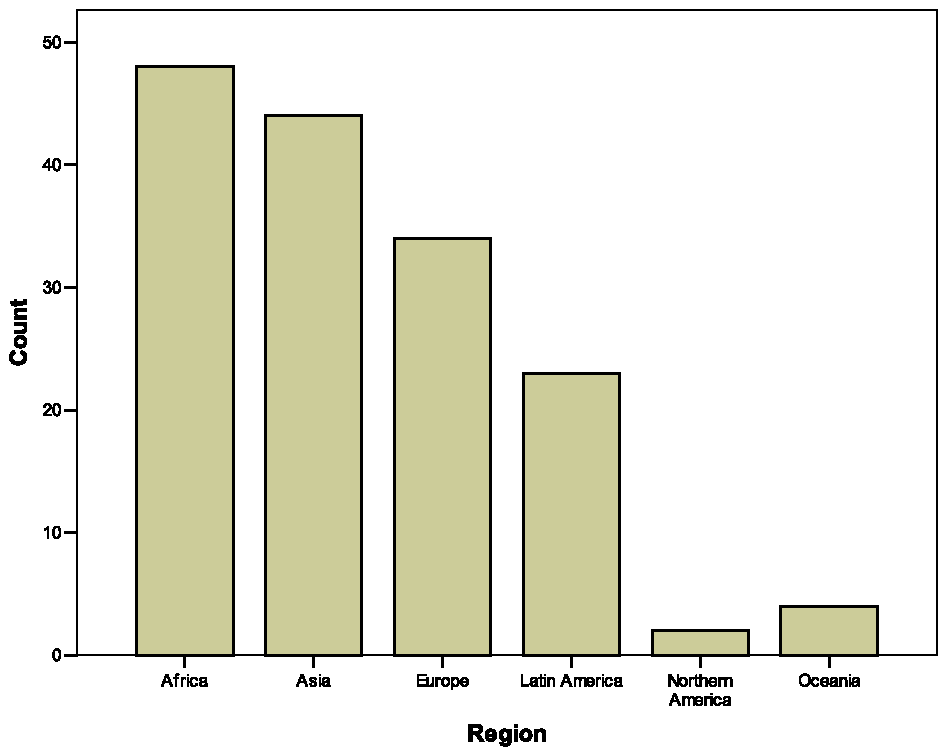
\includegraphics[height=9.50000cm]{regions.pdf}
\caption{\label{fig:f-bars-region} Bar chart of regions in the country
data.}
\end{figure}

\begin{figure}[htbp]
\centering
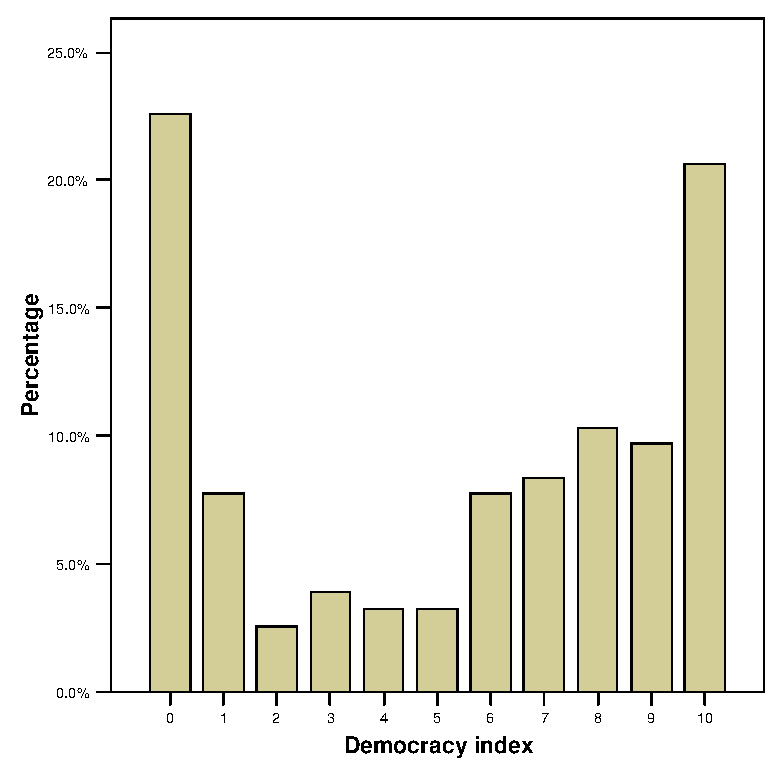
\includegraphics[height=9.50000cm]{democ.pdf}
\caption{\label{fig:f-bars-democ} Bar chart of the democracy index in the
country data.}
\end{figure}

\begin{figure}[htbp]
\centering
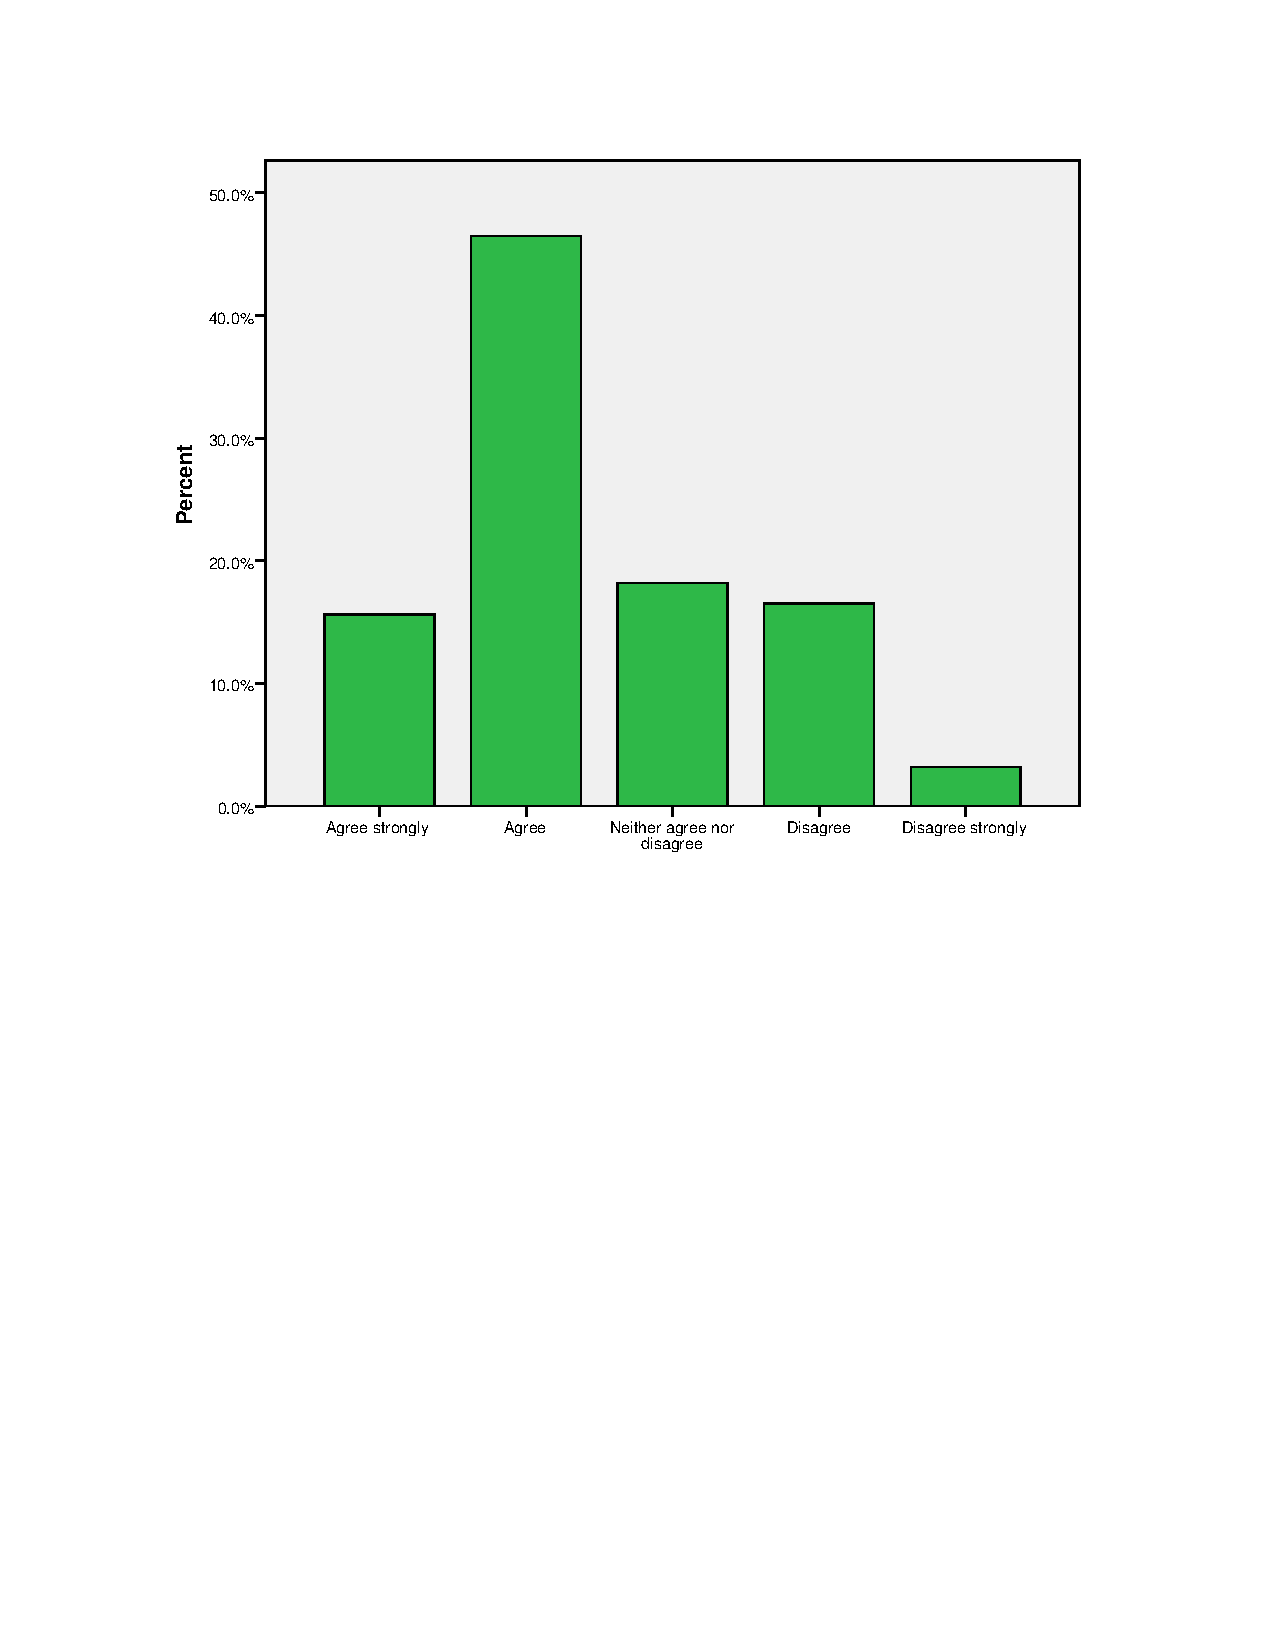
\includegraphics[height=8.00000cm]{bar_attitude.pdf}
\caption{\label{fig:f-bars-attitude} Bar chart of the attitude variable in
the survey data example. Agreement with statement: ``The government
should take measures to reduce differences in income levels''. European
Social Survey, Round 5 (2010), UK respondents only.}
\end{figure}

Some guidelines for drawing bar charts are:

\begin{itemize}
\item
  The heights of the bars may represent frequencies, proportions or
  percentages. This only changes the units on the vertical axis but not
  the relative heights of the bars. The shape of the graph will be the
  same in each case. In Figure \ref{fig:f-bars-region}, the units are
  frequencies, while in Figures \ref{fig:f-bars-democ} and
  \ref{fig:f-bars-attitude} they are percentages.
\item
  The bars do not touch each other, to highlight the discrete nature of
  the variable.
\item
  The bars \emph{must} start at zero. It they do not, visual comparisons
  between their heights are distorted and the graph becomes useless.
\item
  If the variable is ordinal, the bars must be in the natural order of
  the categories, as in Figures \ref{fig:f-bars-democ} and
  \ref{fig:f-bars-attitude}. If the variable is nominal, the order is
  arbitrary. Often it makes sense to order the categories from largest
  (i.e.~the one with the largest frequency) to the smallest, possibly
  leaving any ``Others'' category last. In Figure
  \ref{fig:f-bars-region}, the frequency ordering would swap Northern
  America and Oceania, but it seems more natural to keep Northern and
  Latin America next to each other.
\end{itemize}

A bar chart is a relatively unexciting statistical graphic in that it
does not convey very much visual information. For nominal variables, in
particular, the corresponding table is often just as easy to understand
and takes less space. For ordinal variables, the bar chart has the
additional advantage that its shape shows how the frequencies vary
across the ordering of the categories. For example, Figure
\ref{fig:f-bars-democ} quite effectively conveys the information that
the most common values of the democracy index are the extreme scores 0
and 10.

Sometimes you may see graphs which look like bar charts of this kind,
but which actually show the values of a single variable for some units
rather than frequncies or percentages. For example, a report on the
economies of East Asia might show a chart of GDP per capita for Japan,
China, South Korea and North Korea, with one bar for each country, and
their heights proportional to 28.2, 5.0, 17.8 and 1.3 respectively
(c.f.~the data in Table \ref{tab:t-countrydata}). The basic idea of such
graphs is the same as that of standard bar charts. However, they are not
particularly useful as descriptive statistics, since they simply display
values in the original data without any summarization or simplification.

\subsection{Simple descriptive
statistics}\label{ss-descr1-1cat-descriptives}

Instead of the whole sample distribution, we may want to summarise only
some individual aspects of it, such as its central tendency or
variation. Descriptive statistics that are used for this purpose are
broadly similar for both discrete and continuous variables, so they will
be discussed together for both in Section \ref{s-descr1-nums}.

\section{Two categorical variables}\label{s-descr1-2cat}

\subsection{Two-way contingency tables}\label{ss-descr1-2cat-tables}

The next task we consider is how to describe the sample distributions of
two categorical variables together, and in so doing also summarise the
association between these variables. The key tool is a table which shows
the \textbf{crosstabulation} of the frequencies of the variables. This
is also known as a \textbf{contingency table}. Table
\ref{tab:t-sex-attitude} shows such a table for the respondents' sex and
attitude in our survey example. We use it to introduce the basic
structure and terminology of contingency tables:

\begin{longtable}[]{@{}lcccccr@{}}
\caption{\label{tab:t-sex-attitude} \emph{``The government should take
measures to reduce differences in income levels''}: Two-way table of
frequencies of respondents in the survey example, by sex and attitude
towards income redistribution. Data: European Social Survey, Round 5,
2010, UK respondents only.}\tabularnewline
\toprule
\begin{minipage}[t]{0.21\columnwidth}\raggedright\strut
Sex\strut
\end{minipage} & \begin{minipage}[t]{0.13\columnwidth}\centering\strut
Agree strongly\strut
\end{minipage} & \begin{minipage}[t]{0.07\columnwidth}\centering\strut
Agree\strut
\end{minipage} & \begin{minipage}[t]{0.13\columnwidth}\centering\strut
Neither agree nor disagree\strut
\end{minipage} & \begin{minipage}[t]{0.09\columnwidth}\centering\strut
Disagree\strut
\end{minipage} & \begin{minipage}[t]{0.09\columnwidth}\centering\strut
Disagree strongly\strut
\end{minipage} & \begin{minipage}[t]{0.06\columnwidth}\raggedleft\strut
Total\strut
\end{minipage}\tabularnewline
\begin{minipage}[t]{0.21\columnwidth}\raggedright\strut
Male\strut
\end{minipage} & \begin{minipage}[t]{0.13\columnwidth}\centering\strut
160\strut
\end{minipage} & \begin{minipage}[t]{0.07\columnwidth}\centering\strut
439\strut
\end{minipage} & \begin{minipage}[t]{0.13\columnwidth}\centering\strut
187\strut
\end{minipage} & \begin{minipage}[t]{0.09\columnwidth}\centering\strut
200\strut
\end{minipage} & \begin{minipage}[t]{0.09\columnwidth}\centering\strut
41\strut
\end{minipage} & \begin{minipage}[t]{0.06\columnwidth}\raggedleft\strut
1027\strut
\end{minipage}\tabularnewline
\begin{minipage}[t]{0.21\columnwidth}\raggedright\strut
Female\strut
\end{minipage} & \begin{minipage}[t]{0.13\columnwidth}\centering\strut
206\strut
\end{minipage} & \begin{minipage}[t]{0.07\columnwidth}\centering\strut
651\strut
\end{minipage} & \begin{minipage}[t]{0.13\columnwidth}\centering\strut
239\strut
\end{minipage} & \begin{minipage}[t]{0.09\columnwidth}\centering\strut
187\strut
\end{minipage} & \begin{minipage}[t]{0.09\columnwidth}\centering\strut
34\strut
\end{minipage} & \begin{minipage}[t]{0.06\columnwidth}\raggedleft\strut
1317\strut
\end{minipage}\tabularnewline
\begin{minipage}[t]{0.21\columnwidth}\raggedright\strut
Total\strut
\end{minipage} & \begin{minipage}[t]{0.13\columnwidth}\centering\strut
366\strut
\end{minipage} & \begin{minipage}[t]{0.07\columnwidth}\centering\strut
1090\strut
\end{minipage} & \begin{minipage}[t]{0.13\columnwidth}\centering\strut
426\strut
\end{minipage} & \begin{minipage}[t]{0.09\columnwidth}\centering\strut
387\strut
\end{minipage} & \begin{minipage}[t]{0.09\columnwidth}\centering\strut
75\strut
\end{minipage} & \begin{minipage}[t]{0.06\columnwidth}\raggedleft\strut
2344\strut
\end{minipage}\tabularnewline
\bottomrule
\end{longtable}

\begin{itemize}
\item
  Because a table like \ref{tab:t-sex-attitude} summarizes the values of
  two variables, it is known as a \textbf{two-way} contingency table.
  Similarly, the tables of single variables introduced in Section
  \ref{ss-descr1-1cat-tables} are \emph{one-way} tables. It is also
  possible to construct tables involving more than two variables,
  i.e.~three-way tables, four-way tables, and so on. These are discussed
  in Chapter \ref{c-3waytables}.
\item
  The variables in a contingency table may ordinal or nominal (including
  dichotomous). Often an ordinal variable is derived by grouping an
  originally continuous, interval-level variable, a practice which is
  discussed further in Section \ref{s-descr1-1cont}.
\item
  The horizontal divisions of a table (e.g.~the lines corresponding to
  the two sexes in Table \ref{tab:t-sex-attitude}) are its
  \textbf{rows}, and the vertical divisions (e.g.~the survey responses
  in Table \ref{tab:t-sex-attitude}) are its \textbf{columns}.
\item
  The size of a contingency table is stated in terms of the numbers of
  its rows and columns. For example, Table \ref{tab:t-sex-attitude} is a
  \(2\times 5\) (pronounced ``two-by-five'') table, because it has two
  rows and five columns. This notation may also be used symbolically, so
  that we may refer generically to \(R\times C\) tables which have some
  (unspecified) number of \(R\) rows and \(C\) columns. The smallest
  two-way table is thus a \(2\times 2\) table, where both variables are
  dichotomous.
\item
  The intersection of a row and a column is a \textbf{cell} of the
  table. The basic two-way contingency table shows in each cell the
  number (frequency) of units in the data set with the corresponding
  values of the row variable and the column variable. For example, Table
  \ref{tab:t-sex-attitude} shows that there were 160 male respondents
  who strongly agreed with the statement, and 239 female respondents who
  neither agreed nor disagreed with it. These frequencies are also known
  as \textbf{cell counts}.
\item
  The row and column labelled ``Total'' in Table
  \ref{tab:t-sex-attitude} are known as the \textbf{margins} of the
  table. They show the frequencies of the values of the row and the
  column variable separately, summing the frequencies over the
  categories of the other variable. For example, the table shows that
  there were overall 1027 (\(=160+439+187+200+41\)) male respondents,
  and that overall 75 (\(=41+34\)) respondents strongly disagreed with
  the statement. In other words, the margins are \emph{one-way} tables
  of the frequencies of each of the two variables, so for example the
  frequencies on the margin for attitude in Table
  \ref{tab:t-sex-attitude} are the same as the ones in the one-way table
  for this variable shown in Table \ref{tab:t-attitude}. The
  distributions described by the margins are known as the
  \textbf{marginal distributions} of the row and column variables. In
  contrast, the frequencies in the internal cells of the table, which
  show how many units have each possible \emph{combination} of the row
  and column variables, describe the \textbf{joint distribution} of the
  two variables.
\item
  The number in the bottom right-hand corner of the table is the sum of
  all of the frequencies, i.e.~the total sample size \(n\).
\end{itemize}

In addition to frequencies, it is often convenient to display
proportions or percentages. Dividing the frequencies by the sample size
gives overall proportions and (multiplying by a hundred) percentages.
This is illustrated in Table \ref{tab:t-sex-attitude-pr}, which shows
the overall proportions, obtained by dividing the frequencies in Table
\ref{tab:t-sex-attitude} by \(n=2344\). For example, out of all these
respondents, the proportion of 0.102 (\(=239/2344\)) were women who
neither agreed nor disagreed with the statement. The proportions are
also shown for the marginal distributions: for example, 15.6\% (i.e.~the
proportion \(0.156=366/2344\)) of the respondents strongly agreed with
the statement. The sum of the proportions over all the cells is 1, as
shown in the bottom right corner of the table.

\begin{longtable}[]{@{}lcccccc@{}}
\caption{\label{tab:t-sex-attitude-pr} \emph{``The government should take
measures to reduce differences in income levels''}: Two-way table of
joint proportions of respondents in the survey example, with each
combination of sex and attitude towards income redistribution. Data:
European Social Survey, Round 5, 2010, UK respondents
only.}\tabularnewline
\toprule
\begin{minipage}[t]{0.14\columnwidth}\raggedright\strut
Sex\strut
\end{minipage} & \begin{minipage}[t]{0.15\columnwidth}\centering\strut
Agree strongly\strut
\end{minipage} & \begin{minipage}[t]{0.08\columnwidth}\centering\strut
Agree\strut
\end{minipage} & \begin{minipage}[t]{0.15\columnwidth}\centering\strut
Neither agree nor disagree\strut
\end{minipage} & \begin{minipage}[t]{0.10\columnwidth}\centering\strut
Disagree\strut
\end{minipage} & \begin{minipage}[t]{0.10\columnwidth}\centering\strut
Disagree strongly\strut
\end{minipage} & \begin{minipage}[t]{0.07\columnwidth}\centering\strut
Total\strut
\end{minipage}\tabularnewline
\begin{minipage}[t]{0.14\columnwidth}\raggedright\strut
Male\strut
\end{minipage} & \begin{minipage}[t]{0.15\columnwidth}\centering\strut
0.068\strut
\end{minipage} & \begin{minipage}[t]{0.08\columnwidth}\centering\strut
0.187\strut
\end{minipage} & \begin{minipage}[t]{0.15\columnwidth}\centering\strut
0.080\strut
\end{minipage} & \begin{minipage}[t]{0.10\columnwidth}\centering\strut
0.085\strut
\end{minipage} & \begin{minipage}[t]{0.10\columnwidth}\centering\strut
0.017\strut
\end{minipage} & \begin{minipage}[t]{0.07\columnwidth}\centering\strut
0.438\strut
\end{minipage}\tabularnewline
\begin{minipage}[t]{0.14\columnwidth}\raggedright\strut
Female\strut
\end{minipage} & \begin{minipage}[t]{0.15\columnwidth}\centering\strut
0.088\strut
\end{minipage} & \begin{minipage}[t]{0.08\columnwidth}\centering\strut
0.278\strut
\end{minipage} & \begin{minipage}[t]{0.15\columnwidth}\centering\strut
0.102\strut
\end{minipage} & \begin{minipage}[t]{0.10\columnwidth}\centering\strut
0.080\strut
\end{minipage} & \begin{minipage}[t]{0.10\columnwidth}\centering\strut
0.015\strut
\end{minipage} & \begin{minipage}[t]{0.07\columnwidth}\centering\strut
0.562\strut
\end{minipage}\tabularnewline
\begin{minipage}[t]{0.14\columnwidth}\raggedright\strut
Total\strut
\end{minipage} & \begin{minipage}[t]{0.15\columnwidth}\centering\strut
0.156\strut
\end{minipage} & \begin{minipage}[t]{0.08\columnwidth}\centering\strut
0.465\strut
\end{minipage} & \begin{minipage}[t]{0.15\columnwidth}\centering\strut
0.182\strut
\end{minipage} & \begin{minipage}[t]{0.10\columnwidth}\centering\strut
0.165\strut
\end{minipage} & \begin{minipage}[t]{0.10\columnwidth}\centering\strut
0.032\strut
\end{minipage} & \begin{minipage}[t]{0.07\columnwidth}\centering\strut
1.000\strut
\end{minipage}\tabularnewline
\bottomrule
\end{longtable}

\subsection{Conditional proportions}\label{ss-descr1-2cat-cond}

A two-way contingency table is symmetric in that it does not distinguish
between explanatory and response variables. In many applications,
however, this distinction is useful for interpretation. In our example,
for instance, it is natural to treat sex as the explanatory variable and
attitude towards income redistribution as the response response, and so
to focus the interpretation on how attitude may depend on sex.

The overall proportions are in such cases not the most relevant
quantities for interpretation of a table. Instead, we typically
calculate proportions within each category of the row variable or the
column variable, i.e.~the \textbf{conditional proportions} of one
variable given the other. The numbers in brackets in Table
\ref{tab:t-sex-attitude-row} show these proportions calculated for each
\emph{row} of Table \ref{tab:t-sex-attitude} (Table
\ref{tab:t-sex-attitude-row} also includes the actual frequencies; it is
advisable to include them even when conditional proportions are of most
interest, to show the numbers on which the proportions are based). In
other words, these are the conditional proportions of attitude towards
income redistribution given sex, i.e.~separately for men and women. For
example, the number 0.156 in the top left-hand corner of Table
\ref{tab:t-sex-attitude-row} is obtained by dividing the number of male
respondents who agreed strongly with the statement (160) by the total
number of male respondents (1027). Thus 15.6\% of the men strongly
agreed, and for example 2.6\% of women strongly disagreed with the
statement. The (1.0) in the last column of the table indicate that the
proportions sum to 1 along each row, to remind us that the conditional
proportions have been calculated within the rows. The bracketed
proportions in the `Total' row are the proportions of the
\emph{marginal} distribution of the attitude variable, so they are the
same as the proportions in the `Total' row of Table
\ref{tab:t-sex-attitude-pr}.

\begin{longtable}[]{@{}lcccccc@{}}
\caption{\label{tab:t-sex-attitude-row} \emph{``The government should take
measures to reduce differences in income levels''}: Two-way table of
frequencies of respondents in the survey example, by sex and attitude
towards income redistribution. The numbers in brackets are proportions
within the rows, i.e.~conditional proportions of attitude given sex.
Data: European Social Survey, Round 5, 2010, UK respondents
only.}\tabularnewline
\toprule
\begin{minipage}[t]{0.13\columnwidth}\raggedright\strut
Sex\strut
\end{minipage} & \begin{minipage}[t]{0.15\columnwidth}\centering\strut
Agree strongly\strut
\end{minipage} & \begin{minipage}[t]{0.09\columnwidth}\centering\strut
Agree\strut
\end{minipage} & \begin{minipage}[t]{0.15\columnwidth}\centering\strut
Neither agree nor disagree\strut
\end{minipage} & \begin{minipage}[t]{0.10\columnwidth}\centering\strut
Disagree\strut
\end{minipage} & \begin{minipage}[t]{0.10\columnwidth}\centering\strut
Disagree strongly\strut
\end{minipage} & \begin{minipage}[t]{0.07\columnwidth}\centering\strut
Total\strut
\end{minipage}\tabularnewline
\begin{minipage}[t]{0.13\columnwidth}\raggedright\strut
Male\strut
\end{minipage} & \begin{minipage}[t]{0.15\columnwidth}\centering\strut
160\strut
\end{minipage} & \begin{minipage}[t]{0.09\columnwidth}\centering\strut
439\strut
\end{minipage} & \begin{minipage}[t]{0.15\columnwidth}\centering\strut
187\strut
\end{minipage} & \begin{minipage}[t]{0.10\columnwidth}\centering\strut
200\strut
\end{minipage} & \begin{minipage}[t]{0.10\columnwidth}\centering\strut
41\strut
\end{minipage} & \begin{minipage}[t]{0.07\columnwidth}\centering\strut
1027\strut
\end{minipage}\tabularnewline
\begin{minipage}[t]{0.13\columnwidth}\raggedright\strut
\strut
\end{minipage} & \begin{minipage}[t]{0.15\columnwidth}\centering\strut
(0.156)\strut
\end{minipage} & \begin{minipage}[t]{0.09\columnwidth}\centering\strut
(0.428)\strut
\end{minipage} & \begin{minipage}[t]{0.15\columnwidth}\centering\strut
(0.182)\strut
\end{minipage} & \begin{minipage}[t]{0.10\columnwidth}\centering\strut
(0.195)\strut
\end{minipage} & \begin{minipage}[t]{0.10\columnwidth}\centering\strut
(0.040)\strut
\end{minipage} & \begin{minipage}[t]{0.07\columnwidth}\centering\strut
(1.0)\strut
\end{minipage}\tabularnewline
\begin{minipage}[t]{0.13\columnwidth}\raggedright\strut
Female\strut
\end{minipage} & \begin{minipage}[t]{0.15\columnwidth}\centering\strut
206\strut
\end{minipage} & \begin{minipage}[t]{0.09\columnwidth}\centering\strut
651\strut
\end{minipage} & \begin{minipage}[t]{0.15\columnwidth}\centering\strut
239\strut
\end{minipage} & \begin{minipage}[t]{0.10\columnwidth}\centering\strut
187\strut
\end{minipage} & \begin{minipage}[t]{0.10\columnwidth}\centering\strut
34\strut
\end{minipage} & \begin{minipage}[t]{0.07\columnwidth}\centering\strut
1317\strut
\end{minipage}\tabularnewline
\begin{minipage}[t]{0.13\columnwidth}\raggedright\strut
\strut
\end{minipage} & \begin{minipage}[t]{0.15\columnwidth}\centering\strut
(0.156)\strut
\end{minipage} & \begin{minipage}[t]{0.09\columnwidth}\centering\strut
(0.494)\strut
\end{minipage} & \begin{minipage}[t]{0.15\columnwidth}\centering\strut
(0.182)\strut
\end{minipage} & \begin{minipage}[t]{0.10\columnwidth}\centering\strut
(0.142)\strut
\end{minipage} & \begin{minipage}[t]{0.10\columnwidth}\centering\strut
(0.026)\strut
\end{minipage} & \begin{minipage}[t]{0.07\columnwidth}\centering\strut
(1.0)\strut
\end{minipage}\tabularnewline
\begin{minipage}[t]{0.13\columnwidth}\raggedright\strut
Total\strut
\end{minipage} & \begin{minipage}[t]{0.15\columnwidth}\centering\strut
366\strut
\end{minipage} & \begin{minipage}[t]{0.09\columnwidth}\centering\strut
1090\strut
\end{minipage} & \begin{minipage}[t]{0.15\columnwidth}\centering\strut
426\strut
\end{minipage} & \begin{minipage}[t]{0.10\columnwidth}\centering\strut
387\strut
\end{minipage} & \begin{minipage}[t]{0.10\columnwidth}\centering\strut
75\strut
\end{minipage} & \begin{minipage}[t]{0.07\columnwidth}\centering\strut
2344\strut
\end{minipage}\tabularnewline
\begin{minipage}[t]{0.13\columnwidth}\raggedright\strut
\strut
\end{minipage} & \begin{minipage}[t]{0.15\columnwidth}\centering\strut
(0.156)\strut
\end{minipage} & \begin{minipage}[t]{0.09\columnwidth}\centering\strut
(0.465)\strut
\end{minipage} & \begin{minipage}[t]{0.15\columnwidth}\centering\strut
(0.182)\strut
\end{minipage} & \begin{minipage}[t]{0.10\columnwidth}\centering\strut
(0.165)\strut
\end{minipage} & \begin{minipage}[t]{0.10\columnwidth}\centering\strut
(0.032)\strut
\end{minipage} & \begin{minipage}[t]{0.07\columnwidth}\centering\strut
(1.0)\strut
\end{minipage}\tabularnewline
\bottomrule
\end{longtable}

We could also have calculated conditional proportions within the
\emph{columns}, i.e.~for sex given attitude. For example, the proportion
\(0.563=206/366\) of all respondents who strongly agreed with the
statement are women. These, however, seem less interesting, because it
seems more natural to examine how attitude varies by sex rather than how
sex varies by attitude. In general, for any two-way table we can
calculate conditional proportions for both the rows and the columns, but
typically only one of them is used for interpretation.

\subsection{Conditional distributions and
associations}\label{ss-descr1-2cat-assoc}

Suppose that we regard one variable in a two-way table as the
explanatory variable (let us denote it by \(X\)) and the other variable
as the response variable (\(Y\)). In our survey example, sex is thus
\(X\) and attitude is \(Y\). Here the dichotomous \(X\) divides the full
sample into two groups, identified by the observed value of \(X\) ---
men and women. We may then think of these two groups as two separate
samples, and consider statistical quantities separately for each of
them. In particular, in Table \ref{tab:t-sex-attitude-row} we calculated
conditional proportions for \(Y\) given \(X\), i.e.~for attitude given
sex. These proportions describe two distinct sample distributions of
\(Y\), one for men and one for women. They are examples of
\emph{conditional distributions}:

\begin{itemize}
\tightlist
\item
  The \textbf{conditional distribution} of a variable \(Y\) given
  another variable \(X\) is the distribution of \(Y\) among those units
  which have a particular value of \(X\).
\end{itemize}

This concept is not limited to two-way tables but extends also to other
kinds of variables and distributions that are discussed later in this
coursepack. Both the response variable \(Y\) and the explanatory
variable \(X\) may be continuous as well as discrete, and can have any
number of values. In all such cases there is a separate conditional
distribution for \(Y\) for each possible value of \(X\). A particular
one of these distributions is sometimes referred to more explicitly as
the conditional distribution of \(Y\) given \(X=x\), where the
``\(X=x\)'' indicates that \(X\) is considered at a particular value
\(x\) (as in ``the distribution of \(Y\) given \(X=2\)'', say).

Conditional distributions of one variable given another allow us to
define and describe associations between the variables. The informal
definition in Section \ref{ss-intro-def-assoc} stated that there is an
association between two variables if knowing the value of one of them
will help to predict the value of the other. We can now give a more
precise definition:

\begin{itemize}
\tightlist
\item
  There is an \textbf{association} between variables \(X\) and \(Y\) if
  the conditional distribution of \(Y\) given \(X\) is different for
  different values of \(X\).
\end{itemize}

This definition coincides with the more informal one. If the conditional
distribution of \(Y\) varies with \(X\) and if we know \(X\), it is best
to predict \(Y\) from its conditional distribution given the known value
of \(X\). This will indeed work better than predicting \(Y\) without
using information on \(X\), i.e.~from the marginal distribution of
\(Y\). Prediction based on the conditional distribution would still be
subject to error, because in most cases \(X\) does not predict \(Y\)
perfectly. In other words, the definition of an association considered
here is \emph{statistical} (or \emph{probabilistic}) rather than
\emph{deterministic}. In our example a deterministic association would
mean that there is one response given by all the men and one response
(possibly different from the men's) given by all the women. This is of
course not the case here nor in most other applications in the social
sciences. It is thus crucially important that we have the tools also to
analyse statistical associations.

In our example, sex and attitude are associated if men and women differ
in their attitudes toward income redistribution. Previous studies
suggest that such an association exists, and that it takes the form that
women tend to have higher levels of support than men for
redistribution.\footnote{The data can be obtained from
  \texttt{http://www3.norc.org/gss+website/}, which gives further
  information on the survey, including the full text of the
  questionnaires.} As possible explanations for this pattern, both
structural reasons (women tend to have lower incomes than men and to
rely more on welfare state support) and cultural or psychological ones
(women are more likely than men to adopt social values of equality and
caring) have been suggested.

\subsection{Describing an association using conditional
proportions}\label{ss-descr1-2cat-descr}

Two variables presented in a contingency table are associated in the
sample if the conditional distributions of one of them vary across the
values of the other. This is the case in our data set: for example,
4.0\% of men but 2.6\% of women strongly disagree with the statement.
There is thus some association between sex and attitude in this sample.
This much is easy to conclude. What requires a little more work is a
more detailed description of the pattern and strength of the
association, i.e.~how and where the conditional distributions differ
from each other.

The most general way of summarising associations in a contingency table
is by comparing the conditional proportions of the same level of the
response given different levels of the explanatory variable. There is no
simple formula for how this should be done, so you should use your
common sense to present comparisons which give a good summary of the
patterns across the table. Unless both variables in the table are
dichotomous, several different comparisons may be needed, and may not
all display similar patterns. For example, in Table
\ref{tab:t-sex-attitude-row} the same proportion (0.156, or 15.6\%) of
both men and women strongly agree with the statement, whereas the
proportion who respond ``Agree'' is higher for women (49.4\%) than for
men (42.8\%).

When the response variable is ordinal, it is often more illuminating to
focus on comparisons of \emph{cumulative} proportions which add up
conditional proportions over two or more adjacent categories. For
instance, the combined proportion of respondents who either strongly
agree or agree with the statement is a useful summary of the general
level of agreement among the respondents. In our example this is 58.4\%
(\(=15.5\%+42.8\%\)) for men but 65.0\% for women.

A comparison between two proportions may be further distilled into a
single number by reporting the \emph{difference} or \emph{ratio} between
them. For example, for the proportions of agreeing or strongly agreeing
above, the difference is \(0.650-0.584=0.066\), so the proportion is
0.066 (i.e.~6.6 percentage points) higher for women than for men. The
ratio of these proportions is \(0.650/0.584=1.11\), so the proportion
for women is 1.11 times the proportion for men (i.e.~11\% higher). Both
of these indicate that in this sample women were more likely to agree or
strongly agree with the statement than were men. In a particular
application we might report a difference or a ratio like this, depending
on which of them was considered more relevant or easily understandable.
Other summaries are also possible; for example, on MY452 we will discuss
a measure called the \emph{odds ratio}, which turns out to be convenient
for more general methods of analysing associations involving categorical
variables.

The broad conclusion in the example is that there is an association
between sex and attitude in these data from the European Social Survey,
and that it is of the kind suggested by existing literature. A larger
proportion of women than of men indicate agreement with the statement
that the government should take measures to reduce income differences,
and conversely larger proportion of men disagree with it (e.g.~23.5\% of
men but only 16.8\% of women disagree or strongly disagree). Thus in
this sample women do indeed demonstrate somewhat higher levels of
support for income redistribution. Whether these differences also
warrant a generalisation of the conclusions to people outside the sample
is a question which we will take up in Chapters \ref{c-samples} and
\ref{c-tables}.

\subsection{A measure of association for ordinal
variables}\label{ss-descr1-2cat-gamma}

In the previous example the explanatory variable (sex) had 2 categories
and the response variable (attitude) had 5. A full examination of the
individual conditional distributions of attitude given sex then involved
comparisons of five pairs of proportions, one for each level of the
attitude variable. This number gets larger still if the explanatory
variable also has several levels, as in the following example:

\emph{Example: Importance of short-term gains for investors}

Information on the behaviour and expectations of individual investors
was collected by sending a questionnaire to a sample of customers of a
U.S.~brokerage house.\footnote{ESS Round 5: European Social Survey Round
  5 Data (2010). Data file edition 2.0. Norwegian Social Science Data
  Services, Norway � Data Archive and distributor of ESS data. The full
  data can be obtained from \texttt{http://ess.nsd.uib.no/ess/round5/}.}
One of the questions asked the respondents to state how much importance
they placed on quick profits (short-term gains) as an objective when
they invested money. The responses were recorded in four categories as
``Irrelevant'', ``Slightly important'', ``Important'' or ``Very
important''. Table \ref{tab:t-investors} shows the crosstabulation of
this variable with the age of the respondent in four age groups.

\begin{longtable}[]{@{}lrrrrr@{}}
\caption{\label{tab:t-investors} Importance of short-term gains: Frequencies
of respondents in the investment example, by age group and attitude
towards short-term gains as investment goal. Conditional proportions of
attitude given age group are shown in brackets. The value of the
\(\gamma\) measure of association is \(-0.377\).}\tabularnewline
\toprule
\begin{minipage}[t]{0.10\columnwidth}\raggedright\strut
Age group\strut
\end{minipage} & \begin{minipage}[t]{0.40\columnwidth}\raggedleft\strut
Irrelevant\strut
\end{minipage} & \begin{minipage}[t]{0.09\columnwidth}\raggedleft\strut
Slightly important\strut
\end{minipage} & \begin{minipage}[t]{0.09\columnwidth}\raggedleft\strut
Important\strut
\end{minipage} & \begin{minipage}[t]{0.09\columnwidth}\raggedleft\strut
Very important\strut
\end{minipage} & \begin{minipage}[t]{0.06\columnwidth}\raggedleft\strut
Total\strut
\end{minipage}\tabularnewline
\begin{minipage}[t]{0.10\columnwidth}\raggedright\strut
Under 45\strut
\end{minipage} & \begin{minipage}[t]{0.40\columnwidth}\raggedleft\strut
37\strut
\end{minipage} & \begin{minipage}[t]{0.09\columnwidth}\raggedleft\strut
45\strut
\end{minipage} & \begin{minipage}[t]{0.09\columnwidth}\raggedleft\strut
38\strut
\end{minipage} & \begin{minipage}[t]{0.09\columnwidth}\raggedleft\strut
26\strut
\end{minipage} & \begin{minipage}[t]{0.06\columnwidth}\raggedleft\strut
146\strut
\end{minipage}\tabularnewline
\begin{minipage}[t]{0.10\columnwidth}\raggedright\strut
\strut
\end{minipage} & \begin{minipage}[t]{0.40\columnwidth}\raggedleft\strut
(0.253)\strut
\end{minipage} & \begin{minipage}[t]{0.09\columnwidth}\raggedleft\strut
(0.308)\strut
\end{minipage} & \begin{minipage}[t]{0.09\columnwidth}\raggedleft\strut
(0.260)\strut
\end{minipage} & \begin{minipage}[t]{0.09\columnwidth}\raggedleft\strut
(0.178)\strut
\end{minipage} & \begin{minipage}[t]{0.06\columnwidth}\raggedleft\strut
(1.00)\strut
\end{minipage}\tabularnewline
\begin{minipage}[t]{0.10\columnwidth}\raggedright\strut
45--54\strut
\end{minipage} & \begin{minipage}[t]{0.40\columnwidth}\raggedleft\strut
111\strut
\end{minipage} & \begin{minipage}[t]{0.09\columnwidth}\raggedleft\strut
77\strut
\end{minipage} & \begin{minipage}[t]{0.09\columnwidth}\raggedleft\strut
57\strut
\end{minipage} & \begin{minipage}[t]{0.09\columnwidth}\raggedleft\strut
37\strut
\end{minipage} & \begin{minipage}[t]{0.06\columnwidth}\raggedleft\strut
282\strut
\end{minipage}\tabularnewline
\begin{minipage}[t]{0.10\columnwidth}\raggedright\strut
\strut
\end{minipage} & \begin{minipage}[t]{0.40\columnwidth}\raggedleft\strut
(0.394)\strut
\end{minipage} & \begin{minipage}[t]{0.09\columnwidth}\raggedleft\strut
(0.273)\strut
\end{minipage} & \begin{minipage}[t]{0.09\columnwidth}\raggedleft\strut
(0.202)\strut
\end{minipage} & \begin{minipage}[t]{0.09\columnwidth}\raggedleft\strut
(0.131)\strut
\end{minipage} & \begin{minipage}[t]{0.06\columnwidth}\raggedleft\strut
(1.00)\strut
\end{minipage}\tabularnewline
\begin{minipage}[t]{0.10\columnwidth}\raggedright\strut
55--64\strut
\end{minipage} & \begin{minipage}[t]{0.40\columnwidth}\raggedleft\strut
153\strut
\end{minipage} & \begin{minipage}[t]{0.09\columnwidth}\raggedleft\strut
49\strut
\end{minipage} & \begin{minipage}[t]{0.09\columnwidth}\raggedleft\strut
31\strut
\end{minipage} & \begin{minipage}[t]{0.09\columnwidth}\raggedleft\strut
20\strut
\end{minipage} & \begin{minipage}[t]{0.06\columnwidth}\raggedleft\strut
253\strut
\end{minipage}\tabularnewline
\begin{minipage}[t]{0.10\columnwidth}\raggedright\strut
\strut
\end{minipage} & \begin{minipage}[t]{0.40\columnwidth}\raggedleft\strut
(0.605)\strut
\end{minipage} & \begin{minipage}[t]{0.09\columnwidth}\raggedleft\strut
(0.194)\strut
\end{minipage} & \begin{minipage}[t]{0.09\columnwidth}\raggedleft\strut
(0.123)\strut
\end{minipage} & \begin{minipage}[t]{0.09\columnwidth}\raggedleft\strut
(0.079)\strut
\end{minipage} & \begin{minipage}[t]{0.06\columnwidth}\raggedleft\strut
(1.00)\strut
\end{minipage}\tabularnewline
\begin{minipage}[t]{0.10\columnwidth}\raggedright\strut
65 and over\strut
\end{minipage} & \begin{minipage}[t]{0.40\columnwidth}\raggedleft\strut
193\strut
\end{minipage} & \begin{minipage}[t]{0.09\columnwidth}\raggedleft\strut
64\strut
\end{minipage} & \begin{minipage}[t]{0.09\columnwidth}\raggedleft\strut
19\strut
\end{minipage} & \begin{minipage}[t]{0.09\columnwidth}\raggedleft\strut
15\strut
\end{minipage} & \begin{minipage}[t]{0.06\columnwidth}\raggedleft\strut
291\strut
\end{minipage}\tabularnewline
\begin{minipage}[t]{0.10\columnwidth}\raggedright\strut
\strut
\end{minipage} & \begin{minipage}[t]{0.40\columnwidth}\raggedleft\strut
(0.663)\strut
\end{minipage} & \begin{minipage}[t]{0.09\columnwidth}\raggedleft\strut
(0.220)\strut
\end{minipage} & \begin{minipage}[t]{0.09\columnwidth}\raggedleft\strut
(0.065)\strut
\end{minipage} & \begin{minipage}[t]{0.09\columnwidth}\raggedleft\strut
(0.052)\strut
\end{minipage} & \begin{minipage}[t]{0.06\columnwidth}\raggedleft\strut
(1.00)\strut
\end{minipage}\tabularnewline
\begin{minipage}[t]{0.10\columnwidth}\raggedright\strut
Total\strut
\end{minipage} & \begin{minipage}[t]{0.40\columnwidth}\raggedleft\strut
494\strut
\end{minipage} & \begin{minipage}[t]{0.09\columnwidth}\raggedleft\strut
235\strut
\end{minipage} & \begin{minipage}[t]{0.09\columnwidth}\raggedleft\strut
145\strut
\end{minipage} & \begin{minipage}[t]{0.09\columnwidth}\raggedleft\strut
98\strut
\end{minipage} & \begin{minipage}[t]{0.06\columnwidth}\raggedleft\strut
972\strut
\end{minipage}\tabularnewline
\bottomrule
\end{longtable}

Here there are four conditional distributions, one for each age group,
and each of them is described by four proportions of different levels of
attitude. There are then many possible comparisons of the kind discussed
above. For example, we might want to compare the proportions of
respondents who consider short-term gains irrelevant between the oldest
and the youngest age group, the proportions for whom such gains are very
important between these two groups, or, in general, the proportions in
any category of the response variable between any two age groups.

Although pairwise comparisons like this are important and informative,
they can clearly become cumbersome when the number of possible
comparisons is large. A potentially attractive alternative is then to
try to summarise the strength of the association between the variables
in a single number, a \textbf{measure of association} of some kind.
There are many such measures for two-way contingency tables, labelled
with a range of Greek and Roman letters (e.g. \(\phi\), \(\lambda\),
\(\gamma\), \(\rho\), \(\tau\), V, Q, U and d). The most useful of them
are designed for tables where both of the variables are measured at the
ordinal level, as is the case in Table \ref{tab:t-investors}. The
ordering of the categories can then be exploited to capture the strength
of the association in a single measure. This is not possible when at
least one of the variables is measured at the nominal level, as any
attempt to reduce the patterns of the conditional probabilities into one
number will then inevitably obscure much of the information in the
table. It is better to avoid measures of association defined for nominal
variables, and to describe their associations only through comparisons
of conditional probabilities as described in the previous section.

Here we will discuss only one measure of association for two-way tables
of ordinal variables. It is known as \(\gamma\) (``gamma''). It
characterises one possible general pattern of association between two
ordinal variables, namely the extent to which high values of one
variable tend to be associated with high or low values of the other
variable. Here speaking of ``low'' and ``high'' values, or of
``increasing'' or ``decreasing'' them, is meaningful when the variables
are ordinal. For example, in Table \ref{tab:t-investors} the categories
corresponding to the bottom rows and right-most columns are in an
obvious sense ``high'' values of age and importance respectively.

Consider the conditional proportions of importance given age group shown
in Table \ref{tab:t-investors}. It is clear that, for example, the
proportion of respondents for whom short-term gains are very important
is highest in the youngest, and lowest in the oldest age group.
Similarly, the proportion of respondents for whom such gains are
irrelevant increases consistently from the youngest to the oldest group.
In other words, respondents with \emph{high} values of the explanatory
variable (age group) tend to have \emph{low} values the response
variable (importance of short-term gains). Such an association is said
to be \emph{negative}. A \emph{positive} association would be seen in a
table where high values of one variable were associated with high values
of the other.

Measures of association for summarising such patterns are typically
based on the numbers of concordant and discordant pairs of observations.
Suppose we compare two units classified according to the two variables
in the table. These units form a \emph{concordant pair} if one of them
has a higher value of both variables than the other. For example,
consider two respondents in Table \ref{tab:t-investors}, one with values
(Under 45; Irrelevant) and the other with (45--54; Important). This is a
concordant pair, because the second respondent has both a higher value
of age group (45--54 vs.~Under 45) and a higher value of the importance
variable (Important vs.~Irrelevant) than the first respondent. In
contrast, in a \emph{discordant pair} one unit has a higher value of one
variable but a lower value of the other variable than the other unit.
For example, a pair of respondents with values (45--54; Very important)
and (55--64; Irrelevant) is discordant, because the latter has a higher
value of age group but a lower value of the importance variable than the
former. Pairs of units with the same value of one or both of the
variables are known as \emph{tied} pairs. They are not used in the
calculations discussed below.

The \(\gamma\) measure of association is defined as

\begin{equation}\gamma=\frac{C-D}{C+D}
\label{eq:gamma}\end{equation}

where \(C\) is the total number of concordant pairs in the table, and
\(D\) is the number of discordant pairs. For Table
\ref{tab:t-investors}, the value of this is \(\gamma=-0.377\).

Calculation of \(C\) and \(D\) is straightforward but tedious and
uninteresting, and can be left to a computer. Remembering the exact form
of (\ref{eq:gamma}) is also not crucial. More important than the formula
of \(\gamma\) (or any other measure of association) is its
interpretation. This can be considered on several levels of specificity,
which are discussed separately below. The discussion is relatively
detailed, as these considerations are relevant and useful not only for
\(\gamma\), but also for all other measures of association in
statistics.

The \textbf{sign} of the statistic: It can be seen from (\ref{eq:gamma})
that \(\gamma\) is positive (greater than zero) when there are more
concordant pairs than discordant ones (i.e.~\(C>D\)), and negative when
there are more discordant than concordant pairs (\(C<D\)). This also
implies that \(\gamma\) will be positive when the association is
positive in the sense discussed above, and negative when the association
is negative. A value of \(\gamma=0\) indicates a complete lack of
association of this kind. In Table \ref{tab:t-investors} we have
\(\gamma=-0.377\), indicating a negative association. This agrees with
the conclusion obtained informally above.

The \textbf{extreme values} of the statistic: Clearly \(\gamma=1\) if
there are no discordant pairs (\(D=0\)), and \(\gamma=-1\) if there are
no concordant pairs (\(C=0\)). The values \(\gamma=-1\) and \(\gamma=1\)
are the smallest and largest possible values of \(\gamma\), and indicate
the strongest possible levels of negative and positive association
respectively. More generally, the closer \(\gamma\) is to \(-1\) or 1,
the stronger is the (negative or positive) association.

The \textbf{formal interpretation} of the statistic: This refers to any
way of interpreting the value more understandably than just vaguely as a
measure of ``strength of association''. Most often, such an
intepretation is expressed as a \emph{proportion} of some kind. For
\(\gamma\), this is done using a principle known as \textbf{Proportional
reduction of error} (PRE). Because the PRE idea is also used to
interpret many other measures of association in statistics, we will
first describe it in general terms which are not limited to \(\gamma\).

Suppose we consider an explanatory variable \(X\) and a response
variable \(Y\), and want to make predictions of the values of \(Y\) in a
data set. This is done twice, first in a way which makes no use of
\(X\), and then in a way which predicts the value of \(Y\) for each unit
using information on the corresponding value of \(X\) and on the
strength and direction of the association between \(X\) and \(Y\).
Recalling the connection between association and prediction, it is clear
that the second approach should result in better predictions if the two
variables are associated. The comparison also reflects the
\emph{strength} of the association: the stronger it is, the bigger is
the improvement in prediction gained by utilising information on \(X\).

A PRE measure describes the size of this improvement. Suppose that the
magnitude or number of errors made in predicting the values of \(Y\) in
a data set using the first scheme, i.e.~ignoring information on \(X\),
is somehow measured by a single number \(E_{1}\), and that \(E_{2}\) is
the same measure of errors for the second prediction scheme which makes
use of \(X\). The difference \(E_{1}-E_{2}\) is thus the improvement in
prediction achieved by the second scheme over the first. A PRE measure
of association is the ratio

\begin{equation}\text{PRE}= \frac{E_{1}-E_{2}}{E_{1}},
\label{eq:PRE}\end{equation}

i.e.~the improvement in predictions as a \emph{proportion} of the number
of errors \(E_{1}\) under the first scheme. This formulation is
convenient for interpretation, because a proportion is easily
understandable even if \(E_{1}\) and \(E_{2}\) themselves are expressed
in some unfamiliar units. The smallest possible value of (\ref{eq:PRE})
is clearly 0, obtained when \(E_{2}=E_{1}\), i.e.~when using information
on \(X\) gives no improvement in predictions. The largest possible value
of PRE is 1, obtained when \(E_{2}=0\), i.e.~when \(Y\) can be predicted
perfectly from \(X\). The values 0 and 1 indicate no association and
perfect association respectively.

The \(\gamma\) statistic is a PRE measure, although with a somewhat
convoluted explanation. Suppose that we consider a pair of observations
which is known to be either concordant or discordant (the PRE
interpretation of \(\gamma\) ignores tied observations). One of the two
observations thus has a higher value of \(X\) than the other. For
example, suppose that we consider two respondents in Table
\ref{tab:t-investors} from different age groups. We are then asked to
predict the \emph{order} of the values of \(Y\), i.e.~which of the two
units has the higher value of \(Y\). In the example of Table
\ref{tab:t-investors}, this means predicting whether the older
respondent places a higher or lower level of importance on short-term
gains than the younger respondent. Two sets of predictions are again
compared. The first approach makes the prediction at random and with
equal probabilities, essentially tossing a coin to guess whether the
observation with the higher value of \(X\) has the higher or lower value
of \(Y\). The second prediction makes use of information on the
direction of the association between \(X\) and \(Y\). If the association
is known to be negative (i.e.~there are more discordant than concordant
pairs), every pair is predicted to be discordant; if it is positive,
every pair is predicted to be concordant. For example, in Table
\ref{tab:t-investors} the association is negative, so we would always
predict that the older of two respondents places a lower value of
importance on short-term gains.

If these predictions are repeated for every non-tied pair in the table,
the expected number of incorrect predictions under the first scheme is
\(E_{1}=(C+D)/2\). Under the second scheme it is \(E_{2}=D\) if the
association is positive and \(E_{2}=C\) if it is negative. Substituting
these into the general formula (\ref{eq:PRE}) shows that the \(\gamma\)
statistic (\ref{eq:gamma}) is of the PRE form when \(\gamma\) is
positive; when it is negative, the absolute value of \(\gamma\)
(i.e.~its value with the minus sign omitted) is a PRE measure, and the
negative sign of \(\gamma\) indicates that the association is in the
negative direction. In our example \(\gamma=-0.377\), so age and
attitude are negatively associated. Its absolute value \(0.377\) shows
that we will make 37.7\% fewer errors if we predict for every non-tied
pair that the older respondent places less importance on short-term
gains, compared to predictions made by tossing a coin for each pair.

The final property of interest is the \textbf{substantive
interpretation} of the strength of association indicated by \(\gamma\)
for a particular table. For example, should \(\gamma=-0.377\) for Table
\ref{tab:t-investors} be regarded as evidence of weak, moderate or
strong negative association between age and attitude? Although this is
usually the most (or only) interesting part of the interpretation, it is
also the most difficult, and one to which a statistician's response is
likely to be a firm ``it depends''. This is because the strength of
associations we may expect to observe depends on the variables under
consideration: a \(\gamma\) of 0.5, say, might be commonplace for some
types of variables but never observed for others. Considerations of the
magnitude of \(\gamma\) are most useful in comparisons of associations
between the same two variables in different samples or groups. For
example, in Chapter \ref{c-3waytables} we will calculate \(\gamma\) for
the variables in Table \ref{tab:t-investors} separately for men and
women (see Table \ref{tab:t-investors3}). These turn out to be very
similar, so the strength of the association appears to be roughly
similar in these two groups.

Three further observations complete our discussion of \(\gamma\):

\begin{itemize}
\item
  Since ``high'' values of a variable were defined as ones towards the
  bottom and right of a table, reversing the order in which the
  categories are listed will also reverse the interpretation of ``high''
  and ``low'' and of a ``negative'' or ``positive'' association. Such a
  reversal for one variable will change the sign of \(\gamma\) but not
  its absolute value. For example, in Table \ref{tab:t-investors} we
  could have listed the age groups from the oldest to the youngest, in
  which case we would have obtained \(\gamma=0.377\) instead of
  \(\gamma=-0.377\). Reversing the ordering of both of the variables
  will give the same value of \(\gamma\) as when neither is reversed.
  The nature and interpretation of the association remain unchanged in
  each case.
\item
  \(\gamma\) can also be used when one or both of the variables are
  dichotomous, but not when either is nominal and has more than two
  categories. If, for example, the table includes a nominal variable
  with four categories, there are 24 different and equally acceptable
  ways of ordering the categories, each giving a different value of
  \(\gamma\) (or rather 12 different positive values and their
  negatives). An interpretation of the value obtained for any particular
  ordering is then entirely meaningless.
\item
  \(\gamma\) can also be treated as an estimate of the corresponding
  measure of association in a population from which the observed table
  is a sample. To emphasise this, the symbol \(\hat{\gamma}\) is
  sometimes used for the sample statistic we have discussed here,
  reserving \(\gamma\) for the population parameter. It is then also
  possible to define significance tests and confidence intervals for the
  population \(\gamma\). These are given, for example, in SPSS output
  for two-way tables. Here, however, we will not discuss them, but will
  treat \(\gamma\) purely as a descriptive measure of association.
  Statistical inference on associations for two-way tables will be
  considered only in the context of a different test, introduced in
  Chapter \ref{c-tables}.
\end{itemize}

\section{Sample distributions of a single continuous
variable}\label{s-descr1-1cont}

\subsection{Tabular methods}\label{ss-descr1-1cont-tab}

A table of frequencies and proportions or percentages is a concise and
easily understandable summary of the sample distribution of a
categorical variable or any variable for which only a small number of
different values have been observed. On the other hand, applying the
same idea to a continuous variable or a discrete variable with many
different values is likely to be less useful, because all of the
individual frequencies may be small. For example, in this section we
illustrate the methods using the GDP variable in the country data
introduced at the beginning of Section \ref{s-descr1-examples}. This has
99 different values among the 155 countries, 66 of these values appear
only once, and the largest frequency (for 0.8) is five. A frequency
table of these values would be entirely unenlightening.

\begin{longtable}[]{@{}lcr@{}}
\caption{\label{tab:t-gdp} Frequency distribution of GDP per capita in the
country data.}\tabularnewline
\toprule
\begin{minipage}[t]{0.20\columnwidth}\raggedright\strut
GDP (thousands of dollars)\strut
\end{minipage} & \begin{minipage}[t]{0.15\columnwidth}\centering\strut
Frequency\strut
\end{minipage} & \begin{minipage}[t]{0.08\columnwidth}\raggedleft\strut
\%\strut
\end{minipage}\tabularnewline
\begin{minipage}[t]{0.20\columnwidth}\raggedright\strut
less than 2.0\strut
\end{minipage} & \begin{minipage}[t]{0.15\columnwidth}\centering\strut
49\strut
\end{minipage} & \begin{minipage}[t]{0.08\columnwidth}\raggedleft\strut
31.6\strut
\end{minipage}\tabularnewline
\begin{minipage}[t]{0.20\columnwidth}\raggedright\strut
2.0--4.9\strut
\end{minipage} & \begin{minipage}[t]{0.15\columnwidth}\centering\strut
32\strut
\end{minipage} & \begin{minipage}[t]{0.08\columnwidth}\raggedleft\strut
20.6\strut
\end{minipage}\tabularnewline
\begin{minipage}[t]{0.20\columnwidth}\raggedright\strut
5.0--9.9\strut
\end{minipage} & \begin{minipage}[t]{0.15\columnwidth}\centering\strut
29\strut
\end{minipage} & \begin{minipage}[t]{0.08\columnwidth}\raggedleft\strut
18.7\strut
\end{minipage}\tabularnewline
\begin{minipage}[t]{0.20\columnwidth}\raggedright\strut
10.0--19.9\strut
\end{minipage} & \begin{minipage}[t]{0.15\columnwidth}\centering\strut
21\strut
\end{minipage} & \begin{minipage}[t]{0.08\columnwidth}\raggedleft\strut
13.5\strut
\end{minipage}\tabularnewline
\begin{minipage}[t]{0.20\columnwidth}\raggedright\strut
20.0--29.9\strut
\end{minipage} & \begin{minipage}[t]{0.15\columnwidth}\centering\strut
19\strut
\end{minipage} & \begin{minipage}[t]{0.08\columnwidth}\raggedleft\strut
12.3\strut
\end{minipage}\tabularnewline
\begin{minipage}[t]{0.20\columnwidth}\raggedright\strut
30.0 or more\strut
\end{minipage} & \begin{minipage}[t]{0.15\columnwidth}\centering\strut
5\strut
\end{minipage} & \begin{minipage}[t]{0.08\columnwidth}\raggedleft\strut
3.2\strut
\end{minipage}\tabularnewline
\begin{minipage}[t]{0.20\columnwidth}\raggedright\strut
Total\strut
\end{minipage} & \begin{minipage}[t]{0.15\columnwidth}\centering\strut
155\strut
\end{minipage} & \begin{minipage}[t]{0.08\columnwidth}\raggedleft\strut
99.9\strut
\end{minipage}\tabularnewline
\bottomrule
\end{longtable}

Instead, we can count the frequencies for some \emph{intervals} of
values. Table \ref{tab:t-gdp} shows an example of this for the GDP
variable. The frequency on its first line shows that there are 49
countries with GDP per capita of less than \$2000, the second line that
there are 32 countries with the GDP per capita between \$2000 and \$4900
(these values included), and so on. We have thus in effect first created
an ordinal categorical variable by grouping the original continuous GDP
variable, and then drawn a frequency table of the grouped variable in
the same way as we do for categorical variables. Some information about
the distribution of the original, ungrouped variable will be lost in
doing so, in that the exact values of the observations within each
interval are obscured. This, however, is a minor loss compared to the
benefit of obtaining a useful summary of the main features of the
distribution.

The intervals must be \emph{mutually exclusive}, so that no value
belongs to more than one interval, and \emph{exhaustive}, so that all
values in the data belong to some interval. Otherwise the choice is
arbitrary, in that we can choose the intervals in any way which is
sensible and informative. Often this is a question of finding the right
balance between too few categories (losing too much of the original
information) and too many categories (making the table harder to read).

\subsection{Graphical methods}\label{ss-descr1-1cont-graphs}

\subsubsection*{Histograms}\label{histograms}
\addcontentsline{toc}{subsubsection}{Histograms}

\begin{figure}[htbp]
\centering
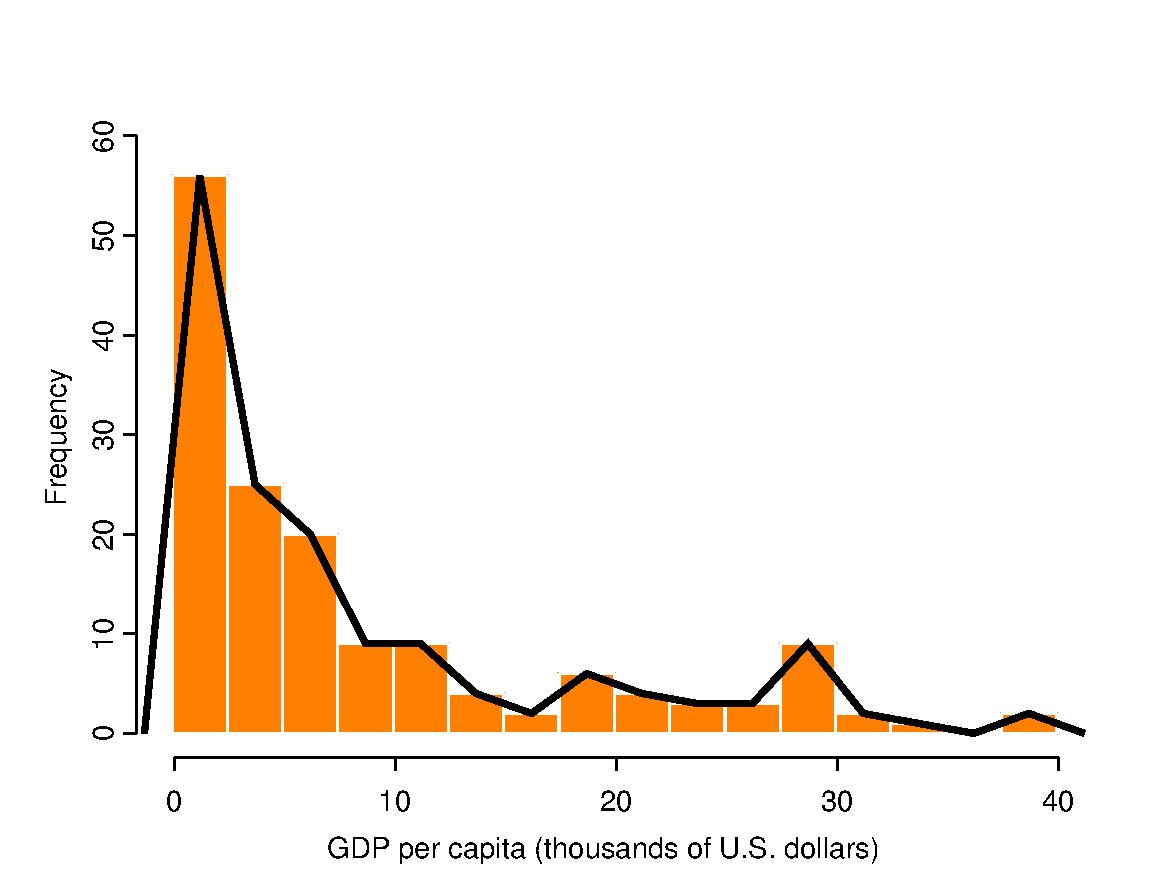
\includegraphics[width=13.50000cm]{gdp.pdf}
\caption{\label{fig:f-hist-gdp} Histogram of GDP per capita in the country
data, together with the corresponding frequency polygon.}
\end{figure}

A \textbf{histogram} is the graphical version of a frequency table for a
grouped variable, like that in Table \ref{tab:t-gdp}. Figure
\ref{fig:f-hist-gdp} shows a histogram for the GDP variable (the
histogram consists of the bars; the lines belong to a different graph,
the frequency polygon explained below). The basic idea of a histogram is
very similar to that of the bar chart, except that now the bars touch
each other to emphasise the fact that the original (ungrouped) variable
is considered continuous. Because the grouped variable is ordinal, the
bars of a histogram must be in the correct order.

A good choice of the grouping intervals of the variable and thus the
number of bars in the histogram is important for the usefulness of the
graph. If there are too few bars, too much information is obscured; if
too many, the shape of the histogram may become confusingly irregular.
Often the number of intervals used for a histogram will be larger than
what would be sensible for a table like \ref{tab:t-gdp}. Furthermore,
intervals like those in Table \ref{tab:t-gdp} are not even allowed in a
histogram, because they are of different widths (of 2, 3, 5, 10 and 10
units for the first five, and unbounded for the last one). The intervals
in a histogram must be of equal widths, because otherwise the visual
information in it becomes distorted (at least unless the histogram is
modified in ways not discussed here). For example, the intervals in
Figure \ref{fig:f-hist-gdp} (less than 2.5, 2.5--less than 5.0,
5.0--less than 7.5 etc.) are all 2.5 units wide. The exact choice can
usually be left to computer packages such as SPSS which use automatic
rules for choosing sensible intervals.

\subsubsection*{Frequency polygons}\label{frequency-polygons}
\addcontentsline{toc}{subsubsection}{Frequency polygons}

Figure \ref{fig:f-hist-gdp} also shows a \textbf{frequency polygon} of
the GDP variable. This is obtained by drawing lines to connect the
mid-points of the tops of the bars in a histogram. At each end of the
histogram the lines are further connected to zero, as if the histogram
had additional bars of zero height to the left and right of the smallest
and largest observed categories. The result is a curve with a similar
shape as the corresponding histogram, and its interpretation is similar
to that of the histogram.

A histogram is usually preferable to a frequency polygon for presenting
a single distribution, especially since histograms are typically much
easier to produce in standard software such as SPSS. However, frequency
polygons will later be useful for making comparisons between several
distributions.

\subsubsection*{Stem and leaf plots}\label{stem-and-leaf-plots}
\addcontentsline{toc}{subsubsection}{Stem and leaf plots}

A \textbf{stem and leaf plot} is a close relative of the histogram, and
is used for much the same purposes, mostly in small data sets. It is
easiest to explain through an example, so let us consider the GDP
variable again. The stem and leaf plot for it is shown in Figure
\ref{tab:t-stemgdp}. First, note that the values of the variable in the
sample (from \$500 to \$37800, recorded as 0.5 to 37.8 thousands of
dollars) have at most three significant digits. If the observations have
too many digits to be convenient for a stem and leaf plot, they can be
rounded first; for example, if the GDP figures had actually been
recorded down to the last dollar, we would have rounded them to the
nearest hundred dollars (as in Table \ref{tab:t-countrydata}) for the
plot. The last digit (here hundreds of dollars) will determine the
\emph{leaves} for the plot, while other digits (here round thousands of
dollars) will define the \emph{stem}.

\begin{longtable}[]{@{}ll@{}}
\caption{\label{tab:t-stemgdp} Stem and leaf plot of GDP per capita in the
country data (Stem=thousands of dollars, Leaf=hundreds of
dollars).}\tabularnewline
\toprule
\texttt{0} & \texttt{5566677778888899}\tabularnewline
\texttt{1} & \texttt{0001112233334445566677788899999}\tabularnewline
\texttt{2} & \texttt{1122234556799}\tabularnewline
\texttt{3} & \texttt{02334579}\tabularnewline
\texttt{4} & \texttt{00013567889}\tabularnewline
\texttt{5} & \texttt{014588}\tabularnewline
\texttt{6} & \texttt{0013334779}\tabularnewline
\texttt{7} & \texttt{002466}\tabularnewline
\texttt{8} & \texttt{9}\tabularnewline
\texttt{9} & \texttt{000159}\tabularnewline
\texttt{10} & \texttt{267}\tabularnewline
\texttt{11} & \texttt{12448}\tabularnewline
\texttt{12} & \texttt{38}\tabularnewline
\texttt{13} & \texttt{139}\tabularnewline
\texttt{14} &\tabularnewline
\texttt{15} & \texttt{7}\tabularnewline
\texttt{16} & \texttt{9}\tabularnewline
\texttt{17} & \texttt{8}\tabularnewline
\texttt{18} & \texttt{0}\tabularnewline
\texttt{19} & \texttt{0028}\tabularnewline
\texttt{20} & \texttt{0}\tabularnewline
\texttt{21} & \texttt{56}\tabularnewline
\texttt{22} & \texttt{0}\tabularnewline
\texttt{23} & \texttt{247}\tabularnewline
\texttt{24} &\tabularnewline
\texttt{25} &\tabularnewline
\texttt{26} & \texttt{78}\tabularnewline
\texttt{27} & \texttt{4667}\tabularnewline
\texttt{28} & \texttt{26}\tabularnewline
\texttt{29} & \texttt{0168}\tabularnewline
\texttt{30} & \texttt{0}\tabularnewline
\texttt{31} & \texttt{1}\tabularnewline
\texttt{32} & \texttt{7}\tabularnewline
\texttt{33} &\tabularnewline
\texttt{34} &\tabularnewline
\texttt{35} &\tabularnewline
\texttt{36} &\tabularnewline
\texttt{37} & \texttt{88}\tabularnewline
\bottomrule
\end{longtable}

The left-hand column in \ref{tab:t-stemgdp} lists the stem values in the
data, from smallest (0) to the largest (37). Each data value with the
same stem is represented on the same line by its leaf, i.e.~its last
digit. Thus the smallest value, 0.5 for Sierra Leone, is shown as a leaf
``5'' on the ``0'' stem, East Timor (another 0.5) as another ``5'' next
to it, and so on up to the largest value 37.8 for Norway, shown as an
``8'' leaf on the ``37'' stem.

The stem and leaf plot is very similar to a histogram (try turning
Figure \ref{tab:t-stemgdp} on its side, and compare to Figure
\ref{fig:f-hist-gdp}). It has the additional advantage that it also
shows the actual numerical values of the observations. In some rather
special cases this can reveal additional features of the data. Consider,
for example, the plot shown in Figure \ref{tab:t-stemhours}. The
variable here is the number of hours 86 respondents in a social survey
(a small subset of all the respondents, drawn purely for this
illustration) reported their \emph{spouse} worked in the previous week.
An obvious feature of the plot is the prevalence of zeroes as the
leaves, especially the many observations with 40 reported hours. This
suggests that most respondents probably did not carefully recall and add
up the exact hours their spouses worked the previous week; instead, a
round ``40'' is likely to be effectively a synonym for ``my spouse has a
regular nine-to-five job''. Such \emph{digit preference} is quite common
for many variables in surveys, and serves as a reminder that our
measurements are not always as precise as they may appear.

\begin{longtable}[]{@{}ll@{}}
\caption{\label{tab:t-stemhours} Stem and leaf plot of the reported hours
worked last week by the spouses of respondents in a social survey (the
data are a sample from data from the U.S. General Survey; observations
with less than 12 reported hours have been excluded). The stems and
leaves indicate tens of hours and single hours respectively. The main
disadvantage of a stem and leaf plot is that since every data value is
shown separately, the plot can only be used when the sample size is
relatively small. In such cases it is, however, a very useful and
user-friendly graph. Also, ``small'' does not mean ``tiny''. For
example, the country data set has as many as \(n=155\) observations, yet
Figure \ref{tab:t-stemgdp} is still quite readable and fits on a single
page.}\tabularnewline
\toprule
\texttt{1} & \texttt{55}\tabularnewline
\texttt{2} & \texttt{0000000555}\tabularnewline
\texttt{3} & \texttt{00002222556889}\tabularnewline
\texttt{4} &
\texttt{000000000000000000000000000000255556888}\tabularnewline
\texttt{5} & \texttt{000000355}\tabularnewline
\texttt{6} & \texttt{000000555}\tabularnewline
\texttt{7} & \texttt{022}\tabularnewline
\bottomrule
\end{longtable}

\begin{figure}[htbp]
\centering
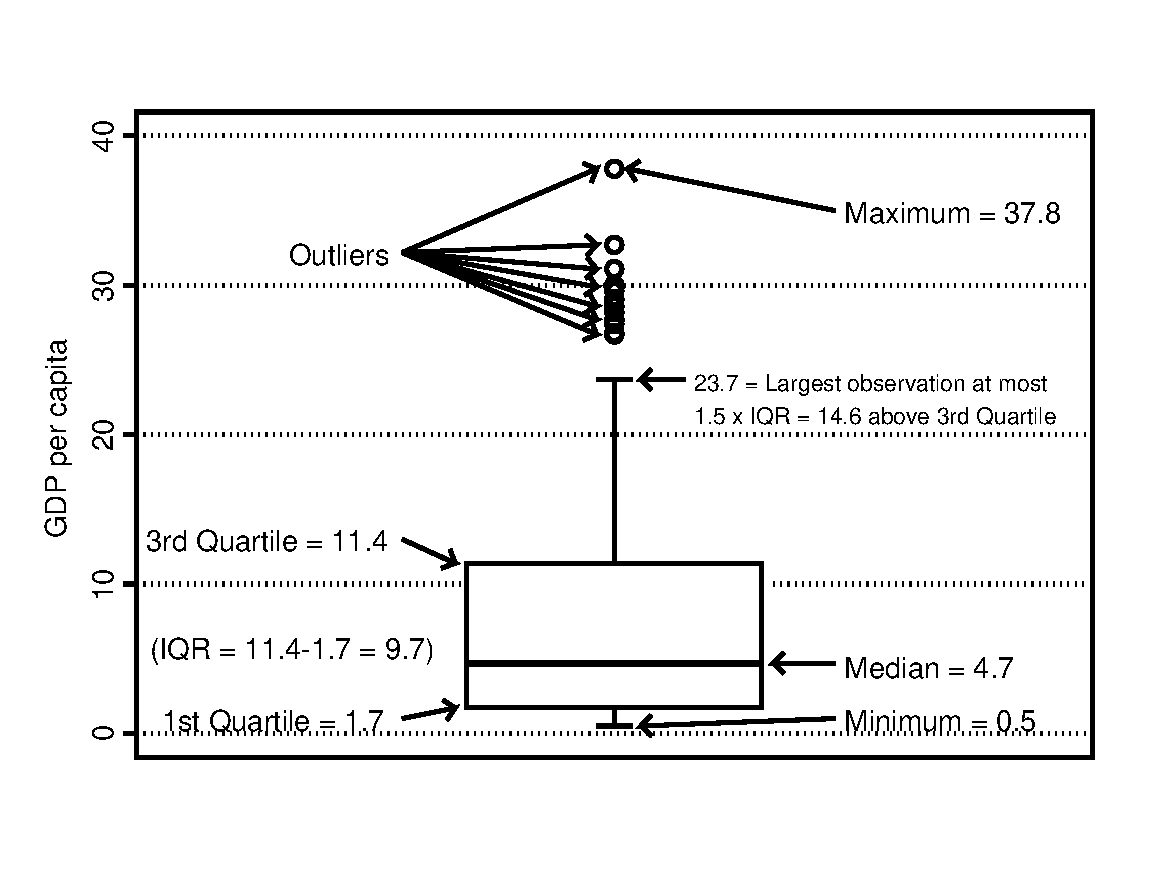
\includegraphics[width=15.00000cm]{box_gdp.pdf}
\caption{\label{fig:f-boxplot-gdp} An annotated box plot of GDP per capita
in the country data (\(n=155\)).}
\end{figure}

\subsubsection*{Box plots}\label{box-plots}
\addcontentsline{toc}{subsubsection}{Box plots}

A \textbf{box plot} differs from the graphs discussed so far in that it
does not attempt to display the whole distribution, but only certain
characteristics of it. The quantities included in a box plot are some of
the summary statistics defined in Section \ref{s-descr1-nums}. To
introduce the idea, one box plot is shown in Figure
\ref{fig:f-boxplot-gdp}. The variable considered here is again GDP per
capita. The vertical axis shows possible values of the variable, and the
plot itself contains the following elements:

\begin{itemize}
\item
  The line inside the central box is the \textbf{median} of the
  variable. Here it is 4.7.
\item
  The end points of the \textbf{box} are the \textbf{first and third
  quartile} of the variable, here 1.7 and 11.4 respectively. The length
  of the box is thus the interquartile range (IQR), here
  \(\text{IQR}=11.4-1.7=9.7\). The range of values covered by the box
  contains the middle 50\% of the observations. Half of the countries in
  this sample have GDPs between \$1700 and \$11400.
\item
  The two lines extending from the box on either side are known as the
  \textbf{whiskers}. Their length is determined as follows:

  \begin{itemize}
  \item
    Calculate the value of 1.5 times the IQR. This is the maximum length
    of each whisker. Here this is \(1.5\times 9.7=14.6\)
  \item
    The lower whisker extends to the smallest value (\textbf{minimum})
    of the variable in the sample, or to the smallest value which is at
    most 1.5\(\times\)IQR units below the first quartile, whichever is
    larger. Here the minimum is 0.5, which is less than 14.6 units below
    the first quartile of 1.7, so the lower whisker ends at 0.5.
  \item
    The upper whisker extends to the largest value (\textbf{maximum}) in
    the sample, or to the largest value which is at most
    1.5\(\times\)IQR units above the third quartile, whichever is
    smaller. Here the maximum is 37.8, which is further than the maximum
    distance of 14.6 above the third quartile of 11.4 allowed for a
    whisker. Thus the upper whisker could be drawn at most to
    \(11.4+14.6=26\). In this sample there are actually no observations
    of exactly 26, so the whisker ends at the next smallest observed
    value, which is 23.7.
  \end{itemize}
\item
  If the mimimum is further than 1.5\(\times\)IQR below the first
  quartile, or maximum further than 1.5\(\times\)IQR above the third
  quartile, there are still observations which are not in the range
  spanned by the box and the whiskers. Such extreme observations are
  considered \textbf{outliers} in the plot. The values for each outlier
  are plotted separately as points. Here there are 15 different outlying
  values, all with large values of the variable (because in two cases
  two countries have the same value, these 15 points actually represent
  17 countries).
\end{itemize}

A box plot thus shows some of the main features of a distribution with
the following visual cues:

\begin{itemize}
\item
  The central line shows a central value (the median) of the
  distribution.
\item
  The box shows the location of the central bulk (middle 50\%) of the
  observations
\item
  The whiskers show the range of the regular (non-outlying)
  observations.
\item
  Very extreme values (outliers), if any, are shown individually.
\end{itemize}

This can be quite effective for summarizing a distribution. For example,
a box plot where the median line is not roughly in the middle of the
box, or where one of the whiskers is much longer than the other,
indicates that the sample distribution is skewed in the direction of the
longer half of the box and the longer whisker. Here the distribution of
GDP per capita is clearly positively skewed, as we have already
observed. However, for a single distribution all such information and
more can also be obtained from a histogram. It is instead for
\emph{comparisons} of distributions between two or more samples that box
plots are particularly convenient, because it is easy to place two or
more of them side by side. This will be illustrated later in Section
\ref{ss-means-descr-graphs}.

\subsubsection*{Other graphs for single
variables}\label{other-graphs-for-single-variables}
\addcontentsline{toc}{subsubsection}{Other graphs for single variables}

Other types of graphs that are not described here are also sometimes
used for displaying distributions. One of them is a \textbf{pie chart},
which shows the proportions of the levels of a categorical (or grouped
continuous) variable as sectors of a circle. The relative area of a
sector indicates the proportion of the category. We will not discuss pie
charts further here, because we do not find them particularly useful
(the same information can usually be presented more clearly in a table,
bar chart or histogram). That, however, is partly a matter of taste, and
there is nothing inherently wrong with (clearly and properly presented)
pie charts.

\section{Numerical descriptive statistics}\label{s-descr1-nums}

The tabular and graphical methods discussed above aim to display the
whole sample distribution of a variable in an understandable form. The
methods introduced in this section have a different purpose. Each of
them is used to summarize some important single feature of the
distribution in one number. In general, any such number calculated from
the data is called a \textbf{statistic}. When it is used for data
description, it is a \textbf{descriptive statistic}, also known as a
\textbf{summary statistic}. This creates some terminological confusion,
as the phrase ``descriptive statistics'' can mean either all statistical
methods used for description or those statistics (i.e.~numbers
calculated from the data) with a descriptive purpose. The difference is
usually unimportant or clear from the context.

The two salient features of a distribution for which we will define
descriptive statistics are its \emph{central tendency} and its
\emph{variation}.

\subsection{Measures of central tendency}\label{ss-descr1-nums-central}

If you were allowed to know only one feature of the sample distribution
of a variable, chances are you would ask for something like its most
typical value, the middle value, or the average value --- in short, you
would be interested in a measure of \emph{central tendency}. We will
discuss three such measures below: the mode, the median and the mean
(corresponding, respectively, to the phrases ``most typical'',
``middle'' and ``average'' used above).

\subsubsection*{The mode}\label{the-mode}
\addcontentsline{toc}{subsubsection}{The mode}

The \textbf{mode} is the value of the variable which occurs most often
in the data, i.e.~the one with the highest frequency. For example,
Tables \ref{tab:t-region} and \ref{tab:t-democ} show that the mode of
the region variable in the country data is ``Africa'' and the mode of
the democracy score is 0. The GDP variable has two modes, 0.8 and 1.9,
which both appear five times (a distribution can have several modes; one
with two modes is said to be \emph{bimodal}).

The mode can be used for variables of any measurement level. For
\emph{nominal} variables it is the only available measure of central
tendency, as the median and the mean are not appropriate for such
variables.

The mode does not need to be a \emph{central} value in the sense that it
can even be the largest or smallest value of the variable, if this
occurs most often. This is the case for the democracy index in our
example.

The mode is most useful for categorical variables, where the number of
possible values is small, and the most common value thus has a high
frequency. With continuous variables (like GDP) and discrete variables
with many different values, the mode may be unstable and misleading. For
example, it is perfectly possible that all but one value appear once
each in a sample, and the mode is the value which happens to occur
twice.

\subsubsection*{The median}\label{the-median}
\addcontentsline{toc}{subsubsection}{The median}

Suppose that the values of a variable in a sample are first ordered from
the smallest to the largest. For example, in Table
\ref{tab:t-countrydata} the countries are ordered in this way according
to their GDP (starting from the bottom of the table). The
\textbf{median} is the value which falls in the middle of this ordering,
so that it divides the observed values into two halves. Because this
requires a meaningful ordering of the values, the median is appropriate
only for ordinal and interval-level variables, but not for nominal ones.

More specifically, suppose that there are \(n\) observations, indexed
from 1 for the smallest to \(n\) for the largest. The index of the
middle observation is then \((n+1)/2\). If \(n\) is an odd number, the
median is simply the observation in the ordered sample with this index.
If \(n\) is even, \((n+1)/2\) falls between two whole numbers, and the
median is the mean (of the kind defined below) of the observations with
these two indices. For example, in the country data set \(n=155\) (an
odd number), and \((n+1)/2=78\), so the median is the value of the 78th
observation in the ordered sample; if instead there had been \(n=156\)
countries, \((n+1)/2=78.5\), so the median would have been the mean of
the 78th and 79th observations.

In the country data set the median of the democracy score is 6, and the
median GDP is \$4700 (the 78th observation in GDP order is Paraguay). In
practice these are of course found using a a computer package like SPSS.
For an ordinal categorical variable like the democracy score the median
can also be found easily from the frequency table by considering the
\emph{cumulative percentages} (or proportions) of the categories. These
are obtained by adding up the percentages up to and including each
category, as shown in the last column of Table \ref{tab:t-democ}. The
median is then the category in which the cumulative percentage reaches
or passes 50\%. For the democracy index this happens for the score of 6,
which has a cumulative percentage of 50.9\%.

\subsubsection*{The mean}\label{the-mean}
\addcontentsline{toc}{subsubsection}{The mean}

The \textbf{mean} is the best-known and most widely used measure of
central tendency. It is also known as the \textbf{average}. To define
the mean, we need to introduce our first pieces of mathematical
notation. Suppose first that the variable of interest is denoted by
\(Y\). In practice the variable is of course called something else, like
GDP or Age or Income, but in the formulas below it is much more
convenient to refer to any such variable generically by one letter (note
also that the choice of the letter itself is arbitrary; for example, you
may often see \(X\) used instead of \(Y\) when the mean is defined).
Individual observations of \(Y\) are denoted generically by \(Y_{i}\),
where the subscript \(i\) identifies a single subject. The values of
\(i\) range from \(1\) to \(n\), so all of the observations in the
sample are \(Y_{1}, Y_{2}, \dots, Y_{n}\), e.g.~in the country example
(with \(n=155\)) \(Y_{1}, Y_{2}, \dots, Y_{155}\). The ordering of the
observations is arbitrary here, so it might for example be the order in
which they are listed in your SPSS data file. The mean \(\bar{Y}\)
(``Y-bar'') of the observations of \(Y\) in the sample is defined as

\begin{equation}\bar{Y} = \frac{\sum Y_{i}}{n}.
\label{eq:Ybar}\end{equation}

Here \(n\) is again the sample size. The symbol \(\Sigma\) (upper-case
Greek letter ``Sigma'') is a \emph{summation symbol}, which indicates
that we calculate the sum of all \(Y_{i}\) (often this is stated more
explicitly by the notation \(\sum_{i} Y_{i}\) or
\(\sum_{i=1}^{n} Y_{i}\) to make it clear that the summation is over all
the values of \(i\)). In other words, (\ref{eq:Ybar}) is a concise
expression for \[\bar{Y}= \frac{Y_{1}+Y_{2}+\dots+Y_{n}}{n}\] or, in
English, ``calculate the sum of all the observations of the variable
\(Y\) in the sample, and divide this sum by the number of observations
to obtain the mean of \(Y\) in the sample''. For example, for GDP per
capita this calculation gives
\[\bar{Y}= \frac{37.8+37.8+32.7+\dots+0.6+0.5+0.5}{155}
=\frac{1335.1}{155}=8.6\] (rounded to one decimal place), i.e.~mean GDP
among these countries is about \$8600.

Because the mean requires arithmetical calculations (summation and
division) on the observations \(Y_{i}\), it is strictly speaking only
appropriate for interval level variables, but not for ordinal ones, for
which the numbers of the categories are ordered labels rather than real
numbers. However, it is common to see this instruction ignored and means
calculated for ordinal variables, especially when they have a large
number of categories (see also the discussion under ``Measurement
Levels'' in Section \ref{ss-intro-def-vartypes}). For example, the mean
democracy score in our sample (using the codes 0--10 as its values) is
5.4. This may be used as a summary of the central tendency of the
variable, but it should not be overinterpreted as its meaning is not
quite as clear as that of, say, mean GDP.

For interval level variables the mean is by far the most commonly used
measure of central tendency. It does, however, have one arguably
undesirable feature. This is illustrated by the statistics for the GDP
variable, as shown in Table \ref{tab:t-countries-sums}. Its mean
(\$8600) is clearly much larger than the median (\$4700). This is due to
the shape of the distribution of GDP, as revealed by Figure
\ref{fig:f-hist-gdp} or even more clearly by the stem and leaf plot of
Figure \ref{tab:t-stemgdp}. While most of the countries are concentrated
around a fairly narrow range of GDPs, there are also a number of
countries with much larger GDPs. The ranges of values in the small and
large ends of the values in a distribution are (for fairly obvious
visual reasons) called the \textbf{tails} of the distribution. A
distribution with a (much) longer tail in one end than the other is said
to be \textbf{skewed}. A distribution like that of GDP in Figure
\ref{fig:f-hist-gdp}, with its long tail towards the large values, is
said to be \textbf{skewed to the right} or \textbf{positively skewed}. A
distribution shown in panel A of Figure \ref{fig:f-skews} is
\textbf{skewed to the left} (\textbf{negatively skewed}): while the
examination marks of most students are relatively high, there are some
students with very low marks. A distribution which has no clear skewness
in either direction, like the distribution of typical weekly working
hours in panel B of Figure \ref{fig:f-skews} is (approximately)
\textbf{symmetric}.

\begin{longtable}[]{@{}lrccccc@{}}
\caption{\label{tab:t-countries-sums} Summary statistics for the three
variables in the country data. IQR=interquartile range; s.d.=standard
deviation; *: inappropriate for a nominal variable; \(\dagger\): if the
democracy index is treated as an interval-level
variable.}\tabularnewline
\toprule
\begin{minipage}[b]{0.12\columnwidth}\raggedright\strut
\\strut
\end{minipage} & \begin{minipage}[b]{0.11\columnwidth}\raggedleft\strut
Measures\strut
\end{minipage} & \begin{minipage}[b]{0.23\columnwidth}\centering\strut
of central\strut
\end{minipage} & \begin{minipage}[b]{0.09\columnwidth}\centering\strut
tendency\strut
\end{minipage} & \begin{minipage}[b]{0.09\columnwidth}\centering\strut
Measures\strut
\end{minipage} & \begin{minipage}[b]{0.08\columnwidth}\centering\strut
of\strut
\end{minipage} & \begin{minipage}[b]{0.09\columnwidth}\centering\strut
variation\strut
\end{minipage}\tabularnewline
\midrule
\endfirsthead
\toprule
\begin{minipage}[b]{0.12\columnwidth}\raggedright\strut
\\strut
\end{minipage} & \begin{minipage}[b]{0.11\columnwidth}\raggedleft\strut
Measures\strut
\end{minipage} & \begin{minipage}[b]{0.23\columnwidth}\centering\strut
of central\strut
\end{minipage} & \begin{minipage}[b]{0.09\columnwidth}\centering\strut
tendency\strut
\end{minipage} & \begin{minipage}[b]{0.09\columnwidth}\centering\strut
Measures\strut
\end{minipage} & \begin{minipage}[b]{0.08\columnwidth}\centering\strut
of\strut
\end{minipage} & \begin{minipage}[b]{0.09\columnwidth}\centering\strut
variation\strut
\end{minipage}\tabularnewline
\midrule
\endhead
\begin{minipage}[t]{0.12\columnwidth}\raggedright\strut
Variable\strut
\end{minipage} & \begin{minipage}[t]{0.11\columnwidth}\raggedleft\strut
Mode\strut
\end{minipage} & \begin{minipage}[t]{0.23\columnwidth}\centering\strut
Median\strut
\end{minipage} & \begin{minipage}[t]{0.09\columnwidth}\centering\strut
Mean\strut
\end{minipage} & \begin{minipage}[t]{0.09\columnwidth}\centering\strut
Range\strut
\end{minipage} & \begin{minipage}[t]{0.08\columnwidth}\centering\strut
IQR\strut
\end{minipage} & \begin{minipage}[t]{0.09\columnwidth}\centering\strut
s.d.\strut
\end{minipage}\tabularnewline
\begin{minipage}[t]{0.12\columnwidth}\raggedright\strut
Region\strut
\end{minipage} & \begin{minipage}[t]{0.11\columnwidth}\raggedleft\strut
Africa\strut
\end{minipage} & \begin{minipage}[t]{0.23\columnwidth}\centering\strut
*\strut
\end{minipage} & \begin{minipage}[t]{0.09\columnwidth}\centering\strut
*\strut
\end{minipage} & \begin{minipage}[t]{0.09\columnwidth}\centering\strut
*\strut
\end{minipage} & \begin{minipage}[t]{0.08\columnwidth}\centering\strut
*\strut
\end{minipage} & \begin{minipage}[t]{0.09\columnwidth}\centering\strut
*\strut
\end{minipage}\tabularnewline
\begin{minipage}[t]{0.12\columnwidth}\raggedright\strut
Democracy index\strut
\end{minipage} & \begin{minipage}[t]{0.11\columnwidth}\raggedleft\strut
0\strut
\end{minipage} & \begin{minipage}[t]{0.23\columnwidth}\centering\strut
6\strut
\end{minipage} & \begin{minipage}[t]{0.09\columnwidth}\centering\strut
5.4\(^{\dagger}\)\strut
\end{minipage} & \begin{minipage}[t]{0.09\columnwidth}\centering\strut
10\(^{\dagger}\)\strut
\end{minipage} & \begin{minipage}[t]{0.08\columnwidth}\centering\strut
8\(^{\dagger}\)\strut
\end{minipage} & \begin{minipage}[t]{0.09\columnwidth}\centering\strut
3.9\(^{\dagger}\)\strut
\end{minipage}\tabularnewline
\begin{minipage}[t]{0.12\columnwidth}\raggedright\strut
GDP per capita\strut
\end{minipage} & \begin{minipage}[t]{0.11\columnwidth}\raggedleft\strut
\$800 and \$1900\strut
\end{minipage} & \begin{minipage}[t]{0.23\columnwidth}\centering\strut
\$4700\strut
\end{minipage} & \begin{minipage}[t]{0.09\columnwidth}\centering\strut
\$8600\strut
\end{minipage} & \begin{minipage}[t]{0.09\columnwidth}\centering\strut
\$37300\strut
\end{minipage} & \begin{minipage}[t]{0.08\columnwidth}\centering\strut
\$9700\strut
\end{minipage} & \begin{minipage}[t]{0.09\columnwidth}\centering\strut
\$9450\strut
\end{minipage}\tabularnewline
\bottomrule
\end{longtable}

\begin{figure}[htbp]
\centering
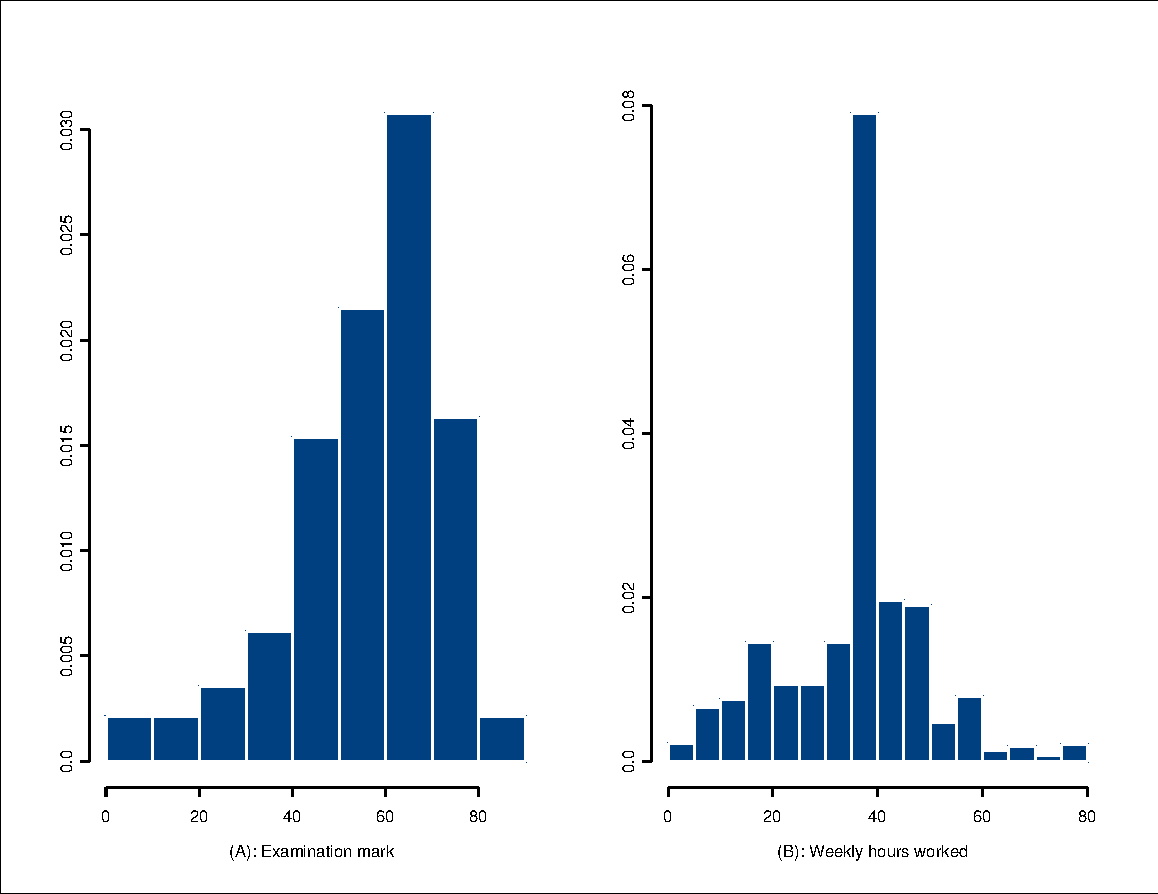
\includegraphics[width=14.00000cm]{twohists.pdf}
\caption{\label{fig:f-skews} Examples of a negatively skewed and an
approximately symmetric sample distribution. Panel A shows the
distribution of examination marks for MY451 (2003; \(n=419\)), and B
shows the distribution of the number of hours a person usually works in
their main job in the 3 per cent Individual Sample of Anonymized Records
from the 2001 U.K.~Census (\(n=867,016\), respondents with hours 0 or
not applicable omitted) Source of the data for panel B: Cathie Marsh
Centre for Census and Survey Research, University of Manchester,
\url{http://www.ccsr.ac.uk/sars/}.}
\end{figure}

The mean is almost always further in the direction of skewness than the
median. That is why the mean of the positively skewed GDP variable is
larger than its median. In general, a comparison between the two
statistics will reveal the direction of any skewness, and give an
indication of its magnitude. When the difference is large, as it is
here, it is typically sensible to report both the mean and the median.

The mean is sensitive even to individual observations far in the tails
of the distribution. Such observations, which are very different (much
larger or smaller) from the rest of the data, are known as
\textbf{outliers}. Even a single outlier can, if it is extreme enough,
pull the mean far towards itself, even beyond the range of all the other
observations, as in the following example:

\emph{Example: A sample with an outlier}\\
Suppose that an M.Sc.~student, preparing her dissertation on elements of
social capital in Canada, is examining various measures of community
activities in a sample of fourty municipalities in the province of
Manitoba\footnote{Strictly speaking, the analysis should incorporate
  sampling weights (variable \emph{DWEIGHT}) to adjust for different
  sampling probabilities for different types of respondents. Here the
  weights are ignored. Using them would not change the main conclusions
  for these variables.}. As part of an initial description of these
communities, she wants to summarize their populations, which are

5, 79, 143, 226, 303, 317, 384, 417, 448, 505, 524, 525, 538, 619, 621,
629, 637, 760, 801, 906, 955, 959, 964, 1047, 1111, 1152, 1457, 1491,
1722, 1907, 2079, 2405, 2723, 3950, 4012, 4032, 4183, 4427, 12602,
619544.

The outlier in this case is the city of Winnipeg, whose population of
nearly 620,000 is 49 times as large as that of the next largest
municipality in the sample. With it included in the sample, the mean
population of the 40 municipalities is about 17000; without it, the mean
for the other 39 is 1600. The two numbers give rather different pictures
of the size of an ``average'' community in the data (similar differences
would probably be observed for other variables too, so the large city
would be an outlier in many respects in a study like this). The median,
on the other hand, is 906 for the 39 smaller communities, and 930.5 with
Winnipeg included. It is thus essentially unaffected by the outlier,
basically because it is only influenced by the fact that 619,554 is
bigger than the mid-point of the data, but not by how much bigger it is.

\subsection{Measures of variation}\label{ss-descr1-nums-variation}

A measure of central tendency is not a complete summary of a
distribution, in that there can be distributions which have the same
central tendency but which are different in some other respect. To
illustrate this with a hypothetical example, suppose we are studying the
students in three classrooms of the same grade at a local school. Each
class has 14 students, and all students have just taken the same test,
graded 1 (low) to 10 (high). The marks of the students are found to be
as shown in Table \ref{tab:t-classmarks}.

Both the mean and the median of the marks are 6 in every class. However,
the classes are otherwise clearly not similar. In particular, the
\textbf{variation} (or \textbf{dispersion}) of the marks is very
different. There is no variation at all in Class 1 where everyone has
the same score, and quite a lot of variation in Class 3, while Class 2
seems to fall between the two. To capture this, some \textbf{measure of
variation} will be needed. Three such measures are described here. All
of them stricly speaking require the variable to be measured at an
interval level, because they involve calculations of differences between
its values. Using them on an ordinal variable is thus subject to similar
cautions as for the mean above. These measures of variation are entirely
inappropriate for nominal-level variables. There are some measures which
can be used for such variables, but they are not described here.

\begin{longtable}[]{@{}ll@{}}
\caption{\label{tab:t-classmarks} A hypothetical examples of test marks of
students in three classes.}\tabularnewline
\toprule
Class 1: & 6 6 6 6 6 6 6 6 6 6 6 6 6 6\tabularnewline
Class 2: & 4 4 5 5 5 6 6 6 6 7 7 7 8 8\tabularnewline
Class 3: & 1 2 2 3 4 4 4 8 8 9 9 10 10 10\tabularnewline
\bottomrule
\end{longtable}

\subsubsection*{Range}\label{range}
\addcontentsline{toc}{subsubsection}{Range}

The \textbf{range} of a variable is simply the difference between its
largest and smallest observed values (the \textbf{maximum} and
\textbf{minimum} in statistical terminology). In the class example
above,

Class 1: Range \(= 6-6 =0\)\\
Class 2: Range \(= 8-4 =4\)\\
Class 3: Range \(= 10-1 =9\)

The measure is largest for Class 3 and smallest for Class 1, so it seems
to capture the differences in variation suggested by an initial look at
the numbers themselves. For Class 1 the range is 0, because all of the
observations are the same. In general, any sensible measure of variation
should be zero when there is no variation (all observations are
identical), and all of the measures described here have that property.

In the country data, the range of GDP is \$37800-\$500=\$37300, and the
range of the democracy score (if we cautiously treat it as an
interval-level variable) is 10-0=10.

\subsubsection*{Interquartile range}\label{interquartile-range}
\addcontentsline{toc}{subsubsection}{Interquartile range}

The range is often not a particularly useful measure of variation,
because it depends \emph{only} on the two extremes of the data. It is
thus very sensitive to outliers. If, for example, there is one large
outlier, the range will be large even if all of the other observations
are very similar to each other.

One way to reduce the effects of outliers is to ignore the tails of the
distribution and consider the variation only among the central range of
the data. This idea is expressed in the \textbf{Interquartile range}.
First we have to define the quartiles:

\begin{itemize}
\item
  \textbf{The first quartile} is the value such that 25\% (one quarter)
  of the observations are smaller than (or equal to) it, and 75\% (three
  quarters) bigger than (or equal to) it.
\item
  \textbf{The third quartile} is the value such that 75\% of the
  observations are smaller than (or equal to) it, and 25\% bigger than
  (or equal to) it.
\end{itemize}

The quartiles are thus similar in spirit to the median. Just as the
median divides the observations into two equal halves (those below and
those above the median), the quartiles divide them into two groups at
different points. For example, the first quartile divides the
observations into the smallest 25\% and the remaining largest 75\%. (The
median can thus also be described as the \emph{second quartile}, and all
of these statistics are special cases of a larger class of similar
statistics known as \emph{percentiles}.)

The interquartile range (IQR) is the difference between the third and
the first quartile. It is the range of the middle 50\% of the
observations, leaving out the smallest 25\% and the largest 25\%. This
effectively eliminates the effects of any outliers, so IQR is a useful
measure of variation (often used together with the median as measure of
central tendency) when there are serious outliers or when the
distribution is very skewed.

For the class example the interquartile ranges are

Class 1: IQR \(= 6-6 =0\)\\
Class 2: IQR \(= 7-5 =2\)\\
Class 3: IQR \(= 9.25-2.75 =6.5\)

These are again in the expected order.\footnote{The data can be obtained
  from \texttt{http://bes2009-10.org/}, which gives further information
  on the survey, including the full text of the questionnaires. The data
  analysed in this class and homework are from the BES Campaign Internet
  Panel Survey, which has been divided into two data sets corresponding
  to two time periods leading up to the General Election.} For the
country data, the first and third quartiles for GDP are 1.7 and 11.4
respectively, and IQR=11.4-1.7=9.7. For the democracy score the
quartiles are 1 and 9, and IQR=8.

\subsubsection*{Standard deviation}\label{standard-deviation}
\addcontentsline{toc}{subsubsection}{Standard deviation}

The most commonly used measure of variation is based on the
\textbf{deviations} \[Y_{i}-\bar{Y}\] where \(Y_{i}\) again denotes an
individual observation of a variable, and \(\bar{Y}\) is its mean. A
deviation is the difference between an individual observation and the
average value in the sample. Table \ref{tab:t-sdex} shows the deviations
for Class 3 in the class example, together with the other calculations
discussed below. Here a negative deviation indicates that an observation
is smaller than the mean of 6 (e.g. \(1-6=-5\)), and a positive
deviation that an observation is larger than the mean
(e.g.~\(10-6=+4\)).

\begin{longtable}[]{@{}lrrr@{}}
\caption{\label{tab:t-sdex} Calculating the standard deviation of test marks
for Class 3 in the class example at the beginning of Section
\ref{ss-descr1-nums-variation}.}\tabularnewline
\toprule
Student & \(Y_{i}\) & \(Y_{i}-\bar{Y}\) &
\((Y_{i}-\bar{Y})^{2}\)\tabularnewline
1 & 1 & \(-5\) & 25\tabularnewline
2 & 2 & \(-4\) & 16\tabularnewline
3 & 2 & \(-4\) & 16\tabularnewline
4 & 3 & \(-3\) & 9\tabularnewline
5 & 4 & \(-2\) & 4\tabularnewline
6 & 4 & \(-2\) & 4\tabularnewline
7 & 4 & \(-2\) & 4\tabularnewline
8 & 8 & +2 & 4\tabularnewline
9 & 8 & +2 & 4\tabularnewline
10 & 9 & +3 & 9\tabularnewline
11 & 9 & +3 & 9\tabularnewline
12 & 10 & +4 & 16\tabularnewline
13 & 10 & +4 & 16\tabularnewline
\(14=n\) & 10 & +4 & 16\tabularnewline
Sum & \(\sum Y_{i}=84\) & \(\sum(Y_{i}-\bar{Y})=0\) &
\(\sum(Y_{i}-\bar{Y})^{2}=152\)\tabularnewline
& \(\bar{Y}=84/14=6\) & \(\sum(Y_{i}-\bar{Y})/n=0\) &
\(s^{2}=152/13=11.69\)\tabularnewline
& & & \(s=\sqrt{11.69}=3.4\)\tabularnewline
\bottomrule
\end{longtable}

The deviations are clearly related to variation, as a sample with little
variation will have small deviations (most observations are close to the
mean) and one with a lot of variation will have many large deviations
(many observations are far from the mean). All that remains is to
aggregate them in some sensible way into a single number.

An inappropriate summary of the deviations is their mean,
i.e.~\(\sum (Y_{i}-\bar{Y})/n\). In the class example this turns out to
be zero (see the second column of Table \ref{tab:t-sdex}), and not by
coincidence. It can be shown that the mean of the deviations is in fact
zero for any set of numbers. This happens because positive and negative
deviations will always exactly cancel out each other in the sum. This is
clearly not what we want, because a negative deviation of, say, \(-2\)
(an observation two units below the mean) should be equally strong
evidence of variation as a positive deviation of +2 (an observation two
units above the mean). The signs of the deviations thus need to be
eliminated somehow. Just dropping the negative signs (so that \(-2\)
becomes 2) means calculating the \emph{absolute values} of the
deviations, denoted \(|Y_{i}-\bar{Y}|\). Taking the mean of these gives
the \textbf{mean absolute deviation} or MAD, defined as
\[\text{MAD}=\frac{\sum |Y_{i}-\bar{Y}|}{n}.\] This is a perfectly
sensible measure of variation, but it is not very commonly used. This is
largely because absolute values are mathematically rather difficult to
work with, and this would make MAD very inconvenient for more
sophisticated analyses, where measures of variation will also be
needed.\footnote{Official results obtained from
  \texttt{www.olympic.org/london-2012-summer-olympics}.} Instead, we
eliminate the signs of the deviations by using their squares
\((Y_{i}-\bar{Y})^{2}\), i.e.~by multiplying each deviation by itself
(c.f. the third column of Table \ref{tab:t-sdex} for an illustration).
These are used to calculate the \textbf{variance}, denoted \(s^{2}\) and
defined as

\begin{equation}s^{2} = \frac{\sum (Y_{i}-\bar{Y})^{2}}{n-1}.
\label{eq:samplevar}\end{equation}

This is (apart from the \(n-1\) rather than \(n\) as the divisor)
essentially the mean of the squared deviations. Its units of measurement
are also squares of the units of the original measurements. For example,
the variance of the GDP variable, which is itself measured in (thousands
of) dollars, is expressed in dollars squared. This is rather
inconvenient for any meaningful interpretation. To obtain a measure of
variation expressed in the original units, we can take the square root
(indicated below by \(\sqrt{\; \; }\)) of the variance. This statistic
is the \textbf{standard deviation}, often abbreviated as S.D., denoted
by \(s\) and defined as

\begin{equation}s = \sqrt{\frac{\sum (Y_{i}-\bar{Y})^{2}}{n-1}.}
\label{eq:sd}\end{equation}

For the class example, this is 0 for Class 1, 1.3 for Class 2, and 3.4
for class 3. In the country data, the standard deviation of GDP is
\$9450 and that of the democracy score (if it is treated as an
interval-level variable) is 3.9, as shown in Table
\ref{tab:t-countries-sums}.

Like the mean, the standard deviation is sensitive to outliers and
skewness of the distribution, so sometimes other measures of variation
(e.g.~IQR or MAD) should be reported instead of, or in addition to it.
Nevertheless, the standard deviation is by far the most commonly used
measure of variation. One reason for this is that it is very important
not just as a descriptive statistic but also as an element in several
forms of statistical inference. For description it is typically less
immediately interpretable than measures of central tendency. Often the
most revealing descriptive uses of the standard deviation are in
comparisons between samples, like in the class example above. The
following is a real example of this kind, where variation was in fact of
more interest than central tendency:

\emph{Example: Variation in rates of economic growth}\\
In an article titled ``Dancing in step'' on November 13th 2004,
\emph{The Economist} discussed a set of data (collected by the J.~P.
Morgan Chase bank) on the annual growth rates (in percentage points) of
the Gross Domestic Products (GDP) of 30 countries for each year since
1971. Measures of central tendency, such as average growth rates for
each country and each year, are clearly interesting in this case.
However, most of the discussion in the article concerned
\emph{variation} in growth rates, measured by their standard deviation
across countries for each year, and especially changes in this variation
over time. The standard deviation of growth rates was around 3--5
percentage points for every year until the early 1990s, had fallen to
about 2 percentage points in 2003, and was forecast to decline further
in subsequent years. There had thus previously been a fair amount of
variation in rates of economic growth (with some economies growing
faster and some slower, some perhaps being in recession), whereas
recently the growth rates had become more similar across countries. The
article summarized this in its subtitle as ``The world's economies are
more synchronised than ever before'', and went on to discuss the
implications of this development for global economy.

The formula (\ref{eq:sd}) for the standard deviation involves the
divisor \(n-1\), where the discussion leading up to it might make you
expect \(n\) instead. The reasons for this will be discussed briefly in
Section \ref{ss-contd-popdistrs-params}. The definition is not entirely
consistent in that some textbooks do use \(n\) instead of \(n-1\). The
difference is of no great importance, and using either \(n\) or \(n-1\)
would be fine for our purposes. Whenever \(n\) is even moderately large,
the difference between \(n\) and \(n-1\) is in any case small, and both
definitions of standard deviation give very similar values.

Finally, measures of central tendency and measures of variation, even
though they summarise the two most important features of a sample
distribution of a variable, may still miss some important features of
the distribution. Consider, for example, the class marks in Classes 2
and 3 in our hypothetical example. These are summarized by the bar
charts of Figure \ref{fig:f-classbars}. The distribution for Class 2 is
symmetric and concentrated around the mean value of 6. The most
noticeable feature of the marks in Class 3, on the other hand, is that
there appear to be two distinct groups of students, one with very low
scores and one with high scores. A similar feature was also noted in the
distribution of the democracy index in the country data (c.f.~Figure
\ref{fig:f-bars-democ}). This property would not be revealed by measures
of central tendency or variation, so it is an illustration of why it is
always sensible to also examine the whole distribution of a variable
using frequency tables or graphical methods.

\begin{figure}[htbp]
\centering
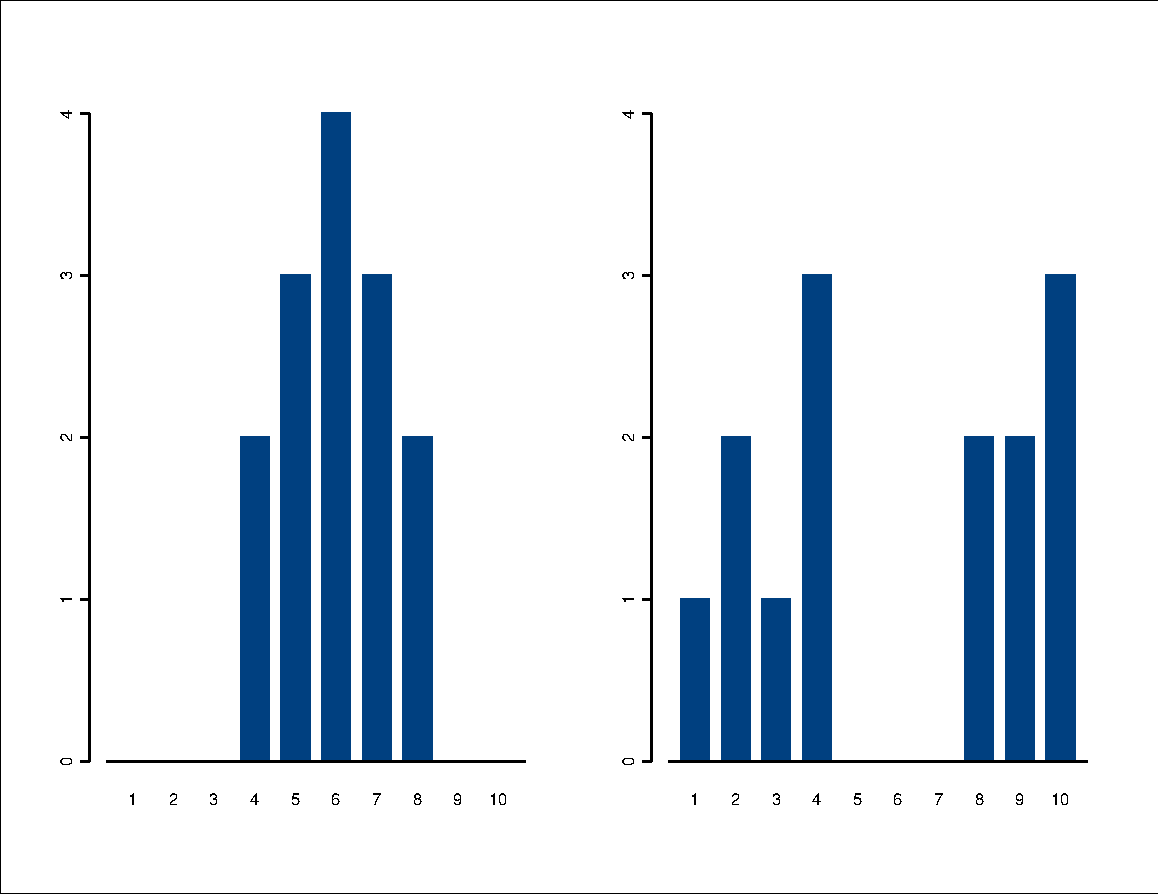
\includegraphics[height=8.30000cm]{classbars.pdf}
\caption{\label{fig:f-classbars} Bar charts of the test marks in the class
example at the beginning of Section \ref{ss-descr1-nums-variation} for
Classes 2 (on the left) and 3 (on the right).}
\end{figure}

\section{Associations which involve continuous
variables}\label{s-descr1-2cont}

Bivariate descriptive methods which are designed for situations where at
least one of the two variables is continuous are not described here but
in later sections:

\begin{itemize}
\item
  Explanatory variable is categorical and response variable continuous:
  Parallel histograms, frequency polygons and box plots (Section
  \ref{s-means-descr}).
\item
  Both explanatory and response variables are continuous: Scatter plots
  and line plots (Section \ref{ss-regression-descr-plots}).
\end{itemize}

We do not discuss the remaining possibility, where the explanatory
variable is continuous and the response is categorical. The simplest and
usually quite sufficient way to give an initial description of the
associations in this case is to group the explanatory variable into a
categorical variable and then apply the methods of Section
\ref{s-descr1-2cat}.

\section{Presentation of tables and graphs}\label{s-descr1-presentation}

The purpose of statistical tables and graphs is to communicate
information correctly, clearly and effectively. If they do not do that,
that is, if they leave the reader misled, confused or uninformed, they
have failed and should not have been shown at all. Creating good tables
and graphics is not only a matter of understanding the technical details
described above. It also involves general principles of design and
presentation. Most of these should be simple common sense but clearly
are not, judging by the many entirely unhelpful tables and graphs
appearing in all kinds of publications. This section discusses very
briefly some principles of good practice in presenting descriptive
statistics in tables and graphs. Much of the section is based on two
books, \emph{The Visual Display of Quantitative Information} by Edward
R.~Tufte (Graphics Press, 1983) and \emph{Visual Revelations} by Howard
Wainer (Copernicus, 1997). These can be consulted for further
information and examples of both good and bad practice.

First, a reader of a table or graph should be able to understand what it
is about:

\begin{itemize}
\item
  The variables should be labelled clearly. In particular, the names
  used in computer data files should not be used unless they are also
  understandable words. So even if a variable is called ATTDFOXH in your
  SPSS file, it should still be labelled ``Attitude to foxhunting''or
  something similar in presentation. Similarly, the categories of
  variables should be labelled in words wherever appropriate.
\item
  Items such as the columns of a table or the vertical axis of a bar
  chart should also be labelled clearly (e.g.~whether they are for
  frequencies or percentages).
\item
  More generally, a table or figure and its caption should be (within
  reason) as self-contained as possible, in that the reader should be
  able to understand them with little reference to the rest of the text
  for explanation (remember that tables and figures often float,
  i.e.~they may appear on a different page from where they are referred
  to in the main text). This may also include giving the source of the
  data in a note or caption to the table or figure.
\end{itemize}

Some guidelines for constructing tables are

\begin{itemize}
\item
  A table produced by software such as SPSS, although it contains the
  necessary numbers, is rarely suitable for presentation directly.
  Tables included in research reports should be retyped and reformatted.
\item
  The categories of the variable should be in a sensible order. For
  ordinal variables (including those obtained by grouping a continuous
  one), this should obviously be the natural ordering of the categories.
  For a nominal variable, the order can be chosen in whichever way is
  most useful for presentation. Often it makes sense to order categories
  from the largest to the smallest, typically leaving any ``Others''
  category last.
\item
  If only proportions or percentages are shown, the sample size \(n\)
  should also be reported, perhaps in a note or caption to the table.
  This will allow the reader to judge how informative the table is. A
  percentage of 20\% is clearly richer information when it corresponds
  to a frequency of 2,000 in a sample 10,000 than when it means 2 out of
  10 observations. When \(n\) is very small, proportions and percentages
  should be avoided altogether: reporting 1 out 7 as 14.3\% is simply
  nonsensical.
\item
  Proportions and percentages can and should be rounded. It is rarely
  necessary to see percentages with more than one decimal place, if even
  that.
\end{itemize}

With graphs, it is always useful to bear in mind Wainer's principle:

\textbf{The aim of good data graphics is to}\\
\textbf{display data accurately and clearly}

The way to produce \emph{bad} graphs is thus to break some part of this,
for example by (1) not showing much data, (2) showing much that is not
data, (3) showing the data inaccurately, or (4) obscuring the data.
Graphs with these characteristics are a form of visual lying, distorting
the graphical cues in a plot in ways which make it difficult or
impossible to obtain accurate information from it.

One example of a lying graph already mentioned is the ``cut'' bar chart
where the bars do not begin at zero. Another is the pseudo third
dimension, an example of which is shown in Figure \ref{fig:f-yuk}. The
information presented in this graph is the same as that of Figure
\ref{fig:f-bars-region}, i.e.~frequencies of different regions. These
are represented by the heights of the bars. The additional information
conveyed by the apparent thickness of the bars, represented in
perspective to give an illusion of three-dimensional bars, is then ---
exactly nothing. The fake third dimension represents no data, and serves
only to distort the real data that are being shown.

We can thus give a simple instruction: using a fake third dimension like
the one in Figure \ref{fig:f-yuk} is always wrong and not acceptable
under any circumstances. This is true irrespective of the fact that such
graphs are often seen and easily (often almost automatically) produced
by software packages like Microsoft Excel. All this proves is that the
programmers of those packages have little graphical sense, or perhaps
that their companies have discovered that their customers are willing to
pay for such ``features'' as colourful but pointless graphs. Indeed,
many if not most of the graph styles provided by, say, Excel (exploding
pie charts, doughnuts, cones, pyramids and so on) are entirely useless
for accurate presentation of data.

\begin{figure}[htbp]
\centering
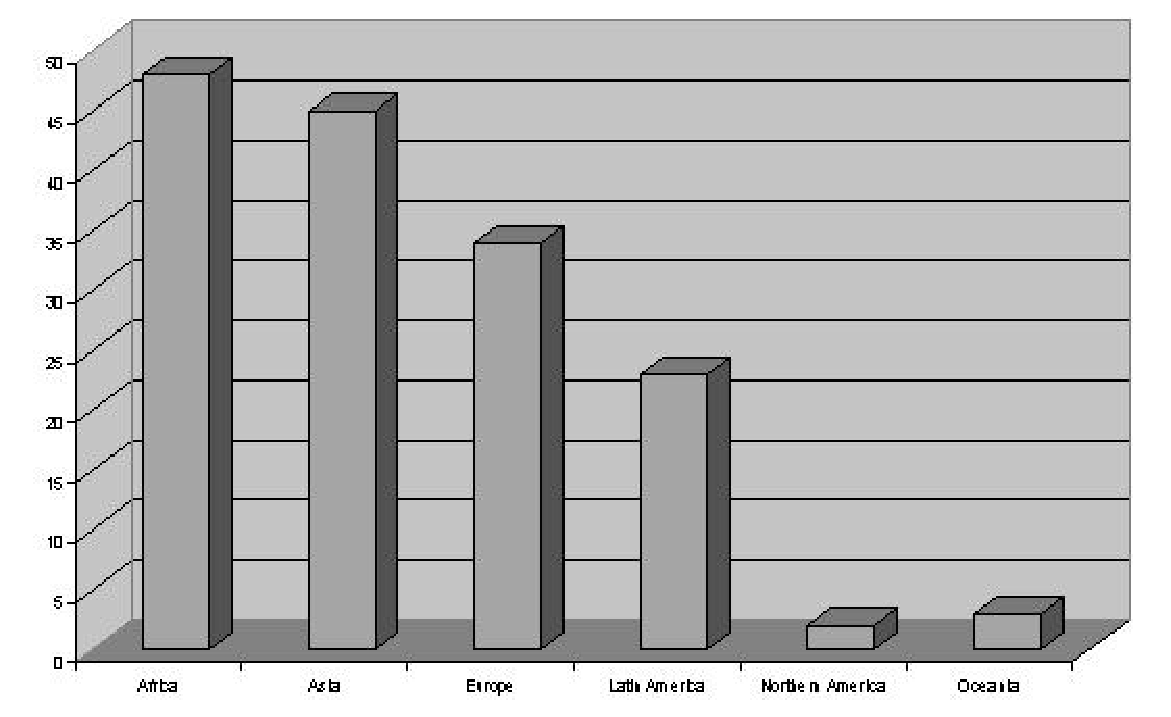
\includegraphics[height=8.00000cm]{threeD.pdf}
\caption{\label{fig:f-yuk} An example of an unacceptable graph: a bar chart
with a pseudo three-dimensional effect. The data are the same as in
Figure \ref{fig:f-bars-region}.}
\end{figure}

An objection sometimes offered to such a severe rule is that bad graphs
``look good''. This can be answered in two ways. First, a statistical
graphic is not a decoration, but a tool for presenting information.
Authors who confuse the two often end up displaying pretty colours and
strange shapes to hide the lack of actual information in a graph.
Second, even in an aesthetic sense a useful and accurate graph is
preferable to a bad one, in the way that any well-designed object with a
function tends to be more attractive than a badly designed one.

What, then, is the recipe for good graphics? Mostly this is just a
matter of using basic graph types in a sensible and restrained manner,
focusing on presenting information and avoiding all distracting
decoration. Some such examples have been given earlier in this chapter.
Other types of graphs are used to illustrate associations between
variables, which we have not yet discussed. To anticipate that a little,
Figure \ref{fig:f-houseprices} shows one (good but not in any way
exceptional) example of such graphs. It is a reproduction of a graph
originally published in a survey of Spain in \emph{The Economist}, and
shows changes in average house prices in Spain, Germany and Britain
between 1993 and 2003. Even without an introductory statistics course,
the main message of Figure \ref{fig:f-houseprices} is immediately clear:
increases in Spanish house prices over the period have been comparable
to those in Britain, with prices more than doubling in both countries,
and very unlike those in Germany, where the prices have remained
unchanged. Note also that the graph distinguishes between the lines for
different countries by using different types of line. Different colours
can of course be used instead, but their differences will become
obscured if the graph is photocopied or printed in black and white.

\begin{figure}[htbp]
\centering
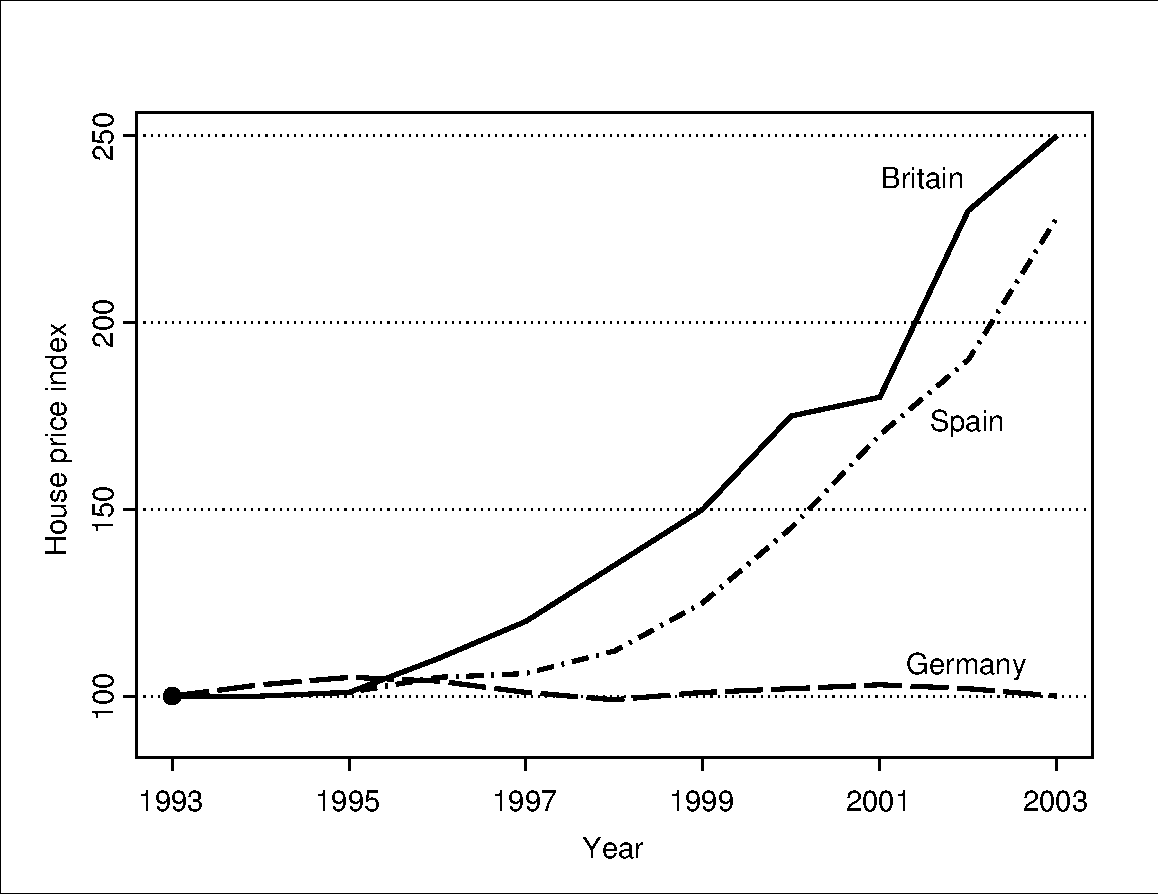
\includegraphics[width=10.00000cm]{houseprices.pdf}
\caption{\label{fig:f-houseprices} An example of an informative graph: house
prices in three countries between 1993 and 2003, indexed to 100 in 1993.
Source: \emph{The Economist}, June 26th, 2004. The numbers were
estimated from the graph in the magazine, so they are approximate.}
\end{figure}

In addition to such modest but sensible and useful basic graphs, you may
sometimes encounter inspired examples of special graphs which manage to
describe particular data sets in exceptionally vivid and informative
ways. Some such examples are shown at
\texttt{www.datavis.ca/gallery/index.php}, on the web page maintained by
Michael Friendly at York University in Canada (unfortunately, however,
the electronic images do not always do justice to the originals; crisper
versions can be found in the books mentioned above). For example, the
page shows what Edward Tufte has described as possibly ``the best
statistical graphic ever drawn''. This is Charles Joseph Minard's
graphical memorial, drawn in 1861, to the fate of Napoleon I's army in
their invasion of Russia in 1812. For contrast, the page also shows a
number of examples of visual lying and other terrible graphs, including
a mould-breaking re-intrepretation of the idea of a pie chart by Fox
News, and a colourful effort that Tufte has called possibly ``the worst
graphic ever to find its way into print''. Clearly not all pictures tell
us as much as a thousand words.

\section{Appendix: Country data}\label{s-descr1-app}

The data used for illustration throughout this chapter are given in
Table \ref{tab:t-countrydata}. The variables are defined as follows:

\begin{itemize}
\item
  \textbf{region} indicates the macro region where the country is
  located, coded as 1=Africa, 2=Asia, 3=Europe, 4=Latin America,
  5=Northern America, 6=Oceania. The list of regions and the assignment
  of countries to regions are those used by the UN Statistics Division
  (see
  \textless{}unstats.un.org/unsd/methods/m49/m49.htm\textgreater{}).
\item
  \textbf{democracy} is a measure of institutionalised democracy by the
  Polity IV project\footnote{The data can be obtained from
    \texttt{www3.norc.org/GSS+Website/}, which gives further information
    on the survey, including the full text of the questionnaires.}. The
  values refer to each country's classification in 2002. The variable
  has an 11-point scale from 0 (lowest level of democracy) to 10
  (highest). Countries coded as being in the state of ``interruption''
  or ``interregnum'' have been omitted.
\item
  \textbf{GDP} is the country's Gross Domestic Product per capita (in
  thousands of U.S.~dollars), adjusted for purchasing power parity. The
  data were obtained from CIA's \emph{The World Factbook 2004}
  (\url{https://www.cia.gov/library/publications/resources/the-world-factbook/}).
  The figures refer to slightly different years for different countries.
\end{itemize}

The data set contains those 155 countries for which recent data on all
of the three variables were available at the time the example created.

\begin{longtable}[]{@{}lrrrlrrrlrrr@{}}
\caption{\label{tab:t-countrydata}}\tabularnewline
\toprule
Country & R & D & GDP & Country & R & D & GDP & Country & R & D &
GDP\tabularnewline
\midrule
\endfirsthead
\toprule
Country & R & D & GDP & Country & R & D & GDP & Country & R & D &
GDP\tabularnewline
\midrule
\endhead
Norway & 3 & 10 & 37.8 & Bulgaria & 3 & 9 & 7.6 & Pakistan & 2 & 0 &
2.1\tabularnewline
USA & 5 & 10 & 37.8 & Thailand & 2 & 9 & 7.4 & Angola & 1 & 1 &
1.9\tabularnewline
Switzerland & 3 & 10 & 32.7 & Namibia & 1 & 6 & 7.2 & Bangladesh & 2 & 6
& 1.9\tabularnewline
Denmark & 3 & 10 & 31.1 & Iran & 2 & 4 & 7.0 & Cambodia & 2 & 3 &
1.9\tabularnewline
Austria & 3 & 10 & 30.0 & Romania & 3 & 8 & 7.0 & Sudan & 1 & 0 &
1.9\tabularnewline
Canada & 5 & 10 & 29.8 & Tunisia & 1 & 1 & 6.9 & Zimbabwe & 1 & 0 &
1.9\tabularnewline
Ireland & 3 & 10 & 29.6 & Macedonia & 3 & 9 & 6.7 & Burma & 2 & 0 &
1.8\tabularnewline
Belgium & 3 & 10 & 29.1 & Turkey & 2 & 8 & 6.7 & Cameroon & 1 & 1 &
1.8\tabularnewline
Australia & 6 & 10 & 29.0 & Libya & 1 & 0 & 6.4 & Mauritania & 1 & 0 &
1.8\tabularnewline
Netherlands & 3 & 10 & 28.6 & Colombia & 4 & 7 & 6.3 & Moldova & 3 & 8 &
1.8\tabularnewline
Japan & 2 & 10 & 28.2 & Kazakhstan & 2 & 0 & 6.3 & Mongolia & 2 & 10 &
1.8\tabularnewline
UK & 3 & 10 & 27.7 & Panama & 4 & 9 & 6.3 & Laos & 2 & 0 &
1.7\tabularnewline
France & 3 & 9 & 27.6 & Belarus & 3 & 0 & 6.1 & Gambia & 1 & 0 &
1.7\tabularnewline
Germany & 3 & 10 & 27.6 & Algeria & 1 & 1 & 6.0 & Uzbekistan & 2 & 0 &
1.7\tabularnewline
Finland & 3 & 10 & 27.4 & Dominican R. & 4 & 8 & 6.0 & Haiti & 4 & 1 &
1.6\tabularnewline
Sweden & 3 & 10 & 26.8 & Fiji & 6 & 6 & 5.8 & Kyrgyzstan & 2 & 1 &
1.6\tabularnewline
Italy & 3 & 10 & 26.7 & Turkmenistan & 2 & 0 & 5.8 & Senegal & 1 & 8 &
1.6\tabularnewline
Singapore & 2 & 2 & 23.7 & Gabon & 1 & 0 & 5.5 & Iraq & 2 & 0 &
1.5\tabularnewline
Taiwan & 2 & 9 & 23.4 & Ukraine & 3 & 7 & 5.4 & Togo & 1 & 1 &
1.5\tabularnewline
UAE & 2 & 0 & 23.2 & Peru & 4 & 9 & 5.1 & Cote d'Ivoire & 1 & 5 &
1.4\tabularnewline
Spain & 3 & 10 & 22.0 & China & 2 & 0 & 5.0 & Nepal & 2 & 1 &
1.4\tabularnewline
NZ & 6 & 10 & 21.6 & Swaziland & 1 & 0 & 4.9 & Uganda & 1 & 0 &
1.4\tabularnewline
Qatar & 2 & 0 & 21.5 & El Salvador & 4 & 7 & 4.8 & Bhutan & 2 & 0 &
1.3\tabularnewline
Greece & 3 & 10 & 20.0 & Venezuela & 4 & 6 & 4.8 & Djibouti & 1 & 3 &
1.3\tabularnewline
Israel & 2 & 10 & 19.8 & Paraguay & 4 & 7 & 4.7 & N. Korea & 2 & 0 &
1.3\tabularnewline
Cyprus & 2 & 10 & 19.2 & Philippines & 2 & 8 & 4.6 & Rwanda & 1 & 0 &
1.3\tabularnewline
Kuwait & 2 & 0 & 19.0 & Albania & 3 & 7 & 4.5 & Chad & 1 & 1 &
1.2\tabularnewline
Slovenia & 3 & 10 & 19.0 & Jordan & 2 & 2 & 4.3 & Mozambique & 1 & 6 &
1.2\tabularnewline
Portugal & 3 & 10 & 18.0 & Guatemala & 4 & 8 & 4.1 & Benin & 1 & 6 &
1.1\tabularnewline
S. Korea & 2 & 8 & 17.8 & Egypt & 1 & 0 & 4.0 & Burkina Faso & 1 & 2 &
1.1\tabularnewline
Bahrain & 2 & 0 & 16.9 & Guyana & 4 & 6 & 4.0 & C. Afr. R. & 1 & 5 &
1.1\tabularnewline
Czech R. & 3 & 10 & 15.7 & Morocco & 1 & 0 & 4.0 & Kenya & 1 & 8 &
1.0\tabularnewline
Hungary & 3 & 10 & 13.9 & Jamaica & 4 & 9 & 3.9 & Liberia & 1 & 3 &
1.0\tabularnewline
Slovakia & 3 & 9 & 13.3 & Sri Lanka & 2 & 7 & 3.7 & Tajikistan & 2 & 2 &
1.0\tabularnewline
Oman & 2 & 0 & 13.1 & Armenia & 2 & 6 & 3.5 & Mali & 1 & 6 &
.9\tabularnewline
Uruguay & 4 & 10 & 12.8 & Azerbaijan & 2 & 0 & 3.4 & Nigeria & 1 & 4 &
.9\tabularnewline
Estonia & 3 & 7 & 12.3 & Ecuador & 4 & 6 & 3.3 & Guinea-Bissau & 1 & 5 &
.8\tabularnewline
Saudi Ar. & 2 & 0 & 11.8 & Syria & 2 & 0 & 3.3 & Madagascar & 1 & 7 &
.8\tabularnewline
Lithuania & 3 & 10 & 11.4 & Indonesia & 2 & 8 & 3.2 & Niger & 1 & 4 &
.8\tabularnewline
Mauritius & 1 & 10 & 11.4 & Lesotho & 1 & 8 & 3.0 & Yemen & 2 & 1 &
.8\tabularnewline
Argentina & 4 & 8 & 11.2 & Cuba & 4 & 0 & 2.9 & Zambia & 1 & 3 &
.8\tabularnewline
Poland & 3 & 9 & 11.1 & India & 2 & 9 & 2.9 & Comoros & 1 & 4 &
.7\tabularnewline
S. Africa & 1 & 9 & 10.7 & Equatorial G. & 1 & 0 & 2.7 & Eritrea & 1 & 0
& .7\tabularnewline
Croatia & 3 & 7 & 10.6 & Honduras & 4 & 7 & 2.6 & Ethiopia & 1 & 3 &
.7\tabularnewline
Latvia & 3 & 8 & 10.2 & Georgia & 2 & 5 & 2.5 & Congo (Br.) & 1 & 0 &
.7\tabularnewline
Trinidad & 4 & 10 & 9.5 & Vietnam & 2 & 0 & 2.5 & Burundi & 1 & 1 &
.6\tabularnewline
Costa Rica & 4 & 10 & 9.1 & Bolivia & 4 & 9 & 2.4 & Malawi & 1 & 6 &
.6\tabularnewline
Botswana & 1 & 9 & 9.0 & Nicaragua & 4 & 8 & 2.3 & Tanzania & 1 & 3 &
.6\tabularnewline
Malaysia & 2 & 4 & 9.0 & Ghana & 1 & 7 & 2.2 & East Timor & 2 & 6 &
.5\tabularnewline
Mexico & 4 & 8 & 9.0 & PNG & 6 & 10 & 2.2 & Sierra Leone & 1 & 5 &
.5\tabularnewline
Russia & 3 & 7 & 8.9 & Serbia & 3 & 7 & 2.2 & & & &\tabularnewline
Brazil & 4 & 8 & 7.6 & Guinea & 1 & 1 & 2.1 & & & &\tabularnewline
\bottomrule
\end{longtable}

\chapter{Samples and populations}\label{c-samples}

\section{Introduction}\label{s-samples-intro}

So far we have discussed statistical description, which is concerned
with summarizing features of a sample of observed data. From now on,
most of the attention will be on statistical inference. As noted in
Section \ref{ss-intro-def-descr}, the purpose of inference is to draw
conclusions about the characteristics of some larger population based on
what is observed in a sample. In this chapter we will first give more
careful definitions of the concepts of populations and samples, and of
the connections between them. In Section \ref{s-samples-popdistrs} we
then consider the idea of a population distribution, which is the target
of statistical inference. The discussion of statistical inference will
continue in Chapters \ref{c-tables}--\ref{c-means} where we gradually
introduce the basic elements of inference in the contexts of different
types of analyses.

\section{Finite populations}\label{s-samples-finpops}

In many cases the population of interest is a particular group of real
people or other units. Consider, for example, the European Social Survey
(ESS) which we used in Chapter \ref{c-descr1} (see early in Section
\ref{s-descr1-examples})\footnote{ESS Round 5: European Social Survey
  Round 5 Data (2010). Data file edition 2.0. Norwegian Social Science
  Data Services, Norway � Data Archive and distributor of ESS data. The
  full data can be obtained from
  \texttt{http://ess.nsd.uib.no/ess/round5/}.}. The ESS is a
cross-national survey carried out biennially in around 30 European
countries. It is an academically-driven social survey which is designed
to measure a wide range attitudes, beliefs and behaviour patterns among
the European population, especially for purposes for cross-national
comparisons.

The target population of ESS is explicitly stated as being ``all persons
aged 15 and over resident within private households, regardless of their
nationality, citizenship, language or legal status'' in each of the
participating countries. This is, once ``private household'' has been
defined carefully, and notwithstanding the inevitable ambiguity in that
the precise number and composition of households are constantly
changing, a well-defined, existing group. It is also a large group: in
the UK, for example, there are around 50~million such people.
Nevertheless, we have no conceptual difficulty with imagining this
collection of individuals. We will call any such population a
\emph{finite population}.

The main problem with studying a large finite population is that it is
usually not feasible to collect data on all of its members. A
\textbf{census} is a study where some variables \emph{are} in fact
measured for the entire population. The best-known example is the Census
of Population, which at least aims to be a complete evaluation of all
persons living in a country on a particular date with respect to basic
demographic data. Similarly, we have the Census of Production, Census of
Distribution etc. For most research, however, a census is not feasible.
Even when one is attempted, it is rarely truly comprehensive. For
example, all population censuses which involve collecting the data from
the people themselves end up missing a substantial (and non-random)
proportion of the population. For most purposes a well-executed sample
of the kind described below is actually preferable to an unsuccessful
census.

\section{Samples from finite populations}\label{s-samples-samples}

When a census is not possible, information on the population is obtained
by observing only a subset of units from it, i.e.~a sample. This is
meant to be \emph{representative} of the population, so that we can
\emph{generalise} findings from the sample to the population. To be
representative in a sense appropriate for statistical inference, a
sample from a finite population must be a \emph{probability sample},
obtained using

\begin{itemize}
\tightlist
\item
  \textbf{probability sampling}: a sampling method where every unit in
  the population has a \textbf{known}, \textbf{non-zero} probability of
  being selected to the sample.
\end{itemize}

Probability sampling requires first a \textbf{sampling frame},
essentially one or more lists of units or collections of units which
make it possible to select and contact members of the sample. For
example, the first stage of sampling for many UK surveys uses the
Postcode Address File, a list of postal addresses in the country. A
\textbf{sampling design} is then created in such a way that it assigns a
\textbf{sampling probability} for each unit, and the sample is drawn so
that each unit's probability of being selected into the sample is given
by their sampling probability. The selection of the specific set of
units actually included in the sample thus involves \emph{randomness},
usually implemented with the help of random number generators on
computers.

The simplest form of probability sampling is

\begin{itemize}
\tightlist
\item
  \textbf{simple random sampling}, where every unit in the population
  has the \emph{same} probability of selection.
\end{itemize}

This requirement of equal selection probabilities is by no means
essential. Other probability sampling methods which relax it include

\begin{itemize}
\item
  \textbf{stratified sampling}, where the selection probabilities are
  set separately for different groups (\emph{strata}) in the population,
  for example separately for men and women, different ethnic groups or
  people living in different regions.
\item
  \textbf{cluster sampling}, where the units of interest are not sampled
  individually but in groups (\emph{clusters}). For example, a school
  survey might involve sampling entire classes and then interviewing
  every pupil in each selected class.
\item
  \textbf{multistage sampling}, which employs a sequence of steps, often
  with a combination of stratification, clustering and simple random
  sampling. For example, many social surveys use a \emph{multistage area
  sampling} design which begins with one or more stages of sampling
  areas, then households (addresses) within selected small areas, and
  finally individuals within selected households.
\end{itemize}

These more complex sampling methods are in fact used for most
large-scale social surveys to improve their accuracy and/or
cost-efficiency compared to simple random sampling. For example, the UK
component of the European Social Survey uses a design of three stages:
(1) a stratified sample of postcode sectors, stratified by region, level
of deprivation, percentage of privately rented households, and
percentage of pensioners; (2) simple random sample of addresses within
the selected sectors; and (3) simple random sample of one adult from
each selected address.

Some analyses of such data require the use of \emph{survey weights} to
adjust for the fact that some units were more likely than others to end
up in the sample. The questions of how and when the weights should be
used are, however, beyond the scope of this course. Here we will omit
the weights even in examples where they might normally be
used.\footnote{The data were obtained from
  \url{http://data.london.gov.uk/datastore/package/london-borough-profiles}.

  \noindentIf you download the ``Profiles in Excel'' workbook, you will
  find that one of the pages contains a map of the boroughs, and a tool
  for visualising the data on that map. A regular map of the boroughs
  can be found at for example at

  \url{http://www.londoncouncils.gov.uk/londonfacts/londonlocalgovernment/londonmapandlinks/default.htm}.}

Not all sampling methods satisfy the requirements of probability
sampling. Such techniques of \textbf{non-probability sampling} include

\begin{itemize}
\item
  \emph{purposive sampling}, where the investigator uses his or her own
  ``expert'' judgement to select units considered to be representative
  of the population. It is very difficult to do this well, and very easy
  to introduce conscious or unconscious biases into the selection. In
  general, it is better to leave the task to the random processes of
  probability sampling.
\item
  \emph{haphazard} or \emph{convenience} sampling, as when a researcher
  simply uses the first \(n\) passers-by who happen to be available and
  willing to answer questions. One version of this is \emph{volunteer}
  sampling, familiar from call-in ``polls'' carried out by morning
  television shows and newspapers on various topics of current interest.
  All we learn from such exercises are the opinions of those readers or
  viewers who felt strongly enough about the issue to send in their
  response, but these tell us essentially nothing about the average
  attitudes of the general population.
\item
  \emph{quota sampling}, where interviewers are required to select a
  certain number (quota) of respondents in each of a set of categories
  (defined, for example, by sex, age group and income group). The
  selection of specific respondents within each group is left to the
  interviewer, and is usually done using some (unstated) form of
  purposive or convenience sampling. Quota sampling is quite common,
  especially in market research, and can sometimes give reasonable
  results. However, it is easy to introduce biases in the selection
  stage, and almost impossible to know whether the resulting sample is a
  representative one.
\end{itemize}

A famous example of the dangers of non-probability sampling is the
survey by the \emph{Literary Digest} magazine to predict the results of
the 1936 U.S.~presidential election. The magazine sent out about 10
million questionnaires on post cards to potential respondents, and based
its conclusions on those that were returned. This introduced biases in
at least two ways. First, the list of those who were sent the
questionnaire was based on registers such as the subscribers to the
magazine, and of people with telephones, cars and various club
memberships. In 1936 these were mainly wealthier people who were more
likely to be Republican voters, and the typically poorer people not on
the source lists had no chance of being included. Second, only about
25\% of the questionnaires were actually returned, effectively rendering
the sample into a volunteer sample. The magazine predicted that the
Republican candidate Alf Landon would receive 57\% of the vote, when in
fact his Democratic opponent F.~D.~Roosevelt gained an overwhelming
victory with 62\% of the vote. The outcome of the election was predicted
correctly by a much smaller probability sample collected by George
Gallup.

A more recent example is the ``GM Nation'' public consultation exercise
on attitudes to genetically modified (GM) agricultural products, carried
out in the U.K. in 2002--3\footnote{The data can be obtained from
  \texttt{http://www3.norc.org/gss+website/}, which gives further
  information on the survey, including the full text of the
  questionnaires.}. This involved various activities, including
national, regional and local events where interested members of the
public were invited to take part in discussions on GM foods. At all such
events the participants also completed a questionnaire, which was also
available on the GM Nation website. In all, around 37000 people
completed the questionnaire, and around 90\% of those expressed
opposition to GM foods. While the authors of the final report of the
consultation drew some attention to the unrepresentative nature of this
sample, this fact had certainly been lost by the time the results were
reported in the national newspapers as ``5 to 1 against GM crops in
biggest ever public survey''. At the same time, probability samples
suggested that the British public is actually about evenly split between
supporters and opponents of GM foods.

\section{Conceptual and infinite populations}\label{s-samples-infpops}

Even a cursory inspection of academic journals in the social sciences
will reveal that a finite population of the kind discussed above is not
always clearly defined, nor is there often any reference to probability
sampling. Instead, the study designs may for example resemble the
following two examples:

\emph{Example: A psychological experiment}\\
Fifty-nine undegraduate students from a large U.S.~university took part
in a psychological experiment\footnote{ESS Round 5: European Social
  Survey Round 5 Data (2010). Data file edition 2.0. Norwegian Social
  Science Data Services, Norway � Data Archive and distributor of ESS
  data. The full data can be obtained from
  \texttt{http://ess.nsd.uib.no/ess/round5/}.}, either as part of a
class project or for extra credit on a psychology course. The
participants were randomly assigned to listen to one of two songs, one
with clearly violent lyrics and one with no violent content. One of the
variables of interest was a measure (from a 35-item attitude scale) of
state hostility (i.e.~temporary hostile feelings), obtained after the
participants had listened to a song, and the researchers were interested
in comparing levels of hostility between the two groups.

\emph{Example: Voting in a congressional election}\\
A political-science article\footnote{Strictly speaking, the analysis
  should incorporate sampling weights (variable \emph{DWEIGHT}) to
  adjust for different sampling probabilities for different types of
  respondents. Here the weights are ignored. Using them would not change
  the main conclusions for these variables.} considered the
U.S.~congressional election which took place between June 1862 and
November 1863, i.e.~during a crucial period in the American Civil War.
The units of analysis were the districts in the House of
Representatives. One part of the analysis examined whether the
likelihood of the candidate of the Republican Party (the party of the
sitting president Abraham Lincoln) being elected from a district was
associated with such explanatory variables as whether the Republican was
the incumbent, a measure of the quality of the other main candidate,
number of military casualties for the district, and the timing of the
election in the district (especially in relation to the Union armies'
changing fortunes over the period).

There is no reference here to the kinds of finite populations and
probability samples discussed Sections \ref{s-samples-finpops} and
\ref{s-samples-samples}. In the experiment, the participants were a
convenience sample of respondents easily available to the researcher,
while in the election study the units represent (nearly) all the
districts in a single (and historically unique) election. Yet both
articles contain plenty of statistical inference, so the language and
concepts of samples and populations are clearly being used. How is this
to be justified?

In the example of the psychological experiment the subjects will clearly
not be representative of a general (non-student) population in many
respects, e.g.~in age and education level. However, it is not really
such characteristics that the study is concerned with, nor is the
population of interest really a population of people. Instead, the
implicit ``population'' being considered is that of possible values of
level of hostility after a person has listened to one of the songs in
the experiment. In this extended framework, these possible values
include not just the levels of hostitility possibly obtained for
different people, but also those that a single person might have after
listening to the song at different times or in different moods etc. The
generalisation from the observed data in the experiment is to this
hypothetical population of possible reactions.

In the political science example the population is also a hypothetical
one, namely those election results that \emph{could} have been obtained
if something had happened differently, i.e.~if different people turned
up to vote, if some voters had made different decisions, and so on (or
if we considered a different election in the same conditions, although
that is less realistic in this example, since other elections have not
taken place in the middle of a civil war). In other words, votes that
actually took place are treated as a sample from the population of votes
that could conceivably have taken place.

In both cases the ``population'' is in some sense a hypothetical or
conceptual one, a population of possible realisations of events, and the
data actually observed are a sample from that population. Sometimes it
is useful to apply similar thinking even to samples from ostensibly
quite finite populations. Any such population, say the residents of a
country, is exactly fixed at one moment only, and was and will be
slightly different at any other time, or would be even now if any one of
a myriad of small events had happened slightly differently in the past.
We could thus view the finite population itself at a single moment as a
sample from a conceptual population of possible realisations. This is
known in survey literature as a \emph{superpopulation}. The data
actually observed are then also a sample from the superpopulation. With
this extension, it is possible to regard almost any set of data as a
sample from some conceptual superpopulation.

The highly hypothetical notion of a conceptual population of possible
events is clearly going to be less easy both to justify and to
understand than the concept of a large but finite population of real
subjects defined in Section \ref{s-samples-finpops}. If you find the
whole idea distracting, you can focus in your mind on the more
understandable latter case, at least if you are willing to believe that
the idea of a conceptual population is also meaningful. Its main
justification is that much of the time it works, in the sense that
useful decision rules and methods of analysis are obtained based on the
idea. Most of the motivation and ideas of statistical inference are
essentially the same for both kinds of populations.

Even when the idea of a conceptual population is invoked, questions of
representativeness of and generalisability to real, finite populations
will still need to be kept in mind in most applications. For example,
the assumption behind the psychological experiment described above is
that the findings about how hearing a violent song affects levels of
hostility are generalisable to some larger population, beyond the 59
participants in the experiment and beyond the body of students in a
particular university. This may well be the case at least to some
extent, but it is still open to questioning. For this reason findings
from studies like this only become really convincing when they are
\emph{replicated} in comparable experiments among different kinds of
participants.

Because the kinds of populations discussed in this section are
hypothetical, there is no sense of them having a particular fixed number
of members. Instead, they are considered to be \emph{infinite} in size.
This also implies (although it may not be obvious why) that we can
essentially always treat samples from such populations as if they were
obtained using simple random sampling.

\section{Population distributions}\label{s-samples-popdistrs}

We will introduce the idea of a population distribution first for finite
populations, before extending it to infinite ones. The discussion in
this section focuses on categorical variables, because the concepts are
easiest to explain in that context; generalisations to continuous
variables are discussed in Chapter \ref{c-means}.

Suppose that we have drawn a sample of \(n\) units from a finite
population and determined the values of some variables for them. The
units that are not in the sample also possess values of the variables,
even though these are not observed. We can thus easily imagine how any
of the methods which were in Chapter \ref{c-descr1} used to describe a
sample could also be applied in the same way to the whole population, if
only we knew all the values in it. In particular, we can, paralleling
the sample distribution of a variable, define the \textbf{population
distribution} as the set of values of the variable which appear in the
population, together with the frequencies of each value.

For illustration, consider again the example introduced early in Section
\ref{s-descr1-examples}. The two variables there are a person's sex and
his or her attitude toward income redistribution. We have observed them
for a sample \(n=2344\) people drawn from the population of all UK
residents aged 15 or over. The sample distributions are summarised by
Table \ref{tab:t-attitude}.

\begin{longtable}[]{@{}lcccccr@{}}
\caption{\label{tab:t-sex-attitude-pop} \emph{``The government should take
measures to reduce differences in income levels''}: Attitude towards
income redistribution by sex, in a hypothetical population of 50 million
people. The numbers in the table are frequencies in millions of people,
row percentages (in parentheses) and overall percentages in square
brackets.}\tabularnewline
\toprule
\begin{minipage}[t]{0.05\columnwidth}\raggedright\strut
Sex\strut
\end{minipage} & \begin{minipage}[t]{0.40\columnwidth}\centering\strut
Agree strongly\strut
\end{minipage} & \begin{minipage}[t]{0.07\columnwidth}\centering\strut
Agree\strut
\end{minipage} & \begin{minipage}[t]{0.09\columnwidth}\centering\strut
Neither agree nor disagree\strut
\end{minipage} & \begin{minipage}[t]{0.06\columnwidth}\centering\strut
Disagree\strut
\end{minipage} & \begin{minipage}[t]{0.06\columnwidth}\centering\strut
Disagree strongly\strut
\end{minipage} & \begin{minipage}[t]{0.06\columnwidth}\raggedleft\strut
Total\strut
\end{minipage}\tabularnewline
\begin{minipage}[t]{0.05\columnwidth}\raggedright\strut
Male\strut
\end{minipage} & \begin{minipage}[t]{0.40\columnwidth}\centering\strut
3.84\strut
\end{minipage} & \begin{minipage}[t]{0.07\columnwidth}\centering\strut
10.08\strut
\end{minipage} & \begin{minipage}[t]{0.09\columnwidth}\centering\strut
4.56\strut
\end{minipage} & \begin{minipage}[t]{0.06\columnwidth}\centering\strut
4.32\strut
\end{minipage} & \begin{minipage}[t]{0.06\columnwidth}\centering\strut
1.20\strut
\end{minipage} & \begin{minipage}[t]{0.06\columnwidth}\raggedleft\strut
24.00\strut
\end{minipage}\tabularnewline
\begin{minipage}[t]{0.05\columnwidth}\raggedright\strut
\strut
\end{minipage} & \begin{minipage}[t]{0.40\columnwidth}\centering\strut
(16.00)\strut
\end{minipage} & \begin{minipage}[t]{0.07\columnwidth}\centering\strut
(42.00)\strut
\end{minipage} & \begin{minipage}[t]{0.09\columnwidth}\centering\strut
(19.00)\strut
\end{minipage} & \begin{minipage}[t]{0.06\columnwidth}\centering\strut
(18.00)\strut
\end{minipage} & \begin{minipage}[t]{0.06\columnwidth}\centering\strut
(5.00)\strut
\end{minipage} & \begin{minipage}[t]{0.06\columnwidth}\raggedleft\strut
(100)\strut
\end{minipage}\tabularnewline
\begin{minipage}[t]{0.05\columnwidth}\raggedright\strut
\strut
\end{minipage} & \begin{minipage}[t]{0.40\columnwidth}\centering\strut
\[7.68\]\strut
\end{minipage} & \begin{minipage}[t]{0.07\columnwidth}\centering\strut
\[20.16\]\strut
\end{minipage} & \begin{minipage}[t]{0.09\columnwidth}\centering\strut
\[9.12\]\strut
\end{minipage} & \begin{minipage}[t]{0.06\columnwidth}\centering\strut
\[8.64\]\strut
\end{minipage} & \begin{minipage}[t]{0.06\columnwidth}\centering\strut
\[2.40\]\strut
\end{minipage} & \begin{minipage}[t]{0.06\columnwidth}\raggedleft\strut
\[48.00\]\strut
\end{minipage}\tabularnewline
\begin{minipage}[t]{0.05\columnwidth}\raggedright\strut
Female\strut
\end{minipage} & \begin{minipage}[t]{0.40\columnwidth}\centering\strut
4.16\strut
\end{minipage} & \begin{minipage}[t]{0.07\columnwidth}\centering\strut
13.00\strut
\end{minipage} & \begin{minipage}[t]{0.09\columnwidth}\centering\strut
4.68\strut
\end{minipage} & \begin{minipage}[t]{0.06\columnwidth}\centering\strut
3.38\strut
\end{minipage} & \begin{minipage}[t]{0.06\columnwidth}\centering\strut
0.78\strut
\end{minipage} & \begin{minipage}[t]{0.06\columnwidth}\raggedleft\strut
26.00\strut
\end{minipage}\tabularnewline
\begin{minipage}[t]{0.05\columnwidth}\raggedright\strut
\strut
\end{minipage} & \begin{minipage}[t]{0.40\columnwidth}\centering\strut
(16.00)\strut
\end{minipage} & \begin{minipage}[t]{0.07\columnwidth}\centering\strut
(50.00)\strut
\end{minipage} & \begin{minipage}[t]{0.09\columnwidth}\centering\strut
(18.00)\strut
\end{minipage} & \begin{minipage}[t]{0.06\columnwidth}\centering\strut
(13.00)\strut
\end{minipage} & \begin{minipage}[t]{0.06\columnwidth}\centering\strut
(3.00)\strut
\end{minipage} & \begin{minipage}[t]{0.06\columnwidth}\raggedleft\strut
(100)\strut
\end{minipage}\tabularnewline
\begin{minipage}[t]{0.05\columnwidth}\raggedright\strut
\strut
\end{minipage} & \begin{minipage}[t]{0.40\columnwidth}\centering\strut
\[8.32\]\strut
\end{minipage} & \begin{minipage}[t]{0.07\columnwidth}\centering\strut
\[26.00\]\strut
\end{minipage} & \begin{minipage}[t]{0.09\columnwidth}\centering\strut
\[9.36\]\strut
\end{minipage} & \begin{minipage}[t]{0.06\columnwidth}\centering\strut
\[6.76\]\strut
\end{minipage} & \begin{minipage}[t]{0.06\columnwidth}\centering\strut
\[1.56\]\strut
\end{minipage} & \begin{minipage}[t]{0.06\columnwidth}\raggedleft\strut
\[52.00\]\strut
\end{minipage}\tabularnewline
\begin{minipage}[t]{0.05\columnwidth}\raggedright\strut
Total\strut
\end{minipage} & \begin{minipage}[t]{0.40\columnwidth}\centering\strut
8.00\strut
\end{minipage} & \begin{minipage}[t]{0.07\columnwidth}\centering\strut
23.08\strut
\end{minipage} & \begin{minipage}[t]{0.09\columnwidth}\centering\strut
9.24\strut
\end{minipage} & \begin{minipage}[t]{0.06\columnwidth}\centering\strut
7.70\strut
\end{minipage} & \begin{minipage}[t]{0.06\columnwidth}\centering\strut
1.98\strut
\end{minipage} & \begin{minipage}[t]{0.06\columnwidth}\raggedleft\strut
50\strut
\end{minipage}\tabularnewline
\begin{minipage}[t]{0.05\columnwidth}\raggedright\strut
\strut
\end{minipage} & \begin{minipage}[t]{0.40\columnwidth}\centering\strut
(16.00)\strut
\end{minipage} & \begin{minipage}[t]{0.07\columnwidth}\centering\strut
(46.16)\strut
\end{minipage} & \begin{minipage}[t]{0.09\columnwidth}\centering\strut
(18.48)\strut
\end{minipage} & \begin{minipage}[t]{0.06\columnwidth}\centering\strut
(15.40)\strut
\end{minipage} & \begin{minipage}[t]{0.06\columnwidth}\centering\strut
(3.96)\strut
\end{minipage} & \begin{minipage}[t]{0.06\columnwidth}\raggedleft\strut
(100)\strut
\end{minipage}\tabularnewline
\bottomrule
\end{longtable}

Imagine now that the full population consisted of 50 million people, and
that the values of the two variables for them were as shown in Table
\ref{tab:t-sex-attitude-pop}. The frequencies in this table desribe the
population distribution of the variables in this hypothetical
population, with the joint distribution of sex and attitude shown by the
internal cells of the table and the marginal distributions by its
margins. So there are for example 3.84 million men and 4.16 million
women in the population who strongly agree with the attitude statement,
and 1.98 million people overall who strongly disagree with it.

Rather than the frequencies, it is more helpful to discuss population
distributions in terms of proportions. Table
\ref{tab:t-sex-attitude-pop} shows two sets of them, the overall
proportions in square brackets out of the total population size, and the
two rows of conditional proportions of attitude given sex (in
parentheses). Either of these can be used to introduce the ideas of
population distributions, but we focus on the conditional proportions
because they will be more convenient for the discussion in later
chapters. In this population we observe, for example, that the
conditional proportion of ``Strongly disagree'' given that a person is a
woman is 0.03, i.e.~3\% of women strongly disagree with the statement,
while among men the corresponding conditional proportion is 0.05.

Instead of ``proportions'', when we discuss population distributions we
will usually talk of ``probabilities''. The two terms are equivalent
when the population is finite and the variables are categorical, as in
Table \ref{tab:t-sex-attitude-pop}, but the language of probabilities is
more appropriate in other cases. We can then say that Table
\ref{tab:t-sex-attitude-pop} shows two sets of \textbf{conditional
probabilities} in the population, which define two conditional
\textbf{probability distributions} for attitude given sex.

The notion of a probability distribution creates a conceptual connection
between population distributions and sampling from them. This is that
the probabilities of the population distribution can also be thought of
as sampling probabilities in (simple random) sampling from the
population. For example, here the conditional probability of ``Strongly
disagree'' among men is 0.05, while the probability of ``Strongly
agree'' is 0.16. The sampling interpretation of this is that if we
sample a man at random from the population, the probability is 0.05 that
he strongly disagrees and 0.16 that he strongly agrees with the attitude
statement.

The view of population distributions as probability distributions works
also in other cases than the kind that is illustrated by Table
\ref{tab:t-sex-attitude-pop}. First, it applies also for continuous
variables, where proportions of individual values are less useful (this
is discussed further in Chapter \ref{c-means}). Second, it is also
appropriate when the population is regarded as an infinite
superpopulation, in which case the idea of population \emph{frequencies}
is not meaningful. With this device we have thus reached a formulation
of a population distribution which is flexible enough to cover all the
situations where we will need it.

\section{Need for statistical inference}\label{s-samples-inference}

We have now introduced the first key concepts that are involved in
statistical inference:

\begin{itemize}
\item
  The population, which may regarded as finite or infinite.
  Distributions of variables in the population are the population
  distributions, which are formulated as probability distributions of
  the possible values of the variables.
\item
  Random samples from the population, and sample distributions of
  variables in the sample.
\end{itemize}

Substantive research questions are most often questions about population
distributions. This raises the fundamental challenge of inference: what
we are interested in --- the population --- is not fully observed, while
what we do observe --- the sample --- is not of main interest for
itself. The sample is, however, what information we do have to draw on
for conclusions about the population. Here a second challenge arises:
because of random variation in the sampling, sample distributions will
not be identical to population distributions, so inference will not be
as simple as concluding that whatever is true of the sample is also true
of the population. Something cleverer is needed to weigh the evidence in
the sample, and that something is statistical inference.

The next three chapters are mostly about statistical inference. Each of
them discusses a particular type of analysis and inferential and
decriptive statistical methods for it. These methods are some of the
most commonly used in basic statistical analyses of empirical data. In
addition, we will also use them as contexts in which to introduce the
general concepts of statistical inference. This will be done gradually,
with each chapter both building on previous concepts and introducing new
ones, as follows:

\begin{itemize}
\item
  Chapter \ref{c-tables}: Associations in two-way contingency tables
  (significance testing, sampling distributions of statistics).
\item
  Chapter \ref{c-probs}: Single proportions and comparisons of
  proportions (probability distributions, parameters, point estimation,
  confidence intervals).
\item
  Chapter \ref{c-means}: Means of continuous variables (probability
  distributions of continuous variables, and inference for such
  variables).
\end{itemize}

\chapter{Statistical inference for two-way tables}\label{c-tables}

\section{Introduction}\label{s-tables-intro}

In this section we continue the discussion of methods of analysis for
two-way contingency tables that was begun in Section
\ref{ss-descr1-2cat-tables}. We will use again the example from the
European Social Survey that was introduced early in Section
\ref{s-descr1-examples}. The two variables in the example are a person's
sex and his or her attitude toward income redistribution measured as an
ordinal variable with five levels. The two-way table of these variables
in the sample is shown again for convenience in Table
\ref{tab:t-sex-attitude-ch4}, including both the frequencies and the
conditional proportions for attitude given sex.

\begin{longtable}[]{@{}lclclcl@{}}
\caption{\label{tab:t-sex-attitude-ch4} \emph{``The government should take
measures to reduce differences in income levels''}: Frequencies of
respondents in the survey example, by sex and attitude towards income
redistribution. The numbers in parentheses are conditional proportions
of attitude given sex. Data: European Social Survey, Round 5, 2010, UK
respondents only.}\tabularnewline
\toprule
\begin{minipage}[t]{0.29\columnwidth}\raggedright\strut
Sex\strut
\end{minipage} & \begin{minipage}[t]{0.29\columnwidth}\centering\strut
Agree strongly\strut
\end{minipage} & \begin{minipage}[t]{0.04\columnwidth}\raggedright\strut
Agree\strut
\end{minipage} & \begin{minipage}[t]{0.06\columnwidth}\centering\strut
Neither agree nor disagree\strut
\end{minipage} & \begin{minipage}[t]{0.04\columnwidth}\raggedright\strut
Disagree\strut
\end{minipage} & \begin{minipage}[t]{0.04\columnwidth}\centering\strut
Disagree strongly\strut
\end{minipage} & \begin{minipage}[t]{0.03\columnwidth}\raggedright\strut
Total\strut
\end{minipage}\tabularnewline
\begin{minipage}[t]{0.29\columnwidth}\raggedright\strut
Male\strut
\end{minipage} & \begin{minipage}[t]{0.29\columnwidth}\centering\strut
160\strut
\end{minipage} & \begin{minipage}[t]{0.04\columnwidth}\raggedright\strut
439\strut
\end{minipage} & \begin{minipage}[t]{0.06\columnwidth}\centering\strut
187\strut
\end{minipage} & \begin{minipage}[t]{0.04\columnwidth}\raggedright\strut
200\strut
\end{minipage} & \begin{minipage}[t]{0.04\columnwidth}\centering\strut
41\strut
\end{minipage} & \begin{minipage}[t]{0.03\columnwidth}\raggedright\strut
1027\strut
\end{minipage}\tabularnewline
\begin{minipage}[t]{0.29\columnwidth}\raggedright\strut
\strut
\end{minipage} & \begin{minipage}[t]{0.29\columnwidth}\centering\strut
(0.156)\strut
\end{minipage} & \begin{minipage}[t]{0.04\columnwidth}\raggedright\strut
(0.428)\strut
\end{minipage} & \begin{minipage}[t]{0.06\columnwidth}\centering\strut
(0.182)\strut
\end{minipage} & \begin{minipage}[t]{0.04\columnwidth}\raggedright\strut
(0.195)\strut
\end{minipage} & \begin{minipage}[t]{0.04\columnwidth}\centering\strut
(0.040)\strut
\end{minipage} & \begin{minipage}[t]{0.03\columnwidth}\raggedright\strut
(1.0)\strut
\end{minipage}\tabularnewline
\begin{minipage}[t]{0.29\columnwidth}\raggedright\strut
Female\strut
\end{minipage} & \begin{minipage}[t]{0.29\columnwidth}\centering\strut
206\strut
\end{minipage} & \begin{minipage}[t]{0.04\columnwidth}\raggedright\strut
651\strut
\end{minipage} & \begin{minipage}[t]{0.06\columnwidth}\centering\strut
239\strut
\end{minipage} & \begin{minipage}[t]{0.04\columnwidth}\raggedright\strut
187\strut
\end{minipage} & \begin{minipage}[t]{0.04\columnwidth}\centering\strut
34\strut
\end{minipage} & \begin{minipage}[t]{0.03\columnwidth}\raggedright\strut
1317\strut
\end{minipage}\tabularnewline
\begin{minipage}[t]{0.29\columnwidth}\raggedright\strut
\strut
\end{minipage} & \begin{minipage}[t]{0.29\columnwidth}\centering\strut
(0.156)\strut
\end{minipage} & \begin{minipage}[t]{0.04\columnwidth}\raggedright\strut
(0.494)\strut
\end{minipage} & \begin{minipage}[t]{0.06\columnwidth}\centering\strut
(0.182)\strut
\end{minipage} & \begin{minipage}[t]{0.04\columnwidth}\raggedright\strut
(0.142)\strut
\end{minipage} & \begin{minipage}[t]{0.04\columnwidth}\centering\strut
(0.026)\strut
\end{minipage} & \begin{minipage}[t]{0.03\columnwidth}\raggedright\strut
(1.0)\strut
\end{minipage}\tabularnewline
\begin{minipage}[t]{0.29\columnwidth}\raggedright\strut
Total\strut
\end{minipage} & \begin{minipage}[t]{0.29\columnwidth}\centering\strut
366\strut
\end{minipage} & \begin{minipage}[t]{0.04\columnwidth}\raggedright\strut
1090\strut
\end{minipage} & \begin{minipage}[t]{0.06\columnwidth}\centering\strut
426\strut
\end{minipage} & \begin{minipage}[t]{0.04\columnwidth}\raggedright\strut
387\strut
\end{minipage} & \begin{minipage}[t]{0.04\columnwidth}\centering\strut
75\strut
\end{minipage} & \begin{minipage}[t]{0.03\columnwidth}\raggedright\strut
2344\strut
\end{minipage}\tabularnewline
\begin{minipage}[t]{0.29\columnwidth}\raggedright\strut
\strut
\end{minipage} & \begin{minipage}[t]{0.29\columnwidth}\centering\strut
(0.156)\strut
\end{minipage} & \begin{minipage}[t]{0.04\columnwidth}\raggedright\strut
(0.465)\strut
\end{minipage} & \begin{minipage}[t]{0.06\columnwidth}\centering\strut
(0.182)\strut
\end{minipage} & \begin{minipage}[t]{0.04\columnwidth}\raggedright\strut
(0.165)\strut
\end{minipage} & \begin{minipage}[t]{0.04\columnwidth}\centering\strut
(0.032)\strut
\end{minipage} & \begin{minipage}[t]{0.03\columnwidth}\raggedright\strut
(1.0)\strut
\end{minipage}\tabularnewline
\bottomrule
\end{longtable}

Unlike in Section \ref{ss-descr1-2cat-tables}, we will now go beyond
description of sample distributions and into statistical inference. The
observed data are thus treated as a sample from a population, and we
wish to draw conclusions about the population distributions of the
variables. In particular, we want to examine whether the sample provides
evidence that the two variables in the table are associated in the
population --- in the example, whether attitude depends on sex in the
population. This is done using a statistical significance test known as
\(\chi^{2}\) test of independence. We will use it also as a vehicle for
introducing the basic ideas of significance testing in general.

This initial explanation of significance tests is be lengthy and
detailed, because it is important to gain a good understanding of these
fundamental concepts from the beginning. From then on, the same ideas
will be used repeatedly throughout the rest of the course, and in
practically all statistical methods that you may encounter in the
future. You will then be able to draw on what you will have learned in
this chapter, and that learning will also be reinforced through repeated
appearances of the same concepts in different contexts. It will then not
be necessary to restate the basic ideas of the tools of inference in
similar detail. A short summary of the \(\chi^{2}\) test considered in
this chapter is given again at the end of the chapter, in Section
\ref{s-tables-summary}.

\section{Significance tests}\label{s-tables-tests}

A \textbf{significance test} is a method of statistical inference that
is used to assess the plausibility of \emph{hypotheses} about a
population. A hypothesis is a question about population distributions,
formulated as a \emph{claim} about those distributions. For the test
considered in this chapter, the question is whether or not the two
variables in a contingency table are associated in the population. In
the example we want to know whether men and women have the same
distribution of attitudes towards income redistribution in the
population. For significance testing, this question is expressed as the
claim ``The distribution of attitudes towards income redistribution
\emph{is} the same for men and women'', to which we want to identify the
correct response, either ``Yes, it is'' or ``No, it isn't''.

In trying to answer such questions, we are faced with the complication
that we only have information from a sample. For example, in Table
\ref{tab:t-sex-attitude-ch4} the conditional distributions of attitude
are certainly not identical for men and women. According to the
definition in Section \ref{ss-descr1-2cat-assoc}, this shows that sex
and attitude are associated \emph{in the sample}. This, however, does
not prove that they are also associated \emph{in the population}.
Because of sampling variation, the two conditional distributions are
very unlike to be exactly identical in a sample even if they are the
same in the population. In other words, the hypothesis will not be
exactly true in a sample even if it is true in the population.

On the other hand, some sample values differ from the values claimed by
the hypothesis by so much that it would be difficult to explain them as
a result of sampling variation alone. For example, if we had observed a
sample where 99\% of the men but only 1\% of the women disagreed with
the attitude statement, it would seem obvious that this should be
evidence against the claim that the corresponding probabilities were
nevertheless equal in the population. It would certainly be stronger
evidence against such a claim than the difference of 19.5\% vs.~14.2\%
that was actually observed in our sample, which in turn would be
stronger evidence than, say, 19.5\% vs.~19.4\%. But how are we to decide
where to draw the line, i.e.~when to conclude that a particular sample
value is or is not evidence against a hypothesis? The task of
statistical significance testing is to provide explicit and transparent
rules for making such decisions.

A significance test uses a statistic calculated from the sample data (a
\emph{test statistic}) which has the property that its values will be
large if the sample provides evidence against the hypothesis that is
being tested (the \emph{null hypothesis}) and small otherwise. From a
description (a \emph{sampling distribution}) of what kinds of values the
test statistic might have had if the null hypothesis was actually true
in the population, we derive a measure (the \emph{P-value}) that
summarises in one number the strength of evidence against the null
hypothesis that the sample provides. Based on this summary, we may then
use conventional decision rules (\emph{significance levels}) to make a
discrete decision about the null hypothesis about the population. This
decision will be either to \emph{fail to reject} or \emph{reject} the
null hypothesis, in other words to conclude that the observed data are
or are not consistent with the claim about the population stated by the
null hypothesis.

It only remains to put these general ideas into practice by defining
precisely the steps of statistical significance tests. This is done in
the sections below. Since some of the ideas are somewhat abstract and
perhaps initially counterintuitive, we will introduce them slowly,
discussing one at a time the following basic elements of significance
tests:

\begin{itemize}
\item
  The hypotheses being tested
\item
  Assumptions of a test
\item
  Test statistics and their sampling distributions
\item
  \(P\)-values
\item
  Drawing and stating conclusions from tests
\end{itemize}

The significance test considered in this chapter is known as the
\(\boldsymbol{\chi^{2}}\) \textbf{test of independence} (\(\chi^{2}\) is
pronounced ``chi-squared''). It is also known as ``Pearson's
\(\chi^{2}\) test'', after Karl Pearson who first proposed it in
1900.\footnote{ESS Round 5: European Social Survey Round 5 Data (2010).
  Data file edition 2.0. Norwegian Social Science Data Services, Norway
  � Data Archive and distributor of ESS data. The full data can be
  obtained from \texttt{http://ess.nsd.uib.no/ess/round5/}.} We use this
test to explain the elements of significance testing. These principles
are, however, not restricted to this case, but are entirely general.
This means that all of the significance tests you will learn on this
course or elsewhere have the same basic structure, and differ only in
their details.

\section{The chi-square test of independence}\label{s-tables-chi2test}

\subsection{Hypotheses}\label{ss-tables-chi2test-null}

\subsubsection*{The null hypothesis and the alternative
hypothesis}\label{the-null-hypothesis-and-the-alternative-hypothesis}
\addcontentsline{toc}{subsubsection}{The null hypothesis and the
alternative hypothesis}

The technical term for the hypothesis that is tested in statistical
significance testing is the \textbf{null hypothesis}. It is often
denoted \(H_{0}\). The null hypothesis is a specific claim about
population distributions. The \(\chi^{2}\) test of independence concerns
the association between two categorical variables, and its null
hypothesis is that there is no such association in the population.

In the context of this test, it is conventional to use alternative
terminology where the variables are said to be \textbf{statistically
independent} when there is no association between them, and
\textbf{statistically dependent} when they are associated. Often the
word ``statistically'' is omitted, and we talk simply of variables being
independent or dependent. In this language, the null hypothesis of the
\(\chi^{2}\) test of independence is that

\begin{equation}H_{0}: \;\text{The variables are statistically independent in the
population}.
\label{eq:H0-chi2}\end{equation}

In our example the null hypothesis is thus that a person's sex and his
or her attitude toward income redistribution are independent in the
population of adults in the UK.

The null hypothesis (\ref{eq:H0-chi2}) and the \(\chi^{2}\) test itself
are symmetric in that there is no need to designate one of the variables
as explanatory and the other as the response variable. The hypothesis
can, however, also be expressed in a form which does make use of this
distinction. This links it more clearly with the definition of
associations in terms of conditional distributions. In this form, the
null hypothesis (\ref{eq:H0-chi2}) can also be stated as the claim that
the conditional distributions of the response variable are the same at
all levels of the explanatory variable, i.e.~in our example as
\[H_{0}: \;\text{The conditional distribution of attitude is the same for
men as for women}.\] The hypothesis could also be expressed for the
conditional distributions the other way round, i.e.~here that the
distribution of sex is the same at all levels of the attitude. All three
versions of the null hypothesis mean the same thing for the purposes of
the significance test. Describing the hypothesis in particular terms is
useful purely for easy interpretation of the test and its conclusions in
specific examples.

As well as the null hypothesis, a significance test usually involves an
\textbf{alternative hypothesis}, often denoted \(H_{a}\). This is in
some sense the opposite of the null hypothesis, which indicates the
kinds of observations that will be taken as evidence against \(H_{0}\).
For the \(\chi^{2}\) test of independence this is simply the logical
opposite of (\ref{eq:H0-chi2}), i.e.

\begin{equation}H_{a}: \;\text{The variables are not statistically independent in the
population}.
\label{eq:Ha-chi2}\end{equation}

In terms of conditional distributions, \(H_{a}\) is that the conditional
distributions of one variable given the other are not all identical,
i.e.~that for at least one pair of levels of the explanatory variable
the conditional probabilities of at least one category of the response
variable are not the same.

\subsubsection*{Statistical hypotheses and research
hypotheses}\label{statistical-hypotheses-and-research-hypotheses}
\addcontentsline{toc}{subsubsection}{Statistical hypotheses and research
hypotheses}

The word ``hypothesis'' appears also in research design and philosophy
of science. There a \textbf{research hypothesis} means a specific claim
or prediction about observable quantities, derived from subject-matter
theory. The prediction is then compared to empirical observations. If
the two are in reasonable agreement, the hypothesis and corresponding
theory gain support or \emph{corroboration}; if observations disagree
with the predictions, the hypothesis is \emph{falsified} and the theory
must eventually be modified or abandoned. This role of research
hypotheses is, especially in the philosophy of science originally
associated with Karl Popper, at the heart of the scientific method. A
theory which does not produce empirically falsifiable hypotheses, or
fails to be modified even if its hypotheses are convincingly falsified,
cannot be considered scientific.

Research hypotheses of this kind are closely related to the kinds of
\textbf{statistical hypotheses} discussed above. When empirical data are
quantitative, decisions about research hypotheses are in practice
usually made, at least in part, as decisions about statistical
hypotheses implemented through sinificance tests. The falsification and
corroboration of research hypotheses are then parallelled by rejection
and non-rejection of statistical hypotheses. The connection is not,
however, entirely straightforward, as there are several differences
between research hypotheses and statistical hypotheses:

\begin{itemize}
\item
  Statistical significance tests are also often used for testing
  hypotheses which do not correspond to any theoretical research
  hypotheses. Sometimes the purpose of the test is just to identify
  those observed differences and regularities which are large enough to
  deserve further discussion. Sometimes claims stated as null hypotheses
  are interesting for reasons which have nothing to do with theoretical
  predictions but rather with, say, normative or policy goals.
\item
  Research hypotheses are typically stated as predictions about
  theoretical concepts. Translating them into testable statistical
  hypotheses requires further operationalisation of these concepts.
  First, we need to decide how the concepts are to be measured. Second,
  any test involves also assumptions which are imposed not by
  substantive theory but by constraints of statistical methodology.
  Their appropriateness for the data at hand needs to be assessed
  separately.
\item
  The conceptual connection is clearest when the research hypothesis
  matches the null hypothesis of a test in general form. Then the
  research hypothesis remains unfalsified as long as the null hypothesis
  remains not rejected, and gets falsified when the null hypothesis is
  rejected. Very often, however, the statistical hypotheses are for
  technical reasons defined the other way round. In particular, for
  significance tests that are about associations between variables, a
  research hypothesis is typically that there \emph{is} an association
  between particular variables, whereas the null hypothesis is that
  there is \emph{no} association (i.e.~``null'' association). This leads
  to the rather confusing situation where the research hypothesis is
  supported when the null hypothesis is rejected, and possibly falsified
  when the null hypothesis is not rejected.
\end{itemize}

\subsection{Assumptions of a significance
test}\label{ss-tables-chi2test-ass}

In the following discussion we will sometimes refer to Figure
\ref{fig:f-spsschi2}, which shows SPSS output for the \(\chi^{2}\) test
of independence for the data in Table \ref{tab:t-sex-attitude-ch4}.
Output for the test is shown on the line labelled ``Pearson
Chi-Square'', and ``N of valid cases'' gives the sample size \(n\). The
other entries in the table are output for other tests that are not
discussed here, so they can be ignored.

\begin{figure}[htbp]
\centering
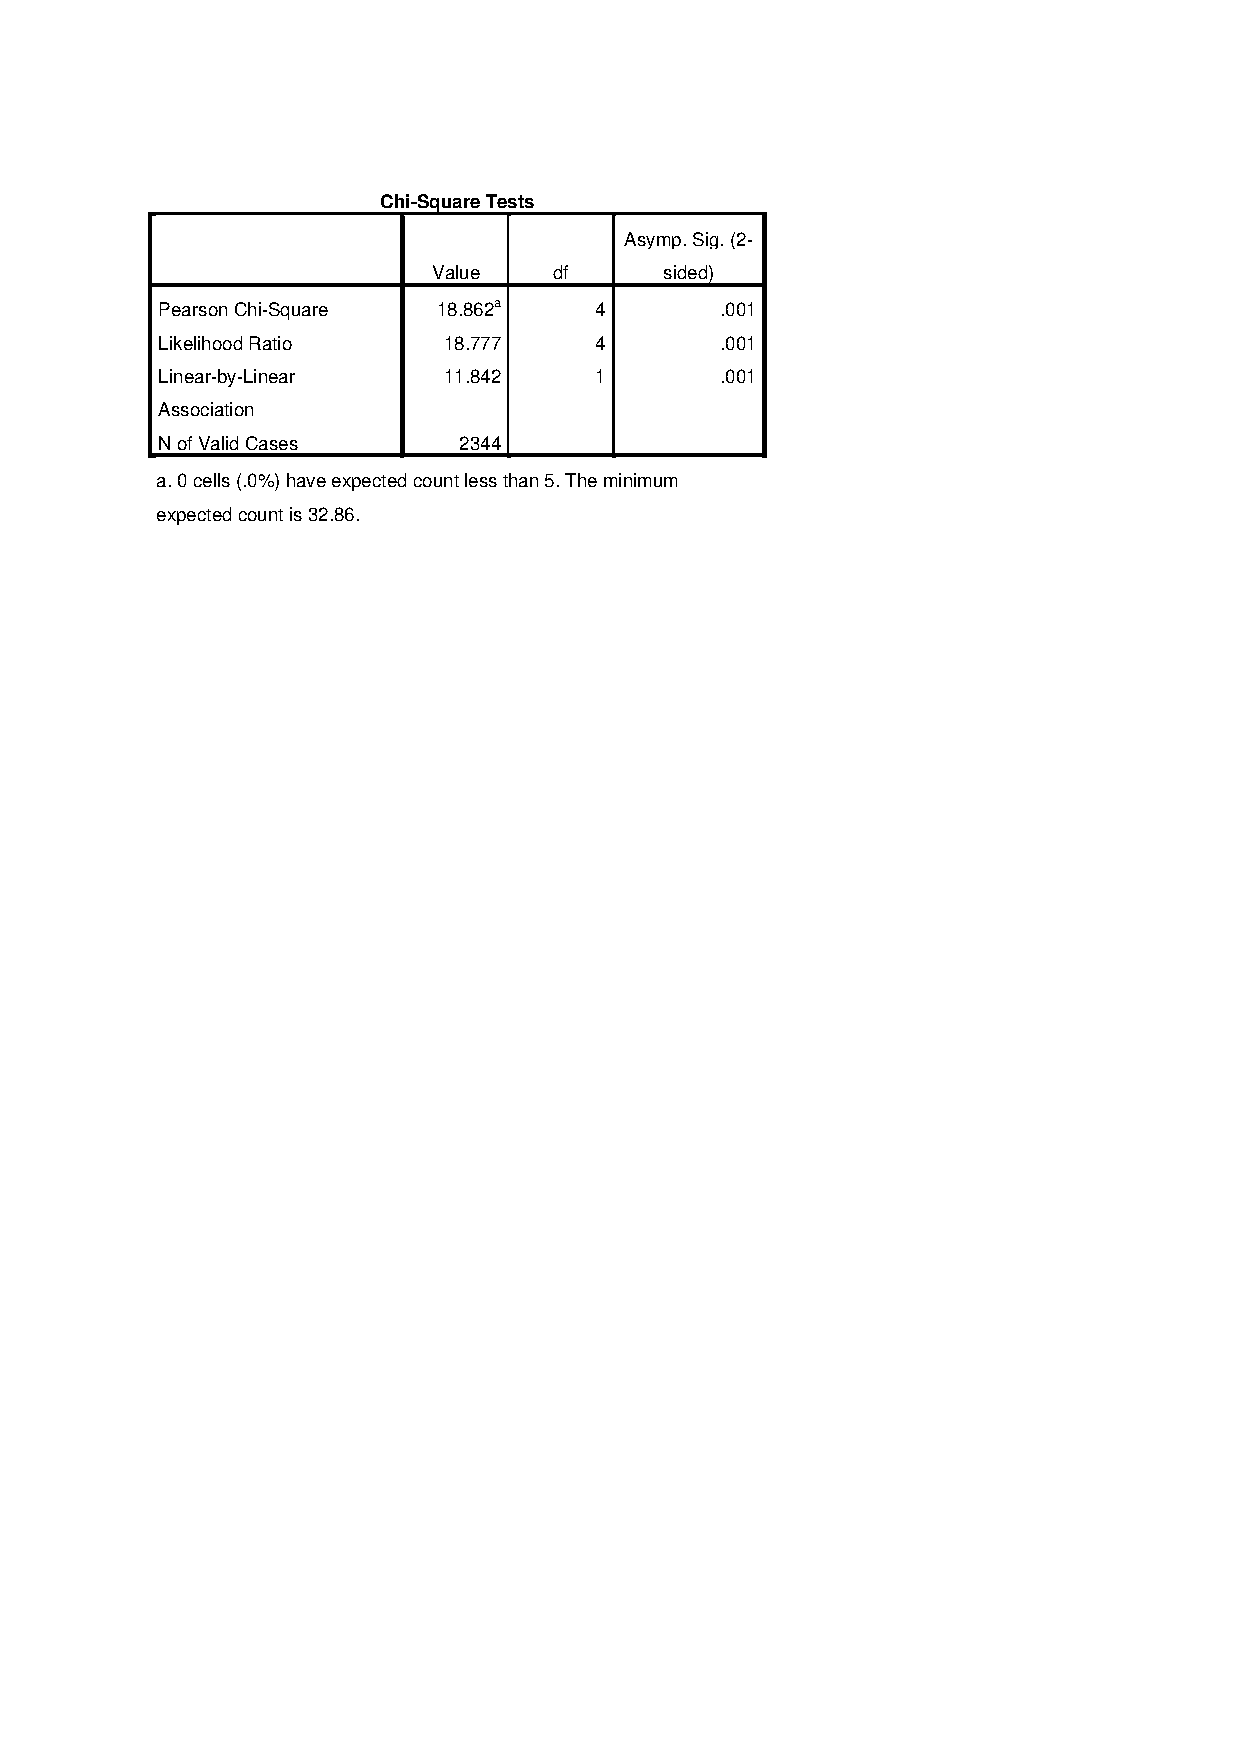
\includegraphics[width=10.00000cm]{chi2test_ess.pdf}
\caption{\label{fig:f-spsschi2} SPSS output of the \(\chi^{2}\) test of
independence (here labelled ``Pearson Chi-square'') for the data in
Table \ref{tab:t-sex-attitude-ch4}.}
\end{figure}

When we apply any significance test, we need to be aware of its
\textbf{assumptions}. These are conditions on the data which are not
themselves being tested, but which need to be approximately satisfied
for the conclusions from the test to be valid. Two broad types of such
assumptions are particularly common. The first kind are assumptions
about the measurement levels and population distributions of the
variables. For the \(\chi^{2}\) test of independence these are
relatively mild. The two variables must be categorical variables. They
can have any measurement level, although in most cases this will be
either nominal or ordinal. The test makes no use of the ordering of the
categories, so it effectively treats all variables as if they were
nominal.

The second common class of assumptions are conditions on the sample
size. Many significance tests are appropriate only if this is
sufficiently large. For the \(\chi^{2}\) test, the expected frequencies
\(f_{e}\) (which will be defined below) need to be large enough in
\emph{every cell} of the table. A common rule of thumb is that the test
can be safely used if all expected frequencies are at least 5. Another,
slightly more lenient rule requires only that no more than 20\% of the
expected frequencies are less than 5, and that none are less than 1.
These conditions can easily be checked with the help of SPSS output for
the \(\chi^{2}\) test, as shown in Figure \ref{fig:f-spsschi2}. This
gives information on the number and proportion of expected frequencies
(referred to as ``expected counts'') less than five, and also the size
of the smallest of them. In our example the smallest expected frequency
is about 33, so the sample size condition is easily satisfied.

When the expected frequencies do not satisfy these conditions, the
\(\chi^{2}\) test is not fully valid, and the results should be treated
with caution (the reasons for this will be discussed below). There are
alternative tests which do not rely on these large-sample assumptions,
but they are beyond the scope of this course.

In general, the hypotheses of a test define the questions it can answer,
and its assumptions indicate the types of data it is appropriate for.
Different tests have different hypotheses and assumptions, which need to
be considered in deciding which test is appropriate for a given
analysis. We will introduce a number of different significance tests in
this coursepack, and give guidelines for choosing between them.

\subsection{The test statistic}\label{ss-tables-chi2test-stat}

A \textbf{test statistic} is a number calculated from the sample (i.e.~a
statistic in the sense defined at the beginning of Section
\ref{s-descr1-nums}) which is used to test a null hypothesis. We we will
describe the calculation of the \(\chi^{2}\) test statistic step by
step, using the data in Table \ref{tab:t-sex-attitude-ch4} for
illustration. All of the elements of the test statistic for this example
are shown in Table \ref{tab:t-sex-attitude-chi2}. These elements are

\begin{itemize}
\item
  The \textbf{observed frequencies}, denoted \(f_{o}\), one for each
  cell of the table. These are simply the observed cell counts (compare
  the \(f_{o}\) column of Table \ref{tab:t-sex-attitude-chi2} to the
  counts in Table \ref{tab:t-sex-attitude-ch4}).
\item
  The \textbf{expected frequencies} \(f_{e}\), also one for each cell.
  These are cell counts in a hypothetical table which would show no
  association between the variables. In other words, they represent a
  table for a sample which would exactly agree with the null hypothesis
  of independence in the population. To explain how the expected
  frequencies are calculated, consider the cell in Table
  \ref{tab:t-sex-attitude-ch4} for Male respondents who strongly agree
  with the statement. As discussed above, if the null hypothesis of
  independence is true in the population, then the conditional
  probability of strongly agreeing is the same for both men and women.
  This also implies that it must then be equal to the overall (marginal)
  probability of strongly agreeing. The sample version of this is that
  the proportion who strongly agree should be the same for men as among
  all respondents overall. This overall proportion in Table
  \ref{tab:t-sex-attitude-ch4} is \(366/2344=0.156\). If this proportion
  applied also to the 1027 male respondents, the number of of them who
  strongly agreed would be
  \[f_{e} = \left(\frac{366}{2344}\right)\times 1027 =
  \frac{366\times 1027}{2344}=160.4.\] Here 2344 is the total sample
  size, and 366 and 1027 are the marginal frequencies of strongly
  agreers and male respondents respectively, i.e.~the two marginal
  totals corresponding to the cell (Male, Strongly agree). The same rule
  applies also in general: the expected frequency for any cell in this
  or any other table is calculated as the product of the row and column
  totals corresponding to the cell, divided by the total sample size.
\item
  The difference \(f_{o}-f_{e}\) between observed and expected
  frequencies for each cell. Since \(f_{e}\) are the cell counts in a
  table which exactly agrees with the null hypothesis, the differences
  indicate how closely the counts \(f_{o}\) actually observed agree with
  \(H_{0}\). If the differences are small, the observed data are
  consistent with the null hypothesis, whereas large differences
  indicate evidence against it. The test statistic will be obtained by
  aggregating information about these differences across all the cells
  of the table. This cannot, however, be done by adding up the
  differences themselves, because positive (\(f_{o}\) is larger than
  \(f_{e}\)) and negative (\(f_{o}\) is smaller than \(f_{e}\))
  differences will always exactly cancel each other out (c.f.~their sum
  on the last row of Table \ref{tab:t-sex-attitude-chi2}). Instead, we
  consider\ldots{}
\item
  \ldots{}the squared differences \((f_{o}-f_{e})^{2}\). This removes
  the signs from the differences, so that the squares of positive and
  negative differences which are equally far from zero will be treated
  as equally strong evidence against the null hypothesis.
\item
  Dividing the squared differences by the expected frequencies, i.e.
  \((f_{o}-f_{e})^{2}/f_{e}\). This is an essential but not particularly
  interesting scaling exercise, which expresses the sizes of the squared
  differences relative to the sizes of \(f_{e}\) themselves.
\item
  Finally, aggregating these quantities to get the \(\chi^{2}\) test
  statistic

  \begin{equation}\chi^{2} = \sum \frac{(f_{o}-f_{e})^{2}}{f_{e}}.
  \label{eq:chi2}\end{equation}

  Here the summation sign \(\Sigma\) indicates that \(\chi^{2}\) is
  obtained by adding up the quantities \((f_{o}-f_{e})^{2}/f_{e}\)
  across all the cells of the table.
\end{itemize}

\begin{longtable}[]{@{}lcrrrrr@{}}
\caption{\label{tab:t-sex-attitude-chi2} Calculating the \(\chi^{2}\) test
statistic for Table \ref{tab:t-sex-attitude-ch4}. In the second column,
SA, A, 0, D, and SD are abbreviations for Strongly agree, Agree, Neither
agree nor disagree, Disagree and Strongly disagree
respectively.}\tabularnewline
\toprule
Cell & Cell & \ & \ & \ & \ & \\tabularnewline
Sex & Attitude & \(f_{o}\) & \(f_{e}\) & \(f_{o}-f_{e}\) &
\((f_{o}-f_{e})^{2}\) & \((f_{o}-f_{e})^{2}/f_{e}\)\tabularnewline
Male & SA & 160 & 160.4 & \(-0.4\) & 0.16 & 0.001\tabularnewline
Male & A & 439 & 477.6 & \(-38.6\) & 1489.96 & 3.120\tabularnewline
Male & 0 & 187 & 186.6 & 0.4 & 0.16 & 0.001\tabularnewline
Male & D & 200 & 169.6 & 30.4 & 924.16 & 5.449\tabularnewline
Male & SD & 41 & 32.9 & 8.1 & 65.61 & 1.994\tabularnewline
Female & SA & 206 & 205.6 & 0.4 & 0.16 & 0.001\tabularnewline
Female & A & 651 & 612.4 & 38.6 & 1489.96 & 2.433\tabularnewline
Female & 0 & 239 & 239.4 & \(-0.4\) & 0.16 & 0.001\tabularnewline
Female & D & 187 & 217.4 & \(-30.4\) & 924.16 & 4.251\tabularnewline
Female & SD & 34 & 42.1 & \(-8.1\) & 65.61 & 1.558\tabularnewline
& Sum & 2344 & 2344 & 0 & 4960.1 & \(\chi^{2}=18.81\)\tabularnewline
\bottomrule
\end{longtable}

The calculations can be done even by hand, but we will usually leave
them to a computer. The last column of Table
\ref{tab:t-sex-attitude-chi2} shows that for Table
\ref{tab:t-sex-attitude-ch4} the test statistic is \(\chi^{2}=18.81\)
(which includes some rounding error, the correct value is 18.862). In
the SPSS output in Figure \ref{fig:f-spsschi2}, it is given in the
``Value'' column of the ``Pearson Chi-Square'' row.

\subsection{The sampling distribution of the test
statistic}\label{ss-tables-chi2test-sdist}

We now know that the value of the \(\chi^{2}\) test statistic in the
example is 18.86. But what does that mean? Why is the test statistic
defined as (\ref{eq:chi2}) and not in some other form? And what does the
number mean? Is 18.86 small or large, weak or strong evidence against
the null hypothesis that sex and attitude are independent in the
population?

In general, a test statistic for any null hypothesis should satisfy two
requirements:

\begin{enumerate}
\def\labelenumi{\arabic{enumi}.}
\item
  The value of the test statistic should be small when evidence against
  the null hypothesis is weak, and large when this evidence is strong.
\item
  The sampling distribution of the test statistic should be known and of
  convenient form when the null hypothesis is true.
\end{enumerate}

Taking the first requirement first, consider the form of
(\ref{eq:chi2}). The important part of this are the squared differences
\((f_{o}-f_{e})^{2}\) for each cell of the table. Here the expected
frequencies \(f_{e}\) reveal what the table would look like if the
sample was in perfect agreement with the claim of independence in the
population, while the observed frequencies \(f_{o}\) show what the
observed table actually does look like. If \(f_{o}\) in a cell is close
to \(f_{e}\), the squared difference is small and the cell contributes
only a small addition to the test statistic. If \(f_{o}\) is very
different from \(f_{e}\) --- either much smaller or much larger than it
--- the squared difference and hence the cell's contribution to the test
statistic are large.

Summing the contributions over all the cells, this implies that the
overall value of the test statistic is small when the observed
frequencies are close to the expected frequencies under the null
hypothesis, and large when at least some of the observed frequencies are
far from the expected ones. (Note also that the smallest possible value
of the statistic is 0, obtained when the observed and the expected
frequency are exactly equal in each cell.) It is thus \emph{large}
values of \(\chi^{2}\) which should be regarded as evidence
\emph{against} the null hypothesis, just as required by condition 1
above.

Turning then to condition 2, we first need to explain what is meant by
``sampling distribution of the test statistic \ldots{} when the null
hypothesis is true''. This is really the conceptual crux of significance
testing. Because it is both so important and relatively abstract, we
will introduce the concept of a sampling distribution in some detail,
starting with a general definition and then focusing on the case of test
statistics in general and the \(\chi^{2}\) test in particular.

\subsubsection*{Sampling distribution of statistic: General
definition}\label{sampling-distribution-of-statistic-general-definition}
\addcontentsline{toc}{subsubsection}{Sampling distribution of statistic:
General definition}

The \(\chi^{2}\) test statistic (\ref{eq:chi2}) is a \emph{statistic} as
defined defined at the beginning of Section \ref{s-descr1-nums}, that is
a number calculated from data in a sample. Once we have observed a
sample, the value of a statistic in that sample is known, such as the
18.862 for \(\chi^{2}\) in our example.

However, we also realise that this value would have been different if
the sample had been different, and also that the sample could indeed
have been different because the sampling is a process that involves
randomness. For example, in the actually observed sample in Table
\ref{tab:t-sex-attitude-ch4} we had 200 men who disagreed with the
statement and 41 who strongly disagreed with it. It is easily imaginable
that another random sample of 2344 respondents from the same population
could have given us frequencies of, say, 195 and 46 for these cells
instead. If that had happened, the value of the \(\chi^{2}\) statistic
would have been 19.75 instead of 18.86. Furthermore, it also seems
intuitively plausible that not all such alternative values are equally
likely for samples from a given population. For example, it seems quite
improbable that the population from which the sample in Table
\ref{tab:t-sex-attitude-ch4} was drawn would instead produce a sample
which also had 1027 men and 1317 women but where all the men strongly
disagreed with the statement (which would yield \(\chi^{2}=2210.3\)).

The ideas that different possible samples would give different values of
a sample statistic, and that some such values are more likely than
others, are formalised in the concept of a sampling distribution:

\begin{itemize}
\tightlist
\item
  The \textbf{sampling distribution of a statistic} is the distribution
  of the statistic (i.e.~its possible values and the proportions with
  which they occur) in the set of all possible random samples of the
  same size from the population.
\end{itemize}

To observe a sampling distribution of a statistic, we would thus need to
draw samples from the population over and over again, and calculate the
value of the statistic for each such sample, until we had a good idea of
the proportions with which different values of the statistic appeared in
the samples. This is clearly an entirely hypothetical exercise in most
real examples where we have just one sample of actual data, whereas the
number of possible samples of that size is essentially or actually
infinite. Despite this, statisticians can find out what sampling
distributions would look like, under specific assumptions about the
population. One way to do so is through mathematical derivations.
Another is a \emph{computer simulation} where we use a computer program
to draw a large number of samples from an artificial population,
calculate the value of a statistic for each of them, and examine the
distribution of the statistic across these repeated samples. We will
make use of both of these approaches below.

\subsubsection*{Sampling distribution of a test statistic under the null
hypothesis}\label{sampling-distribution-of-a-test-statistic-under-the-null-hypothesis}
\addcontentsline{toc}{subsubsection}{Sampling distribution of a test
statistic under the null hypothesis}

The sampling distribution of any statistic depends primarily on what the
population is like. For test statistics, note that requirement 2 above
mentioned only the situation where the null hypothesis is true. This is
in fact the central conceptual ingredient of significance testing. The
basic logic of drawing conclusions from such tests is that we consider
what we would expect to see if the null hypothesis was in fact true in
the population, and compare that to what was actually observed in our
sample. The null hypothesis should then be rejected if the observed data
would be surprising (i.e.~unlikely) if the null hypothesis was actually
true, and not rejected if the observed data would not be surprising
under the null hypothesis.

We have already seen that the \(\chi^{2}\) test statistic is in effect a
measure of the discrepancy between what is expected under the null
hypothesis and what is observed in the sample. All test statistics for
any hypotheses have this property in one way or another. What then
remains to be determined is exactly how surprising or otherwise the
observed data are relative to the null hypothesis. A measure of this is
derived from the sampling distribution of the test statistic \emph{under
the null hypothesis}. It is the only sampling distribution that is
needed for carrying out a significance test.

\subsubsection*{\texorpdfstring{Sampling distribution of the
\(\chi^{2}\) test statistic under
independence}{Sampling distribution of the \textbackslash{}chi\^{}\{2\} test statistic under independence}}\label{sampling-distribution-of-the-chi2-test-statistic-under-independence}
\addcontentsline{toc}{subsubsection}{Sampling distribution of the
\(\chi^{2}\) test statistic under independence}

For the \(\chi^{2}\) test, we need the sampling distribution of the test
statistic (\ref{eq:chi2}) under the independence null hypothesis
(\ref{eq:H0-chi2}). To make these ideas a little more concrete, the
upper part of Table \ref{tab:t-sex-attitude-H0pop} shows the
crosstabulation of sex and attitude in our example for a finite
population where the null hypothesis holds. We can see that it does
because the two conditional distributions for attitude, among men and
among women, are the same (this is the only aspect of the distributions
that matters for this demonstration; the exact values of the
probabilities are otherwise irrelevant). These are of course
hypothetical population distributions, as we do not know the true ones.
We also do not claim that this hypothetical population is even close to
the true one. The whole point of this step of hypothesis testing is to
set up a population where the null hypothesis holds as a fixed point of
comparison, to see what samples from such a population would look like
and how they compare with the real sample that we have actually
observed.

\emph{Population (frequencies are in millions of people):}

\begin{longtable}[]{@{}lcccccr@{}}
\caption{\label{tab:t-sex-attitude-H0pop} \emph{``The government should take
measures to reduce differences in income levels''}: Attitude towards
income redistribution by sex (with row proportions in parentheses), in a
hypothetical population of 50 million people where sex and attitude are
independent, and in one random sample from this
population.}\tabularnewline
\toprule
\begin{minipage}[t]{0.05\columnwidth}\raggedright\strut
Sex\strut
\end{minipage} & \begin{minipage}[t]{0.42\columnwidth}\centering\strut
Agree strongly\strut
\end{minipage} & \begin{minipage}[t]{0.06\columnwidth}\centering\strut
Agree\strut
\end{minipage} & \begin{minipage}[t]{0.09\columnwidth}\centering\strut
Neither agree nor disagree\strut
\end{minipage} & \begin{minipage}[t]{0.06\columnwidth}\centering\strut
Disagree\strut
\end{minipage} & \begin{minipage}[t]{0.06\columnwidth}\centering\strut
Disagree strongly\strut
\end{minipage} & \begin{minipage}[t]{0.04\columnwidth}\raggedleft\strut
Total\strut
\end{minipage}\tabularnewline
\begin{minipage}[t]{0.05\columnwidth}\raggedright\strut
Male\strut
\end{minipage} & \begin{minipage}[t]{0.42\columnwidth}\centering\strut
3.744\strut
\end{minipage} & \begin{minipage}[t]{0.06\columnwidth}\centering\strut
11.160\strut
\end{minipage} & \begin{minipage}[t]{0.09\columnwidth}\centering\strut
4.368\strut
\end{minipage} & \begin{minipage}[t]{0.06\columnwidth}\centering\strut
3.960\strut
\end{minipage} & \begin{minipage}[t]{0.06\columnwidth}\centering\strut
0.768\strut
\end{minipage} & \begin{minipage}[t]{0.04\columnwidth}\raggedleft\strut
24.00\strut
\end{minipage}\tabularnewline
\begin{minipage}[t]{0.05\columnwidth}\raggedright\strut
\strut
\end{minipage} & \begin{minipage}[t]{0.42\columnwidth}\centering\strut
(0.156)\strut
\end{minipage} & \begin{minipage}[t]{0.06\columnwidth}\centering\strut
(0.465)\strut
\end{minipage} & \begin{minipage}[t]{0.09\columnwidth}\centering\strut
(0.182)\strut
\end{minipage} & \begin{minipage}[t]{0.06\columnwidth}\centering\strut
(0.165)\strut
\end{minipage} & \begin{minipage}[t]{0.06\columnwidth}\centering\strut
(0.032)\strut
\end{minipage} & \begin{minipage}[t]{0.04\columnwidth}\raggedleft\strut
(1.0)\strut
\end{minipage}\tabularnewline
\begin{minipage}[t]{0.05\columnwidth}\raggedright\strut
Female\strut
\end{minipage} & \begin{minipage}[t]{0.42\columnwidth}\centering\strut
4.056\strut
\end{minipage} & \begin{minipage}[t]{0.06\columnwidth}\centering\strut
12.090\strut
\end{minipage} & \begin{minipage}[t]{0.09\columnwidth}\centering\strut
4.732\strut
\end{minipage} & \begin{minipage}[t]{0.06\columnwidth}\centering\strut
4.290\strut
\end{minipage} & \begin{minipage}[t]{0.06\columnwidth}\centering\strut
0.832\strut
\end{minipage} & \begin{minipage}[t]{0.04\columnwidth}\raggedleft\strut
26.00\strut
\end{minipage}\tabularnewline
\begin{minipage}[t]{0.05\columnwidth}\raggedright\strut
\strut
\end{minipage} & \begin{minipage}[t]{0.42\columnwidth}\centering\strut
(0.156)\strut
\end{minipage} & \begin{minipage}[t]{0.06\columnwidth}\centering\strut
(0.465)\strut
\end{minipage} & \begin{minipage}[t]{0.09\columnwidth}\centering\strut
(0.182)\strut
\end{minipage} & \begin{minipage}[t]{0.06\columnwidth}\centering\strut
(0.165)\strut
\end{minipage} & \begin{minipage}[t]{0.06\columnwidth}\centering\strut
(0.032)\strut
\end{minipage} & \begin{minipage}[t]{0.04\columnwidth}\raggedleft\strut
(1.0)\strut
\end{minipage}\tabularnewline
\begin{minipage}[t]{0.05\columnwidth}\raggedright\strut
Total\strut
\end{minipage} & \begin{minipage}[t]{0.42\columnwidth}\centering\strut
7.800\strut
\end{minipage} & \begin{minipage}[t]{0.06\columnwidth}\centering\strut
23.250\strut
\end{minipage} & \begin{minipage}[t]{0.09\columnwidth}\centering\strut
9.100\strut
\end{minipage} & \begin{minipage}[t]{0.06\columnwidth}\centering\strut
8.250\strut
\end{minipage} & \begin{minipage}[t]{0.06\columnwidth}\centering\strut
1.600\strut
\end{minipage} & \begin{minipage}[t]{0.04\columnwidth}\raggedleft\strut
50\strut
\end{minipage}\tabularnewline
\begin{minipage}[t]{0.05\columnwidth}\raggedright\strut
\strut
\end{minipage} & \begin{minipage}[t]{0.42\columnwidth}\centering\strut
(0.156)\strut
\end{minipage} & \begin{minipage}[t]{0.06\columnwidth}\centering\strut
(0.465)\strut
\end{minipage} & \begin{minipage}[t]{0.09\columnwidth}\centering\strut
(0.182)\strut
\end{minipage} & \begin{minipage}[t]{0.06\columnwidth}\centering\strut
(0.165)\strut
\end{minipage} & \begin{minipage}[t]{0.06\columnwidth}\centering\strut
(0.032)\strut
\end{minipage} & \begin{minipage}[t]{0.04\columnwidth}\raggedleft\strut
(1.0)\strut
\end{minipage}\tabularnewline
\bottomrule
\end{longtable}

\emph{Sample:}

\begin{longtable}[]{@{}lcccccr@{}}
\caption{\label{tab:t-sex-attitude-H0pop}
\(\chi^{2}=2.8445\)}\tabularnewline
\toprule
\begin{minipage}[t]{0.33\columnwidth}\raggedright\strut
Sex\strut
\end{minipage} & \begin{minipage}[t]{0.08\columnwidth}\centering\strut
Agree strongly\strut
\end{minipage} & \begin{minipage}[t]{0.07\columnwidth}\centering\strut
Agree\strut
\end{minipage} & \begin{minipage}[t]{0.11\columnwidth}\centering\strut
Neither agree nor disagree\strut
\end{minipage} & \begin{minipage}[t]{0.08\columnwidth}\centering\strut
Disagree\strut
\end{minipage} & \begin{minipage}[t]{0.08\columnwidth}\centering\strut
Disagree strongly\strut
\end{minipage} & \begin{minipage}[t]{0.05\columnwidth}\raggedleft\strut
Total\strut
\end{minipage}\tabularnewline
\begin{minipage}[t]{0.33\columnwidth}\raggedright\strut
Male\strut
\end{minipage} & \begin{minipage}[t]{0.08\columnwidth}\centering\strut
181\strut
\end{minipage} & \begin{minipage}[t]{0.07\columnwidth}\centering\strut
505\strut
\end{minipage} & \begin{minipage}[t]{0.11\columnwidth}\centering\strut
191\strut
\end{minipage} & \begin{minipage}[t]{0.08\columnwidth}\centering\strut
203\strut
\end{minipage} & \begin{minipage}[t]{0.08\columnwidth}\centering\strut
41\strut
\end{minipage} & \begin{minipage}[t]{0.05\columnwidth}\raggedleft\strut
1121\strut
\end{minipage}\tabularnewline
\begin{minipage}[t]{0.33\columnwidth}\raggedright\strut
\strut
\end{minipage} & \begin{minipage}[t]{0.08\columnwidth}\centering\strut
(0.161)\strut
\end{minipage} & \begin{minipage}[t]{0.07\columnwidth}\centering\strut
(0.450)\strut
\end{minipage} & \begin{minipage}[t]{0.11\columnwidth}\centering\strut
(0.170)\strut
\end{minipage} & \begin{minipage}[t]{0.08\columnwidth}\centering\strut
(0.181)\strut
\end{minipage} & \begin{minipage}[t]{0.08\columnwidth}\centering\strut
(0.037)\strut
\end{minipage} & \begin{minipage}[t]{0.05\columnwidth}\raggedleft\strut
(1.0)\strut
\end{minipage}\tabularnewline
\begin{minipage}[t]{0.33\columnwidth}\raggedright\strut
Female\strut
\end{minipage} & \begin{minipage}[t]{0.08\columnwidth}\centering\strut
183\strut
\end{minipage} & \begin{minipage}[t]{0.07\columnwidth}\centering\strut
569\strut
\end{minipage} & \begin{minipage}[t]{0.11\columnwidth}\centering\strut
229\strut
\end{minipage} & \begin{minipage}[t]{0.08\columnwidth}\centering\strut
202\strut
\end{minipage} & \begin{minipage}[t]{0.08\columnwidth}\centering\strut
40\strut
\end{minipage} & \begin{minipage}[t]{0.05\columnwidth}\raggedleft\strut
1223\strut
\end{minipage}\tabularnewline
\begin{minipage}[t]{0.33\columnwidth}\raggedright\strut
\strut
\end{minipage} & \begin{minipage}[t]{0.08\columnwidth}\centering\strut
(0.150)\strut
\end{minipage} & \begin{minipage}[t]{0.07\columnwidth}\centering\strut
(0.465)\strut
\end{minipage} & \begin{minipage}[t]{0.11\columnwidth}\centering\strut
(0.187)\strut
\end{minipage} & \begin{minipage}[t]{0.08\columnwidth}\centering\strut
(0.165)\strut
\end{minipage} & \begin{minipage}[t]{0.08\columnwidth}\centering\strut
(0.033)\strut
\end{minipage} & \begin{minipage}[t]{0.05\columnwidth}\raggedleft\strut
(1.0)\strut
\end{minipage}\tabularnewline
\begin{minipage}[t]{0.33\columnwidth}\raggedright\strut
Total\strut
\end{minipage} & \begin{minipage}[t]{0.08\columnwidth}\centering\strut
364\strut
\end{minipage} & \begin{minipage}[t]{0.07\columnwidth}\centering\strut
1074\strut
\end{minipage} & \begin{minipage}[t]{0.11\columnwidth}\centering\strut
420\strut
\end{minipage} & \begin{minipage}[t]{0.08\columnwidth}\centering\strut
405\strut
\end{minipage} & \begin{minipage}[t]{0.08\columnwidth}\centering\strut
81\strut
\end{minipage} & \begin{minipage}[t]{0.05\columnwidth}\raggedleft\strut
2344\strut
\end{minipage}\tabularnewline
\begin{minipage}[t]{0.33\columnwidth}\raggedright\strut
\strut
\end{minipage} & \begin{minipage}[t]{0.08\columnwidth}\centering\strut
(0.155)\strut
\end{minipage} & \begin{minipage}[t]{0.07\columnwidth}\centering\strut
(0.458)\strut
\end{minipage} & \begin{minipage}[t]{0.11\columnwidth}\centering\strut
(0.179)\strut
\end{minipage} & \begin{minipage}[t]{0.08\columnwidth}\centering\strut
(0.173)\strut
\end{minipage} & \begin{minipage}[t]{0.08\columnwidth}\centering\strut
(0.035)\strut
\end{minipage} & \begin{minipage}[t]{0.05\columnwidth}\raggedleft\strut
(1.0)\strut
\end{minipage}\tabularnewline
\bottomrule
\end{longtable}

In the example we have a sample of 2344 observations, so to match that
we want to identify the sampling distribution of the \(\chi^{2}\)
statistic in random samples of size 2344 from the population like the
one in the upper part of Table \ref{tab:t-sex-attitude-H0pop}. The lower
part of that table shows one such sample. Even though it comes from a
population where the two variables are independent, the same is not
exactly true in the sample: we can see that the conditional sample
distributions are not the same for men and women. The value of the
\(\chi^{2}\) test statistic for this simulated sample is 2.8445.

Before we proceed with the discussion of the sampling distribution of
the \(\chi^{2}\) statistic, we should note that it will be a
\emph{continuous} probability distribution. In other words, the number
of distinct values that the test statistic can have in different samples
is so large that their distribution is clearly effectively continuous.
This is true even though the two \emph{variables} in the contingency
table are themselves categorical. The two distributions, the population
distribution of the variables and the sampling distribution of a test
statistic, are quite separate entities and need not resemble each other.
We will consider the nature of continuous probability distributions in
more detail in Chapter \ref{c-means}. In this chapter we will discuss
them relatively superficially and only to the extent that is absolutely
necessary.

Figure \ref{fig:f-chisampld} shows what we observe if do a computer
simulation to draw many more samples from the population in Table
\ref{tab:t-sex-attitude-H0pop}. The figure shows the histogram of the
values of the \(\chi^{2}\) test statistic calculated from 100,000 such
samples. We can see, for example, that \(\chi^{2}\) is between 0 and 10
for most of the samples, and larger than that for only a small
proportion of them. In particular, we note already that the value
\(\chi^{2}=18.8\) that was actually observed in the real sample occurs
very rarely if samples are drawn from a population where the null
hypothesis of independence holds.

\begin{figure}[htbp]
\centering
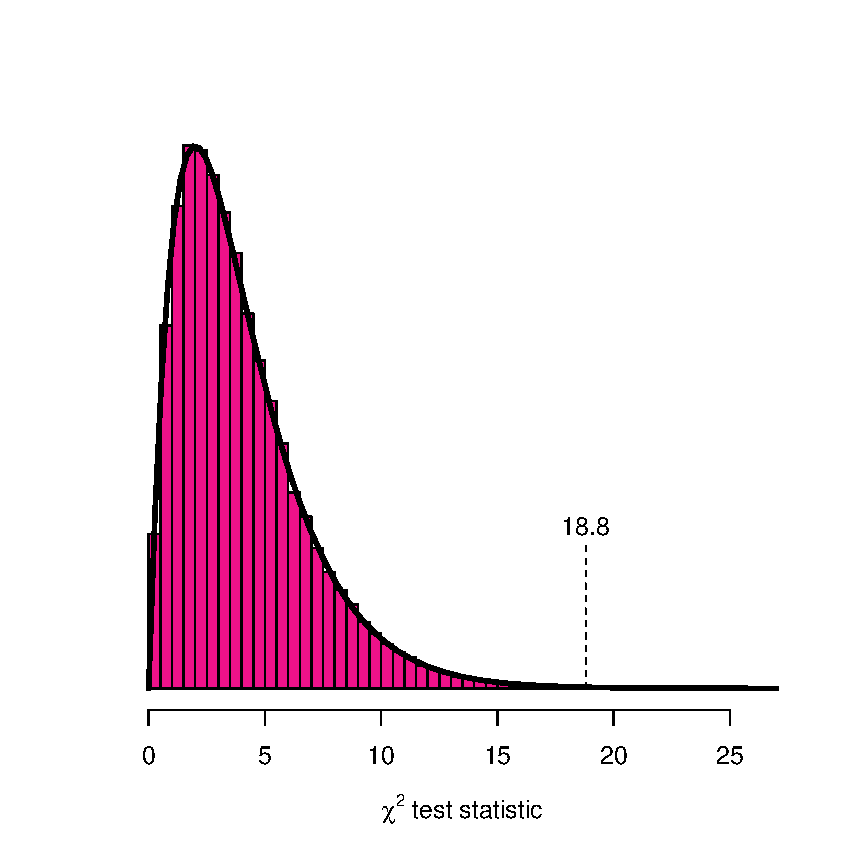
\includegraphics[width=8.50000cm]{chi2sims.pdf}
\caption{\label{fig:f-chisampld} Example of the sampling distribution of the
\(\chi^{2}\) test statistic for independence. The plot shows a histogram
of the values of the statistic in 100,000 simulated samples of size
\(n=2344\) drawn from the population distribution in the upper part of
Table \ref{tab:t-sex-attitude-H0pop}. Superimposed on the histogram is
the curve of the approximate sampling distribution, which is the
\(\chi^{2}\) distribution with 4 degrees of freedom.}
\end{figure}

The form of the sampling distribution can also be derived through
mathematical arguments. These show that for any two-way contingency
table, the approximate sampling distribution of the \(\chi^{2}\)
statistic is a member of a class of continuous probability distributions
known as the \(\boldsymbol{\chi}^{2}\) \textbf{distributions} (the same
symbol \(\chi^{2}\) is rather confusingly used to refer both to the test
statistic and its sampling distribution). The \(\chi^{2}\) distributions
are a family of individual distributions, each of which is identified by
a number known as the \textbf{degrees of freedom} of the distribution.
Figure \ref{fig:f-chi2dists} shows the probability curves of some
\(\chi^{2}\) distributions (what such curves mean is explained in more
detail below, and in Chapter \ref{c-means}). All of the distributions
are skewed to the right, and the shape of a particular curve depends on
its degrees of feedom. All of the curves give non-zero probabilites only
for positive values of the variable on the horizontal axis, indicating
that the value of a \(\chi^{2}\)-distributed variable can never be
negative. This is appropriate for the \(\chi^{2}\) test statistic
(\ref{eq:chi2}), which is also always non-negative.

\begin{figure}[htbp]
\centering
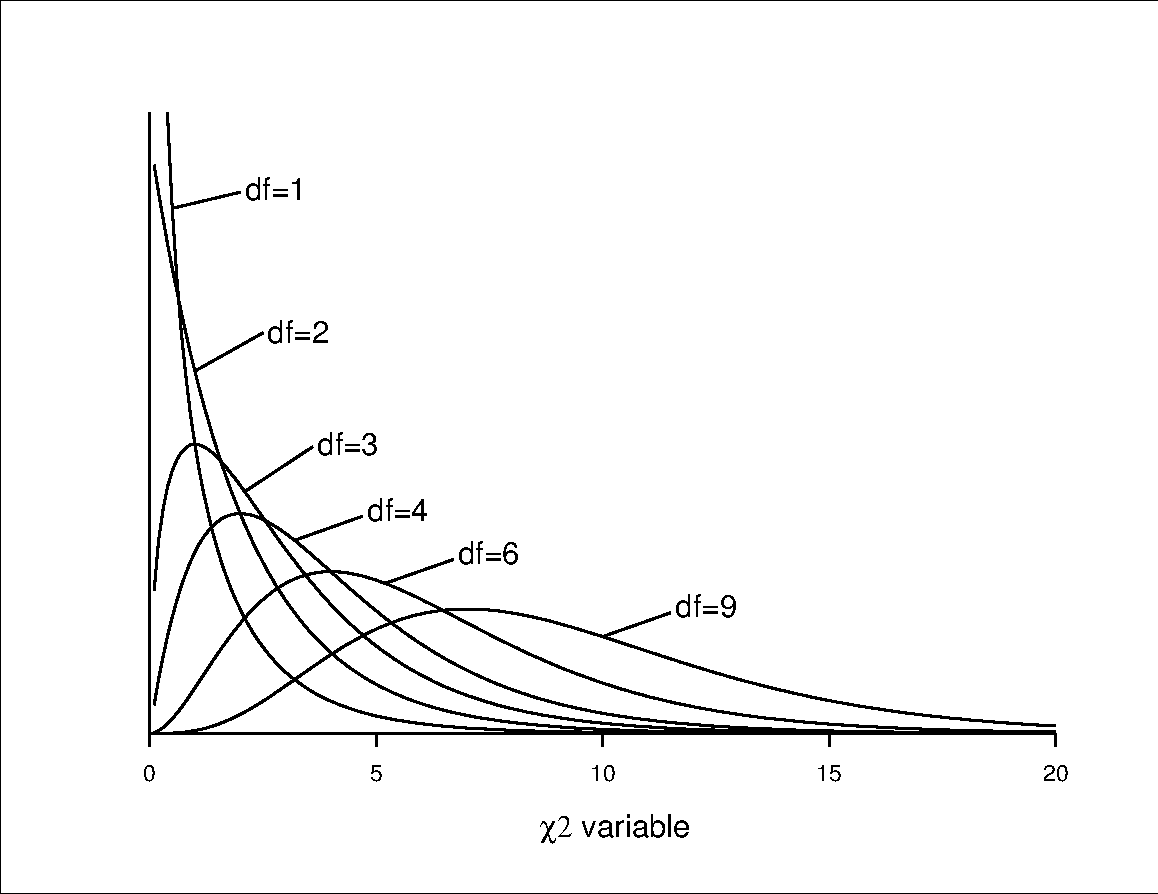
\includegraphics[width=11.50000cm]{chi2dists.pdf}
\caption{\label{fig:f-chi2dists} Probability curves of some \(\chi^{2}\)
distributions with different degrees of freedom (df).}
\end{figure}

For the \(\chi^{2}\) test statistic of independence we have the
following result:

\begin{itemize}
\tightlist
\item
  When the null hypothesis (\ref{eq:H0-chi2}) is true in the population,
  the sampling distribution of the test statistic (\ref{eq:chi2})
  calculated for a two-way table with \(R\) rows and \(C\) columns is
  approximately the \(\chi^{2}\) distribution with \(df=(R-1)(C-1)\)
  degrees of freedom.
\end{itemize}

The degrees of freedom are thus given by the number of rows in the table
minus one, multiplied by the number of columns minus one. Table
\ref{tab:t-sex-attitude-ch4}, for example, has \(R=2\) rows and \(C=5\)
columns, so its degrees of freedom are \(df=(2-1)\times(5-1)=4\) (as
indicated by the ``df'' column of the SPSS output of Figure
\ref{fig:f-spsschi2}). Figure \ref{fig:f-chisampld} shows the curve of
the \(\chi^{2}\) distribution with \(df=4\) superimposed on the
histogram of the sampling distribution obtained from the computer
simulation. The two are in essentially perfect agreement, as
mathematical theory indicates they should be.

These degrees of freedom can be given a further interpretation which
relates to the structure of the table\footnote{The data were obtained
  from
  \url{http://data.london.gov.uk/datastore/package/london-borough-profiles}.

  \noindentIf you download the ``Profiles in Excel'' workbook, you will
  find that one of the pages contains a map of the boroughs, and a tool
  for visualising the data on that map. A regular map of the boroughs
  can be found at for example at

  \url{http://www.londoncouncils.gov.uk/londonfacts/londonlocalgovernment/londonmapandlinks/default.htm}.}.
We can, however, ignore this and treat \(df\) simply as a number which
identifies the appropriate \(\chi^{2}\) distribution to be used for the
\(\chi^{2}\) test for a particular table. Often it is convenient to use
the notation \(\chi^{2}_{df}\) to refer to a specific distribution,
e.g.~\(\chi^{2}_{4}\) for the \(\chi^{2}\) distribution with 4 degrees
of freedom.

The \(\chi^{2}\) sampling distribution is ``approximate'' in that it is
an \emph{asymptotic approximation} which is exactly correct only if the
sample size is infinite and approximately correct when it is
sufficiently large. This is the reason for the conditions for the sizes
of the expected frequencies that were discussed in Section
\ref{ss-tables-chi2test-ass}. When these conditions are satisfied, the
approximation is accurate enough for all practical purposes and we use
the appropriate \(\chi^{2}\) distribution as the sampling distribution.

In Section \ref{ss-tables-chi2test-sdist}, under requirement 2 for a
good test statistic, we mentioned that its sampling distribution under
the null hypothesis should be ``known'' and ``of convenient form''. We
now know that for the \(\chi^{2}\) test it is a \(\chi^{2}\)
distribution. The ``convenient form'' means that the sampling
distribution should not depend on too many specific features of the data
at hand. For the \(\chi^{2}\) test, the approximate sampling
distribution depends (through the degrees of freedom) only on the size
of the table but not on the sample size or the marginal distributions of
the two variables. This is convenient in the right way, because it means
that we can use the same \(\chi^{2}\) distribution for any table with a
given number of rows and columns, as long as the sample size is large
enough for the conditions in Section \ref{ss-tables-chi2test-ass} to be
satisfied.

\subsection{\texorpdfstring{The
\(P\)-value}{The P-value}}\label{ss-tables-chi2test-Pval}

The last key building block of significance testing operationalises the
comparison between the observed value of a test statistic and its
sampling distribution under the null hypothesis. In essence, it provides
a way to determine whether the test statistic in the sample should be
regarded as ``large'' or ``not large'', and with this the measure of
evidence against the null hypothesis that is the end product of the
test:

\begin{itemize}
\tightlist
\item
  The \(\mathbf{P}\)\textbf{-value} is the probability, if the null
  hypothesis was true in the population, of obtaining a value of the
  test statistic which provides as strong or stronger evidence against
  the null hypothesis, and in the direction of the alternative
  hypothesis, as the the value of the test statistic in the sample
  actually observed.
\end{itemize}

The relevance of the phrase ``in the direction of the alternative
hypothesis'' is not apparent for the \(\chi^{2}\) test, so we can ignore
it for the moment. As argued above, for this test it is large values of
the test statistic which indicate evidence against the null hypothesis
of independence, so the values that correspond to ``as strong or
stronger evidence'' against it are the ones that are as large or larger
than the observed statistic. Their probability is evaluated from the
\(\chi^{2}\) sampling distribution defined above.

Figure \ref{fig:f-pvalchisq} illustrates this calculation. It shows the
curve of the \(\chi^{2}_{4}\) distribution, which is the relevant
sampling distribution for the test for the \(2\times 5\) table in our
example. Suppose first, hypothetically, that we had actually observed
the sample in the lower part of Table \ref{tab:t-sex-attitude-H0pop},
for which the value of the test statistic is \(\chi^{2}=2.84\). The
\(P\)-value of the test for this sample would then be the probability of
values of 2.84 or larger, evaluated from the \(\chi^{2}_{4}\)
distribution.

For a probability curve like the one in Figure \ref{fig:f-pvalchisq},
areas under the curve correspond to probabilities. For example, the area
under the whole curve from 0 to infinity is 1, because a variable which
follows the \(\chi^{2}_{4}\) distribution is certain to have one of
these values. Similarly, the probability that we need for the
\(P\)-value for \(\chi^{2}=2.84\) is the area under the curve to the
right of the value 2.84, which is shown in grey in Figure
\ref{fig:f-pvalchisq}. This is \(P=0.585\).

The test statistic for the real sample in Table
\ref{tab:t-sex-attitude-ch4} was \(\chi^{2}=18.86\), so the \(P\)-value
is the combined probability of this and all larger values. This is also
shown in Figure \ref{fig:f-pvalchisq}. However, this area is not really
visible in the plot because 18.86 is far into the tail of the
distribution where the probabilities are low. The \(P\)-value is then
also low, specifically \(P=0.0008\).

\begin{figure}[htbp]
\centering
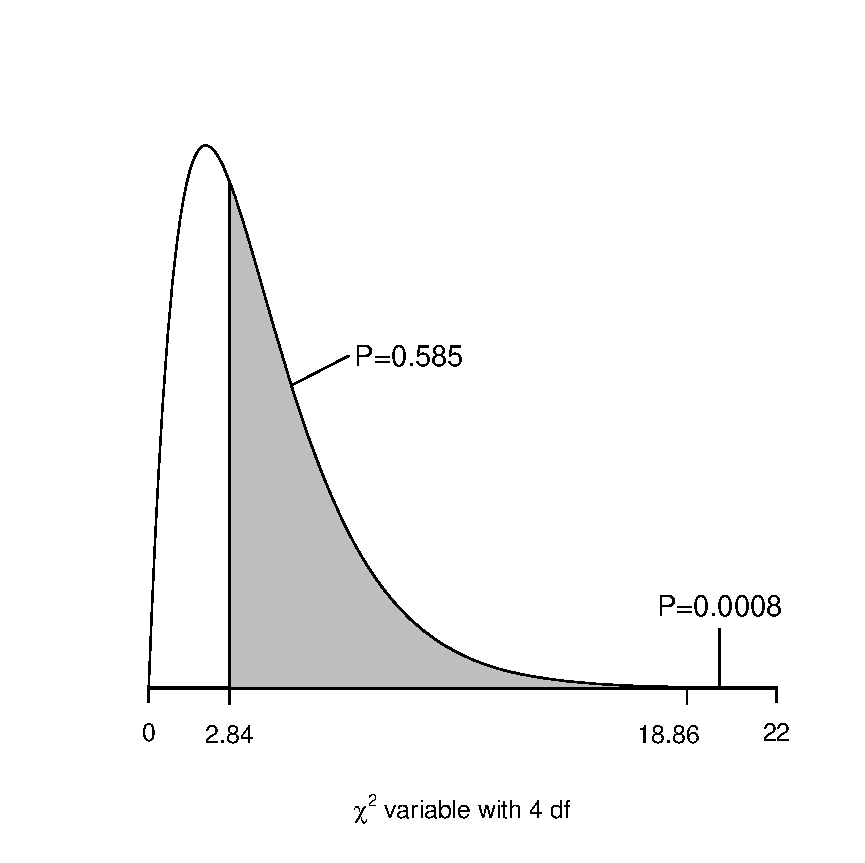
\includegraphics[width=8.00000cm]{chi2_pval.pdf}
\caption{\label{fig:f-pvalchisq} Illustration of the \(P\)-value for a
\(\chi^{2}\) test statistic with 4 degrees of freedom and with values
\(\chi^{2}=2.84\) (area of the grey region under the curve) and
\(\chi^{2}=18.86\).}
\end{figure}

In practice the \(P\)-value is usually calculated by a computer. In the
SPSS output of Figure \ref{fig:f-spsschi2} is is shown in the column
labelled ``Asymp.~Sig. (2-sided)'' which is short for ``Asymptotic
significance level'' (you can ignore the ``2-sided'' for this test). The
value is listed as 0.001. SPSS reports, by default, \(P\)-values rounded
to three decimal places. Sometimes even the smallest of these is zero,
in which case the value is displayed as ``.000''. This is bad practice,
as the \(P\)-value for most significance tests is never \emph{exactly}
zero. \(P\)-values given by SPSS as ``.000'' should be reported instead
as ``\(P<0.001\)''.

Before the widespread availablity of statistical software, \(P\)-values
had to be obtained approximately using tables of distributions. Since
you may still see this approach described in many text books, it is
briefly explained here. You may also need to use the table method in the
examination, where computers are not allowed. Otherwise, however, this
approach is now of little interest: if the \(P\)-value is given in the
computer output, there is no need to refer to distributional tables.

All introductory statistical text books include a table of \(\chi^{2}\)
distributions, although its format may vary slightly form book to book.
Such a table is also included in Section \ref{s-disttables-chi2} of this
coursepack. An extract from the table is shown in Table
\ref{tab:t-chi2table}. Each row of the table corresponds to a
\(\chi^{2}\) distribution with the degrees of freedom given in the first
column. The other columns show so-called ``critical values'' for the
probability levels given on the first row. Consider, for example, the
row for 4 degrees of freedom. The figure 7.78 in the column for
probability level 0.100 indicates that the probability of a value of
7.78 or larger is exactly 0.100 for this distribution. The 9.49 in the
next column shows that the probability of 9.49 or larger is 0.050.
Another way of saying this is that if the appropriate degrees of freedom
were 4, and the test statistic was 7.78, the \(P\)-value would be
exactly 0.100, and if the statistic was 9.49, \(P\) would be 0.050.

\begin{longtable}[]{@{}lrrrr@{}}
\caption{\label{tab:t-chi2table} An extract from a table of critical values
for \(\chi^{2}\) distributions. Row 2-5 show the right-hand tail
probability}\tabularnewline
\toprule
df & 0.100 & 0.050 & 0.010 & 0.001\tabularnewline
1 & 2.71 & 3.84 & 6.63 & 10.83\tabularnewline
2 & 4.61 & 5.99 & 9.21 & 13.82\tabularnewline
3 & 6.25 & 7.81 & 11.34 & 16.27\tabularnewline
4 & 7.78 & 9.49 & 13.28 & 18.47\tabularnewline
\(\vdots\) & \(\vdots\) & & & \(\vdots\)\tabularnewline
\bottomrule
\end{longtable}

The values in the table also provide bounds for other values that are
not shown. For instance, in the hypothetical sample in Table
\ref{tab:t-sex-attitude-H0pop} we had \(\chi^{2}=2.84\), which is
smaller than 7.78. This implies that the corresponding \(P\)-value must
be larger than 0.100, which (of course) agrees with the precise value of
\(P=0.585\) (see also Figure \ref{fig:f-pvalchisq}). Similarly,
\(\chi^{2}=18.86\) for the real data in Table
\ref{tab:t-sex-attitude-ch4}, which is larger than the 18.47 in the
``0.001'' column of the table for the \(\chi^{2}_{4}\) distribution.
Thus the corresponding \(P\)-value must be smaller than 0.001, again
agreeing with the correct value of \(P=0.0008\).

\subsection{Drawing conclusions from a
test}\label{ss-tables-chi2test-conclusions}

The \(P\)-value is the end product of any significance test, in that it
is a complete quantitative summary of the strength of evidence against
the null hypothesis provided by the data in the sample. More precisely,
the \(P\)-value indicates how likely we would be to obtain a value of
the test statistic which was as or more extreme as the value for the
data, if the null hypothesis was true. Thus the \emph{smaller} the
\(P\)-value, the stronger is the evidence \emph{against} the null
hypothesis. For example, in our survey example of sex and attitude
toward income redistribution we obtained \(P=0.0008\) for the
\(\chi^{2}\) test of independence. This is a small number, so it
indicates strong evidence against the claim that the distributions of
attitudes are the same for men and women in the population.

For many purposes it is quite sufficient to simply report the
\(P\)-value. It is, however, quite common also to state the conclusion
in the form of a more discrete decision of ``rejecting'' or ``not
rejecting'' the null hypothesis. This is usually based on conventional
reference levels, known as \textbf{significance levels} or
\(\boldsymbol{\alpha}\)\textbf{-levels} (here \(\alpha\) is the
lower-case Greek letter ``alpha''). The standard significance levels are
0.10, 0.05, 0.01 and 0.001 (also known as 10\%, 5\%, 1\% and 0.1\%
significance levels respectively), of which the 0.05 level is most
commonly used; other values than these are rarely considered. The values
of the test statistic which correspond exactly to these levels are the
critical shown in the table of the \(\chi^{2}\) distribution in Table
\ref{tab:t-chi2table}.

When the \(P\)-value is \emph{smaller} than a conventional level of
significance (i.e.~the test statistic is \emph{larger} than the
corresponding critical value), it is said that the null hypothesis is
\textbf{rejected} at that level of significance, or that the results
(i.e.~evidence against the null hypothesis) are \textbf{statistically
significant} at that level. In our example the \(P\)-value was smaller
than 0.001. The null hypothesis is thus ``rejected at the 0.1 \% level
of significance'', i.e.~the evidence that the variables are not
independent in the population is ``statistically significant at the
0.1\% level'' (as well as the 10\%, 5\% and 1\% levels of course, but it
is enough to state only the strongest level).

The strict decision formulation of significance testing is much overused
and misused. It is in fact quite rare that the statistical analysis will
immediately be followed by some practical action which absolutely
requires a decision about whether to act on the basis of the null
hypothesis or the alternative hypothesis. Typically the analysis which a
test is part of aims to examine some research question, and the results
of the test simply contribute new information to add support for one or
the other side of the argument about the question. The \(P\)-value is
the key measure of the strength and direction of that evidence, so it
should \emph{always} be reported. The standard significance levels used
for rejecting or not rejecting null hypotheses, on the other hand, are
merely useful conventional reference points for structuring the
reporting of test results, and their importance should not be
overemphasised. Clearly \(P\)-values of, say, 0.049 and 0.051 (i.e.~ones
either side of the most common conventional significance level 0.05)
indicate very similar levels of evidence against a null hypothesis, and
acting as if one was somehow qualitatively more decisive is simply
misleading.

\subsubsection*{How to state the
conclusions}\label{how-to-state-the-conclusions}
\addcontentsline{toc}{subsubsection}{How to state the conclusions}

The final step of a significance test is describing its conclusions in a
research report. This should be done with appropriate care:

\begin{itemize}
\item
  The report should make clear which test was used. For example, this
  might be stated as something like ``The \(\chi^{2}\) test of
  independence was used to test the null hypothesis that in the
  population the attitude toward income redistribution was independent
  of sex in the population''. There is usually no need to give
  literature references for the standard tests described on this course.
\item
  The numerical value of the \(P\)-value should be reported, rounded to
  two or three decimal places (e.g.~\(P=0.108\) or \(P=0.11\)). It can
  also reported in an approximate way as, for example, ``\(P<0.05\)''
  (or the same in symbols to save space, e.g.~ for \(P<0.1\), ** for
  \(P<0.05\), and so on). Very small \(P\)-values can always be reported
  as something like ``\(P<0.001\)''.
\item
  When (cautiously) discussing the results in terms of discrete
  decisions, the most common practice is to say that the null hypothesis
  was either \emph{not rejected} or \emph{rejected} at a given
  significance level. It is \emph{not} acceptable to say that the null
  hypothesis was ``accepted'' as an alternative to ``not rejected''.
  Failing to reject the hypothesis that two variables are independent in
  the population is not the same as proving that they actually
  \emph{are} independent.
\item
  A common mistake is to describe the \(P\)-value as the probability
  that the null hypothesis is true. This is understandably tempting, as
  such a claim would seem more natural and convenient than the correct
  but convoluted interpretation of the \(P\)-value as ``the probability
  of obtaining a test statistic as or more extreme as the one observed
  in the data if the test was repeated many times for different samples
  from a population where the null hypothesis was true''. Unfortunately,
  however, the \(P\)-value is \emph{not} the probability of the null
  hypothesis being true. Such a probability does not in fact have any
  real meaning at all in the statistical framework considered
  here\footnote{The data can be obtained from
    \texttt{http://www3.norc.org/gss+website/}, which gives further
    information on the survey, including the full text of the
    questionnaires.}.
\item
  The results of significance tests should be stated using the names and
  values of the variables involved, and not just in terms of ``null''
  and ``alternative'' hypotheses. This also forces you to recall what
  the hypotheses actually were, so that you do not accidentally describe
  the result the wrong way round (e.g.~that the data support a claim
  when they do just the opposite). There are no compulsory phrases for
  stating the conclusions, so it can be done in a number of ways. For
  example, a fairly complete and careful statement in our example would
  be

  \begin{itemize}
  \tightlist
  \item
    ``There is strong evidence that the distributions of attitudes
    toward income redistribution are not the same for men and women in
    the population (\(P<0.001\)).''
  \end{itemize}

  Other possibilities are

  \begin{itemize}
  \item
    ``The association between sex and attitude toward income
    redistribution in the sample is statistically significant
    (\(P<0.001\)).''
  \item
    ``The analysis suggests that there is an association between sex and
    attitude toward income redistribution in the population
    (\(P<0.001\)).''
  \end{itemize}

  The last version is slightly less clear than the other statements in
  that it relies on the reader recognizing that the inclusion of the
  \(P\)-value implies that the word ``differs'' refers to a statistical
  claim rather a statement of absolute fact about the population. In
  many contexts it would be better to say this more explicitly.
\end{itemize}

Finally, if the null hypothesis of independence is rejected, the test
should not usually be the only statistical analysis that is reported for
a two-way table. Instead, we would then go on to describe \emph{how} the
two variables appear to be associated, using the of descriptive methods
discussed in Section \ref{s-descr1-2cat}.

\section{Summary of the chi-square test of
independence}\label{s-tables-summary}

We have now described the elements of a significance test in some
detail. Since it is easy to lose sight of the practical steps of a test
in such a lengthy discussion, they are briefly repeated here for the
\(\chi^{2}\) test of independence. The test of the association between
sex and attitude in the survey example is again used for illustration:

\begin{enumerate}
\def\labelenumi{\arabic{enumi}.}
\item
  Data: observations of two categorical variables, here sex and attitude
  towards income redistribution for \(n=2344\) respondents, presented in
  the two-way, \(2\times 5\) contingency table
  \ref{tab:t-sex-attitude-ch4}.
\item
  Assumptions: the variables can have any measurement level, but the
  expected frequencies \(f_{e}\) must be large enough. A common rule of
  thumb is that \(f_{e}\) should be at least 5 for every cell of the
  table. Here the smallest expected frequency is 32.9, so the
  requirement is comfortably satisfied.
\item
  Hypotheses: null hypothesis \(H_{0}\) that the two variables are
  statistically independent (i.e.~not associated) in the population,
  against the alternative hypothesis that they are dependent.
\item
  The test statistic: the \(\chi^{2}\) statistic \[\chi^{2} = \sum
  \frac{(f_{o}-f_{e})^{2}}{f_{e}}\] where \(f_{o}\) denotes observed
  frequencies in the cells of the table and \(f_{e}\) the corresponding
  expected frequencies under the null hypothesis, and the summation is
  over all of the cells. For Table \ref{tab:t-sex-attitude-ch4},
  \(\chi^{2}=18.86\).
\item
  The sampling distribution of the test statistic when \(H_{0}\) is
  true: a \(\chi^{2}\) distribution with
  \((R-1)\times(C-1)=1\times 4=4\) degrees of freedom, where \(R\)
  \((=2)\) and \(C\) \((=5)\) denote the numbers of rows and columns in
  the table respectively.
\item
  The \(P\)-value: the probability that a randomly selected value from
  the \(\chi^{2}_{4}\) distribution is at least 18.86. This is
  \(P=0.0008\), which may also be reported as \(P<0.001\).
\item
  Conclusion: the null hypothesis of independence is strongly rejected.
  The \(\chi^{2}\) test indicates very strong evidence that sex and
  attitude towards income redistribution are associated in the
  population (\(P<0.001\)).
\end{enumerate}

When the association is judged to be statistically significant, its
nature and magnitude can be further explored using the descriptive
methods for two way tables discussed in Section \ref{s-descr1-2cat}.

\chapter{Inference for population proportions}\label{c-probs}

\section{Introduction}\label{s-probs-intro}

In this chapter we still consider statistical analyses which involve
only discrete, categorical variables. In fact, we now focus on the
simplest case of all, that of \textbf{dichotomous} (binary) variables
which have only two possible values. Four examples which will be used
for illustration throughout this chapter are introduced in Section
\ref{s-probs-examples}. In the first two of them we consider a binary
variable in a single population, while in the last two examples the
question of interest involves a comparison of the distributions of the
variable between two populations (\emph{groups}).

The data for such analyses can be summarised in simple tables, the
one-group case with a one-way table of two cells, and the two-group case
with a \(2\times 2\) contingency table. Here, however, we formulate the
questions of interest slightly differently, with primary emphasis on the
\emph{probability} of one of the two values of the variable of interest.
In the one-group case the questions of interest are then about the
population value of a single probability, and in the two-group case
about the comparison of the values of this probability between the two
groups.

While we describe specific methods of inference for these cases, we also
use them to introduce some further general elements of statistical
inference:

\begin{itemize}
\item
  Population \textbf{parameters} of probability distributions.
\item
  \textbf{Point estimation} of population parameters.
\item
  Hypotheses anout the parameters, and significance tests for them.
\item
  \textbf{Confidence intervals} for population parameters.
\end{itemize}

The comparisons in the two-group analyses again address questions about
associations, now between the group and the dichotomous variable of
interest. Here it will be useful to employ the terminology introduced in
Section \ref{ss-intro-def-assoc}, which distinguishes between the
\textbf{explanatory variable} and the \textbf{response variable} in the
association. Following a common convention, we will denote the
explanatory variable by \(X\) and the response variable by \(Y\). In the
two-group cases of this chapter, \(X\) will be the group (which is
itself also binary) and \(Y\) the binary variable whose probabilities we
are interested in. We will use \(Y\) to denote this binary variable also
in the one-group examples.

\section{Examples}\label{s-probs-examples}

The following four examples will be discussed in this chapter. Examples
5.1 and 5.2 concern only one group, while in Examples 5.3 and 5.4 two
groups are to be compared. Table \ref{tab:t-probex} shows basic sample
statistics for the examples, together with the results of the
significance tests and confidence intervals described later.

\textbf{Example 5.1}: \textbf{An EU referendum}

A referendum about joining the European Union was held in Finland on the
16th of October, 1994. Suppose that in an opinion poll conducted around
October 4th (just before the beginning of postal voting), 330 of the
\(n=702\) respondents (47.0\%) indicated that they would definitely vote
Yes to joining the EU, 190 (27.1\%) said they would definitely vote No,
and 182 (25.9\%) were still undecided\footnote{ESS Round 5: European
  Social Survey Round 5 Data (2010). Data file edition 2.0. Norwegian
  Social Science Data Services, Norway � Data Archive and distributor of
  ESS data. The full data can be obtained from
  \texttt{http://ess.nsd.uib.no/ess/round5/}.}. Here we will consider
the dichotomous variable with the values of Yes (330 respondents) versus
No or Undecided (372 respondents, or 53.0\%). The proportion of voters
who definitely intend to vote Yes provides a lower bound for the
proportion of Yes-votes in the referendum, even if all of the currently
undecided voters eventually decided to vote No.

\textbf{Example 5.2}: \textbf{Evidence of possible racial bias in jury
selection}

As part of an official inquiry into the extent of racial and gender bias
in the justice system in the U.S.~state of Pennsylvania\footnote{The
  data were obtained from
  \url{http://data.london.gov.uk/datastore/package/london-borough-profiles}.

  \noindentIf you download the ``Profiles in Excel'' workbook, you will
  find that one of the pages contains a map of the boroughs, and a tool
  for visualising the data on that map. A regular map of the boroughs
  can be found at for example at

  \url{http://www.londoncouncils.gov.uk/londonfacts/londonlocalgovernment/londonmapandlinks/default.htm}.},
an investigation was made of whether people from minority racial groups
were underrepresented in trial juries. One part of the assessment was a
survey administered to all those called for the jury panel for criminal
trials (from which the juries for actual trials will be selected) in
Allegheny County, Pennsylvania (the city of Pittsburgh and its
surrounding areas) between May and October, 2001. We will consider the
dichotomous variable of whether a respondent to the survey identified
his or her own race as Black (African American) or some other race
category. Of the \(n=4950\) respondents, 226 (4.57\%) identified
themselves as black. This will be compared to the the percentage of
blacks in the whole population of people aged 18 and over (those
eligible for jury service) in the county, which is 12.4\% (this is a
census estimate which will here be treated as a known population
quantity, ignoring any possible census error in it).

\begin{longtable}[]{@{}lrrrrrrr@{}}
\caption{\label{tab:t-probex} Examples of analyses of population proportions
used in Chapter \ref{c-probs}. In addition to sample sizes \(n\) and
proportions \(\hat{\pi}\), the table shows for the one-sample examples
5.1 and 5.2 the \(z\)-test statistic for the hypothesis
\(H_{0}: \pi=\pi_{0}\), its \(P\)-value against a two-sided alternative,
and a 95\% confidence interval for \(\pi\). For the two-sample examples
5.3 and 5.4, the table shows the estimated between-group difference of
proportions \(\hat{\Delta}\), the \(z\)-test statistic for the
hypothesis \(H_{0}: \Delta=0\), its \(P\)-value against a two-sided
alternative, and a 95\% confidence interval for
\(\Delta\).}\tabularnewline
\toprule
\begin{minipage}[b]{0.35\columnwidth}\raggedright\strut
\textbf{One sample}\strut
\end{minipage} & \begin{minipage}[b]{0.05\columnwidth}\raggedleft\strut
\\strut
\end{minipage} & \begin{minipage}[b]{0.04\columnwidth}\raggedleft\strut
\\strut
\end{minipage} & \begin{minipage}[b]{0.06\columnwidth}\raggedleft\strut
\\strut
\end{minipage} & \begin{minipage}[b]{0.11\columnwidth}\raggedleft\strut
\\strut
\end{minipage} & \begin{minipage}[b]{0.05\columnwidth}\raggedleft\strut
\\strut
\end{minipage} & \begin{minipage}[b]{0.05\columnwidth}\raggedleft\strut
\\strut
\end{minipage} & \begin{minipage}[b]{0.07\columnwidth}\raggedleft\strut
\\strut
\end{minipage}\tabularnewline
\midrule
\endfirsthead
\toprule
\begin{minipage}[b]{0.35\columnwidth}\raggedright\strut
\textbf{One sample}\strut
\end{minipage} & \begin{minipage}[b]{0.05\columnwidth}\raggedleft\strut
\\strut
\end{minipage} & \begin{minipage}[b]{0.04\columnwidth}\raggedleft\strut
\\strut
\end{minipage} & \begin{minipage}[b]{0.06\columnwidth}\raggedleft\strut
\\strut
\end{minipage} & \begin{minipage}[b]{0.11\columnwidth}\raggedleft\strut
\\strut
\end{minipage} & \begin{minipage}[b]{0.05\columnwidth}\raggedleft\strut
\\strut
\end{minipage} & \begin{minipage}[b]{0.05\columnwidth}\raggedleft\strut
\\strut
\end{minipage} & \begin{minipage}[b]{0.07\columnwidth}\raggedleft\strut
\\strut
\end{minipage}\tabularnewline
\midrule
\endhead
\begin{minipage}[t]{0.35\columnwidth}\raggedright\strut
Example 5.1: Voting intention in an EU referendum\strut
\end{minipage} & \begin{minipage}[t]{0.05\columnwidth}\raggedleft\strut
\strut
\end{minipage} & \begin{minipage}[t]{0.04\columnwidth}\raggedleft\strut
\strut
\end{minipage} & \begin{minipage}[t]{0.06\columnwidth}\raggedleft\strut
\strut
\end{minipage} & \begin{minipage}[t]{0.11\columnwidth}\raggedleft\strut
\strut
\end{minipage} & \begin{minipage}[t]{0.05\columnwidth}\raggedleft\strut
\strut
\end{minipage} & \begin{minipage}[t]{0.05\columnwidth}\raggedleft\strut
\strut
\end{minipage} & \begin{minipage}[t]{0.07\columnwidth}\raggedleft\strut
\strut
\end{minipage}\tabularnewline
\begin{minipage}[t]{0.35\columnwidth}\raggedright\strut
\strut
\end{minipage} & \begin{minipage}[t]{0.05\columnwidth}\raggedleft\strut
\(n\)\strut
\end{minipage} & \begin{minipage}[t]{0.04\columnwidth}\raggedleft\strut
Yes\strut
\end{minipage} & \begin{minipage}[t]{0.06\columnwidth}\raggedleft\strut
\(\hat{\pi}\)\strut
\end{minipage} & \begin{minipage}[t]{0.11\columnwidth}\raggedleft\strut
\(\pi_{0}\)\strut
\end{minipage} & \begin{minipage}[t]{0.05\columnwidth}\raggedleft\strut
\(z\)\strut
\end{minipage} & \begin{minipage}[t]{0.05\columnwidth}\raggedleft\strut
\(P\)\strut
\end{minipage} & \begin{minipage}[t]{0.07\columnwidth}\raggedleft\strut
95\% CI\strut
\end{minipage}\tabularnewline
\begin{minipage}[t]{0.35\columnwidth}\raggedright\strut
\strut
\end{minipage} & \begin{minipage}[t]{0.05\columnwidth}\raggedleft\strut
702\strut
\end{minipage} & \begin{minipage}[t]{0.04\columnwidth}\raggedleft\strut
330\strut
\end{minipage} & \begin{minipage}[t]{0.06\columnwidth}\raggedleft\strut
0.470\strut
\end{minipage} & \begin{minipage}[t]{0.11\columnwidth}\raggedleft\strut
0.5\strut
\end{minipage} & \begin{minipage}[t]{0.05\columnwidth}\raggedleft\strut
\(-1.59\)\strut
\end{minipage} & \begin{minipage}[t]{0.05\columnwidth}\raggedleft\strut
0.112\strut
\end{minipage} & \begin{minipage}[t]{0.07\columnwidth}\raggedleft\strut
(0.433;\strut
\end{minipage}\tabularnewline
\begin{minipage}[t]{0.35\columnwidth}\raggedright\strut
\strut
\end{minipage} & \begin{minipage}[t]{0.05\columnwidth}\raggedleft\strut
\strut
\end{minipage} & \begin{minipage}[t]{0.04\columnwidth}\raggedleft\strut
\strut
\end{minipage} & \begin{minipage}[t]{0.06\columnwidth}\raggedleft\strut
\strut
\end{minipage} & \begin{minipage}[t]{0.11\columnwidth}\raggedleft\strut
\strut
\end{minipage} & \begin{minipage}[t]{0.05\columnwidth}\raggedleft\strut
\strut
\end{minipage} & \begin{minipage}[t]{0.05\columnwidth}\raggedleft\strut
\strut
\end{minipage} & \begin{minipage}[t]{0.07\columnwidth}\raggedleft\strut
0.507)\strut
\end{minipage}\tabularnewline
\begin{minipage}[t]{0.35\columnwidth}\raggedright\strut
Example 5.2: Race of members of jury panel\strut
\end{minipage} & \begin{minipage}[t]{0.05\columnwidth}\raggedleft\strut
\strut
\end{minipage} & \begin{minipage}[t]{0.04\columnwidth}\raggedleft\strut
\strut
\end{minipage} & \begin{minipage}[t]{0.06\columnwidth}\raggedleft\strut
\strut
\end{minipage} & \begin{minipage}[t]{0.11\columnwidth}\raggedleft\strut
\strut
\end{minipage} & \begin{minipage}[t]{0.05\columnwidth}\raggedleft\strut
\strut
\end{minipage} & \begin{minipage}[t]{0.05\columnwidth}\raggedleft\strut
\strut
\end{minipage} & \begin{minipage}[t]{0.07\columnwidth}\raggedleft\strut
\strut
\end{minipage}\tabularnewline
\begin{minipage}[t]{0.35\columnwidth}\raggedright\strut
\strut
\end{minipage} & \begin{minipage}[t]{0.05\columnwidth}\raggedleft\strut
\(n\)\strut
\end{minipage} & \begin{minipage}[t]{0.04\columnwidth}\raggedleft\strut
Black\strut
\end{minipage} & \begin{minipage}[t]{0.06\columnwidth}\raggedleft\strut
\(\hat{\pi}\)\strut
\end{minipage} & \begin{minipage}[t]{0.11\columnwidth}\raggedleft\strut
\(\pi_{0}\)\strut
\end{minipage} & \begin{minipage}[t]{0.05\columnwidth}\raggedleft\strut
\(z\)\strut
\end{minipage} & \begin{minipage}[t]{0.05\columnwidth}\raggedleft\strut
\(P\)\strut
\end{minipage} & \begin{minipage}[t]{0.07\columnwidth}\raggedleft\strut
95\% CI\strut
\end{minipage}\tabularnewline
\begin{minipage}[t]{0.35\columnwidth}\raggedright\strut
\strut
\end{minipage} & \begin{minipage}[t]{0.05\columnwidth}\raggedleft\strut
4950\strut
\end{minipage} & \begin{minipage}[t]{0.04\columnwidth}\raggedleft\strut
226\strut
\end{minipage} & \begin{minipage}[t]{0.06\columnwidth}\raggedleft\strut
0.0457\strut
\end{minipage} & \begin{minipage}[t]{0.11\columnwidth}\raggedleft\strut
0.124\strut
\end{minipage} & \begin{minipage}[t]{0.05\columnwidth}\raggedleft\strut
\(-16.71\)\strut
\end{minipage} & \begin{minipage}[t]{0.05\columnwidth}\raggedleft\strut
\(<0.001\)\strut
\end{minipage} & \begin{minipage}[t]{0.07\columnwidth}\raggedleft\strut
(0.040;\strut
\end{minipage}\tabularnewline
\begin{minipage}[t]{0.35\columnwidth}\raggedright\strut
\strut
\end{minipage} & \begin{minipage}[t]{0.05\columnwidth}\raggedleft\strut
\strut
\end{minipage} & \begin{minipage}[t]{0.04\columnwidth}\raggedleft\strut
\strut
\end{minipage} & \begin{minipage}[t]{0.06\columnwidth}\raggedleft\strut
\strut
\end{minipage} & \begin{minipage}[t]{0.11\columnwidth}\raggedleft\strut
\strut
\end{minipage} & \begin{minipage}[t]{0.05\columnwidth}\raggedleft\strut
\strut
\end{minipage} & \begin{minipage}[t]{0.05\columnwidth}\raggedleft\strut
\strut
\end{minipage} & \begin{minipage}[t]{0.07\columnwidth}\raggedleft\strut
0.052)\strut
\end{minipage}\tabularnewline
\begin{minipage}[t]{0.35\columnwidth}\raggedright\strut
\textbf{Two Independent samples}\strut
\end{minipage} & \begin{minipage}[t]{0.05\columnwidth}\raggedleft\strut
\strut
\end{minipage} & \begin{minipage}[t]{0.04\columnwidth}\raggedleft\strut
\strut
\end{minipage} & \begin{minipage}[t]{0.06\columnwidth}\raggedleft\strut
\strut
\end{minipage} & \begin{minipage}[t]{0.11\columnwidth}\raggedleft\strut
\strut
\end{minipage} & \begin{minipage}[t]{0.05\columnwidth}\raggedleft\strut
\strut
\end{minipage} & \begin{minipage}[t]{0.05\columnwidth}\raggedleft\strut
\strut
\end{minipage} & \begin{minipage}[t]{0.07\columnwidth}\raggedleft\strut
\strut
\end{minipage}\tabularnewline
\begin{minipage}[t]{0.35\columnwidth}\raggedright\strut
Example 5.3: Polio diagnoses in a vaccine trial\strut
\end{minipage} & \begin{minipage}[t]{0.05\columnwidth}\raggedleft\strut
\strut
\end{minipage} & \begin{minipage}[t]{0.04\columnwidth}\raggedleft\strut
\strut
\end{minipage} & \begin{minipage}[t]{0.06\columnwidth}\raggedleft\strut
\strut
\end{minipage} & \begin{minipage}[t]{0.11\columnwidth}\raggedleft\strut
\strut
\end{minipage} & \begin{minipage}[t]{0.05\columnwidth}\raggedleft\strut
\strut
\end{minipage} & \begin{minipage}[t]{0.05\columnwidth}\raggedleft\strut
\strut
\end{minipage} & \begin{minipage}[t]{0.07\columnwidth}\raggedleft\strut
\strut
\end{minipage}\tabularnewline
\begin{minipage}[t]{0.35\columnwidth}\raggedright\strut
\strut
\end{minipage} & \begin{minipage}[t]{0.05\columnwidth}\raggedleft\strut
\(n\)\strut
\end{minipage} & \begin{minipage}[t]{0.04\columnwidth}\raggedleft\strut
Yes\strut
\end{minipage} & \begin{minipage}[t]{0.06\columnwidth}\raggedleft\strut
\(\hat{\pi}\)\strut
\end{minipage} & \begin{minipage}[t]{0.11\columnwidth}\raggedleft\strut
Diff.~(\(\hat{\Delta}\))\strut
\end{minipage} & \begin{minipage}[t]{0.05\columnwidth}\raggedleft\strut
\(z\)\strut
\end{minipage} & \begin{minipage}[t]{0.05\columnwidth}\raggedleft\strut
\(P\)\strut
\end{minipage} & \begin{minipage}[t]{0.07\columnwidth}\raggedleft\strut
95\% CI\strut
\end{minipage}\tabularnewline
\begin{minipage}[t]{0.35\columnwidth}\raggedright\strut
Control group\strut
\end{minipage} & \begin{minipage}[t]{0.05\columnwidth}\raggedleft\strut
201,229\strut
\end{minipage} & \begin{minipage}[t]{0.04\columnwidth}\raggedleft\strut
142\strut
\end{minipage} & \begin{minipage}[t]{0.06\columnwidth}\raggedleft\strut
0.000706\strut
\end{minipage} & \begin{minipage}[t]{0.11\columnwidth}\raggedleft\strut
\strut
\end{minipage} & \begin{minipage}[t]{0.05\columnwidth}\raggedleft\strut
\strut
\end{minipage} & \begin{minipage}[t]{0.05\columnwidth}\raggedleft\strut
\strut
\end{minipage} & \begin{minipage}[t]{0.07\columnwidth}\raggedleft\strut
\strut
\end{minipage}\tabularnewline
\begin{minipage}[t]{0.35\columnwidth}\raggedright\strut
(placebo)\strut
\end{minipage} & \begin{minipage}[t]{0.05\columnwidth}\raggedleft\strut
\strut
\end{minipage} & \begin{minipage}[t]{0.04\columnwidth}\raggedleft\strut
\strut
\end{minipage} & \begin{minipage}[t]{0.06\columnwidth}\raggedleft\strut
\strut
\end{minipage} & \begin{minipage}[t]{0.11\columnwidth}\raggedleft\strut
\strut
\end{minipage} & \begin{minipage}[t]{0.05\columnwidth}\raggedleft\strut
\strut
\end{minipage} & \begin{minipage}[t]{0.05\columnwidth}\raggedleft\strut
\strut
\end{minipage} & \begin{minipage}[t]{0.07\columnwidth}\raggedleft\strut
\strut
\end{minipage}\tabularnewline
\begin{minipage}[t]{0.35\columnwidth}\raggedright\strut
Treatment group\strut
\end{minipage} & \begin{minipage}[t]{0.05\columnwidth}\raggedleft\strut
200,745\strut
\end{minipage} & \begin{minipage}[t]{0.04\columnwidth}\raggedleft\strut
57\strut
\end{minipage} & \begin{minipage}[t]{0.06\columnwidth}\raggedleft\strut
0.000284\strut
\end{minipage} & \begin{minipage}[t]{0.11\columnwidth}\raggedleft\strut
\(-0.000422\)\strut
\end{minipage} & \begin{minipage}[t]{0.05\columnwidth}\raggedleft\strut
\(-6.01\)\strut
\end{minipage} & \begin{minipage}[t]{0.05\columnwidth}\raggedleft\strut
\(<0.001\)\strut
\end{minipage} & \begin{minipage}[t]{0.07\columnwidth}\raggedleft\strut
\((-0.000560;\)\strut
\end{minipage}\tabularnewline
\begin{minipage}[t]{0.35\columnwidth}\raggedright\strut
(vaccine)\strut
\end{minipage} & \begin{minipage}[t]{0.05\columnwidth}\raggedleft\strut
\strut
\end{minipage} & \begin{minipage}[t]{0.04\columnwidth}\raggedleft\strut
\strut
\end{minipage} & \begin{minipage}[t]{0.06\columnwidth}\raggedleft\strut
\strut
\end{minipage} & \begin{minipage}[t]{0.11\columnwidth}\raggedleft\strut
\strut
\end{minipage} & \begin{minipage}[t]{0.05\columnwidth}\raggedleft\strut
\strut
\end{minipage} & \begin{minipage}[t]{0.05\columnwidth}\raggedleft\strut
\strut
\end{minipage} & \begin{minipage}[t]{0.07\columnwidth}\raggedleft\strut
\(-0.000284)\)\strut
\end{minipage}\tabularnewline
\begin{minipage}[t]{0.35\columnwidth}\raggedright\strut
Example 5.4: Optimistic about young people's future\strut
\end{minipage} & \begin{minipage}[t]{0.05\columnwidth}\raggedleft\strut
\strut
\end{minipage} & \begin{minipage}[t]{0.04\columnwidth}\raggedleft\strut
\strut
\end{minipage} & \begin{minipage}[t]{0.06\columnwidth}\raggedleft\strut
\strut
\end{minipage} & \begin{minipage}[t]{0.11\columnwidth}\raggedleft\strut
\strut
\end{minipage} & \begin{minipage}[t]{0.05\columnwidth}\raggedleft\strut
\strut
\end{minipage} & \begin{minipage}[t]{0.05\columnwidth}\raggedleft\strut
\strut
\end{minipage} & \begin{minipage}[t]{0.07\columnwidth}\raggedleft\strut
\strut
\end{minipage}\tabularnewline
\begin{minipage}[t]{0.35\columnwidth}\raggedright\strut
\strut
\end{minipage} & \begin{minipage}[t]{0.05\columnwidth}\raggedleft\strut
\(n\)\strut
\end{minipage} & \begin{minipage}[t]{0.04\columnwidth}\raggedleft\strut
Yes\strut
\end{minipage} & \begin{minipage}[t]{0.06\columnwidth}\raggedleft\strut
\(\hat{\pi}\)\strut
\end{minipage} & \begin{minipage}[t]{0.11\columnwidth}\raggedleft\strut
Diff.~(\(\hat{\Delta}\))\strut
\end{minipage} & \begin{minipage}[t]{0.05\columnwidth}\raggedleft\strut
\(z\)\strut
\end{minipage} & \begin{minipage}[t]{0.05\columnwidth}\raggedleft\strut
\(P\)\strut
\end{minipage} & \begin{minipage}[t]{0.07\columnwidth}\raggedleft\strut
95\% CI\strut
\end{minipage}\tabularnewline
\begin{minipage}[t]{0.35\columnwidth}\raggedright\strut
Negative question\strut
\end{minipage} & \begin{minipage}[t]{0.05\columnwidth}\raggedleft\strut
921\strut
\end{minipage} & \begin{minipage}[t]{0.04\columnwidth}\raggedleft\strut
257\strut
\end{minipage} & \begin{minipage}[t]{0.06\columnwidth}\raggedleft\strut
0.279\strut
\end{minipage} & \begin{minipage}[t]{0.11\columnwidth}\raggedleft\strut
\strut
\end{minipage} & \begin{minipage}[t]{0.05\columnwidth}\raggedleft\strut
\strut
\end{minipage} & \begin{minipage}[t]{0.05\columnwidth}\raggedleft\strut
\strut
\end{minipage} & \begin{minipage}[t]{0.07\columnwidth}\raggedleft\strut
\strut
\end{minipage}\tabularnewline
\begin{minipage}[t]{0.35\columnwidth}\raggedright\strut
Positive question\strut
\end{minipage} & \begin{minipage}[t]{0.05\columnwidth}\raggedleft\strut
929\strut
\end{minipage} & \begin{minipage}[t]{0.04\columnwidth}\raggedleft\strut
338\strut
\end{minipage} & \begin{minipage}[t]{0.06\columnwidth}\raggedleft\strut
0.364\strut
\end{minipage} & \begin{minipage}[t]{0.11\columnwidth}\raggedleft\strut
0.085\strut
\end{minipage} & \begin{minipage}[t]{0.05\columnwidth}\raggedleft\strut
3.92\strut
\end{minipage} & \begin{minipage}[t]{0.05\columnwidth}\raggedleft\strut
\(<0.001\)\strut
\end{minipage} & \begin{minipage}[t]{0.07\columnwidth}\raggedleft\strut
(0.043; 0.127)\strut
\end{minipage}\tabularnewline
\bottomrule
\end{longtable}

\textbf{Example 5.3: The Salk polio vaccine field trial of 1954}

The first large-scale field trials of the ``killed virus'' polio
vaccination developed by Dr.~Jonas Salk were carried out in the U.S. in
1954\footnote{The data can be obtained from
  \texttt{http://www3.norc.org/gss+website/}, which gives further
  information on the survey, including the full text of the
  questionnaires.}. In the randomized, double-blind placebo-control part
of the trial, a sample of schoolchildren were randomly assigned to
receive either three injections of the polio vaccine, or three
injections of a placebo, inert saltwater which was externally
indistinguishable from the real vaccine. The explanatory variable \(X\)
is thus the group (vaccine or ``treatment'' group vs.~placebo or
``control'' group). The response variable \(Y\) is whether the child was
diagnosed with polio during the trial period (yes or no). There were
\(n_{1}=201,229\) children in the control group, and 142 of them were
diagnosed with polio; in the treatment group, there were 57 new polio
cases among \(n_{2}=200,745\) children (in both cases only those
children who received all three injections are included here). The
proportions of cases of polio were thus \(0.000706\) in the control
group and \(0.000284\) in the vaccinated group (i.e.~7.06 and 2.84 cases
per 10,000 subjects, respectively).

\textbf{Example 5.4: Split-ballot experiment on acquiescence bias}

Survey questions often ask whether respondents agree or disagree with
given statements on opinions or attitudes. \emph{Acquiescence bias}
means the tendency of respondents to agree with such statements,
regardless of their contents. If it is present, we will overestimate the
proportion of people holding the opinion corresponding to agreement with
the statement. The data used in this example come from a study which
examined acquiescence bias through a randomized experiment\footnote{ESS
  Round 5: European Social Survey Round 5 Data (2010). Data file edition
  2.0. Norwegian Social Science Data Services, Norway � Data Archive and
  distributor of ESS data. The full data can be obtained from
  \texttt{http://ess.nsd.uib.no/ess/round5/}.}. In a survey carried out
in Kazakhstan, the respondents were presented with a number of attitude
statements, with four response categories: ``Fully agree'', ``Somewhat
agree'', ``Somewhat disagree'', and ``Fully disagree''. Here we combine
the first two and the last two, and consider the resulting dichotomous
variable, with values labelled ``Agree'' and ``Disagree''.

We consider one item from the survey, concerning the respondents'
opinions on the expectations of today's young people. There were two
forms of the question:

\begin{itemize}
\item
  ``A young person today can expect little of the future''
\item
  ``A young person today can expect much of the future''
\end{itemize}

We will call these the ``Negative'' and ``Positive'' question
respectively. Around half of the respondents were randomly assigned to
receive the positive question, and the rest got the negative question.
The explanatory variable \(X\) indicates the type of question, with
Negative and Positive questions coded here as 1 and 2 respectively. The
dichotomous response variable \(Y\) is whether the respondent gave a
response which was optimistic about the future (i.e.~agreed with the
positive or disagreed with the negative question) or a pessimistic
response. The sample sizes and proportions of optimistic responses in
the two groups are reported in Table \ref{tab:t-probex}. The proportion
is higher when the question was worded positively, as we would expect if
there was acquiescence bias. Whether this difference is statistically
significant remains to be determined.

\section{Probability distribution of a dichotomous
variable}\label{s-probs-distribution}

The response variables \(Y\) considered in this section have only two
possible values. It is common to code them as 0 and 1. In our examples,
we will define the values of the variable of interest as follows:

\begin{itemize}
\item
  Example 5.1: 1 if a person says that he or she will definitely vote
  Yes, and 0 if the respondent will vote No or is undecided
\item
  Example 5.2: 1 for black respondents and 0 for all others
\item
  Example 5.3: 1 if a child developed polio, 0 if not
\item
  Example 5.4: 1 if the respondent gave an optimistic response, 0 if not
\end{itemize}

The population distribution of such a variable is completely specified
by one number, the \textbf{probability} that a randomly selected member
of the population will have the value \(Y=1\) rather than 0. It can also
be thought of as the \textbf{proportion} of units in the population with
\(Y=1\); we will use the two terms interchangeably. This probability is
denoted here \(\pi\) (the lower-case Greek letter ``pi''\footnote{Strictly
  speaking, the analysis should incorporate sampling weights (variable
  \emph{DWEIGHT}) to adjust for different sampling probabilities for
  different types of respondents. Here the weights are ignored. Using
  them would not change the main conclusions for these variables.}). The
value of \(\pi\) is between 0 (no-one in the population has \(Y=1\)) and
1 (everyone has \(Y=1\)). Because \(Y\) can have only two possible
values, and the sum of probabilities must be one, the population
probability of \(Y=0\) is \(1-\pi\).

\label{Binomial} The probability distribution which corresponds to this
kind of population distribution is the \emph{Binomial distribution}. For
later use, we note already here that the mean of this distribution is
\(\pi\) and its variance is \(\pi(1-\pi)\).

In Example 5.1, the population is that of eligible voters at the time of
the opinion poll, and \(\pi\) is the probability that a randomly
selected eligible voter definitely intended to vote Yes. In Example 5.2,
\(\pi\) is the probability that a black person living in the county will
be selected to the jury panel. In Example 5.3, \(\pi\) is the
probability (possibly different in the vaccinated and unvaccinated
groups) that a child will develop polio, and in Example 5.4 it is the
probability (which possibly depends on how the question was asked) that
a respondent will give an optimistic answer to the survey question.

The probability \(\pi\) is the \textbf{parameter} of the binomial
distribution. In general, the parameters of a probability distribution
are one or more numbers which fully determine the distribution. For
example, in the analyses of Chapter \ref{c-tables} we considered
conditional distributions of a one variable in a contingency table given
the other variable. Although we did not make use of this terminology
there, these distributions also have their parameters, whcih are the
probabilities of (all but one of) the categories of the response
variable. Another case will be introduced in Chapter \ref{c-means},
where we consider a probability distribution for a continuous variable,
and its parameters.

\section{Point estimation of a population
probability}\label{s-probs-pointest}

Questions and hypotheses about population distributions are usually most
conveniently formulated in terms of the parameters of the distributions.
For a binary variable \(Y\), this means that statistical inference will
be focused on the probability \(\pi\).

The most obvious question about a parameter is ``what is our best guess
of the value of the parameter in the population?'' The answer will be
based on the information in the sample, using some sample statistic as
the best guess or \textbf{estimate} of the population parameter.
Specifically, this is a \textbf{point estimate}, because it is expressed
as a single value or a ``point'', to distinguish it from \emph{interval}
estimates defined later.

We denote a point estimate of \(\pi\) by \(\hat{\pi}\). The ``\$;
\hat{\;} ; \$'' or ``hat'' is often used to denote an estimate of a
parameter indicated by the symbol under the hat; \(\hat{\pi}\) is read
as ``pi-hat''. As \(\pi\) for a binomial distribution is the population
proportion of \(Y=1\), the obvious choice for a point estimate of it is
the \emph{sample} proportion of units with \(Y=1\). If we denote the
\emph{number} of such units by \(m\), the proportion is thus
\(\hat{\pi}=m/n\), i.e.~\(m\) divided by the sample size \(n\). In
Example 5.1, \(m=330\) and \(n=702\), and \(\hat{\pi}=330/702=0.47\).
This and the estimated proportions in the other examples are shown in
Table \ref{tab:t-probex}, in the two-sample examples 5.3 and 5.4
separately for the two groups.

When \(Y\) is coded with values 0 and 1, \(\hat{\pi}\) is also equal to
the sample mean of \(Y\), since

\begin{equation}\bar{Y}=\frac{Y_{1}+Y_{2}+\dots+Y_{n}}{n}=
\frac{0+0+\dots+0+\overbrace{1+1+\dots+1}^{m \text{ ones}}}{n}=
\frac{m}{n}=\hat{\pi}.
\label{eq:pihat-as-ybar}\end{equation}

\section{Significance test of a single
proportion}\label{s-probs-test1sample}

\subsection{Null and alternative
hypotheses}\label{ss-probs-test1sample-hypotheses}

A null hypothesis about a single population probability \(\pi\) is of
the form

\begin{equation}H_{0}:\; \pi=\pi_{0}
\label{eq:H0p}\end{equation}

where \(\pi_{0}\) is a given number which is either of specific interest
or in some other sense a suitable benchmark in a given application. For
example, in the voting example 5.1 we could consider \(\pi_{0}=0.5\),
i.e.~that the referendum was too close to call. In the jury example 5.2
the value of interest would be \(\pi_{0}=0.124\), the proportion of
blacks in the general adult population of the county.

An alternative but equivalent form of (\ref{eq:H0p}) is expressed in
terms of the difference

\begin{equation}\Delta=\pi-\pi_{0}
\label{eq:Dp}\end{equation}

(\(\Delta\) is the upper-case Greek letter ``Delta''). Then
(@\ref{eq:H0p}) can also be written as

\begin{equation}H_{0}: \; \Delta=0,
\label{eq:H0p2}\end{equation}

i.e.~that there is no difference between the true population probability
and the hypothesised value \(\pi_{0}\). This version of the notation
allows us later to draw attention to the similarities between different
analyses in this chapter and in Chapter~\ref{c-means}. In all of these
cases the quantities of interest turn out to be differences of some
kind, and the formulas for test statistics and confidence intervals will
be of essentially the same form.

The alternative hypothesis to the null hypothesis (\ref{eq:H0p2})
requires some further comments, because there are some new possibilities
that did not arise for the \(\chi^{2}\) test of independence in Chapter
\ref{c-tables}. For the difference \(\Delta\), we may consider two basic
kinds of alternative hypotheses. The first is a \textbf{two-sided
alternative hypothesis}

\begin{equation}H_{a}: \; \Delta\ne 0
\label{eq:Hatwo}\end{equation}

(where ``\(\ne\)'' means ``not equal to''). This claims that the true
value of the population difference \(\Delta\) is some unknown value
which is \emph{not} 0 as claimed by the null hypothesis. With a
two-sided \(H_{a}\), sample evidence that the true difference differs
from 0 will be regarded as evidence against the null hypothesis,
irrespective of whether it suggests that \(\Delta\) is actually smaller
or larger than 0 (hence the word ``two-sided''). When
\(\Delta=\pi-\pi_{0}\), this means that we are trying to assess whether
the true probability \(\pi\) is different from the claimed value
\(\pi_{0}\), but without any expectations about whether \(\pi\) might be
smaller or larger than \(\pi_{0}\).

The second main possibility is one of the two \textbf{one-sided
alternative hypotheses}

\begin{equation}
H_{a}:  \Delta> 0\label{eq:Haonegt}\end{equation}

or

\begin{equation}H_{a}:  \Delta < 0
\label{eq:Haonelt}\end{equation}

Such a hypothesis is only interested in values of \(\Delta\) to one side
of 0, either larger or smaller than it. For example, hypothesis
(\ref{eq:Haonegt}) in the referendum example 5.1, with \(\pi_{0}=0.5\),
is \(H_{a}:\; \pi>0.5\), i.e.~that the proportion who intend to vote Yes
is \emph{greater} than one half. Similarly, in the jury example 5.2,
with \(\pi_{0}=0.124\), (\ref{eq:Haonelt}) is the hypothesis
\(H_{a}:\; \pi<0.124\), i.e.~that the probability that an eligible black
person is selected to a jury panel is \emph{smaller} than the proportion
of blacks in the general population.

Whether we choose to consider a one-sided or a two-sided alternative
hypothesis depends largely on the research questions. In general, a
one-sided hypothesis would be used when deviations from the null
hypothesis only in one direction would be interesting and/or surprising.
This draws on background information about the variables. A two-sided
alternative hypothesis is neutral in this respect. Partly for this
reason, two-sided hypotheses are in practice used more often than
one-sided ones. Choosing a two-sided alternative hypothesis is not wrong
even when a one-sided one could also be considered; this will simply
lead to a more cautious (conservative) approach in that it takes
stronger evidence to reject the null hypothesis when the alternative is
two-sided than when it is one-sided. Such conservatism is typically
regarded as a desirable feature in statistical inference (this will be
discussed further in Section \ref{ss-means-tests3-errors}).

The two-sided alternative hypothesis (\ref{eq:Hatwo}) is clearly the
logical opposite of the null hypothesis (\ref{eq:H0p2}): if \(\Delta\)
is not equal to 0, it must be ``not equal'' to 0. So a two-sided
alternative hypothesis must correspond to a ``point'' null hypothesis
(\ref{eq:H0p2}). For a one-sided alternative hypothesis, the same logic
would seem to imply that the null hypothesis should also be one-sided:
for example, \(H_{0}: \; \Delta\le 0\) and \(H_{a}:\; \Delta>0\) would
form such a logical pair. Often such ``one-sided'' null hypothesis is
also closest to our research questions: for example, it would seem more
interesting to try to test the hypothesis that the proportion of
Yes-voters is less than or equal to 0.5 than that it is exactly 0.5. It
turns out, however, that when the alternative hypothesis is, say,
\(H_{a}: \Delta>0\), the test will be the same when the null hypothesis
is \(H_{0}: \; \Delta\le 0\) as when it is \(H_{0}: \Delta= 0\), and
rejecting or not rejecting one of them is equivalent to rejecting or not
rejecting the other. We can thus here always take the null hypothesis to
be technically of the form (\ref{eq:H0p2}), even if we are really
interested in a corresponding ``one-sided'' null hypothesis. It is then
only the alternative hypothesis which is explicitly either two-sided or
one-sided.

\subsection{The test
statistic}\label{ss-probs-test1sample-teststatistic}

The test statistic used to test hypotheses of the form (\ref{eq:H0p}) is
the \textbf{z-test statistic}

\begin{equation}z=
\frac{\hat{\Delta}}{\hat{\sigma}_{\hat{\Delta}}}=
\frac{\text{Estimate of the population difference $\Delta$}}
{\text{Estimated standard error
of the estimate of $\Delta$}}.
\label{eq:ttest-gen}\end{equation}

The statistic is introduced first in this form in order to draw
attention to its generality. Null hypotheses in many ostensibly
different situations can be formulated as hypotheses of the form
(\ref{eq:H0p2}) about population differences of some kind, and each can
be tested with the test statistic (\ref{eq:ttest-gen}). For example, all
of the test statistics discussed in Chapters \ref{c-probs},
\ref{c-means} and \ref{c-regression} of this course pack will be of this
type (but the \(\chi^{2}\) test statistic of Chapter \ref{c-tables} is
not). The principles of the use and interpretation of the test that are
introduced in this section apply almost unchanged also in these other
contexts, and only the exact formulas for calculating \(\hat{\Delta}\)
and \(\hat{\sigma}_{\hat{\Delta}}\) will need to be defined separately
for each of them. In some applications considered in Chapter
\ref{c-means} the test statistic is typically called the \textbf{t-test
statistic} instead of the \(z\)-test statistic, but its basic idea is
still the same.

In (\ref{eq:ttest-gen}), \(\hat{\Delta}\) denotes a sample estimate of
\(\Delta\). For a test of a single proportion, this is

\begin{equation}\hat{\Delta} = \hat{\pi}-\pi_{0},
\label{eq:Dhatp}\end{equation}

i.e.~the difference between the sample proportion and \(\pi_{0}\). This
is the core of the test statistic. Although the forms of the two
statistics seem rather different, (\ref{eq:Dhatp}) contains the
comparison of the observed and expected sample values that was also at
the heart of the \(\chi^{2}\) test statistic (see formula at end of
Section \ref{ss-tables-chi2test-stat}) in Chapter \ref{c-tables}. Here
the ``observed value'' is the sample estimate \(\hat{\pi}\) of the
probability parameter, ``expected value'' is the value \(\pi_{0}\)
claimed for it by the null hypothesis, and
\(\hat{\Delta}=\hat{\pi}-\pi_{0}\) is their difference. (Equivalently,
we could also say that the expected value of \(\Delta=\pi-\pi_{0}\)
under the null hypothesis (\ref{eq:H0p2}) is 0, its observed value is
\(\hat{\Delta}\), and \(\hat{\Delta}=\hat{\Delta}-0\) is their
difference.)

If the null hypothesis was true, we would expect the observed difference
\(\hat{\Delta}\) to be close to 0. If, on the other hand, the true
\(\pi\) was different from \(\pi_{0}\), we would expect the same to be
true of \(\hat{\pi}\) and thus \(\hat{\Delta}\) to be different from 0.
In other words, the difference \(\hat{\Delta}=\hat{\pi}-\pi_{0}\) tends
to be small (close to zero) when the null hypothesis is true, and large
(far from zero) when it is not true, thus satisfying one of the
requirements for a good test statistic that were stated at the beginning
of Section \ref{ss-tables-chi2test-sdist}. (Whether in this we count as
``large'' both large positive and large negative values, or just one or
the other, depends on the form of the alternative hypothesis, as
explained in the next section.)

The \(\hat{\sigma}_{\hat{\Delta}}\) in (\ref{eq:ttest-gen}) denotes an
estimate of the standard deviation of the sampling distribution of
\(\hat{\Delta}\), which is also known as the estimated \textbf{standard
error} of \(\hat{\Delta}\). For the test statistic (\ref{eq:ttest-gen}),
it is evaluated under the null hypothesis. The concept of a standard
error of an estimate will be discussed in more detail in Section
\ref{s-contd-clt}. Its role in the test statistic is to provide an
interpretable scale for the size of \(\hat{\Delta}\), so that the
sampling distribution discussed in the next section will be of a
convenient form.

For a test of the hypothesis (\ref{eq:H0p}) about a single proportion,
the estimated standard error under the null hypothesis is

\begin{equation}\hat{\sigma}_{\hat{\Delta}} = \sqrt{\frac{\pi_{0}(1-\pi_{0})}{n}},
\label{eq:seDhatp}\end{equation}

and the specific formula of the test statistic (\ref{eq:ttest-gen}) is
then

\begin{equation}z=\frac{\hat{\pi}-\pi_{0}}
{\sqrt{\pi_{0}(1-\pi_{0})/n}}.
\label{eq:ztestp}\end{equation}

This is the \textbf{one-sample \(z\)-test statistic for a population
proportion}.

In Example 5.1 we have \(\hat{\pi}=0.47\), \(\pi_{0}=0.5\), and
\(n=702\), so \[z=\frac{\hat{\pi}-\pi_{0}}{\sqrt{\pi_{0}(1-\pi_{0})/n}}=
\frac{0.47-0.50}{\sqrt{0.50\times(1-0.50)/702}}=-1.59.\] Similarly, in
Example 5.2 we have \(\hat{\pi}=0.0457\), \(\pi_{0}=0.124\), \(n=4950\),
and \[z=\frac{0.0457-0.124}{\sqrt{0.124\times(1-0.124)/4950}}
=
\frac{-0.0783}{\sqrt{0.10862/4950}}=-16.71.\] Strangely, SPSS does not
provide a direct way of calculating this value. However, since the
formula (\ref{eq:ztestp}) is very simple, we can easily calculate it
with a pocket calculator, after first using SPSS to find out
\(\hat{\pi}\). This approach will be used in the computer classes.

\subsection{\texorpdfstring{The sampling distribution of the test
statistic and
\(P\)-values}{The sampling distribution of the test statistic and P-values}}\label{ss-probs-test1sample-samplingd}

Like the \(\chi^{2}\) test of Chapter \ref{c-tables}, the \(z\)-test for
a population proportion requires some conditions on the sample size in
order for the approximate sampling distribution of the test statistic to
be appropriate. These depend also on the value of \(\pi\), which we can
estimate by \(\hat{\pi}\). One rule of thumb is that \(n\) should be
larger than 10 divided by \(\pi\) or \(1-\pi\), whichever is smaller.
When \(\pi\) is not very small or very large, e.g.~if it is between 0.3
and 0.7, this essentially amounts to the condition that \(n\) should be
at least 30. In the voting example 5.1, where \(\hat{\pi}=0.47\), the
sample size of \(n=702\) is clearly large enough. In the jury example
5.2, \(\hat{\pi}=0.0457\) is much closer to zero, but since
\(10/0.0457\) is a little over 200, a sample of \(n=4950\) is again
sufficient.

When the sample size is large enough, the sampling distribution of \(z\)
defined by (\ref{eq:ztestp}) is approximately the \textbf{standard
normal distribution}. The probability curve of this distribution is
shown in Figure \ref{fig:f-pval-prob}. For now we just take it as given,
and postpone a general discussion of the normal distribution until
Chapter \ref{c-means}.

\begin{figure}[htbp]
\centering
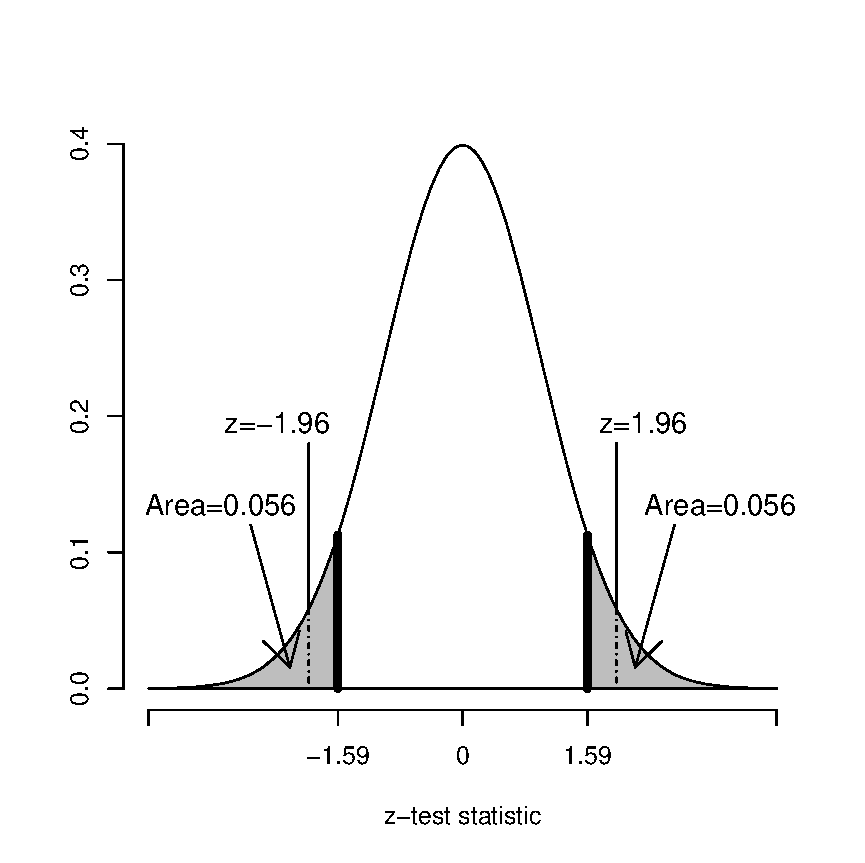
\includegraphics[width=10.00000cm]{pval_zp.pdf}
\caption{\label{fig:f-pval-prob} Illustration of the calculation of
\(P\)-values from the standard normal distribution. Here the value of
the \(z\)-test statistic is \(z=-1.59\) (as in the referendum example
5.1). The areas in grey indicate the two-sided \(P\)-values, i.e.~the
probabilities of values at least as far from 0 as the observed value of
\(z\).}
\end{figure}

The \(P\)-value of the test is calculated from this distribution using
the general principles introduced in Section
\ref{ss-tables-chi2test-Pval}. In other words, the \(P\)-value is the
probability that the test statistic \(z\) has a value that is as or more
extreme than the value of \(z\) in the observed sample. Now, however,
the details of this calculation depend also on the alternative
hypothesis, so some additional explanation is needed.

Consider first the more common case of a two-sided alternative
hypothesis (\ref{eq:Hatwo}), that \(\Delta\ne 0\). As discussed in the
previous section, it is \emph{large} values of the test statistic which
indicate evidence against the null hypothesis, because a large \(z\) is
obtained when the sample difference \(\hat{\Delta}=\hat{\pi}-\pi_{0}\)
is very different from the zero difference claimed by the null
hypothesis. When the alternative is two-sided, ``large'' is taken to
mean any value of \(z\) far from zero, i.e.~either large positive or
large negative values, because both indicate that the sample difference
is far from 0. If \(z\) is large and positive, \(\hat{\Delta}\) is much
\emph{larger} than 0. In example 5.1 this would indicate that a much
larger proportion than 0.5 of the sample say they intend to vote Yes. If
\(z\) is large and negative, \(\hat{\Delta}\) is much \emph{smaller}
than 0, indicating a much smaller sample proportion than 0.5. Both of
these cases would count as evidence against \(H_{0}\) when the
alternative hypothesis is two-sided.

The observed value of the \(z\)-test statistic in Example 5.1 was
actually \(z=-1.59\). Evidence would thus be ``as strong'' against
\(H_{0}\) as the observed \(z\) if we obtained a \(z\)-test statistic of
\(-1.59\) or 1.59, the value exactly as far from 0 as the observed \(z\)
but above rather than below 0. Similarly, evidence against the null
would be even stronger if \(z\) was further from zero than 1.59,
i.e.~larger than 1.59 or smaller than \(-1.59\). To obtain the
\(P\)-value, we thus need to calculate the probability of observing a
\(z\)-test statistic which is at most \(-1.59\) or at least 1.59 when
the null hypothesis is true in the population. In general, the
\(P\)-value for testing the null hypothesis against a two-sided
alternative is the probability of obtaining a value at least \(z\) or at
most \(-z\) (when \(z\) is positive, vice versa when it is negative),
where \(z\) here denotes the value of the test statistic in the sample.
Such probabilities are calculated from the approximately standard normal
sampling distribution of the test statistic under \(H_{0}\).

This calculation of the \(P\)-value is illustrated graphically in Figure
\ref{fig:f-pval-prob}. The curve in the plot is that of the standard
normal distribution. Two areas are shown in grey under the curve, one on
each tail of the distribution. The one on the left corresponds to values
of \(-1.59\) and smaller, and the one on the right to values of 1.59 or
larger. Each of these areas is about 0.056, and the \(P\)-value for a
test against a two-sided alternative is their combined area, i.e.
\(P=0.056+0.056=0.112\). This means that even if the true population
proportion of Yes-voters was actually exactly 0.5, there would be a
probability of 0.112 of obtaining a test statistic as or more extreme
than the \(z=-1.59\) that was actually observed in Example 5.1.

In example 5.2 the observed test statistic was \(z=-16.71\). The
two-sided \(P\)-value is then the probability of values that are at most
\(-16.71\) or at least 16.71. These areas are not shown in Figure
\ref{fig:f-pval-prob} because they would not be visible in it. The
horizontal axis of the figures runs from \(-4\) to \(+4\), so \(-16.71\)
is clearly far in the tail of the distribution and the corresponding
probability is very small; we would report it as \(P<0.001\).

Consider now the case of a one-sided alternative hypothesis. For
example, in the referendum example we might have decided beforehand to
focus only on the possiblity that the proportion of people who intend to
vote Yes is smaller than 0.5, and hence consider the alternative
hypothesis that \(\Delta<0\). Two situations might then arise. First,
suppose that the observed value of the sample difference is in the
direction indicated by the alternative hypothesis. This is the case in
the example, where the sample difference \(\hat{\Delta}=-0.03\) is
indeed smaller than zero, and the test statistic \(t=-1.59\) is
negative. The possible values of \(z\) contributing to the \(P\)-value
are then those of \(-1.59\) or smaller. Values of \(1.59\) and larger
are now not included, because positive values of the test statistic
(corresponding to sample differences greater than 0) would not be
regarded as evidence in favour of the claim that \(\Delta\) is smaller
than 0. The \(P\)-value is thus only the probability corresponding to
the area on the left tail of the curve in Figure \ref{fig:f-pval-prob},
and the corresponding area on the right tail is not included. Since both
areas have the same size, the one-sided \(P\)-value is half the
two-sided value, i.e.~0.056 instead of 0.112. In general, the one-sided
\(P\)-value for a \(z\)-test of a proportion and other similar tests is
always obtained by dividing the two-sided value by 2, if the sample
evidence is in the direction of the one-sided alternative hypothesis.

The second case occurs when the sample difference is not in the
direction indicated by a one-sided alternative hypothesis. For example,
suppose that the sample proportion of Yes-voters had actually been 0.53,
i.e.~0.03 larger than 0.5, so that we had obtained \(z=+1.59\) instead.
The possible values of the test statistic which contributed to the
\(P\)-value would then be \(z=1.59\) and all smaller values. These are
``as strong or stronger evidence against the null hypothesis and in the
direction of the alternative hypothesis'' as required by the definition
at the beginning of Section \ref{ss-tables-chi2test-Pval}, since they
agree with the alternative hypothesis (negative values of \(z\)) or at
least disagree with it less than the observed \(z\) (positive values
from 0 to 1.59). In Figure \ref{fig:f-pval-prob}, these values would
correspond to the area under the whole curve, apart from the region to
the right of \(1.59\) on the right tail. Since the probability of the
latter is 0.056 and the total probability under the curve is 1, the
required probability is \(P=1-0.0.56=0.944\). However, calculating the
\(P\)-value so precisely is hardly necessary in this case, as it is
clearly going to be closer to 1 than to 0. The conclusion from such a
large \(P\)-value will always be that the null hypothesis should not be
rejected. This is also intuitively obvious, as a sample difference in
the opposite direction from the one claimed by the alternative
hypothesis is clearly not to be regarded as evidence in favour of that
alternative hypothesis. In short, if the sample difference is in a
different direction than a one-sided alternative hypothesis, the
\(P\)-value can be reported simply as \(P>0.5\) without further
calculations.

If a statistical software package is used to carry out the test, it will
also report the \(P\)-value and no further calculations are needed
(except dividing a two-sided \(P\)-value by 2, if a one-sided value is
needed and only a two-sided one is reported). However, since SPSS does
not currently provide a procedure for this test, and for exam purposes,
we will briefly outline how an approximate \(P\)-value is obtained using
critical values from a table. This is done in a very similar way as for
the \(\chi^{2}\) test in Section \ref{ss-tables-chi2test-Pval}.

The first part of Table \ref{tab:t-ttable} shows a table of critical
values for the standard normal distribution. These values are also shown
in Section \ref{s-disttables-t} at the end of this course pack, on the
last row of a larger table (the other parts of this table will be
explained later, in Section \ref{ss-means-inference-variants}). A
version of this table is included in all introductory text books on
statistics, although its format may be slightly different in different
books.

\begin{longtable}[]{@{}lrrrrrrr@{}}
\caption{\label{tab:t-ttable} A table of critical values for the standard
normal distribution. The upper part of the table shows the critical
values in one row, as in standard statistical tables (see the last row
of the table in Section \ref{s-disttables-t}). The lower part of the
table includes the same numbers rearranged to show critical values for
conventional significance levels for one- and two-sided
tests.}\tabularnewline
\toprule
& 0.100 & 0.050 & 0.025 & 0.01 & 0.005 & 0.001 & 0.0005\tabularnewline
Critical value & 1.282 & 1.645 & 1.960 & 2.326 & 2.576 & 3.090 &
3.291\tabularnewline
\bottomrule
\end{longtable}

\begin{longtable}[]{@{}lrlll@{}}
\toprule
& Significance levels & & &\tabularnewline
Alternative hypothesis & 0.10 & 0.05 & 0.01 & 0.001\tabularnewline
Two-sided & 1.65 & 1.96 & 2.58 & 3.29\tabularnewline
One-sided & 1.28 & 1.65 & 2.33 & 3.09\tabularnewline
\bottomrule
\end{longtable}

The columns of the first part of Table \ref{tab:t-ttable} are labelled
``Right-hand tail probabilities'', with separate columns for some values
from 0.100 to 0.0005. This means that the probability that a value from
the standard normal distribution is at least as large as the value given
in a particular column is the number given at the top of that column.
For example, the value in the column labelled ``0.025'' is 1.960,
indicating that the probability of obtaining a value equal to or greater
than 1.960 from the standard normal distribution is 0.025. Because the
distribution is symmetric, the probability of values of at most
\(-1.960\) is also 0.025, and the total probability that a value is at
least 1.960 units from zero is \(0.025+0.025=0.05\).

These values can be used to obtain bounds for \(P\)-values, expressed in
terms of conventional significance levels of 0.10, 0.05, 0.01 and 0.001.
The values at which these tail probabilities are obtained are the
corresponding critical values for the test statistic. They are shown in
the lower part of Table \ref{tab:t-ttable}, slightly rearranged for
clarity of presentation and rounded to two decimal places (which is
accurate enough for practical purposes). The basic idea of using the
critical values is that if the observed (absolute value of) the
\(z\)-test statistic is \emph{larger} than a critical value (for the
required kind of alternative hypothesis) shown in the lower part of
Table \ref{tab:t-ttable}, the \(P\)-value is \emph{smaller} than the
significance level corresponding to that critical value.

The table shows only positive critical values. If the observed test
statistic is actually negative, its negative (\(-\)) sign is omitted and
the resulting positive value (i.e.~the absolute value of the statistic)
is compared to the critical values. Note also that the critical value
for a given significance level depends on whether the alternative
hypothesis is two-sided or one-sided. In the one-sided case, the test
statistic is compared to the critical values only if it is actually in
the direction of the alternative hypothesis; if not, we can simply
report \(P>0.5\) as discussed above.

The \(P\)-value obtained from the table is reported as being smaller
than the smallest conventional significance level for which the
corresponding critical value is exceeded by the observed test statistic.
For instance, in the jury example 5.2 we have \(z=-16.71\). Considering
a two-sided alternative hypothesis, 16.71 is larger than the critical
values 1.65, 1.96, 2.58 and 3.29 for all the standard significance
levels, so we can report that \(P<0.001\). For Example 5.1, in contrast,
\(z=-1.59\), the absolute value of which is smaller than even the
critical value 1.65 for the 10\% significance level. For this example,
we would report \(P>0.1\).

The intuitive idea of the critical values and their connection to the
\(P\)-values is illustrated for Example 5.1 by Figure
\ref{fig:f-pval-prob}. Here the observed test statistic is \(t=-1.59\),
so the two-sided \(P\)-value is the probability of values at least 1.59
or at most \(-1.59\), which correspond to the two gray areas in the
tails of the distribution. Also shown in the plot is one of the critical
values for two-sided tests, the 1.96 for significance level 0.05. By
definition of the critical values, the combined tail probability of
values at least 1.96 from 0, i.e.~the probability of values at least
1.96 or at most \(-1.96\), is 0.05. It is clear from the plot that since
1.59 is smaller than 1.96, these areas are smaller than the tail areas
corresponding to 1.59 and \(-1.59\), and the combined area of the latter
must be more than 0.05, i.e.~it must be that \(P>0.05\). Similar
argument for the 10\% critical value of 1.65 shows that \(P\) is here
also larger than 0.1.

\subsection{Conclusions from the
test}\label{ss-probs-test1sample-conclusions}

The general principles of drawing and stating conclusions from a
significance test have already been explained in Section
\ref{ss-tables-chi2test-conclusions}, so they need not be repeated here.
Considering two-sided alternative hypotheses, the conclusions in our two
examples are as follows:

\begin{itemize}
\item
  In the referendum example 5.1, \(P=0.112\) for the null hypothesis
  that \(\pi=0.5\) in the population of eligible voters. The null
  hypothesis is not rejected at conventional levels of significance.
  There is not enough evidence to conclude that the proportion of voters
  who definitely intend to vote Yes differs from one half.
\item
  In the jury example 5.2, \(P<0.001\) for the null hypothesis that
  \(\pi=0.124\). The null hypothesis is thus overwhelmingly rejected at
  any conventional level of significance. There is very strong evidence
  that the probability of a black person being selected to the jury pool
  differs from the proportion of blacks in the population of the county.
\end{itemize}

\subsection{Summary of the test}\label{ss-probs-test1sample-summary}

As a summary, let us again repeat the main steps of the test described
in this section in a concise form, using the voting variable of Example
5.1 for illustration:

\begin{enumerate}
\def\labelenumi{\arabic{enumi}.}
\item
  Data: a sample of size \(n=702\) of a dichotomous variable \(Y\) with
  values 1 (Yes) and 0 (No or undecided), with the sample proportion of
  ones \(\hat{\pi}=0.47\).
\item
  Assumptions: the observations are a random sample from a population
  distribution with some population proportion (probability) \(\pi\),
  and the sample size \(n\) is large enough for the test to be valid
  (for example, \(n\ge 30\) when \(\pi_{0}\) is between about 0.3 and
  0.7, as it is here).
\item
  Hypotheses: null hypothesis \(H_{0}: \pi=\pi_{0}\) against the
  alternative hypothesis \(H_{a}: \pi\ne \pi_{0}\), where
  \(\pi_{0}=0.5\).
\item
  The test statistic: the \(z\)-statistic
  \[z=\frac{\hat{\pi}-\pi_{0}}{\sqrt{\pi_{0}(1-\pi_{0})/n}}=
  \frac{0.47-0.50}{\sqrt{0.50\times(1-0.50)/702}}=-1.59.\]
\item
  The sampling distribution of the test statistic when \(H_{0}\) is
  true: a standard normal distribution.
\item
  The \(P\)-value: the probability that a randomly selected value from
  the the standard normal distribution is at most \(-1.59\) or at least
  1.59, which is \(P=0.112\).

  \begin{itemize}
  \tightlist
  \item
    If the precise \(P\)-value is not available, we can observe that
    1.59 is smaller than the two-sided critical value 1.65 for the 10\%
    level of significance. Thus it must be that \(P>0.1\).
  \end{itemize}
\item
  Conclusion: The null hypothesis is not rejected (\(P=0.112\)). There
  is not enough evidence to conclude that the proportion of eligible
  voters who definitely intend to vote Yes differs from one half. Based
  on this opinion poll, the referendum remains too close to call.
\end{enumerate}

\section{Confidence interval for a single
proportion}\label{s-probs-1sampleci}

\subsection{Introduction}\label{s-probs-1sampleci-intro}

A significance test assesses whether it is plausible, given the evidence
in the observed data, that a population parameter or parameters have a
specific set of values claimed by the null hypothesis. For example, in
Section \ref{s-probs-test1sample} we asked such a question about the
probability parameter of a binary variable in a single population.

In many ways a more natural approach would be try to identify all of
those values of a parameter which \emph{are} plausible given the data.
This leads to a form of statistical inference known as \textbf{interval
estimation}, which aims to present not only a single best guess (i.e.~a
point estimate) of a population parameter, but also a range of plausible
values (an \textbf{interval estimate}) for it. Such an interval is known
as a \textbf{confidence interval}. This section introduces the idea of
confidence intervals, and shows how to construct them for a population
probability. In later sections, the same principles will be used to
calculate confidence intervals for other kinds of population parameters.

Interval estimation is an often underused part of statistical inference,
while significance testing is arguably overused or at least often
misused. In most contexts it would be useful to report confidence
intervals in addition to, or instead of, results of significance tests.
This is not done often enough in research publications in the social
sciences.

\subsection{Calculation of the interval}\label{s-probs-1sampleci-calc}

Our aim is again to draw inference on the difference
\(\Delta=\pi-\pi_{0}\) or, equivalently, the population probability
\(\pi\). The point estimate of \(\Delta\) is
\(\hat{\Delta}=\hat{\pi}-\pi_{0}\) where \(\hat{\pi}\) is the sample
proportion corresponding to \(\pi\). Suppose that the conditions on the
sample size \(n\) that were discussed in Section
\ref{ss-probs-test1sample-samplingd} are again satisfied.

Consider now Figure @ref(fig:f-pval-prob\}. One of the results
illustrated by it is that if \(\pi_{0}\) is the true value of of the
population probability \(\pi\), so that \(\Delta=\pi-\pi_{0}=0\), there
is a probability of 0.95 that for a randomly drawn sample from the
population the \(z\)-test statistic
\(z=\hat{\Delta}/\hat{\sigma}_{\hat{\Delta}}\) is between \(-1.96\) and
\(+1.96\). This also implies that the probability is 0.95 that in such a
sample the observed value of \(\hat{\Delta}\) will be between
\(\Delta-1.96\,\hat{\sigma}_{\hat{\Delta}}\) and
\(\Delta+1.96\,\hat{\sigma}_{\hat{\Delta}}\). Furthermore, it is clear
from the figure that all of the values within this interval are more
likely to occur than any of the values outside the interval (i.e.~those
in the two tails of the sampling distribution). The interval thus seems
like a sensible summary of the ``most likely'' values that the estimate
\(\hat{\Delta}\) may have in random samples.

A confidence interval essentially turns this around, into a statement
about the unknown true value of \(\Delta\) in the population, even in
cases where \(\Delta\) is not 0. This is done by substituting
\(\hat{\Delta}\) for \(\Delta\) above, to create the interval

\begin{equation}\text{from  }
\hat{\Delta} -1.96\times \hat{\sigma}_{\hat{\Delta}}
\text{  to  }
\hat{\Delta}
+1.96\times \hat{\sigma}_{\hat{\Delta}}.
\label{eq:cim0}\end{equation}

This is the \textbf{95 \% confidence interval} for the population
difference \(\Delta\). It is usually written more concisely as

\begin{equation}\hat{\Delta}
\pm 1.96\, \hat{\sigma}_{\hat{\Delta}}
\label{eq:cim1}\end{equation}

where the ``plusminus'' symbol \(\pm\) indicates that we calculate the
two endpoints of the interval as in (\ref{eq:cim0}), one below and one
above \(\hat{\Delta}\).

Expression (\ref{eq:cim1}) is general in the sense that many different
quantities can take the role of \(\Delta\) in it. Here we consider for
now the case of \(\Delta=\pi-\pi_{0}\). The estimated standard error
\(\hat{\sigma}_{\hat{\Delta}}\) is analogous to (\ref{eq:seDhatp}) used
for the \(z\)-test, but not the same. This is because the confidence
interval is not calculated under the null hypothesis
\(H_{0}:\; \pi=\pi_{0}\), so we cannot use \(\pi_{0}\) for \(\pi\) in
the standard error. Instead, \(\pi\) is estimated by the sample
proportion \(\hat{\pi}\), giving the estimated standard error

\begin{equation}\hat{\sigma}_{\hat{\Delta}} = \sqrt{
\frac{\hat{\pi}(1-\hat{\pi})}{n}
}
\label{eq:sephat2}\end{equation}

and thus the 95\% confidence interval \[(\hat{\pi}-\pi_{0}) \pm 1.96 \;
\sqrt{
\frac{\hat{\pi}(1-\hat{\pi})}{n}}\] for \(\Delta=\pi-\pi_{0}\).
Alternatively, a confidence interval for \(\pi\) itself is given by

\begin{equation}\hat{\pi} \pm 1.96 \;
\sqrt{
\frac{\hat{\pi}(1-\hat{\pi})}{n}}.
\label{eq:cip2}\end{equation}

This is typically the most useful interval for use in practice. For
instance, in the referendum example 5.1 this gives a 95\% confidence
interval of
\[0.470\pm 1.96\times \sqrt{\frac{0.470\times(1-0.470)}{702}}
=0.470\pm 0.0369=(0.433, 0.507)\] for the proportion of definite
Yes-voters in the population. Similarly, in Example 5.2 the 95\%
confidence interval for the probability of a black person being selected
for the jury pool is (0.040, 0.052). These intervals are also shown in
Table \ref{tab:t-probex}.

\subsection{Interpretation of confidence
intervals}\label{s-probs-1sampleci-int}

As with the \(P\)-value of a significance test, the precise
interpretation of a confidence interval refers to probabilities
calculated from a sampling distribution, i.e.~probabilities evaluated
from a hypothetical exercise of repeated sampling:

\begin{itemize}
\tightlist
\item
  If we obtained many samples from the population and calculated the
  confidence interval for each such sample using the formula
  (\ref{eq:cip2}), approximately 95\% of these intervals would contain
  the true value of the population proportion \(\pi\).
\end{itemize}

This is undeniably convoluted, even more so than the precise
interpretation of a \(P\)-value. In practise a confidence interval would
not usually be described in exactly these words. Instead, a research
report might, for example, write that (in the referendum example) ``the
95 \% confidence interval for the proportion of eligible voters in the
population who definitely intend to vote Yes is (0.433, 0.507)'', or
that ``we are 95 \% confident that the proportion of eligible voters in
the population who definitely intend to vote Yes is between 43.3\% and
50.7\%''. Such a statement in effect assumes that the readers will be
familiar enough with the idea of confidence intervals to understand the
claim. It is nevertheless useful to be aware of the more careful
interpretation of a confidence interval, if only to avoid
misunderstandings. The most common error is to claim that ``there is a
95\% probability that the proportion in the population is between 0.433
and 0.507''. Although the difference to the interpretation given above
may seem small, the latter statement is not really true, or strictly
speaking even meaningful, in the statistical framework considered here.

In place of the 1.96 in (\ref{eq:cim1}), we may also use other numbers.
To allow for this in the notation, we can also write

\begin{equation}\hat{\Delta} \pm z_{\alpha/2}\; \hat{\sigma}_{\hat{\Delta}}.
\label{eq:ci-D-gen}\end{equation}

where the multiplier \(z_{\alpha/2}\) is a number which depends on two
things. One of them is the sampling distribution of \(\hat{\Delta}\),
which is here assumed to be the normal distribution (another possibility
is discussed in Section \ref{ss-means-inference-variants}). The second
is the \textbf{confidence level} which we have chosen for the confidence
interval. For example, the probability of 0.95 in the interpretation of
a 95\% confidence interval discussed above is the confidence level of
that interval. Conventionally the 0.95 level is most commonly used,
while other standard choices are 0.90 and 0.99, i.e.~90\% and 99\%
confidence intervals.

In the symbol \(z_{\alpha/2}\), \(\alpha\) is a number such that
\(1-\alpha\) equals the required confidence level. In other words,
\(\alpha=0.1\), 0.05, and 0.01 for confidence levels of
\(1-\alpha=0.90\), 0.95 and 0.99 respectively. The values that are
required for the conventional levels are \(z_{0.10/2}=z_{0.05}=1.64\),
\(z_{0.05/2}=z_{0.025}=1.96\), and \(z_{0.01/2}=z_{0.005}=2.58\), which
correspond to intervals at the confidence levels of 90\%, 95\% and 99\%
respectively. These values are also shown in Table \ref{tab:t-ciq}.

\begin{longtable}[]{@{}lrrr@{}}
\caption{\label{tab:t-ciq} Multipliers \(z_{\alpha/2}\) used to obtain
confidence intervals based on the normal distribution, for three
standard confidence levels. These values are substituted for
\(z_{\alpha/2}\) in formula (\ref{eq:ci-D-gen}) to obtain the confidence
interval.}\tabularnewline
\toprule
& Confidence levels & \ & \\tabularnewline
& 90\% & 95\% & 99\%\tabularnewline
Multiplier \(z_{\alpha/2}\) & 1.64 & 1.96 & 2.58\tabularnewline
\bottomrule
\end{longtable}

A confidence interval contains, loosely speaking, those numbers which
are considered plausible values for the unknown population difference
\(\Delta\) in the light of the evidence in the data. The \emph{width} of
the interval thus reflects our uncertainty about the exact value of
\(\Delta\), which in turn is related to the amount of information the
data provide about \(\Delta\). If the interval is wide, many values are
consistent with the observed data, so there is still a large amount of
uncertainty; if the interval is narrow, we have much information about
\(\Delta\) and thus little uncertainty. Another way of stating this is
that when the confidence interval is narrow, estimates of \(\Delta\) are
very \emph{precise}.

The width of the interval (\ref{eq:ci-D-gen}) is
\(2\times z_{\alpha/2}\times \hat{\sigma}_{\hat{\Delta}}\). This depends
on

\begin{itemize}
\item
  The confidence level: the higher the level, the wider the interval.
  Thus a 99\% confidence interval is always wider than a 95\% interval
  for the same data, and wider still than a 90\% interval. This is
  logically inevitable: if we want to state with high level of
  confidence that a parameter is within a certain interval, we must
  allow the interval to contain a wide range of values. It also explains
  why we do not consider a 100\% confidence interval: this would contain
  all possible values of \(\Delta\) and exclude none, making no use of
  the data at all. Instead, we aim for a high but not perfect level of
  confidence, obtaining an interval which contains some but not all
  possible values, for the price of a small chance of incorrect
  conclusions.
\item
  The standard error \(\hat{\sigma}_{\hat{\Delta}}\), which in the case
  of a single proportion is (\ref{eq:sephat2}). This in turn depends on

  \begin{itemize}
  \item
    the sample size \(n\): the larger this is, the narrower the
    interval. Increasing the sample size thus results (other things
    being equal) in reduced uncertainty and higher precision.
  \item
    the true population proportion \(\pi\): the closer this is to 0.5,
    the wider the interval. Unlike the sample size, this determinant of
    the estimation uncertainty is not in our control.
  \end{itemize}
\end{itemize}

Opinion polls of the kind illustrated by the referendum example are
probably where non-academic audiences are most likely to encounter
confidence intervals, although not under that label. Media reports of
such polls typically include a \emph{margin of error} for the results.
For example, in the referendum example it might be reported that 47\% of
the respondents said that they would definitely vote Yes, and that ``the
study has a margin of error of plus or minus four percentage points''.
In most cases the phrase ``margin of error'' refers to a 95\% confidence
interval. Unless otherwise mentioned, we can thus take a statement like
the one above to mean that the 95\% confidence interval for the
proportion of interest is approximately \(47\pm 4\) percentage points.
For a realistic interpretation of the implications of the results, the
width of this interval is at least as important as the point estimate of
the proportion. This is often neglected in media reports of opinion
polls, where the point estimate tends to be headline news, while the
margin of error is typically mentioned only in passing or omitted
altogether.

\subsection{Confidence intervals vs.~significance
tests}\label{ss-means-ci-vstests}

There are some obvious similarities between the conclusions from
significance tests and confidence intervals. For example, a \(z\)-test
in the referendum example 5.1 showed that the null hypothesis that the
population proportion \(\pi\) was 0.5 was not rejected (\(P=0.112\)).
Thus 0.5 is a plausible value for \(\pi\) in light of the observed data.
The 95\% confidence interval for \(\pi\) showed that, at this level of
confidence, plausible values for \(\pi\) are those between 0.433 and
0.507. In particular, these include 0.5, so the confidence interval also
indicates that a proportion of 0.5 is plausible. This connection between
the test and the confidence interval is in fact exact:

\begin{itemize}
\tightlist
\item
  If the hypothesis \(H_{0}: \Delta=0\) about a population quantity
  \(\Delta\) is rejected at the 5\% level of significance using the
  \(z\)-test against a \emph{two-sided} alternative hypothesis, the 95
  \% confidence interval for \(\Delta\) will not contain 0, and vice
  versa. Similarly, if \(H_{0}\) is not rejected, the confidence
  interval will contain 0, and vice versa.
\end{itemize}

The same is true for other matching pairs of levels of significance and
confidence, e.g.~for a test with a 1\% level of significance and a 99\%
(i.e.~(100-1)\%) confidence interval. In short, the significance test
and the confidence interval will in these cases always give the same
answer about whether or not a parameter value is plausible (consistent
with the data) at a given level of significance/confidence.

These pairs of a test and an interval are exactly comparable in that
they concern the same population parameter, estimate all parameters in
the same way, use the same sampling distribution for inference, and use
the same level of significance/confidence. Not all tests and confidence
intervals have exact pairs in this way. Also, some tests are for
hypotheses about more than one parameter at once, so there is no
corresponding single confidence interval. Nevertheless, the connection
stated above is useful for understanding the ideas of both tests and
confidence intervals.

These results also illustrate how confidence intervals are inherently
more informative than significance tests. For instance, in the jury
example 5.2, both the test and the confidence interval agree on the
implausibility of the claim that the population probability of being
selected to the jury panel is the same as the proportion (0.124) of
black people in the population, since the claim that \(\pi=0.124\) is
rejected by the test (with \(P<0.001\)) and outside the interval
\((0.040; 0.052)\). Unlike the test, however, the confidence interval
summarizes the plausibility of \emph{all} possible values of \(\pi\) and
not just \(\pi_{0}=0.124\). One way to describe this is to consider what
would have happened if we had carried out a series of significance tests
of null hypotheses of the form \(H_{0}: \pi=\pi_{0}\) for a range of
values of \(\pi_{0}\). The confidence interval contains all those values
\(\pi_{0}\) which would not have been rejected by the test, while all
the values outside the interval would have been rejected. Here
\(H_{0}: \pi=\pi_{0}\) would thus not have been rejected at the 5\%
level if \(\pi_{0}\) had been between 0.040 and 0.052, and rejected
otherwise. This, of course, is not how significance tests are actually
conducted, but it provides a useful additional interpretation of
confidence intervals.

A confidence interval is particularly useful when the parameter of
interest is measured in familiar units, such as the proportions
considered so far. We may then try to judge, in substantive terms, how
wide the interval is and how far it is from particular values of
interest. In the jury example the 95\% confidence interval ranges from
4.0\% to 5.2\%, which suggests that the population probability is
estimated fairly precisely by this survey. The interval also reveals
that even its upper bound is less than half of the figure of 12.4\%
which would correspond to proportional representation of blacks in the
jury pool, a result which suggests quite substantial underrepresentation
in the pool.

\section{Inference for comparing two
proportions}\label{s-probs-2samples}

In Examples 5.3 and 5.4, the aim is to compare the proportion of a
dichotomous response variable \(Y\) between two groups of a dichotomous
explanatory variable \(X\):

\begin{itemize}
\item
  Example 5.3: compare the proportion of polio cases among the
  unvaccinated (\(\pi_{1}\)) and vaccinated (\(\pi_{2}\)) children.
\item
  Example 5.4: compare the proportion of optimistic responses to a
  negative (\(\pi_{1}\)) vs.~positive wording of the question
  (\(\pi_{2}\)).
\end{itemize}

The quantity of interest is then the population difference

\begin{equation}\Delta=\pi_{2}-\pi_{1}.
\label{eq:Dp2sample}\end{equation}

For a significance test of this, the null hypothesis will again be
\(H_{0}:\; \Delta=0\), which is in this case equivalent to the
hypothesis of equal proportions

\begin{equation}H_{0}:\; \pi_{1} = \pi_{2}.
\label{eq:H0pD}\end{equation}

The null hypothesis thus claims that there is no association between the
group variable \(X\) and the dichotomous response variable \(Y\), while
the alternative hypothesis (e.g.~ the two-sided one
\(H_{a}:\; \pi_{1}\ne \pi_{2}\), i.e.~\(H_{a}:\; \Delta\ne 0\)) implies
that there is an association.

The obvious estimates of \(\pi_{1}\) and \(\pi_{2}\) are the
corresponding sample proportions \(\hat{\pi}_{1}\) and
\(\hat{\pi}_{2}\), calculated from samples of sizes \(n_{1}\) and
\(n_{2}\) respectively, and the estimate of \(\Delta\) is then

\begin{equation}\hat{\Delta}=\hat{\pi}_{2} - \hat{\pi}_{1}.
\label{eq:Dhatpi}\end{equation}

This gives \(\hat{\Delta}=0.000284-0.000706=-0.000422\) in Example 5.3
and \(\hat{\Delta}=0.364-0.279=0.085\) in Example 5.4. In the samples,
the proportion of polio cases is thus lower in the vaccinated group, and
the proportion of optimistic answers is higher in response to a
positively worded question. Note also that although the inference
discussed below focuses on the difference of the proportions, for purely
descriptive purposes we might prefer to use some other statistic, such
as the ratio of the proportions. For example, the difference of 0.000422
in polio incidence between vaccine and control groups may seem small,
because the proportions in both groups are small. A better idea of the
the magnitude of the contrast is given by their ratio of
\(0.000706/0.000284=2.49\) (this is known as the \emph{risk ratio}). In
other words, the rate of polio infection in the unvaccinated group was
two and a half times the rate in the vaccinated group.

\label{p2pthumb} The tests and confidence intervals discussed below are
again based on the assumption that the relevant sampling distributions
are approximately normal, which is true when the sample sizes \(n_{1}\)
and \(n_{2}\) are large enough. The conditions for this are not very
demanding: one rule of thumb states that the methods described in this
section are reasonably valid if in both groups the number of
observations with \(Y\) having the value 1, and of ones with the value
0, are both more than 5. This condition is satisfied in both of the
examples considered here.

The validity of the test, as well as the amount of information the data
provide about \(\pi_{1}\) and \(\pi_{2}\) in general, thus depends not
just on the overall sample sizes but on having enough observations of
both values of \(Y\). The critical quantity is then the number of
observations in the rarer category of \(Y\). In Example 5.3 this means
the numbers of children diagnosed with polio, because the probability of
polio was low in the study population. The numbers of eventual polio
cases were 142 and 57 in the control and treatment groups respectively,
so the rule of thumb stated above was satisfied. With such low
probabilities of polio incidence, sufficient numbers of cases were
achieved only by making the overall sample sizes \(n_{1}\) and \(n_{2}\)
large enough. That is why the trial had to be very large, involving
hundreds of thousands of participants.

The standard error of \(\hat{\Delta}\) is

\begin{equation}\sigma_{\hat{\Delta}} =
\sqrt{
\frac{\pi_{2}(1-\pi_{2})}{n_{2}}
+\frac{\pi_{1}(1-\pi_{1})}{n_{1}}
}.
\label{eq:sigmaDpi}\end{equation}

As in the one-sample case above, the best way to estimate this is
different for a significance test than for a confidence interval. For a
test, the standard error can be estimated under assumption that the null
hypothesis (\ref{eq:H0pD}) is true, in which case the population
proportion is the same in both groups. A good estimate of this common
proportion, denoted below by \(\hat{\pi}\), is the proportion of
observations with value 1 for \(Y\) in the total sample of
\(n_{1}+n_{2}\) observations, pooling observations from both groups
together; expressed in terms of the group-specific estimates, this is

\begin{equation}\hat{\pi} = \frac{n_{1}\hat{\pi}_{1}+n_{2}\hat{\pi}_{2}}{n_{1}+n_{2}}.
\label{eq:phat2sample}\end{equation}

Using this for both \(\pi_{1}\) and \(\pi_{2}\) in (\ref{eq:sigmaDpi})
gives the estimated standard error

\begin{equation}\hat{\sigma}_{\hat{\Delta}}=
\sqrt{
\hat{\pi}(1-\hat{\pi}) \; \left(
\frac{1}{n_{2}}+
\frac{1}{n_{1}}
\right),
}
\label{eq:seDpi}\end{equation}

and using (\ref{eq:Dhatpi}) and (\ref{eq:seDpi}) in the general formula
(\ref{eq:ttest-gen}) gives the \textbf{two-sample \(z\)-test statistic
for proportions}

\begin{equation}z=
\frac{\hat{\pi}_{2}-\hat{\pi}_{1}}
{\sqrt{\hat{\pi}(1-\hat{\pi})(1/n_{2}+1/n_{1})}}
\label{eq:ztestDpi}\end{equation}

where \(\hat{\pi}\) is given by (\ref{eq:phat2sample}). When the null
hypothesis is true, the sampling distribution of this test statistic is
approximately standard normal when the sample sizes are large enough.

For a confidence interval, the calculation of the estimated standard
error cannot assume that (\ref{eq:H0pD}) is true. Instead, we use the
estimate

\begin{equation}\hat{\sigma}_{\hat{\Delta}} =
\sqrt{
\frac{\hat{\pi}_{2}(1-\hat{\pi}_{2})}{n_{2}} +
\frac{\hat{\pi}_{1}(1-\hat{\pi}_{1})}{n_{1}}
}
\label{eq:seDpi2}\end{equation}

and, substituting this to the general formula (\ref{eq:ci-D-gen}), we
get

\begin{equation}(\hat{\pi}_{2}-\hat{\pi}_{1}) \pm z_{\alpha/2} \;
\sqrt{
\frac{\hat{\pi}_{2}(1-\hat{\pi}_{2})}{n_{2}} +
\frac{\hat{\pi}_{1}(1-\hat{\pi}_{1})}{n_{1}}
}
\label{eq:ciDpi}\end{equation}

as the confidence interval for \(\Delta=\pi_{2}-\pi_{1}\), with
confidence level \(1-\alpha\).

For an illustration of the calculations, consider Example 5.4. Denoting
the group of respondents answering the negatively worded question by 1
and those with the positive question by 2, the basic quantities are
\(n_{1}=921\), \(\hat{\pi}_{1}=0.279\), \(n_{2}=929\) and
\(\hat{\pi}_{2}=0.364\). The estimated difference in the proportions of
respondents giving an optimistic answer is thus
\[\hat{\Delta} = \hat{\pi}_{2}-\hat{\pi}_{1} = 0.364-0.279 = 0.085.\]
For a significance test, the estimated standard error of
\(\hat{\Delta}\) uses the pooled estimate (\ref{eq:phat2sample}) of the
population proportion, which is given by
\[\hat{\pi} = \frac{921\times 0.279+929\times 0.364}{921+929}=
\frac{257+338}{921+929} = 0.322.\] The standard error from
(\ref{eq:seDpi}) is then \[\hat{\sigma}_{\hat{\Delta}}
=
\sqrt{
0.322\times(1-0.322) \times \left(
\frac{1}{929}+
\frac{1}{921}
\right)
}
=
\sqrt{
\frac{0.2182}{462.5}
}=0.0217,\] and the test statistic (\ref{eq:ztestDpi}) is
\[z=\frac{0.085}{0.0217}=3.92.\] For the confidence interval, the
standard error of \(\hat{\Delta}\) is estimated from (\ref{eq:seDpi2})
as \[\begin{aligned}
\hat{\sigma}_{\hat{\Delta}} &=&
\sqrt{
\frac{0.364\times (1-0.364)}{929} +
\frac{0.279\times (1-0.279)}{921}
} \\
&=&
\sqrt{
\frac{0.2315}{929}
+\frac{0.2012}{921}
}=0.0216\end{aligned}\] and a 95\% confidence interval from
(\ref{eq:ciDpi}) is
\[0.085 \pm 1.96 \times 0.0216 = 0.085\pm 0.042 = (0.043; 0.127).\] The
\(P\)-value for the test statistic is clearly very low (in fact about
\(0.00009\)), so the null hypothesis of equal proportions is
convincingly rejected. There is very strong evidence that the
probability that a respondent will give an answer indicating optimism
for the future is different for the two differently worded questions.
The confidence interval indicates that we are 95\% confident that the
proportion of optimistic answers is between 4.3 and 12.7 percentage
points higher when the question is worded positively than when it is
worded negatively. This suggests quite a substantial acquiescence bias
arising from changing just one word in the survey question, as described
in the introduction to Example 5.4 at the beginning of this chapter.

In Example 5.3, the estimated difference is \(\hat{\Delta}=-0.000422\)
(see Table \ref{tab:t-probex}, i.e.~422 fewer polio cases per million
children in the vaccinated group than in the unvaccinated group. Similar
calculations as above show that the value of the test statistic is
\(z=-6.01\), so the \(P\)-value is again very small (in fact about
0.000000001) and the null hypothesis of equal probabilities is strongly
rejected. There is thus overwhelming evidence that the proportion of
polio cases was different among the vaccinated children than among the
unvaccinated ones. The 95\% confidence interval for the difference shows
that we are 95\% confident that this difference was a reduction of
between 284 and 560 polio cases per million children\footnote{The data
  can be obtained from \texttt{http://bes2009-10.org/}, which gives
  further information on the survey, including the full text of the
  questionnaires. The data analysed in this class and homework are from
  the BES Campaign Internet Panel Survey, which has been divided into
  two data sets corresponding to two time periods leading up to the
  General Election.}. This was acknowledged as a convincing
demonstration that the Salk vaccine worked (see Figure
\ref{fig:f-nytimes}), and it (and later other types of polio
vaccination) was soon put to widespread use. The resulting dramatic
decline in the incidence of polio is one of the great success stories of
modern medicine. Compared to the 199 children with polio in 1954 among
the less than half a million participants of the vaccine trial alone, in
2014 there were 414 confirmed cases of polio in the whole world (see
\texttt{www.polioeradication.org/Dataandmonitoring/Poliothisweek.aspx}).
There is hope that that number will reach 0 in a not-too-distant future,
so that the once devastating disease will one day be entirely
eradicated.

\begin{figure}[htbp]
\centering
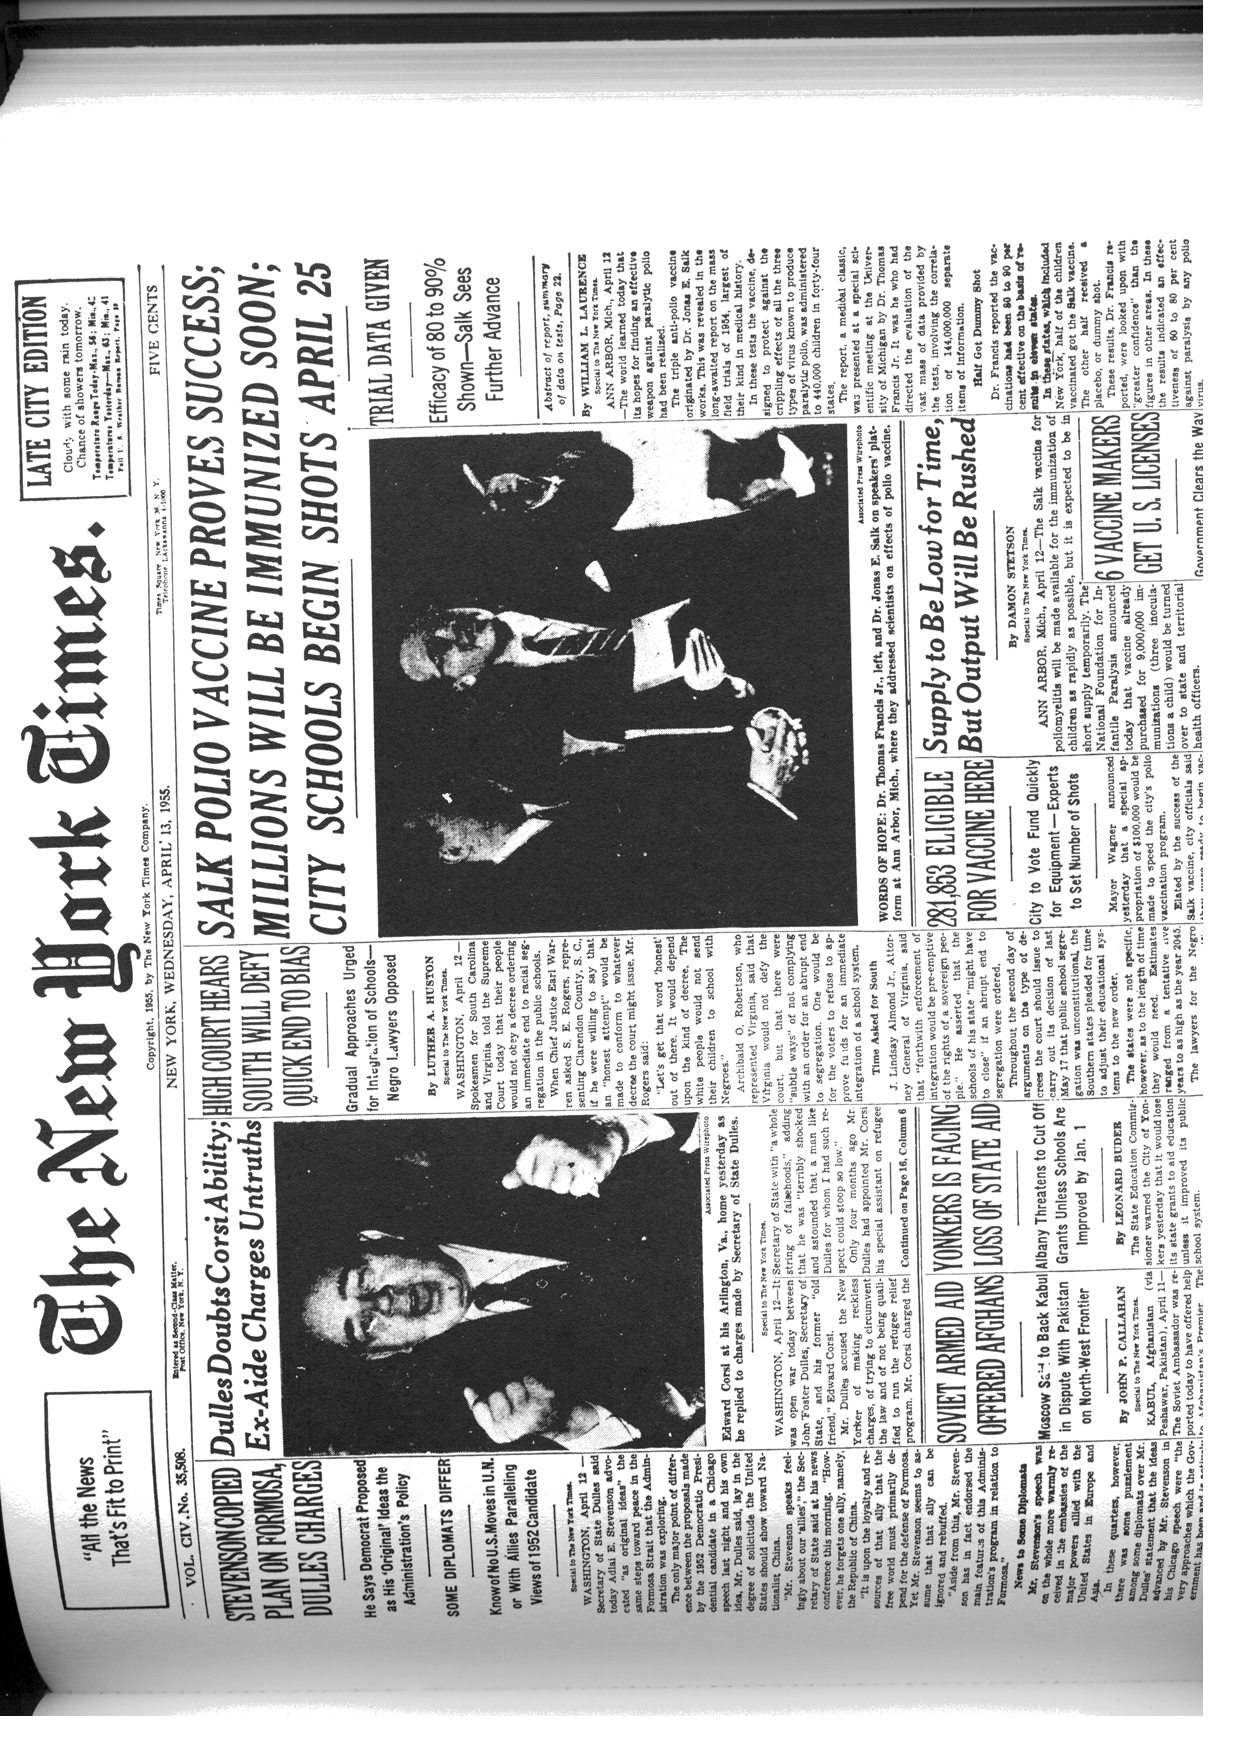
\includegraphics[width=15.00000cm]{salk_nytimes.pdf}
\caption{\label{fig:f-nytimes} Public reaction to statistical inference.}
\end{figure}

\chapter{Continuous variables: Population and sampling
distributions}\label{c-contd}

\section{Introduction}\label{s-contd-intro}

This chapter serves both as an explanation of some topics that were
skimmed over previously, and as preparation for later chapters. Its
central theme is probability distributions of continuous variables.
These may appear in two distinct roles:

\begin{itemize}
\item
  As population distributions of continuous variables, for instance
  blood pressure in the illustrative example of this chapter. This
  contrasts with the kinds of discrete variables that were considered in
  Chapters \ref{c-tables} and \ref{c-probs}. Methods of inference for
  continuous variables will be introduced in Chapters \ref{c-means} and
  \ref{c-regression}.
\item
  As sampling distributions of sample statistics. These are typically
  continuous even in analyses of discrete variables, such as in Chapter
  \ref{c-probs} where the variable of interest \(Y\) was binary but the
  sampling distributions of a sample proportion \(\hat{\pi}\) and the
  \(z\)-test statistic for population probability \(\pi\) were
  nevertheless continuous. We have already encountered two continuous
  distributions in this role, the \(\chi^{2}\) distributions in Chapter
  \ref{c-tables} and the standard normal distribution in Chapter
  \ref{c-probs}. Their origins are explained in more detail below.
\end{itemize}

To illustrate the concepts, we use data from the Health Survey for
England 2002 (HES).\footnote{ESS Round 5: European Social Survey Round 5
  Data (2010). Data file edition 2.0. Norwegian Social Science Data
  Services, Norway � Data Archive and distributor of ESS data. The full
  data can be obtained from \texttt{http://ess.nsd.uib.no/ess/round5/}.}
One part of the survey was a short physical examination by a nurse.
Figure \ref{fig:f-bp1} shows a histogram and frequency polygon of
diastolic blood pressure (in mm Hg) for 4489 respondents, measured by
the mean of the last two of three measurements taken during the
examination. Data from respondents for whom the measurements were not
obtained or were considered invalid have been excluded. Respondents aged
under 25 have also been excluded for simplicity, because this age group
was oversampled in the 2002 HES.

\begin{figure}[htbp]
\centering
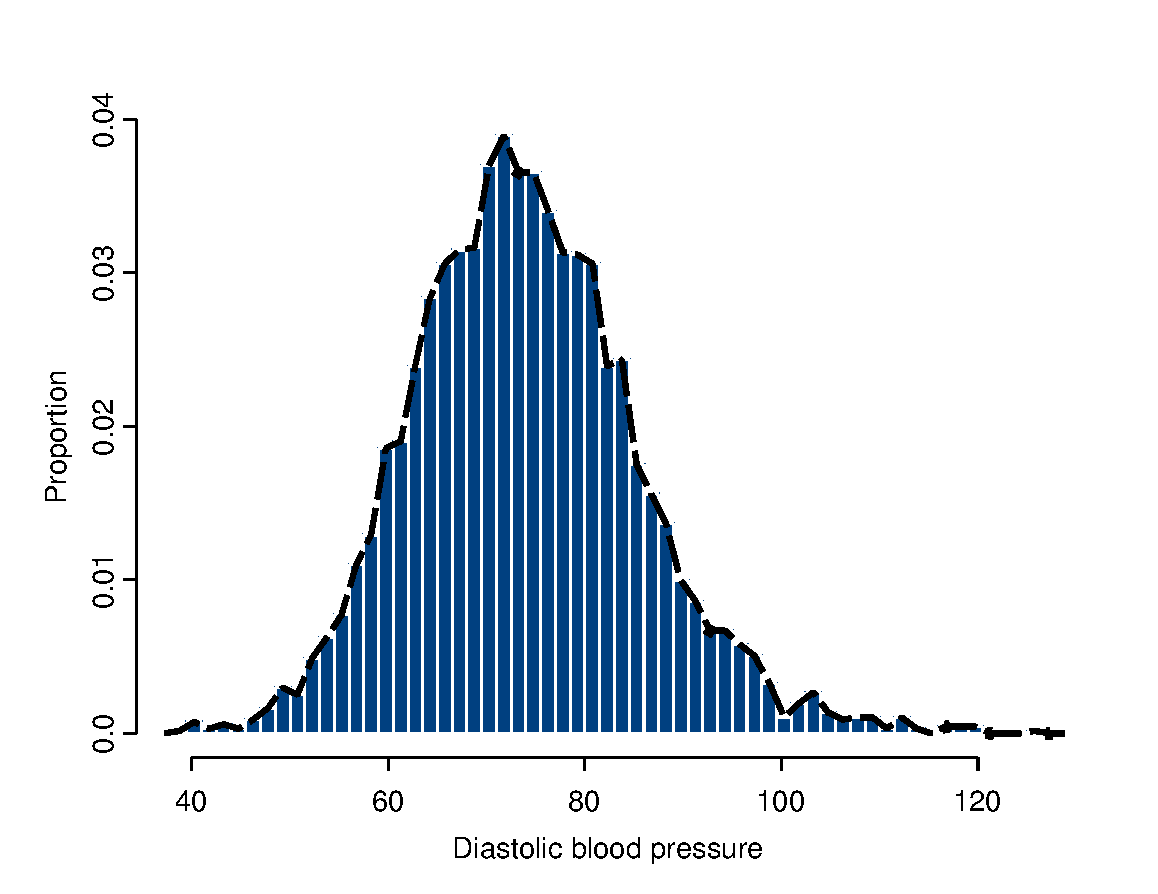
\includegraphics[width=13.50000cm]{bloodp1.pdf}
\caption{\label{fig:f-bp1} Histogram of diastolic blood pressure, with the
corresponding frequency polygon, from Health Survey for England 2002
(respondents aged 25 or over, \(n=4489\)).}
\end{figure}

The respondents whose blood pressures are summarized in Figure
\ref{fig:f-bp1} are in reality a sample from a larger population in the
sense of Sections \ref{s-samples-finpops} and \ref{s-samples-samples}.
However, for illustrative purposes we will here pretend that they are
actually an entire finite population of 4489 people (the adults in a
small town, say). The values summarised in Figure \ref{fig:f-bp1} then
form the population distribution of blood pressure in this population.
It is clear that blood pressure is best treated as a continuous
variable.

\section{Population distributions of continuous
variables}\label{s-contd-popdistrs}

\subsection{Population parameters and their point
estimates}\label{ss-contd-popdistrs-params}

If we knew all of its values, we could summarise a finite population
distribution by, say, a histogram like Figure \ref{fig:f-bp1}. We can
also consider specific characteristics of the distribution, i.e.~its
\emph{parameters} in the sense introduced in Section
\ref{s-probs-distribution}. For the distribution of a continuous
variable, the most important parameters are the \textbf{population mean}

\begin{equation}\mu=\frac{\sum Y_{i}}{N}
\label{eq:mu}\end{equation}

and the \textbf{population variance}

\begin{equation}\sigma^{2} = \frac{\sum (Y_{i}-\mu)^{2}}{N}
\label{eq:sigma2}\end{equation}

or, instead of the variance, the \textbf{population standard deviation}

\begin{equation}\sigma = \sqrt{\frac{\sum (Y_{i}-\mu)^{2}}{N}}.
\label{eq:sigma}\end{equation}

Here \(\mu\) and \(\sigma\) are the lower-case Greek letters ``mu'' and
``sigma'' respectively, and \(\sigma^{2}\) is read ``sigma squared''. It
is common to use Greek letters for population parameters, as we did also
for the probability parameter \(\pi\) in Chapter \ref{c-probs}.

In (\ref{eq:mu})--(\ref{eq:sigma}), \(N\) is the number of units in a
finite population and the sums indicated by \(\Sigma\) are over all of
these \(N\) units. If we treat the data in Figure \ref{fig:f-bp1} as a
population, \(N=4489\) and these population parameters are \(\mu=74.2\),
\(\sigma^{2}=127.87\) and \(\sigma=11.3\).

Because the formulas (\ref{eq:mu})--(\ref{eq:sigma}) involve the
population size \(N\), they apply in this exact form only to finite
populations like the one in this example (and as discussed more
generally in Section \ref{s-samples-finpops}) but not to infinite ones
of the kind discussed in Section \ref{s-samples-infpops}. However, the
definitions of \(\mu\), \(\sigma^{2}\), \(\sigma\) and other parameters
can be extended to apply also to infinite populations. These
definitions, which will be omitted here, involve the concept of
continuous probability distributions that is discussed in the next
section. The interpretations of the population parameters turn out to be
intuitively similar for both the finite and infinite-population cases,
and the same methods of analysis apply to both, so we can here ignore
the distinction without further comment.

The population formulas (\ref{eq:mu})--(\ref{eq:sigma}) clearly resemble
those of some sample statistics introduced in Chapter \ref{c-descr1},
specifically the \emph{sample} mean, variance and standard deviation

\begin{equation}\bar{Y}=\frac{\sum Y_{i}}{n}, \label{eq:Ybar-ch6}\end{equation}

\begin{equation}s^{2} = \frac{\sum (Y_{i}-\bar{Y})^{2}}{n-1}\label{eq:s2-ch6}\end{equation}

and

\begin{equation}s = \sqrt{\frac{\sum (Y_{i}-\bar{Y})^{2}}{n-1}}\label{eq:s-ch6}\end{equation}

where the sums are now over the \(n\) observations in a sample. These
can be used as descriptions of the sample distribution as discussed in
Chapter \ref{c-descr1}, but also as \emph{point estimates} of the
corresponding population parameters in the sense defined in Section
\ref{s-probs-pointest}. We may thus use the sample mean \(\bar{Y}\) as a
point estimate of the population mean \(\mu\), and the sample variance
\(s^{2}\) and sample standard deviation \(s\) as point estimates of
population variance \(\sigma^{2}\) and standard deviation \(\sigma\)
respectively. These same estimates can be used for both finite and
infinite population distributions.

For further illustration of the connection between population and sample
quantities, we have also drawn a simple random sample of \(n=50\)
observations from the finite population of \(N=4489\) observations in
Figure \ref{fig:f-bp1}. Table \ref{tab:t-bp-example} shows the summary
statistics (\ref{eq:Ybar-ch6}--(\ref{eq:s-ch6}) in this sample and the
corresponding parameters (\ref{eq:mu})--(\ref{eq:sigma}) in the
population.

\begin{longtable}[]{@{}lllrl@{}}
\caption{\label{tab:t-bp-example} Summary statistics for diastolic blood
pressure in the population and a sample from it in the example used for
illustration in Sections
\ref{s-contd-popdistrs}--\ref{s-contd-clt}.}\tabularnewline
\toprule
\begin{minipage}[t]{0.14\columnwidth}\raggedright\strut
\strut
\end{minipage} & \begin{minipage}[t]{0.12\columnwidth}\raggedright\strut
Size\strut
\end{minipage} & \begin{minipage}[t]{0.18\columnwidth}\raggedright\strut
Mean\strut
\end{minipage} & \begin{minipage}[t]{0.17\columnwidth}\raggedleft\strut
Standard Deviation\strut
\end{minipage} & \begin{minipage}[t]{0.23\columnwidth}\raggedright\strut
Variance\strut
\end{minipage}\tabularnewline
\begin{minipage}[t]{0.14\columnwidth}\raggedright\strut
Population\strut
\end{minipage} & \begin{minipage}[t]{0.12\columnwidth}\raggedright\strut
\(N=4489\)\strut
\end{minipage} & \begin{minipage}[t]{0.18\columnwidth}\raggedright\strut
\(\mu=74.2\)\strut
\end{minipage} & \begin{minipage}[t]{0.17\columnwidth}\raggedleft\strut
\(\sigma=11.3\)\strut
\end{minipage} & \begin{minipage}[t]{0.23\columnwidth}\raggedright\strut
\(\sigma^{2}=127.87\)\strut
\end{minipage}\tabularnewline
\begin{minipage}[t]{0.14\columnwidth}\raggedright\strut
Sample\strut
\end{minipage} & \begin{minipage}[t]{0.12\columnwidth}\raggedright\strut
\(n=50\)\strut
\end{minipage} & \begin{minipage}[t]{0.18\columnwidth}\raggedright\strut
\(\bar{Y}=72.6\)\strut
\end{minipage} & \begin{minipage}[t]{0.17\columnwidth}\raggedleft\strut
\(s=12.7\)\strut
\end{minipage} & \begin{minipage}[t]{0.23\columnwidth}\raggedright\strut
\(s^{2}=161.19\)\strut
\end{minipage}\tabularnewline
\bottomrule
\end{longtable}

You may have noticed that the formulas of the sample variance
(\ref{eq:s2-ch6}) and sample standard deviation (\ref{eq:s-ch6}) involve
the divisor \(n-1\) rather than the \(n\) which might seem more natural,
while the population formulas (\ref{eq:sigma2}) and (\ref{eq:sigma}) do
use \(N\) rather than \(N-1\). The reason for this is that using \(n-1\)
gives the estimators certain mathematically desirable properties
(\(s^{2}\) is an \emph{unbiased} estimate of \(\sigma^{2}\), but
\(\hat{\sigma}^{2}\) below is not). This detail need not concern us
here. In fact, the statistics which use \(n\) instead, i.e.

\begin{equation}\hat{\sigma}^{2}=\frac{\sum (Y_{i}-\bar{Y})^{2}}{n}
\label{eq:s2b}\end{equation}

for \(\sigma^{2}\) and \(\hat{\sigma}=\sqrt{\hat{\sigma}^{2}}\) for
\(\sigma\), are also sensible estimates and very similar to \(s^{2}\)
and \(s\) unless \(n\) is very small. In general, there are often
several possible sample statistics which could be used as estimates for
the same population parameter.

\section{Probability distributions of continuous
variables}\label{s-contd-probdistrs}

\subsection{General comments}\label{ss-contd-probdistrs-general}

Thinking about population distributions of continuous distributions
using, say, histograms as in Figure \ref{fig:f-bp1} would present
difficulties for statistical inference, for at least two reasons. First,
samples cannot in practice give us enough information to make reliable
inferences on all the details of a population distribution, such as the
small kinks and bumps of Figure \ref{fig:f-bp1}. Such details would
typically not even be particularly interesting compared to major
features like the central tendency and variation of the population
distribution. Second, this way of thinking about the population
distribution is not appropriate when the population is regarded as
infinite.

Addressing both of these problems requires one more conceptual leap.
This is to make the assumption that the population distribution is
well-represented by a continuous \emph{probability distribution}, and
focus on inference on the parameters of that distribution.

We have already introduced the concept of probability distributions in
Section \ref{s-samples-popdistrs}, and considered instances of it in
Chapters \ref{c-tables} and \ref{c-probs}. There, however, the term was
not emphasised because it added no crucial insight into the methods of
inference. This was because for discrete variables a probability
distribution is specified simply by listing the probabilities of all the
categories of the variable. The additional terminology of probability
distributions and their parameters seems almost redundant in that
context.

The situation is very different for continuous variables. This is
illustrated by Figure \ref{fig:f-bp2}, which shows the same frequency
polygon as in Figure \ref{fig:f-bp1}, now supplemented by a smooth
curve. This curve (``a probability density function'') describes a
particular probability distribution. It can be thought of as a smoothed
version of the shape of the frequency polygon. What we will do in the
future is to use some such probability distribution to represent the
population distribution. This means effectively arguing that we believe
that the shape of the true population distribution is sufficiently
regular to be well described by a smooth curve such as the one in Figure
\ref{fig:f-bp2}.

In Figure \ref{fig:f-bp2} the curve and the frequency polygon have
reasonably similar shapes, so the assumption that the former is a good
representation of the latter does not seem far-fetched. However, the two
are clearly not exactly the same, nor do we expect that even the blood
pressures of all English adults exactly match this curve or any other
simple probability distribution. All we require is that a population
distribution is close enough to a specified probability distribution for
the results from analyses based on this assumption to be meaningful and
not misleading.

\begin{figure}[htbp]
\centering
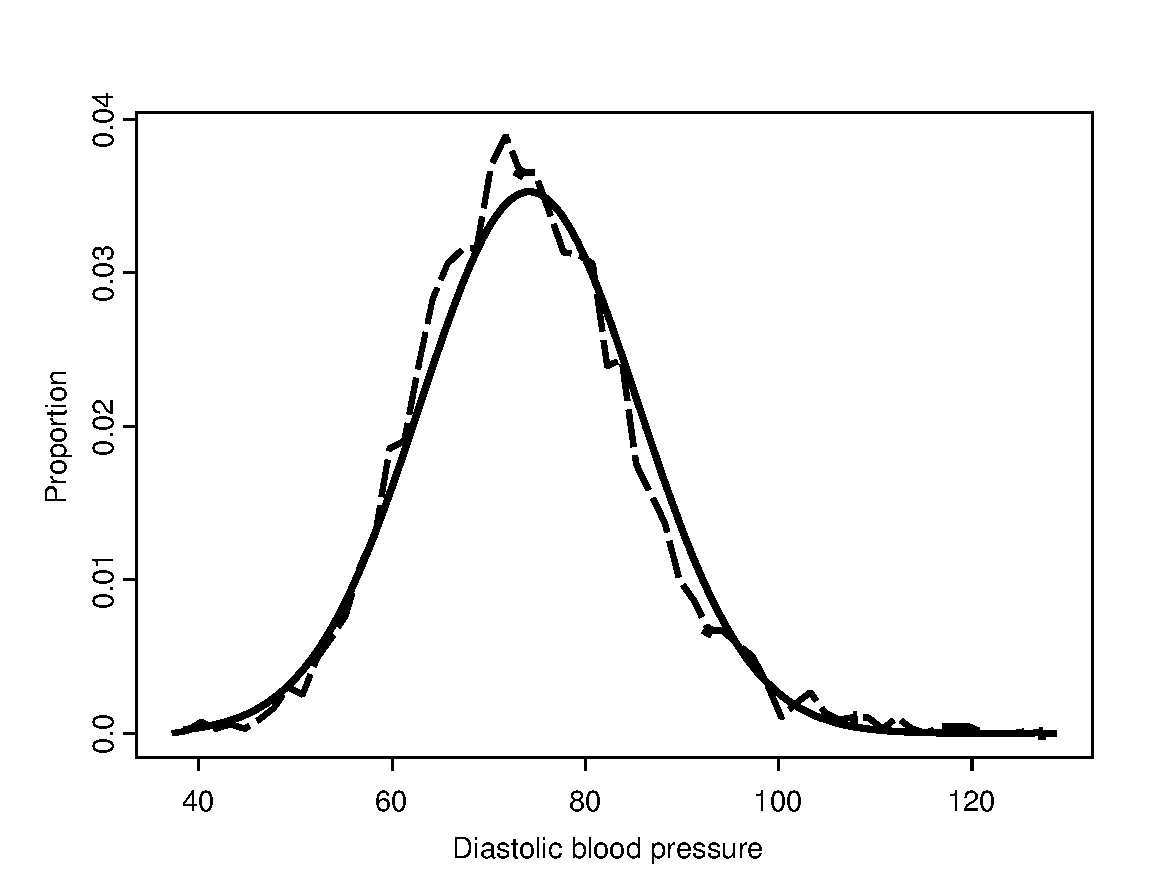
\includegraphics[width=11.50000cm]{bloodp2.pdf}
\caption{\label{fig:f-bp2} The frequency polygon of Figure \ref{fig:f-bp1},
together with a normal curve with the same mean and variance.}
\end{figure}

\label{p-model} Such a simplifying assumption about the population
distribution is known as a \textbf{statistical model} for the
population. The reason for working with a model is that it leads to much
simpler methods of analysis than would otherwise be required. For
example, the shape of the distribution shown in Figure \ref{fig:f-bp2}
is entirely determined by just two parameters, its mean and variance.
Under this model, all questions about the population distribution can
thus be reduced to questions about these two population parameters, and
inference can focus on tests and confidence intervals for them.

The potential cost of choosing a specific probability distribution as
the statistical model for a particular application is that the
assumption may be inappropriate for the data at hand, and if it is,
conclusions about population parameters derived from analyses based on
this assumption may be misleading. The distribution should thus be
chosen carefully, usually based on both substantive considerations and
initial descriptive examination of the observed data.

For example, the particular probability distribution shown in Figure
\ref{fig:f-bp2}, which is known as the normal distribution, is by
definition symmetric around its mean. While it is an adequate
approximation of many approximately symmetric population distributions
of continuous variables, such as that of blood pressure, many other
population distributions are not even roughly symmetric. It would be
unrealistic to assume the population distributions of such variables to
be normal. Instead, we might consider other continuous probability
distributions which can be skewed. Examples of these are the
\emph{Exponential}, \emph{Gamma}, \emph{Weibull}, and \emph{Beta}
distributions. \emph{Discrete} distributions, of course, will require
quite different probability disributions, such as the \emph{Binomial}
distribution discussed in Chapter \ref{c-probs}, or the
\emph{Multinomial} and \emph{Poisson} distributions. On this course,
however, we will not include further discussion of these various
possibilities.

\subsection{The normal distribution as a population
distribution}\label{ss-contd-probdistrs-normal}

The particular probability distribution that is included in Figure
\ref{fig:f-bp2} is a \textbf{normal distribution}, also known as the
\emph{Gaussian} distribution, after the great German mathematician Karl
Friedrich Gauss who was one of the first to derive it in 1809. Figure
\ref{fig:f-10dm} shows a portrait of Gauss from the former German 10-DM
banknote, together with pictures of the university town of Göttingen and
of the normal curve (even the mathematical formula of the curve is
engraved on the note). The curve of the normal distribution is also
known as the ``bell curve'' because of its shape.

\begin{figure}[htbp]
\centering
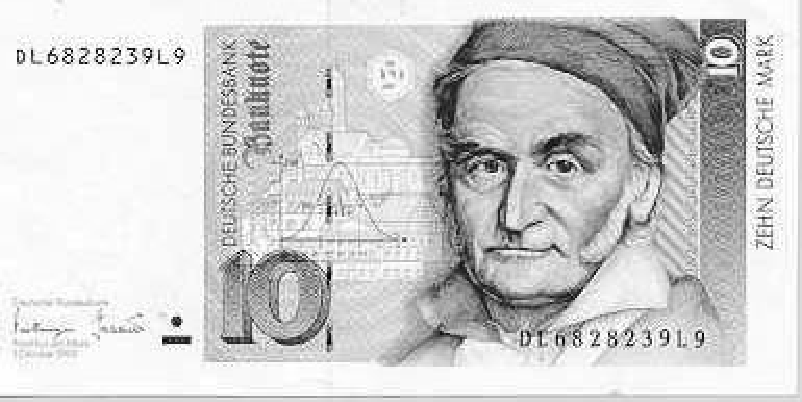
\includegraphics[width=14.00000cm]{mark.pdf}
\caption{\label{fig:f-10dm} A portrait of Gauss and the normal curve on a
former German 10-DM banknote.}
\end{figure}

The normal distribution is by far the most important probability
distribution in statistics. The main reason for this is its use as a
sampling distribution in a wide range of contexts, for reasons that are
explained in Section \ref{s-contd-clt}. However, the normal distribution
is also useful for describing many approximately symmetric population
distributions, and it is in this context that we introduce its
properties first.

A normal distribution is completely specified by two numbers, its mean
(or ``expected value'') \(\mu\) and variance \(\sigma^{2}\). This is
sometimes expressed in notation as \(Y\sim N(\mu, \sigma^{2})\), which
is read as ``\(Y\) is normally distributed with mean \(\mu\) and
variance \(\sigma^{2}\)''. Different values for \(\mu\) and
\(\sigma^{2}\) give different distributions. For example, the curve in
Figure \ref{fig:f-bp2} is that of the \(N(74.2, \, 127.87)\)
distribution, where the mean \(\mu=74.2\) and variance
\(\sigma^{2}=127.87\) are the same as the mean and variance calculated
from formulas (\ref{eq:mu}) and (\ref{eq:sigma2}) for the 4489
observations of blood pressure. This ensures that this particular normal
curve best matches the frequency polygon in Figure \ref{fig:f-bp2}.

The mean \(\mu\) describes the central tendency of the distribution, and
the variance \(\sigma^{2}\) its variability. This is illustrated by
Figure \ref{fig:f-3norms}, which shows the curves for three different
normal distributions. The mean of a normal distribution is also equal to
both its median and its mode. Thus \(\mu\) is the central value in the
sense that it divides the distribution into two equal halves, and it
also indicates the peak of the curve (the highest probability, as
discussed below). In Figure \ref{fig:f-3norms}, the curves for
\(N(0, 1)\) and \(N(0, 9)\) are both centered around \(\mu=0\); the mean
of the \(N(5, 1)\) distribution is \(\mu=5\), so the whole curve is
shifted to the right and centered around 5.

\begin{figure}[htbp]
\centering
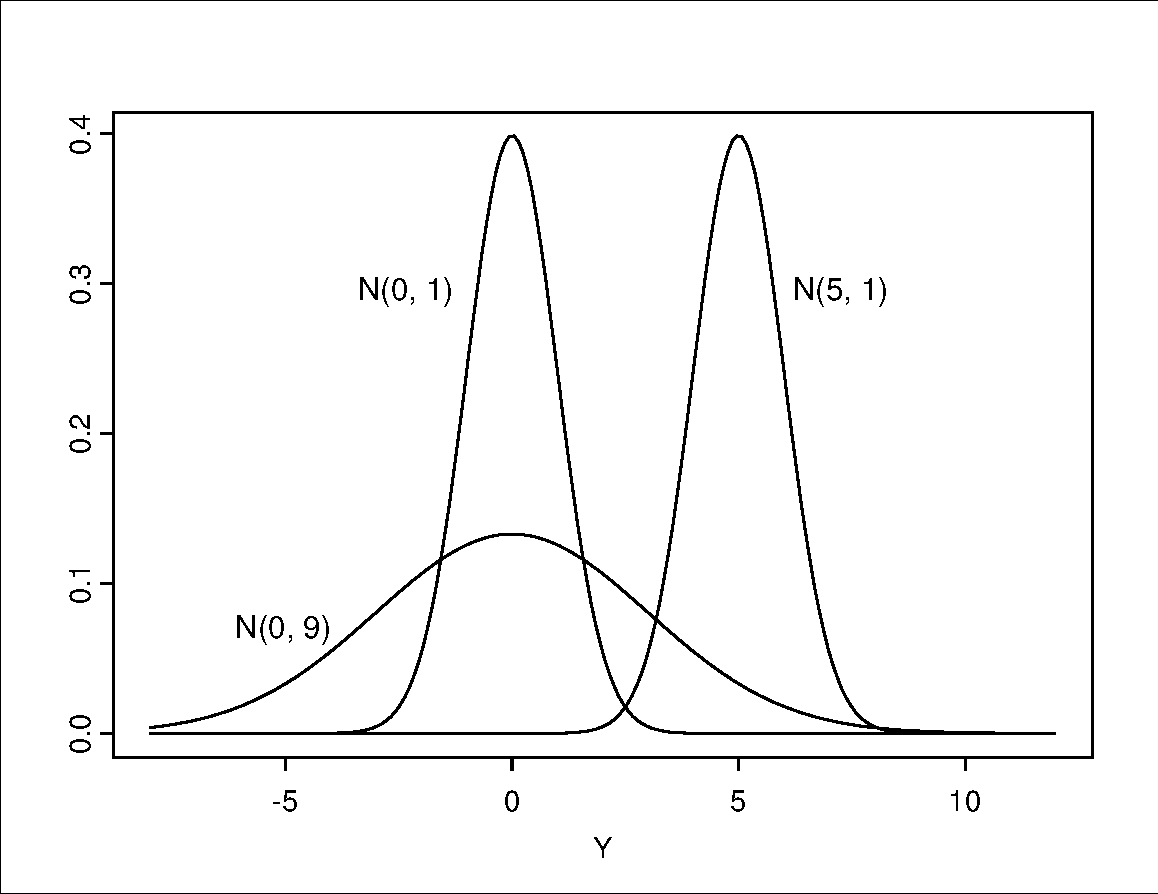
\includegraphics[width=11.00000cm]{threenorms.pdf}
\caption{\label{fig:f-3norms} Three normal distributions with different
means and/or variances.}
\end{figure}

The variance \(\sigma^{2}\) determines how widely spread the curve is.
In Figure \ref{fig:f-3norms}, the curves for \(N(0, 1)\) and \(N(5, 1)\)
have the same variance \(\sigma^{2}=1\), so they have the same shape in
terms of their spread. The curve for \(N(0, 9)\), on the other hand, is
more spread out, because it has a higher variance of \(\sigma^{2}=9\).
As before, it is often more convenient to describe variability in terms
of the standard deviation \(\sigma\), which is the square root of the
variance. Thus we may also say that the \(N(0, 9)\) distribution has the
standard deviation \(\sigma=\sqrt{9}=3\) (for \(\sigma^{2}=1\) the two
numbers are the same, since \(\sqrt{1}=1\)).

In the histogram in Figure \ref{fig:f-bp1}, the heights of the bars
correspond to the proportions of different ranges of blood pressure
among the 4489 people in the data set. Another way of stating this is
that if we were to sample a person from this group at random, the
heights of the bars indicate the \textbf{probabilities} that the
selected person's blood pressure would be in a particular range. Some
values are clearly more likely than others. For example, for blood
pressures in the range 50--51.5, the probability is about 0.0025,
corresponding to a low bar, while for the range 74--75.5 it is about
0.0365, corresponding to a much higher bar.

The interpretation is the same for the curve of a continuous probability
distribution. Its height also indicates the probability of different
values in random sampling from a population with that distribution. More
precisely, the \emph{areas} under the curve give such probabilities for
ranges of values. Probabilities of all the possible values must add up
to one, so the area under the whole curve is one --- i.e.~a randomly
sampled unit must have \emph{some} value of the variable in question.
More generally, the area under the curve for a range of values gives the
probability that the value of a randomly sampled observation is in that
range. These are the same principles that we have already used to derive
\(P\)-values for tests in Sections \ref{ss-tables-chi2test-Pval} and
\ref{ss-probs-test1sample-samplingd}.

\begin{figure}[htbp]
\centering
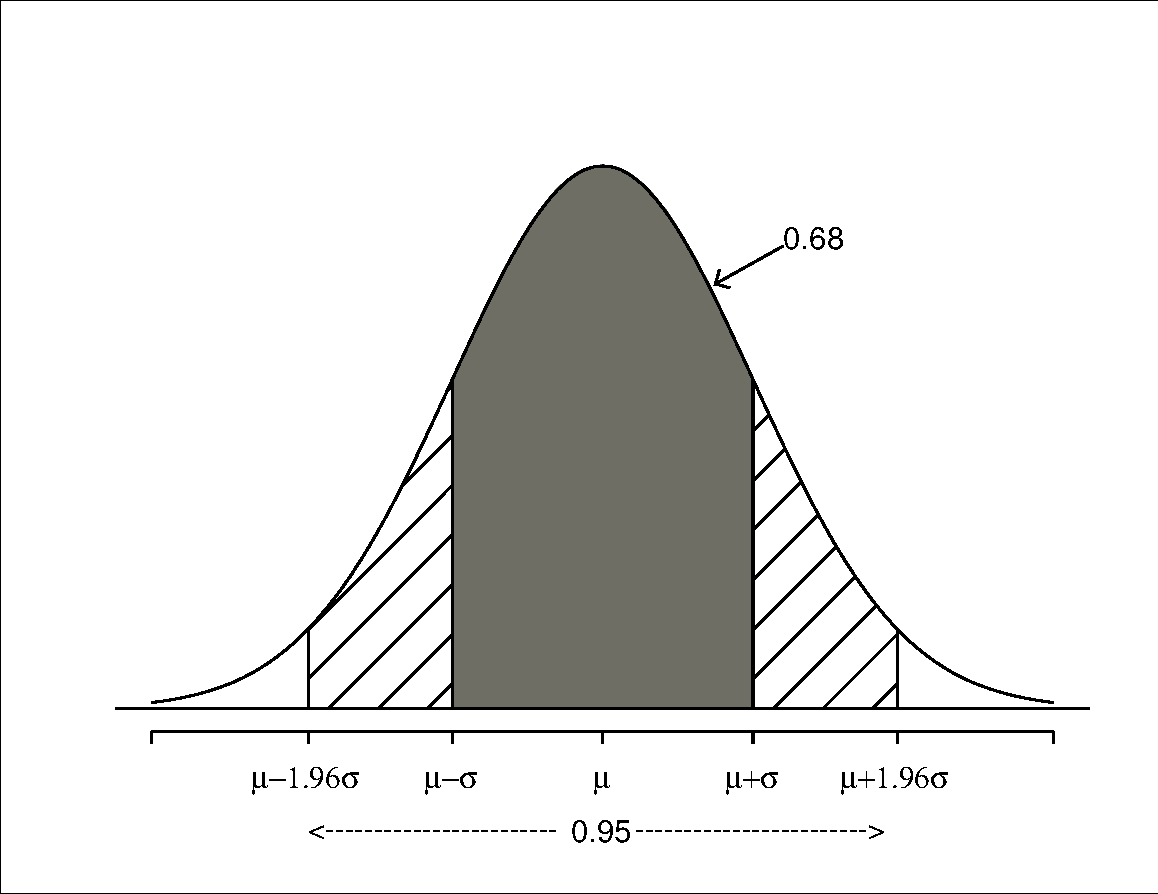
\includegraphics[width=12.00000cm]{norm1.pdf}
\caption{\label{fig:f-norm1} Illustration of probabilities for the normal
distribution. The probability of an observation being within one
standard deviation of the mean (the grey area) is 0.68, and the
probability of it being within 1.96 standard deviations of the mean
(grey and shaded areas together) is 0.95.}
\end{figure}

Figure \ref{fig:f-norm1} illustrates this further with some results
which hold for any normal distribution, whatever its mean and variance.
The grey area in the figure corresponds to values from \(\mu-\sigma\) to
\(\mu+\sigma\), i.e.~those values which are no further than one standard
deviation from the mean. The area of the grey region is 0.68, so the
probability that a randomly sampled value from a normal distribution is
within one standard deviation of the mean is 0.68. The two shaded
regions either side of the grey area extend the area to 1.96 standard
deviations below and above the mean. The probability of this region (the
grey and shaded areas together) is 0.95. Rounding the 1.96 to 2, we can
thus say that approximately 95\% of observations drawn from a normal
distribution tend to be within two standard deviations of the mean. This
leaves the remaining 5\% in the two tails of the distribution, further
than 1.96 standard deviations from the mean (the two white areas in
Figure \ref{fig:f-norm1}). Because the normal distribution is symmetric,
these two areas are of equal size and each thus has the probability
0.025 (i.e.~0.05/2).

Such calculations can also be used to determine probabilities in
particular examples. Returning to the blood pressure data, we might for
example be interested in

\begin{itemize}
\item
  the proportion of people in some population whose diastolic blood
  pressure is higher than 90 (one possible cut-off point for high blood
  pressure or hypertension)
\item
  the proportion of people with diastolic blood pressure below 60
  (possibly indicating unusually low blood pressure or hypotension)
\item
  the proportion of people in the normal pressure range of 60--90
\end{itemize}

Such figures might be of interest for example for predicting health
service needs for treating hypertension. Suppose that we were reasonably
confident (perhaps from surveys like the one described above) that the
distribution of diastolic blood pressure in the population of interest
was approximately normally distributed with mean 74.2 and variance
127.87 (and thus standard deviation 11.3). The probabilities of interest
are then the areas of the regions shown in Figure \ref{fig:f-normbp}.

The remaining question is how to calculate such probabilities. The short
answer is ``with a computer''. However, to explain an approach which is
required for this in some computer packages and also to provide an
alternative method which does not require a computer, we need to
introduce one more new quantity. This is the \textbf{Z score}, which is
defined as

\begin{equation}Z = \frac{Y-\mu}{\sigma}
\label{eq:Zscore}\end{equation}

where \(Y\) can be any value of the variable of interest. For example,
in the blood pressure example the \(Z\) scores corresponding to values
60 and 90 are \(Z=(60-74.2)/11.3=-1.26\) and \(Z=(90-74.2)/11.3=1.40\)
respectively. The \(Z\) score can be interpreted as the distance of the
value \(Y\) from the mean \(\mu\), measured in standard deviations
\(\sigma\). Thus the blood pressure 60, with a \(Z\) score of \(-1.26\),
is 1.26 standard deviations \emph{below} (hence the negative sign) the
mean, while 90 (with \(Z\) score 1.40) is 1.40 standard deviations
\emph{above} the mean.

\begin{figure}[htbp]
\centering
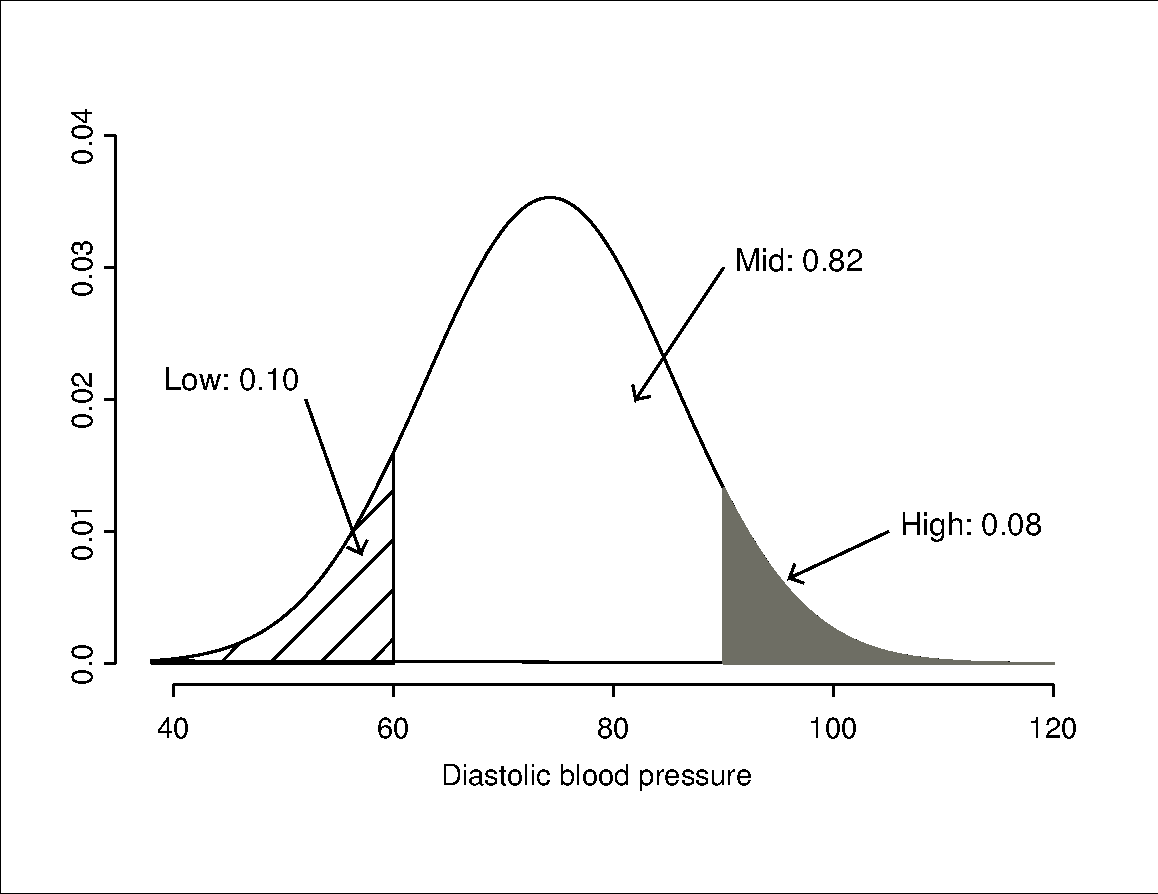
\includegraphics[width=12.00000cm]{normbp.pdf}
\caption{\label{fig:f-normbp} Illustration of probabilities for a normal
distribution in the blood pressure example, where \(\mu=74.2\) and
\(\sigma=11.3\). The plot shows probabilities for the ranges of values
at most 60 (``Low''), between 60 and 90 (``Mid'') and over 90
(``High'').}
\end{figure}

\begin{longtable}[]{@{}rr@{}}
\caption{\label{tab:t-normtab} Extract from the table of right-hand tail
probabilities for normal \(Z\) scores. Here ``Tail Prob.'' is the
probability that a value from the standard normal distribution is at
least the value in the column labelled ``\(z\)''. The full table is
shown in Section \ref{s-disttables-Z}.}\tabularnewline
\toprule
\(z\) & Tail Prob.~\tabularnewline
\midrule
\endfirsthead
\toprule
\(z\) & Tail Prob.~\tabularnewline
\midrule
\endhead
\(\vdots\) & \(\vdots\)\tabularnewline
1.24 & 0.1075\tabularnewline
1.25 & 0.1056\tabularnewline
1.26 & 0.1038\tabularnewline
1.27 & 0.1020\tabularnewline
\(\vdots\) & \(\vdots\)\tabularnewline
1.38 & 0.0838\tabularnewline
1.39 & 0.0823\tabularnewline
1.40 & 0.0808\tabularnewline
1.41 & 0.0793\tabularnewline
\(\vdots\) & \(\vdots\)\tabularnewline
\bottomrule
\end{longtable}

The probability distribution of the \(Z\) scores is a normal
distribution with mean 0 and variance 1, i.e.~\(Z\sim N(0,1)\). This is
known as the \textbf{standard normal distribution}. The usefulness of
\(Z\) scores lies in the fact that by transforming the original variable
\(Y\) from the \(N(\mu, \sigma^{2}\)) distribution into the standard
normal distribution they remove the specific values of \(\mu\) and
\(\sigma\) from the calculation. With this trick, probabilities for any
normal distribution can be calculated using a single table for \(Z\)
scores. Such a table is given in Section \ref{s-disttables-Z} in the
Appendix, and an extract from it is shown in Table \ref{tab:t-normtab}
(note that it is not always presented exactly like this, as different
books may use slightly different format or notation). The first column
lists values of the \(Z\) score (a full table would typically give all
values from 0.00 to about 3.50). The second column, labelled ``Tail
Prob.'', gives the probability that a \(Z\) score for a normal
distribution is \emph{larger than} the value given by \(z\), i.e.~the
area of the region to the right of \(z\).

Consider first the probability that blood pressure is greater than 90,
i.e.~the area labelled ``High'' in Figure \ref{fig:f-normbp}. We have
seen that 90 corresponds to a \(Z\) score of 1.40, so the probability of
high blood pressure is the same as the probability that the normal \(Z\)
score is greater than 1.40. The row for \(z=1.40\) in the table tells us
that this probability is 0.0808, or 0.08 when rounded to two decimal
places as in Figure \ref{fig:f-normbp}.

The second quantity of interest was the probability of a blood pressure
at most 60, i.e.~the area of the ``Low'' region in Figure
\ref{fig:f-normbp}. The corresponding \(Z\) score is \(-1.26\). The
table, however, shows only positive values of \(z\). This is because we
can use the symmetry of the normal distribution to reduce all such
questions to ones about positive values of \(z\). Because the
distribution is symmetric, the probability that a \(Z\) score is
\emph{at most} \(-1.26\) (the area of the left-hand tail to the left of
\(-1.26\)) is the same as the probability that it is \emph{at least}
1.26 (the area of the right-hand tail to the right of 1.26). This is the
kind of quantity we calculated above\footnote{The data were obtained
  from
  \url{http://data.london.gov.uk/datastore/package/london-borough-profiles}.

  \noindentIf you download the ``Profiles in Excel'' workbook, you will
  find that one of the pages contains a map of the boroughs, and a tool
  for visualising the data on that map. A regular map of the boroughs
  can be found at for example at

  \url{http://www.londoncouncils.gov.uk/londonfacts/londonlocalgovernment/londonmapandlinks/default.htm}.}.
The required probability is thus equal to the right-hand tail
probability for 1.26, which the table shows to be 0.1038 (rounded to
0.10 in Figure \ref{fig:f-normbp}).

Finally, the probability of the ``Mid'' range of blood pressure is the
remaining probability not in the two other regions. Because the whole
area under the curve (the total probability) is 1, the required
probability is obtained by subtraction as \(1-(0.0808+0.1038)=0.8154\).
In this example these values obtained from the normal approximation of
the population distribution are very accurate. The exact proportions of
the 4489 respondents who had diastolic blood pressure at most 60 or
greater than 90 were 0.0996 and 0.0793 respectively, so rounded to two
decimal places they were the same as the 0.10 and 0.08 obtained from the
normal approximation.

These days we can use statistical computer programs to calculate such
probabilities directly for a normal distribution with any mean and
standard deviation. For example, SPSS has a function called
\texttt{CDF.NORMAL(}\emph{quant,mean,stddev}\texttt{)} for this purpose.
It calculates the probability that the value from a normal distribution
with mean \emph{mean} and standard deviation \emph{stddev} is \textbf{at
most} \emph{quant}.

In practice we do not usually know the population mean and variance, so
their sample estimates will be used in such calculations. For example,
for the sample in Table \ref{tab:t-bp-example} we had \(\bar{Y}=72.6\)
and \(s=12.7\). Using these values in a similar calculation as above
gives the estimated proportion of people in the population with
diastolic blood pressures over 90 as 8.5\%. Even with a sample of only
50 observations, the estimate is reasonably close to the true population
proportion of about 8.1\%.

\section{The normal distribution as a sampling
distribution}\label{s-contd-clt}

We have already encountered the normal distribution in Section
\ref{ss-probs-test1sample-samplingd}, in the role of the \emph{sampling
distribution} of a test statistic rather than as a model for the
population distribution of a variable. In fact, the most important use
of the normal distribution is as a sampling distribution, because in
this role it often cannot be replaced by any other simple distributions.
The reasons for this claim are explained in this section. We begin with
the case of the distribution of the sample mean in samples from a normal
population, before extending it with a result which provides the
justification for the standard normal sampling distributions used for
inference on proportions in Chapter \ref{c-probs}, and even for the
\(\chi^{2}\) sampling distribution of the \(\chi^{2}\) test in Chapter
\ref{c-tables}.

Recall from Section \ref{ss-tables-chi2test-sdist} that the sampling
distribution of a statistic is its distribution across all possible
random samples of a given size from a population. The statistic we focus
on here is the sample mean \(\bar{Y}\). If we assume that the population
distribution is exactly normal, we have the following result:

\begin{itemize}
\tightlist
\item
  If the population distribution of a variable \(Y\) is normal with mean
  \(\mu\) and variance \(\sigma^{2}\), the sampling distribution of the
  sample mean \(\bar{Y}\) for a random sample of size \(n\) is also a
  normal distribution, with mean \(\mu\) and variance \(\sigma^{2}/n\).
\end{itemize}

The mean and variance of this sampling distribution are worth discussing
separately:

\begin{itemize}
\item
  The mean of the sampling distribution of \(\bar{Y}\) is equal to the
  population mean \(\mu\) of \(Y\). This means that while \(\bar{Y}\)
  from a single sample may be below or above the true \(\mu\), in
  repeated samples it would on average estimate the correct parameter.
  In statistical language, \(\bar{Y}\) is then an \emph{unbiased
  estimate} of \(\mu\). More generally, most possible samples would give
  values of \(\bar{Y}\) not very far from \(\mu\), where the scale for
  ``far'' is provided by the standard deviation discussed below.
\item
  The variance of the sampling distribution of \(\bar{Y}\) is
  \(\sigma^{2}/n\) or, equivalently, its standard deviation is
  \(\sigma/\sqrt{n}\). This standard deviation is also known as the
  \textbf{standard error of the mean}, and is often denoted by something
  like \(\sigma_{\bar{Y}}\). It describes the variability of the
  sampling distribution. Its magnitude depends on \(\sigma\), i.e.~on
  the variability of \(Y\) in the population. More interestingly, it
  also depends on the sample size \(n\), which appears in the
  denominator in \(\sigma/\sqrt{n}\). This means that the standard error
  of the mean is smaller for large samples than for small ones. This is
  illustrated in Figure \ref{fig:f-sampld2}. It shows the sampling
  distribution of \(\bar{Y}\) for samples of sizes \(n=50\) and
  \(n=1000\) from a normal population with \(\mu=74.2\) and
  \(\sigma=11.3\), i.e.~the population mean and standard deviation in
  the blood pressure example. It can be seen that while both sampling
  distributions are centered around the true mean \(\mu=74.2\), the
  distribution for the smaller sample is more spread out than that for
  the larger sample: more precisely, the standard error of the mean is
  \(\sigma/\sqrt{n}=11.3/\sqrt{50}=1.60\) when \(n=50\) and
  \(11.3/\sqrt{1000}=0.36\) when \(n=1000\). Recalling from Section
  \ref{ss-contd-probdistrs-normal} that approximately 95\% of the
  probability in a normal distribution is within two standard deviations
  of the mean, this means that about 95\% of samples of size 50 in this
  case would give a value of \(\bar{Y}\) between
  \(\mu-2*1.60=74.2-3.2=71.0\) and \(74.2+3.2=77.4\). For samples of
  size \(n=1000\), on the other hand, 95\% of samples would yield
  \(\bar{Y}\) in the much narrower range of \(74.2-2*0.36=73.5\) to
  \(74.2+2*0.36=74.9\).
\end{itemize}

\begin{figure}[htbp]
\centering
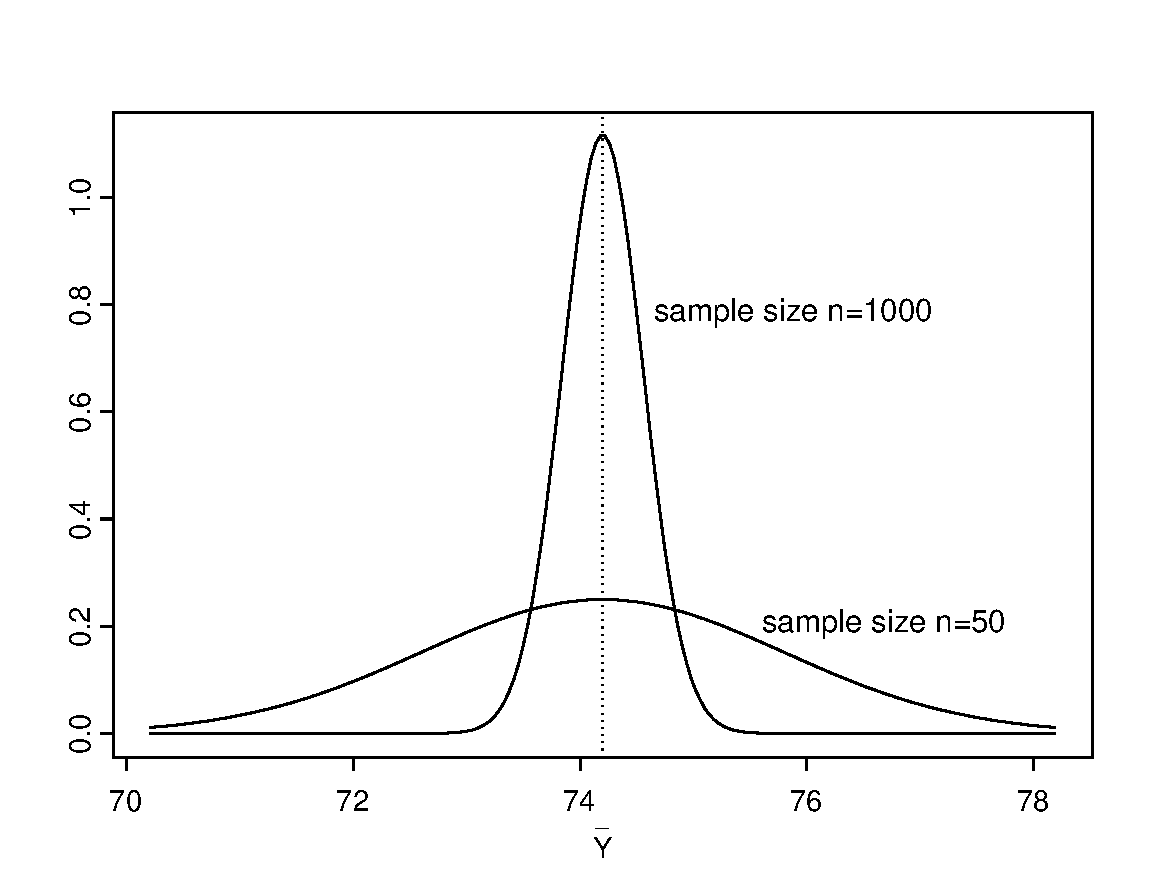
\includegraphics[width=12.00000cm]{sampld2_bp.pdf}
\caption{\label{fig:f-sampld2} Illustration of the sampling distribution of
the sample mean for two sample sizes. In both cases the population
distribution is normal with \(\mu=74.2\) and \(\sigma=11.3\).}
\end{figure}

The connection between sample size and the variability of a sampling
distribution applies not only to the sample mean but to (almost) all
estimates of population parameters. In general, (i) the task of
statistical inference is to use information in a sample to draw
conclusions about population parameters; (ii) the expected magnitude of
the sampling error, i.e.~the remaining uncertainty about population
parameters resulting from having information only on a sample, is
characterised by the variability of the sampling distributions of
estimates of the parameters; and (iii) other things being equal, the
variability of a sampling distribution decreases when the sample size
increases. Thus data really are the currency of statistics and more data
are better than less data. In practice data collection of course costs
time and money, so we cannot always obtain samples which are as large as
we might otherwise want. Apart from resource constraints, the choice of
sample size depends also on such things as the aims of the analysis, the
level of precision required, and guesses about the variability of
variables in the population. Statistical considerations of the
trade-offs between them in order to make decisions about sample sizes
are known as \emph{power} calculations. They will be discussed very
briefly later, in Section \ref{ss-means-tests3-power}.

In Figure \ref{fig:f-sampld} we use a computer simulation rather than a
mathematical theorem to examine the sampling distribution of a sample
mean. Here 100,000 simple random samples of size \(n=50\) were drawn
from the \(N=4489\) values of blood pressure that we are treating as the
finite population in this illustration. The sample mean \(\bar{Y}\) of
blood pressure was calculated for each of these samples, and the
histogram of these 100,000 values of \(\bar{Y}\) is shown in Figure
\ref{fig:f-sampld}. Also shown is the curve of the normal distribution
with the mean \(\mu\) and standard deviation \(\sigma/\sqrt{50}\)
determined by the theoretical result given above.

\begin{figure}[htbp]
\centering
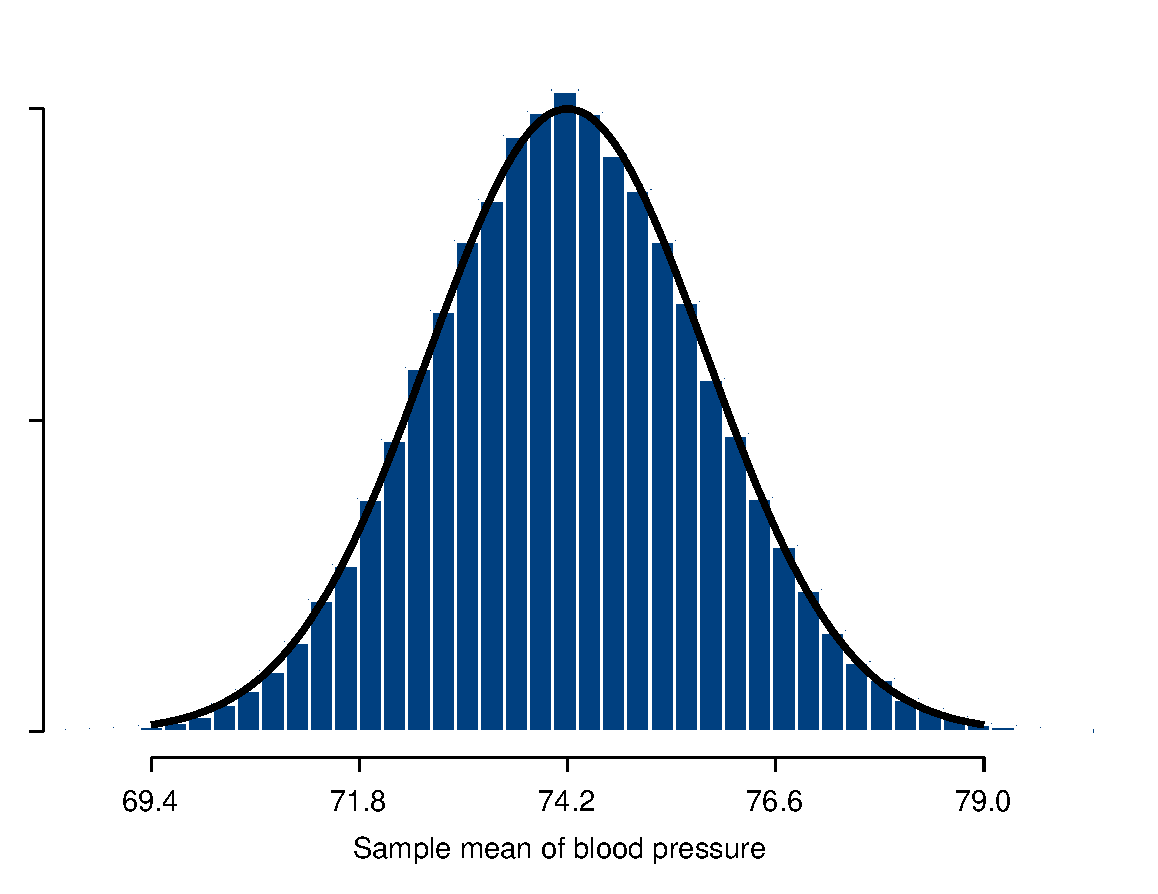
\includegraphics[width=12.00000cm]{sampld1_bp.pdf}
\caption{\label{fig:f-sampld} Example of the sampling distribution of the
sample mean. The plot shows a histogram of the values of the sample mean
in 100,000 samples of size \(n=50\) drawn from the 4489 values of
diastolic blood pressure shown in Figure \ref{fig:f-bp1}, for which the
mean is \(\mu=74.2\) and standard deviation is \(\sigma=11.3\).
Superimposed on the histogram is the curve of the approximate sampling
distribution, which is normal with mean \(\mu\) and standard deviation
\(\sigma/\sqrt{n}\).}
\end{figure}

The match between the curve and the histogram in Figure
\ref{fig:f-sampld} is clearly very close. This is actually a nontrivial
finding which illustrates a result which is of crucial importance for
statistical inference. Recall that the normal curve shown in Figure
\ref{fig:f-sampld} is derived from the mathematical result stated above,
which assumed that the population distribution of \(Y\) is
\emph{exactly} normal. The histogram in Figure \ref{fig:f-sampld}, on
the other hand, is based on repeated samples from the actual population
distribution of blood pressure, which, while quite close to a normal
distribution as shown in Figure \ref{fig:f-bp2}, is certainly not
exactly normal. Despite this, it is clear that the normal curve
describes the histogram essentially exactly.

If this was not true, that is if the sampling distribution that applies
for the normal distribution was inadequate when the the true population
distribution was even slightly different from normal, the result would
be of little practical use. No population distribution is ever exactly
normal, and many are very far from normality. Fortunately, however, it
turns out that quite the opposite is true, and that the sampling
distribution of the mean is approximately the same for nearly \emph{all}
population distributions. This is the conclusion from the
\textbf{Central Limit Theorem} (CLT), one of the most remarkable results
in all of mathematics. Establishing the CLT with increasing levels of
generality has been the work of many mathematicians over several
centuries, as different versions of it have been proved by, among
others, de Moivre, Laplace, Cauchy, Chebyshev, Markov, Liapounov,
Lindeberg, Feller, Lévy, Hoeffding, Robbins, and Rebolledo between about
1730 and 1980. One version of the CLT can be stated as

\textbf{The (Lindeberg-Feller) Central Limit Theorem}: For each
\(n=1,2,\dots\), let \(Y_{nj}\), for \(j=1,2,\dots,n\), be independent
random variables with \(\text{E}(Y_{nj})=0\) and
\(\text{var}(Y_{nj})=\sigma^{2}_{nj}\). Let
\(Z_{n}=\sum_{j=1}^{n} Y_{nj}\), and let
\(B^{2}_{n}=\text{var}(Z_{n})=\sum_{j=1}^{n} \sigma^{2}_{nj}\). Suppose
also that the following condition holds: for every \(\epsilon>0\),

\begin{equation}\frac{1}{B_{n}^{2}}\,
\sum_{j=1}^{n} \, \text{E}\{ Y_{nj}^{2} I(|Y_{nj}|\ge \epsilon B_{n})\}
\rightarrow 0 \; \text{  as  } \; n\rightarrow \infty.
\label{eq:lindeberg}\end{equation}

Then \(Z_{n}/B_{n} \stackrel{\mathcal{L}}{\longrightarrow} N(0,1)\).

No, that will not come up in the examination. The theorem is given here
just as a glimpse of how this topic would be introduced in a very
different kind of text book\footnote{The data can be obtained from
  \texttt{http://www3.norc.org/gss+website/}, which gives further
  information on the survey, including the full text of the
  questionnaires.}, and because it pleases the author of this coursepack
to note that Jarl Lindeberg was Finnish. For our purposes, it is better
to state the same result in English:

\begin{itemize}
\tightlist
\item
  If \(Y_{1}, Y_{2}, \dots, Y_{n}\) are a random sample of observations
  from (almost\footnote{ESS Round 5: European Social Survey Round 5 Data
    (2010). Data file edition 2.0. Norwegian Social Science Data
    Services, Norway � Data Archive and distributor of ESS data. The
    full data can be obtained from
    \texttt{http://ess.nsd.uib.no/ess/round5/}.}) any distribution with
  a population mean \(\mu\) and variance \(\sigma^{2}\), and if \(n\) is
  reasonably large, the sampling distribution of their sample mean
  \(\bar{Y}\) is approximately a normal distribution with mean \(\mu\)
  and variance \(\sigma^{2}/n\).
\end{itemize}

Thus the sampling distribution of the mean from practically any
population distribution is approximately the same as when the population
distribution is normal, as long as the sample size is ``reasonably
large''. The larger the sample size is, the closer the sampling
distribution is to the normal distribution, and it becomes exactly
normal when the sample size is infinitely large (i.e.
``asymptotically''). What is large enough depends particularly on the
nature of the population distribution. For continuous variables, the CLT
approximation is typically adequate even for sample sizes as small as
\(n=30\), so we can make use of the approximate normal sampling
distribution when \(n\) is 30 or larger. This is, of course, simply a
pragmatic rule of thumb which does not mean that the normal
approximation is completely appropriate for \(n=30\) but entirely
inappropriate for \(n=29\); rather, the approximation becomes better and
better as the sample size increases, while below about 30 the chance of
incorrect conclusions from using it becomes large enough for us not to
usually want to take that risk.

We have seen in Figure \ref{fig:f-sampld2} that in the blood pressure
example the sampling distribution given by the Central Limit Theorem is
essentially exact for samples of size \(n=50\). In this case this is
hardly surprising, as the population distribution itself is already
quite close to a normal distribution. The theorem is not, however,
limited to such easy cases but works quite generally. To demonstrate
this with a more severe test, let us consider a population distribution
that is as far as possible from normal. This is the binomial
distribution of a binary variable that was introduced in Section
\ref{s-probs-distribution}. If the probability parameter of this
distribution is \(\pi\), its mean and variance are \(\mu=\pi\) and
\(\sigma^{2}=\pi(1-\pi)\), and the sample mean \(\bar{Y}\) of
observations from the distribution is the sample proportion
\(\hat{\pi}\) (see the equation at the end of Section
\ref{s-probs-pointest}). The CLT then tells us that

\begin{itemize}
\tightlist
\item
  When \(n\) is large enough, the sampling distribution of the sample
  proportion \(\hat{\pi}\) of a dichotomous variable \(Y\) with
  population proportion \(\pi\) is approximately a normal distribution
  with mean \(\pi\) and variance \(\pi(1-\pi)/n\).
\end{itemize}

This powerful result is illustrated in Figure \ref{fig:f-cltbin}. It is
similar to Figure \ref{fig:f-sampld} in that it shows sampling
distributions obtained from a computer simulation, together with the
normal curve suggested by the CLT. For each plot, 5000 samples of size
\(n\) were simulated from a population where \(\pi\) was 0.2. The sample
proportion \(\hat{\pi}\) was then calculated for each simulated sample,
and the histogram of these 5000 values drawn. Four different sample
sizes were used: \(n=10\), 30, 100, and 1000. It can be seen that the
normal distribution is not a very good approximation of the sampling
distribution of \(\hat{\pi}\) when \(n\) is as small as 10 or even 30.
For the larger values of 100 and 1000, however, the normal approximation
is already quite good, as expected from the CLT.

\begin{figure}[htbp]
\centering
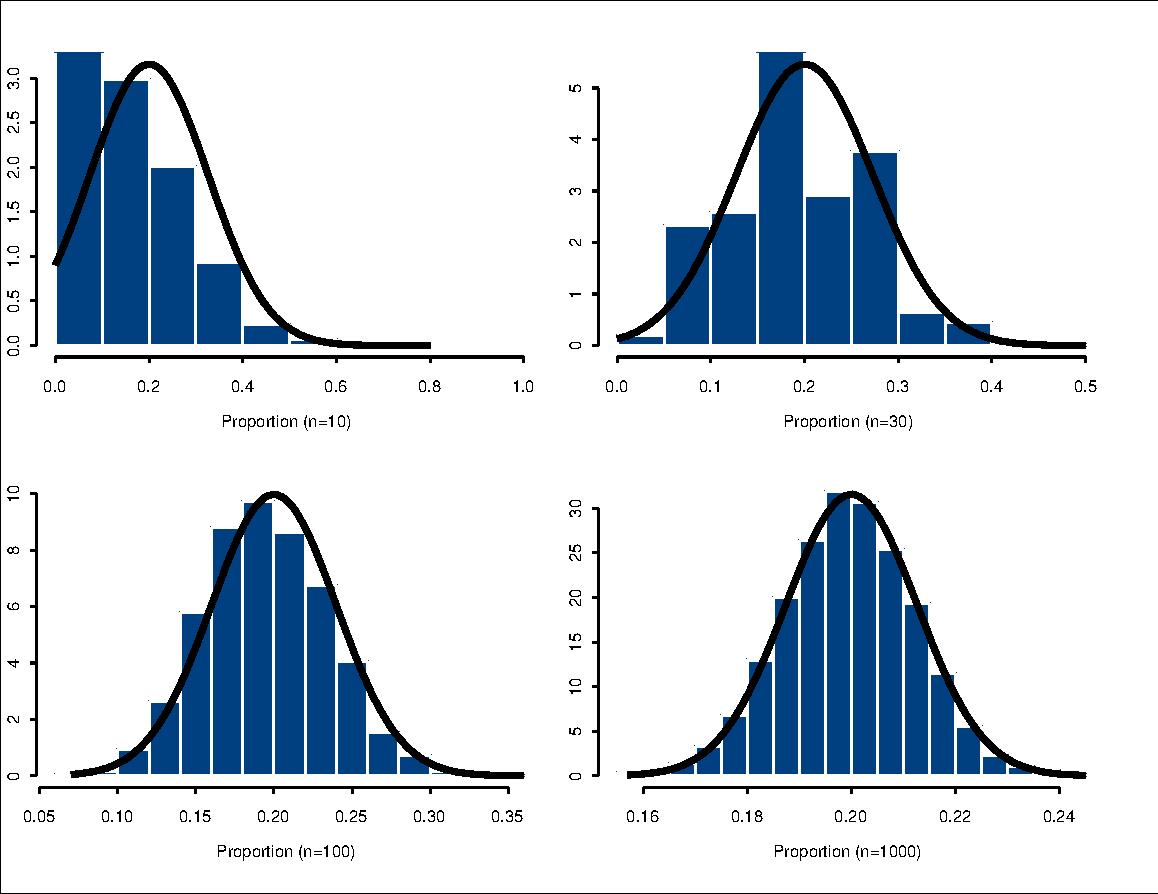
\includegraphics[width=14.00000cm]{sampld_p.pdf}
\caption{\label{fig:f-cltbin} Illustration of the Central Limit Theorem for
the sample proportion of a dichotomous variable. Each plot shows the
histogram of the sample proportions \(\hat{\pi}\) calculated for 5000
samples simulated from a population distribution with proportion
\(\pi=0.2\), together with the normal curve with mean \(\pi\) and
variance \(\pi(1-\pi)/n\). The samples sizes \(n\) are 10, 30, 100 and
1000.}
\end{figure}

The variability of the sampling distribution will again depend on \(n\).
In Figure \ref{fig:f-cltbin}, the observed range of values of
\(\hat{\pi}\) decreases substantially as \(n\) increases. When \(n=10\),
values of between about 0 and 0.4 are quite common, whereas with
\(n=1000\), essentially all of the samples give \(\hat{\pi}\) between
about 0.16 and 0.24, and a large majority are between 0.18 and 0.22.
Thus increasing the sample size will again increase the precision with
which we can estimate \(\pi\), and decrease the uncertainty in inference
about its true value.

The Central Limit Theorem is, with some additional results, the
justification for the standard normal sampling distribution used for
tests and confidence intervals for proportions in Chapter \ref{c-probs}.
The conditions for sample sizes mentioned there (at the beginning of
Section \ref{ss-probs-test1sample-samplingd} and \ref{s-probs-2samples})
again derive from conditions for the CLT to be adequate. The same is
also ultimately true for the \(\chi^{2}\) distribution and conditions
for the \(\chi^{2}\) test in Chapter \ref{c-tables}. Results like these,
and many others, explain the central importance of the CLT in
statistical methodology.

\chapter{Analysis of population means}\label{c-means}

\section{Introduction and examples}\label{s-means-intro}

This chapter introduces some basic methods of analysis for continuous,
interval-level variables. The main focus is on statistical inference on
population \emph{means} of such variables, but some new methods of
descriptive statistics are also described. The discussion draws on the
general ideas that have already been explaned for inference in Chapters
\ref{c-tables} and \ref{c-probs}, and for continuous distributions in
Chapter \ref{c-contd}. Few if any new concepts thus need to be
introduced here. Instead, this chapter can focus on describing the
specifics of these very commonly used methods for continuous variables.

As in Chapter \ref{c-probs}, questions on both a single group and on
comparisons between two groups are discussed here. Now, however, the
main focus is on the two-group case. There we treat the group as the
explanatory variable \(X\) and the continuous variable of interest as
the response variable \(Y\), and assess the possible associations
between \(X\) and \(Y\) by comparing the distributions (and especially
the means) of \(Y\) in the two groups.

The following five examples will be used for illustration throughout
this chapter. Summary statistics for them are shown in Table
\ref{tab:t-groupex}.

\paragraph{Example 7.1: Survey data on diet}\label{p-ex71}

The National Diet and Nutrition Survey of adults aged 19--64 living in
private households in Great Britain was carried out in
2000--01\footnote{ESS Round 5: European Social Survey Round 5 Data
  (2010). Data file edition 2.0. Norwegian Social Science Data Services,
  Norway � Data Archive and distributor of ESS data. The full data can
  be obtained from \texttt{http://ess.nsd.uib.no/ess/round5/}.}. One
part of the survey was a food diary where the respondents recorded all
food and drink they consumed in a seven-day period. We consider two
variables derived from the diary: the consumption of fruit and
vegetables in portions (of 400g) per day (with mean in the sample of
size \(n=1724\) of \(\bar{Y}=2.8\), and standard deviation \(s=2.15\)),
and the percentage of daily food energy intake obtained from fat and
fatty acids (\(n=1724\), \(\bar{Y}=35.3\), and \(s=6.11\)).

\begin{longtable}[]{@{}lrrrr@{}}
\caption{\label{tab:t-groupex} Examples of analyses of population means used
in Chapter \ref{c-means}. Here \(n\) and \(\bar{Y}\) denote the sample
size and sample mean respectively, in the two-group examples 7.2--7.5
separately for the two groups. ``Diff.'' denotes the between-group
difference of means, and \(s\) is the sample standard deviation of the
response variable \(Y\) for the whole sample (Example 7.1), of the
response variable within each group (Examples 7.2 and 7.3), or of the
within-pair differences (Examples 7.4 and 7.5).}\tabularnewline
\toprule
\begin{minipage}[b]{0.55\columnwidth}\raggedright\strut
\textbf{One sample}\strut
\end{minipage} & \begin{minipage}[b]{0.06\columnwidth}\raggedleft\strut
\(n\)\strut
\end{minipage} & \begin{minipage}[b]{0.10\columnwidth}\raggedleft\strut
\(\bar{Y}\)\strut
\end{minipage} & \begin{minipage}[b]{0.07\columnwidth}\raggedleft\strut
\(s\)\strut
\end{minipage} & \begin{minipage}[b]{0.08\columnwidth}\raggedleft\strut
Diff.\strut
\end{minipage}\tabularnewline
\midrule
\endfirsthead
\toprule
\begin{minipage}[b]{0.55\columnwidth}\raggedright\strut
\textbf{One sample}\strut
\end{minipage} & \begin{minipage}[b]{0.06\columnwidth}\raggedleft\strut
\(n\)\strut
\end{minipage} & \begin{minipage}[b]{0.10\columnwidth}\raggedleft\strut
\(\bar{Y}\)\strut
\end{minipage} & \begin{minipage}[b]{0.07\columnwidth}\raggedleft\strut
\(s\)\strut
\end{minipage} & \begin{minipage}[b]{0.08\columnwidth}\raggedleft\strut
Diff.\strut
\end{minipage}\tabularnewline
\midrule
\endhead
\begin{minipage}[t]{0.55\columnwidth}\raggedright\strut
\emph{Example 7.1: Variables from the National Diet and Nutrition
Survey}\strut
\end{minipage} & \begin{minipage}[t]{0.06\columnwidth}\raggedleft\strut
\strut
\end{minipage} & \begin{minipage}[t]{0.10\columnwidth}\raggedleft\strut
\strut
\end{minipage} & \begin{minipage}[t]{0.07\columnwidth}\raggedleft\strut
\strut
\end{minipage} & \begin{minipage}[t]{0.08\columnwidth}\raggedleft\strut
\strut
\end{minipage}\tabularnewline
\begin{minipage}[t]{0.55\columnwidth}\raggedright\strut
~~Fruit and vegetable consumption (400g portions)\strut
\end{minipage} & \begin{minipage}[t]{0.06\columnwidth}\raggedleft\strut
1724\strut
\end{minipage} & \begin{minipage}[t]{0.10\columnwidth}\raggedleft\strut
2.8\strut
\end{minipage} & \begin{minipage}[t]{0.07\columnwidth}\raggedleft\strut
2.15\strut
\end{minipage} & \begin{minipage}[t]{0.08\columnwidth}\raggedleft\strut
\strut
\end{minipage}\tabularnewline
\begin{minipage}[t]{0.55\columnwidth}\raggedright\strut
~~Total energy intake from fat (\%) \newline\strut
\end{minipage} & \begin{minipage}[t]{0.06\columnwidth}\raggedleft\strut
1724\strut
\end{minipage} & \begin{minipage}[t]{0.10\columnwidth}\raggedleft\strut
35.3\strut
\end{minipage} & \begin{minipage}[t]{0.07\columnwidth}\raggedleft\strut
6.11\strut
\end{minipage} & \begin{minipage}[t]{0.08\columnwidth}\raggedleft\strut
\strut
\end{minipage}\tabularnewline
\begin{minipage}[t]{0.55\columnwidth}\raggedright\strut
\textbf{Two independent samples}\strut
\end{minipage} & \begin{minipage}[t]{0.06\columnwidth}\raggedleft\strut
\strut
\end{minipage} & \begin{minipage}[t]{0.10\columnwidth}\raggedleft\strut
\strut
\end{minipage} & \begin{minipage}[t]{0.07\columnwidth}\raggedleft\strut
\strut
\end{minipage} & \begin{minipage}[t]{0.08\columnwidth}\raggedleft\strut
\strut
\end{minipage}\tabularnewline
\begin{minipage}[t]{0.55\columnwidth}\raggedright\strut
\emph{Example 7.2: Average weekly hours spent on housework}\strut
\end{minipage} & \begin{minipage}[t]{0.06\columnwidth}\raggedleft\strut
\strut
\end{minipage} & \begin{minipage}[t]{0.10\columnwidth}\raggedleft\strut
\strut
\end{minipage} & \begin{minipage}[t]{0.07\columnwidth}\raggedleft\strut
\strut
\end{minipage} & \begin{minipage}[t]{0.08\columnwidth}\raggedleft\strut
\strut
\end{minipage}\tabularnewline
\begin{minipage}[t]{0.55\columnwidth}\raggedright\strut
~~Men\strut
\end{minipage} & \begin{minipage}[t]{0.06\columnwidth}\raggedleft\strut
635\strut
\end{minipage} & \begin{minipage}[t]{0.10\columnwidth}\raggedleft\strut
7.33\strut
\end{minipage} & \begin{minipage}[t]{0.07\columnwidth}\raggedleft\strut
5.53\strut
\end{minipage} & \begin{minipage}[t]{0.08\columnwidth}\raggedleft\strut
\strut
\end{minipage}\tabularnewline
\begin{minipage}[t]{0.55\columnwidth}\raggedright\strut
~~Women \newline\strut
\end{minipage} & \begin{minipage}[t]{0.06\columnwidth}\raggedleft\strut
469\strut
\end{minipage} & \begin{minipage}[t]{0.10\columnwidth}\raggedleft\strut
8.49\strut
\end{minipage} & \begin{minipage}[t]{0.07\columnwidth}\raggedleft\strut
6.14\strut
\end{minipage} & \begin{minipage}[t]{0.08\columnwidth}\raggedleft\strut
1.16\strut
\end{minipage}\tabularnewline
\begin{minipage}[t]{0.55\columnwidth}\raggedright\strut
\emph{Example 7.3: Perceived friendliness of a police officer}\strut
\end{minipage} & \begin{minipage}[t]{0.06\columnwidth}\raggedleft\strut
\strut
\end{minipage} & \begin{minipage}[t]{0.10\columnwidth}\raggedleft\strut
\strut
\end{minipage} & \begin{minipage}[t]{0.07\columnwidth}\raggedleft\strut
\strut
\end{minipage} & \begin{minipage}[t]{0.08\columnwidth}\raggedleft\strut
\strut
\end{minipage}\tabularnewline
\begin{minipage}[t]{0.55\columnwidth}\raggedright\strut
~~No sunglasses\strut
\end{minipage} & \begin{minipage}[t]{0.06\columnwidth}\raggedleft\strut
67\strut
\end{minipage} & \begin{minipage}[t]{0.10\columnwidth}\raggedleft\strut
8.23\strut
\end{minipage} & \begin{minipage}[t]{0.07\columnwidth}\raggedleft\strut
2.39\strut
\end{minipage} & \begin{minipage}[t]{0.08\columnwidth}\raggedleft\strut
\strut
\end{minipage}\tabularnewline
\begin{minipage}[t]{0.55\columnwidth}\raggedright\strut
~~Sunglasses \newline\strut
\end{minipage} & \begin{minipage}[t]{0.06\columnwidth}\raggedleft\strut
66\strut
\end{minipage} & \begin{minipage}[t]{0.10\columnwidth}\raggedleft\strut
6.49\strut
\end{minipage} & \begin{minipage}[t]{0.07\columnwidth}\raggedleft\strut
2.01\strut
\end{minipage} & \begin{minipage}[t]{0.08\columnwidth}\raggedleft\strut
-1.74\strut
\end{minipage}\tabularnewline
\begin{minipage}[t]{0.55\columnwidth}\raggedright\strut
\textbf{Two dependent samples}\strut
\end{minipage} & \begin{minipage}[t]{0.06\columnwidth}\raggedleft\strut
\strut
\end{minipage} & \begin{minipage}[t]{0.10\columnwidth}\raggedleft\strut
\strut
\end{minipage} & \begin{minipage}[t]{0.07\columnwidth}\raggedleft\strut
\strut
\end{minipage} & \begin{minipage}[t]{0.08\columnwidth}\raggedleft\strut
\strut
\end{minipage}\tabularnewline
\begin{minipage}[t]{0.55\columnwidth}\raggedright\strut
\emph{Example 7.4: Father's personal well-being}\strut
\end{minipage} & \begin{minipage}[t]{0.06\columnwidth}\raggedleft\strut
\strut
\end{minipage} & \begin{minipage}[t]{0.10\columnwidth}\raggedleft\strut
\strut
\end{minipage} & \begin{minipage}[t]{0.07\columnwidth}\raggedleft\strut
\strut
\end{minipage} & \begin{minipage}[t]{0.08\columnwidth}\raggedleft\strut
\strut
\end{minipage}\tabularnewline
\begin{minipage}[t]{0.55\columnwidth}\raggedright\strut
~~Sixth month of wife's pregnancy\strut
\end{minipage} & \begin{minipage}[t]{0.06\columnwidth}\raggedleft\strut
109\strut
\end{minipage} & \begin{minipage}[t]{0.10\columnwidth}\raggedleft\strut
30.69\strut
\end{minipage} & \begin{minipage}[t]{0.07\columnwidth}\raggedleft\strut
\strut
\end{minipage} & \begin{minipage}[t]{0.08\columnwidth}\raggedleft\strut
\strut
\end{minipage}\tabularnewline
\begin{minipage}[t]{0.55\columnwidth}\raggedright\strut
~~One month after the birth \newline\strut
\end{minipage} & \begin{minipage}[t]{0.06\columnwidth}\raggedleft\strut
109\strut
\end{minipage} & \begin{minipage}[t]{0.10\columnwidth}\raggedleft\strut
30.77\strut
\end{minipage} & \begin{minipage}[t]{0.07\columnwidth}\raggedleft\strut
2.58\strut
\end{minipage} & \begin{minipage}[t]{0.08\columnwidth}\raggedleft\strut
0.08\strut
\end{minipage}\tabularnewline
\begin{minipage}[t]{0.55\columnwidth}\raggedright\strut
\emph{Example 7.5: Traffic flows on successive Fridays}\strut
\end{minipage} & \begin{minipage}[t]{0.06\columnwidth}\raggedleft\strut
\strut
\end{minipage} & \begin{minipage}[t]{0.10\columnwidth}\raggedleft\strut
\strut
\end{minipage} & \begin{minipage}[t]{0.07\columnwidth}\raggedleft\strut
\strut
\end{minipage} & \begin{minipage}[t]{0.08\columnwidth}\raggedleft\strut
\strut
\end{minipage}\tabularnewline
\begin{minipage}[t]{0.55\columnwidth}\raggedright\strut
~~Friday the 6th\strut
\end{minipage} & \begin{minipage}[t]{0.06\columnwidth}\raggedleft\strut
10\strut
\end{minipage} & \begin{minipage}[t]{0.10\columnwidth}\raggedleft\strut
128,385\strut
\end{minipage} & \begin{minipage}[t]{0.07\columnwidth}\raggedleft\strut
\strut
\end{minipage} & \begin{minipage}[t]{0.08\columnwidth}\raggedleft\strut
\strut
\end{minipage}\tabularnewline
\begin{minipage}[t]{0.55\columnwidth}\raggedright\strut
~~Friday the 13th\strut
\end{minipage} & \begin{minipage}[t]{0.06\columnwidth}\raggedleft\strut
10\strut
\end{minipage} & \begin{minipage}[t]{0.10\columnwidth}\raggedleft\strut
126,550\strut
\end{minipage} & \begin{minipage}[t]{0.07\columnwidth}\raggedleft\strut
1176\strut
\end{minipage} & \begin{minipage}[t]{0.08\columnwidth}\raggedleft\strut
-1835\strut
\end{minipage}\tabularnewline
\bottomrule
\end{longtable}

\paragraph{Example 7.2: Housework by men and women}\label{p-ex72}

This example uses data from the 12th wave of the British Household Panel
Survey (BHPS), collected in 2002. BHPS is an ongoing survey of UK
households, measuring a range of socioeconomic variables. One of the
questions in 2002 was

\emph{``About how many hours do you spend on housework in an average
week, such as time spent cooking, cleaning and doing the laundry?''}

The response to this question (recorded in whole hours) will be the
response variable \(Y\), and the respondent's sex will be the
explanatory variable \(X\). We consider only those respondents who were
less than 65 years old at the time of the interview and who lived in
single-person households (thus the comparisons considered here will not
involve questions of the division of domestic work within
families)\footnote{The data were obtained from
  \url{http://data.london.gov.uk/datastore/package/london-borough-profiles}.

  \noindentIf you download the ``Profiles in Excel'' workbook, you will
  find that one of the pages contains a map of the boroughs, and a tool
  for visualising the data on that map. A regular map of the boroughs
  can be found at for example at

  \url{http://www.londoncouncils.gov.uk/londonfacts/londonlocalgovernment/londonmapandlinks/default.htm}.}.

We can indicate summary statistics separately for the two groups by
using subscripts 1 for men and 2 for women (for example). The sample
sizes are \(n_{1}=635\) for men and \(n_{2}=469\) for women, and the
sample means of \(Y\) are \(\bar{Y}_{1}=7.33\) and \(\bar{Y}_{2}=8.49\).
These and the sample standard deviations \(s_{1}\) and \(s_{2}\) are
also shown in Table \ref{tab:t-groupex}.

\paragraph{Example 7.3: Eye contact and perceived friendliness of police
officers}\label{p-ex73}

This example is based on an experiment conducted to examine the effects
of some aspects of the appearance and behaviour of police officers on
how members of the public perceive their encounters with the
police\footnote{The data can be obtained from
  \texttt{http://www3.norc.org/gss+website/}, which gives further
  information on the survey, including the full text of the
  questionnaires.}. The subjects of the study were 133 people stopped by
the Traffic Patrol Division of a detachment of the Royal Canadian
Mounted Police. When talking to the driver who had been stopped, the
police officer either wore reflective sunglasses which hid his eyes, or
wore no glasses at all, thus permitting eye contact with the respondent.
These two conditions define the explanatory variable \(X\), coded 1 if
the officer wore no glasses and 2 if he wore sunglasses. The choice of
whether sunglasses were worn was made at random before a driver was
stopped.

While the police officer went back to his car to write out a report, a
researcher asked the respondent some further questions, one of which is
used here as the response variable \(Y\). It is a measure of the
respondent's perception of the friendliness of the police officer,
measured on a 10-point scale where large values indicate high levels of
friendliness.

The article describing the experiment does not report all the summary
statistics needed for our purposes. The statistics shown in Table
\ref{tab:t-groupex} have thus been partially made up for use here. They
are, however, consistent with the real results from the study. In
particular, the direction and statistical significance of the difference
between \(\bar{Y}_{2}\) and \(\bar{Y}_{1}\) are the same as those in the
published report.

\hypertarget{p-dependentex}{\paragraph{Example 7.4: Transition to
parenthood}\label{p-dependentex}}

In a study of the stresses and feelings associated with parenthood, 109
couples expecting their first child were interviewed before and after
the birth of the baby.\footnote{ESS Round 5: European Social Survey
  Round 5 Data (2010). Data file edition 2.0. Norwegian Social Science
  Data Services, Norway � Data Archive and distributor of ESS data. The
  full data can be obtained from
  \texttt{http://ess.nsd.uib.no/ess/round5/}.} Here we consider only
data for the fathers, and only one of the variables measured in the
study. This variable is a measure of personal well-being, obtained from
a seven-item attitude scale, where larger values indicate higher levels
of well-being. Measurements of it were obtained for each father at three
time points: when the mother was six months pregnant, one month after
the birth of the baby, and six months after the birth. Here we will use
only the first two of the measurements. The response variable \(Y\) will
thus be the measure of personal well-being, and the explanatory variable
\(X\) will be the time of measurement (sixth month of the pregnancy or
one month after the birth). The means of \(Y\) at the two times are
shown in Table \ref{tab:t-groupex}. As in Example 7.3, not all of the
numbers needed here were given in the original article. Specifically,
the standard error of the difference in Table \ref{tab:t-groupex} has
been made up in such a way that the results of a significance test for
the mean difference agree with those in the article.

\hypertarget{p-ex75}{\paragraph{Example 7.5: Traffic patterns on Friday
the 13th}\label{p-ex75}}

A common superstition regards the 13th day of any month falling on a
Friday as a particularly unlucky day. In a study examining the possible
effects of this belief on people's behaviour\footnote{Strictly speaking,
  the analysis should incorporate sampling weights (variable
  \emph{DWEIGHT}) to adjust for different sampling probabilities for
  different types of respondents. Here the weights are ignored. Using
  them would not change the main conclusions for these variables.}, data
were obtained on the numbers of vehicles travelling between junctions 7
and 8 and junctions 9 and 10 on the M25 motorway around London during
every Friday the 13th in 1990--92. For comparison, the same numbers were
also recorded during the previous Friday (i.e.~the 6th) in each case.
There are only ten such pairs here, and the full data set is shown in
Table \ref{tab:t-F13}. Here the explanatory variable \(X\) indicates
whether a day is Friday the 6th (coded as 1) or Friday the 13th (coded
as 2), and the response variable is the number of vehicles travelling
between two junctions.

\begin{longtable}[]{@{}llrrr@{}}
\caption{\label{tab:t-F13} Data for Example 7.5: Traffic flows between
junctions of the M25 on each Friday the 6th and Friday the 13th in
1990-92.}\tabularnewline
\toprule
Date & Junctions & Friday the 6th & Friday the 13th &
Difference\tabularnewline
\midrule
\endfirsthead
\toprule
Date & Junctions & Friday the 6th & Friday the 13th &
Difference\tabularnewline
\midrule
\endhead
July 1990 & 7 to 8 & 139246 & 138548 & -698\tabularnewline
July 1990 & 9 to 10 & 134012 & 132908 & -1104\tabularnewline
September 1991 & 7 to 8 & 137055 & 136018 & -1037\tabularnewline
September 1991 & 9 to 10 & 133732 & 131843 & -1889\tabularnewline
December 1991 & 7 to 8 & 123552 & 121641 & -1911\tabularnewline
December 1991 & 9 to 10 & 121139 & 118723 & -2416\tabularnewline
March 1992 & 7 to 8 & 128293 & 125532 & -2761\tabularnewline
March 1992 & 9 to 10 & 124631 & 120249 & -4382\tabularnewline
November 1992 & 7 to 8 & 124609 & 122770 & -1839\tabularnewline
November 1992 & 9 to 10 & 117584 & 117263 & -321\tabularnewline
\bottomrule
\end{longtable}

In each of these cases, we will regard the variable of interest \(Y\) as
a continuous, interval-level variable. The five examples illustrate
three different situations considered in this chapter. Example 7.1
includes two separate \(Y\)-variables (consumption of fruit and
vegetables, and fat intake), each of which is considered for a single
population. Questions of interest are about the mean of the variable in
the population. This is analogous to the one-group questions on
proportions in Sections \ref{s-probs-test1sample} and
\ref{s-probs-1sampleci}. In this chapter the one-group case is discussed
only relatively briefly, in Section \ref{s-means-1sample}.

The main focus here is on the case illustrated by Examples 7.2 and 7.3.
These involve samples of a response variable (hours of housework, or
preceived friendliness) from two groups (men and women, or police with
or without sunglasses). We are then interested in comparing the
distributions, and especially the means, of the response variable
between the groups. This case will be discussed first. Descriptive
statistics for it are described in Section \ref{s-means-descr}, and
statistical inference in Section \ref{s-means-inference}.

Finally, examples 7.4 and 7.5 also involve comparisons between two
groups, but of a slightly different kind than examples 7.2 and 7.3. The
two types of cases differ in the nature of the two samples (groups)
being compared. \label{p-depsamples} In Examples 7.2 and 7.3, the
samples can be considered to be \textbf{independent}. What this claim
means will be discussed briefly later; informally, it is justified in
these examples because the subjects in the two groups are separate and
unrelated individuals. In Examples 7.4 and 7.5, in contrast, the samples
(before and after the birth of a child, or two successive Fridays) must
be considered \textbf{dependent}, essentially because they concern
measurements on the same units at two distinct times. This case is
discussed in Section \ref{s-means-dependent}.

In each of the four two-group examples we are primarily interested in
questions about possible association between the group variable \(X\)
and the response variable \(Y\). As before, this is the question of
whether the conditional distributions of \(Y\) are different at the two
levels of \(X\). There is thus an association between \(X\) and \(Y\) if

\begin{itemize}
\item
  Example 7.2: The distribution of hours of housework is different for
  men than for women.
\item
  Example 7.3: The distribution of perceptions of a police officer's
  friendliness is different when he is wearing mirrored sunglasses than
  when he is not.
\item
  Example 7.4: The distribution of measurements of personal well-being
  is different at the sixth month of the pregnancy than one month after
  the birth.
\item
  Example 7.5: The distributions of the numbers of cars on the motorway
  differ between Friday the 6th and the following Friday the 13th.
\end{itemize}

We denote the two values of \(X\), i.e.~the two groups, by 1 and 2. The
mean of the population distribution of \(Y\) given \(X=1\) will be
denoted \(\mu_{1}\) and the standard deviation \(\sigma_{1}\), and the
mean and standard deviation of the population distribution given \(X=2\)
are denoted \(\mu_{2}\) and \(\sigma_{2}\) similarly. The corresponding
sample quantities are the conditional sample means \(\bar{Y}_{1}\) and
\(\bar{Y}_{2}\) and sample standard deviations \(s_{1}\) and \(s_{2}\).
For inference, we will focus on the population difference
\(\Delta=\mu_{2}-\mu_{1}\) which is estimated by the sample difference
\(\hat{\Delta}=\bar{Y}_{2}-\bar{Y}_{1}\). Some of the descriptive
methods described in Section \ref{s-means-descr}, on the other hand,
also aim to summarise and compare other aspects of the two conditional
sample distributions.

\section{Descriptive statistics for comparisons of
groups}\label{s-means-descr}

\subsection{Graphical methods of comparing sample
distributions}\label{ss-means-descr-graphs}

There is an association between the group variable \(X\) and the
response variable \(Y\) if the distributions of \(Y\) in the two groups
are not the same. To determine the extent and nature of any such
association, we need to compare the two distributions. This section
describes methods of doing so for observed data, i.e.~for examining
associations in a sample. We begin with graphical methods which can be
used to detect differences in any aspects of the two distributions. We
then discuss some non-graphical summaries which compare specific aspects
of the sample distributions, especially their means.

Although the methods of \emph{inference} described later in this chapter
will be limited to the case where the group variable \(X\) is
dichotomous, many of the descriptive methods discussed below can just as
easily be applied when more than two groups are being compared. This
will be mentioned wherever appropriate. For inference in the
multiple-group case some of the methods discussed in Chapter
\ref{c-regression} are applicable.

In Section \ref{ss-descr1-1cont-graphs} we described four graphical
methods of summarizing the sample distribution of one continuous
variable \(Y\): the histogram, the stem and leaf plot, the frequency
polygon and the box plot. Each of these can be adapted for comparisons
of two or more distributions, although some more conveniently than
others. We illustrate the use three of the plots for this purpose, using
the comparison of housework hours in Example 7.2 for illustration. Stem
and leaf plots will not be shown, because they are less appropriate when
the sample sizes are as large as they are in this example.

Two sample distributions can be compared by displaying histograms of
them side by side, as shown in Figure \ref{fig:f-hworkpyramid}. This is
not a very common type of graph, and not ideal for visually comparing
the two distributions, because the bars to be compared (here for men
vs.~women) end at opposite ends of the plot. A better alternative is to
use frequency polygons. Since these represent a sample distribution by a
single line, it is easy to include two of them in the same plot, as
shown in Figure \ref{fig:f-hworkpolygons}. Finally, Figure
\ref{fig:f-twoboxplots} shows two boxplots of reported housework hours,
one for men and one for women.

The plots suggest that the distributions are quite similar for men and
women. In both groups, the largest proportion of respondents stated that
they do between 4 and 7 hours of housework a week. The distributions are
clearly positively skewed, since the reported number of hours was much
higher than average for a number of people (whereas less than zero hours
were of course not recorded for anyone). The proportions of observations
in categories including values 5, 10, 15, 20, 25 and 30 tend to be
relatively high, suggesting that many respondents chose to report their
answers in such round numbers. The box plots show that the median number
of hours is higher for women than for men (7 vs.~6 hours), and women's
responses have slightly less variation, as measured by both the IQR and
the range of the whiskers. Both distributions have several larger,
outlying observations (note that SPSS, which was used to produce Figure
\ref{fig:f-twoboxplots}, divides outliers into moderate and ``extreme''
ones; the latter are observations more than 3 IQR from the end of the
box, and are plotted with asterisks).

\begin{figure}[htbp]
\centering
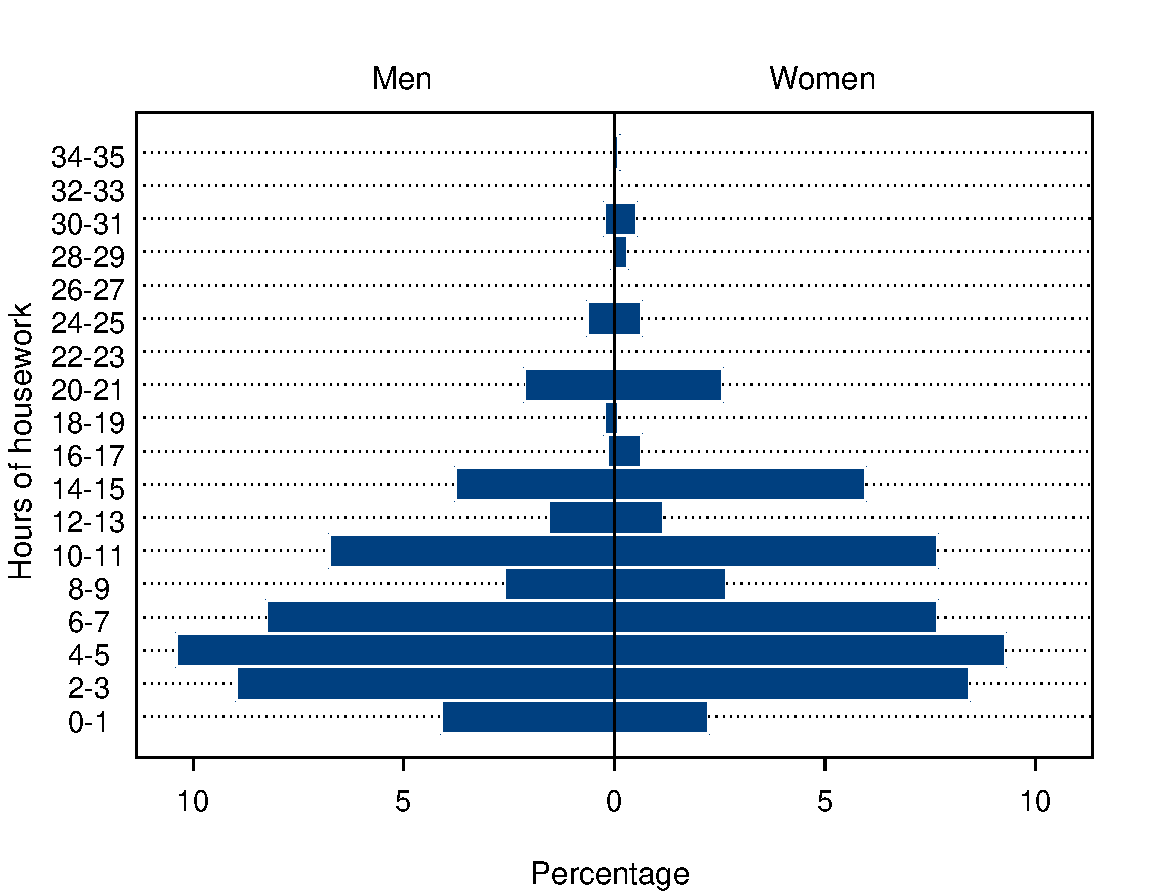
\includegraphics[width=13.00000cm]{hworkpyramid.pdf}
\caption{\label{fig:f-hworkpyramid} Histograms of the sample distributions
of reported weekly hours of housework in Example 7.2, separately for men
(\(n=635\)) and women (\(n=469\)).}
\end{figure}

\begin{figure}[htbp]
\centering
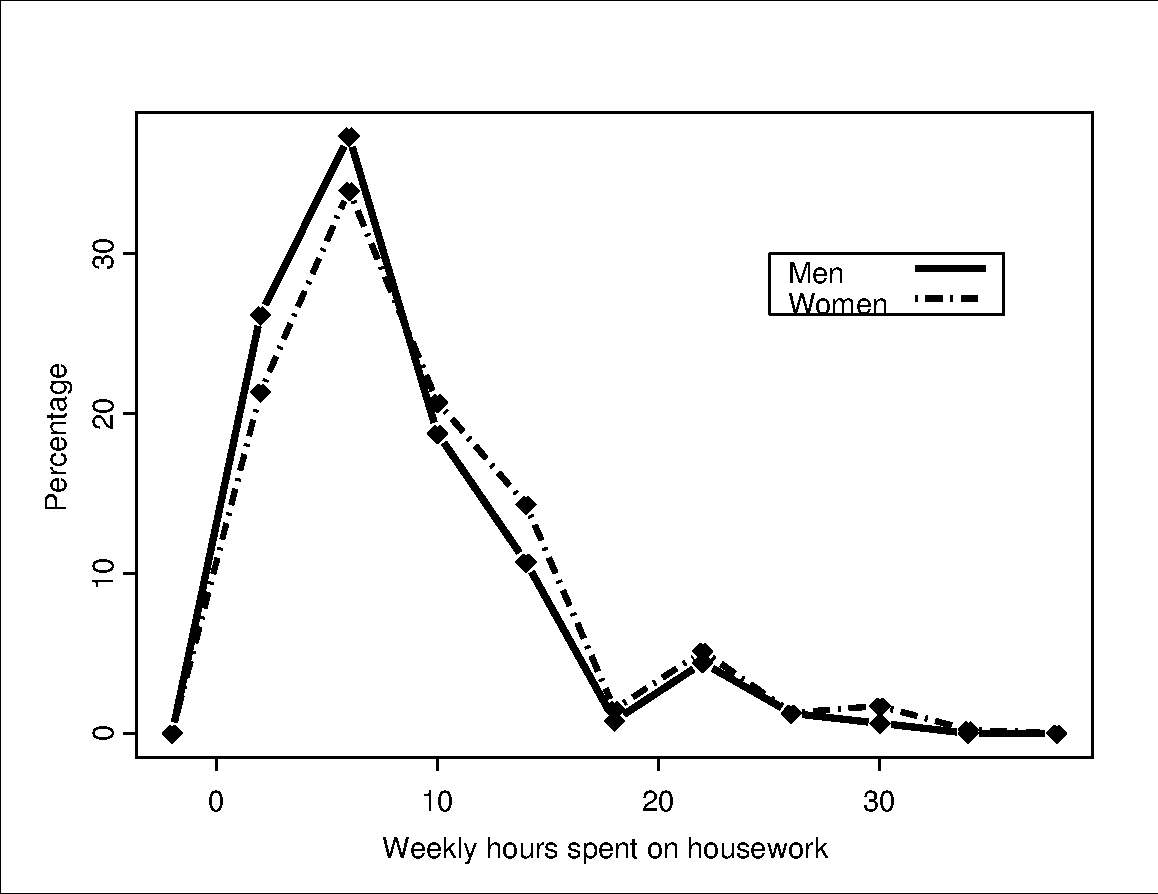
\includegraphics[width=11.50000cm]{hwork.pdf}
\caption{\label{fig:f-hworkpolygons} Frequency polygons of the sample
distributions of reported weekly hours of housework in Example 7.2,
separately for men and women. The points show the percentages of
observations in the intervals of 0--3, 4--7, \(\dots\), 32--35 hours
(plus zero percentages at each end of the curve).}
\end{figure}

\begin{figure}[htbp]
\centering
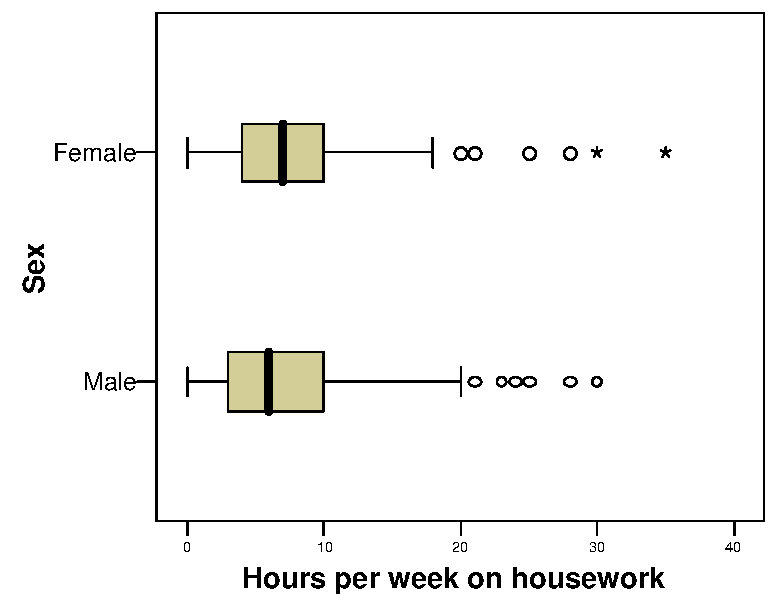
\includegraphics[width=11.00000cm]{twoboxplots.pdf}
\caption{\label{fig:f-twoboxplots} Box plots of the sample distributions of
reported weekly hours of housework in Example 7.2, separately for men
and women.}
\end{figure}

Figures \ref{fig:f-hworkpyramid}--\ref{fig:f-twoboxplots} also
illustrate an important general point about such comparisons. Typically
we focus on comparing \emph{means} of the conditional distributions.
Here the difference between the sample means is 1.16, i.e.~women in the
sample spend, on average, over an hour longer on housework per week than
men. The direction of the difference could also be guessed from Figure
\ref{fig:f-hworkpolygons}, which shows that somewhat smaller proportions
of women than of men report small numbers of hours, and larger
proportions of women report large numbers. This difference will later be
shown to be statistically significant, and it is also arguably
relatively large in a substantive sense.

However, it is equally important to note that the two distributions
summarized by the graphs are nevertheless largely similar. For example,
even though the mean is higher for women, there are clearly many women
who report spending hardly any time on housework, and many men who spend
a lot of time on it. In other words, the two distributions overlap to a
large extent. This obvious point is often somewhat neglected in public
discussions of differences between groups such as men and women or
different ethnic groups. It is not uncommon to see reports of research
indicating that (say) men have higher or lower values of something or
other then women. Such statements usually refer to differences of
averages, and are often clearly important and interesting. Less helpful,
however, is the tendency to discuss the differences almost as if the
corresponding distributions had no overlap at all, i.e.~as if \emph{all}
men were higher or lower in some characteristic than all women. This is
obviously hardly ever the case.

Box plots and frequency polygons can also be used to compare more than
two sample distributions. For example, the experimental conditions in
the study behind Example 7.3 actually involved not only whether or not a
police officer wore sunglasses, but also whether or not he wore a gun.
Distributions of perceived friendliness given all four combinations of
these two conditions could easily be summarized by drawing four box
plots or frequency polygons in the same plot, one for each experimental
condition.

\subsection{Comparing summary statistics}\label{ss-means-descr-tables}

Main features of sample distributions, such as their central tendencies
and variations, are described using the summary statistics introduced in
Section \ref{s-descr1-nums}. These too can be compared between groups.
Table \ref{tab:t-groupex} shows such statistics for the examples of this
chapter. Tables like these are routinely reported for initial
description of data, even if more elaborate statistical methods are
later used.

Sometimes the association between two variables in a sample is
summarized in a single \emph{measure of association} calculated from the
data. This is especially convenient when both of the variables are
continuous (in which case the most common measure of association is
known as the \emph{correlation} coefficient). In this section we
consider as such a summary the difference
\(\hat{\Delta}=\bar{Y}_{2}-\bar{Y}_{1}\) of the sample means of \(Y\) in
the two groups. These differences are also shown in Table
\ref{tab:t-groupex}.

The difference of means is important because it is also the focus of the
most common methods of inference for two-group comparisons. For purely
descriptive purposes it may be as or more convenient to report some
other statistic. For example, the difference of means of 1.16 hours in
Example 7.2 could also be described in \emph{relative} terms by saying
that the women's average is about 16 per cent higher than the men's
average (because \(1.16/7.33=0.158\), i.e.~the difference represents
15.8 \% of the men's average).

\section{Inference for two means from independent
samples}\label{s-means-inference}

\subsection{Aims of the analysis}\label{ss-means-inference-intro}

Formulated as a statistical model in the sense discussed on page in
Section \ref{ss-contd-probdistrs-general}, the assumptions of the
analyses considered in this section are as follows:

\begin{enumerate}
\def\labelenumi{\arabic{enumi}.}
\item
  \label{p-2sample} We have a sample of \(n_{1}\) independent
  observations of a variable \(Y\) in group 1, which have a population
  distribution with mean \(\mu_{1}\) and standard deviation
  \(\sigma_{1}\).
\item
  We have a sample of \(n_{2}\) independent observations of \(Y\) in
  group 2, which have a population distribution with mean \(\mu_{2}\)
  and standard deviation \(\sigma_{2}\).
\item
  The two samples are independent, in the sense discussed following
  \protect\hyperlink{p-ex75}{Example 7.5}.
\item
  For now, we further assume that the population standard deviations
  \(\sigma_{1}\) and \(\sigma_{2}\) are equal, with a common value
  denoted by \(\sigma\). This relatively minor assumption will be
  discussed further in Section \ref{ss-means-inference-variants}.
\end{enumerate}

We could have stated the starting points of the analyses in Chapters
\ref{c-tables} and \ref{c-probs} also in such formal terms. It is not
absolutely necessary to always do so, but we should at least remember
that any statistical analysis is based on some such model. In
particular, this helps to make it clear what our methods of analysis do
and do not assume, so that we may critically examine whether these
assumptions appear to be justified for the data at hand.

The model stated above does not require that the population
distributions of \(Y\) should have the form of any particular
probability distribution. It is often further assumed that these
distributions are normal distributions, but this is not essential.
Discussion of this question is postponed until Section
\ref{ss-means-inference-variants}.

The only new term in this model statement was the ``independent'' under
assumptions 1 and 2. This statistical term can be roughly translated as
``unrelated''. The condition can usually be regarded as satisfied when
the units of analysis are different entities, as in Examples 7.2 and 7.3
where the units within each group are distinct individual people. In
these examples the individuals in the two groups are also distinct, from
which it follows that the two \emph{samples} are independent as required
by assumption 3. The same assumption of independent observations is also
required by all of the methods described in Chapters \ref{c-tables} and
\ref{c-probs}, although we did not state this explicitly there.

This situation is illustrated by Example 7.2, where \(Y\) is the number
of hours a person spends doing housework in a week, and the two groups
are men (group 1) and women (group 2).

The quantity of main interest is here the difference of population means

\begin{equation} \Delta=\mu_{2}-\mu_{1}.
\label{eq:DeltaB} \end{equation}

In particular, if \(\Delta=0\), the population means in the two groups
are the same. If \(\Delta\ne 0\), they are not the same, which implies
that there is an association between \(Y\) and the group in the
population.

Inference on \(\Delta\) can be carried out using methods which are
straightforward modifications of the ones introduced first in Chapter
\ref{c-probs}. For significance testing, the null hypothesis of interest
is

\begin{equation}H_{0}: \; \Delta=0,
\label{eq:mH0a}\end{equation}

to be tested against a two-sided (\(H_{a}:\; \Delta\ne 0\)) or one-sided
(\(H_{a}:\; \Delta> 0\) or \(H_{a}:\; \Delta< 0\)) alternative
hypothesis. The test statistic used to test (\ref{eq:mH0a}) is again of
the form

\begin{equation}t=\frac{\hat{\Delta}}{\hat{\sigma}_{\hat{\Delta}}}
\label{eq:tma}\end{equation}

where \(\hat{\Delta}\) is a sample estimate of \(\Delta\), and
\(\hat{\sigma}_{\hat{\Delta}}\) its estimated standard error. Here the
statistic is conventionally labelled \(t\) rather than \(z\) and called
the \emph{t-test statistic} because sometimes the \(t\)-distribution
rather than the normal is used as its sampling distribution. This
possibility is discussed in Section \ref{ss-means-inference-variants},
and we can ignore it until then.

Confidence intervals for the differences \(\Delta\) are also of the
familiar form

\begin{equation}\hat{\Delta} \pm z_{\alpha/2}\, \hat{\sigma}_{\hat{\Delta}}
\label{eq:ciDpa}\end{equation}

where \(z_{\alpha/2}\) is the appropriate multiplier from the standard
normal distribution to obtain the required confidence level, e.g.
\(z_{0.025}=1.96\) for 95\% confidence intervals. The multiplier is
replaced with a slightly different one if the \(t\)-distribution is used
as the sampling distribution, as discussed in Section
\ref{ss-means-inference-variants}.

The details of these formulas in the case of two-sample inference on
means are described next, in Section \ref{ss-means-inference-test} for
the significance test and in Section \ref{ss-means-inference-ci} for the
confidence interval.

\subsection{\texorpdfstring{Significance testing: The two-sample
\(t\)-test}{Significance testing: The two-sample t-test}}\label{ss-means-inference-test}

For tests of the difference of means \(\Delta=\mu_{2}-\mu_{1}\) between
two population distributions, we consider the null hypothesis of no
difference

\begin{equation}H_{0}: \; \Delta=0.
\label{eq:H0m}\end{equation}

In the housework example, this is the hypothesis that average weekly
hours of housework in the population are the same for men and women. It
is tested against an alternative hypothesis, either the two-sided
alternative hypotheses

\begin{equation}H_{a}: \; \Delta\ne 0\label{eq:Hatwom}\end{equation}

or one of the one-sided alternative hypotheses
\[H_{a}:  \Delta> 0 \text{ or } H_{a}:  \Delta< 0\] In the discussion
below, we concentrate on the more common two-sided alternative.

The test statistic for testing (\ref{eq:H0m}) is of the general form
(\ref{eq:tma}). Here it depends on the data only through the sample
means \(\bar{Y}_{1}\) and \(\bar{Y}_{2}\) and sample variances
\(s_{1}^{2}\) and \(s_{2}^{2}\) of \(Y\) in the two groups. A point
estimate of \(\Delta\) is

\begin{equation}\hat{\Delta}=\bar{Y}_{2}-\bar{Y}_{1}.
\label{eq:Dhatmu}\end{equation}

In terms of the population parameters, the standard error of
\(\hat{\Delta}\) is

\begin{equation}\sigma_{\hat{\Delta}}=
\sqrt{\sigma^{2}_{\bar{Y}_{2}}+
\sigma^{2}_{\bar{Y}_{1}}}=
\sqrt{
\frac{\sigma^{2}_{2}}{n_{2}}+
\frac{\sigma^{2}_{1}}{n_{1}}
}.
\label{eq:sigmaDmu}\end{equation}

When we assume that the population standard deviations \(\sigma_{1}\)
and \(\sigma_{2}\) are equal, with a common value \(\sigma\),
(\ref{eq:sigmaDmu}) simplifies to

\begin{equation}\sigma_{\hat{\Delta}} =
\sigma\; \sqrt{
\frac{1}{n_{2}}+
\frac{1}{n_{1}}
}.
\label{eq:seDpop}\end{equation}

The formula of the test statistic uses an estimate of this standard
error, given by

\begin{equation}\hat{\sigma}_{\hat{\Delta}} =
\hat{\sigma} \; \sqrt{\frac{1}{n_{2}}+\frac{1}{n_{1}}}
\label{eq:seD2}\end{equation}

where \(\hat{\sigma}\) is an estimate of \(\sigma\), calculated from

\begin{equation}\hat{\sigma}=
\sqrt{\frac{(n_{2}-1)s^{2}_{2}+(n_{1}-1)s^{2}_{1}}{n_{1}+n_{2}-2}}.
\label{eq:sehatjoint}\end{equation}

Substituting (\ref{eq:Dhatmu}) and (\ref{eq:seD2}) into the general
formula (\ref{eq:tma}) gives the \textbf{two-sample t-test statistic for
means}

\begin{equation}t=
\frac{\bar{Y}_{2}-\bar{Y}_{1}}
{\hat{\sigma}\, \sqrt{1/n_{2}+1/n_{1}}}
\label{eq:ztestmuDb}\end{equation}

where \(\hat{\sigma}\) is given by (\ref{eq:sehatjoint}).

For an illustration of the calculations, consider again the housework
Example 7.2. Here, denoting men by 1 and women by 2, \(n_{1}=635\),
\(n_{2}=469\), \(\bar{Y}_{1}=7.33\), \(\bar{Y}_{2}=8.49\),
\(s_{1}=5.53\) and \(s_{2}=6.14\). The estimated mean difference is thus
\[\hat{\Delta}=\bar{Y}_{2}-\bar{Y}_{1}=8.49-7.33=1.16.\] The common
value of the population standard deviation \(\sigma\) is estimated from
(\ref{eq:sehatjoint}) as \[\begin{aligned}
\hat{\sigma}&=&
\sqrt{\frac{(n_{2}-1)s^{2}_{2}+(n_{1}-1)s^{2}_{1}}{n_{1}+n_{2}-2}}
=
\sqrt{\frac{(469-1) 6.14^{2}+(635-1) 5.53^{2}}{635+469-2}}\\
&=& \sqrt{33.604}=5.797\end{aligned}\] and the estimated standard error
of \(\hat{\Delta}\) is given by (\ref{eq:seD2}) as
\[\hat{\sigma}_{\hat{\Delta}} =
\hat{\sigma} \; \sqrt{\frac{1}{n_{2}}+\frac{1}{n_{1}}}
=5.797 \; \sqrt{\frac{1}{469}+\frac{1}{635}}=0.353.\] The value of the
t-test statistic (\ref{eq:ztestmuDb}) is then obtained as
\[t=\frac{1.16}{0.353}=3.29.\] These values and other quantities
explained later, as well as similar results for Example 7.3, are also
shown in Table \ref{tab:t-2testsY1}.

\begin{longtable}[]{@{}rrrrr@{}}
\caption{\label{tab:t-2testsY1} Results of tests and confidence intervals
for comparing means for two independent samples. For Example 7.2, the
difference of means is between women and men, and for Example 7.3, it is
between wearing and not wearing sunglasses. The test statistics and
confidence intervals are obtained under the assumption of equal
population standard deviations, and the \(P\)-values are for a test with
a two-sided alternative hypothesis. See the text for the definitions of
the statistics.}\tabularnewline
\toprule
\begin{minipage}[b]{0.28\columnwidth}\raggedleft\strut
\(\hat{\Delta}\)\strut
\end{minipage} & \begin{minipage}[b]{0.25\columnwidth}\raggedleft\strut
\(\hat{\sigma}_{\hat{\Delta}}\)\strut
\end{minipage} & \begin{minipage}[b]{0.08\columnwidth}\raggedleft\strut
\(t\)\strut
\end{minipage} & \begin{minipage}[b]{0.09\columnwidth}\raggedleft\strut
\(P\)-value\strut
\end{minipage} & \begin{minipage}[b]{0.14\columnwidth}\raggedleft\strut
95 \% C.I.\strut
\end{minipage}\tabularnewline
\midrule
\endfirsthead
\toprule
\begin{minipage}[b]{0.28\columnwidth}\raggedleft\strut
\(\hat{\Delta}\)\strut
\end{minipage} & \begin{minipage}[b]{0.25\columnwidth}\raggedleft\strut
\(\hat{\sigma}_{\hat{\Delta}}\)\strut
\end{minipage} & \begin{minipage}[b]{0.08\columnwidth}\raggedleft\strut
\(t\)\strut
\end{minipage} & \begin{minipage}[b]{0.09\columnwidth}\raggedleft\strut
\(P\)-value\strut
\end{minipage} & \begin{minipage}[b]{0.14\columnwidth}\raggedleft\strut
95 \% C.I.\strut
\end{minipage}\tabularnewline
\midrule
\endhead
\begin{minipage}[t]{0.28\columnwidth}\raggedleft\strut
Example 7.2: Average weekly hours spent on housework\strut
\end{minipage} & \begin{minipage}[t]{0.25\columnwidth}\raggedleft\strut
\strut
\end{minipage} & \begin{minipage}[t]{0.08\columnwidth}\raggedleft\strut
\strut
\end{minipage} & \begin{minipage}[t]{0.09\columnwidth}\raggedleft\strut
\strut
\end{minipage} & \begin{minipage}[t]{0.14\columnwidth}\raggedleft\strut
\strut
\end{minipage}\tabularnewline
\begin{minipage}[t]{0.28\columnwidth}\raggedleft\strut
1.16\strut
\end{minipage} & \begin{minipage}[t]{0.25\columnwidth}\raggedleft\strut
0.353\strut
\end{minipage} & \begin{minipage}[t]{0.08\columnwidth}\raggedleft\strut
3.29\strut
\end{minipage} & \begin{minipage}[t]{0.09\columnwidth}\raggedleft\strut
0.001\strut
\end{minipage} & \begin{minipage}[t]{0.14\columnwidth}\raggedleft\strut
(0.47; 1.85)\strut
\end{minipage}\tabularnewline
\begin{minipage}[t]{0.28\columnwidth}\raggedleft\strut
Example 7.3: Perceived friendliness of a police officer\strut
\end{minipage} & \begin{minipage}[t]{0.25\columnwidth}\raggedleft\strut
\strut
\end{minipage} & \begin{minipage}[t]{0.08\columnwidth}\raggedleft\strut
\strut
\end{minipage} & \begin{minipage}[t]{0.09\columnwidth}\raggedleft\strut
\strut
\end{minipage} & \begin{minipage}[t]{0.14\columnwidth}\raggedleft\strut
\strut
\end{minipage}\tabularnewline
\begin{minipage}[t]{0.28\columnwidth}\raggedleft\strut
\(-1.74\)\strut
\end{minipage} & \begin{minipage}[t]{0.25\columnwidth}\raggedleft\strut
0.383\strut
\end{minipage} & \begin{minipage}[t]{0.08\columnwidth}\raggedleft\strut
\(-4.55\)\strut
\end{minipage} & \begin{minipage}[t]{0.09\columnwidth}\raggedleft\strut
\(<0.001\)\strut
\end{minipage} & \begin{minipage}[t]{0.14\columnwidth}\raggedleft\strut
\((-2.49; -0.99)\)\strut
\end{minipage}\tabularnewline
\bottomrule
\end{longtable}

\label{p-spss2a} If necessary, calculations like these can be carried
out even with a pocket calculator. It is, however, much more convenient
to leave them to statistical software. Figure \ref{fig:f-spss2test}
shows SPSS output for the two-sample t-test for the housework data. The
first part of the table, labelled ``Group Statistics'', shows the sample
sizes \(n\), means \(\bar{Y}\) and standard deviations \(s\) separately
for the two groups. The quantity labelled ``Std.~Error Mean'' is
\(s/\sqrt{n}\). This is an estimate of the standard error of the sample
mean, which is the quantity \(\sigma/\sqrt{n}\) discussed in Section
\ref{s-contd-clt}.

The second part of the table in Figure \ref{fig:f-spss2test}, labelled
``Independent Samples Test'', gives results for the t-test itself. The
test considered here, which assumes a common population standard
deviation \(\sigma\) (and thus also variance \(\sigma^{2}\)), is found
on the row labelled ``Equal variances assumed''. The test statistic is
shown in the column labelled ``\(t\)'', and the difference
\(\hat{\Delta}=\bar{Y}_{2}-\bar{Y}_{1}\) and its standard error
\(\hat{\sigma}_{\hat{\Delta}}\) are shown in the ``Mean Difference'' and
``Std. Error Difference'' columns respectively. Note that the difference
(\(-1.16\)) has been calculated in SPSS between men and women rather
than vice versa as in Table \ref{tab:t-2testsY1}, but this will make no
difference to the conclusions from the test.

\begin{figure}[htbp]
\centering
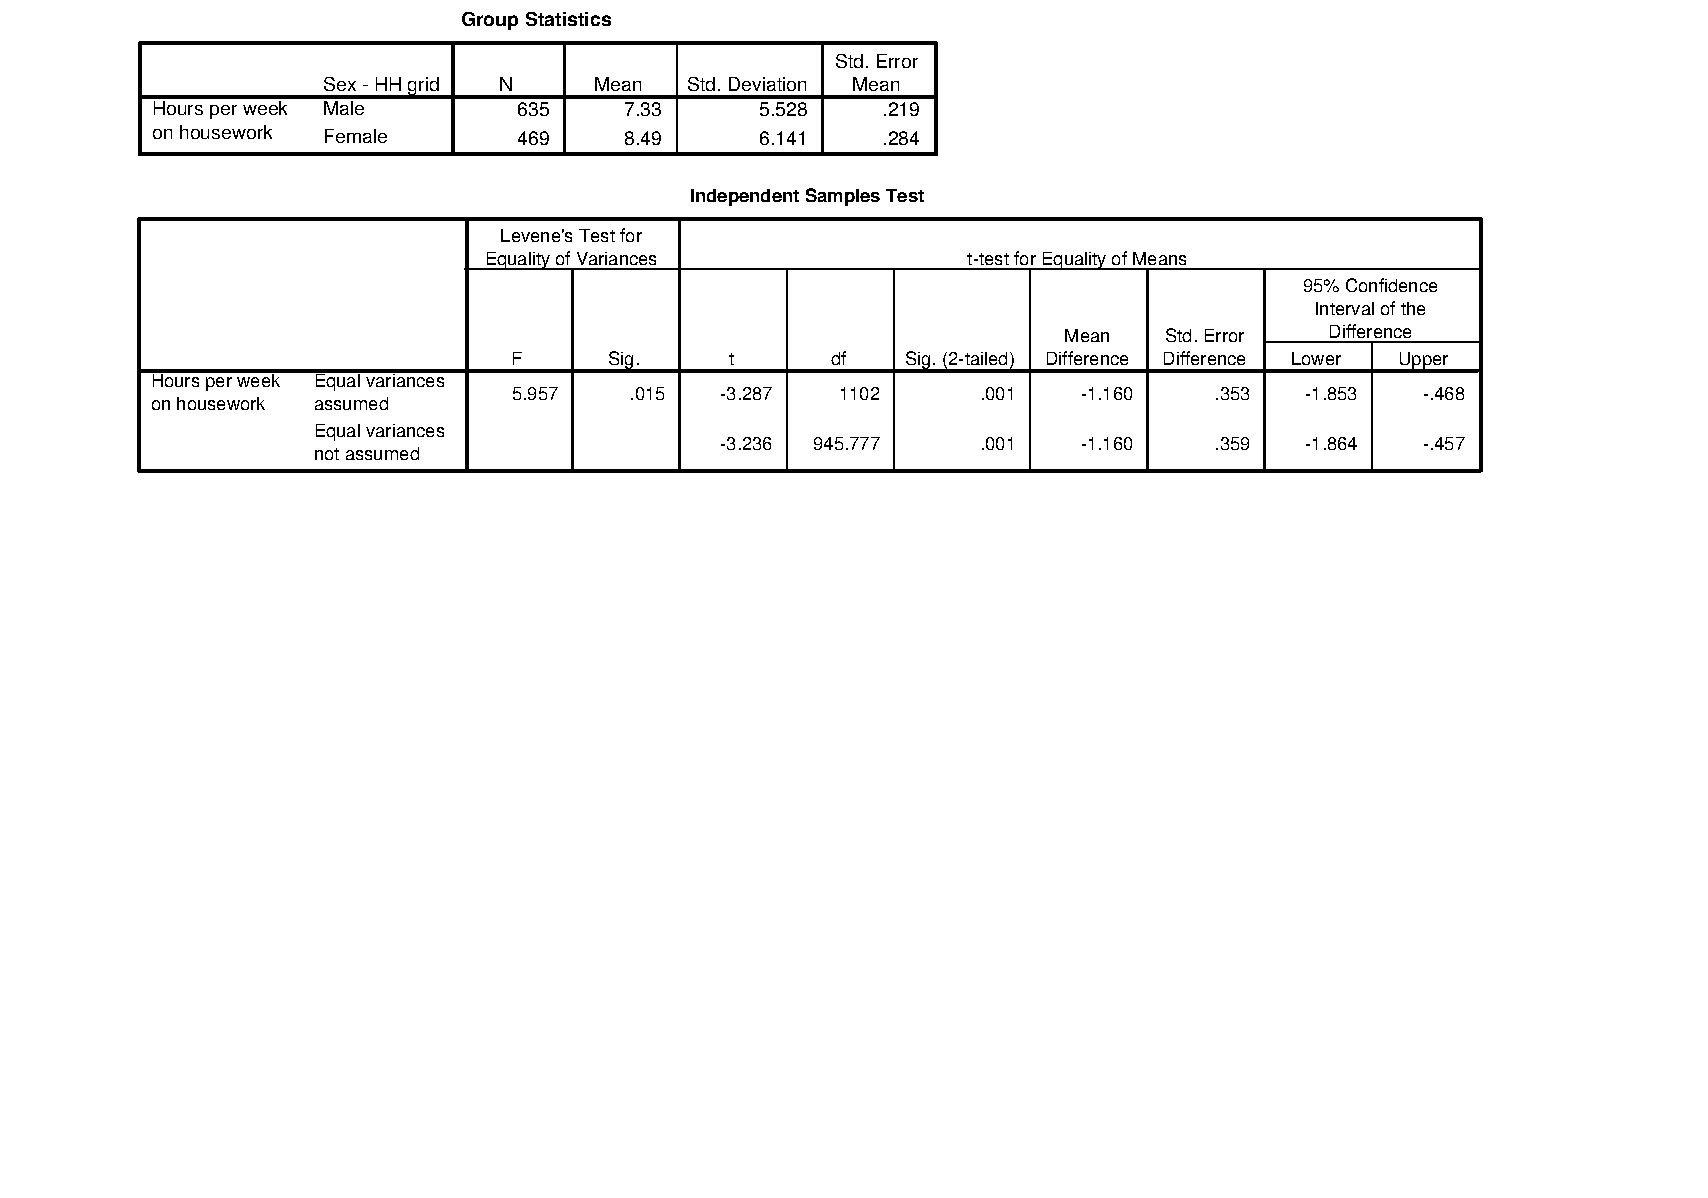
\includegraphics[height=20.00000cm]{spss2t.pdf}
\caption{\label{fig:f-spss2test} SPSS output for a two-sample \(t\)-test in
Example 7.2, comparing average weekly hours spent on housework between
men and women.}
\end{figure}

\label{p-ztestass} In the two-sample situation with assumptions 1--4 at
the beginning of Section \ref{ss-means-inference-intro}, the sampling
distribution of the t-test statistic (\ref{eq:ztestmuDb}) is
approximately a standard normal distribution when the null hypothesis
\(H_{0}: \; \Delta=\mu_{2}-\mu_{1}=0\) is true in the population and the
sample sizes are large enough. This is again a consequence of the
Central Limit Theorem. The requirement for ``large enough'' sample sizes
is fairly easy to satisfy. A good rule of thumb is that the sample sizes
\(n_{1}\) and \(n_{2}\) in the two groups should both be at least 20 for
the sampling distribution of the test statistic to be well enough
approximated by the standard normal distribution. In the housework
example we have data on 635 men and 469 women, so the sample sizes are
clearly large enough. A variant of the test which relaxes the condition
on the sample sizes is discussed in Section
\ref{ss-means-inference-variants} below.

The \(P\)-value of the test is calculated from this sampling
distribution in exactly the same way as for the tests of proportions in
Section \ref{ss-probs-test1sample-samplingd}. In the housework example
the value of the \(t\)-test statistic is \(t=3.29\). The \(P\)-value for
testing the null hypothesis against the two-sided alternative
(\ref{eq:Hatwom}) is then the probability, calculated from the standard
normal distribution, of values that are at least 3.29 or at most
\(-3.29\). Each of these two probabilities is about 0.0005, so the
\(P\)-value is \(0.0005+0.0005=0.001\). In the SPSS output of Figure
\ref{fig:f-spss2test} it is given in the column labelled
``Sig.~(2-tailed)'', where ``Sig.'' is short for ``significance'' and
``2-tailed'' is a synonym for ``2-sided''.

The \(P\)-value can also be calculated approximately using the table of
the standard normal distribution (see Table \ref{tab:t-ttable}, as
explained in Section \ref{ss-probs-test1sample-samplingd}. Here the test
statistic \(t=3.29\), which is larger than the critical values 1.65,
1.96 and 2.58 for the 0.10, 0.05 and 0.01 significance levels for a
two-sided test, so we can report that \(P<0.01\). Here \(t\) is by
chance actually equal (to two decimal places) to the critical value for
the 0.001 significance level, so we could also report \(P=0.001\). These
findings agree, as they should, with the exact \(P\)-value of 0.001
shown in the SPSS output.

In conclusion, the two-sample \(t\)-test in Example 7.2 indicates that
there is very strong evidence (with \(P=0.001\) for the two-sided test)
against the claim that the hours of weekly housework are on average the
same for men and women in the population.

Here we showed raw SPSS output in Figure \ref{fig:f-spss2test} because
we wanted to explain its contents and format. Note, however, that such
unedited computer output is rarely if ever appropriate in research
reports. Instead, results of statistical analyses should be given in
text or tables formatted in appropriate ways for presentation. See Table
\ref{tab:t-2testsY1} and various other examples in this coursepack and
textbooks on statistics.

To summarise the elements of the test again, we repeat them briefly, now
for Example 7.3, the experiment on the effect of eye contact on the
perceived friendliness of police officers (c.f.~Table
\ref{tab:t-groupex} for the summary statistics):

\begin{enumerate}
\def\labelenumi{\arabic{enumi}.}
\item
  Data: samples from two groups, one with the experimental condition
  where the officer wore no sunglasses, with sample size \(n_{1}=67\),
  mean \(\bar{Y}_{1}=8.23\) and standard deviation \(s_{1}=2.39\), and
  the second with the experimental condition where the officer did wear
  sunglasses, with \(n_{2}=66\), \(\bar{Y}_{2}=6.49\) and
  \(s_{2}=2.01\).
\item
  Assumptions: the observations are random samples of statistically
  independent observations from two populations, one with mean
  \(\mu_{1}\) and standard deviation \(\sigma_{1}\), and the other with
  with mean \(\mu_{2}\) and the same standard deviation \(\sigma_{2}\),
  where the standard deviations are equal, with value
  \(\sigma=\sigma_{1}=\sigma_{2}\). The sample sizes \(n_{1}\) and
  \(n_{2}\) are sufficiently large, say both at least 20, for the
  sampling distribution of the test statistic under the null hypothesis
  to be approximately standard normal.
\item
  Hypotheses: These are about the difference of the population means
  \(\Delta=\mu_{2}-\mu_{1}\), with null hypothesis \(H_{0}: \Delta=0\).
  The two-sided alternative hypothesis \(H_{a}: \Delta\ne 0\) is
  considered in this example.
\item
  The test statistic: the two-sample \(t\)-statistic
  \[t=\frac{\hat{\Delta}}{\hat{\sigma}_{\hat{\Delta}}}=
  \frac{-1.74}{0.383}=-4.55\] where
  \[\hat{\Delta}=\bar{Y}_{2}-\bar{Y}_{1}=6.49-8.23=-1.74\] and
  \[\hat{\sigma}_{\hat{\Delta}}=
  \hat{\sigma} \; \sqrt{\frac{1}{n_{2}}+\frac{1}{n_{1}}}
  =2.210 \times \sqrt{
  \frac{1}{66}+\frac{1}{67}}=0.383\] with \[\hat{\sigma}=
  \sqrt{\frac{(n_{2}-1)s^{2}_{2}+(n_{1}-1)s^{2}_{1}}{n_{1}+n_{2}-2}}
  =
  \sqrt{\frac{65\times 2.01^{2}+66\times 2.39^{2}}{131}}
  =2.210\]
\item
  The sampling distribution of the test statistic when \(H_{0}\) is
  true: approximately the standard normal distribution.
\item
  The \(P\)-value: the probability that a randomly selected value from
  the standard normal distribution is at most \(-4.55\) or at least
  4.55, which is about 0.000005 (reported as \(P<0.001\)).
\item
  Conclusion: A two-sample \(t\)-test indicates very strong evidence
  that the average perceived level of the friendliness of a police
  officer is different when the officer is wearing reflective sunglasses
  than when the officer is not wearing such glasses (\(P<0.001\)).
\end{enumerate}

\subsection{Confidence intervals for a difference of two
means}\label{ss-means-inference-ci}

A confidence interval for the mean difference \(\Delta=\mu_{1}-\mu_{2}\)
is obtained by substituting appropriate expressions into the general
formula (\ref{eq:ciDpa}). Specifically, here
\(\hat{\Delta}=\bar{Y}_{2}-\bar{Y}_{1}\) and a 95\% confidence interval
for \(\Delta\) is

\begin{equation}(\bar{Y}_{2}-\bar{Y}_{1}) \pm 1.96\;  \hat{\sigma} \;
\sqrt{
\frac{1}{n_{2}}+\frac{1}{n_{1}}
}
\label{eq:ciDmu2}\end{equation}

where \(\hat{\sigma}\) is obtained from equation \ref{eq:sehatjoint}.
The validity of this again requires that the sample sizes \(n_{1}\) and
\(n_{2}\) from both groups are reasonably large, say both at least 20.
For the housework Example 7.2, the 95\% confidence interval is
\[1.16\pm 1.96\times 0.353 = 1.16 \pm 0.69 = (0.47; 1.85)\] using the
values of \(\bar{Y}_{2}-\bar{Y}_{1}\) and its standard error calculated
earlier. This interval is also shown in Table \ref{tab:t-2testsY1} and
in the SPSS output in Figure \ref{fig:f-spss2test} \label{p-spss2c}. In
the latter, the interval is given as (-1.85; -0.47) because it is
expressed for the difference defined in the opposite direction (men
\(-\) women instead of vice versa). For Example 7.3, the 95\% confidence
interval is \(-1.74\pm 1.96\times 0.383=(-2.49; -0.99)\).

Based on the data in Example 7.2 we are thus 95 \% confident that the
difference between women's and men's average hours of reported weekly
housework in the population is between 0.47 and 1.85 hours. In
substantive terms this interval, from just under half an hour to nearly
two hours, is arguably fairly wide in that its two end points might well
be regarded as substantially different from each other. The difference
between women's and men's average housework hours is thus estimated
fairly imprecisely from this survey.

\subsection{Variants of the test and confidence
interval}\label{ss-means-inference-variants}

\subsubsection*{Allowing unequal population
variances}\label{allowing-unequal-population-variances}
\addcontentsline{toc}{subsubsection}{Allowing unequal population
variances}

The two-sample \(t\)-test and confidence interval for the difference of
means were stated above under the assumption that the standard
deviations \(\sigma_{1}\) and \(\sigma_{2}\) of the variable of interest
\(Y\) are the same in both of the two groups being compared. This
assumption is not in fact essential. If it is omitted, we obtain
formulas which differ from the ones discussed above only in one part of
the calculations.

Suppose that we do allow the unknown values of \(\sigma_{1}\) and
\(\sigma_{2}\) to be different from each other. In other words, we
consider the model stated at the beginning of Section
\ref{ss-means-inference-intro}, without assumption 4 that
\(\sigma_{1}=\sigma_{2}\). The test statistic is then still of the same
form as before, i.e. \(t=\hat{\Delta}/\hat{\sigma}_{\hat{\Delta}}\),
with \(\hat{\Delta}=\bar{Y}_{2}-\bar{Y}_{1}\). The only change in the
calculations is that the estimate of the standard error of
\(\hat{\Delta}\), the formula of which is given by equation
(\ref{eq:sigmaDmu}), now uses separate estimates of \(\sigma_{1}\) and
\(\sigma_{2}\). The obvious choices for these are the corresponding
sample standard deviations, \(s_{1}\) for \(\sigma_{1}\) and \(s_{2}\)
for \(\sigma_{2}\). This gives the estimated standard error as

\begin{equation}\hat{\sigma}_{\hat{\Delta}}=
\sqrt{
\frac{s_{2}^{2}}{n_{2}}+
\frac{s_{1}^{2}}{n_{1}}
}.
\label{eq:seDmu-ne}\end{equation}

Substituting this to the formula of the test statistic yields the
two-sample \(t\)-test statistic without the assumption of equal
population standard deviations,

\begin{equation}t=
\frac{\bar{Y}_{2}-\bar{Y}_{1}}
{\sqrt{s^{2}_{2}/n_{2}+s^{2}_{1}/n_{1}}}.
\label{eq:ztestmuD}\end{equation}

The sampling distribution of this under the null hypothesis is again
approximately a standard normal distribution when the sample sizes
\(n_{1}\) and \(n_{2}\) are both at least 20. The \(P\)-value for the
test is obtained in exactly the same way as before, and the principles
of interpreting the result of the test are also unchanged.

For the confidence interval, the only change from Section
\ref{ss-means-inference-ci} is again that the estimated standard error
is changed, so for a 95\% confidence interval we use

\begin{equation}(\bar{Y}_{2}-\bar{Y}_{1}) \pm 1.96 \;
\sqrt{
\frac{s^{2}_{2}}{n_{2}}+\frac{s^{2}_{1}}{n_{1}}
}.
\label{eq:ciDmu}\end{equation}

In the housework example 7.2, the estimated standard error
(\ref{eq:seDmu-ne}) is \[\hat{\sigma}_{\hat{\Delta}}=
\sqrt{
\frac{6.14^{2}}{469}+
\frac{5.53^{2}}{635}
}=
\sqrt{0.1285}=0.359,\] the value of the test statistic is
\[t=\frac{1.16}{0.359}=3.23,\] and the two-sided \(P\)-value is now
\(P=0.001\). Recall that when the population standard deviations were
assumed to be equal, we obtained \(\hat{\sigma}_{\hat{\Delta}}=0.353\),
\(t=3.29\) and again \(P=0.001\). The two sets of results are thus very
similar, and the conclusions from the test are the same in both cases.
The differences between the two variants of the test are even smaller in
Example 7.3, where the estimated standard error
\(\hat{\sigma}_{\hat{\Delta}}=0.383\) is the same (to three decimal
places) in both cases, and the results are thus identical\footnote{The
  data can be obtained from \texttt{http://bes2009-10.org/}, which gives
  further information on the survey, including the full text of the
  questionnaires. The data analysed in this class and homework are from
  the BES Campaign Internet Panel Survey, which has been divided into
  two data sets corresponding to two time periods leading up to the
  General Election.}. In both examples the confidence intervals obtained
from (\ref{eq:ciDmu2}) and (\ref{eq:ciDmu}) are also very similar. Both
variants of the two-sample analyses are shown in SPSS output (c.f.
Figure \ref{fig:f-spss2test}), the ones assuming equal population
standard deviations on the row labelled ``Equal variances assumed'' and
the one without this assumption on the ``Equal variances not assumed''
row\footnote{Official results obtained from
  \texttt{www.olympic.org/london-2012-summer-olympics}.}.

Which methods should we then use, the ones with or without the
assumption of equal population variances? In practice the choice rarely
makes much difference, and the \(P\)-values and conclusions from the two
versions of the test are typically very similar\footnote{The data can be
  obtained from \texttt{www3.norc.org/GSS+Website/}, which gives further
  information on the survey, including the full text of the
  questionnaires.}. Not assuming the variances to be equal has the
advantage of making fewer restrictive assumptions about the population.
For this reason it should be used in the rare cases where the
\(P\)-values obtained under the different assumptions are substantially
different. This version of the test statistic is also slightly easier to
calculate by hand, since (\ref{eq:seDmu-ne}) is a slightly simpler
formula than (\ref{eq:seD2})--(\ref{eq:sehatjoint}). On the other hand,
the test statistic which does assume equal standard deviations has the
advantage that it is more closely related to analogous tests used in
more general contexts (especially the method of linear regression
modelling, discussed in Chapter \ref{c-regression}). It is also
preferable when the sample sizes are very small, as discussed below.

\subsubsection*{\texorpdfstring{Using the \(t\)
distribution}{Using the t distribution}}\label{using-the-t-distribution}
\addcontentsline{toc}{subsubsection}{Using the \(t\) distribution}

As discussed in Section \ref{s-contd-probdistrs}, it is often assumed
that the population distributions of the variables under consideration
are described by particular probability distributions. In this chapter,
however, such assumptions have so far been avoided. This is a
consequence of the Central Limit Theorem, which ensures that as long as
the sample sizes are large enough, the sampling distribution of the
two-sample \(t\)-test statistic is approximately the standard normal
distribution, irrespective of the forms of the population distributions
of \(Y\) in the two groups. In this section we briefly describe variants
of the test and confidence interval which \emph{do} assume that the
population distributions are of a particular form, specifically that
they are normal distributions. This changes the sampling distribution
that is used for the test statistic and for the multiplier of the
confidence interval, but the analyses are otherwise unchanged.

For the significance test, there are again two variants depending on the
assumptions about the the population standard deviations \(\sigma_{1}\)
and \(\sigma_{2}\). Consider first the case where these are assumed to
be equal. The sampling distribution is then given by the following
result, which now holds for \emph{any} sample sizes \(n_{1}\) and
\(n_{2}\):

\begin{itemize}
\tightlist
\item
  In the two-sample situation specified by assumptions 1--4 at the
  beginning of Section \ref{ss-means-inference-intro} (including the
  assumption of equal population standard deviations,
  \(\sigma_{1}=\sigma_{2}=\sigma\)), and if also the distribution of
  \(Y\) is a normal distribution in both groups, the sampling
  distribution of the t-test statistic (\ref{eq:ztestmuDb}) is a \(t\)
  distribution with \(n_{1}+n_{2}-2\) degrees of freedom when the null
  hypothesis \(H_{0}: \; \Delta=\mu_{2}-\mu_{1}=0\) is true in the
  population.
\end{itemize}

The \(\mathbf{t}\) \textbf{distributions} mentioned in this result are a
family of distributions with different degrees of freedom, in a similar
way as the \(\chi^{2}\) distributions discussed in Section
\ref{ss-tables-chi2test-sdist}. All \(t\) distributions are symmetric
around 0. Their shape is quite similar to that of the standard normal
distribution, except that the variance of a \(t\) distribution is
somewhat larger and its tails thus heavier. The difference is noticeable
only when the degrees of freedom are small, as seen in Figure
\ref{fig:f-tdistr1}. This shows the curves for the \(t\) distributions
with 6 and 30 degrees of freedom, compared to the standard normal
distribution. It can be seen that the \(t_{30}\) distribution is already
very similar to the \(N(0,1)\) distribution. With degrees of freedom
larger than about 30, the difference becomes almost indistinguishable.

\begin{figure}[htbp]
\centering
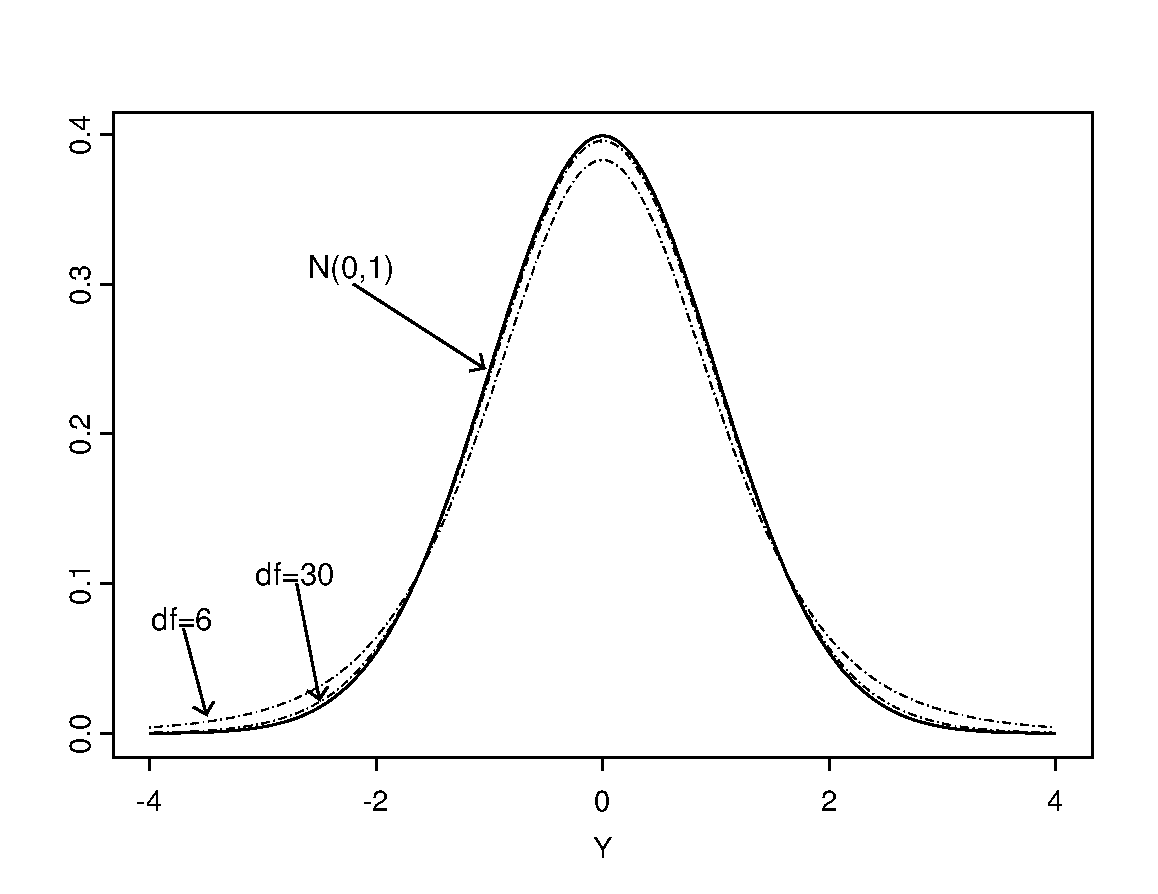
\includegraphics[width=13.00000cm]{tdistr1.pdf}
\caption{\label{fig:f-tdistr1} Curves of two \(t\) distributions with small
degrees of freedom, compared to the standard normal distribution.}
\end{figure}

If we use this result for the test, the \(P\)-value is obtained from the
\(t\) distribution with \(n_{1}+n_{2}-2\) degrees of freedom (often
denoted \(t_{n1+n2-2}\)). The principles of doing this are exactly the
same as those described in Section \ref{ss-probs-test1sample-samplingd},
and can be graphically illustrated by plots similar to those in Figure
\ref{fig:f-pval-prob}. Precise \(P\)-values are again obtained using a
computer. In fact, \(P\)-values in SPSS output for the two-sample
\(t\)-test (c.f.~Figure \ref{fig:f-spss2test}) are actually those
obtained from the \(t\) distribution (with the degrees of freedom shown
in the column labelled ``df'') rather than the standard normal
distribution. Differences between the two are, however, very small if
the sample sizes are even moderately large, because then the degrees of
freedom \(df=n_{1}+n_{2}-2\) are large enough for the two distributions
to be virtually identical. This is the case, for instance, in both of
the examples considered so far in this chapter, where \(df=1102\) in
Example 7.2 and \(df=131\) in Example 7.3.

If precise \(P\)-values from the \(t\) distribution are not available,
upper bounds for them can again be obtained using appropriate tables, in
the same way as in Section \ref{ss-probs-test1sample-samplingd}. Now,
however, the critical values depend also on the degrees of freedom.
Because of this, introductory text books on statistics typically include
a table of critical values for \(t\) distributions for a selection of
degrees of freedom. A table of this kind is shown at the beginning of
Section \ref{s-disttables-t} at the end of this course pack. Each row of
the table corresponds to a \(t\) distribution with the degrees of
freedom given in the column labelled ``df''. As here, such tables
typically include all degrees of freedom between 1 and 30, plus a
selection of larger values, here 40, 60 and 120.

The last row is labelled ``\(\infty\)'', the mathematical symbol for
infinity. This corresponds to the standard normal distribution, as a
\(t\) distribution with infinite degrees of freedom is equal to the
standard normal. The practical implication of this is that the standard
normal distribution is a good enough approximation for any \(t\)
distribution with reasonably large degrees of freedom. The table thus
lists individual degrees of freedom only up to some point, and the last
row will be used for any values larger than this. For degrees of freedom
between two values shown in the table (e.g.~50 when only 40 and 60 are
given), it is best to use the values for the nearest available degrees
of freedom \emph{below} the required ones (e.g.~use 40 for 50). This
will give a ``conservative'' approximate \(P\)-value which may be
slightly larger than the exact value.

As for the standard normal distribution, the table is used to identify
critical values for different significance levels (c.f.~the information
in Table \ref{tab:t-ttable}). For example, if the degrees of freedom are
20, the critical value for two-sided tests at the significance level
0.05 in the ``0.025'' column on the row labelled ``20''. This is 2.086.
In general, critical values for \(t\) distributions are somewhat larger
than corresponding values for the standard normal distribution, but the
difference between the two is quite small when the degrees of freedom
are reasonably large.

The \(t\)-test and the \(t\) distribution are among the oldest tools of
statistical inference. They were introduced in 1908 by W.~S.
Gosset\footnote{United Nations Development Programme \emph{International
  Human Development Indicators}, \texttt{http://hdr.undp.org/en/data/};
  World Bank \emph{Worldwide Governance Indicators},
  \texttt{http://info.worldbank.org/governance/wgi/pdf/wgidataset.xlsx};
  World Bank \emph{World Development Indicators},
  \texttt{http://data.worldbank.org/indicator/SP.DYN.IMRT.IN}.},
initially for the one-sample case discussed in Section
\ref{s-means-1sample}. Gosset was working as a chemist at the Guinness
brewery at St.~James' Gate, Dublin. He published his findings under the
pseudonym ``Student'', and the distribution is often known as
\emph{Student's \(t\) distribution}.

These results for the sampling distribution hold when the population
standard deviations \(\sigma_{1}\) and \(\sigma_{2}\) are assumed to be
equal. If this assumption is not made, the test statistic is again
calculated using formulas (\ref{eq:seDmu-ne}) and (\ref{eq:ztestmuD}).
This case is mathematically more difficult than the previous one,
because the sampling distribution of the test statistic under the null
hypothesis is then not exactly a \(t\) distribution even when the
population distributions are normal. One way of dealing with this
complication (which is known as the Behrens--Fisher problem) is to find
a \(t\) distribution which is a good approximation of the true sampling
distribution. The degrees of freedom of this approximating distribution
are given by

\begin{equation}df=\frac{\left(
\frac{s^{2}_{1}}{n_{1}}+
\frac{s^{2}_{2}}{n_{2}}
\right)^{2}}
{
\left(\frac{s_{1}^{2}}{n_{1}}\right)^{2}\;
\left(\frac{1}{n_{1}-1}\right)
+
\left(\frac{s_{2}^{2}}{n_{2}}\right)^{2}\;
\left(\frac{1}{n_{2}-1}\right)
}.
\label{eq:satter-df}\end{equation}

This formula, which is known as the Welch-Satterthwaite approximation,
is not particularly interesting or worth learning in itself. It is
presented here purely for completeness, and to give an idea of how the
degrees of freedom given in the SPSS output are obtained. In Example 7.2
(see Figure \ref{fig:f-spss2test}) these degrees of freedom are 945.777,
showing that the approximate degrees of freedom from
(\ref{eq:satter-df}) are often not whole numbers. If approximate
\(P\)-values are then obtained from a \(t\)-table, we need to use values
for the nearest whole-number degrees of freedom shown in the table. This
problem does not arise if the calculations are done with a computer.

Two sample \(t\)-test statistics (in two variants, under equal and
unequal population standard deviations) have now been defined under two
different sets of assumptions about the population distributions. In
each case, the formula of the test statistic is the same, so the only
difference is in the form of its sampling distribution under the null
hypothesis. If the population distributions of \(Y\) in the two groups
are assumed to be normal, the sampling distribution of the
\(t\)-statistic is a \(t\) distribution with appropriate degrees of
freedom. If the sample sizes are reasonably large, the sampling
distribution is approximately standard normal, whatever the shape of the
population distribution. Which set of assumptions should we then use?
The following guidelines can be used to make the choice:

\begin{itemize}
\item
  The easiest and arguably most common case is the one where both sample
  sizes \(n_{1}\) and \(n_{2}\) are large enough (both greater than 20,
  say) for the standard normal approximation of the sampling
  distribution to be reasonably accurate. Because the degrees of freedom
  of the appropriate \(t\) distribution are then also large, the two
  sampling distributions are very similar, and conclusions from the test
  will be similar in either case. It is then purely a matter of
  convenience which sampling distribution is used:

  \begin{itemize}
  \item
    If you use a computer (e.g.~SPSS) to carry out the test or you are
    (e.g.~in an exam) given computer output, use the \(P\)-value in the
    output. This will be from the \(t\) distribution.
  \item
    If you need to calculate the test statistic by hand and thus need to
    use tables of critical values to draw the conclusion, use the
    critical values for the standard normal distribution (see Table
    \ref{tab:t-ttable}).
  \end{itemize}
\item
  When the sample sizes are small (e.g.~if one or both of them are less
  than 20), only the \(t\) distribution can be used, and even then only
  if \(Y\) is approximately normally distributed in both groups in the
  population. For some variables (say weight or blood pressure) we might
  have some confidence that this is the case, perhaps from previous,
  larger studies. In other cases the normality of \(Y\) can only be
  assessed based on its sample distribution, which of course is not very
  informative when the sample is small. In most cases, some doubt will
  remain, so the results of a \(t\)-test from small samples should be
  treated with caution. An alternative is then to use
  \emph{nonparametric} tests which avoid the assumption of normality,
  for example the so-called Wilcoxon--Mann--Whitney test. These,
  however, are not covered on this course.
\end{itemize}

There are also situations where the population distribution of \(Y\)
cannot possibly be normal, so the possibility of referring to a \(t\)
distribution does not arise. One example are the tests on population
proportions that were discussed in Chapter \ref{c-probs}. There the only
possibility we discussed was to use the approximate standard normal
sampling distribution, as long as the sample sizes were large enough.
Because the \(t\)-distribution is never relevant there, the test
statistic is conventionally called the \(z\)-test statistic rather than
\(t\). Sometimes the label \(z\) instead of \(t\) is used also for
two-sample \(t\)-statistics described in this chapter. This does not
change the test itself.

It is also possible to obtain a confidence interval for \(\Delta\) which
is valid for even very small sample sizes \(n_{1}\) and \(n_{2}\), but
only under the further assumption that the population distribution of
\(Y\) in both groups is normal. This affects only the multiplier of the
standard errors, which is now based on a \(t\) distribution. The
appropriate degrees of freedom are again \(df=n_{1}+n_{2}-2\) when the
population standard deviations are assumed equal, and approximately
given by equation (\ref{eq:satter-df}) if not. In this case the
multiplier in (\ref{eq:ciDpa}) may be labelled \(t^{(df)}_{\alpha/2}\)
instead of \(z_{\alpha/2}\) to draw attention to the fact that it comes
from a \(t\)-distribution and depends on the degrees of freedom \(df\)
as well as the significance level \(1-\alpha\).

Any multiplier \(t_{\alpha/2}^{(df)}\) is obtained from the relevant
\(t\) distribution using exactly the same logic as the one explained for
the normal distribution in the previous section, using a computer or a
table of \(t\) distributions. For example, in the \(t\) table at the
beginning of Section \ref{s-disttables-t}, multipliers for a 95\%
confidence interval are the numbers given in the column labelled
``0.025''. Suppose, for instance, that the sample sizes \(n_{1}\) and
\(n_{2}\) are both 10 and population standard deviations are assumed
equal, so that \(df=10+10-2=18\). The table shows that a \(t\)-based
95\% confidence interval would then use the multiplier 2.101. This is
somewhat larger than the corresponding multiplier 1.96 from the normal
distribution, and the \(t\)-based interval is somewhat wider than one
based on the normal distribution. The difference between the two becomes
very small when the sample sizes are even moderately large, because then
\(df\) is large and \(t_{\alpha/2}^{(df)}\) is very close to 1.96.

The choice between confidence intervals based on the normal or a \(t\)
distribution involves the same considerations as for the significance
test. In short, if the sample sizes are not very small, the choice makes
little difference and can be based on convenience. If you are
calculating an interval by hand, a normal-based one is easier to use
because the multiplier (e.g.~1.96 for 95\% intervals) does not depend on
the sample sizes. If, instead, a computer is used, it typically gives
confidence intervals for differences of means based on the \(t\)
distribution, so these are easier to use. Finally, if one or both of the
sample sizes are small, only \(t\)-based intervals can safely be used,
and then only if you are confident that the population distributions of
\(Y\) are approximately normal.

\section{Tests and confidence intervals for a single
mean}\label{s-means-1sample}

The task considered in this section is inference on the population mean
of a continuous, interval-level variable \(Y\) in a single population.
This is thus analogous to the analysis of a single proportion in
Sections \ref{s-probs-test1sample}--\ref{s-probs-1sampleci}, but with a
continuous variable of interest.

We use Example 7.1 on survey data on diet for illustration. We will
consider two variables, daily consumption of portions of fruit and
vegetables, and the percentage of total faily energy intake obtained
from fat and fatty acids. These will be analysed separately, each in
turn in the role of the variable of interest \(Y\). Summary statistics
for the variables are shown in Table \ref{tab:t-ttests1}

\begin{longtable}[]{@{}lrrrrrrrc@{}}
\caption{\label{tab:t-ttests1} Summary statistics, \(t\)-tests and
confidence intervals for the mean for the two variables in Example 7.1
(variables from the Diet and Nutrition Survey). \(n=\)sample size;
\(\bar{Y}=\)sample mean; \(s=\)sample standard deviation;
\(\mu_{0}=\)null hypothesis about the population mean; \(t=t\)-test
statistic; \(*\): Alternative hypothesis \(H_{a}: \mu\ne \mu_{0}\);
\(\dagger\): Alternative hypotheses \(H_{a}: \mu<5\) and \(\mu>35\)
respectively.}\tabularnewline
\toprule
\begin{minipage}[t]{0.30\columnwidth}\raggedright\strut
\strut
\end{minipage} & \begin{minipage}[t]{0.04\columnwidth}\raggedleft\strut
\strut
\end{minipage} & \begin{minipage}[t]{0.05\columnwidth}\raggedleft\strut
\strut
\end{minipage} & \begin{minipage}[t]{0.03\columnwidth}\raggedleft\strut
\strut
\end{minipage} & \begin{minipage}[t]{0.05\columnwidth}\raggedleft\strut
\strut
\end{minipage} & \begin{minipage}[t]{0.03\columnwidth}\raggedleft\strut
\strut
\end{minipage} & \begin{minipage}[t]{0.13\columnwidth}\raggedleft\strut
\(P\)-value\strut
\end{minipage} & \begin{minipage}[t]{0.08\columnwidth}\raggedleft\strut
\(P\)-value\strut
\end{minipage} & \begin{minipage}[t]{0.06\columnwidth}\centering\strut
\strut
\end{minipage}\tabularnewline
\begin{minipage}[t]{0.30\columnwidth}\raggedright\strut
Variable\strut
\end{minipage} & \begin{minipage}[t]{0.04\columnwidth}\raggedleft\strut
\(n\)\strut
\end{minipage} & \begin{minipage}[t]{0.05\columnwidth}\raggedleft\strut
\(\bar{Y}\)\strut
\end{minipage} & \begin{minipage}[t]{0.03\columnwidth}\raggedleft\strut
\(s\)\strut
\end{minipage} & \begin{minipage}[t]{0.05\columnwidth}\raggedleft\strut
\(\mu_{0}\)\strut
\end{minipage} & \begin{minipage}[t]{0.03\columnwidth}\raggedleft\strut
\(t\)\strut
\end{minipage} & \begin{minipage}[t]{0.13\columnwidth}\raggedleft\strut
Two- sided\(^{*}\)\strut
\end{minipage} & \begin{minipage}[t]{0.08\columnwidth}\raggedleft\strut
One- sided\(^{\dagger}\)\strut
\end{minipage} & \begin{minipage}[t]{0.06\columnwidth}\centering\strut
95\% CI for \(\mu\)\strut
\end{minipage}\tabularnewline
\begin{minipage}[t]{0.30\columnwidth}\raggedright\strut
Fruit and vegetable consumption (400g portions)\strut
\end{minipage} & \begin{minipage}[t]{0.04\columnwidth}\raggedleft\strut
1724\strut
\end{minipage} & \begin{minipage}[t]{0.05\columnwidth}\raggedleft\strut
2.8\strut
\end{minipage} & \begin{minipage}[t]{0.03\columnwidth}\raggedleft\strut
2.15\strut
\end{minipage} & \begin{minipage}[t]{0.05\columnwidth}\raggedleft\strut
5\strut
\end{minipage} & \begin{minipage}[t]{0.03\columnwidth}\raggedleft\strut
-49.49\strut
\end{minipage} & \begin{minipage}[t]{0.13\columnwidth}\raggedleft\strut
\(<0.001\)\strut
\end{minipage} & \begin{minipage}[t]{0.08\columnwidth}\raggedleft\strut
\(<0.001\)\strut
\end{minipage} & \begin{minipage}[t]{0.06\columnwidth}\centering\strut
(2.70; 2.90)\strut
\end{minipage}\tabularnewline
\begin{minipage}[t]{0.30\columnwidth}\raggedright\strut
Total energy intake from fat (\%)\strut
\end{minipage} & \begin{minipage}[t]{0.04\columnwidth}\raggedleft\strut
1724\strut
\end{minipage} & \begin{minipage}[t]{0.05\columnwidth}\raggedleft\strut
35.3\strut
\end{minipage} & \begin{minipage}[t]{0.03\columnwidth}\raggedleft\strut
6.11\strut
\end{minipage} & \begin{minipage}[t]{0.05\columnwidth}\raggedleft\strut
35\strut
\end{minipage} & \begin{minipage}[t]{0.03\columnwidth}\raggedleft\strut
2.04\strut
\end{minipage} & \begin{minipage}[t]{0.13\columnwidth}\raggedleft\strut
0.042\strut
\end{minipage} & \begin{minipage}[t]{0.08\columnwidth}\raggedleft\strut
0.021\strut
\end{minipage} & \begin{minipage}[t]{0.06\columnwidth}\centering\strut
(35.01; 35.59)\strut
\end{minipage}\tabularnewline
\bottomrule
\end{longtable}

The setting for the analysis of this section is summarised as a
statistical model for observations of a variable \(Y\) as follows:

\begin{enumerate}
\def\labelenumi{\arabic{enumi}.}
\item
  The population distribution of \(Y\) has some unknown mean \(\mu\) and
  unknown standard deviation \(\sigma\).
\item
  The observations \(Y_{1}, Y_{2}, \dots, Y_{n}\) in the sample are a
  random sample from the population.
\item
  The observations are statistically independent, as discussed at the
  beginning of Section \ref{ss-means-inference-intro}.
\end{enumerate}

It is not necessary to assume that the population distribution has a
particular form. However, this is again sometimes assumed to be a normal
distribution, in which case the analyses may be modified in ways
discussed below.

The only quantity of interest considered here is \(\mu\), the population
mean of \(Y\). In the diet examples this is the mean number of portions
of fruit and vegetables, or mean percentage of energy derived from fat
(both on an average day for an individual) among the members of the
population (which for this survey is British adults aged 19--64).

Because no separate groups are being compared, questions of interest are
now not about differences between different group means, but about the
value of \(\mu\) itself. The best single estimate (\emph{point
estimate}) of \(\mu\) is the sample mean \(\bar{Y}\). More information
is provided by a confidence interval which shows which values of \(\mu\)
are plausible given the observed data.

Significance testing focuses on the question of whether it is plausible
that the true value of \(\mu\) is equal to a particular value
\(\mu_{0}\) specified by the researcher. The specific value of
\(\mu_{0}\) to be tested is suggested by the research questions. For
example, we will consider \(\mu_{0}=5\) for portions of fruit and
vegetables and \(\mu_{0}=35\) for the percentage of energy from fat.
These values are chosen because they correspond to recommendations by
the Department of Health that we should consume at least 5 portions of
fruit and vegetables a day, and that fat should contribute no more than
35\% of total energy intake. The statistical question is thus whether
the average level of consumption in the population is at the recommended
level.

In this setting, the null hypothesis for a significance test will be of
the form

\begin{equation}H_{0}: \; \mu=\mu_{0},
\label{eq:H01}\end{equation}

i.e.~it claims that the unknown population mean \(\mu\) is equal to the
value \(\mu_{0}\) specified by the null hypothesis. This will be tested
against the two-sided alternative hypothesis

\begin{equation}H_{a}: \; \mu\ne \mu_{0}
\label{eq:Ha1two}\end{equation}

or one of the one-sided alternative hypotheses

\begin{equation}H_{a}:  \mu> \mu_{0} \label{eq:Ha1onegt}\end{equation}

or

\begin{equation}H_{a}:  \mu< \mu_{0}.\label{eq:Ha1onelt}\end{equation}

For example, we might consider the one-sided alternative hypotheses
\(H_{a}:\; \mu<5\) for portions of fruit and vegetables and
\(H_{a}:\;\mu>35\) for the percentage of energy from fat. For both of
these, the alternative corresponds to a difference from \(\mu_{0}\) in
the unhealthy direction, i.e.~less fruit and vegetables and more fat
than are recommended.

To establish a connection to the general formulas that have been stated
previously, it is again useful to express these hypotheses in terms of

\begin{equation}\Delta=\mu-\mu_{0},\label{eq:D1mu}\end{equation}

i.e.~the difference between the unknown true mean \(\mu\) and the value
\(\mu_{0}\) claimed by the null hypothesis. Because this is 0 if and
only if \(\mu\) and \(\mu_{0}\) are equal, the null hypothesis
(\ref{eq:H01}) can also be expressed as

\begin{equation}H_{0}: \; \Delta=0,\label{eq:H0D}\end{equation}

and possible alternative hypotheses as

\begin{equation}H_{0}: \Delta\ne0, \label{eq:HaDtwo}\end{equation}

\begin{equation}H_{0}: \Delta>0 \label{eq:HaDonegt}\end{equation}

and

\begin{equation}H_{0}:  \Delta< 0,   \label{eq:HaDonelt}\end{equation}

corresponding to (\ref{eq:Ha1two}), (\ref{eq:Ha1onegt}) and
(\ref{eq:Ha1onelt}) respectively.

The general formulas summarised in Section
\ref{ss-means-inference-intro} can again be used, as long as their
details are modified to apply to \(\Delta\) defined as \(\mu-\mu_{0}\).
The resulting formulas are listed briefly below, and then illustrated
using the data from the diet survey:

\begin{itemize}
\item
  The point estimate of the difference \(\Delta=\mu-\mu_{0}\) is

  \begin{equation}\hat{\Delta}=\bar{Y}-\mu_{0}.
  \label{eq:Dhat1}\end{equation}
\item
  The standard error of \(\hat{\Delta}\), i.e.~the standard deviation of
  its sampling distribution, is
  \(\sigma_{\hat{\Delta}}=\sigma/\sqrt{n}\) (note that this is equal to
  the standard error \(\sigma_{\bar{Y}}\) of the sample mean \(\bar{Y}\)
  itself\footnote{ESS Round 5: European Social Survey Round 5 Data
    (2010). Data file edition 2.0. Norwegian Social Science Data
    Services, Norway � Data Archive and distributor of ESS data. The
    full data can be obtained from
    \texttt{http://ess.nsd.uib.no/ess/round5/}.}). This is estimated by

  \begin{equation}\hat{\sigma}_{\hat{\Delta}} = \frac{s}{\sqrt{n}}.
  \label{eq:seDhat1}\end{equation}
\item
  The \(t\)-test statistic for testing the null hypothesis
  (\ref{eq:H0D}) is

  \begin{equation}t=\frac{\hat{\Delta}}{\hat{\sigma}_{\hat{\Delta}}} =
  \frac{\bar{Y}-\mu_{0}}{s/\sqrt{n}}.
  \label{eq:tD1}\end{equation}
\item
  The sampling distribution of the \(t\)-statistic, when the null
  hypothesis is true, is approximately a standard normal distribution,
  when the sample size \(n\) is reasonably large. A common rule of thumb
  is that this sampling distribution is adequate when \(n\) is at least
  30.

  \begin{itemize}
  \tightlist
  \item
    Alternatively, we may make the further assumption that the
    population distribution of \(Y\) is normal, in which case no
    conditions on \(n\) are required. The sampling distribution of \(t\)
    is then a \(t\) distribution with \(n-1\) degrees of freedom. The
    choice of which sampling distribution to refer to is based on the
    considerations outlined in Section
    \ref{ss-means-inference-variants}. When \(n\) is 30 or larger, the
    two approaches give very similar results.
  \end{itemize}
\item
  \(P\)-values are obtained and the conclusions drawn in the same way as
  for two-sample tests, with appropriate modifications to the wording of
  the conclusions.
\item
  A confidence interval for \(\Delta\), with confidence level
  \(1-\alpha\) and based on the approximate normal sampling
  distribution, is given by

  \begin{equation}\hat{\Delta}\pm z_{\alpha/2}\, \hat{\sigma}_{\hat{\Delta}}
  =
  (\bar{Y}-\mu_{0}) \pm z_{\alpha/2} \, \frac{s}{\sqrt{n}}
  \label{eq:ciD1}\end{equation}

  where \(z_{\alpha/2}\) is the multiplier from the standard normal
  distribution for the required significance level (see Table
  \ref{tab:t-ciq}), most often 1.96 for a 95\% confidence interval. If
  an interval based on the \(t\) distribution is wanted instead,
  \(z_{\alpha/2}\) is replaced by the corresponding multiplier
  \(t_{\alpha/2}^{(n-1)}\) from the \(t_{n-1}\) distribution.

  Instead of the interval (\ref{eq:ciD1}) for the difference
  \(\Delta=\mu-\mu_{0}\), it is usually more sensible to report a
  confidence interval for \(\mu\) itself. This is given by

  \begin{equation}\bar{Y} \pm z_{\alpha/2} \, \frac{s}{\sqrt{n}},
  \label{eq:cimu1}\end{equation}

  which is obtained by adding \(\mu_{0}\) to both end points of
  (\ref{eq:ciD1}).
\end{itemize}

For the fruit and vegetable variable in the diet example, the mean under
the null hypothesis is the dietary recommendation \(\mu_{0}=5\). The
estimated difference (\ref{eq:Dhat1}) is \[\hat{\Delta}=2.8-5=-2.2\] and
its estimated standard error (\ref{eq:seDhat1}) is
\[\hat{\sigma}_{\hat{\Delta}}= \frac{2.15}{\sqrt{1724}} = 0.05178,\] so
the \(t\)-test statistic (\ref{eq:tD1}) is
\[t=\frac{-2.2}{0.05178} = -42.49.\] To obtain the \(P\)-value for the
test, \(t=-42.49\) is referred to the sampling distribution under the
null hypothesis, which can here be taken to be the standard normal
distribution, as the sample size \(n=1723\) is large. If we consider the
two-sided alternative hypothesis \(H_{a}:\; \Delta\ne 0\)
(i.e.~\(H_{a}:\; \mu\ne5\)), the \(P\)-value is the probability that a
randomly selected value from the standard normal distribution is at most
\(-42.49\) or at least 42.49. This is a very small probability,
approximately \(0.00\cdots019\), with 268 zeroes between the decimal
point and the 1. This is, of course, to all practical purposes zero, and
can be reported as \(P<0.001\). The null hypothesis \(H_{0}:\; \mu=5\)
is rejected at any conventional level of significance. A \(t\)-test for
the mean indicates very strong evidence that the average daily number of
portions of fruit and vegetables consumed by members of the population
differs from the recommended minimum of five.

If we considered instead the one-sided alternative hypothesis
\(H_{a}:\;\Delta<0\) (i.e.~\(H_{a}: \; \mu<5\)), the observed sample
mean \(\bar{Y}=2.8<5\) is in the direction of this alternative. The
\(P\)-value is then the one-sided \(P\)-value divided by 2, which is
here a small value reported as \(P<0.001\) again. The null hypothesis
\(H_{0}: \; \mu=5\) (and by implication also the one-sided null
hypothesis \(H_{0}:\; \mu\ge 5\), as discussed at the end of Section
\ref{ss-probs-test1sample-hypotheses}) is thus also rejected in favour
of this one-sided alternative, at any conventional significance level.

A 95\% confidence interval for \(\mu\) is obtained from (\ref{eq:cimu1})
as \[2.8\pm 1.96 \times \frac{2.15}{\sqrt{1724}}
=2.8\pm 1.96 \times 0.05178=
2.8\pm 0.10 = (2.70; 2.90).\] We are thus 95\% confident that the
average daily number of portions of fruit and vegetables consumed by
members of the population is between 2.70 and 2.90.

Figure \ref{fig:f-spsstest} shows how these results for the fruit and
vegetable variable are displayed in SPSS output. The label ``portions''
refers to the name given to the variable in the SPSS data file, and
``Test Value = 5'' indicates the null hypothesis value \(\mu_{0}\) being
tested. \label{p-ttest-expl}Other parts of the SPSS output correspond to
the information in Table \ref{tab:t-ttests1} in fairly obvious ways, so
``N'' indicates the sample size \(n\) (and not a population size, which
is denoted by \(N\) in our notation), ``Mean'' the sample mean
\(\bar{Y}\), ``Std.~Deviation'' the sample standard deviation \(s\),
``Std.~Error Mean'' the estimate of the standard error of the mean given
by \(s/\sqrt{n}=2.15/\sqrt{1724}=0.05178\), ``Mean Difference'' the
difference \(\hat{\Delta}=\bar{Y}-\mu_{0}=2.8-5=-2.2\), and ``t'' the
\(t\)-test statistic (\ref{eq:tD1}). The \(P\)-value against the
two-sided alternative hypothesis is shown as ``Sig.~(2-tailed)''
(reported in the somewhat sloppy SPSS manner as ``.000''). This is
actually obtained from the \(t\) distribution, the degrees of freedom of
which (\(n-1=1723\)) are given under ``df''. Finally, the output also
contains a 95\% confidence interval for the difference
\(\Delta=\mu-\mu_{0}\), i.e.~the interval (\ref{eq:ciD1}).\footnote{This
  is another old idea. Different approaches to the problem of fitting
  curves to observations were gradually developed by Tobias Mayer,
  Rudjer Bošković and Pierre Simon Laplace from the 1750s onwards, and
  the method of least squares itself was presented by Adrien Marie
  Legendre in 1805.} This is given as \((-2.30; -2.10)\). To obtain the
more convenient confidence interval (\ref{eq:cimu1}) for \(\mu\) itself,
we only need to add \(\mu_{0}=5\) to both end points of the interval
shown by SPSS, to obtain \((-2.30+5; -2.10+5)=(2.70; 2.90)\) as before.

\begin{figure}[htbp]
\centering
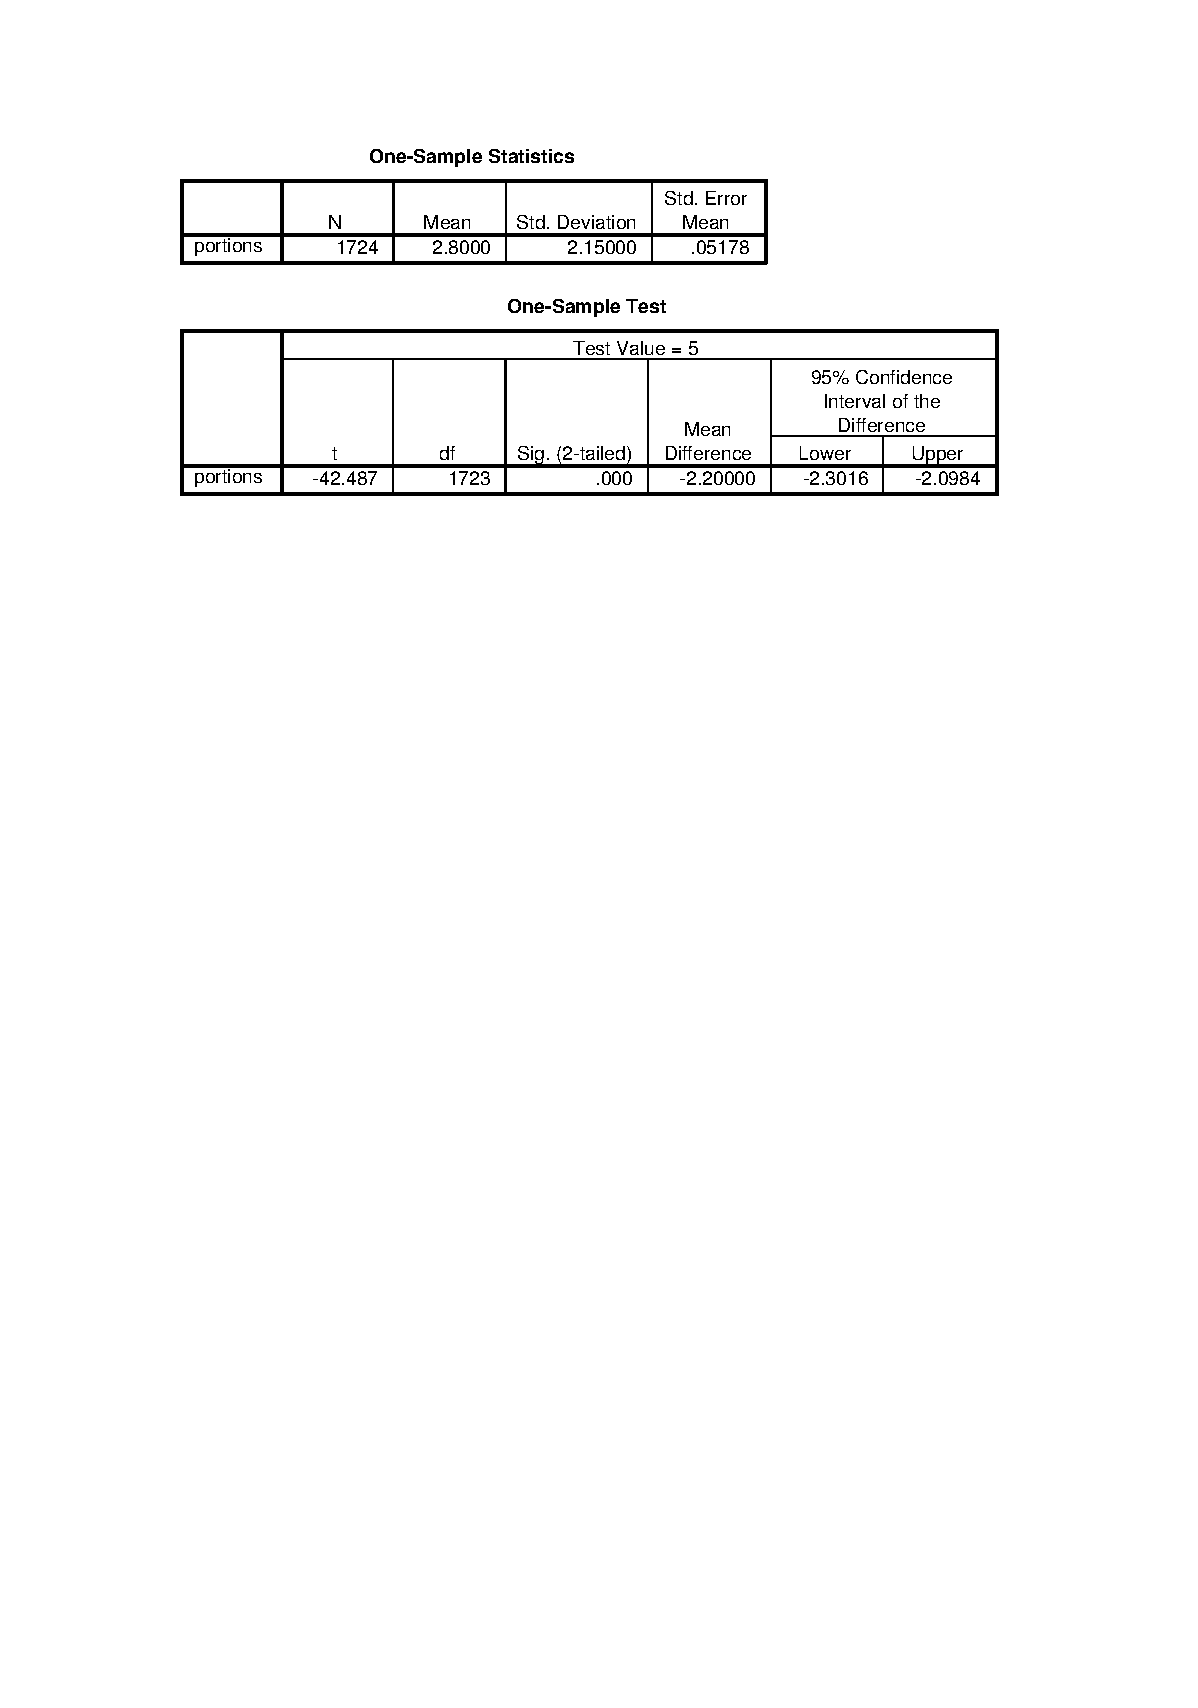
\includegraphics[width=13.00000cm]{ttestspss.pdf}
\caption{\label{fig:f-spsstest} SPSS output for a \(t\)-test of a single
mean. The output is for the variable on fruit and vegetable consumption
in Table \ref{tab:t-ttests1}, with the null hypothesis
\(H-{0}: \mu=5\).}
\end{figure}

Similar results for the variable on the percentage of dietary energy
obtained from fat are also shown in Table \ref{tab:t-ttests1}. Here
\(\mu_{0}=35\), \(\hat{\Delta}=35.3-35=0.3\),
\(\hat{\sigma}_{\hat{\Delta}}=6.11/\sqrt{1724}=0.147\), \(t=0.3/0.147\),
and the two-sided \(P\)-value is \(P=0.042\). Here \(P<0.05\), so null
hypothesis that the population average of the percentage of energy
obtained from fat is 35 is rejected at the 5\% level of significance.
However, because \(P>0.01\), the hypothesis would not be rejected at the
next conventional significance level of 1\%. The conclusions are the
same if we considered the one-sided alternative hypothesis
\(H_{a}:\; \mu>35\), for which \(P=0.042/2=0.021\) (as the observed
sample mean \(\bar{Y}=35.3\) is in the direction of \(H_{a}\)). In this
case the evidence against the null hypothesis is thus somewhat less
strong than for the fruit and vegetable variable, for which the
\(P\)-value was extremely small. The 95\% confidence interval for the
population average of the fat variable is
\(35.3\pm 1.96\times 0.147=(35.01; 35.59)\).

Analysis of a single population mean is a good illustration of some of
the advantages of confidence intervals over significance tests. First, a
confidence interval provides a summary of all the plausible values of
\(\mu\) even when, as is very often the case, there is no obvious single
value \(\mu_{0}\) to be considered as the null hypothesis of the
one-sample \(t\)-test. Second, even when such a significance test is
sensible, the conclusion can also be obtained from the confidence
interval, as discussed at the end of Section \ref{ss-means-ci-vstests}.
In other words, \(H_{0}:\; \mu=\mu_{0}\) is rejected at a given
significance level against a two-sided alternative hypothesis, if the
confidence interval for \(\mu\) at the corresponding confidence level
does not contain \(\mu_{0}\), and not rejected if the interval contains
\(\mu_{0}\). Here the 95\% confidence interval (2.70; 2.90) does not
contain 5 for the fruit and vegetable variable, and the interval (35.01;
35.59) does not contain 35 for the fat variable, so the null hypotheses
with these values as \(\mu_{0}\) are rejected at the 5\% level of
significance.

The width of a confidence interval also gives information on how precise
the results of the statistical analysis are. Here the intervals seem
quite narrow for both variables, in that it seems that their end points
(e.g.~2.7 and 2.9 for portions of fruit and vegetables) would imply
qualitatively similar conclusions about the level of consumption in the
population. Analysis of the sample of 1724 respondents in the National
Diet and Nutrition Survey thus appears to have given us quite precise
information on the population averages for most practical purposes. Of
course, what is precise enough ultimately depends on what those purposes
are. If much higher precision was required, the sample size in the
survey would have to be correspondingly larger.

Finally, in cases where a null hypothesis is rejected by a significance
test, a confidence interval has the additional advantage of providing a
way to assess whether the observed deviation from the null hypothesis
seems large in some \emph{substantive} sense. For example, the
confidence interval for the fat variable draws attention to the fact
that the evidence against a population mean of 35 is not very strong.
The lower bound of the interval is only 0.01 units above 35, which is
very little relative to the overall width (about 0.60) of the interval.
The \(P\)-value (0.041) of the test, which is not much below the
reference level of 0.05, also suggests this, but in a less obvious way.
Even the upper limit (35.59) of the interval is arguably not very far
from 35, so it suggests that we can be fairly confident that the
population mean does not differ from 35 by very much in the substantive
sense. This contrasts with the results for the fruit and vegetable
variable, where all the values covered by the confidence interval (2.70;
2.90) are much more obviously far from the recommended value of 5.

\section{Inference for dependent samples}\label{s-means-dependent}

In the two-sample cases considered in Section \ref{s-means-inference},
the two groups being compared consisted of separate and presumably
unrelated units (people, in all of these cases). It thus seemed
justified to treat the groups as statistically independent. The third
and last general case considered in this chapter is one where this
assumption cannot be made, because there are some obvious connections
between the groups. \protect\hyperlink{p-dependentex}{Examples 7.4 and
7.5} illustrate this situation. Specifically, in both cases we can find
for each observation in one group a natural \emph{pair} in the other
group. In Example 7.4, the data consist of observations of a variable
for a group of fathers at two time points, so the pairs of observations
are clearly formed by the two measurements for each father. In Example
7.5 the basic observations are for separate days, but these are paired
(\emph{matched}) in that for each Friday the 13th in one group, the
preceding Friday the 6th is included in the other. In both cases the
existence of the pairings implies that we must treat the two groups as
statistically \emph{dependent}.

Data with dependent samples are quite common, largely because they are
often very informative. Principles of good research design suggest that
one key condition for being able to make valid and powerful comparisons
between two groups is that the groups should be as similar as possible,
apart from differing in the characteristic being considered. Dependent
samples represent an attempt to achieve this through intelligent data
collection. In Example 7.4, the comparison of interest is between a
man's sense of well-being before and after the birth of his first child.
It is likely that there are also other factors which affect well-being,
such as personality and life circumstances unrelated to the birth of a
child. Here, however, we can compare the well-being for the \emph{same}
men before and after the birth, which should mean that many of those
other characteristics remain approximately unchanged between the two
measurements. Information on the effects of the birth of a child will
then mostly come not from overall levels of well-being but
\emph{changes} in it for each man.

In Example 7.5, time of the year and day of the week are likely to have
a very strong effect on traffic levels. Comparing, say, Friday, November
13th to Friday, July 6th, let alone to Sunday, November 15th, would thus
not provide much information about possible additional differences which
were due specifically to a Friday being the 13th. To keep these other
characteristics approximately constant and thus to focus on the effects
of Friday the 13th, each such Friday has here been matched with the
nearest preceding Friday. With this design, data on just ten matched
pairs will (as seen below) allow us to conclude that the differences are
statistically significant.

Generalisations of the research designs illustrated by Examples 7.4 and
7.5 allow for measurements at more than two occasions for each subject
(so-called longitudinal or panel studies) and groups of more than two
matched units (clustered designs). Most of these are analysed using
statistical methods which are beyond the scope of this course. The
paired case is an exception, for which the analysis is in fact easier
than for two independent samples. This is because the pairing of
observations allows us to reduce the analysis into a one-sample problem,
simply by considering within-pair \emph{differences} in the response
variable \(Y\). Only the case where \(Y\) is a continuous variable is
considered here. There are also methods of inference for comparing two
(or more) dependent samples of response variables of other types, but
they are not covered here.

The quantity of interest is again a population difference. This time it
can be formulated as \(\Delta=\mu_{2}-\mu_{1}\), where \(\mu_{1}\) is
the mean of \(Y\) for the first group (e.g.~the first time point in
Example 7.4) and \(\mu_{2}\) its mean for the second group. Methods of
inference for \(\Delta\) will again be obtained using the same general
results which were previously applied to one-sample analyses and
comparisons of two independent samples. The easiest way to do this is
now to consider a new variable \(D\), defined for each \emph{pair} \(i\)
as \(D_{i}=Y_{2i}-Y_{1i}\), where \(Y_{1i}\) denotes the value of the
first measurement of \(Y\) for pair \(i\), and \(Y_{2i}\) is the second
measurement of \(Y\) for the same pair. In Example 7.4 this is thus the
difference between a man's well-being after the birth of his first baby,
and the same man's well-being before the birth. In Example 7.5, \(D\) is
the difference in traffic flows on a stretch of motorway between a
Friday the 13th and the Friday a week earlier (these values are shown in
the last column of Table \ref{tab:t-F13}). The number of observations of
\(D\) is the number of pairs, which is equal to the sample sizes
\(n_{1}\) and \(n_{2}\) in each of the two groups (the case where one of
the two measurements might be missing for some pairs is not considered
here). We will denote it by \(n\).

The population mean of the differences \(D\) is also
\(\Delta=\mu_{2}-\mu_{1}\), so the observed values \(D_{i}\) can be used
for inference on \(\Delta\). An estimate of \(\Delta\) is the sample
average of \(D_{i}\), i.e.

\begin{equation}\hat{\Delta}=\overline{D}=\frac{1}{n}\sum_{i=1}^{n} D_{i}.
\label{eq:Dbar-dep}\end{equation}

In other words, this is the average of the within-pair differences
between the two measurements of \(Y\). Its standard error is estimated
by

\begin{equation}\hat{\sigma}_{\hat{\Delta}} =
\frac{s_{D}}{\sqrt{n}}
\label{eq:sDbar-dep}\end{equation}

where \(s_{D}\) is the sample standard deviation of \(D\), i.e.

\begin{equation}s_{D} = \sqrt{\frac{\sum (D_{i}-\overline{D})^{2}}{n-1}}.
\label{eq:s2D-dep}\end{equation}

A test statistic for the null hypothesis \(H_{0}: \Delta=0\) is given by

\begin{equation}t=
\frac{\hat{\Delta}}{\hat{\sigma}_{\hat{\Delta}}}=
\frac{\overline{D}}{s_{D}/\sqrt{n}}
\label{eq:zD-dep}\end{equation}

and its \(P\)-value is obtained either from the standard normal
distribution or the \(t_{n-1}\) distribution. A confidence interval for
\(\Delta\) with confidence level \(1-\alpha\) is given by

\begin{equation}\hat{\Delta} \pm q_{\alpha/2} \times \hat{\sigma}_{\hat{\Delta}}
=\overline{D} \pm q_{\alpha/2} \times \frac{s_{D}}{\sqrt{n}}
\label{eq:ciD-dep}\end{equation}

where the multiplier \(q_{\alpha/2}\) is either \(z_{\alpha/2}\) or
\(t_{\alpha/2}^{(n-1)}\). These formulas are obtained by noting that
this is simply a one-sample analysis with the differences \(D\) in place
of the variable \(Y\), and applying the formulas of Section
\ref{s-means-1sample} to the observed values of \(D\).

\begin{longtable}[]{@{}rrrrr@{}}
\caption{\label{tab:t-2tests-dep} Results of tests and confidence intervals
for comparing means of two dependent samples. For Example 7.4, the
difference is between after and before the birth of the child, and for
Example 7.5 it is between Friday the 13th and the preceding Friday the
6th. See the text for the definitions of the statistics. (* Obtained
from the \(t_{9}\) distribution; \(\dagger\) Obtained from the standard
normal distribution.)}\tabularnewline
\toprule
\begin{minipage}[b]{0.29\columnwidth}\raggedleft\strut
\\strut
\end{minipage} & \begin{minipage}[b]{0.13\columnwidth}\raggedleft\strut
\\strut
\end{minipage} & \begin{minipage}[b]{0.18\columnwidth}\raggedleft\strut
Test of \(H_{0}: \Delta=0\)\strut
\end{minipage} & \begin{minipage}[b]{0.13\columnwidth}\raggedleft\strut
Test of \(H_{0}: \Delta=0\)\strut
\end{minipage} & \begin{minipage}[b]{0.12\columnwidth}\raggedleft\strut
\\strut
\end{minipage}\tabularnewline
\midrule
\endfirsthead
\toprule
\begin{minipage}[b]{0.29\columnwidth}\raggedleft\strut
\\strut
\end{minipage} & \begin{minipage}[b]{0.13\columnwidth}\raggedleft\strut
\\strut
\end{minipage} & \begin{minipage}[b]{0.18\columnwidth}\raggedleft\strut
Test of \(H_{0}: \Delta=0\)\strut
\end{minipage} & \begin{minipage}[b]{0.13\columnwidth}\raggedleft\strut
Test of \(H_{0}: \Delta=0\)\strut
\end{minipage} & \begin{minipage}[b]{0.12\columnwidth}\raggedleft\strut
\\strut
\end{minipage}\tabularnewline
\midrule
\endhead
\begin{minipage}[t]{0.29\columnwidth}\raggedleft\strut
\(\hat{\Delta}\)\strut
\end{minipage} & \begin{minipage}[t]{0.13\columnwidth}\raggedleft\strut
\(\hat{\sigma}_{\hat{\Delta}}\)\strut
\end{minipage} & \begin{minipage}[t]{0.18\columnwidth}\raggedleft\strut
\(t\)\strut
\end{minipage} & \begin{minipage}[t]{0.13\columnwidth}\raggedleft\strut
\(P\)-value\strut
\end{minipage} & \begin{minipage}[t]{0.12\columnwidth}\raggedleft\strut
95 \% C.I. for \(\Delta\)\strut
\end{minipage}\tabularnewline
\begin{minipage}[t]{0.29\columnwidth}\raggedleft\strut
Example 7.4: Father's personal well-being\strut
\end{minipage} & \begin{minipage}[t]{0.13\columnwidth}\raggedleft\strut
\strut
\end{minipage} & \begin{minipage}[t]{0.18\columnwidth}\raggedleft\strut
\strut
\end{minipage} & \begin{minipage}[t]{0.13\columnwidth}\raggedleft\strut
\strut
\end{minipage} & \begin{minipage}[t]{0.12\columnwidth}\raggedleft\strut
\strut
\end{minipage}\tabularnewline
\begin{minipage}[t]{0.29\columnwidth}\raggedleft\strut
0.08\strut
\end{minipage} & \begin{minipage}[t]{0.13\columnwidth}\raggedleft\strut
0.247\strut
\end{minipage} & \begin{minipage}[t]{0.18\columnwidth}\raggedleft\strut
0.324\strut
\end{minipage} & \begin{minipage}[t]{0.13\columnwidth}\raggedleft\strut
0.75\(^{\dagger}\)\strut
\end{minipage} & \begin{minipage}[t]{0.12\columnwidth}\raggedleft\strut
(-0.40; 0.56)\strut
\end{minipage}\tabularnewline
\begin{minipage}[t]{0.29\columnwidth}\raggedleft\strut
Example 7.5: Traffic flows on successive Friday\strut
\end{minipage} & \begin{minipage}[t]{0.13\columnwidth}\raggedleft\strut
\strut
\end{minipage} & \begin{minipage}[t]{0.18\columnwidth}\raggedleft\strut
\strut
\end{minipage} & \begin{minipage}[t]{0.13\columnwidth}\raggedleft\strut
\strut
\end{minipage} & \begin{minipage}[t]{0.12\columnwidth}\raggedleft\strut
\strut
\end{minipage}\tabularnewline
\begin{minipage}[t]{0.29\columnwidth}\raggedleft\strut
-1835\strut
\end{minipage} & \begin{minipage}[t]{0.13\columnwidth}\raggedleft\strut
372\strut
\end{minipage} & \begin{minipage}[t]{0.18\columnwidth}\raggedleft\strut
-4.93\strut
\end{minipage} & \begin{minipage}[t]{0.13\columnwidth}\raggedleft\strut
0.001\(^{*}\)\strut
\end{minipage} & \begin{minipage}[t]{0.12\columnwidth}\raggedleft\strut
(-2676; -994)\strut
\end{minipage}\tabularnewline
\bottomrule
\end{longtable}

Results for Examples 7.4 and 7.5 are shown in Table
\ref{tab:t-2tests-dep}. To illustrate the calculations, consider Example
7.5. The \(n=10\) values of \(D_{i}\) for it are shown in Table
\ref{tab:t-F13}, and the summary statistics \(\overline{D}=-1835\) and
\(s_{D}=1176\) in Table \ref{tab:t-groupex}. The standard error of
\(\overline{D}\) is thus \(s_{D}/\sqrt{n}=1176/\sqrt{10}=372\) and the
value of the test statistic (\ref{eq:zD-dep}) is
\[z=\frac{-1835}{1176/\sqrt{10}}=\frac{-1835}{372}=-4.93.\] This example
differs from others we have considered so far in that the sample size of
\(n=10\) is clearly too small for us to rely on large-sample results. It
is thus not appropriate to refer the test statistic to a standard normal
distribution. Instead, \(P\)-values can be obtained from a \(t\)
distribution, but only if the population distribution of \(D\) itself
can be assumed to be approximately normal. Here we have only the ten
observed values of \(D\) to use for a rather informal assessment of
whether this assumption appears to be reasonable. One value of \(D\) is
smaller than -4000, and 2, 5, 2 of them are in the ranges -3000 to
-2001, -2000 to -1001, and -1000 to -1 respectively. Apart from the
smallest observation, the sample distribution of \(D\) is thus at least
approximately symmetric. While this definitely does not prove that \(D\)
is normally distributed, it is at least not obviously inconsistent with
such a claim. We thus feel moderately confident that we can apply here
tests and confidence intervals based on the \(t\) distribution.

The \(P\)-value, obtained from a \(t\) distribution with \(n-1=9\)
degrees of freedom, for the test statistic \(-4.93\) is approximately
0.001. Even with only ten pairs of observations, there is significant
evidence that the volume of traffic on a Friday the 13th differs from
that of the preceding Friday. A confidence interval for the difference
is obtained from (\ref{eq:ciD-dep}) as
\[-1835 \pm 2.26 \times 372 = (-2676; -994)\] where the multiplier 2.26
is the quantity \(t_{\alpha/2}^{(n-1)}=t_{0.975}^{(9)}\), obtained from
a computer or a table of the \(t_{9}\)-distribution. The interval shows
that we are 95\% confident that the average reduction in traffic on
Friday the 13th on the stretches of motorway considered here is between
994 and 2676 vehicles. This seems like a substantial systematic
difference, although not particularly large as a proportion of the total
volume of traffic on those roads. In the absence of other information we
are tempted to associate the reduction with some people avoiding driving
on a day they consider to be unlucky.

In Example 7.4 the \(P\)-value is 0.75, so we cannot reject the null
hypothesis that \(\Delta=0\). There is thus no evidence that there was a
difference in first-time fathers' self-assessed level of well-being
between the time their wives were six months pregnant, and a month after
the birth of the baby. This is also indicated by the 95\% confidence
interval \mbox{($-0.40$; 0.56)} for the difference, which clearly covers
the value 0 of no difference.

\section{Further comments on significance tests}\label{s-means-tests3}

Some further aspects of significance testing are dicussed here. These
are not practical issues that need to be actively considered every time
you carry out a test. Instead, they provide context and motivation for
the principles behind significance tests.

\subsection{Different types of error}\label{ss-means-tests3-errors}

Consider for the moment the approach to significance testing where the
outcome is presented in the form of a discrete claim or decision about
the hypotheses, stating that the null hypothesis was either rejected or
not rejected. This claim can either be correct or incorrect, depending
on whether the null hypothesis is true in the population. There are four
possibilities, summarized in Table \ref{tab:t-twoerrors}. Two of these
are correct decisions and two are incorrect. The two kinds of incorrect
decisions are traditionally called

\begin{itemize}
\item
  \textbf{Type I error:} rejecting the null hypothesis when it is true
\item
  \textbf{Type II error:} not rejecting the null hypothesis when it is
  false
\end{itemize}

The terms are unmemorably bland, but they do at least suggest an order
of importance. Type I error is conventionally considered more serious
than Type II, so what we most want to avoid is rejecting the null
hypothesis unnecessarily. This implies that we will maintain the null
hypothesis unless data provide strong enough evidence to justify
rejecting it, a principle which is somewhat analogous to the ``keep a
theory until falsified'' thinking of Popperian philosophy of science, or
even the ``innocent until proven guilty'' principle of jurisprudence.

\begin{longtable}[]{@{}llll@{}}
\caption{\label{tab:t-twoerrors} The four possible combinations of the truth
of a null hypothesis \(H_{0}\) in a population and decision about it
from a significance test.}\tabularnewline
\toprule
& & \(H_{0}\) & \(H_{0}\)\tabularnewline
& & Not Rejected & Rejected\tabularnewline
\(H_{0}\) is & True & Correct decision & Type I error\tabularnewline
& False & Type II error & Correct decision\tabularnewline
\bottomrule
\end{longtable}

Dispite our dislike of Type I errors, we will not try to avoid them
completely. The only way to guarantee that the null hypothesis is never
incorrectly rejected is never to reject it at all, whatever the
evidence. This is not a useful decision rule for empirical research.
Instead, we will decide in advance how high a probability of Type I
error we are willing to tolerate, and then use a test procedure with
that probability. Suppose that we use a 5\% level of significance to
make decisions from a test. The null hypothesis is then rejected if the
sample yields a test statistic for which the \(P\)-value is less than
0.05. If the null hypothesis is actually true, such values are, by the
definition of the \(P\)-value, obtained with probability 0.05. Thus the
significance level (\(\alpha\)-level) of a test is the probability of
making a Type I error. If we use a large \(\alpha\)-level (say
\(\alpha=0.10\)), the null hypothesis is rejected relatively easily
(whenever \(P\)-value is less than 0.10), but the chances of committing
a Type I error are correspondingly high (also 0.10); with a smaller
value like \(\alpha=0.01\), the error probability is lower because
\(H_{0}\) is rejected only when evidence against it is quite strong.

This description assumes that the true probability of Type I error for a
test \emph{is} equal to its stated \(\alpha\)-level. This is true when
the assumptions of the test (about the population distribution, sample
size etc.) are satisfied. If the assumptions fail, the true significance
level will differ from the stated one, i.e.~the \(P\)-value calculated
from the standard sampling distribution for that particular test will
differ from the true \(P\)-value which would be obtained from the exact
sampling distribution from the population in question. Sometimes the
difference is minor and can be ignored for most practical purposes (the
test is then said to be \emph{robust} to violations of some of its
assumptions). In many situations, however, using an inappropriate test
may lead to incorrect conclusions: for example, a test which claims that
the \(P\)-value is 0.02 when it is really 0.35 will clearly give a
misleading picture of the strength of evidence against the null
hypothesis. To avoid this, the task of statisticians is to develop valid
(and preferably robust) tests for many different kinds of hypotheses and
data. The task of the empirical researcher is to choose a test which is
appropriate for his or her data.

In the spirit of regarding Type I errors as the most serious, the worst
kind of incorrect test is one which gives too low a \(P\)-value,
i.e.~exaggerates the strength of evidence against the null hypothesis.
Sometimes it is known that this is impossible or unlikely, so that the
\(P\)-value is either correct or too high. The significance test is then
said to be \emph{conservative}, because its true rate of Type I errors
will be the same or lower than the stated \(\alpha\)-level. A
conservative procedure of statistical inference is regarded as the next
best thing to one which has the correct level of significance. For
example, when the sample size is relatively large, \(P\)-values for all
of the tests discussed in this chapter may be calculated from a standard
normal or from a \(t\) distribution. \(P\)-values from a \(t\)
distribution are then always somewhat larger. This means that using the
\(t\) distribution is (very slightly) conservative when the population
distributions are not normal, so that we can safely use the \(P\)-values
from SPSS output of a \(t\)-test even in that case (this argument does
not, however, justify using the \(t\)-test when \(Y\) is not normally
distributed and the sample size is small, because the sampling
distribution of the \(t\)-test statistic may then be very far from
normal).

\subsection{Power of significance tests}\label{ss-means-tests3-power}

After addressing the question of Type I error by selecting an
appropriate test and deciding on the significance level to be used, we
turn our attention to Type II errors. The probability that a
significance test will reject the null hypothesis when it is in fact not
true, i.e.~the probability of \emph{avoiding} a Type II error, is known
as the \textbf{power} of the test. It depends, in particular, on

\begin{itemize}
\item
  The nature of the test. If several valid tests are available for a
  particular analysis, we would naturally prefer one which tends to have
  the highest power. One aim of theoretical statistics is to identify
  the most powerful test procedures for different problems.
\item
  The sample size: other things being equal, larger samples mean higher
  power.
\item
  The true value of the population parameter to be tested, here the
  population mean or proportion. The power of any test will be highest
  when the true value is very different from the value specified by the
  null hypothesis. For example, it will obviously be easier to detect
  that a population mean differs from a null value of \(\mu_{0}=5\) when
  the true mean is 25 than when it is 5.1.
\item
  The population variability of the variable. Since large population
  variance translates into large sampling variability and hence high
  levels of uncertainty, the power will be low when population
  variability is large, and high if the population variability is low.
\end{itemize}

The last three of these considerations are often used at the design
stage of a study to get an idea of the sample size required for a
certain level of power, or of the power achievable with a given sample
size. Since data collection costs time and money, we would not want to
collect a much larger sample than is required for a level of certainty
sufficient for the purposes of a study. On the other hand, if a
preliminary calculation reveals that the largest sample we can afford
would still be unlikely to give enough information to detect interesting
effects, the study might be best abandoned.

A power calculation requires the researcher to specify the kinds of
differences from a null hypothesis which are large enough to be of
practical or theoretical interest, so that she or he would want to be
able to detect them with high probability (it must always be accepted
that the power will be lower for smaller differences). For example,
suppose that we are planning a study to compare the effects of two
alternative teaching methods on the performance of students in an
examination where possible scores are between 0 and 100. The null
hypothesis is that average results are the same for students taught with
each method. It is decided that we want enough data to be able to reject
this with high probability if the true difference \(\Delta\) of the
average exam scores between the two groups is larger than 5 points,
i.e.~\(\Delta<-5\) or \(\Delta>5\). The power calculation might then
answer questions like

\begin{itemize}
\item
  What is the smallest sample size for which the probability of
  rejecting \(H_{0}: \Delta=0\) is at least 0.9, when the true value of
  \(\Delta\) is smaller than \(-5\) or larger than 5?
\item
  The largest sample sizes we can afford are 1000 in both groups, i.e.
  \(n_{1}=n_{2}=1000\). What is the probability this gives us of
  rejecting \(H_{0}: \Delta=0\) when the true value of \(\Delta\) is
  smaller than \(-5\) or larger than 5?
\end{itemize}

To answer these questions, we would also need a rough guess of the
population standard deviations \(\sigma_{1}\) and \(\sigma_{2}\),
perhaps obtained from previous studies. Such calculations employ further
mathematical results for test statistics, essentially using their
sampling distributions under specific alternative hypotheses. The
details are, however, beyond the scope of this course.

\subsection{Significance
vs.~importance}\label{ss-means-tests3-importance}

The \(P\)-value is a measure of the strength of evidence the data
provide against the null hypothesis. This is not the same as the
magnitude of the difference between sample estimates and the null
hypothesis, or the practical importance of such differences. As noted
above, the power of a test increases with increasing sampling size. One
implication of this is that when \(n\) is large, even quite small
observed deviations from the values that correspond exactly to the null
hypothesis will be judged to be statistically significant. Consider, for
example, the two dietary variables in Table \ref{tab:t-ttests1}. The
sample mean of the fat variable is 35.3, which is significantly
different (at the 5\% level of significance) from \(\mu_{0}\) of 35. It
is possible, however, that a difference of 0.3 might be considered
unimportant in practice. In contrast, the sample mean of the fruit and
vegetable variable is 2.8, and the difference from \(\mu_{0}\) of 5
seems not only strongly significant but also large for most practical
purposes.

In contrast to the large-sample case, in small samples even quite large
apparent deviations from the null hypothesis might still result in a
large \(P\)-value. For example, in a very small study a sample mean of
the fat variable of, say, 30 or even 50 might not be interpreted as
sufficiently strong evidence against a population mean of 35. This is
obviously related to the discussion of statistical power in the previous
section, in that it illustrates what happens when the sample is too
small to provide enough information for useful conclusions.

In these and all other cases, decisions about what is or is not of
practical importance are subject-matter questions rather than
statistical ones, and would have to be based on information about the
nature and implications of the variables in question. In our dietary
examples this would involve at least medical considerations, and perhaps
also financial implications of the public health costs of the observed
situation or of possible efforts of trying to change it.

\chapter{Linear regression models}\label{c-regression}

\section{Introduction}\label{s-regression-intro}

This chapter continues the theme of analysing statistical associations
between variables. The methods described here are appropriate when the
response variable \(Y\) is a continuous, interval level variable. We
will begin by considering bivariate situations where the only
explanatory variable \(X\) is also a continuous variable. Section
\ref{s-regression-descr} first discusses graphical and numerical
descriptive techniques for this case, focusing on two very commonly used
tools: a \emph{scatterplot} of two variables, and a measure of
association known as the \emph{correlation} coefficient. Section
\ref{s-regression-simple} then describes methods of statistical
inference for associations between two continuous variables. This is
done in the context of a statistical model known as the \emph{simple
linear regression model}.

The ideas of simple linear regression modelling can be extended to a
much more general and powerful set methods known as \emph{multiple
linear regression models}. These can have several explanatory variables,
which makes it possible to examine associations between any explanatory
variable and the response variable, while controlling for other
explanatory variables. An important reason for the usefulness of these
models is that they play a key role in statistical analyses which
correspond to research questions that are causal in nature. As an
interlude, we discuss issues of causality in research design and
analysis briefly in Section \ref{s-regression-causality}. Multiple
linear models are then introduced in Section
\ref{s-regression-multiple}. The models can also include categorical
explanatory variables with any number of categories, as explained in
Section \ref{s-regression-dummies}.

The following example will be used for illustration throughout this
chapter:

\textbf{Example 8.1: Indicators of Global Civil Society}

The \emph{Global Civil Society 2004/5} yearbook gives tables of a range
of characteristics of the countries of the world\footnote{ESS Round 5:
  European Social Survey Round 5 Data (2010). Data file edition 2.0.
  Norwegian Social Science Data Services, Norway � Data Archive and
  distributor of ESS data. The full data can be obtained from
  \texttt{http://ess.nsd.uib.no/ess/round5/}.}. The following measures
will be considered in this chapter:

\begin{itemize}
\item
  Gross Domestic Product (\textbf{GDP}) per capita in 2001 (in current
  international dollars, adjusted for purchasing power parity)
\item
  \textbf{Income level} of the country in three groups used by the
  Yearbook, as Low income, Middle income or High income
\item
  \textbf{Income inequality} measured by the Gini index (with 0
  representing perfect equality and 100 perfect inequality)
\item
  A measure of \textbf{political rights and civil liberties} in 2004,
  obtained as the average of two indices for these characteristics
  produced by the Freedom House organisation (1 to 7, with higher values
  indicating more rights and liberties)
\item
  World Bank Institute's measure of control of \textbf{corruption} for
  2002 (with high values indicating low levels of corruption)
\item
  Net \textbf{primary school enrolment} ratio 2000-01 (\%)
\item
  \textbf{Infant mortality rate} 2001 (\% of live births)
\end{itemize}

We will discuss various associations between these variables. It should
be noted that the analyses are mainly illustrative examples, and the
choices of explanatory and response variables do not imply any strong
claims about causal connections between them. Also, the fact that
different measures refer to slightly different years is ignored; in
effect, we treat each variable as a measure of ``recent'' situation in
the countries. The full data set used here includes 165 countries. Many
of the variables are not available for all of them, so most of the
analyses below use a smaller number of countries.

\section{Describing association between two continuous
variables}\label{s-regression-descr}

\subsection{Introduction}\label{ss-regression-descr-intro}

Suppose for now that we are considering data on two continuous
variables. The descriptive techniques discussed in this section do not
strictly speaking require a distinction between an explanatory variable
and a response variable, but it is nevertheless useful in many if not
most applications. We will reflect this in the notation by denoting the
variables \(X\) (for the explanatory variable) and \(Y\) (for the
response variable). The observed data consist of the pairs of
observations \((X_{1}, Y_{1}), (X_{2}, Y_{2}), \dots, (X_{n}, Y_{n})\)
of \(X\) and \(Y\) for each of the \(n\) subjects in a sample, or, with
more concise notation, \((X_{i}, Y_{i})\) for \(i=1,2,\dots,n\).

We are interested in analysing the association between \(X\) and \(Y\).
Methods for \emph{describing} this association in the sample are first
described in this section, initially with some standard graphical
methods in Section \ref{ss-regression-descr-plots}. This leads to a
discussion in Section \ref{ss-regression-descr-assoc} of what we
actually mean by associations in this context, and then to a definion of
numerical summary measures for such associations in Section
\ref{ss-regression-descr-corr}. Statistical \emph{inference} for the
associations will be considered in Section \ref{s-regression-simple}.

\subsection{Graphical methods}\label{ss-regression-descr-plots}

\subsubsection*{Scatterplots}\label{scatterplots}
\addcontentsline{toc}{subsubsection}{Scatterplots}

The standard statistical graphic for summarising the association between
two continuous variables is a \textbf{scatterplot}. An example of it is
given in Figure \ref{fig:f-corruption1}, which shows a scatterplot of
Control of corruption against GDP per capita for 61 countries for which
the corruption variable is at least 60 (the motivation of this
restriction will be discussed later). The two axes of the plot show
possible values of the two variables. The horizontal axis, here
corresponding to Control of corruption, is conventionally used for the
explanatory variable \(X\), and is often referred to as the
\textbf{X-axis}. The vertical axis, here used for GDP per capita, then
corresponds to the response variable \(Y\), and is known as the
\textbf{Y-axis}.

\begin{figure}[htbp]
\centering
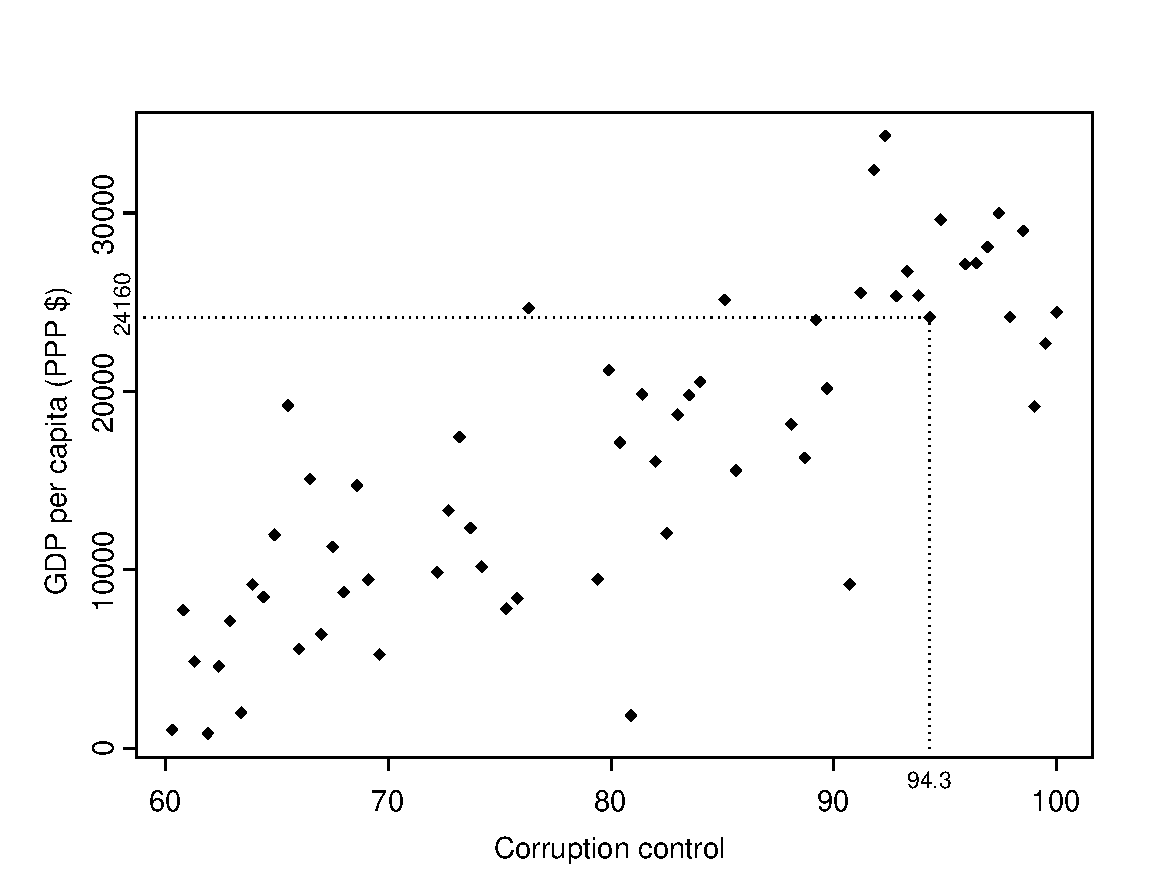
\includegraphics[width=14.00000cm]{corruption1.pdf}
\caption{\label{fig:f-corruption1} A scatterplot of Control of corruption
vs.~GDP per capita in the Global Civil Society data set, for 61
countries with Control of corruption at least 60. The dotted lines are
drawn to the point corresponding to the United Kingdom.}
\end{figure}

The observed data are shown as points in the scatterplot, one for each
of the \(n\) units. The location of each point is determined by its
values of \(X\) and \(Y\). For example, Figure \ref{fig:f-corruption1}
highlights the observation for the United Kingdom, for which the
corruption measure (\(X\)) is 94.3 and GDP per capita (\(Y\)) is
\$24160. The point for UK is thus placed at the intersection of a
vertical line drawn from 94.3 on the \(X\)-axis and a horizontal line
from 24160 on the \(Y\)-axis, as shown in the plot.

The principles of good graphical presentation on clear labelling,
avoidance of spurious decoration and so on (c.f.~Section
\ref{s-descr1-presentation}) are the same for scatterplots as for any
statistical graphics. Because the crucial visual information in a
scatterplot is the shape of the cloud of the points, it is now often not
necessary for the scales of the axes to begin at zero, especially if
this is well outside the ranges of the observed values of the variables
(as it is for the \(X\)-axis of Figure \ref{fig:f-corruption1}).
Instead, the scales are typically selected so that the points cover most
of the plotting surface. This is done by statistical software, but there
are many situations were it is advisable to overrule the automatic
selection (e.g.~for making scatterplots of the same variables in two
different samples directly comparable).

The main purpose of a scatterplot is to examine possible associations
between \(X\) and \(Y\). Loosely speaking, this means considering the
shape and orientation of the cloud of points in the graph. In Figure
\ref{fig:f-corruption1}, for example, it seems that most of the points
are in a cluster sloping from lower left to upper right. This indicates
that countries with low levels of Control of corruption (i.e.~high
levels of corruption itself) tend to have low GDP per capita, and those
with little corruption tend to have high levels of GDP. A more careful
discussion of such associations again relates them to the formal
definition in terms of conditional distributions, and also provides a
basis for the methods of inference introduced later in this chapter. We
will resume the discussion of these issues in Section
\ref{ss-regression-descr-assoc} below. Before that, however, we will
digress briefly from the main thrust of this chapter in order to
describe a slightly different kind of scatterplot.

\subsubsection*{Line plots for time
series}\label{line-plots-for-time-series}
\addcontentsline{toc}{subsubsection}{Line plots for time series}

A very common special case of a scatterplot is one where the
observations correspond to measurements of a variable for the same unit
at several occasions over time. This is illustrated by the following
example (another one is Figure \ref{fig:f-houseprices}):

\emph{Example: Changes in temperature, 1903--2004}

Figure \ref{fig:f-temperatures} summarises data on average annual
temperatures over the past century in five locations. The data were
obtained from the GISS Surface Temperature (GISTEMP) database maintained
by the NASA Goddard Institute for Space Studies\footnote{The data were
  obtained from
  \url{http://data.london.gov.uk/datastore/package/london-borough-profiles}.

  \noindentIf you download the ``Profiles in Excel'' workbook, you will
  find that one of the pages contains a map of the boroughs, and a tool
  for visualising the data on that map. A regular map of the boroughs
  can be found at for example at

  \url{http://www.londoncouncils.gov.uk/londonfacts/londonlocalgovernment/londonmapandlinks/default.htm}.}.
The database contains time series of average monthly surface
temperatures from several hundred meterological stations across the
world. The five sites considered here are Haparanda in Northern Sweden,
Independence, Kansas in the USA, Choshi on the east coast of Japan,
Kimberley in South Africa, and the Base Orcadas Station on Laurie
Island, off the coast of Antarctica. These were chosen rather
haphazardly for this illustration, with the aim of obtaining a
geographically scattered set of rural or small urban locations (to avoid
issues with the heating effects of large urban areas). The temperature
for each year at each location is here recorded as the difference from
the temperature at that location in 1903\footnote{The data can be
  obtained from \texttt{http://www3.norc.org/gss+website/}, which gives
  further information on the survey, including the full text of the
  questionnaires.}.

\begin{figure}[htbp]
\centering
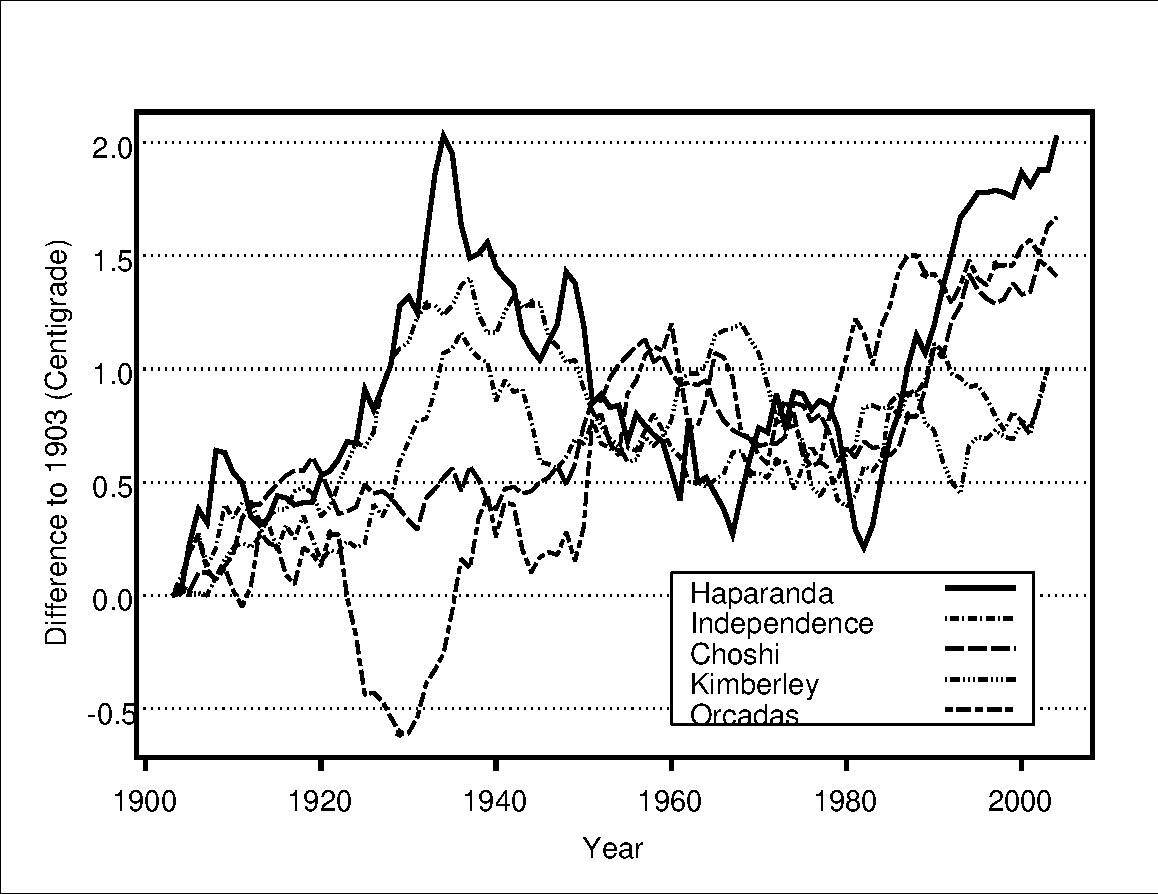
\includegraphics[width=13.00000cm]{temperplot.pdf}
\caption{\label{fig:f-temperatures} Changes of average annual temperature
(11-year moving averages) from 1903 in five locations. See the text for
further details. Source: The GISTEMP database
\textless{}data.giss.nasa.gov/gistemp/\textgreater{}}
\end{figure}

Consider first the data for Haparanda only. Here we have two variables,
year and temperature, and 102 pairs of observations of them, one for
each year between 1903 and 2004. These pairs could now be plotted in a
scatterplot as described above. Here, however, we can go further to
enhance the visual effect of the plot. This is because the observations
represent measurements of a variable (temperature difference) for the
same unit (the town of Haparanda) at several successive times (years).
These 102 measurements form a \emph{time series} of temperature
differences for Haparanda over 1903--2004. A standard graphical trick
for such series is to connect the points for successive times by lines,
making it easy for the eye to follow the changes over time in the
variable on the \(Y\)-axis. In Figure \ref{fig:f-temperatures} this is
done for Haparanda using a solid line. Note that doing this would make
no sense for scatter plots like the one in Figure
\ref{fig:f-corruption1}, because all the points there represent
different subjects, in that case countries.

We can easily include several such series in the same graph. In Figure
\ref{fig:f-temperatures} this is done by plotting the temperature
differences for each of the five locations using different line styles.
The graph now summarises data on three variables, year, temperature and
location. We can then examine changes over time for any one location,
but also compare patterns of changes between them. Here there is clearly
much variation within and between locations, but also some common
features. Most importantly, the temperatures have all increased over the
past century. In all five locations the average annual temperatures at
the end of the period were around 1--2\(^{\circ}\)C higher than in 1903.

A set of time series like this is an example of dependent data in the
sense discussed in Section \ref{s-means-dependent}. There we considered
cases with pairs of observations, where the two observations in each
pair had to be treated as statistically dependent. Here all of the
temperature measurements for one location are dependent, probably with
strongest dependence between adjacent years and less dependence between
ones further apart. This means that we will not be able to analyse these
data with the methods described later in this chapter, because these
assume statistically independent observations. Methods of statistical
modelling and inference for dependent data of the kind illustrated by
the temperature example are beyond the scope of this course. This,
however, does not prevent us from using a plot like Figure
\ref{fig:f-temperatures} to \emph{describe} such data.

\subsection{Linear associations}\label{ss-regression-descr-assoc}

Consider again statistically independent observations of
\((X_{i}, Y_{i})\), such as those displayed in Figure
\ref{fig:f-corruption1}. Recall the definition that two variables are
associated if the conditional distribution of \(Y\) given \(X\) is
different for different values of \(X\). In the two-sample examples of
Chapter \ref{c-means} this could be examined by comparing two
conditional distributions, since \(X\) had only two possible values.
Now, however, \(X\) has many (in principle, infinitely many) possible
values, so we will need to somehow define and compare conditional
distributions given each of them. We will begin with a rather informal
discussion of how this might be done. This will lead directly to a more
precise and formal definition introduced in Section
\ref{s-regression-simple}.

\begin{figure}[htbp]
\centering
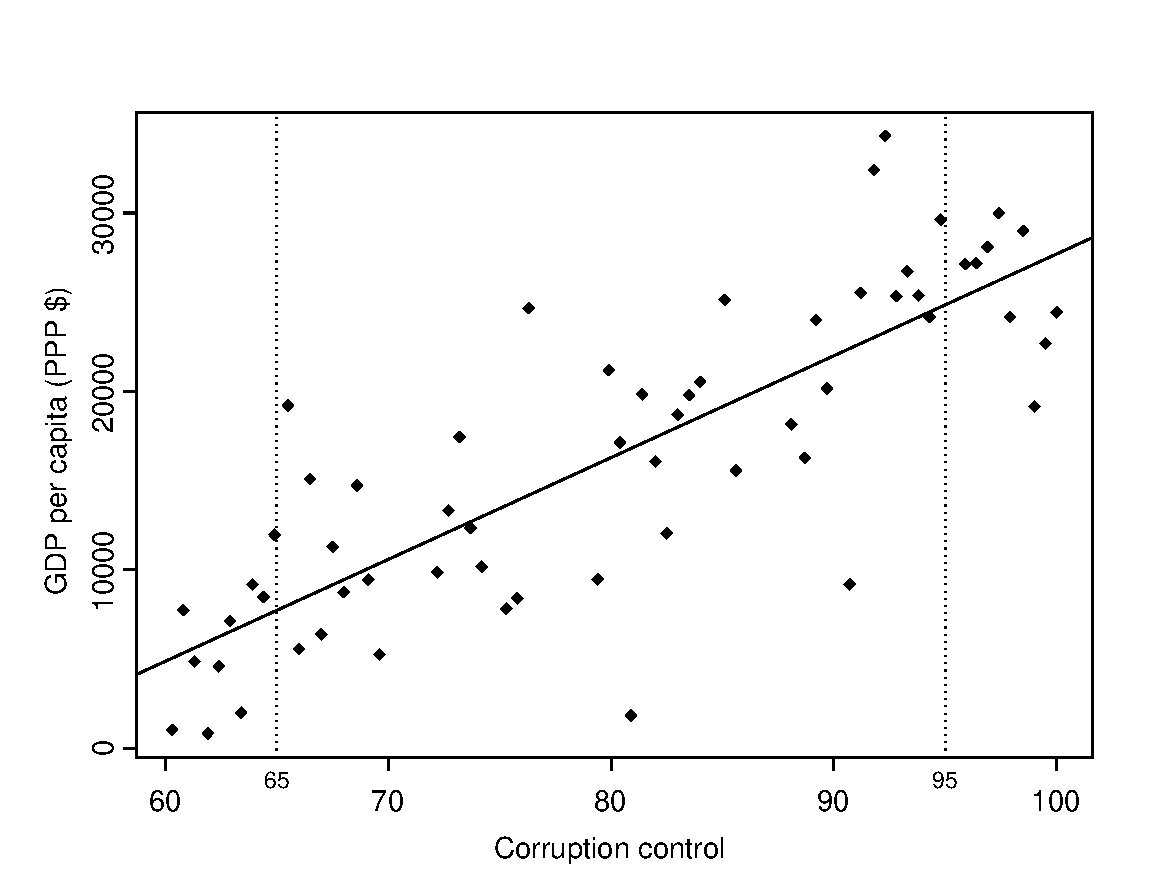
\includegraphics[width=13.50000cm]{corruption2.pdf}
\caption{\label{fig:f-corruption2} The same scatterplot of Control of
corruption vs.~GDP per capita as in Figure \ref{fig:f-corruption1},
augmented by the best-fitting (least squares) straight line (solid line)
and reference lines for two example values of Control of corruption
(dotted lines).}
\end{figure}

Figure \ref{fig:f-corruption2} shows the same scatterplot as Figure
\ref{fig:f-corruption1}. Consider first one value of \(X\) (Control of
corruption), say 65. To get a rough idea of the conditional distribution
of \(Y\) (GDP per capita) given this value of \(X\), we could examine
the sample distribution of the values of \(Y\) for the units for which
the value of \(X\) is close to 65. These correspond to the points near
the vertical line drawn at \(X=65\) in Figure \ref{fig:f-corruption2}.
This can be repeated for any value of \(X\); for example, Figure
\ref{fig:f-corruption2} also includes a vertical reference line at
\(X=95\), for examining the conditional distribution of \(Y\) given
\(X=95\)\footnote{ESS Round 5: European Social Survey Round 5 Data
  (2010). Data file edition 2.0. Norwegian Social Science Data Services,
  Norway � Data Archive and distributor of ESS data. The full data can
  be obtained from \texttt{http://ess.nsd.uib.no/ess/round5/}.}.

As in Chapter \ref{c-means}, associations between variables will here be
considered almost solely in terms of differences in the \emph{means} of
the conditional distributions of \(Y\) at different values of \(X\). For
example, Figure \ref{fig:f-corruption2} suggests that the conditional
mean of \(Y\) when X is 65 is around or just under 10000. At \(X=95\),
on the other hand, the conditional mean seems to be between 20000 and
25000. The mean of \(Y\) is thus higher at the larger value of X. More
generally, this finding is consistent across the scatterplot, in that
the conditional mean of \(Y\) appears to increase when we consider
increasingly large values of \(X\), indicating that higher levels of
Control of corruption are associated with higher average levels of GDP.
This is often expressed by saying that the conditional mean of \(Y\)
increases when we ``increase'' \(X\)\footnote{Strictly speaking, the
  analysis should incorporate sampling weights (variable \emph{DWEIGHT})
  to adjust for different sampling probabilities for different types of
  respondents. Here the weights are ignored. Using them would not change
  the main conclusions for these variables.}. This is the sense in which
we will examine associations between continuous variables: does the
conditional mean of \(Y\) change (increase or decrease) when we increase
\(X\)? If it does, the two variables are associated; if it does not,
there is no association of this kind. This definition also agrees with
the one linking association with prediction: if the mean of \(Y\) is
different for different values of \(X\), knowing the value of \(X\) will
clearly help us in making predictions about likely values of \(Y\).
Based on the information in Figure \ref{fig:f-corruption2}, for example,
our best guesses of the GDPs of two countries would clearly be different
if we were told that the control of corruption measure was 65 for one
country and 95 for the other.

The \emph{nature} of the association between \(X\) and \(Y\) is
characterised by \emph{how} the values of \(Y\) change when \(X\)
increases. First, it is almost always reasonable to conceive these
changes as reasonably smooth and gradual. In other words, if two values
of \(X\) are close to each other, the conditional means of \(Y\) will be
similar too; for example, if the mean of \(Y\) is 5 when \(X=10\), its
mean when \(X=10.01\) is likely to be quite close to 5 rather than, say,
405. In technical terms, this means that the conditional mean of \(Y\)
will be described by a smooth mathematical function of \(X\).
Graphically, the means of \(Y\) as \(X\) increases will then trace a
smooth curve in the scatterplot. The simplest possibility for such a
curve is a straight line. This possibility is illustrated by plot (a) of
Figure \ref{fig:f-scatterplots} (this and the other five plots in the
figure display artificial data, generated for this illustration). Here
all of the points fall on a line, so that when \(X\) increases, the
values of \(Y\) increase at a constant rate. A relationship like this is
known as a \textbf{linear association} between \(X\) and \(Y\). Linear
associations are the starting point for examining associations between
continuous variables, and often the only ones considered. In this
chapter we too will focus almost completely on them.

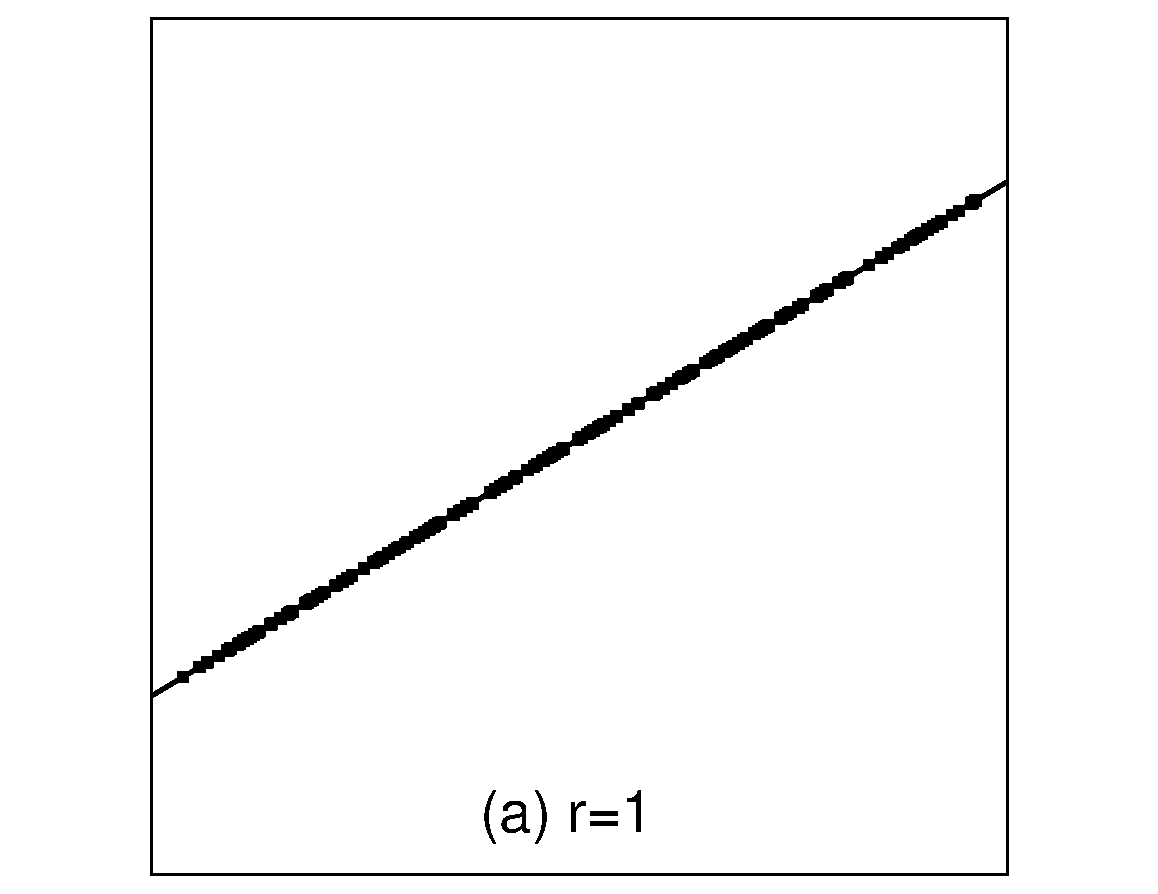
\includegraphics[width=8.00000cm]{olspl1.pdf}
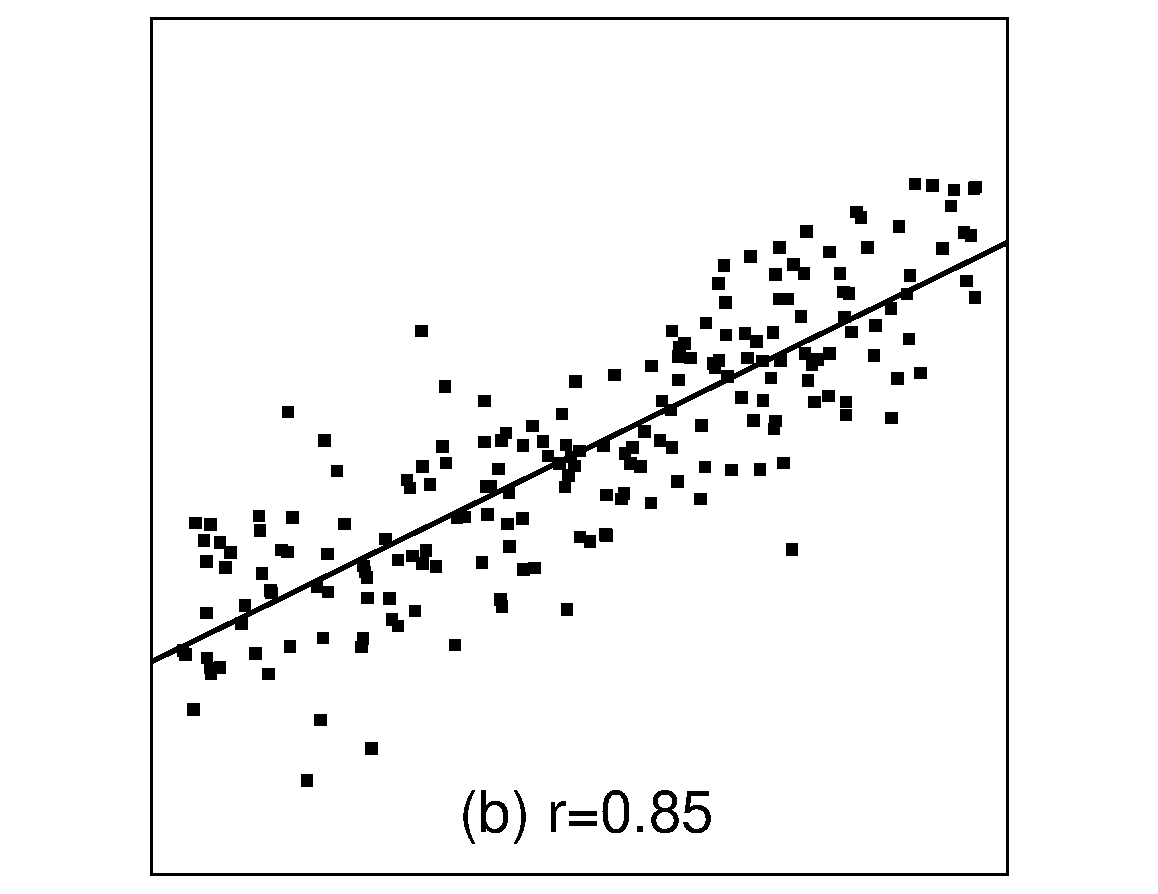
\includegraphics[width=8.00000cm]{olspl2.pdf}\\
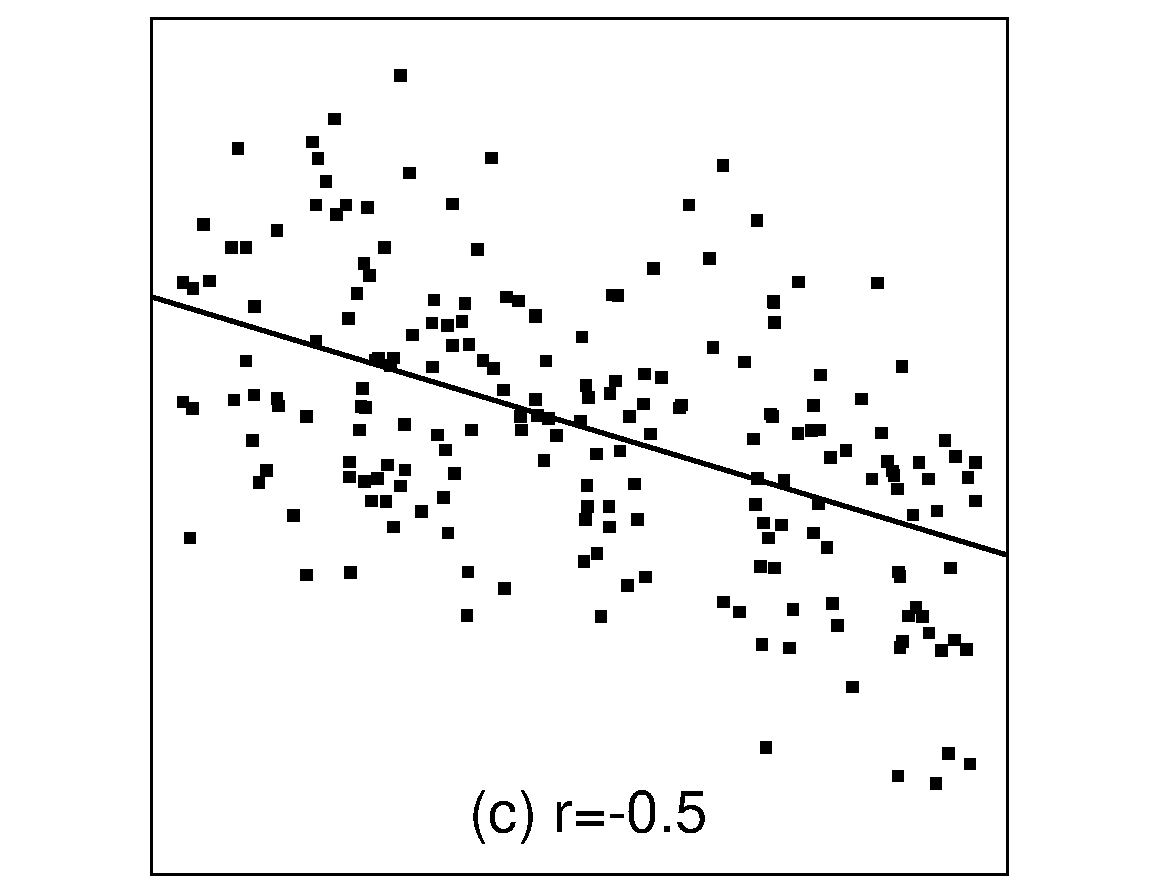
\includegraphics[width=8.00000cm]{olspl3.pdf}
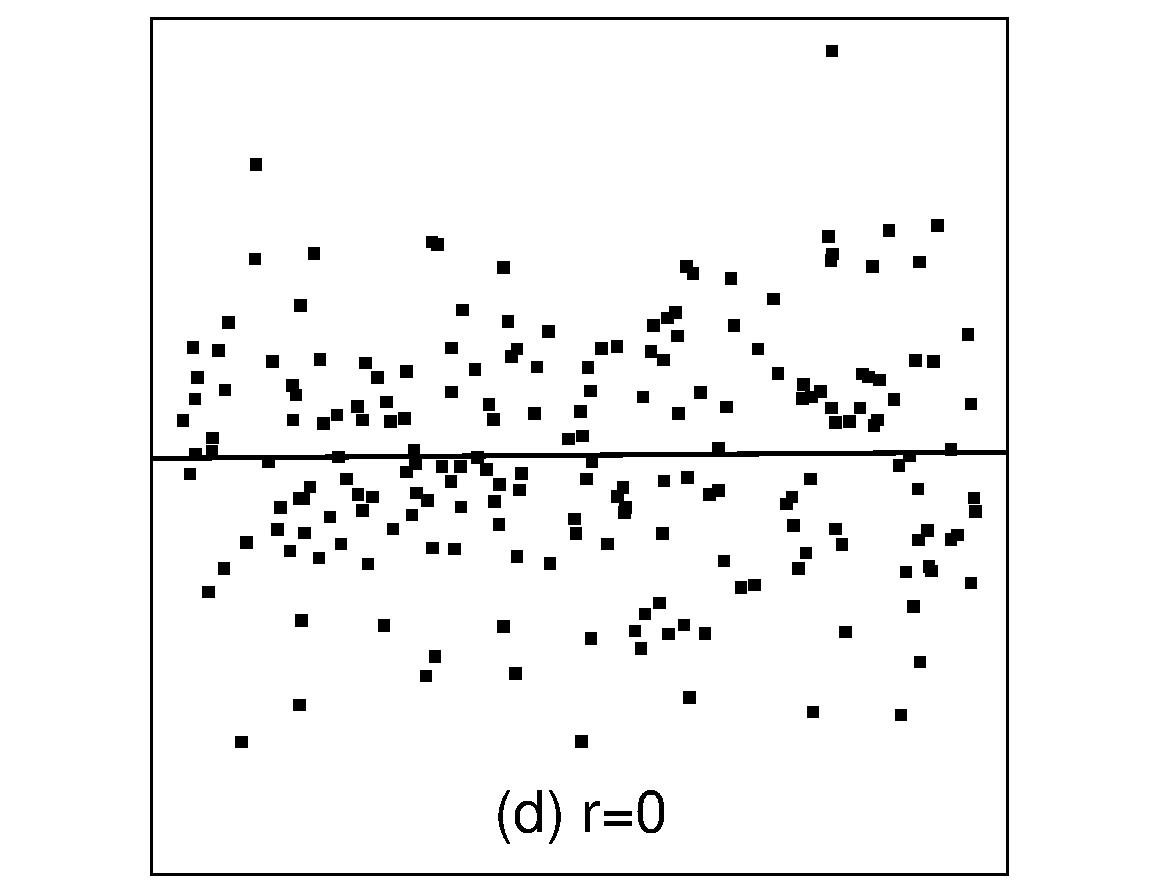
\includegraphics[width=8.00000cm]{olspl4.pdf}\\
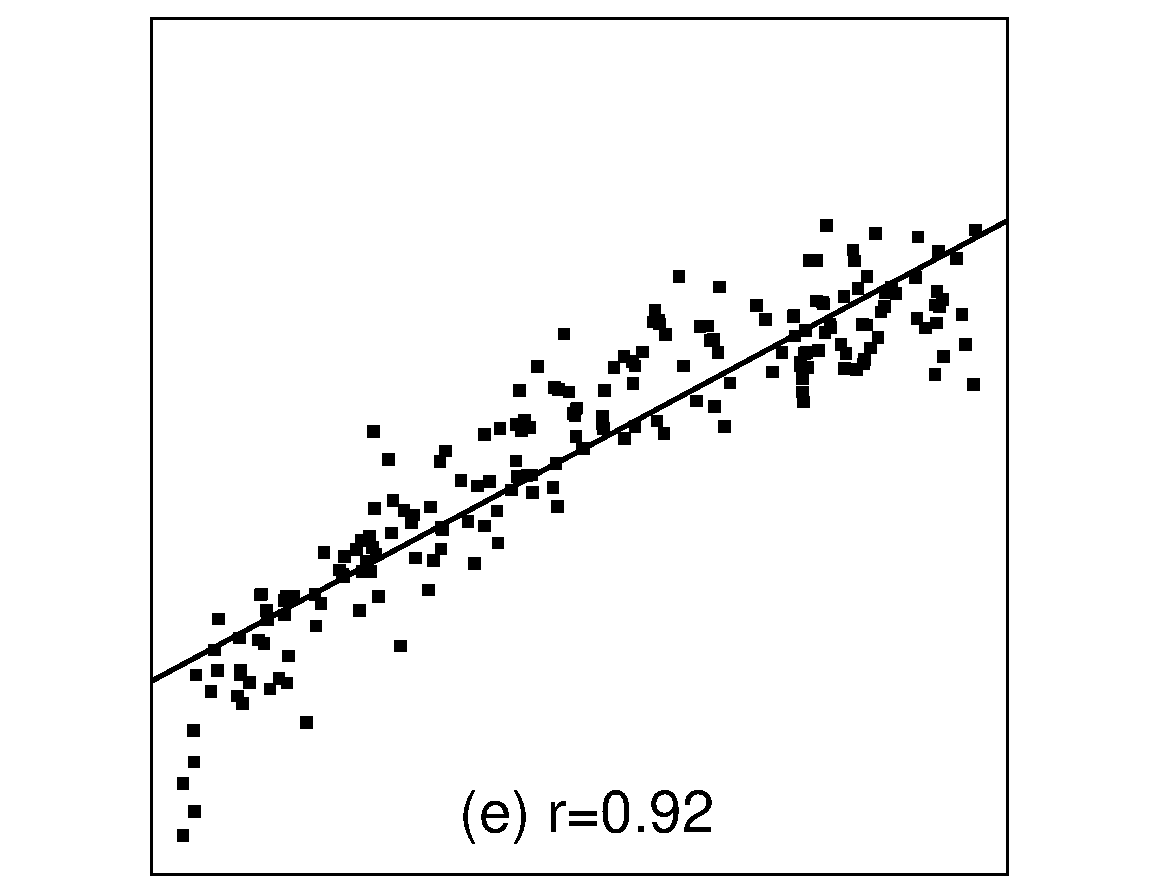
\includegraphics[width=8.00000cm]{olspl5.pdf}
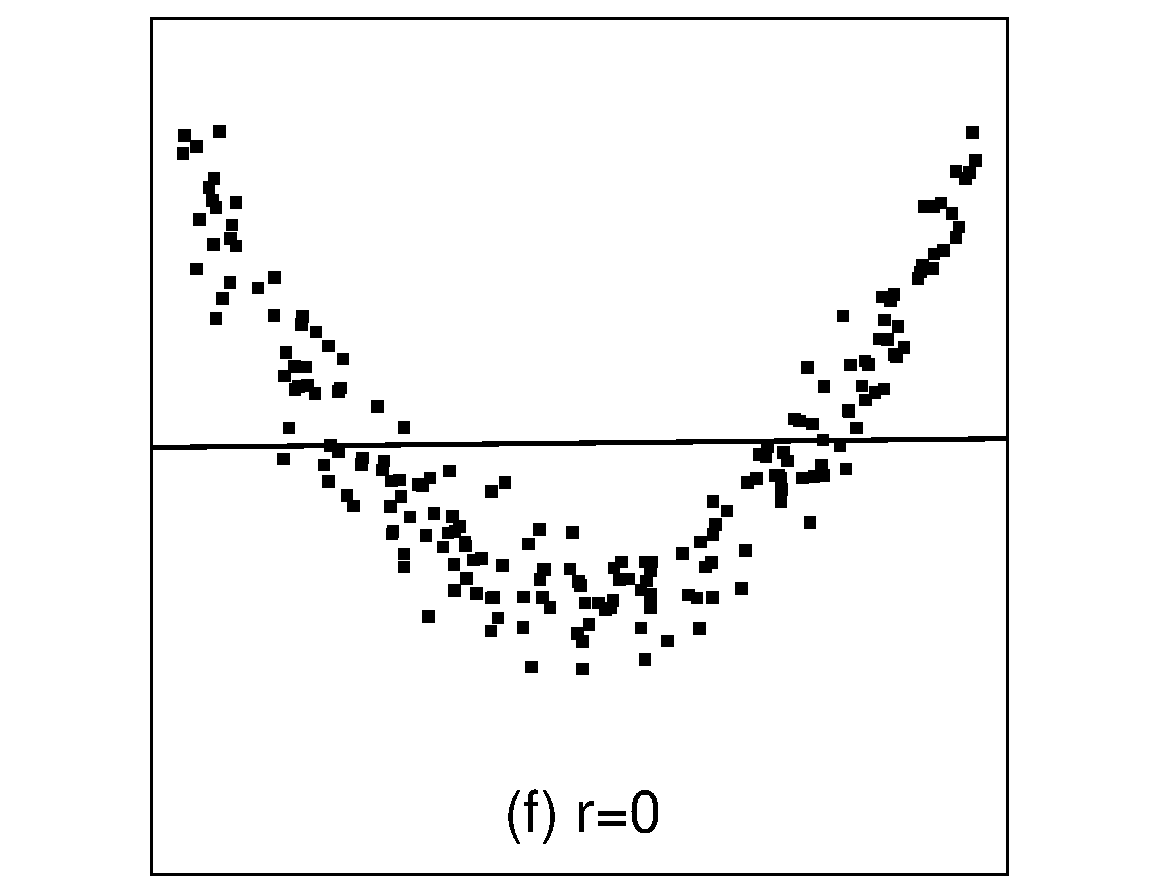
\includegraphics[width=8.00000cm]{olspl6.pdf}\\
In plot (a) of Figure \ref{fig:f-scatterplots} all the points are
exactly on the straight line. This indicates a \emph{perfect} linear
association, where \(Y\) can be predicted exactly if \(X\) is known, so
that the association is \emph{deterministic}. Such a situation is
neither realistic in practice, nor necessary for the association to be
described as linear. All that is required for the latter is that the
conditional \emph{means} of \(Y\) given different values of \(X\) fall
(approximately) on a straight line. This is illustrated by plot (b) of
Figure \ref{fig:f-scatterplots}, which shows a scatterplot of individual
observations together with an approximation of the line of the means of
\(Y\) given \(X\) (how the line was drawn will be explained later). Here
the linear association is not perfect, as the individual points are not
all on the same line but scattered around it. Nevertheless, the line
seems to capture an important systematic feature of the data, which is
that the \emph{average} values of \(Y\) increase at an approximately
constant rate as \(X\) increases. This combination of systematic and
random elements is characteristic of all statistical associations, and
it is also central to the formal setting for statistical inference for
linear associations described in Section \ref{s-regression-simple}
below.

The \textbf{direction} of a linear association can be either
\textbf{positive} or \textbf{negative}. Plots (a) and (b) of Figure
\ref{fig:f-scatterplots} show a positive association, because increasing
\(X\) is associated with increasing average values of \(Y\). This is
indicated by the upward slope of the line describing the association.
Plot (c) shows an example of a negative association, where the line
slopes downwards and increasing values of \(X\) are associated with
decreasing values of \(Y\). The third possibility, illustrated by plot
(d), is that the line slopes neither up nor down, so that the mean of
\(Y\) is the same for all values of \(X\). In this case there is no
(linear) association between the variables.

Not all associations between continuous variables are linear, as shown
by the remaining two plots of Figure \ref{fig:f-scatterplots}. These
illustrate two kinds of \textbf{nonlinear} associations. In plot (e),
the association is still clearly \emph{monotonic}, meaning that average
values of \(Y\) change in the same direction --- here increase --- when
\(X\) increases. The rate of this increase, however, is not constant, as
indicated by the slightly curved shape of the cloud of points. The
values of \(Y\) seem to increase faster for small values of \(X\) than
for large ones. A straight line drawn through the scatterplot captures
the general direction of the increase, but misses its nonlinearity. One
practical example of such a relationship is the one between years of job
experience and salary: it is often found that salary increases fastest
early on in a person's career and more slowly later on.

Plot (f) shows a nonlinear and nonmonotonic relationship: as \(X\)
increases, average values of \(Y\) first decrease to a minimum, and then
increase again, resulting in a U-shaped scatterplot. A straight line is
clearly an entirely inadequate description of such a relationship. A
nonmonotonic association of this kind might be seen, for example, when
considering the dependence of the failure rates of some electrical
components (\(Y\)) on their age (\(X\)). It might then be that the
failure rates were high early (from quick failures of flawed components)
and late on (from inevitable wear and tear) and lowest in between for
``middle-aged but healthy'' components.

\begin{figure}[htbp]
\centering
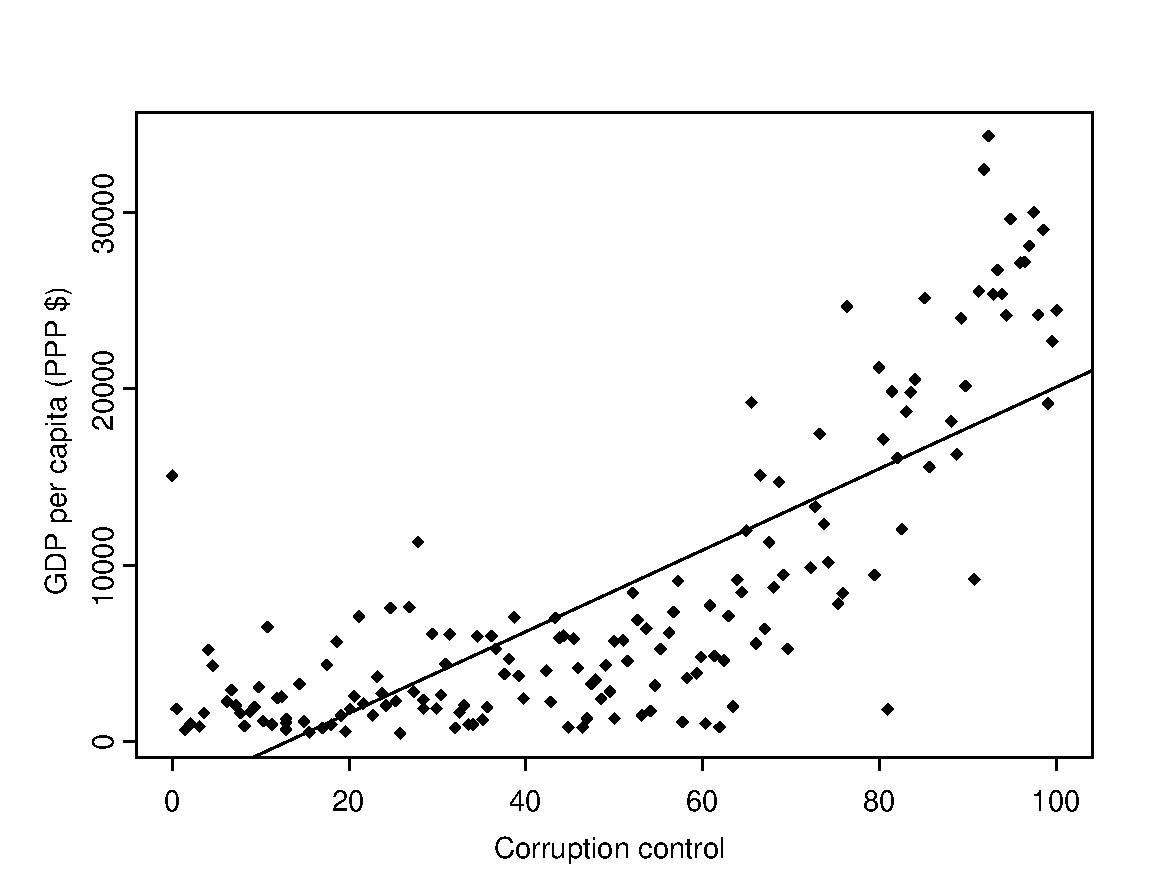
\includegraphics[width=13.50000cm]{corruption3.pdf}
\caption{\label{fig:f-corruption3} A scatterplot of Control of corruption
vs.~GDP per capita for 163 countries in the Global Civil Society data
set. The solid line is the best-fitting (least squares) straight line
for the points.}
\end{figure}

Returning to real data, recall that we have so far considered control of
corruption and GDP per capita only among countries with a Control of
corruption score of at least 60. The scatterplot for these, shown in
Figure \ref{fig:f-corruption2}, also includes a best-fitting straight
line. The observed relationship is clearly positive, and seems to be
fairly well described by a straight line. For countries with relatively
low levels of corruption, the association between control of corruption
and GDP can be reasonably well characterised as linear.

Consider now the set of all countries, including also those with high
levels of corruption (scores of less than 60). In a scatterplot for
them, shown in Figure \ref{fig:f-corruption3}, the points with at least
60 on the \(X\)-axis are the same as those in Figure
\ref{fig:f-corruption2}, and the new points are to the left of them. The
plot now shows a nonlinear relationship comparable to the one in plot
(e) of Figure \ref{fig:f-scatterplots}. The linear relationship which
was a good description for the countries considered above is thus not
adequate for the full set of countries. Instead, it seems that the
association is much weaker for the countries with high levels of
corruption, essentially all of which have fairly low values of GDP per
capita. The straight line fitted to the plot identifies the overall
positive association, but cannot describe its nonlinearity. This example
further illustrates how scatterplots can be used to examine
relationships between variables and to assess whether they can be best
described as linear or nonlinear associations\footnote{The data can be
  obtained from \texttt{http://bes2009-10.org/}, which gives further
  information on the survey, including the full text of the
  questionnaires. The data analysed in this class and homework are from
  the BES Campaign Internet Panel Survey, which has been divided into
  two data sets corresponding to two time periods leading up to the
  General Election.}.

So far we have said nothing about how the exact location and direction
of the straight lines shown in the figures have been selected. These are
determined so that the fitted line is in a certain sense the best
possible one for describing the data in the scatterplot. Because the
calculations needed for this are also (and more importantly) used in the
context of statistical inference for such data, we will postpone a
description of them until Section \ref{ss-regression-simple-est}. For
now we can treat the line simply as a visual summary of the linear
association in a scatterplot.

\subsection{Measures of association: covariance and
correlation}\label{ss-regression-descr-corr}

A scatterplot is a very powerful tool for examining sample associations
of pairs of variables in detail. Sometimes, however, this is more than
we really need for an initial summary of a data set, especially if there
are many variables and thus many possible pairs of them. It is then
convenient also to be able to summarise each pairwise association using
a single-number measure of association. This section introduces the
correlation coefficient, the most common such measure for continuous
variables. It is a measure of the strength of \emph{linear} associations
of the kind defined above.

Suppose that we consider two variables, denoted \(X\) and \(Y\). This
again implies a distinction between an explanatory and a response
variable, to maintain continuity of notation between different parts of
this chapter. The correlation coefficient itself, however, is completely
symmetric, so that its value for a pair of variables will be the same
whether or not we treat one or the other of them as explanatory for the
other. First, recall from equation of standard deviation towards the end
of Section \ref{ss-descr1-nums-variation} that the sample standard
deviations of the two variables are calculated as

\begin{equation}s_{x} = \sqrt{\frac{\sum(X_{i}-\bar{X})^{2}}{n-1}}
\text{and}
s_{y} = \sqrt{\frac{\sum (Y_{i}-\bar{Y})^{2}}{n-1}}
\label{eq:sdyx}\end{equation}

where the subscripts \(x\) and \(y\) identify the two variables, and
\(\bar{X}\) and \(\bar{Y}\) are their sample means. A new statistic is
the \textbf{sample covariance} between \(X\) and \(Y\), defined as

\begin{equation}s_{xy} = \frac{\sum (X_{i}-\bar{X})(Y_{i}-\bar{Y})}{n-1}.
\label{eq:sxy}\end{equation}

This is a measure of linear association between \(X\) and \(Y\). It is
positive if the sample association is positive and negative if the
association is negative.

In theoretical statistics, covariance is the fundamental summary of
sample and population associations between two continuous variables. For
descriptive purposes, however, it has the inconvenient feature that its
magnitude depends on the units in which \(X\) and \(Y\) are measured.
This makes it difficult to judge whether a value of the covariance for
particular variables should be regarded as large or small. To remove
this complication, we can standardise the sample covariance by dividing
it by the standard deviations, to obtain the statistic

\begin{equation}r=\frac{s_{xy}}{s_{x}s_{y}} =
\frac
{
\sum (X_{i}-\bar{X})(Y_{i}-\bar{Y})
}{
\sqrt{
\sum\left(X_{i}-\bar{X}\right)^{2}
\sum\left(Y_{i}-\bar{Y}\right)^{2}}
}.
\label{eq:corr}\end{equation}

This is the (sample) \textbf{correlation} coefficient, or correlation
for short, between \(X\) and \(Y\). It is also often (e.g.~in SPSS)
known as \emph{Pearson's} correlation coefficient after Karl Pearson (of
the \(\chi^{2}\) test, see first footnote in Chapter \ref{c-tables}),
although both the word and the statistic are really due to Sir Francis
Galton\footnote{Official results obtained from
  \texttt{www.olympic.org/london-2012-summer-olympics}.}.

The properties of the correlation coefficient can be described by going
through the same list as for the \(\gamma\) coefficient in Section
\ref{ss-descr1-2cat-gamma}. While doing so, it is useful to refer to the
examples in Figure \ref{fig:f-scatterplots}, where the correlations are
also shown.

\begin{itemize}
\item
  \textbf{Sign}: Correlation is positive if the \emph{linear}
  association between the variables is positive, i.e.~if the
  best-fitting straight line slopes upwards (as in plots a, b and e) and
  negative if the association is negative (c). A zero correlation
  indicates complete lack of linear association (d and f).
\item
  \textbf{Extreme values}: The largest possible correlation is \(+1\)
  (plot a) and the smallest \(-1\), indicating perfect positive and
  negative linear associations respectively. More generally, the
  magnitude of the correlation indicates the strength of the
  association, so that the closer to \(+1\) or \(-1\) the correlation
  is, the stronger the association (e.g.~compare plots a--d). It should
  again be noted that the correlation captures only the linear aspect of
  the association, as illustrated by the two nonlinear cases in Figure
  \ref{fig:f-scatterplots}. In plot (e), there is curvature but also a
  strong positive trend, and the latter is reflected in a fairly high
  correlation. In plot (f), the trend is absent and the correlation is
  0, even though there is an obvious nonlinear relationship. Thus the
  correlation coefficient is a reasonable initial summary of the
  strength of association in (e), but completely misleading in (f).
\item
  \textbf{Formal interpretation}: The correlation coefficient cannot be
  interpreted as a Proportional Reduction in Error (PRE) measure, but
  its square can. The latter statistic, so-called coefficient of
  determination or \(R^{2}\), is described in Section
  \ref{ss-regression-simple-int}.
\item
  \textbf{Substantive interpretation}: As with any measure of
  association, the question of whether a particular sample correlation
  is high or low is not a purely statistical question, but depends on
  the nature of the variables. This can be judged properly only with the
  help of experience of correlations between similar variables in
  different contexts. As one very rough rule thumb it might be said that
  in many social science contexts correlations greater than 0.4 (or
  smaller than \(-0.4\)) would typically be considered noteworthy and
  ones greater than 0.7 quite strong.
\end{itemize}

Returning to real data, Table \ref{tab:t-civilsoc-r} shows the
correlation coefficients for all fifteen distinct pairs of the six
continuous variables in the Global Civil Society data set mentioned in
Example 8.1. This is an example of a \textbf{correlation matrix}, which
is simply a table with the variables as both its rows and columns, and
the correlation between each pair of variables given at the intersection
of corresponding row and column. For example, the correlation of GDP per
capita and School enrolment is here 0.42. This is shown at the
intersection of the first row (GDP) and fifth column (School enrolment),
and also of the fifth row and first column. In general, every
correlation is shown twice in the matrix, once in its upper triangle and
once in the lower. The triangles are separated by a list of ones on the
diagonal of the matrix. This simply indicates that the correlation of
any variable with itself is 1, which is true by definition and thus of
no real interest.

\begin{longtable}[]{@{}rrrrrrr@{}}
\caption{\label{tab:t-civilsoc-r} Correlation matrix of six continuous
variables in the Global Civil Society data set. See Example 8.1 for more
information on the variables.}\tabularnewline
\toprule
Variable & GDP & Gini & Pol.~ & Corrupt.~ & School & IMR\tabularnewline
GDP per capita {[}GDP {]} & 1 & -0.39 & 0.51 & 0.77 & 0.42 &
-0.62\tabularnewline
Income inequality {[}Gini {]} & -0.39 & 1 & -0.15 & -0.27 & -0.27 &
0.42\tabularnewline
Political rights {[}Pol. {]} & 0.51 & -0.15 & 1 & 0.59 & 0.40 &
-0.44\tabularnewline
Control of corruption {[}Corrupt. {]} & 0.77 & -0.27 & 0.59 & 1 & 0.41 &
-0.64\tabularnewline
School enrolment {[}School {]} & 0.42 & -0.27 & 0.40 & 0.41 & 1 &
-0.73\tabularnewline
Infant mortality {[}IMR {]} & -0.62 & 0.42 & -0.44 & -0.64 & -0.73 &
1\tabularnewline
\bottomrule
\end{longtable}

All of the observed associations in this example are in unsurprising
directions. For example, School enrolment is positively correlated with
GDP, Political rights and Control of corruption, and negatively
correlated with Income inequality and Infant mortality. In other words,
countries with large percentages of children enrolled in primary school
tend to have high levels of GDP per capita and of political rights and
civil liberties, and low levels of corruption, income inequality and
infant mortality. The strongest associations in these data are between
GDP per capita and Control of corruption (\(r=0.77\)) and School
enrolment and Infant mortality rate (\(r=-0.73\)), and the weakest
between Income inequality on the one hand and Political rights, Control
of corruption and School enrolment on the other (correlations of
\(-0.15\), \(-0.27\) and \(-0.27\) respectively).

These correlations describe only the linear element of sample
associations, but give no hint of any nonlinear ones. For example, the
correlation of 0.77 between GDP and Control of corruption summarises the
way the observations cluster around the straight line shown in Figure
\ref{fig:f-corruption3}. The correlation is high because this increase
in GDP as Control of corruption increases is quite strong, but it gives
no indication of the nonlinearity of the association. A scatterplot is
needed for revealing this feature of the data. The correlation for the
restricted set of countries shown in Figure \ref{fig:f-corruption2} is
0.82.

A correlation coefficient can also be defined for the joint population
distribution of two variables. The sample correlation \(r\) can then be
treated as an estimate of the population correlation, which is often
denoted by \(\rho\) (the lower-case Greek ``rho''). Statistical
inference for the population correlation can also be derived. For
example, SPSS automatically outputs significance tests for the null
hypothesis that \(\rho\) is 0, i.e.~that there is no linear association
between \(X\) and \(Y\) in the population. Here, however, we will not
discuss this, choosing to treat \(r\) purely as a descriptive sample
statistic. The next section provides a different set of tools for
inference on population associations.

\section{Simple linear regression models}\label{s-regression-simple}

\subsection{Introduction}\label{ss-regression-simple-intro}

The rest of this course is devoted to the method of linear regression
modelling. Its purpose is the analysis of associations in cases where
the response variable is a continuous, interval level variable, and the
possibly several explanatory variables can be of any type. We begin in
this section with \emph{simple} linear regression, where there is only
one explanatory variable. We will further assume that this is also
continuous. The situation considered here is thus the same as in the
previous section, but here the focus will be on statistical inference
rather than description. Most of the main concepts of linear regression
can be introduced in this context. Those that go beyond it are described
in subsequent sections. Section \ref{s-regression-multiple} introduces
\emph{multiple} regression involving more than one explanatory variable.
The use of categorical explanatory variables in such models is explained
in Section \ref{s-regression-dummies}. Finally, Section
\ref{s-regression-rest} gives a brief review of some further aspects of
linear regression modelling which are not covered on this course.

\emph{Example: Predictors of Infant Mortality Rate}

The concepts of linear regression models will be illustrated as they are
introduced with a second example from the Global Civil Society data set.
The response variable will now be Infant Mortality Rate (IMR). This is
an illuminating outcome variable, because it is a sensitive and
unquestionably important reflection of a country's wellbeing; whatever
we mean by ``development'', it is difficult to disagree that high levels
of it should coincide with low levels of infant mortality. We will
initially consider only one explanatory variable, Net primary school
enrolment ratio, referred to as ``School enrolment'' for short. This is
defined as the percentage of all children of primary school age who are
enrolled in school. Enrolment numbers and the population size are often
obtained from different official sources, which sometimes leads to
discrepancies. In particular, School enrolment for several countries is
recorded as over 100, which is logically impossible. This is an
illustration of the kinds of measurement errors often affecting
variables in the social sciences. We will use the School enrolment
values as recorded, even though they are known to contain some error.

A scatterplot of IMR vs.~School enrolment is shown in Figure
\ref{fig:f-imr1}, together with the best-fitting straight line. Later we
will also consider three additional explanatory variables: Control of
corruption, Income inequality and Income level of the country in three
categories (c.f.~Example 8.1). For further reference, Table
\ref{tab:t-imrvars} shows various summary statistics for these
variables. Throughout, the analyses are restricted to those 111
countries for which all of the five variables are recorded. For this
reason the correlations in Table \ref{tab:t-imrvars} differ slightly
from those in Table \ref{tab:t-civilsoc-r}, where each correlation was
calculated for all the countries with non-missing values of that pair of
variables.

\begin{figure}[htbp]
\centering
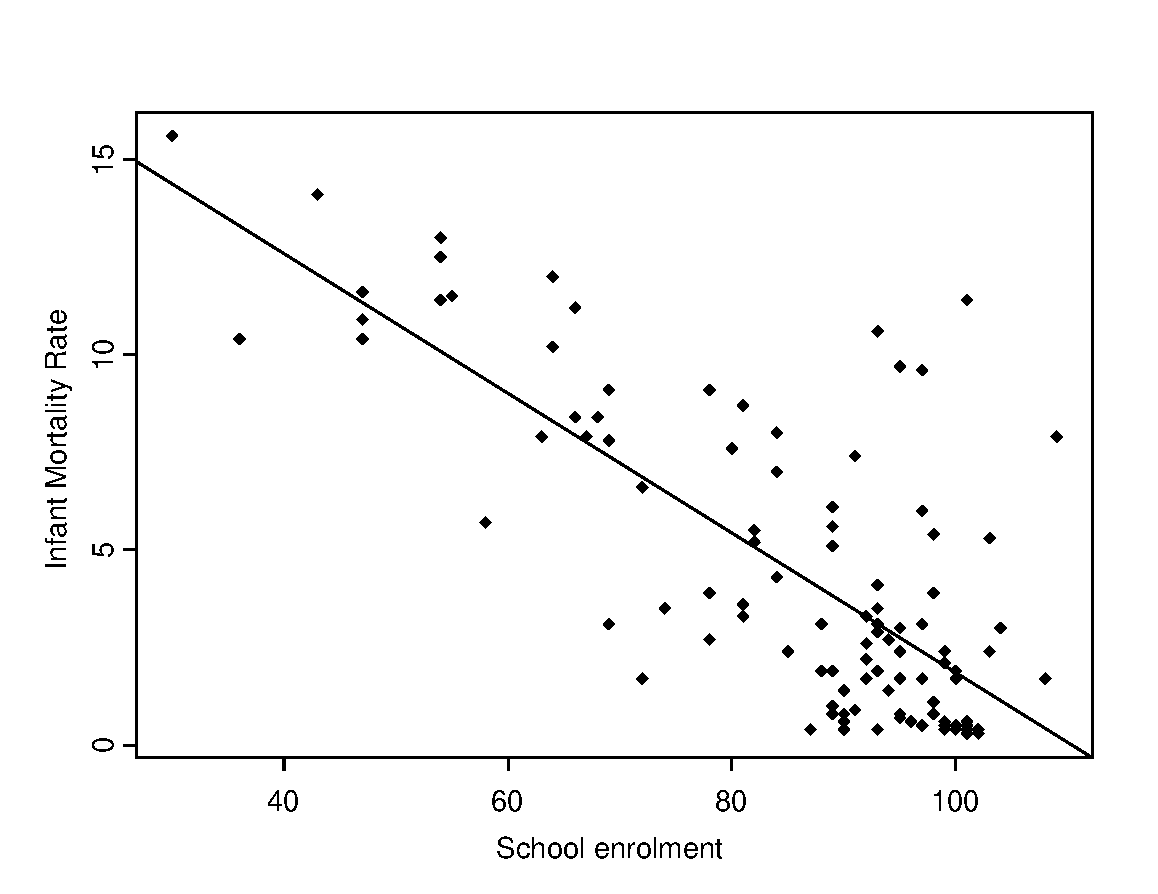
\includegraphics[width=13.50000cm]{imr1.pdf}
\caption{\label{fig:f-imr1} A scatterplot of net primary school enrolment
ratio vs.~Infant mortality rate for countries in the Global Civil
Society data set (\(n=111\)). The solid line is the best-fitting (least
squares) straight line for the points.}
\end{figure}

\begin{longtable}[]{@{}lrrrr@{}}
\caption{\label{tab:t-imrvars} Summary statistics for Infant Mortality Rate
(IMR) and explanatory variables for it considered in the examples of
Sections \ref{s-regression-simple} and \ref{s-regression-multiple}
(\(n=111\)). See Example 8.1 for further information on the
variables.}\tabularnewline
\toprule
\begin{minipage}[t]{0.41\columnwidth}\raggedright\strut
\strut
\end{minipage} & \begin{minipage}[t]{0.20\columnwidth}\raggedleft\strut
IMR\strut
\end{minipage} & \begin{minipage}[t]{0.07\columnwidth}\raggedleft\strut
School enrolment\strut
\end{minipage} & \begin{minipage}[t]{0.08\columnwidth}\raggedleft\strut
Control of corruption\strut
\end{minipage} & \begin{minipage}[t]{0.08\columnwidth}\raggedleft\strut
Income inequality\strut
\end{minipage}\tabularnewline
\begin{minipage}[t]{0.41\columnwidth}\raggedright\strut
\emph{Summary statistics}\strut
\end{minipage} & \begin{minipage}[t]{0.20\columnwidth}\raggedleft\strut
\strut
\end{minipage} & \begin{minipage}[t]{0.07\columnwidth}\raggedleft\strut
\strut
\end{minipage} & \begin{minipage}[t]{0.08\columnwidth}\raggedleft\strut
\strut
\end{minipage} & \begin{minipage}[t]{0.08\columnwidth}\raggedleft\strut
\strut
\end{minipage}\tabularnewline
\begin{minipage}[t]{0.41\columnwidth}\raggedright\strut
Mean\strut
\end{minipage} & \begin{minipage}[t]{0.20\columnwidth}\raggedleft\strut
4.3\strut
\end{minipage} & \begin{minipage}[t]{0.07\columnwidth}\raggedleft\strut
86.1\strut
\end{minipage} & \begin{minipage}[t]{0.08\columnwidth}\raggedleft\strut
50.1\strut
\end{minipage} & \begin{minipage}[t]{0.08\columnwidth}\raggedleft\strut
40.5\strut
\end{minipage}\tabularnewline
\begin{minipage}[t]{0.41\columnwidth}\raggedright\strut
std.~deviation\strut
\end{minipage} & \begin{minipage}[t]{0.20\columnwidth}\raggedleft\strut
4.0\strut
\end{minipage} & \begin{minipage}[t]{0.07\columnwidth}\raggedleft\strut
16.7\strut
\end{minipage} & \begin{minipage}[t]{0.08\columnwidth}\raggedleft\strut
28.4\strut
\end{minipage} & \begin{minipage}[t]{0.08\columnwidth}\raggedleft\strut
10.2\strut
\end{minipage}\tabularnewline
\begin{minipage}[t]{0.41\columnwidth}\raggedright\strut
Minimum\strut
\end{minipage} & \begin{minipage}[t]{0.20\columnwidth}\raggedleft\strut
0.3\strut
\end{minipage} & \begin{minipage}[t]{0.07\columnwidth}\raggedleft\strut
30.0\strut
\end{minipage} & \begin{minipage}[t]{0.08\columnwidth}\raggedleft\strut
3.6\strut
\end{minipage} & \begin{minipage}[t]{0.08\columnwidth}\raggedleft\strut
24.4\strut
\end{minipage}\tabularnewline
\begin{minipage}[t]{0.41\columnwidth}\raggedright\strut
Maximum\strut
\end{minipage} & \begin{minipage}[t]{0.20\columnwidth}\raggedleft\strut
15.6\strut
\end{minipage} & \begin{minipage}[t]{0.07\columnwidth}\raggedleft\strut
109.0\strut
\end{minipage} & \begin{minipage}[t]{0.08\columnwidth}\raggedleft\strut
100.0\strut
\end{minipage} & \begin{minipage}[t]{0.08\columnwidth}\raggedleft\strut
70.7\strut
\end{minipage}\tabularnewline
\begin{minipage}[t]{0.41\columnwidth}\raggedright\strut
\emph{Correlation matrix}\strut
\end{minipage} & \begin{minipage}[t]{0.20\columnwidth}\raggedleft\strut
\strut
\end{minipage} & \begin{minipage}[t]{0.07\columnwidth}\raggedleft\strut
\strut
\end{minipage} & \begin{minipage}[t]{0.08\columnwidth}\raggedleft\strut
\strut
\end{minipage} & \begin{minipage}[t]{0.08\columnwidth}\raggedleft\strut
\strut
\end{minipage}\tabularnewline
\begin{minipage}[t]{0.41\columnwidth}\raggedright\strut
IMR\strut
\end{minipage} & \begin{minipage}[t]{0.20\columnwidth}\raggedleft\strut
1\strut
\end{minipage} & \begin{minipage}[t]{0.07\columnwidth}\raggedleft\strut
-0.75\strut
\end{minipage} & \begin{minipage}[t]{0.08\columnwidth}\raggedleft\strut
-0.60\strut
\end{minipage} & \begin{minipage}[t]{0.08\columnwidth}\raggedleft\strut
0.39\strut
\end{minipage}\tabularnewline
\begin{minipage}[t]{0.41\columnwidth}\raggedright\strut
School enrolment\strut
\end{minipage} & \begin{minipage}[t]{0.20\columnwidth}\raggedleft\strut
-0.75\strut
\end{minipage} & \begin{minipage}[t]{0.07\columnwidth}\raggedleft\strut
1\strut
\end{minipage} & \begin{minipage}[t]{0.08\columnwidth}\raggedleft\strut
0.39\strut
\end{minipage} & \begin{minipage}[t]{0.08\columnwidth}\raggedleft\strut
-0.27\strut
\end{minipage}\tabularnewline
\begin{minipage}[t]{0.41\columnwidth}\raggedright\strut
Control of corruption\strut
\end{minipage} & \begin{minipage}[t]{0.20\columnwidth}\raggedleft\strut
-0.60\strut
\end{minipage} & \begin{minipage}[t]{0.07\columnwidth}\raggedleft\strut
0.39\strut
\end{minipage} & \begin{minipage}[t]{0.08\columnwidth}\raggedleft\strut
1\strut
\end{minipage} & \begin{minipage}[t]{0.08\columnwidth}\raggedleft\strut
-0.27\strut
\end{minipage}\tabularnewline
\begin{minipage}[t]{0.41\columnwidth}\raggedright\strut
Income inequality\strut
\end{minipage} & \begin{minipage}[t]{0.20\columnwidth}\raggedleft\strut
0.39\strut
\end{minipage} & \begin{minipage}[t]{0.07\columnwidth}\raggedleft\strut
-0.27\strut
\end{minipage} & \begin{minipage}[t]{0.08\columnwidth}\raggedleft\strut
-0.27\strut
\end{minipage} & \begin{minipage}[t]{0.08\columnwidth}\raggedleft\strut
1\strut
\end{minipage}\tabularnewline
\begin{minipage}[t]{0.41\columnwidth}\raggedright\strut
\emph{Means for countries in different income categories}\strut
\end{minipage} & \begin{minipage}[t]{0.20\columnwidth}\raggedleft\strut
\strut
\end{minipage} & \begin{minipage}[t]{0.07\columnwidth}\raggedleft\strut
\strut
\end{minipage} & \begin{minipage}[t]{0.08\columnwidth}\raggedleft\strut
\strut
\end{minipage} & \begin{minipage}[t]{0.08\columnwidth}\raggedleft\strut
\strut
\end{minipage}\tabularnewline
\begin{minipage}[t]{0.41\columnwidth}\raggedright\strut
Low income (\(n=41\))\strut
\end{minipage} & \begin{minipage}[t]{0.20\columnwidth}\raggedleft\strut
8.2\strut
\end{minipage} & \begin{minipage}[t]{0.07\columnwidth}\raggedleft\strut
72.1\strut
\end{minipage} & \begin{minipage}[t]{0.08\columnwidth}\raggedleft\strut
27.5\strut
\end{minipage} & \begin{minipage}[t]{0.08\columnwidth}\raggedleft\strut
41.7\strut
\end{minipage}\tabularnewline
\begin{minipage}[t]{0.41\columnwidth}\raggedright\strut
Middle income (\(n=48\))\strut
\end{minipage} & \begin{minipage}[t]{0.20\columnwidth}\raggedleft\strut
2.8\strut
\end{minipage} & \begin{minipage}[t]{0.07\columnwidth}\raggedleft\strut
92.5\strut
\end{minipage} & \begin{minipage}[t]{0.08\columnwidth}\raggedleft\strut
50.8\strut
\end{minipage} & \begin{minipage}[t]{0.08\columnwidth}\raggedleft\strut
43.3\strut
\end{minipage}\tabularnewline
\begin{minipage}[t]{0.41\columnwidth}\raggedright\strut
High income (\(n=22\))\strut
\end{minipage} & \begin{minipage}[t]{0.20\columnwidth}\raggedleft\strut
0.5\strut
\end{minipage} & \begin{minipage}[t]{0.07\columnwidth}\raggedleft\strut
98.4\strut
\end{minipage} & \begin{minipage}[t]{0.08\columnwidth}\raggedleft\strut
90.7\strut
\end{minipage} & \begin{minipage}[t]{0.08\columnwidth}\raggedleft\strut
32.0\strut
\end{minipage}\tabularnewline
\bottomrule
\end{longtable}

\subsection{Definition of the model}\label{ss-regression-simple-def}

The simple linear regression model defined in this section is a
statistical model for a continuous, interval level response variable
\(Y\) given a single explanatory variable \(X\), such as IMR given
School enrolment. The model will be used to carry out statistical
inference on the association between the variables in a population
(which in the IMR example is clearly again of the conceptual variety).

For motivation, recall first the situation considered in Section
\ref{s-means-inference}. There the data consisted of observations
\((Y_{i}, X_{i})\) for \(i=1,2,\dots,n\), which were assumed to be
statistically independent. The response variable \(Y\) was continuous
but \(X\) had only two possible values, coded 1 and 2. A model was then
set up where the population distribution of \(Y\) had mean \(\mu_{1}\)
and variance \(\sigma^{2}_{1}\) for units with \(X=1\), and mean
\(\mu_{2}\) and variance \(\sigma^{2}_{2}\) when \(X=2\). In some cases
it was further assumed that the population distributions were both
normal, and that the population variances were equal, i.e.~that
\(\sigma^{2}_{1}=\sigma^{2}_{2}\), with their common value denoted
\(\sigma^{2}\). With these further assumptions, which will also be used
here, the model for \(Y\) given a dichotomous \(X\) stated that (1)
observations for different units \(i\) were statistically independent;
(2) each \(Y_{i}\) was sampled at random from a population distribution
which was normal with mean \(\mu_{i}\) and variance \(\sigma^{2}\); and
(3) \(\mu_{i}\) depended on \(X_{i}\) so that it was equal to
\(\mu_{1}\) if \(X_{i}\) was 1 and \(\mu_{2}\) if \(X_{i}\) was 2.

The situation in this section is exactly the same, except that \(X\) is
now continuous instead of dichotomous. We will use the same basic model,
but will change the specification of the conditional mean \(\mu_{i}\)
appropriately. In the light of the discussion in previous sections of
this chapter, it is no surprise that this will be defined in such a way
that it describes a linear association between \(X\) and \(Y\). This is
done by setting \(\mu_{i}=\alpha+\beta X_{i}\), where \(\alpha\) and
\(\beta\) are unknown population parameters. This is the equation of
straight line (we will return to it in the next section). With this
specification, the model for observations
\((Y_{1},X_{1}), (Y_{2}, X_{2}), \dots, (Y_{n}, X_{n})\) becomes

\begin{enumerate}
\def\labelenumi{\arabic{enumi}.}
\item
  Observations for different units \(i\) (\(=1,2,\dots,n\)) are
  statistically independent.
\item
  Each \(Y_{i}\) is normally distributed with mean \(\mu_{i}\) and
  variance \(\sigma^{2}\).
\item
  The means \(\mu_{i}\) depend on \(X_{i}\) through
  \(\mu_{i}=\alpha+\beta X_{i}\).
\end{enumerate}

Often the model is expressed in an equivalent form where 2.~and 3.~are
combined as

\begin{equation}Y_{i}=\alpha+\beta X_{i} +\epsilon_{i}
\label{eq:slinmodel}\end{equation}

where each \(\epsilon_{i}\) is normally distributed with mean 0 and
variance \(\sigma^{2}\). The \(\epsilon_{i}\) are known as \textbf{error
terms} or \textbf{population residuals} (and the letter \(\epsilon\) is
the lower-case Greek ``epsilon''). This formulation of the model clearly
separates the mean of \(Y_{i}\), which traces the straight line
\(\alpha+\beta X_{i}\) as \(X_{i}\) changes, from the variation around
that line, which is described by the variability of \(\epsilon_{i}\).

The model defined above is known as the \textbf{simple linear regression
model}:

\begin{itemize}
\item
  \textbf{Simple} because it has only one explanatory variable, as
  opposed to \emph{multiple} linear regression models which will have
  more than one.
\item
  \textbf{Linear} because it specifies a linear association between
  \(X\) and \(Y\).\footnote{The data can be obtained from
    \texttt{www3.norc.org/GSS+Website/}, which gives further information
    on the survey, including the full text of the questionnaires.}
\item
  \textbf{Regression}: This is now an established part of the name of
  the model, although the origins of the word are not central to the use
  of the model\footnote{United Nations Development Programme
    \emph{International Human Development Indicators},
    \texttt{http://hdr.undp.org/en/data/}; World Bank \emph{Worldwide
    Governance Indicators},
    \texttt{http://info.worldbank.org/governance/wgi/pdf/wgidataset.xlsx};
    World Bank \emph{World Development Indicators},
    \texttt{http://data.worldbank.org/indicator/SP.DYN.IMRT.IN}.}.
\item
  \textbf{Model}, because this is a statistical model in the sense
  discussed in the middle of Section \ref{ss-contd-probdistrs-general}.
  In other words, the model is always only a simplified abstraction of
  the true, immeasurably complex processes which determine the values of
  \(Y\). Nevertheless, it is believed that a well-chosen model can be
  useful for explaining and predicting observed values of \(Y\). This
  spirit is captured by the well-known statement by the statistician
  George Box\footnote{ESS Round 5: European Social Survey Round 5 Data
    (2010). Data file edition 2.0. Norwegian Social Science Data
    Services, Norway � Data Archive and distributor of ESS data. The
    full data can be obtained from
    \texttt{http://ess.nsd.uib.no/ess/round5/}.}:

  \begin{quote}
  \emph{All models are wrong, but some are useful.}
  \end{quote}

  A model like this has the advantage that it reduces the examination of
  associations in the population to estimation and inference on a small
  number of model parameters, in the case of the simple linear
  regression model just \(\alpha\), \(\beta\) and \(\sigma^{2}\).
\end{itemize}

Of course, not all models are equally appropriate for given data, and
some will be both wrong and useless. The results from a model should
thus be seriously presented and interpreted only if the model is deemed
to be reasonably adequate. For the simple linear regression model, this
can be partly done by examining whether the scatterplot between \(X\)
and \(Y\) appears to be reasonably consistent with a linear
relationship. Some further comments on the assessment of model adequacy
will be given in Section \ref{s-regression-rest}.

\subsection{Interpretation of the model
parameters}\label{ss-regression-simple-int}

The simple linear regression model (\ref{eq:slinmodel}) has three
parameters, \(\alpha\), \(\beta\) and \(\sigma^{2}\). Each of these has
its own interpretation, which are explained in this section. Sometimes
it will be useful to illustrate the definition with specific numerical
values, for which we will use ones for the model for IMR given School
enrolment in our example. SPSS output for this model is shown in Figure
\ref{fig:f-spss-linreg}. Note that although these values are first used
here to illustrate the interpretation of the \emph{population}
parameters in the model, they are of course only estimates (of a kind
explained in the next section) of those parameters. Other parts of the
SPSS output will be explained later in this chapter.

\begin{figure}[htbp]
\centering
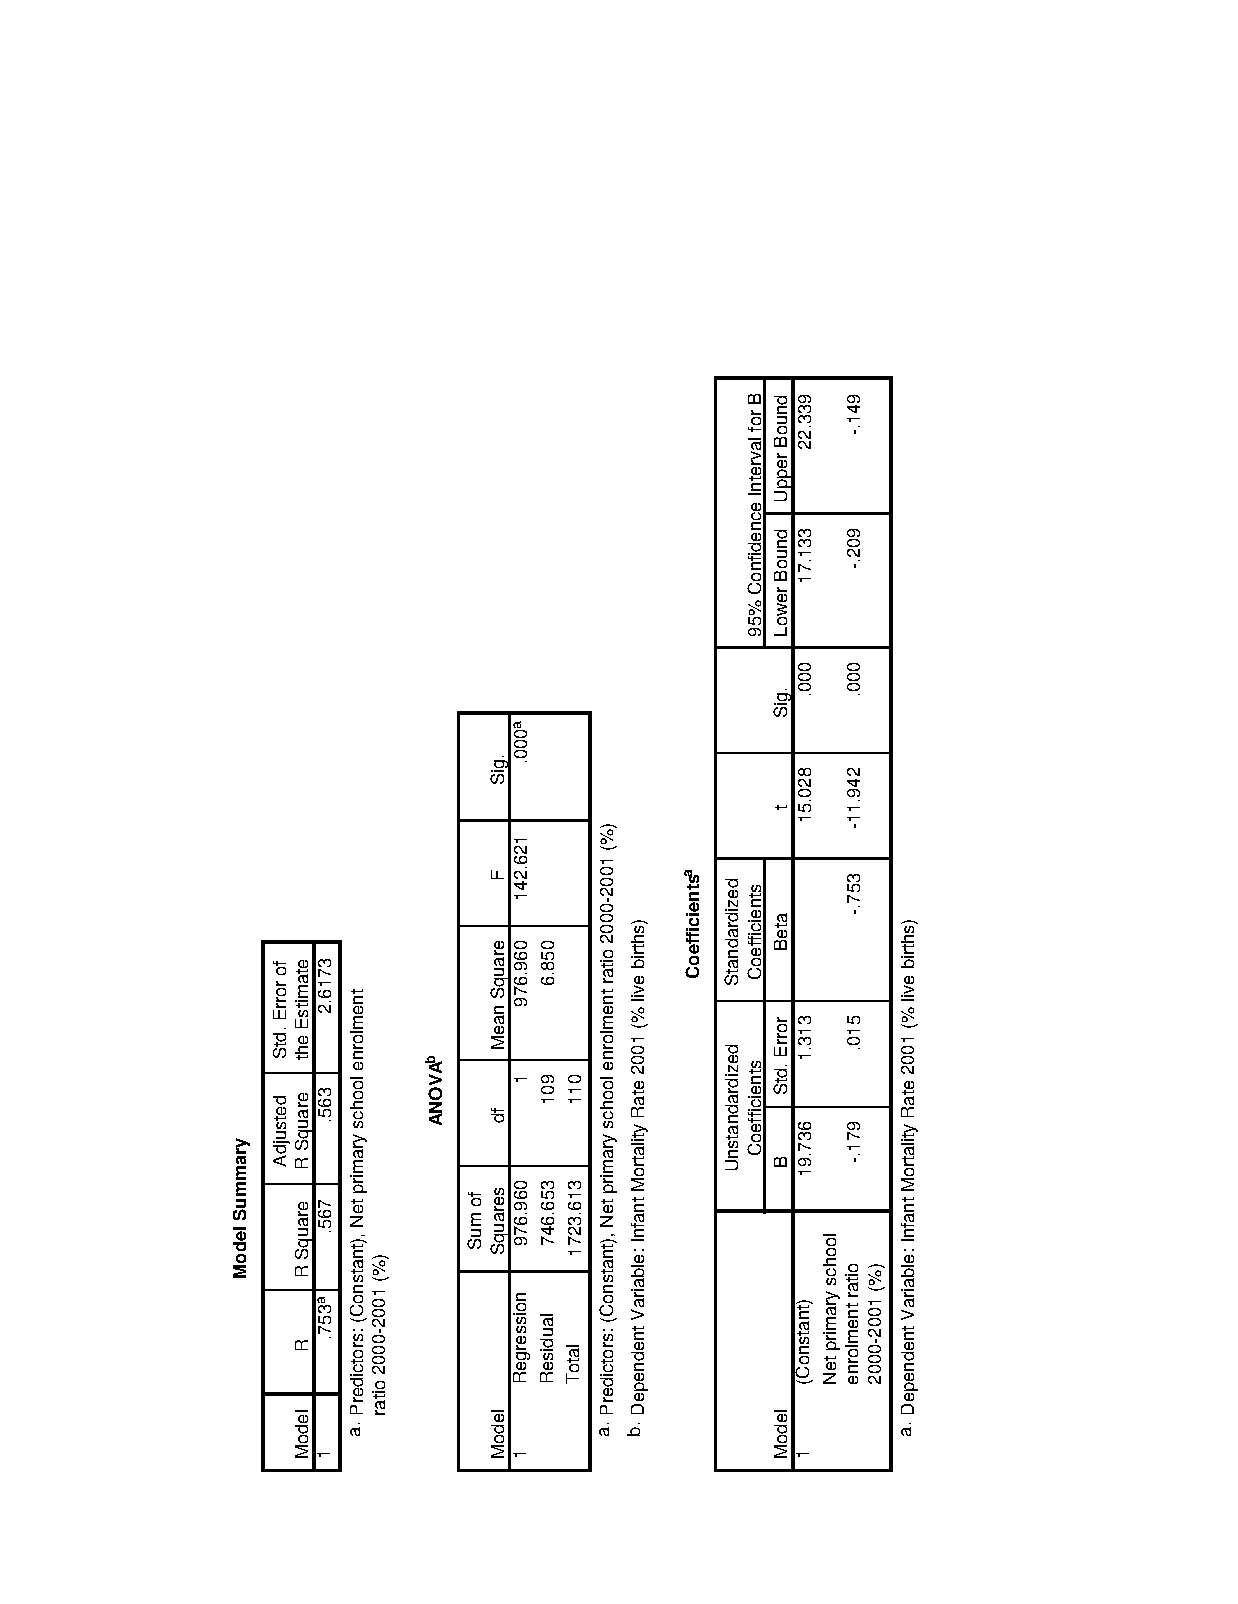
\includegraphics[width=15.50000cm]{spsslinreg.pdf}
\caption{\label{fig:f-spss-linreg} SPSS output for a simple linear
regression model for Infant mortality rate given School enrolment in the
Global Civil Society data.}
\end{figure}

According to the model, the conditional mean (also often known as the
conditional \textbf{expected value}) of \(Y\) given \(X\) in the
population is (dropping the subscript \(i\) for now for notational
simplicity) \(\mu=\alpha+\beta X\). The two parameters \(\alpha\) and
\(\beta\) in this formula are known as \textbf{regression coefficients}.
They are interpreted as follows:

\begin{itemize}
\item
  \(\alpha\) is the expected value of \(Y\) when \(X\) is equal to 0. It
  is known as the \textbf{intercept} or \textbf{constant} term of the
  model.
\item
  \(\beta\) is the change in the expected value of \(Y\) when \(X\)
  increases by 1 unit. It is known as the \textbf{slope} term or the
  \textbf{coefficient of} \(X\).
\end{itemize}

Just to include one mathematical proof in this coursepack, these results
can be derived as follows:

\begin{itemize}
\item
  When \(X=0\), the mean of \(Y\) is
  \(\mu=\alpha+\beta X=\alpha+\beta\times 0 =\alpha+0=\alpha\).
\item
  Compare two observations, one with value \(X\) of the explanatory
  variable, and the other with one unit more, i.e.~\(X+1\). The
  corresponding means of \(Y\) are

  \begin{longtable}[]{@{}rlll@{}}
  \toprule
  with \(X+1\): & \(\mu\) & \(=\alpha+\beta\times (X+1)\) &
  \(=\alpha+\beta X +\beta\)\tabularnewline
  with \(X\): & \(\mu\) & & \(=\alpha+\beta X\)\tabularnewline
  Difference: & & & \(\beta\)\tabularnewline
  \bottomrule
  \end{longtable}
\end{itemize}

which completes the proof of the claims above --- Q.E.D. In case you
prefer a graphical summary, this is given in Figure
\ref{fig:f-linmod-params}.

\begin{figure}[htbp]
\centering
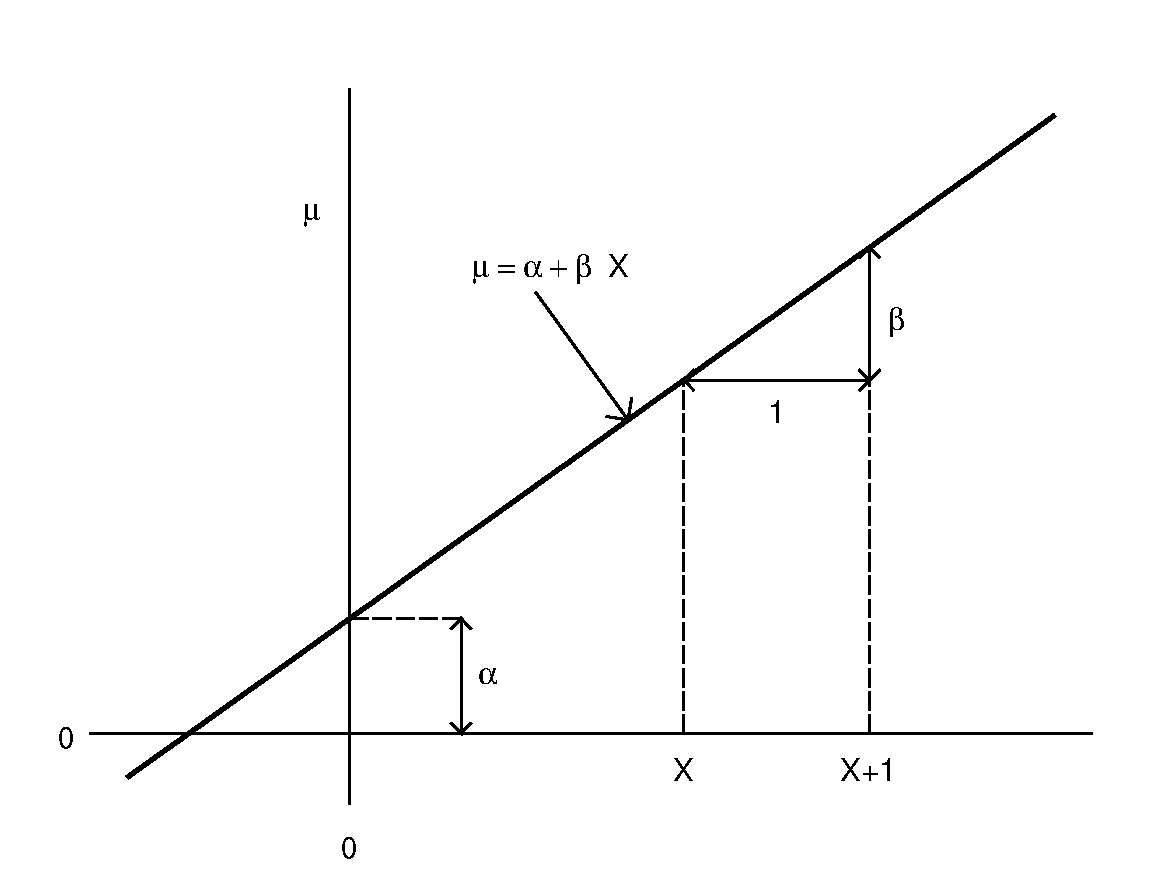
\includegraphics[width=12.50000cm]{lmparams.pdf}
\caption{\label{fig:f-linmod-params} Illustration of the interpretation of
the regression coefficients of a simple linear regression model.}
\end{figure}

The most important parameter of the model, and usually the only one
really discussed in interpreting the results, is \(\beta\), the
regression coefficient of \(X\). It is also called the slope because it
is literally the slope of the regression line, as shown in Figure
\ref{fig:f-linmod-params}. It is the only parameter in the model which
describes the association between \(X\) and \(Y\), and it does so in the
above terms of expected changes in \(Y\) corresponding to changes in X
(\(\beta\) is also related to the correlation between \(X\) and \(Y\),
in a way explained in the next section). The sign of \(\beta\) indicates
the direction of the association. When \(\beta\) is positive (greater
than 0), the regression line slopes upwards and increasing \(X\) thus
also increases the expected value of \(Y\) --- in other words, the
association between \(X\) and \(Y\) is positive. This is the case
illustrated in Figure \ref{fig:f-linmod-params}. If \(\beta\) is
negative, the regression line slopes downwards and the association is
also negative. Finally, if \(\beta\) is zero, the line is parallel with
the \(X\)-axis, so that changing \(X\) does not change the expected
value of \(Y\). Thus \(\beta=0\) corresponds to no (linear) association
between \(X\) and \(Y\).

In the real example shown in Figure \ref{fig:f-spss-linreg}, \(X\) is
School enrolment and \(Y\) is IMR. In SPSS output, the estimated
regression coefficients are given in the ``\textbf{Coefficients}'' table
in the column labelled ``B'' under ``Unstandardized coefficients''. The
estimated constant term \(\alpha\) is given in the row labelled
``(Constant)'', and the slope term on the next row, labelled with the
name or label of the explanatory variable as specified in the SPSS data
file --- here ``Net primary school enrolment ratio 2000-2001 (\%)''. The
value of the intercept is here 19.736 and the slope coefficient is
\(-0.179\). The estimated regression line for expected IMR is thus
\(19.736-0.179 X\), where \(X\) denotes School enrolment. This is the
line shown in Figure \ref{fig:f-imr1}.

Because the slope coefficient in the example is negative, the
association between the variables is also negative, i.e.~higher levels
of school enrolment are associated with lower levels of infant
mortality. More specifically, every increase of one unit (here one
percentage point) in School enrolment is associated with a decrease of
0.179 units (here percentage points) in expected IMR.

Since the meaning of \(\beta\) is related to a unit increase of the
explanatory variable, the interpretation of its magnitude depends on
what those units are. In many cases one unit of \(X\) is too small or
too large for convenient interpretation. For example, a change of one
percentage point in School enrolment is rather small, given that the
range of this variable in our data is 79 percentage points (c.f.~Table
\ref{tab:t-imrvars}). In such cases the results can easily be
reexpressed by using multiples of \(\beta\): specifically, the effect on
expected value of \(Y\) of changing \(X\) by \(A\) units is obtained by
multiplying \(\beta\) by \(A\). For instance, in our example the
estimated effect of increasing School enrolment by 10 percentage points
is to decrease expected IMR by \(10\times 0.179=1.79\) percentage
points.

The constant term \(\alpha\) is a necessary part of the model, but it is
almost never of interest in itself. This is because the expected value
of \(Y\) at \(X=0\) is rarely specifically interesting. Very often
\(X=0\) is also unrealistic, as in our example where it corresponds to a
country with zero primary school enrolment. There are fortunately no
such countries in the data, where the lowest School enrolment is 30\%.
It is then of no interest to discuss expected IMR for a hypothetical
country where no children went to school. Doing so would also represent
unwarranted \emph{extrapolation} of the model beyond the range of the
observed data. Even though the estimated linear model seems to fit
reasonably well for these data, this is no guarantee that it would do so
also for countries with much lower school enrolment, even if they
existed.

The third parameter of the simple regression model is \(\sigma^{2}\).
This is the variance of the conditional distribution of \(Y\) given
\(X\). It is also known as the \textbf{conditional variance} of \(Y\),
the \textbf{error variance} or the \textbf{residual variance}.
Similarly, its square root \(\sigma\) is known as the conditional, error
or \textbf{residual standard deviation}. To understand \(\sigma\), let
us consider a single value of \(X\), such as one corresponding to one of
the vertical dashed lines in Figure \ref{fig:f-linmod-params} or, say,
school enrolment of 85 in Figure \ref{fig:f-imr1}. The model specifies a
distribution for \(Y\) given any such value of \(X\). If we were to
(hypothetically) collect a large number of observations, all with this
same value of \(X\), the distribution of \(Y\) for them would describe
the conditional distribution of \(Y\) given that value of \(X\). The
model states that the average of these values, i.e.~the conditional mean
of \(Y\), is \(\alpha+\beta X\), which is the point on the regression
line corresponding to \(X\). The individual values of \(Y\), however,
would of course not all be on the line but somewhere around it, some
above and some below.

The linear regression model further specifies that the form of the
conditional distribution of \(Y\) is approximately normal. You can try
to visualise this by imagining a normal probability curve (c.f.~Figure
\ref{fig:f-norm1}) on the vertical line from \(X\), centered on the
regression line and sticking up from the page. The bell shape of the
curve indicates that most of the values of \(Y\) for a given \(X\) will
be close to the regression line, and only small proportions of them far
from it. The residual standard deviation \(\sigma\) is the standard
deviation of this conditional normal distribution, in essence describing
how tightly concentrated values of \(Y\) tend to be around the
regression line. The model assumes, mainly for simplicity, that the same
value of \(\sigma\) applies to the conditional distributions at all
values of \(X\); this is known as the assumption of
\emph{homoscedasticity}.

In SPSS output, an estimate of \(\sigma\) is given in the
``\textbf{Model Summary}'' table under the misleading label ``Std.~Error
of the Estimate''. An estimate of the residual variance \(\sigma^{2}\)
is found also in the ``\textbf{ANOVA}'' table under ``Mean Square'' for
``Residual''. In our example the estimate of \(\sigma\) is 2.6173 (and
that of \(\sigma^{2}\) is 6.85). This is usually not of direct interest
for interpretation, but it will be a necessary component of some parts
of the analysis discussed below.

\subsection{Estimation of the
parameters}\label{ss-regression-simple-est}

Since the regression coefficients \(\alpha\) and \(\beta\) and the
residual standard deviation \(\sigma\) are unknown population
parameters, we will need to use the observed data to obtain sensible
estimates for them. How to do so is now less obvious than in the cases
of simple means and proportions considered before. This section explains
the standard method of estimation for the parameters of linear
regression models.

We will denote estimates of \(\alpha\) and \(\beta\) by \(\hat{\alpha}\)
and \(\hat{\beta}\) (``alpha-hat'' and ``beta-hat'') respectively (other
notations are also often used, e.g.~\(a\) and \(b\)). Similarly, we can
define \[\hat{Y}=\hat{\alpha}+\hat{\beta} X\] for \(Y\) given any value
of \(X\). These are the values on the estimated regression line. They
are known as \textbf{fitted values} for \(Y\), and estimating the
parameters of the regression model is often referred to as ``fitting the
model'' to the observed data. The fitted values represent our
predictions of expected values of \(Y\) given \(X\), so they are also
known as \textbf{predicted values} of \(Y\).

In particular, fitted values
\(\hat{Y}_{i}=\hat{\alpha}+\hat{\beta}X_{i}\) can be calculated at the
values \(X_{i}\) of the explanatory variable \(X\) for each unit \(i\)
in the observed sample. These can then be compared to the correponding
values \(Y_{i}\) of the response variable. Their differences
\(Y_{i}-\hat{Y}_{i}\) are known as the (sample) \textbf{residuals}.
These quantities are illustrated in Figure \ref{fig:f-residuals}. This
shows a fitted regression line, which is in fact the one for IMR given
School enrolment also shown in Figure \ref{fig:f-imr1}. Also shown are
two points \((X_{i}, Y_{i})\). These are also from Figure
\ref{fig:f-imr1}; the rest have been omitted to simplify the plot. The
point further to the left is the one for Mali, which has School
enrolment \(X_{i}=43.0\) and IMR \(Y_{i}=14.1\). Using the estimated
coefficients \(\hat{\alpha}=19.736\) and \(\hat{\beta}=-0.179\) in
Figure \ref{fig:f-spss-linreg}, the fitted value for Mali is
\(\hat{Y}_{i}=19.736-0.179\times 43.0=12.0\). Their difference is the
residual \(Y_{i}-\hat{Y}_{i}=14.1-12.0=2.1\). Because the observed value
is here larger than the fitted value, the residual is positive and the
observed value is above the fitted line, as shown in Figure
\ref{fig:f-residuals}.

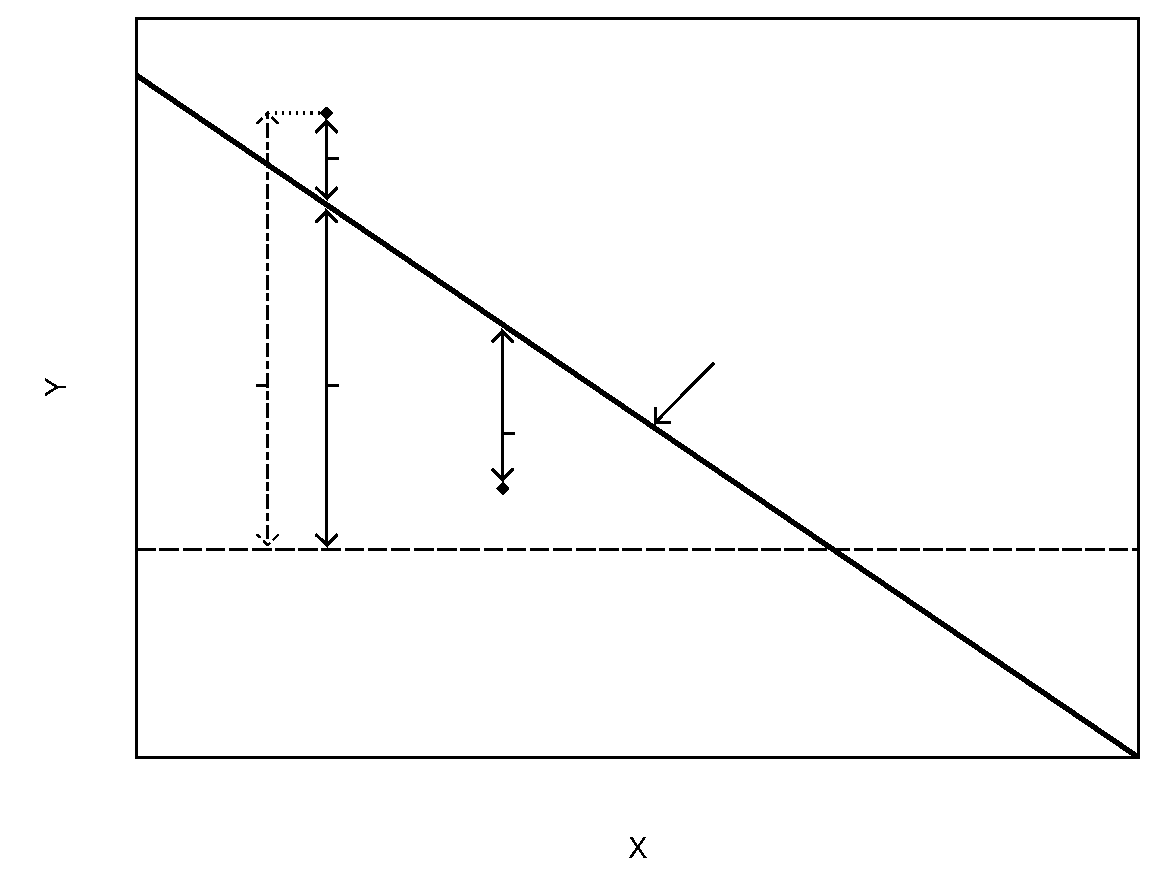
\includegraphics[width=13.50000cm]{lmresids.pdf} The second point shown
in Figure \ref{fig:f-residuals} corresponds to the observation for
Ghana, for which \(X_{i}=58.0\) and \(Y_{i}=5.7\). The fitted value is
then \(\hat{Y}_{i}=19.736-0.179\times 58.0=9.4\) and the residual
\(Y_{i}-\hat{Y}_{i}=5.7-9.4=-3.7\). Because the observed value is now
smaller than the fitted value, the residual is negative and the observed
\(Y_{i}\) is below the fitted regression line.

So far we have still not explained how the specific values of the
parameter estimates in Figure \ref{fig:f-spss-linreg} were obtained. In
doing so, we are faced with the task of identifying a regression line
which provides the best fit to the observed points in a scatterplot like
Figure \ref{fig:f-imr1}. Each possible choice of \(\hat{\alpha}\) and
\(\hat{\beta}\) corresponds to a different regression line, and some
choices are clearly better than others. For example, it seems
intuitively obvious that it would be better for the line to go through
the cloud of points rather than stay completely outside it. To make such
considerations explicit, the residuals can be used as a criterion of
model fit. The aim will then be to make the total magnitude of the
residuals as small as possible, so that the fitted line is as close as
possible to the observed points \(Y_{i}\) in some overall sense. This
cannot be done simply by adding up the residuals, because they can have
different signs, and positive and negative residuals could thus cancel
out each other in the addition. As often before, the way around this is
to remove the signs by considering the squares of the residuals. Summing
these over all units \(i\) in the sample leads to the sum of squared
residuals \[SSE = \sum (Y_{i}-\hat{Y}_{i})^{2}.\] Here \(SSE\) is short
for Sum of Squares of Errors (it is also often called the Residual Sum
of Squares or \(RSS\)). This is the quantity used as the criterion in
estimating regression coefficients for a linear model. Different
candidate values for \(\hat{\alpha}\) and \(\hat{\beta}\) lead to
different values of \(\hat{Y}_{i}\) and thus of \(SSE\). The final
estimates are the ones which give the smallest value of \(SSE\). Their
formulas are

\begin{equation}\hat{\beta}=
\frac{
\sum (X_{i}-\bar{X})(Y_{i}-\bar{Y})}
{\sum (X_{i}-\bar{X})^{2}}
=\frac{s_{xy}}{s_{x}^{2}}
\label{eq:ols-b}\end{equation}

and

\begin{equation}\hat{\alpha}=\bar{Y}-\hat{\beta}\bar{X}
\label{eq:ols-a}\end{equation}

where \(\bar{Y}\), \(\bar{X}\), \(s_{x}\) and \(s_{xy}\) are the usual
sample means, standard deviations and covariances for \(Y\) and \(X\).
These are known as the \textbf{least squares estimates} of the
regression coefficients (or as Ordinary Least Squares or OLS estimates),
and the reasoning used to obtain them is the \textbf{method of least
squares}\footnote{This is another old idea. Different approaches to the
  problem of fitting curves to observations were gradually developed by
  Tobias Mayer, Rudjer Bošković and Pierre Simon Laplace from the 1750s
  onwards, and the method of least squares itself was presented by
  Adrien Marie Legendre in 1805.}. Least squares estimates are almost
always used for linear regression models, and they are the ones
displayed by SPSS and other software. For our model for IMR given School
enrolment, the estimates are the \(\hat{\alpha}=19.736\) and
\(\hat{\beta}=-0.179\) shown in Figure \ref{fig:f-spss-linreg}.

The estimated coefficients can be used to calculate predicted values for
\(Y\) at any values of \(X\), not just those included in the observed
sample. For instance, in the infant mortality example the predicted IMR
for a country with School enrolment of 80\% would be
\(\hat{Y}=19.736-0.179\times 80=5.4\). Such predictions should usually
be limited to the range of values of \(X\) actually observed in the
data, and extrapolation beyond these values should be avoided.

The most common estimate of the remaining parameter of the model, the
residual standard deviation \(\sigma\), is

\begin{equation}\hat{\sigma}=
\sqrt{
\frac{\sum (Y_{i}-\hat{Y}_{i})^{2}}{n-(k+1)}
}
=\sqrt{
\frac{SSE}{n-(k+1)}
}
\label{eq:sigma-linreg}\end{equation}

where \(k\) is here set equal to 1. This bears an obvious resemblance to
the formula for the basic sample standard deviation, shown for \(Y_{i}\)
in (\ref{eq:sdyx}). One difference to that formula is that the
denominator of (\ref{eq:sigma-linreg}) is shown as \(n-(k+1)\) rather
than \(n-1\). Here \(k=1\) is the number of explanatory variables in the
model, and \(k+1=2\) is the number of regression coefficients
(\(\alpha\) and \(\beta\)) including the constant term \(\alpha\). The
quantity \(n-(k+1)\), i.e.~here \(n-2\), is the \textbf{degrees of
freedom} (\(df\)) of the parameter estimates. We will need it again in
the next section. It is here given in the general form involving the
symbol \(k\), so that we can later refer to the same formula for models
with more explanatory variables and thus \(k\) greater than 1. In SPSS
output, the degrees of freedom are shown in the ``\textbf{ANOVA}'' table
under ``df'' for ``Residual''. In the infant mortality example
\(n=111\), \(k=1\) and \(df=111-2=109\), as shown in Figure
\ref{fig:f-spss-linreg}.

Finally, two connections between previous topics and the parameters
\(\hat{\alpha}\), \(\hat{\beta}\) and \(\hat{\sigma}\) are worth
highlighting:

\begin{itemize}
\item
  The estimated slope \(\hat{\beta}\) from (\ref{eq:ols-b}) is related
  to the sample correlation \(r\) from (\ref{eq:corr}) by
  \(r=(s_{x}/s_{y})\,\hat{\beta}\). In both of these it is
  \(\hat{\beta}\) which carries information about the association
  between \(X\) and \(Y\). The ratio \(s_{x}/s_{y}\) serves only to
  standardise the correlation coefficient so that it is always between
  \(-1\) and \(+1\). The slope coefficient \(\hat{\beta}\) is not
  standardised, and the interpretation of its magnitude depends on the
  units of measurement of \(X\) and \(Y\) in the way defined in Section
  \ref{ss-regression-simple-int}.
\item
  Suppose we simplify the simple linear regression model
  (\ref{eq:slinmodel}) further by setting \(\beta=0\), thus removing
  \(\beta X\) from the model. The new model states that all \(Y_{i}\)
  are normally distributed with the same mean \(\alpha\) and standard
  deviation \(\sigma\). Apart from the purely notational difference of
  using \(\alpha\) instead of \(\mu\), this is exactly the single-sample
  model considered in Section \ref{s-means-1sample}. Using the methods
  of this section to obtain estimates of the two parameters of this
  model also leads to exactly the same results as before. The least
  squares estimate of \(\alpha\) is then \(\hat{\alpha}=\bar{Y}\),
  obtained by setting \(\hat{\beta}=0\) in (\ref{eq:ols-a}). Since there
  is no \(\hat{\beta}\) in this case, \(\hat{Y}_{i}=\bar{Y}\) for all
  observations, \(k=0\) and \(df=n-(k+1)=n-1\). Substituting these into
  (\ref{eq:sigma-linreg}) shows that \(\hat{\sigma}\) is then equal to
  the usual sample standard deviation \(s_{y}\) of \(Y_{i}\).
\end{itemize}

\subsubsection*{\texorpdfstring{Coefficient of determination
(\(R^{2}\))}{Coefficient of determination (R\^{}\{2\})}}\label{coefficient-of-determination-r2}
\addcontentsline{toc}{subsubsection}{Coefficient of determination
(\(R^{2}\))}

The \textbf{coefficient of determination}, more commonly known as
\(\mathbf{R^{2}}\) (``R-squared''), is a measure of association very
often used to describe the results of linear regression models. It is
based on the same idea of sums of squared errors as least squares
estimation, and on comparison of them between two models for \(Y\). The
first of these models is the very simple one where the explanatory
variable \(X\) is not included at all. As discussed above, the estimate
of the expected value of \(Y\) is then the sample mean \(\bar{Y}\). This
is the best prediction of \(Y\) we can make, if the same predicted value
is to be used for all observations. The error in the prediction of each
value \(Y_{i}\) in the observed data is then \(Y_{i}-\bar{Y}\)
(c.f.~Figure \ref{fig:f-residuals} for an illustration of this for one
observation). The sum of squares of these errors is
\(TSS=\sum (Y_{i}-\bar{Y})^{2}\), where \(TSS\) is short for ``Total Sum
of Squares''. This can also be regarded as a measure of the
\textbf{total variation} in \(Y_{i}\) in the sample (note that
\(TSS/(n-1)\) is the usual sample variance \(s^{2}_{y}\)).

When an explanatory variable \(X\) is included in the model, the
predicted value for each \(Y_{i}\) is
\(\hat{Y}_{i}=\hat{\alpha}+\hat{\beta}X_{i}\), the error in this
prediction is \(Y_{i}-\hat{Y}_{i}\), and the error sum of squares is
\(SSE=\sum (Y_{i}-\hat{Y}_{i})^{2}\). The two sums of squares are
related by

\begin{equation}\sum (Y_{i}-\bar{Y})^{2} =\sum (Y_{i}-\hat{Y}_{i})^{2} +\sum
(\hat{Y}_{i}-\bar{Y})^{2}.
\label{eq:ss-decomp}\end{equation}

Here \(SSM=\sum (\hat{Y}_{i}-\bar{Y})^{2}=TSS-SSE\) is the ``Model sum
of squares''. It is the reduction in squared prediction errors achieved
when we make use of \(X_{i}\) to predict values of \(Y_{i}\) with the
regression model, instead of predicting \(\bar{Y}\) for all
observations. In slightly informal language, \(SSM\) is the part of the
total variation \(TSS\) ``explained'' by the fitted regression model. In
this language, (\ref{eq:ss-decomp}) can be stated as

\begin{longtable}[]{@{}ccccc@{}}
\toprule
\begin{minipage}[t]{0.26\columnwidth}\centering\strut
Total variation of \(Y\)\strut
\end{minipage} & \begin{minipage}[t]{0.06\columnwidth}\centering\strut
=\strut
\end{minipage} & \begin{minipage}[t]{0.22\columnwidth}\centering\strut
Variation explained by regression\strut
\end{minipage} & \begin{minipage}[t]{0.06\columnwidth}\centering\strut
+\strut
\end{minipage} & \begin{minipage}[t]{0.24\columnwidth}\centering\strut
Unexplained variation\strut
\end{minipage}\tabularnewline
\begin{minipage}[t]{0.26\columnwidth}\centering\strut
\(TSS\)\strut
\end{minipage} & \begin{minipage}[t]{0.06\columnwidth}\centering\strut
\(=\)\strut
\end{minipage} & \begin{minipage}[t]{0.22\columnwidth}\centering\strut
\(SSM\)\strut
\end{minipage} & \begin{minipage}[t]{0.06\columnwidth}\centering\strut
\(+\)\strut
\end{minipage} & \begin{minipage}[t]{0.24\columnwidth}\centering\strut
\(SSE\)\strut
\end{minipage}\tabularnewline
\bottomrule
\end{longtable}

The \(R^{2}\) statistic is defined as

\begin{equation}R^{2}= \frac{TSS-SSE}{TSS} = 1-\frac{SSE}{TSS}
=1-\frac{\sum (Y_{i}-\hat{Y}_{i})^{2}}{
\sum (Y_{i}-\bar{Y})^{2}}.
\label{eq:R2}\end{equation}

This is the \emph{proportion} of the total variation of \(Y\) in the
sample explained by the fitted regression model. Its smallest possible
value is 0, which is obtained when \(\hat{\beta}=0\), so that \(X\) and
\(Y\) are completely unassociated, \(X\) provides no help for predicting
\(Y\), and thus \(SSE=TSS\). The largest possible value of \(R^{2}\) is
1, obtained when \(\hat{\sigma}=0\), so that the observed \(Y\) can be
predicted perfectly from the corresponding \(X\) and thus \(SSE=0\).
More generally, \(R^{2}\) is somewhere between 0 and 1, with large
values indicating strong linear association between \(X\) and \(Y\).

\(R^{2}\) is clearly a Proportional Reduction of Error (PRE) measure of
association of the kind discussed in Section \ref{ss-descr1-2cat-gamma},
with \(E_{1}=TSS\) and \(E_{2}=SSE\) in the notation of equation for the
PRE measure of association in Section \ref{ss-descr1-2cat-gamma}. It is
also related to the correlation coefficient. In simple linear
regression, \(R^{2}\) is the square of the correlation \(r\) between
\(X_{i}\) and \(Y_{i}\). Furthermore, the square root of \(R^{2}\) is
the correlation between \(Y_{i}\) and the fitted values \(\hat{Y}_{i}\).
This quantity, known as the \textbf{multiple correlation coefficient}
and typically denoted \(R\), is always between 0 and 1. It is equal to
the correlation \(r\) between \(X_{i}\) and \(Y_{i}\) when \(r\) is
positive, and the absolute value (removing the \(-\) sign) of \(r\) when
\(r\) is negative. For example, for our infant mortality model
\(r=-0.753\), \(R^{2}=r^{2}=0.567\) and \(R=\sqrt{R^{2}}=0.753\).

In SPSS output, the ``\textbf{ANOVA}'' table shows the model, error and
total sums of squares \(SSM\), \(SSE\) and \(TSS\) in the ``Sum of
Squares column'', on the ``Regression'', ``Residual'' and ``Total'' rows
respectively. \(R^{2}\) is shown in ``\textbf{Model summary}'' under ``R
Square'' and multiple correlation \(R\) next to it as ``R''. Figure
\ref{fig:f-spss-linreg} shows these results for the model for IMR given
School enrolment. Here \(R^{2}=0.567\). Using each country's level of
school enrolment to predict its IMR thus reduces the prediction errors
by 56.7\% compared to the situation where the predicted IMR is the
overall sample mean (here 4.34) for every country. Another conventional
way of describing this \(R^{2}\) result is to say that the variation in
rates of School enrolment explains 56.7\% of the observed variation in
Infant mortality rates.

\(R^{2}\) is a useful statistic with a convenient interpretation.
However, its importance should not be exaggerated. \(R^{2}\) is rarely
the only or the most important part of the model results. This may be
the case if the regression model is fitted solely for the purpose of
\emph{predicting} future observations of the response variable. More
often, however, we are at least or more interested in examining the
nature and strength of the associations between the response variable
and the explanatory variable (later, variables), in which case the
regression coefficients are the main parameters of interest. This point
is worth emphasising because in our experience many users of linear
regression models tend to place far too much importance on \(R^{2}\),
often hoping to treat it as the ultimate measure of the goodness of the
model. We are frequently asked questions along the lines of ``My model
has \(R^{2}\) of 0.42 --- is that good?''. The answer tends to be ``I
have no idea'' or, at best, ``It depends''. This not a sign of
ignorance, because it really does depend:

\begin{itemize}
\item
  Which values of \(R^{2}\) are large or small or ``good'' is not a
  statistical question but a substantive one, to which the answer
  depends on the nature of the variables under consideration. For
  example, most associations between variables in the social sciences
  involve much unexplained variation, so their \(R^{2}\) values tend to
  be smaller than for quantities in, say, physics. Similarly, even in
  social sciences models for aggregates such as countries often have
  higher values of \(R^{2}\) than ones for characteristics of individual
  people. For example, the \(R^{2}=0.567\) in our infant mortality
  example (let alone the \(R^{2}=0.753\) we will achieve for a multiple
  linear model for IMR in Section \ref{s-regression-dummies}) would be
  unachievably high for many types of individual-level data.
\item
  In any case, achieving large \(R^{2}\) is usually not the ultimate
  criterion for selecting a model, and a model can be very useful
  without having a large \(R^{2}\). The \(R^{2}\) statistic reflects the
  magnitude of the variation around the fitted regression line,
  corresponding to the residual standard deviation \(\hat{\sigma}\).
  Because this is an accepted part of the model, \(R^{2}\) is not a
  measure of how well the model fits: we can have a model which is
  essentially true (in that \(X\) is linearly associated with \(Y\)) but
  has large residual standard error and thus small \(R^{2}\).
\end{itemize}

\subsection{Statistical inference for the regression
coefficients}\label{ss-regression-simple-inf}

The only parameter of the simple linear regression model for which we
will describe methods of statistical inference is the slope coefficient
\(\beta\). Tests and confidence intervals for population values of the
intercept \(\alpha\) are rarely and ones about the residual standard
deviation \(\sigma\) almost never substantively interesting, so they
will not be considered. Similarly, the only null hypothesis on \(\beta\)
discussed here is that its value is zero, i.e.

\begin{equation}H_{0}:\; \beta=0.
\label{eq:H0betasimple}\end{equation}

Recall that when \(\beta\) is 0, there is no linear association between
the explanatory variable \(X\) and the response variable \(Y\).
Graphically, this corresponds to a regression line in the population
which is parallel to the \(X\)-axis (see plot (d) of Figure
\ref{fig:f-scatterplots} for an illustration of such a line in a
sample). The hypothesis (\ref{eq:H0betasimple}) can thus be expressed in
words as

\begin{equation}H_{0}:\; \text{*There is no
linear association
between* X \text{*and* }Y\text{ *in the population*}}.
\label{eq:H0betasimple2}\end{equation}

Tests of this are usually carried out against a two-sided alternative
hypothesis \(H_{a}: \; \beta\ne 0\), and we will also concentrate on
this case.

Formulation (\ref{eq:H0betasimple2}) implies that the hypothesis that
\(\beta=0\) is equivalent to one that the population correlation
\(\rho\) between \(X\) and \(Y\) is also 0. The test statistic presented
below for testing (\ref{eq:H0betasimple}) is also identical to a common
test statistic for \(\rho=0\). A test of \(\beta=0\) can thus be
interpreted also as a test of no correlation in the population.

The tests and confidence intervals involve both the estimate
\(\hat{\beta}\) and its estimated standard error, which we will here
denote \(\hat{\text{se}}(\hat{\beta})\).\footnote{It would have been
  more consistent with related notation used in Chapter \ref{c-means} to
  denote it something like \(\hat{\sigma}_{\hat{\beta}}\), but this
  would later become somewhat cumbersome.} It is calculated as

\begin{equation}\hat{\text{se}}(\hat{\beta})=
\frac{\hat{\sigma}}{\sqrt{\sum\left(X_{i}-\bar{X}\right)^{2}}}
=\frac{\hat{\sigma}}{s_{x}\sqrt{n-1}}
\label{eq:sebeta}\end{equation}

where \(\hat{\sigma}\) is the estimated residual standard deviation
given by (\ref{eq:sigma-linreg}), and \(s_{x}\) is the sample standard
deviation of \(X\). The standard error indicates the level of precision
with which \(\hat{\beta}\) estimates the population parameter \(\beta\).
The last expression in (\ref{eq:sebeta}) shows that the sample size
\(n\) appears in the denominator of the standard error formula. This
means that the standard error becomes smaller as the sample size
increases. In other words, the precision of estimation increases when
the sample size increases, as with all the other estimates of population
parameters we have considered before. In SPSS output, the estimated
standard error is given under ``Std.~Error'' in the
``\textbf{Coefficients}'' table. Figure \ref{fig:f-spss-linreg} shows
that \(\hat{\text{se}}(\hat{\beta})=0.015\) for the estimated
coefficient \(\hat{\beta}\) of School enrolment.

The test statistic for the null hypothesis (\ref{eq:H0betasimple}) is
once again of the general form (see the beginning of Section
\ref{ss-probs-test1sample-teststatistic}), i.e.~a point estimate divided
by its standard error. Here this gives

\begin{equation}t=\frac{\hat{\beta}}{\hat{\text{se}}(\hat{\beta})}.
\label{eq:tbeta}\end{equation}

The logic of this is the same as in previous applications of the same
idea. Since the null hypothesis (\ref{eq:H0betasimple}) claims that the
population \(\beta\) is zero, values of its estimate \(\hat{\beta}\) far
from zero will be treated as evidence against the null hypothesis. What
counts as ``far from zero'' depends on how precisely \(\beta\) is
estimated from the observed data by \(\hat{\beta}\) (i.e.~how much
uncertainty there is in \(\hat{\beta}\)), so \(\hat{\beta}\) is
standardised by dividing by its standard error to obtain the test
statistic.

When the null hypothesis (\ref{eq:H0betasimple}) is true, the sampling
distribution of the test statistic (\ref{eq:tbeta}) is a \(t\)
distribution with \(n-2\) degrees of freedom (i.e.~\(n-(k+1)\) where
\(k=1\) is the number of explanatory variables in the model). The
\(P\)-value for the test against a two-sided alternative hypothesis
\(\beta\ne 0\) is then the probability that a value from a \(t_{n-2}\)
distribution is at least as far from zero as the value of the observed
test statistic. As for the tests of one and two means discussed in
Chapter \ref{c-means}, it would again be possible to consider a
large-sample version of the test which relaxes the assumption that
\(Y_{i}\) given \(X_{i}\) are normally distributed, and uses (thanks to
the Central Limit Theorem again) the standard normal distribution to
obtain the \(P\)-value. With linear regression models, however, the
\(t\) distribution version of the test is usually used and included in
standard computer output, so only it will be discussed here. The
difference between \(P\)-values from the \(t_{n-2}\) and standard normal
distributions is in any case minimal when the sample size is reasonably
large (at least 30, say).

In the infant mortality example shown in Figure \ref{fig:f-spss-linreg},
the estimated coefficient of School enrolment is \(\hat{\beta}=-0.179\),
and its estimated standard error is
\(\hat{\text{se}}(\hat{\beta})=0.015\), so the test statistic is
\[t=\frac{-0.179}{0.015}=-11.94\] (up to some rounding error). This is
shown in the ``t'' column of the ``\textbf{Coefficients}'' table. The
\(P\)-value, obtained from the \(t\) distribution with \(n-2=109\)
degrees of freedom, is shown in the ``Sig.'' column. Here \(P<0.001\),
so the null hypothesis is clearly rejected. The data thus provide very
strong evidence that primary school enrolment is associated with infant
mortality rate in the population.

In many analyses, rejecting the null hypothesis of no association will
be entirely unsurprising. The question of interest is then not
\emph{whether} there is an association in the population, but \emph{how
strong} it is. This question is addressed with the point estimate
\(\hat{\beta}\), combined with a confidence interval which reflects the
level of uncertainty in \(\hat{\beta}\) as an estimate of the population
parameter \(\beta\). A confidence interval for \(\beta\) with the
confidence level \(1-\alpha\) is given by

\begin{equation}\hat{\beta} \pm t_{\alpha/2}^{(n-2)} \, \hat{\text{se}}(\hat{\beta})
\label{eq:cibeta}\end{equation}

where the multiplier \(t_{\alpha/2}^{(n-2)}\) is obtained from the
\(t_{n-2}\) distribution as in previous applications of \(t\)-based
confidence intervals (c.f.~the description in Section
\ref{ss-means-inference-variants}). For a 95\% confidence interval
(i.e.~one with \(\alpha=0.05\)) in the infant mortality example, the
multiplier is \(t_{0.025}^{(109)}=1.98\), and the endpoints of the
interval are \[-0.179-1.98\times 0.015=-0.209  \text{and}
-0.179+1.98\times 0.015=-0.149.\] These are also shown in the last two
columns of the ``\textbf{Coefficients}'' table of SPSS output. In this
example we are thus 95\% confident that the expected change in IMR
associated with an increase of one percentage point in School enrolment
is a decrease of between 0.149 and 0.209 percentage points. If you are
calculating this confidence interval by hand, it is (if the sample size
is at least 30) again acceptable to use the multiplier 1.96 from the
standard normal distribution instead of the \(t\)-based multiplier. Here
this would give the confidence interval \((-0.208; -0.150)\).

It is often more convenient to interpret the slope coefficient in terms
of larger or smaller increments in \(X\) than one unit. As noted
earlier, a point estimate for the effect of this is obtained by
multiplying \(\hat{\beta}\) by the appropriate constant. A confidence
interval for it is calculated similarly, by multiplying the end points
of an interval for \(\hat{\beta}\) by the same constant. For example,
the estimated effect of a 10-unit increase in School enrolment is
\(10\times \hat{\beta}=-1.79\), and a 95\% confidence interval for this
is \(10\times (-0.209; -0.149)=(-2.09; -1.49)\). In other words, we are
95\% confident that the effect is a decrease of between 2.09 and 1.49
percentage points.

\newpage

\section{Interlude: Association and
causality}\label{s-regression-causality}

\begin{quote}
Felix, qui potuit rerum cognoscere causas,\\
atque metus omnis et inexorabile fatum\\
subiecit pedibus strepitumque Acherontis avari

Blessed is he whose mind had power to probe\\
The causes of things and trample underfoot\\
All terrors and inexorable fate\\
And the clamour of devouring Acheron

(Publius Vergilius Maro: \emph{Georgica} (37-30 BCE), 2.490-492;\\
translation by L.~P.~Wilkinson)
\end{quote}

These verses from Virgil's Georgics are the source of the LSE motto ---
``Rerum cognoscere causas'', or ``To know the causes of things'' ---
which you can see on the School's coat of arms on the cover of this
coursepack. As the choice of the motto suggests, questions on
\emph{causes} and \emph{effects} are of great importance in social and
all other sciences. Causal connections are the mechanisms through which
we try to understand and predict what we observe in the world, and the
most interesting and important research questions thus tend to involve
claims about causes and effects.

We have already discussed several examples of statistical analyses of
\emph{associations} between variables. Association is not the same as
causation, as two variables can be statistically associated without
being in any way directly causally related. Finding an association is
thus not \emph{sufficient} for establishing a causal link. It is,
however, \emph{necessary} for such a claim: if two variables are not
associated, they will not be causally connected either. This implies
that examination of associations must be a part of any analysis aiming
to obtain conclusions about causal effects.

Definition and analysis of causal effects are considered in more detail
on the course MY400 and in much greater depth still on MY457. Here we
will discuss only the following simplified empirical version of the
question\footnote{Here adapted from a discussion in Agresti and Finlay,
  \emph{Statistical Methods for the Social Sciences} (1997).}. Suppose
we are considering two variables \(X\) and \(Y\), and suspect that \(X\)
is a cause of \(Y\). To support such a claim, we must be able to show
that the following three conditions are satisfied:

\begin{enumerate}
\def\labelenumi{\arabic{enumi}.}
\item
  There is a statistical association between \(X\) and \(Y\).
\item
  An appropriate time order: \(X\) comes before \(Y\).
\item
  All alternative explanations for the association are ruled out.
\end{enumerate}

The first two conditions are relatively straightforward, at least in
principle. Statistical associations are examined using the kinds of
techniques covered on this course, and decisions about whether or not
there is an association are usually made largely with the help of
statistical inference. Note also that making \emph{statistical}
associations one of the conditions implies that this empirical
definition of causal effects is not limited to \emph{deterministic}
effects, where a particular value of \(X\) always leads to exactly the
same value of \(Y\). Instead, we consider \emph{probabilistic} causal
effects, where changes in \(X\) make different values of \(Y\) more or
less likely. This is clearly crucial in the social sciences, where
hardly any effects are even close to deterministic.

The second condition is trivial in many cases where \(X\) must logically
precede \(Y\) in time: for example, a person's sex is clearly determined
before his or her income at age 20. In other cases the order is less
obvious: for example, if we consider the relationship between political
attitudes and readership of different newspapers, it may not be clear
whether attitude came before choice of paper of vice versa. Clarifying
the time order in such cases requires careful research design, often
involving measurements taken at several different times.

The really difficult condition is the third one. The list of ``all
alternative explanations'' is essentially endless, and we can hardly
ever be sure that all of them have been ``ruled out''. Most of the
effort and ingenuity in research design and analysis in a study of any
causal hypothesis usually goes into finding reasonably convincing ways
of eliminating even the most important alternative explanations. Here we
will discuss only one general class of such explanations, that of
spurious associations due to common causes of \(X\) and \(Y\). Suppose
that we observe an association, here denoted symbolically by
\(X\)~---~\(Y\), and would like to claim that this implies a causal
connection \(X\longrightarrow Y\). One situation where such a claim is
\emph{not} justified is when both \(X\) and \(Y\) are caused by a third
variable \(Z\), as in the graph in Figure \ref{fig:f-xyzspurious}. If we
here consider only \(X\) and \(Y\), they will appear to be associated,
but the connection is not a causal one. Instead, it is a
\textbf{spurious association} induced by the dependence on both
variables on the common cause \(Z\).

\begin{figure}[htbp]
\centering
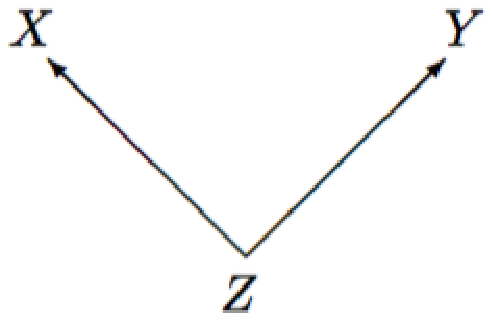
\includegraphics[width=3.70000cm]{xyzspurious.pdf}
\caption{\label{fig:f-xyzspurious} A graphical representation of a spurious
association between \(X\) and \(Y\), explained by dependence on a common
cause \(Z\).}
\end{figure}

To illustrate a spurious association with a silly but memorable teaching
example, suppose that we examine a sample of house fires in London, and
record the number of fire engines sent to each incident (\(X\)) and the
amount of damage caused by the fire (\(Y\)). There will be a strong
association between \(X\) and \(Y\), with large numbers of fire engines
associated with large amounts of damage. It is also reasonably clear
that the number of fire engines is determined before the final extent of
damage. The first two conditions discussed above are thus satisfied. We
would, however, be unlikely to infer from this that the relationship is
causal and conclude that we should try to reduce the cost of fires by
dispatching fewer fire engines to them. This is because the association
between the number of fire engines and the amount of damages is due to
both of them being influenced by the size of the fire (\(Z\)). Here this
is of course obvious, but in most real research questions possible
spurious associations are less easy to spot.

How can we then rule out spurious associations due to some background
variables \(Z\)? The usual approach is to try to remove the association
between \(X\) and \(Z\). This means in effect setting up comparisons
between units which have different values of \(X\) but the same or
similar values of \(Z\). Any differences in \(Y\) can then more
confidently be attributed to \(X\), because they cannot be due to
differences in \(Z\). This approach is known as \textbf{controlling} for
other variables \(Z\) in examining the association between \(X\) and
\(Y\).

The most powerful way of controlling for background variables is to
conduct a \textbf{randomized experiment}, where the values of the
explanatory variable \(X\) can be set by the researcher, and are
assigned at random to the units in the study. For instance, of the
examples considered in Chapters \ref{c-probs} and \ref{c-means},
Examples 5.3, 5.4 and 7.3 are randomized experiments, each with an
intervention variable \(X\) with two possible values (placebo or real
vaccine, one of two forms of a survey question, and police officer
wearing or not wearing sunglasses, respectively). The randomization
assures that units with different values of \(X\) are on average similar
in \emph{all} variables \(Z\) which precede \(X\) and \(Y\), thus ruling
out the possibility of spurious associations due to such variables.

Randomized experiments are for practical or ethical reasons infeasible
in many contexts, especially in the social sciences. We may then resort
to other, less powerful research designs which help to control for some
background variables. This, however, is usually only partially
successful, so we may also need methods of control applied at the
analysis stage of the research process. This is known as
\textbf{statistical control}. The aim of statistical control is to
estimate and test associations between \(X\) and \(Y\) while effectively
holding the values of some other variables \(Z\) constant in the
analysis. When the response variable is continuous, the most common way
of doing this is the method of multiple linear regression which is
described in the next section. When all the variables are categorical,
one simple way of achieving the control is analysis of multiway
contingency tables, which is described in Chapter \ref{c-3waytables}.

\section{Multiple linear regression models}\label{s-regression-multiple}

\subsection{Introduction}\label{ss-regression-multiple-intro}

Simple linear regression becomes multiple linear regression when more
than one explanatory variable is included in the model. How this is done
is explained in Section \ref{ss-regression-multiple-def} below. The
definition of the model builds directly on that of the simple linear
model, and most of the elements of the multiple model are either
unchanged or minimally modified from the simple one. As a result, we can
in Section \ref{ss-regression-multiple-unchanged} cover much of the
multiple linear model simply by referring back to the descriptions in
Section \ref{s-regression-simple}. One aspect of the model is, however,
conceptually expanded when there are multiple explanatory variables, and
requires a careful discussion. This is the meaning of the regression
coefficients of the explanatory variables. The interpretation of and
inference for these parameters are discussed in Section
\ref{ss-regression-multiple-beta}. The crucial part of this
interpretation, and the main motivation for considering multiple
regression models, is that it is one way of implementing the ideas of
statistical control in analyses for continuous response variables.

The concepts are be illustrated with a further example from the Global
Civil Society data set. The response variable will still be the Infant
mortality rate of a country, and there will be three explanatory
variables: School enrolment, Control of corruption and Income inequality
as measured by the Gini index (see Example 8.1). Results for this model
are shown in Table \ref{tab:t-imr-m2}, to which we will refer throughout
this section. The table is also an example of the kind of format in
which results of regression models are typically reported. Presenting
raw computer output such as that in Figure \ref{fig:f-spss-linreg} is
normally not appropriate in formal research reports.

\begin{longtable}[]{@{}lrrrrc@{}}
\caption{\label{tab:t-imr-m2} Response variable: Infant Mortality Rate (\%).
Results for a linear regression model for Infant mortality rate given
three explanatory variables in the Global Civil Society data.
\(\hat{\sigma}=2.23\); \(R^{2}=0.692\); \(n=111\);
\(df=107\)}\tabularnewline
\toprule
\begin{minipage}[t]{0.45\columnwidth}\raggedright\strut
Explanatory variable\strut
\end{minipage} & \begin{minipage}[t]{0.08\columnwidth}\raggedleft\strut
Coefficient\strut
\end{minipage} & \begin{minipage}[t]{0.06\columnwidth}\raggedleft\strut
Standard error\strut
\end{minipage} & \begin{minipage}[t]{0.05\columnwidth}\raggedleft\strut
\(t\)\strut
\end{minipage} & \begin{minipage}[t]{0.07\columnwidth}\raggedleft\strut
\(P\)-value\strut
\end{minipage} & \begin{minipage}[t]{0.11\columnwidth}\centering\strut
95 \% Confidence interval\strut
\end{minipage}\tabularnewline
\begin{minipage}[t]{0.45\columnwidth}\raggedright\strut
Constant\strut
\end{minipage} & \begin{minipage}[t]{0.08\columnwidth}\raggedleft\strut
16.40\strut
\end{minipage} & \begin{minipage}[t]{0.06\columnwidth}\raggedleft\strut
\strut
\end{minipage} & \begin{minipage}[t]{0.05\columnwidth}\raggedleft\strut
\strut
\end{minipage} & \begin{minipage}[t]{0.07\columnwidth}\raggedleft\strut
\strut
\end{minipage} & \begin{minipage}[t]{0.11\columnwidth}\centering\strut
\strut
\end{minipage}\tabularnewline
\begin{minipage}[t]{0.45\columnwidth}\raggedright\strut
School enrolment (\%)\strut
\end{minipage} & \begin{minipage}[t]{0.08\columnwidth}\raggedleft\strut
-0.139\strut
\end{minipage} & \begin{minipage}[t]{0.06\columnwidth}\raggedleft\strut
0.014\strut
\end{minipage} & \begin{minipage}[t]{0.05\columnwidth}\raggedleft\strut
-9.87\strut
\end{minipage} & \begin{minipage}[t]{0.07\columnwidth}\raggedleft\strut
\(<0.001\)\strut
\end{minipage} & \begin{minipage}[t]{0.11\columnwidth}\centering\strut
(-0.167; -0.111 )\strut
\end{minipage}\tabularnewline
\begin{minipage}[t]{0.45\columnwidth}\raggedright\strut
Control of corruption\strut
\end{minipage} & \begin{minipage}[t]{0.08\columnwidth}\raggedleft\strut
-0.046\strut
\end{minipage} & \begin{minipage}[t]{0.06\columnwidth}\raggedleft\strut
0.008\strut
\end{minipage} & \begin{minipage}[t]{0.05\columnwidth}\raggedleft\strut
-5.53\strut
\end{minipage} & \begin{minipage}[t]{0.07\columnwidth}\raggedleft\strut
\(<0.001\)\strut
\end{minipage} & \begin{minipage}[t]{0.11\columnwidth}\centering\strut
(-0.062; -0.029)\strut
\end{minipage}\tabularnewline
\begin{minipage}[t]{0.45\columnwidth}\raggedright\strut
Income inequality\strut
\end{minipage} & \begin{minipage}[t]{0.08\columnwidth}\raggedleft\strut
0.055\strut
\end{minipage} & \begin{minipage}[t]{0.06\columnwidth}\raggedleft\strut
0.022\strut
\end{minipage} & \begin{minipage}[t]{0.05\columnwidth}\raggedleft\strut
2.50\strut
\end{minipage} & \begin{minipage}[t]{0.07\columnwidth}\raggedleft\strut
0.014\strut
\end{minipage} & \begin{minipage}[t]{0.11\columnwidth}\centering\strut
(0.011; 0.098)\strut
\end{minipage}\tabularnewline
\bottomrule
\end{longtable}

\subsection{Definition of the model}\label{ss-regression-multiple-def}

Having multiple explanatory variables requires a slight extension of
notation. Let us denote the number of explanatory variables in the model
by \(k\); in our example \(k=3\). Individual explanatory variables are
then denoted with subscripts as \(X_{1}\), \(X_{2}\), \ldots{},
\(X_{k}\), in the example for instance as \(X_{1}=\) School enrolment,
\(X_{2}=\) Control of corruption and \(X_{3}=\) Income inequality.
Observations for individual units \(i\) (with values \(i=1,2,\dots,n\))
in the sample are indicated by a further subscript, so that
\(X_{1i}, X_{2i}, \dots, X_{ki}\) denote the observed values of the
\(k\) explanatory variables for unit \(i\).

The multiple linear regression model is essentially the same as the
simple linear model. The values \(Y_{i}\) of the response variable in
the sample are again assumed to be statistically independent, and each
of them is regarded as an observation sampled from a normal distribution
with mean \(\mu_{i}\) and variance \(\sigma^{2}\). The crucial change is
that the expected values \(\mu_{i}\) now depend on the multiple
explanatory variables through

\begin{equation}\mu_{i} = \alpha +\beta_{1}X_{1i}+\beta_{2}X_{2i}+\dots+\beta_{k}X_{ki}
\label{eq:mu-multiple}\end{equation}

where the coefficients \(\beta_{1}, \beta_{2}, \dots, \beta_{k}\) of
individual explanatory variables are now also identified with
subscripts. As in (\ref{eq:slinmodel}) for the simple linear model, the
multiple model can also be expressed in the concise form

\begin{equation}Y_{i} = \alpha
+\beta_{1}X_{1i}+\beta_{2}X_{2i}+\dots+\beta_{k}X_{ki}+\epsilon_{i}
\label{eq:mlinmodel}\end{equation}

where the error term (population residual) \(\epsilon_{i}\) is normally
distributed with mean 0 and variance \(\sigma^{2}\).

The expected value of \(Y\) as defined in (\ref{eq:mu-multiple}) is a
linear function of \(X_{1}, X_{2}, \dots, X_{k}\). If there are two
explanatory variables (\(k=2\)), \(\mu\) is described by a flat
\emph{plane} as \(X_{1}\) and \(X_{2}\) take different values (think of
a flat sheet of paper, at an angle and extended indefinitely in all
directions, cutting across a room in the air). A plane is the
two-dimensional generalisation of a one-dimensional straight line. The
actual observations of \(Y_{i}\) now correspond to points in a
three-dimensional space, and they are generally not on the regression
plane (think of them as a swarm of bees in the air, some perhaps sitting
on that sheet of paper but most hovering above or below it). When \(k\)
is larger than 2, the regression surface is a higher-dimensional linear
object known as a hyperplane. This is impossible to visualise in our
three-dimensional world, but mathematically the idea of the model
remains unchanged. In each case, the observed values of \(Y\) exist in a
yet higher dimension, so they cannot in general be predicted exactly
even with multiple explanatory variables. A regression plane defined by
several \(X\)-variables does nevertheless allow for more flexibility for
\(\mu_{i}\) than a straight line, so it is in general possible to
predict \(Y_{i}\) more accurately with a multiple regression model than
a simple one. This, however, is not usually the only or main criterion
for selecting a good regression model, for reasons discussed in Section
\ref{ss-regression-multiple-beta} below.

\subsection{Unchanged elements from simple linear
models}\label{ss-regression-multiple-unchanged}

As mentioned at the beginning of this section, most elements of the
multiple linear regression model are the same or very similar as for the
simple model, and require little further explanation:

\begin{itemize}
\item
  The \textbf{constant term} (intercept) \(\alpha\) is interpreted as
  the expected value of \(Y\) when all of the explanatory variables have
  the value 0. This can be seen by setting
  \(X_{1i}, X_{2i}, \dots, X_{ki}\) all to 0 in (\ref{eq:mu-multiple}).
  As before, \(\alpha\) is rarely of any substantive interest. In the
  example in Table \ref{tab:t-imr-m2}, the estimated value of \(\alpha\)
  is 16.40.
\item
  The \textbf{residual standard deviation} \(\sigma\) is the standard
  deviation of the conditional distribution of \(Y\) given the values of
  all of \(X_{1}, X_{2}, \dots, X_{k}\). It thus describes the magnitude
  of the variability of \(Y\) around the regression plane. The model
  assumes that \(\sigma\) is the same at all values of the explanatory
  variables. In Table \ref{tab:t-imr-m2}, the estimate of \(\sigma\) is
  2.23.
\item
  \textbf{Estimates of the regression coefficients} are here denoted
  with hats as \(\hat{\alpha}\) and
  \(\hat{\beta}_{1}, \hat{\beta}_{2}, \dots, \hat{\beta}_{k}\), and
  fitted (predicted) values for \(Y_{i}\) are given by

  \begin{equation}\hat{Y}_{i}=\hat{\alpha}+\hat{\beta}_{1}X_{1i}+\hat{\beta}_{2}X_{2i}+\dots+
  \hat{\beta}_{k}X_{ki}.
  \label{eq:Yhat}\end{equation}

  The estimated regression coefficients are again obtained with the
  method of \textbf{least squares} by finding the values for
  \(\hat{\alpha}, \hat{\beta}_{1}, \hat{\beta}_{2}, \dots, \hat{\beta}_{k}\)
  which make the error sum of squares
  \(SSE=\sum (Y_{i}-\hat{Y}_{i})^{2}\) as small as possible. This is
  both mathematically and intuitively the same exercise as least squares
  estimation for a simple linear model, except with more dimensions:
  here we are finding the best-fitting hyperplane through a
  high-dimensional cloud of points rather than the best-fitting straight
  line through a two-dimensional scatterplot.

  With more than one explanatory variable, the computational formulas
  for the estimates become difficult to write down\footnote{At least
    until we adopt extended, so-called matrix notation. In this, the
    least squares estimates are expressible simply as
    \(\hat{\boldsymbol{\beta}}= (\mathbf{X}'\mathbf{X})^{-1}(\mathbf{X}'\mathbf{Y})\).}
  and essentially impossible to calculate by hand. This is not a problem
  in practice, as they are easily computed by statistical software such
  as SPSS. In Table \ref{tab:t-imr-m2}, the least squares estimates of
  the regression coefficients are shown in the ``Coefficient'' column.
  Each row of the table gives the coefficient for one explanatory
  variable, identified in the first column. A similar format is adopted
  in SPSS output, where the ``\textbf{Coefficients}'' table looks very
  similar to the main part of Table \ref{tab:t-imr-m2}. The arrangement
  of other parts of SPSS output for multiple linear regression is
  essentially unchanged from the format shown in Figure
  \ref{fig:f-spss-linreg}.
\item
  Predicted values for \(Y\) can be calculated from (\ref{eq:Yhat}) for
  any set of values of the explanatory variables (whether those observed
  in the data or not, as long as extrapolation outside their observed
  ranges is avoided). This is often very useful for illustrating the
  implications of a fitted model. For example, Table \ref{tab:t-imrvars}
  shows that the sample averages of the explanatory variables in Table
  \ref{tab:t-imr-m2} are approximately 86 for School enrolment
  (\(X-{1}\)), 50 for Control of corruption (\(X_{2}\)) and 40 for
  Income inequality (\(X_{3}\)). The predicted IMR for a hypothetical
  ``average'' country with all these values would be
  \[\hat{Y}=16.4-0.139\times 86-0.046\times 50+0.055\times 40=4.35\]
  using the estimated intercept \(\hat{\alpha}=16.4\), and the estimated
  regression coefficients \(\hat{\beta}_{1}=-0.139\),
  \(\hat{\beta}_{2}=-0.046\) and \(\hat{\beta}_{3}=0.055\) for
  \(X_{1}\), \(X_{2}\) and \(X_{3}\). For further illustration, we might
  compare this to other predicted values calculated for, say, different
  combinations of large and/or small values of the explanatory
  variables.
\item
  The estimated residual standard error \(\hat{\sigma}\) is again
  calculated from (\ref{eq:sigma-linreg}), using the appropriate value
  of \(k\). Here \(n=111\) and \(k=3\), and so the degrees of freedom
  are \(df=n-(k+1)=n-4=107\). The estimate is \(\hat{\sigma}=2.23\).
\item
  The explanation of the coefficient of determination \(R^{2}\) is
  entirely unchanged from the one given under ``Coefficient of
  determination (\(R^{2}\))'' in Section \ref{ss-regression-simple-est}.
  It is still calculated with the formula (\ref{eq:R2}), and its
  interpretation is also the same. The \(R^{2}\) statistic thus
  describes the proportion of the sample variation in \(Y\) explained by
  the regression model, i.e.~by the variation in the explanatory
  variables. Similarly, the multiple correlation coefficient
  \(R=\sqrt{R^{2}}\) is again the correlation between the observed
  \(Y_{i}\) and the fitted values \(\hat{Y}_{i}\). In our example,
  \(R^{2}=0.692\) (and \(R=\sqrt{0.692}=0.832\)), i.e.~about 69.2\% of
  the observed variation in IMR between countries is explained by the
  variation in levels of School enrolment, Control of corruption and
  Income inequality between them. Compared to the \(R^{2}=0.567\) for
  the simple regression model in Figure \ref{fig:f-spss-linreg}, adding
  the two new explanatory variables has increased \(R^{2}\) by 12.5
  percentage points, which seems like a reasonably large increase.
\end{itemize}

\subsection{Interpretation and inference for the regression
coefficients}\label{ss-regression-multiple-beta}

\subsubsection*{Interpretation}\label{interpretation}
\addcontentsline{toc}{subsubsection}{Interpretation}

The concept of statistical control was outlined in Section
\ref{s-regression-causality} above. In essence, its idea is to examine
the association between a response variable and a particular explanatory
variable, while holding all other explanatory variables at constant
values. This is useful for assessing claims about causal effects, but
also more broadly whenever we want to analyse associations free of the
confounding effects of other variables.

When all of the variables were categorical, statistical control could be
carried out obviously and transparently by considering partial tables,
where the control variables are literally held constant. This is not
possible when some of the control variables are continuous, because they
then have too many different values for it to be feasible to consider
each one separately. Instead, statistical control is implemented with
the help of a multiple regression model, and interpreted in terms of the
regression coefficients.

Consider, for example, a linear regression model with three explanatory
variables \(X_{1}\), \(X_{2}\) and \(X_{3}\). This specifies the
expected value of \(Y\) as

\begin{equation}\mu=\alpha+\beta_{1}X_{1}+\beta_{2}X_{2}+\beta_{3}X_{3}
\label{eq:mu1}\end{equation}

for any values of \(X_{1}\), \(X_{2}\) and \(X_{3}\). Suppose now that
we consider a second observation, which has the same values of \(X_{1}\)
and \(X_{2}\) as before, but the value of \(X_{3}\) larger by one unit,
i.e.~\(X_{3}+1\). The expected value of \(Y\) is now

\begin{equation}\mu=\alpha+\beta_{1}X_{1}+\beta_{2}X_{2}+\beta_{3}(X_{3}+1)=
\alpha+\beta_{1}X_{1}+\beta_{2}X_{2}+\beta_{3}X_{3}+\beta_{3}.
\label{eq:mu2}\end{equation}

Subtracting (\ref{eq:mu1}) from (\ref{eq:mu2}) leaves us with
\(\beta_{3}\). In other words, \(\beta_{3}\) is the change in expected
value of \(Y\) when \(X_{3}\) is increased by one unit, while keeping
the values of \(X_{1}\) and \(X_{2}\) unchanged. The same result would
obviously be obtained for \(X_{1}\) and \(X_{2}\), and for models with
any number of explanatory variables. Thus in general

\begin{itemize}
\tightlist
\item
  The regression coefficient of any explanatory variable in a multiple
  linear regression model shows the change in expected value of the
  response variable \(Y\) when that explanatory variable is increased by
  one unit, while holding all other explanatory variables constant.
\end{itemize}

When there is only one explanatory variable, the ``while
holding\ldots{}'' part is omitted and the interpretation becomes the one
for simple linear regression in Section \ref{ss-regression-simple-int}.

This interpretation of the regression coefficients is obtained by
``increasing by one unit'' and ``holding constant'' values of
explanatory variables by mathematical manipulations alone. It is thus
true within the model even when the values of the explanatory variables
are not and cannot actually be controlled and set at different values by
the researcher. This, however, also implies that this appealing
interpretation is a mathematical construction which does not
automatically correspond to reality. In short, the interpretation of the
regression coefficients is always mathematically true, but whether it is
also an approximately correct description of an association in the real
world depends on the appropriateness of the model for the data and study
at hand. In some studies it is indeed possible to manipulate at least
some explanatory variables, and corresponding regression models can then
help to draw reasonably strong conclusions about associations between
variables. Useful results can also be obtained in studies where no
variables are in our control (so-called \emph{observational studies}),
as long as the model is selected carefully. This requires, in
particular, that a linear model specification is adequate for the data,
and that no crucially important explanatory variables have been omitted
from the model.

In the IMR example, the estimated coefficients in Table
\ref{tab:t-imr-m2} are interpreted as follows:

\begin{itemize}
\item
  Holding levels of Control of corruption and Income inequality
  constant, increasing School enrolment by one percentage point
  decreases expected IMR by 0.139 percentage points.
\item
  Holding levels of School enrolment and Income inequality constant,
  increasing Control of corruption by one unit decreases expected IMR by
  0.046 percentage points.
\item
  Holding levels of School enrolment and Control of corruption constant,
  increasing Income inequality by one unit increases expected IMR by
  0.055 percentage points.
\end{itemize}

Instead of ``holding constant'', we often talk about ``controlling for''
other variables in such statements. As before, it may be more convenient
to express the interpretations in terms of other increments than one
unit (e.g.~ten units of the measure of Income inequality) by multiplying
the coefficient by the correponding value.

The association between the response variable \(Y\) and a particular
explanatory variable \(X\) described by the coefficient of \(X\) in a
multiple regression model is known as a \textbf{partial association}
between \(X\) and \(Y\), controlling for the other explanatory variables
in the model. This will often differ from the association estimated from
a simple regression model for \(Y\) given \(X\), because of the
correlations between the control variables and \(X\) and \(Y\). In the
infant mortality example, the estimated effect of School enrolment was
qualitatively unaffected by controlling for the other variables, and
decreased in magnitude from -0.179 to -0.139.

\subsubsection*{Inference}\label{inference}
\addcontentsline{toc}{subsubsection}{Inference}

Inference for the regression coefficients in a multiple linear model
differs from that for the simple model in interpretation but not in
execution. Let \(\hat{\beta}_{j}\) denote the estimated coefficient of
an explanatory variable \(X_{j}\) (where \(j\) may be any of
\(1,2,\dots,k\)), and let \(\hat{\text{se}}(\hat{\beta}_{j})\) denote
its estimated standard error. The standard errors cannot now be
calculated by hand, but they are routinely produced by computer packages
and displayed as in Table \ref{tab:t-imr-m2}. A \(t\)-test statistic for
the null hypothesis discussed below is given by

\begin{equation}t=\frac{\hat{\beta}_{j}}{\hat{\text{se}}(\hat{\beta}_{j})}.
\label{eq:tbeta-m}\end{equation}

This is identical in form to statistic (\ref{eq:tbeta}) for the simple
regression model. The corresponding null hypotheses are, however, subtly
but crucially different in the two cases. In a multiple model,
(\ref{eq:tbeta-m}) is a test statistic for the null hypothesis

\begin{equation}H_{0}:\; \beta_{j}=0, \text{other regression coefficients
are unrestricted}
\label{eq:H0beta-m}\end{equation}

against the alternative hypothesis
\[H_{a}:\; \beta_{j}\ne0, \text{other regression coefficients
are unrestricted}.\] Here the statement about ``unrestricted'' other
parameters implies that neither hypothesis makes any claims about the
values of other coefficients than \(\beta_{j}\), and these are allowed
to have any values. The null hypothesis is a claim about the association
between \(X_{j}\) and \(Y\) when the other explanatory variables are
already included in the model. In other words, (\ref{eq:tbeta-m}) tests
\[\begin{aligned}
H_{0}:& & \text{There is no partial association between }
X_{j} \text{ and } Y,\\
&&  \text{controlling for the other explanatory
variables.}\end{aligned}\]

The sampling distribution of (\ref{eq:tbeta-m}) when the null hypothesis
(\ref{eq:H0beta-m}) holds is a \(t\) distribution with \(n-(k+1)\)
degrees of freedom, where \(k\) is again the number of explanatory
variables in the model. The test statistic and its \(P\)-value from the
\(t_{n-(k+1)}\) distribution are shown in standard computer output, in a
form similar to Table \ref{tab:t-imr-m2}.

It is important to note two things about test results for multiple
regression models, such as those in Table \ref{tab:t-imr-m2}. First,
(\ref{eq:H0beta-m}) implies that if the null hypothesis is not rejected,
\(X_{j}\) is not associated with \(Y\), \emph{if} the other explanatory
variables are already included in the model. We would typically react to
this by removing \(X_{j}\) from the model, while keeping the other
variables in it. This is because of a general principle that models
should usually be as simple (\emph{parsimonious}) as possible, and not
include variables which have no partial effect on the response variable.
Second, the \(k\) tests and \(P\)-values actually refer to \(k\)
\emph{different} hypotheses of the form (\ref{eq:H0beta-m}), one for
each explanatory variable. This raises the question of what to do if,
say, tests for two variables have large \(P\)-values, suggesting that
either of them could be removed from the model. The appropriate reaction
is to remove one of the variables (perhaps the one with the larger
\(P\)-value) rather than both at once, and then see whether the other
still remains nonsignificant (if so, it can then also be removed). This
is part of the general area of \textbf{model selection}, principles and
practice of which are mostly beyond the scope of this course; some
further comments on it are given in Section \ref{s-regression-rest}.

In the example shown in Table \ref{tab:t-imr-m2}, the \(P\)-values are
small for the tests for all of the coefficients. Each of the three
explanatory variables thus has a significant effect on the response even
after controlling for the other two, so none of the variables should be
removed from the model.

A confidence interval with confidence level \(1-\alpha\) for any
\(\beta_{j}\) is given by

\begin{equation}\hat{\beta}_{j} \pm t_{\alpha/2}^{(n-(k+1))} \,
\hat{\text{se}}(\hat{\beta}_{j}).
\label{eq:cibeta-m}\end{equation}

This is identical in form and interpretation to the interval
(\ref{eq:cibeta}) for simple regression (except that the degrees of
freedom are now \(df=n-(k+1)\)), so no new issues arise. The confidence
intervals for the coefficients in our example (where \(df=n-4=107\) and
\(t_{0.025}^{(107)}=1.98\)) are shown in Table \ref{tab:t-imr-m2}.

\section{Including categorical explanatory
variables}\label{s-regression-dummies}

\subsection{Dummy variables}\label{ss-regression-dummies-def}

Our models for Infant mortality rate so far did not include some more
basic characteristics of the countries than school enrolment, corruption
and income inequality. In particular, it seems desirable to control for
the wealth of a country, which is likely to be correlated with both a
health outcome like infant mortality and the other measures of
development used as explanatory variables. We will do this by adding to
the model the income level of the country, classified in the Global
Civil Society Yearbook into three groups as Low, Middle or High income.
Here one reason for considering income as a categorical variable is
obviously to obtain an illustrative example for this section. However,
using a variable like income in a grouped form is also more generally
common practice. It also has the advantage that it is one way of dealing
with cases where the effects on \(Y\) of the corresponding continuous
explanatory variable may be nonlinear.

Summary statistics in Table \ref{tab:t-imrvars} show that income group
is associated with both IMR and the explanatory variables considered so
far: countries with higher income tend to have lower levels of infant
mortality, and higher school enrolment, less corruption and less income
inequality than lower-income countries. It thus seems that controlling
for income is potentially necessary, and may change the conclusions from
the model.

Trying to add income level to the model confronts us with a new problem:
how can a categorical explanatory variable like this be used in linear
regression? This question is not limited to the current example, but is
unavoidable in the social sciences. Even just the standard background
variables such as sex, marital status, education level, party
preference, employment status and region of residence considered in most
individual-level studies are mostly categorical. Similarly, most survey
data on attitudes and behaviour are collected in a categorical form, and
even variables such as age or income which are originally continuous are
often used in a grouped form. Categorical variables are thus ubiquitous
in the social sciences, and it is essential to be able to use them also
in regression models. How this is done is explained in this section,
again illustrated with the infant mortality example. Section
\ref{ss-regression-dummies-example} then describes a different example
for further illustration of the techniques.

The key to handling categorical explanatory variables is the use of
dummy variables. A \textbf{dummy variable} (or \textbf{indicator
variable}) is a variable with only two values, 0 and 1. Its value is 1
if a unit is in a particular category of a categorical variable, and 0
if it is not in that category. For example, we can define for each
country the variable \[D_{m}=\begin{cases}
1 & \text{if Income level is ``Middle''} \\
0 & \text{otherwise.}
\end{cases}\] This would typically be referred to as something like
``dummy for middle income level''. Note that the label \(D_{m}\) used
here has no special significance, and was chosen simply to make it easy
to remember. Dummy variables will be treated below as regular
explanatory variables, and we could denote them as \(X\)s just like all
the others. A dummy for high income level is defined similarly as
\[D_{h}=\begin{cases}
1 & \text{if Income level is ``High''} \\
0 & \text{otherwise.}
\end{cases}\] The two variables \(D_{m}\) and \(D_{h}\) are enough to
identify the income level of any country. If a country is in the
middle-income group, the two dummies have the values \(D_{m}=1\) and
\(D_{h}=0\) (as no country can be in two groups), and if it has high
income, the dummies are \(D_{m}=0\) and \(D_{h}=1\). For low-income
countries, both \(D_{m}=0\) and \(D_{h}=0\). There is thus no need to
define a dummy for low income, because this category is identified by
the two other dummies being both zero. The same is true in general: if a
categorical variable has \(K\) categories, only \(K-1\) dummy variables
are needed to identify the category of every unit. Note, in particular,
that \emph{dichotomous} variables with only two categories (\(K=2\)) are
fully identified by just one dummy variable. The category which is not
given a dummy of its own is known as the \textbf{reference category} or
\textbf{baseline category}. Any category can be the baseline, and this
is usually chosen in a way to make interpretation (discussed below)
convenient. The results of the model will be the same, whichever
baseline is used.

Categorical variables are used as explanatory variables in regression
models by including the dummy variables for them in the model. The
results for this in our example are shown in Table \ref{tab:t-imr-m3}.
This requires no changes in the definition or estimation of the model,
and the parameter estimates, standard errors and quantities for
statistical inference are obtained exactly as before even when some of
the explanatory variables are dummy variables. The only aspect which
requires some further explanation is the interpretation of the
coefficients of the dummy variables.

\begin{longtable}[]{@{}lrrrrc@{}}
\caption{\label{tab:t-imr-m3} Response variable: Infant Mortality Rate (\%).
Results for a linear regression model for Infant mortality rate in the
Global Civil Society data, given the three explanatory variables in
Table \ref{tab:t-imr-m2} and Income level in three groups.
\(\hat{\sigma}=2.01\); \(R^{2}=0.753\); \(n=111\);
\(df=105\).}\tabularnewline
\toprule
\begin{minipage}[t]{0.44\columnwidth}\raggedright\strut
Explanatory variable\strut
\end{minipage} & \begin{minipage}[t]{0.09\columnwidth}\raggedleft\strut
Coefficient\strut
\end{minipage} & \begin{minipage}[t]{0.05\columnwidth}\raggedleft\strut
Std.~ error\strut
\end{minipage} & \begin{minipage}[t]{0.06\columnwidth}\raggedleft\strut
\(t\)\strut
\end{minipage} & \begin{minipage}[t]{0.08\columnwidth}\raggedleft\strut
\(P\)-value\strut
\end{minipage} & \begin{minipage}[t]{0.10\columnwidth}\centering\strut
95 \% Conf.~ interval\strut
\end{minipage}\tabularnewline
\begin{minipage}[t]{0.44\columnwidth}\raggedright\strut
Constant\strut
\end{minipage} & \begin{minipage}[t]{0.09\columnwidth}\raggedleft\strut
12.00\strut
\end{minipage} & \begin{minipage}[t]{0.05\columnwidth}\raggedleft\strut
\strut
\end{minipage} & \begin{minipage}[t]{0.06\columnwidth}\raggedleft\strut
\strut
\end{minipage} & \begin{minipage}[t]{0.08\columnwidth}\raggedleft\strut
\strut
\end{minipage} & \begin{minipage}[t]{0.10\columnwidth}\centering\strut
\strut
\end{minipage}\tabularnewline
\begin{minipage}[t]{0.44\columnwidth}\raggedright\strut
School enrolment (\%)\strut
\end{minipage} & \begin{minipage}[t]{0.09\columnwidth}\raggedleft\strut
\(-0.091\)\strut
\end{minipage} & \begin{minipage}[t]{0.05\columnwidth}\raggedleft\strut
0.016\strut
\end{minipage} & \begin{minipage}[t]{0.06\columnwidth}\raggedleft\strut
\(-5.69\)\strut
\end{minipage} & \begin{minipage}[t]{0.08\columnwidth}\raggedleft\strut
\(<0.001\)\strut
\end{minipage} & \begin{minipage}[t]{0.10\columnwidth}\centering\strut
\((-0.123; -0.059)\)\strut
\end{minipage}\tabularnewline
\begin{minipage}[t]{0.44\columnwidth}\raggedright\strut
Control of corruption\strut
\end{minipage} & \begin{minipage}[t]{0.09\columnwidth}\raggedleft\strut
\(-0.020\)\strut
\end{minipage} & \begin{minipage}[t]{0.05\columnwidth}\raggedleft\strut
0.011\strut
\end{minipage} & \begin{minipage}[t]{0.06\columnwidth}\raggedleft\strut
\(-1.75\)\strut
\end{minipage} & \begin{minipage}[t]{0.08\columnwidth}\raggedleft\strut
\(0.083\)\strut
\end{minipage} & \begin{minipage}[t]{0.10\columnwidth}\centering\strut
\((-0.043; 0.003)\)\strut
\end{minipage}\tabularnewline
\begin{minipage}[t]{0.44\columnwidth}\raggedright\strut
Income inequality\strut
\end{minipage} & \begin{minipage}[t]{0.09\columnwidth}\raggedleft\strut
0.080\strut
\end{minipage} & \begin{minipage}[t]{0.05\columnwidth}\raggedleft\strut
0.021\strut
\end{minipage} & \begin{minipage}[t]{0.06\columnwidth}\raggedleft\strut
3.75\strut
\end{minipage} & \begin{minipage}[t]{0.08\columnwidth}\raggedleft\strut
\(<0.001\)\strut
\end{minipage} & \begin{minipage}[t]{0.10\columnwidth}\centering\strut
(0.038; 0.122)\strut
\end{minipage}\tabularnewline
\begin{minipage}[t]{0.44\columnwidth}\raggedright\strut
Income level (Reference group: Low)\strut
\end{minipage} & \begin{minipage}[t]{0.09\columnwidth}\raggedleft\strut
\strut
\end{minipage} & \begin{minipage}[t]{0.05\columnwidth}\raggedleft\strut
\strut
\end{minipage} & \begin{minipage}[t]{0.06\columnwidth}\raggedleft\strut
\strut
\end{minipage} & \begin{minipage}[t]{0.08\columnwidth}\raggedleft\strut
\strut
\end{minipage} & \begin{minipage}[t]{0.10\columnwidth}\centering\strut
\strut
\end{minipage}\tabularnewline
\begin{minipage}[t]{0.44\columnwidth}\raggedright\strut
Middle\strut
\end{minipage} & \begin{minipage}[t]{0.09\columnwidth}\raggedleft\strut
\(-3.210\)\strut
\end{minipage} & \begin{minipage}[t]{0.05\columnwidth}\raggedleft\strut
0.631\strut
\end{minipage} & \begin{minipage}[t]{0.06\columnwidth}\raggedleft\strut
\(-5.09\)\strut
\end{minipage} & \begin{minipage}[t]{0.08\columnwidth}\raggedleft\strut
\(<0.001\)\strut
\end{minipage} & \begin{minipage}[t]{0.10\columnwidth}\centering\strut
\((-4.461; -1.958)\)\strut
\end{minipage}\tabularnewline
\begin{minipage}[t]{0.44\columnwidth}\raggedright\strut
High\strut
\end{minipage} & \begin{minipage}[t]{0.09\columnwidth}\raggedleft\strut
\(-3.296\)\strut
\end{minipage} & \begin{minipage}[t]{0.05\columnwidth}\raggedleft\strut
1.039\strut
\end{minipage} & \begin{minipage}[t]{0.06\columnwidth}\raggedleft\strut
\(-3.17\)\strut
\end{minipage} & \begin{minipage}[t]{0.08\columnwidth}\raggedleft\strut
0.002\strut
\end{minipage} & \begin{minipage}[t]{0.10\columnwidth}\centering\strut
\((-5.357; -1.235)\)\strut
\end{minipage}\tabularnewline
\bottomrule
\end{longtable}

Recall that the regression coefficient of a continuous explanatory
variable \(X\) is the expected change in the response variable when
\(X\) is increased by one unit, holding all other explanatory variables
constant. Exactly the same interpretation works for dummy variables,
except that it is limited to the only one-unit increase possible for
them, i.e.~from 0 to 1. For example, consider two (hypothetical)
countries with values 0 and 1 for the dummy \(D_{m}\) for middle income,
but with the same values for the three continuous explanatory variables.
How about the other dummy variable \(D_{h}\), for high income? The
interpretation requires that this too is held constant in the
comparison. If this constant value was 1, it would not be possible for
\(D_{m}\) to be 1 because every country is in only one income group.
Thus the only value at which \(D_{h}\) can be held constant while
\(D_{m}\) is changed is 0, so that the comparison will be between a
country with \(D_{m}=1, \, D_{h}=0\) and one with
\(D_{m}=0,\, D_{h}=0\), both with the same values of the other
explanatory variables. In other words, the interpretation of the
coefficient of \(D_{m}\) refers to a comparison in expected value of
\(Y\) between a middle-income country and a country in the baseline
category of low income, controlling for the other explanatory variables.
The same applies to the coefficient of \(D_{h}\), and of dummy variables
in general:

\begin{itemize}
\tightlist
\item
  The coefficient of a dummy variable for a particular level of a
  categorical explanatory variable is interpreted as the
  \emph{difference} in the expected value of the response variable \(Y\)
  between a unit with that level of the categorical variable and a unit
  in the baseline category, holding all other explanatory variables
  constant.
\end{itemize}

Here the estimated coefficient of \(D_{m}\) is \(-3.21\). In other
words, comparing a middle-income country and a low-income country, both
with the same levels of School enrolment, Control of corruption and
Income inequality, the expected IMR is 3.21 percentage points lower in
the middle-income country than in the low-income one. Similarly, a
high-income country has an expected IMR 3.296 percentage points lower
than a low-income one, other things being equal. The expected difference
between the two non-reference levels is obtained as the difference of
their coefficients (or by making one of them the reference level, as
discussed below); here \(-3.296-(-3.210)=-0.086\), so a high-income
country has an expected IMR 0.086 percentage points lower than a
middle-income one, controlling for the other explanatory variables.

Predicted values are again obtained by substituting values for the
explanatory variables, including appropriate zeros and ones for the
dummy variables, into the estimated regression equation. For example,
the predicted IMR for a country with School enrolment of 86 \%, Control
of corruption score of 50 and Income inequality of 40 is
\[\begin{aligned}
\hat{Y}&=&12.0-0.091\times 86-0.020\times 50+0.080\times 40-3.210\times
0-3.296\times 0\\
&=&
6.37 \text{for a low-income country, and }\\
\hat{Y}&=&12.0-0.091\times 86-0.020\times 50+0.080\times 40-3.210\times
1-3.296\times 0\\
&=&
6.37-3.21=3.16 \text{for a middle-income country,}\end{aligned}\] with a
difference of 3.21, as expected. Note how the constant term 12.0 sets
the level for the baseline (low-income) group, and the coefficient
\(-3.21\) shows the change from that level when considering a
middle-income country instead. Note also that we should again avoid
unrealistic combinations of the variables in such predictions. For
example, the above values would not be appropriate for high-income
countries, because there are no such countries in these data with
Control of corruption as low as 50.

The choice of the reference category does not affect the fitted model,
and exactly the same results are obtained with any choice. For example,
if high income is used as the reference category instead, the
coefficients of the three continuous variables are unchanged from Table
\ref{tab:t-imr-m3}, and the coefficients of the dummy variables for low
and middle incomes are 3.296 and 0.086 respectively. The conclusions
from these are the same as above: controlling for the other explanatory
variables, the difference in expected IMR is 3.296 between low and
high-income, 0.086 between middle and high-income and
\(3.296-0.086=3.210\) between low and middle-income countries. Because
the choice is arbitrary, the baseline level should be selected in
whichever way is most convenient for stating the interpretation. If the
categorical variable is ordinal (as it is here), it makes most sense for
the baseline to be the first or last category. In other ways the
dummy-variable treatment makes no distinction between nominal and
ordinal categorical variables. Both are treated effectively as nominal
in fitting the model, and information on any ordering of the categories
is ignored.

Significance tests and confidence intervals are obtained for
coefficients of dummy variables exactly as for any regression
coefficients. Since the coefficient is in this case interpreted as an
expected difference between a level of a categorical variable and the
reference level, the null hypothesis of a zero coefficient is the
hypothesis that there is no such difference. For example, Table
\ref{tab:t-imr-m3} shows that the coefficients of both the middle income
and high income dummies are clearly significantly different from zero.
This shows that, controlling for the other explanatory variables,
expected infant mortality for both middle and high-income countries is
different from that in low-income countries. The 95\% confidence
intervals in Table \ref{tab:t-imr-m3} are intervals for this difference.

On the other hand, the coefficients of the two higher groups are very
similar, which suggests that they may not be different from each other.
This can be confirmed by fitting the same model with high income as the
reference level, including dummies for low and middle groups. In this
model (not shown here), the coefficient of the middle income dummy
corresponds to the difference of the Middle and High groups. Its
\(P\)-value is 0.907 and 95\% confidence interval \((-1.37; 1.54)\), so
the difference is clearly not significant. This suggests that we could
simplify the model further by combining the two higher groups and
considering only two income groups, low vs.~middle/high.

In cases like this where a categorical explanatory variable has more
than two categories, \(t\)-tests of individual coefficients are tests of
hypotheses about no differences between individual categories, not the
hypothesis that the variable has no effect overall. This is the
hypothesis that the coefficients of the dummies for \emph{all} of the
categories are zero. This requires a slightly different test, which will
not be considered here. In our example the low income category is so
obviously different from the other two that it is clear that the
hypothesis of no overall income effect would be rejected.

The main reason for including income group in the example was not to
study income effects themselves (it is after all not all that surprising
that infant mortality is highest in poor countries), but to control for
them when examining partial associations between IMR and the other
explanatory variables. These describe the estimated effects of these
continuous variables when comparing countries with similar income
levels. Comparing the results in Tables \ref{tab:t-imr-m2} and
\ref{tab:t-imr-m3}, it can be seen that the effect of School enrolment
remains significant and negative (with higher enrolment associated with
lower mortality), although its magnitude decreases somewhat after
controlling for income group. Some but not all of its estimated effect
in the first model is thus explained away by the fact that income is
associated with both primary school enrolment and infant mortality, with
richer countries having both higher enrolment and lower mortality.

The effect of Income inequality also remains significant in the larger
model, even with a slightly increased coefficient. Countries with larger
income inequality tend to have higher levels of infant mortality, even
when we compare countries with similar levels of income. The effect of
Control of corruption, on the other hand, is no longer significant in
Table \ref{tab:t-imr-m3}. This variable is strongly associated with
income (as seen in Table \ref{tab:t-imrvars}), with the more corrupt
countries typically being poor. Controlling for income, however, level
of corruption appears to have little further effect on infant mortality.
This also suggests that we might simplify the model by omitting the
corruption variable.

One final remark on dummy variables establishes a connection to the
techniques discussed in Chapter \ref{c-means}. There we described
statistical inference for comparisons of the population means of a
continuous response variable \(Y\) between two groups, denoted 1 and 2.
Suppose now that we fit a simple linear regression model for \(Y\), with
a dummy variable for group 2 as the only explanatory variable. This
gives exactly the same results as the two-sample \(t\)-tests and
confidence intervals (under the assumption of equal variances in the
groups) in Section \ref{s-means-inference}. Related to the notation of
that section, the coefficients from the model are
\(\hat{\alpha}=\bar{Y}_{1}\), \(\hat{\beta}=\bar{Y}_{2}-\bar{Y}_{1}\),
and \(\hat{\sigma}\) from (\ref{eq:sigma-linreg}) is equal to (see
equation 11 in Section \ref{ss-means-inference-test}). Similarly, the
standard error (\ref{eq:sebeta}) is the same as
\(\hat{\sigma}_{\hat{\Delta}}\) in the standard error equation in
Section \ref{ss-means-inference-test}, and the test statistic
(\ref{eq:tbeta}) and confidence interval (\ref{eq:cibeta}) are identical
with the t-test statistic in Section \ref{ss-means-inference-test} and
the \(t\) distribution version of the equation in Section
\ref{ss-means-inference-ci} respectively.

The connection between linear regression and the two-sample \(t\)-test
is an illustration of how statistical methods are not a series of
separate tricks for different situations, but a set of connected
procedures unified by common principles. Whenever possible, methods for
more complex problems have been created by extending those for simpler
ones, and simple analyses are in turn special cases of more general
ones. Although these connections are unfortunately often somewhat
obscured by changes in language and notation, trying to understand them
is very useful for effective learning of statistics.

\subsection{A second example}\label{ss-regression-dummies-example}

Because the analysis of the models for infant mortality was presented
piecemeal to accompany the introduction of different elements of linear
regression, an overall picture of that example may have been difficult
to discern. This section describes a different analysis in a more
concise manner. It is particularly an illustration of the use of dummy
variables, as most of the explanatory variables are categorical. The
example concerns the relationship between minimum wage and employment,
and uses data originally collected and analysed by David Card and Alan
Krueger.\footnote{Card, D.~and Krueger, A.~B.~(1994). Minimum wages and
  employment: A case study of the fast-food industry in New Jersey and
  Pennsylvania. \emph{The American Economic Review} \textbf{84},
  772--793.} Most of the choices of analyses and variables considered
here are based on those of Card and Krueger. Their article should be
consulted for discussion and more detailed analyses.

A minimum wage of \$5.05 per hour came into effect in the U.S.~state of
New Jersey on April 1 1992. This represented an increase from the
previous, federally mandated minimum wage of \$4.25 per hour.
Conventional economic theory predicts that employers will react to such
an increase by cutting their work force. Here the research hypothesis is
thus that employment will be reduced among businesses affected by the
new minimum wage. This can be addressed using suitable data, examining a
statistical hypothesis of no association between measures of minimum
wage increase and change of employment, controlling for other relevant
explanatory variables.

Card and Krueger collected data for 410 fast food restaurants at two
times, about one month before and eight months after the mininum wage
increase came into effect in New Jersey. Only the 368 restaurants with
known values of all the variables used in the analyses are included
here. Of them, 268 were in New Jersey and had starting wages below
\$5.05 at the time of the first interview, so that these had to be
increased to meet the new minimum wage. The remaining 100 restaurants
provide a control group which was not affected by the change: 75 of them
were in neighbouring eastern Pennsylvania where the minimum wage
remained at \$4.25, and 25 were in New Jersey but had starting wages of
at least \$5.05 even before the increase. The theoretical prediction is
that the control group should experience a smaller negative employment
change than the restaurants affected by the wage increase,
i.e.~employment in the control restaurants should not decrease or at
least decrease less than in the affected restaurants. Card and Krueger
argue that fast food restaurants provide a good population for examining
the research question, because they employ many low-wage workers,
generally comply with minimum wage legislation, do not receive tips
which would complicate wage calculations, and are relatively easy to
sample and interview.

The response variable considered here is the change between the two
interviews in full-time equivalent employment at the restaurant, defined
as the number of full-time workers (including managers) plus half the
number of part-time workers. This will be called ``Employment change''
below. We consider two variables which indicate how the restaurant was
affected by the minimum wage increase. The first is simply a dummy
variable which is 1 for those New Jersey restaurants where wages needed
to be raised because of the increase, and 0 for the other restaurants.
These will be referred to as ``Affected'' and ``Unaffected'' restaurants
respectively. The second variable is also 0 for the unaffected
restaurants; for the affected ones, it is the proportion by which their
previous starting wage had to be increased to meet the new minimum wage.
For example, if the previous starting wage was the old minimum of
\$4.25, this ``Wage gap'' is \((5.05-4.25)/4.25=0.188\). Finally, we
will also use information on the chain the restaurant belongs to (Burger
King, Roy Rogers, Wendy's or KFC) and whether it is owned by the parent
company or the franchisee. These will be included in the analyses as
partial control for other factors affecting the labour market, which
might have had a differential impact on different types of restaurants
over the study period. Summary statistics for the variables are shown in
Table \ref{tab:t-fastfood-descr}.

\begin{longtable}[]{@{}lrrrcc@{}}
\caption{\label{tab:t-fastfood-descr} Summary statistics for the variables
considered in the minimum wage example of Section
\ref{ss-regression-dummies-example}. Mean employment change: Among
unaffected restaurants: \(-2.93\); Among affected restaurants:
\(+0.68\).}\tabularnewline
\toprule
\begin{minipage}[t]{0.26\columnwidth}\raggedright\strut
\strut
\end{minipage} & \begin{minipage}[t]{0.04\columnwidth}\raggedleft\strut
\strut
\end{minipage} & \begin{minipage}[t]{0.05\columnwidth}\raggedleft\strut
\strut
\end{minipage} & \begin{minipage}[t]{0.29\columnwidth}\raggedleft\strut
Minimum\strut
\end{minipage} & \begin{minipage}[t]{0.10\columnwidth}\centering\strut
wage variable\strut
\end{minipage} & \begin{minipage}[t]{0.08\columnwidth}\centering\strut
\strut
\end{minipage}\tabularnewline
\begin{minipage}[t]{0.26\columnwidth}\raggedright\strut
Group\strut
\end{minipage} & \begin{minipage}[t]{0.04\columnwidth}\raggedleft\strut
\%\strut
\end{minipage} & \begin{minipage}[t]{0.05\columnwidth}\raggedleft\strut
\((n)\)\strut
\end{minipage} & \begin{minipage}[t]{0.29\columnwidth}\raggedleft\strut
Affected \% (\(n\))\strut
\end{minipage} & \begin{minipage}[t]{0.10\columnwidth}\centering\strut
Wage gap (mean for affected restaurants)\strut
\end{minipage} & \begin{minipage}[t]{0.08\columnwidth}\centering\strut
Response variable: Employment change (mean)\strut
\end{minipage}\tabularnewline
\begin{minipage}[t]{0.26\columnwidth}\raggedright\strut
Overall\strut
\end{minipage} & \begin{minipage}[t]{0.04\columnwidth}\raggedleft\strut
100\strut
\end{minipage} & \begin{minipage}[t]{0.05\columnwidth}\raggedleft\strut
(368)\strut
\end{minipage} & \begin{minipage}[t]{0.29\columnwidth}\raggedleft\strut
72.8 (268)\strut
\end{minipage} & \begin{minipage}[t]{0.10\columnwidth}\centering\strut
0.115\strut
\end{minipage} & \begin{minipage}[t]{0.08\columnwidth}\centering\strut
\(-0.30\)\strut
\end{minipage}\tabularnewline
\begin{minipage}[t]{0.26\columnwidth}\raggedright\strut
Ownership\strut
\end{minipage} & \begin{minipage}[t]{0.04\columnwidth}\raggedleft\strut
\strut
\end{minipage} & \begin{minipage}[t]{0.05\columnwidth}\raggedleft\strut
\strut
\end{minipage} & \begin{minipage}[t]{0.29\columnwidth}\raggedleft\strut
\strut
\end{minipage} & \begin{minipage}[t]{0.10\columnwidth}\centering\strut
\strut
\end{minipage} & \begin{minipage}[t]{0.08\columnwidth}\centering\strut
\strut
\end{minipage}\tabularnewline
\begin{minipage}[t]{0.26\columnwidth}\raggedright\strut
Franchisee\strut
\end{minipage} & \begin{minipage}[t]{0.04\columnwidth}\raggedleft\strut
64.7\strut
\end{minipage} & \begin{minipage}[t]{0.05\columnwidth}\raggedleft\strut
(238)\strut
\end{minipage} & \begin{minipage}[t]{0.29\columnwidth}\raggedleft\strut
71.8 (171)\strut
\end{minipage} & \begin{minipage}[t]{0.10\columnwidth}\centering\strut
0.122\strut
\end{minipage} & \begin{minipage}[t]{0.08\columnwidth}\centering\strut
\(-0.17\)\strut
\end{minipage}\tabularnewline
\begin{minipage}[t]{0.26\columnwidth}\raggedright\strut
Company\strut
\end{minipage} & \begin{minipage}[t]{0.04\columnwidth}\raggedleft\strut
35.3\strut
\end{minipage} & \begin{minipage}[t]{0.05\columnwidth}\raggedleft\strut
(130)\strut
\end{minipage} & \begin{minipage}[t]{0.29\columnwidth}\raggedleft\strut
74.6 (97)\strut
\end{minipage} & \begin{minipage}[t]{0.10\columnwidth}\centering\strut
0.103\strut
\end{minipage} & \begin{minipage}[t]{0.08\columnwidth}\centering\strut
\(-0.52\)\strut
\end{minipage}\tabularnewline
\begin{minipage}[t]{0.26\columnwidth}\raggedright\strut
Chain\strut
\end{minipage} & \begin{minipage}[t]{0.04\columnwidth}\raggedleft\strut
\strut
\end{minipage} & \begin{minipage}[t]{0.05\columnwidth}\raggedleft\strut
\strut
\end{minipage} & \begin{minipage}[t]{0.29\columnwidth}\raggedleft\strut
\strut
\end{minipage} & \begin{minipage}[t]{0.10\columnwidth}\centering\strut
\strut
\end{minipage} & \begin{minipage}[t]{0.08\columnwidth}\centering\strut
\strut
\end{minipage}\tabularnewline
\begin{minipage}[t]{0.26\columnwidth}\raggedright\strut
Burger King\strut
\end{minipage} & \begin{minipage}[t]{0.04\columnwidth}\raggedleft\strut
41.0\strut
\end{minipage} & \begin{minipage}[t]{0.05\columnwidth}\raggedleft\strut
(151)\strut
\end{minipage} & \begin{minipage}[t]{0.29\columnwidth}\raggedleft\strut
73.5 (111)\strut
\end{minipage} & \begin{minipage}[t]{0.10\columnwidth}\centering\strut
0.129\strut
\end{minipage} & \begin{minipage}[t]{0.08\columnwidth}\centering\strut
\(+0.02\)\strut
\end{minipage}\tabularnewline
\begin{minipage}[t]{0.26\columnwidth}\raggedright\strut
Roy Rogers\strut
\end{minipage} & \begin{minipage}[t]{0.04\columnwidth}\raggedleft\strut
24.7\strut
\end{minipage} & \begin{minipage}[t]{0.05\columnwidth}\raggedleft\strut
(91)\strut
\end{minipage} & \begin{minipage}[t]{0.29\columnwidth}\raggedleft\strut
72.5 (66)\strut
\end{minipage} & \begin{minipage}[t]{0.10\columnwidth}\centering\strut
0.104\strut
\end{minipage} & \begin{minipage}[t]{0.08\columnwidth}\centering\strut
\(-1.89\)\strut
\end{minipage}\tabularnewline
\begin{minipage}[t]{0.26\columnwidth}\raggedright\strut
Wendy's\strut
\end{minipage} & \begin{minipage}[t]{0.04\columnwidth}\raggedleft\strut
13.0\strut
\end{minipage} & \begin{minipage}[t]{0.05\columnwidth}\raggedleft\strut
(48)\strut
\end{minipage} & \begin{minipage}[t]{0.29\columnwidth}\raggedleft\strut
60.4 (29)\strut
\end{minipage} & \begin{minipage}[t]{0.10\columnwidth}\centering\strut
0.086\strut
\end{minipage} & \begin{minipage}[t]{0.08\columnwidth}\centering\strut
\(-0.28\)\strut
\end{minipage}\tabularnewline
\begin{minipage}[t]{0.26\columnwidth}\raggedright\strut
KFC\strut
\end{minipage} & \begin{minipage}[t]{0.04\columnwidth}\raggedleft\strut
21.2\strut
\end{minipage} & \begin{minipage}[t]{0.05\columnwidth}\raggedleft\strut
(78)\strut
\end{minipage} & \begin{minipage}[t]{0.29\columnwidth}\raggedleft\strut
79.5 (62)\strut
\end{minipage} & \begin{minipage}[t]{0.10\columnwidth}\centering\strut
0.117\strut
\end{minipage} & \begin{minipage}[t]{0.08\columnwidth}\centering\strut
\(+0.94\)\strut
\end{minipage}\tabularnewline
\bottomrule
\end{longtable}

\begin{longtable}[]{@{}lrrrr@{}}
\caption{\label{tab:t-fastfood-models} Response variable: Change in
Full-time equivalent employment. Two fitted models for Employment change
given exposure to minimum wage increase and control variables. See the
text for further details.}\tabularnewline
\toprule
\begin{minipage}[t]{0.31\columnwidth}\raggedright\strut
Variable\strut
\end{minipage} & \begin{minipage}[t]{0.19\columnwidth}\raggedleft\strut
Model (1) Coefficient (std error)\strut
\end{minipage} & \begin{minipage}[t]{0.19\columnwidth}\raggedleft\strut
(\(t\)) \(P\)-value\strut
\end{minipage} & \begin{minipage}[t]{0.08\columnwidth}\raggedleft\strut
Model (2) Coefficient (std error)\strut
\end{minipage} & \begin{minipage}[t]{0.06\columnwidth}\raggedleft\strut
(\(t\)) \(P\)-value\strut
\end{minipage}\tabularnewline
\begin{minipage}[t]{0.31\columnwidth}\raggedright\strut
Constant\strut
\end{minipage} & \begin{minipage}[t]{0.19\columnwidth}\raggedleft\strut
\strut
\end{minipage} & \begin{minipage}[t]{0.19\columnwidth}\raggedleft\strut
\strut
\end{minipage} & \begin{minipage}[t]{0.08\columnwidth}\raggedleft\strut
\strut
\end{minipage} & \begin{minipage}[t]{0.06\columnwidth}\raggedleft\strut
\strut
\end{minipage}\tabularnewline
\begin{minipage}[t]{0.31\columnwidth}\raggedright\strut
\strut
\end{minipage} & \begin{minipage}[t]{0.19\columnwidth}\raggedleft\strut
-2.63\strut
\end{minipage} & \begin{minipage}[t]{0.19\columnwidth}\raggedleft\strut
\strut
\end{minipage} & \begin{minipage}[t]{0.08\columnwidth}\raggedleft\strut
-1.54\strut
\end{minipage} & \begin{minipage}[t]{0.06\columnwidth}\raggedleft\strut
\strut
\end{minipage}\tabularnewline
\begin{minipage}[t]{0.31\columnwidth}\raggedright\strut
Affected by the increase\strut
\end{minipage} & \begin{minipage}[t]{0.19\columnwidth}\raggedleft\strut
3.56\strut
\end{minipage} & \begin{minipage}[t]{0.19\columnwidth}\raggedleft\strut
(3.50)\strut
\end{minipage} & \begin{minipage}[t]{0.08\columnwidth}\raggedleft\strut
---\strut
\end{minipage} & \begin{minipage}[t]{0.06\columnwidth}\raggedleft\strut
---\strut
\end{minipage}\tabularnewline
\begin{minipage}[t]{0.31\columnwidth}\raggedright\strut
\strut
\end{minipage} & \begin{minipage}[t]{0.19\columnwidth}\raggedleft\strut
(1.02)\strut
\end{minipage} & \begin{minipage}[t]{0.19\columnwidth}\raggedleft\strut
0.001\strut
\end{minipage} & \begin{minipage}[t]{0.08\columnwidth}\raggedleft\strut
---\strut
\end{minipage} & \begin{minipage}[t]{0.06\columnwidth}\raggedleft\strut
---\strut
\end{minipage}\tabularnewline
\begin{minipage}[t]{0.31\columnwidth}\raggedright\strut
Wage gap\strut
\end{minipage} & \begin{minipage}[t]{0.19\columnwidth}\raggedleft\strut
---\strut
\end{minipage} & \begin{minipage}[t]{0.19\columnwidth}\raggedleft\strut
---\strut
\end{minipage} & \begin{minipage}[t]{0.08\columnwidth}\raggedleft\strut
15.88\strut
\end{minipage} & \begin{minipage}[t]{0.06\columnwidth}\raggedleft\strut
(2.63)\strut
\end{minipage}\tabularnewline
\begin{minipage}[t]{0.31\columnwidth}\raggedright\strut
\strut
\end{minipage} & \begin{minipage}[t]{0.19\columnwidth}\raggedleft\strut
---\strut
\end{minipage} & \begin{minipage}[t]{0.19\columnwidth}\raggedleft\strut
---\strut
\end{minipage} & \begin{minipage}[t]{0.08\columnwidth}\raggedleft\strut
(6.04)\strut
\end{minipage} & \begin{minipage}[t]{0.06\columnwidth}\raggedleft\strut
0.009\strut
\end{minipage}\tabularnewline
\begin{minipage}[t]{0.31\columnwidth}\raggedright\strut
Ownership (vs.~Franchisee)\strut
\end{minipage} & \begin{minipage}[t]{0.19\columnwidth}\raggedleft\strut
\strut
\end{minipage} & \begin{minipage}[t]{0.19\columnwidth}\raggedleft\strut
\strut
\end{minipage} & \begin{minipage}[t]{0.08\columnwidth}\raggedleft\strut
\strut
\end{minipage} & \begin{minipage}[t]{0.06\columnwidth}\raggedleft\strut
\strut
\end{minipage}\tabularnewline
\begin{minipage}[t]{0.31\columnwidth}\raggedright\strut
Company\strut
\end{minipage} & \begin{minipage}[t]{0.19\columnwidth}\raggedleft\strut
0.22\strut
\end{minipage} & \begin{minipage}[t]{0.19\columnwidth}\raggedleft\strut
(0.20)\strut
\end{minipage} & \begin{minipage}[t]{0.08\columnwidth}\raggedleft\strut
0.43\strut
\end{minipage} & \begin{minipage}[t]{0.06\columnwidth}\raggedleft\strut
(0.40)\strut
\end{minipage}\tabularnewline
\begin{minipage}[t]{0.31\columnwidth}\raggedright\strut
\strut
\end{minipage} & \begin{minipage}[t]{0.19\columnwidth}\raggedleft\strut
(1.06)\strut
\end{minipage} & \begin{minipage}[t]{0.19\columnwidth}\raggedleft\strut
0.84\strut
\end{minipage} & \begin{minipage}[t]{0.08\columnwidth}\raggedleft\strut
(1.07)\strut
\end{minipage} & \begin{minipage}[t]{0.06\columnwidth}\raggedleft\strut
0.69\strut
\end{minipage}\tabularnewline
\begin{minipage}[t]{0.31\columnwidth}\raggedright\strut
Chain (vs.~Burger King)\strut
\end{minipage} & \begin{minipage}[t]{0.19\columnwidth}\raggedleft\strut
\strut
\end{minipage} & \begin{minipage}[t]{0.19\columnwidth}\raggedleft\strut
\strut
\end{minipage} & \begin{minipage}[t]{0.08\columnwidth}\raggedleft\strut
\strut
\end{minipage} & \begin{minipage}[t]{0.06\columnwidth}\raggedleft\strut
\strut
\end{minipage}\tabularnewline
\begin{minipage}[t]{0.31\columnwidth}\raggedright\strut
Roy Rogers\strut
\end{minipage} & \begin{minipage}[t]{0.19\columnwidth}\raggedleft\strut
-2.00\strut
\end{minipage} & \begin{minipage}[t]{0.19\columnwidth}\raggedleft\strut
(-1.56)\strut
\end{minipage} & \begin{minipage}[t]{0.08\columnwidth}\raggedleft\strut
-1.84\strut
\end{minipage} & \begin{minipage}[t]{0.06\columnwidth}\raggedleft\strut
(-1.43)\strut
\end{minipage}\tabularnewline
\begin{minipage}[t]{0.31\columnwidth}\raggedright\strut
\strut
\end{minipage} & \begin{minipage}[t]{0.19\columnwidth}\raggedleft\strut
(1.28)\strut
\end{minipage} & \begin{minipage}[t]{0.19\columnwidth}\raggedleft\strut
0.12\strut
\end{minipage} & \begin{minipage}[t]{0.08\columnwidth}\raggedleft\strut
(1.29)\strut
\end{minipage} & \begin{minipage}[t]{0.06\columnwidth}\raggedleft\strut
0.15\strut
\end{minipage}\tabularnewline
\begin{minipage}[t]{0.31\columnwidth}\raggedright\strut
Wendy's\strut
\end{minipage} & \begin{minipage}[t]{0.19\columnwidth}\raggedleft\strut
0.15\strut
\end{minipage} & \begin{minipage}[t]{0.19\columnwidth}\raggedleft\strut
(0.11)\strut
\end{minipage} & \begin{minipage}[t]{0.08\columnwidth}\raggedleft\strut
0.36\strut
\end{minipage} & \begin{minipage}[t]{0.06\columnwidth}\raggedleft\strut
(0.24)\strut
\end{minipage}\tabularnewline
\begin{minipage}[t]{0.31\columnwidth}\raggedright\strut
\strut
\end{minipage} & \begin{minipage}[t]{0.19\columnwidth}\raggedleft\strut
(1.44)\strut
\end{minipage} & \begin{minipage}[t]{0.19\columnwidth}\raggedleft\strut
0.92\strut
\end{minipage} & \begin{minipage}[t]{0.08\columnwidth}\raggedleft\strut
(1.46)\strut
\end{minipage} & \begin{minipage}[t]{0.06\columnwidth}\raggedleft\strut
0.81\strut
\end{minipage}\tabularnewline
\begin{minipage}[t]{0.31\columnwidth}\raggedright\strut
KFC\strut
\end{minipage} & \begin{minipage}[t]{0.19\columnwidth}\raggedleft\strut
0.64\strut
\end{minipage} & \begin{minipage}[t]{0.19\columnwidth}\raggedleft\strut
(0.51)\strut
\end{minipage} & \begin{minipage}[t]{0.08\columnwidth}\raggedleft\strut
0.81\strut
\end{minipage} & \begin{minipage}[t]{0.06\columnwidth}\raggedleft\strut
(0.64)\strut
\end{minipage}\tabularnewline
\begin{minipage}[t]{0.31\columnwidth}\raggedright\strut
\strut
\end{minipage} & \begin{minipage}[t]{0.19\columnwidth}\raggedleft\strut
(1.25)\strut
\end{minipage} & \begin{minipage}[t]{0.19\columnwidth}\raggedleft\strut
0.61\strut
\end{minipage} & \begin{minipage}[t]{0.08\columnwidth}\raggedleft\strut
(1.26)\strut
\end{minipage} & \begin{minipage}[t]{0.06\columnwidth}\raggedleft\strut
0.52\strut
\end{minipage}\tabularnewline
\begin{minipage}[t]{0.31\columnwidth}\raggedright\strut
\(R^{2}\)\strut
\end{minipage} & \begin{minipage}[t]{0.19\columnwidth}\raggedleft\strut
0.046\strut
\end{minipage} & \begin{minipage}[t]{0.19\columnwidth}\raggedleft\strut
\strut
\end{minipage} & \begin{minipage}[t]{0.08\columnwidth}\raggedleft\strut
0.032\strut
\end{minipage} & \begin{minipage}[t]{0.06\columnwidth}\raggedleft\strut
\strut
\end{minipage}\tabularnewline
\bottomrule
\end{longtable}

Table \ref{tab:t-fastfood-models} shows results for two linear
regression models for Employment change, one using the dummy for
affected restaurants and one using Wage gap as an explanatory variable.
Both include the same dummy variables for ownership and chain of the
restaurant. Consider first the model in column (1), which includes the
dummy variable for affected restaurants. The estimated coefficient of
this is 3.56, which is statistically significant (with \(t=3.50\) and
\(P=0.001\)). This means that the estimated expected Employment change
for the restaurants affected by the minimum wage increase was 3.56
full-time equivalent employees larger (in the positive direction) than
for unaffected restaurants, controlling for the chain and type of
ownership of the restaurant. This is the opposite of the theoretical
prediction that the difference would be negative, due to the minimum
wage increase leading to reductions of work force among affected
restaurants but little change for the unaffected ones. In fact, the
summary statistics in Table \ref{tab:t-fastfood-descr} show (although
without controlling for chain and ownership) that average employment
actually \emph{increased} in absolute terms among the affected
restaurants, but decreased among the unaffected ones.

The coefficients of the control variables in Table
\ref{tab:t-fastfood-models} describe estimated differences between
company-owned and franchisee-owned restaurants, and between Burger Kings
and restaurants of other chains, controlling for the other variables in
the model. All of these coefficients have high \(P\)-values for both
models, suggesting that the differences are small. In fact, the only one
which is borderline significant, after all the other control dummies are
successively removed from the model (not shown here), is that Employment
change seems to have been more negative for Roy Rogers restaurants than
for the rest. This side issue is not investigated in detail here. In any
case, the control variables have little influence on the effect of the
variable of main interest: if all the control dummies are removed from
Model (1), the coefficient of the dummy variable for affected
restaurants becomes 3.61 with a standard error of 1.01, little changed
from the estimates in Table \ref{tab:t-fastfood-models}. This is not
entirely surprising, as the control variables are weakly associated with
the variable of interest: as seen in Table \ref{tab:t-fastfood-descr},
the proportions of affected restaurants are mostly fairly similar among
restaurants of all chains and types of ownership.

In their article, Card and Krueger carefully explore (and confirm) the
robustness of their findings by considering a series of variants of the
analysis, with different choices of variables and sets of observations.
This is done to try to rule out the possibility that the main
conclusions are reliant on, and possibly biased by, some specific
features of the data and variables in the initial analysis, such as
missing data or measurement error. Such sensitivity analyses would be
desirable in most social science contexts, where single definitely best
form of analysis is rarely obvious. Here we will carry out a modest
version of such an assessment by considering the Wage gap variable as an
alternative measure of the impact of minimum wage increase, instead of a
dummy for affected restaurants. This is a continuous variable, but one
whose values are 0 for all unaffected restaurants and vary only among
the affected ones. The logic of using Wage gap as an explanatory
variable here is that Employment change could be expected to depend not
only on \emph{whether} a restaurant had to increase its starting wage to
meet the new minimum wage, but also on \emph{how large} that compulsory
increase was.

The results for the second analysis are shown as Model (2) in Table
\ref{tab:t-fastfood-models}. The results are qualitatively the same as
for Model (1), in that the coefficients of the control dummies are not
significant, and that of Wage gap (which is 15.88) is significant and
positive. The estimated employment change is thus again larger for
affected than for unaffected restaurants, and their difference now even
increases when the wage rise required from an affected restaurant
increases. To compare these results more directly to Model (1), we can
consider a comparison between an unaffected restaurant (with Wage gap 0)
and an affected one with Wage gap equal to its mean among the affected
restaurants, which is 0.115 (c.f.~Table \ref{tab:t-fastfood-descr}). The
estimated difference in Employment change between them, controlling for
ownership and chain, is \(0.115\times 15.88=1.83\), which is somewhat
lower than the 3.56 estimated from model (1).

This example is also a good illustration of the limitations of the
\(R^{2}\) statistic. The \(R^{2}\) values of 0.046 and 0.032 are very
small, so over 95\% of the observed variation in employment changes
remains unexplained by the variation in the three explanatory variables.
In other words, there are large differences in Employment change
experienced even by affected or unaffected restaurants of the same chain
and type of ownership. This would make \emph{predicting} the employment
change for a particular restaurant a fairly hopeless task with these
explanatory variables. However, prediction is not the point here. The
research question focuses on possible differences in \emph{average}
changes in employment, and finding such differences is of interest even
if variation around the averages is large.

In summary, the analysis provides no support for the theoretical
prediction that the restaurants affected by a minimum wage increase
would experience a larger negative job change than control restaurants.
In fact, there was a small but significant difference in the opposite
direction in both models described here, and in all of the analyses
considered by Card and Krueger. The authors propose a number of
tentative explanations for this finding, but do not present any of them
as definitive.

\section{Other issues in linear regression
modelling}\label{s-regression-rest}

The material in this chapter provides a reasonably self-contained
introduction to linear regression models. However, it is not possible
for a course like this to cover comprehensively all aspects of the
models, so some topics have been described rather superficially and
several have been omitted altogether. In this section we briefly discuss
some of them. First, three previously unexplained small items in
standard SPSS output are described. Second, a list of further topics in
linear regression is given.

An example of SPSS output for linear regression models was given in
Figure \ref{fig:f-spss-linreg}. Most parts of it have been explained
above, but three have not been mentioned. These can be safely ignored,
because each is of minor importance in most analyses. However, it is
worth giving a brief explanation so as not to leave these three as
mysteries:

\begin{itemize}
\item
  ``Adjusted R Square'' in the ``\textbf{Model Summary}'' table is a
  statistic defined as \(R^{2}_{adj}=[(n-1)R^{2}-k]/(n-k-1)\). This is
  most relevant in situations where the main purpose of the model is
  prediction of future observations of \(Y\). The population value of
  the \(R^{2}\) statistic is then a key criterion of model selection.
  \(R^{2}_{adj}\) is a better estimate of it than standard \(R^{2}\).
  Unlike \(R^{2}\), \(R^{2}_{adj}\) does not always increase when new
  explanatory variables are added to the model. As a sample statistic,
  \(R^{2}_{adj}\) does not have the same interpretation as the
  proportion of variation of \(Y\) explained as standard \(R^{2}\).
\item
  The last two columns of the ``\textbf{ANOVA}'' (Analysis of Variance)
  table show the test statistic and \(P\)-value for the so-called
  \(F\)-test\footnote{The sampling distribution of this test is the
    \(F\) distribution. The letter in both refers to Sir Ronald Fisher,
    the founder of modern statistics.}. The null hypothesis for this is
  that the regression coefficients of \emph{all} the explanatory
  variables are zero, i.e.~\(\beta_{1}=\beta_{2}=\dots=\beta_{k}=0\). In
  the case of simple regression (\(k=1\)), this is equivalent to the
  \(t\)-test for \(\beta=0\). In multiple regression, it implies that
  none of the explanatory variables have an effect on the response
  variable. In practice, this is rejected in most applications.
  Rejecting the hypothesis implies that at least one of the explanatory
  variables is associated with the response, but the test provides no
  help for identifying \emph{which} of the individual partial effects
  are significant. The \(F\)-test is thus usually largely irrelevant.
  More useful is an extended version of it (which is not included in the
  default output), which is used for hypotheses that a set of several
  regression coefficients (but not all of them) is zero. For example,
  this could be used in the example of Table \ref{tab:t-imr-m3} to test
  if income level had no effect on IMR, i.e.~if the coefficients of the
  dummies for \emph{both} middle and high income were zero.
\item
  The ``Standardized Coefficients/Beta'' in the
  ``\textbf{Coefficients}'' table are defined as
  \((s_{xj}/s_{y})\hat{\beta}_{j}\), where \(\hat{\beta}_{j}\) is the
  estimated coefficient of \(X_{j}\), and \(s_{xj}\) and \(s_{y}\) are
  sample standard deviations of \(X_{j}\) and \(Y\) respectively. This
  is equal to the correlation of \(Y\) and \(X_{j}\) when \(X_{j}\) is
  the only explanatory variable in the model, but not otherwise. The
  standardized coefficient describes the expected change in \(Y\) in
  units of its sample standard error, when \(X_{j}\) is increased by one
  standard error \(s_{xj}\), holding other explanatory variables
  constant. The aim of this exercise is to obtain coefficients which are
  more directly comparable between different explanatory variables.
  Ultimately it refers to the question of \textbf{relative importance}
  of the explanatory variables, i.e.~``Which of the explanatory
  variables in the model is the most important?'' This is understandably
  of interest in many cases, often perhaps more so than any other aspect
  of the model. Unfortunately, however, relative importance is also one
  of the hardest questions in modelling, and one without a purely
  statistical solution. Despite their appealing title, standardized
  coefficients have problems of their own and do not provide a simple
  tool for judging relative importance. For example, their values depend
  not only on the strength of association described by
  \(\hat{\beta}_{j}\) but also on the standard deviation \(s_{xj}\),
  which can be different in different samples.

  Sensible comparisons of the magnitudes of expected changes in \(Y\) in
  response to changes in individual explanatory variables can usually be
  presented even without reference to standardized coefficients, simply
  by using the usual coefficients \(\hat{\beta}_{j}\) and carefully
  considering the effects of suitably chosen increments of the
  explanatory variables. In general, it is also worth bearing in mind
  that questions of relative importance are often conceptually
  troublesome, for example between explanatory variables with very
  different practical implications. For instance, suppose that we have
  fitted a model for a measure of the health status of a person, given
  the amount of physical exercise the person takes (which can be changed
  by him/herself), investment in preventive healthcare in the area where
  the person lives (which can be changed, but with more effort and not
  by the individual) and the person's age (which cannot be manipulated
  at all). The values of the unstandardized or standardized coefficients
  of these explanatory variables can certainly be compared, but it is
  not clear what statements about the relative sizes of the effects of
  ``increasing'' them would really mean.
\end{itemize}

A further course on linear regression (e.g.~first half of MY452) will
typically examine the topics covered on this course in more detail, and
then go on to discuss further issues. Here we will give just a list of
some such topics, in no particular order:

\begin{itemize}
\item
  Model \textbf{diagnostics} to examine whether a particular model
  appears to be adequate for the data. The residuals
  \(Y_{i}-\hat{Y}_{i}\) are a key tool in this, and the most important
  graphical diagnostic is simply a scatterplot of the residuals against
  the fitted values \(\hat{Y}_{i}\). One task of diagnostics is to
  identify individual \textbf{outliers} and \textbf{influential
  observations} which have a substantial impact on the fitted model.
\item
  Modelling \textbf{nonlinear effects} of the explanatory variables.
  This is mostly done simply by including transformed values like
  squares \(X^{2}\) or logarithms \(\log(X)\) as explanatory variables
  in the model. It is sometimes also useful to transform the response
  variable, e.g.~using \(\log(Y)\) as the response instead of \(Y\).
\item
  Including \textbf{interactions} between explanatory variables in the
  model. This is achieved simply by including products of them as
  explanatory variables.
\item
  Identifying and dealing with problems caused by extremely high
  correlations between the explanatory variables, known as problems of
  \textbf{multicollinearity}.
\item
  \textbf{Model selection} to identify the best sets of explanatory
  variables to be used in the model. This may employ both significance
  tests and other approaches.
\item
  Analysis of Variance (\textbf{ANOVA}) and Analysis of Covariance
  (\textbf{ANCOVA}), which are terms used for models involving only or
  mostly categorical explanatory variables, particularly in the context
  of randomized experiments. Many of these models can be fitted as
  standard linear regression models with appropriate use of dummy
  variables, but the conventional terminology and notation for ANOVA and
  ANCOVA are somewhat different from the ones used here.
\end{itemize}

\chapter{Analysis of 3-way contingency tables}\label{c-3waytables}

In Section \ref{s-descr1-2cat} and Chapter \ref{c-tables} we discussed
the analysis of two-way contingency tables (crosstabulations) for
examining the associations between two categorical variables. In this
section we extend this by introducing the basic ideas of
\textbf{multiway contingency tables} which include more than two
categorical variables. We focus solely on the simplest instance of them,
a \textbf{three-way table} of three variables.

This topic is thematically related also to some of Chapter
\ref{c-regression}, in that a multiway contingency table can be seen as
a way of implementing for categorical variables the ideas of statistical
control that were also a feature of the multiple linear regression model
of Section \ref{s-regression-multiple}. Here, however, we will not
consider formal regression models for categorical variables (these are
mentioned only briefly at the end of the chapter). Instead, we give
examples of analyses which simply apply familiar methods for two-way
tables repeatedly for tables of two variables at fixed values of a third
variable.

The discussion is organised arond three examples. In each case we start
with a two-way table, and then introduce a third variable which we want
to control for. This reveals various features in the examples, to
illustrate the types of findings that may be uncovered by statistical
control.

\textbf{Example 9.1: Berkeley admissions}

Table \ref{tab:t-berkeley1} summarises data on applications for
admission to graduate study at the University of California, Berkeley,
for the fall quarter 1973\footnote{ESS Round 5: European Social Survey
  Round 5 Data (2010). Data file edition 2.0. Norwegian Social Science
  Data Services, Norway � Data Archive and distributor of ESS data. The
  full data can be obtained from
  \texttt{http://ess.nsd.uib.no/ess/round5/}.}. The data are for five of
the six departments with the largest number of applications, labelled
below Departments 2--5 (Department 1 will be discussed at the end of
this section). Table \ref{tab:t-berkeley1} shows the two-way contingency
table of the sex of the applicant and whether he or she was admitted to
the university.

\begin{longtable}[]{@{}lrrrr@{}}
\caption{\label{tab:t-berkeley1} Table of sex of applicant vs.~admission in
the Berkeley admissions data. The column labelled `\% Yes' is the
percentage of applicants admitted within each row. \(\chi^{2}=38.4\),
\(df=1\), \(P<0.001\).}\tabularnewline
\toprule
\ & Admitted & Admitted & \ & \\tabularnewline
Sex & No & Yes & \% Yes & Total\tabularnewline
Male & 1180 & 686 & 36.8 & 1866\tabularnewline
Female & 1259 & 468 & 27.1 & 1727\tabularnewline
Total & 2439 & 1154 & 32.1 & 3593\tabularnewline
\bottomrule
\end{longtable}

The percentages in Table \ref{tab:t-berkeley1} show that men were more
likely to be admitted, with a 36.8\% success rate compared to 27.1\% for
women. The difference is strongly significant, with \(P<0.001\) for the
\(\chi^{2}\) test of independence. If this association was interpreted
causally, it might be regarded as evidence of sex bias in the admissions
process. However, other important variables may also need to be
considered in the analysis. One of them is the academic department to
which an applicant had applied. Information on the department as well as
sex and admission is shown in Table \ref{tab:t-berkeley2}.

\begin{longtable}[]{@{}llrrrr@{}}
\caption{\label{tab:t-berkeley2} Sex of applicant vs.~admission by academic
department in the Berkeley admissions data.}\tabularnewline
\toprule
\ & \ & Admitted & Admitted & \ & \\tabularnewline
Department & Sex & No & Yes & \% Yes & Total\tabularnewline
2 & Male & 207 & 353 & 63.0 & 560\tabularnewline
& Female & 8 & 17 & 68.0 & 25\tabularnewline
& Total & 215 & 370 & 63.2 & 585\tabularnewline
\(\chi^{2}=0.25\), \(P=0.61\) & & & & &\tabularnewline
3 & Male & 205 & 120 & 36.9 & 325\tabularnewline
& Female & 391 & 202 & 34.1 & 593\tabularnewline
& Total & 596 & 322 & 35.1 & 918\tabularnewline
\(\chi^{2}=0.75\), \(P=0.39\) & & & & &\tabularnewline
4 & Male & 279 & 138 & 33.1 & 417\tabularnewline
& Female & 244 & 131 & 34.9 & 375\tabularnewline
& Total & 523 & 269 & 34.0 & 792\tabularnewline
\(\chi^{2}=0.30\), \(P=0.59\) & & & & &\tabularnewline
5 & Male & 138 & 53 & 27.7 & 191\tabularnewline
& Female & 299 & 94 & 23.9 & 393\tabularnewline
& Total & 437 & 147 & 25.2 & 584\tabularnewline
\(\chi^{2}=1.00\), \(P=0.32\) & & & & &\tabularnewline
6 & Male & 351 & 22 & 5.9 & 373\tabularnewline
& Female & 317 & 24 & 7.0 & 341\tabularnewline
& Total & 668 & 46 & 6.4 & 714\tabularnewline
\(\chi^{2}=0.38\), \(P=0.54\) & & & & &\tabularnewline
Total & & 2439 & 1154 & 32.1 & 3593\tabularnewline
\bottomrule
\end{longtable}

Table \ref{tab:t-berkeley2} is a \emph{three-way} contingency table,
because each of its internal cells shows the number of applicants with a
particular combination of three variables: department, sex and admission
status. For example, the frequency 207 in the top left corner indicates
that there were 207 male applicants to department 2 who were not
admitted. Table \ref{tab:t-berkeley2} is presented in the form of a
series of tables of sex vs.~admission, just like in the original two-way
table \ref{tab:t-berkeley1}, but now with one table for each department.
These are known as \textbf{partial tables} of sex vs.~admission,
\textbf{controlling for} department. The word ``control'' is used here
in the same sense as before: each partial table summarises the data for
the applicants to a single department, so the variable ``department'' is
literally held constant within the partial tables.

Table \ref{tab:t-berkeley2} also contains the marginal distributions of
sex and admission status within each department. They can be used to
construct the other two possible two-way tables for these variables, for
department vs.~sex of applicant and department vs.~admission status.
This information, summarised in Table \ref{tab:t-berkeley3}, is
discussed further below.

The association between sex and admission within each partial table can
be examined using methods for two-way tables. For every one of them, the
\(\chi^{2}\) test shows that the hypothesis of independence cannot be
rejected, so there is no evidence of sex bias within any department. The
apparent association in Table \ref{tab:t-berkeley1} is thus spurious,
and disappears when we control for department. Why this happens can be
understood by considering the distributions of sex and admissions across
departments, as shown in Table \ref{tab:t-berkeley3}. Department is
clearly associated with sex of the applicant: for example, almost all of
the applicants to department 2, but only a third of the applicants to
department 5 are men. Similarly, there is an association between
department and admission: for example, nearly two thirds of the
applicants to department 2 but only a quarter of the applicants to
department 5 were admitted. It is the combination of these associations
which induces the spurious association between sex and admission in
Table \ref{tab:t-berkeley1}. In essence, women had a lower admission
rate overall because relatively more of them applied to the more
selective departments and fewer to the easy ones.

\begin{longtable}[]{@{}lrrrrr@{}}
\caption{\label{tab:t-berkeley3} Percentages of male applicants and
applicants admitted by department in the Berkeley admissions
data.}\tabularnewline
\toprule
\ & Department & \ & \ & \ & \\tabularnewline
Of all applicants & 2 & 3 & 4 & 5 & 6\tabularnewline
\% Male & 96 & 35 & 53 & 33 & 52\tabularnewline
\% Admitted & 63 & 35 & 34 & 25 & 6\tabularnewline
Number of applicants & 585 & 918 & 792 & 584 & 714\tabularnewline
\bottomrule
\end{longtable}

One possible set of causal connections leading to a spurious association
between \(X\) and \(Y\) was represented graphically by Figure
\ref{fig:f-xyzspurious}. There are, however, other possibilities which
may be more appropriate in particular cases. In the admissions example,
department (corresponding to the control variable \(Z\)) cannot be
regarded as the cause of the sex of the applicant. Instead, we may
consider the causal chain Sex \(\longrightarrow\) Department
\(\longrightarrow\) Admission. Here department is an \emph{intervening
variable} between sex and admission rather than a common cause of them.
We can still argue that sex has an effect on admission, but it is an
\emph{indirect effect} operating through the effect of sex on choice of
department. The distinction is important for the original research
question behind these data, that of possible sex bias in admissions. A
direct effect of sex on likelihood on admission might be evidence of
such bias, because it might indicate that departments are treating male
and female candidates differently. An indirect effect of the kind found
here does not suggest bias, because it results from the applicants' own
choices of which department to apply to.

In the admissions example a strong association in the initial two-way
table was ``explained away'' when we controlled for a third variable.
The next example is one where controlling leaves the initial association
unchanged.

\textbf{Example 9.2:} \textbf{Importance of short-term gains for
investors (continued)}

Table \ref{tab:t-investors} showed a relatively strong association
between a person's age group and his or her attitude towards short-term
gains as an investment goal. This association is also strongly
significant, with \(P<0.001\) for the \(\chi^{2}\) test of independence.
Table \ref{tab:t-investors3} shows the crosstabulations of these
variables, now controlling also for the respondent's sex. The
association is now still significant in both partial tables. An
investigation of the row proportions suggests that the pattern of
association is very similar in both tables, as is its strength as
measured by the \(\gamma\) statistic (\(\gamma=-0.376\) among men and
\(\gamma=-0.395\) among women). The conclusions obtained from the
original two-way table are thus unchanged after controlling for sex.

\begin{longtable}[]{@{}lrrrrr@{}}
\caption{\label{tab:t-investors3} Frequencies of respondents by age group
and attitude towards short-term gains in Example 9.2, controlling for
sex of respondent. The numbers below the frequencies are proportions
within rows. \(\chi^{2}=82.4\), \(df=9\), \(P<0.001\).
\(\gamma=-0.376\).}\tabularnewline
\toprule
\begin{minipage}[t]{0.30\columnwidth}\raggedright\strut
\textbf{MEN} Age group\strut
\end{minipage} & \begin{minipage}[t]{0.30\columnwidth}\raggedleft\strut
Irrelevant\strut
\end{minipage} & \begin{minipage}[t]{0.06\columnwidth}\raggedleft\strut
Slightly important\strut
\end{minipage} & \begin{minipage}[t]{0.06\columnwidth}\raggedleft\strut
Important\strut
\end{minipage} & \begin{minipage}[t]{0.06\columnwidth}\raggedleft\strut
Very important\strut
\end{minipage} & \begin{minipage}[t]{0.04\columnwidth}\raggedleft\strut
Total\strut
\end{minipage}\tabularnewline
\begin{minipage}[t]{0.30\columnwidth}\raggedright\strut
Under 45\strut
\end{minipage} & \begin{minipage}[t]{0.30\columnwidth}\raggedleft\strut
29\strut
\end{minipage} & \begin{minipage}[t]{0.06\columnwidth}\raggedleft\strut
35\strut
\end{minipage} & \begin{minipage}[t]{0.06\columnwidth}\raggedleft\strut
30\strut
\end{minipage} & \begin{minipage}[t]{0.06\columnwidth}\raggedleft\strut
22\strut
\end{minipage} & \begin{minipage}[t]{0.04\columnwidth}\raggedleft\strut
116\strut
\end{minipage}\tabularnewline
\begin{minipage}[t]{0.30\columnwidth}\raggedright\strut
\strut
\end{minipage} & \begin{minipage}[t]{0.30\columnwidth}\raggedleft\strut
0.250\strut
\end{minipage} & \begin{minipage}[t]{0.06\columnwidth}\raggedleft\strut
0.302\strut
\end{minipage} & \begin{minipage}[t]{0.06\columnwidth}\raggedleft\strut
0.259\strut
\end{minipage} & \begin{minipage}[t]{0.06\columnwidth}\raggedleft\strut
0.190\strut
\end{minipage} & \begin{minipage}[t]{0.04\columnwidth}\raggedleft\strut
1.000\strut
\end{minipage}\tabularnewline
\begin{minipage}[t]{0.30\columnwidth}\raggedright\strut
45--54\strut
\end{minipage} & \begin{minipage}[t]{0.30\columnwidth}\raggedleft\strut
83\strut
\end{minipage} & \begin{minipage}[t]{0.06\columnwidth}\raggedleft\strut
60\strut
\end{minipage} & \begin{minipage}[t]{0.06\columnwidth}\raggedleft\strut
52\strut
\end{minipage} & \begin{minipage}[t]{0.06\columnwidth}\raggedleft\strut
29\strut
\end{minipage} & \begin{minipage}[t]{0.04\columnwidth}\raggedleft\strut
224\strut
\end{minipage}\tabularnewline
\begin{minipage}[t]{0.30\columnwidth}\raggedright\strut
\strut
\end{minipage} & \begin{minipage}[t]{0.30\columnwidth}\raggedleft\strut
0.371\strut
\end{minipage} & \begin{minipage}[t]{0.06\columnwidth}\raggedleft\strut
0.268\strut
\end{minipage} & \begin{minipage}[t]{0.06\columnwidth}\raggedleft\strut
0.232\strut
\end{minipage} & \begin{minipage}[t]{0.06\columnwidth}\raggedleft\strut
0.129\strut
\end{minipage} & \begin{minipage}[t]{0.04\columnwidth}\raggedleft\strut
1.000\strut
\end{minipage}\tabularnewline
\begin{minipage}[t]{0.30\columnwidth}\raggedright\strut
55--64\strut
\end{minipage} & \begin{minipage}[t]{0.30\columnwidth}\raggedleft\strut
116\strut
\end{minipage} & \begin{minipage}[t]{0.06\columnwidth}\raggedleft\strut
40\strut
\end{minipage} & \begin{minipage}[t]{0.06\columnwidth}\raggedleft\strut
28\strut
\end{minipage} & \begin{minipage}[t]{0.06\columnwidth}\raggedleft\strut
16\strut
\end{minipage} & \begin{minipage}[t]{0.04\columnwidth}\raggedleft\strut
200\strut
\end{minipage}\tabularnewline
\begin{minipage}[t]{0.30\columnwidth}\raggedright\strut
\strut
\end{minipage} & \begin{minipage}[t]{0.30\columnwidth}\raggedleft\strut
0.580\strut
\end{minipage} & \begin{minipage}[t]{0.06\columnwidth}\raggedleft\strut
0.200\strut
\end{minipage} & \begin{minipage}[t]{0.06\columnwidth}\raggedleft\strut
0.140\strut
\end{minipage} & \begin{minipage}[t]{0.06\columnwidth}\raggedleft\strut
0.080\strut
\end{minipage} & \begin{minipage}[t]{0.04\columnwidth}\raggedleft\strut
1.000\strut
\end{minipage}\tabularnewline
\begin{minipage}[t]{0.30\columnwidth}\raggedright\strut
65 and over\strut
\end{minipage} & \begin{minipage}[t]{0.30\columnwidth}\raggedleft\strut
150\strut
\end{minipage} & \begin{minipage}[t]{0.06\columnwidth}\raggedleft\strut
53\strut
\end{minipage} & \begin{minipage}[t]{0.06\columnwidth}\raggedleft\strut
16\strut
\end{minipage} & \begin{minipage}[t]{0.06\columnwidth}\raggedleft\strut
12\strut
\end{minipage} & \begin{minipage}[t]{0.04\columnwidth}\raggedleft\strut
231\strut
\end{minipage}\tabularnewline
\begin{minipage}[t]{0.30\columnwidth}\raggedright\strut
\strut
\end{minipage} & \begin{minipage}[t]{0.30\columnwidth}\raggedleft\strut
0.649\strut
\end{minipage} & \begin{minipage}[t]{0.06\columnwidth}\raggedleft\strut
0.229\strut
\end{minipage} & \begin{minipage}[t]{0.06\columnwidth}\raggedleft\strut
0.069\strut
\end{minipage} & \begin{minipage}[t]{0.06\columnwidth}\raggedleft\strut
0.052\strut
\end{minipage} & \begin{minipage}[t]{0.04\columnwidth}\raggedleft\strut
1.000\strut
\end{minipage}\tabularnewline
\begin{minipage}[t]{0.30\columnwidth}\raggedright\strut
Total\strut
\end{minipage} & \begin{minipage}[t]{0.30\columnwidth}\raggedleft\strut
378\strut
\end{minipage} & \begin{minipage}[t]{0.06\columnwidth}\raggedleft\strut
188\strut
\end{minipage} & \begin{minipage}[t]{0.06\columnwidth}\raggedleft\strut
126\strut
\end{minipage} & \begin{minipage}[t]{0.06\columnwidth}\raggedleft\strut
79\strut
\end{minipage} & \begin{minipage}[t]{0.04\columnwidth}\raggedleft\strut
771\strut
\end{minipage}\tabularnewline
\begin{minipage}[t]{0.30\columnwidth}\raggedright\strut
\strut
\end{minipage} & \begin{minipage}[t]{0.30\columnwidth}\raggedleft\strut
0.490\strut
\end{minipage} & \begin{minipage}[t]{0.06\columnwidth}\raggedleft\strut
0.244\strut
\end{minipage} & \begin{minipage}[t]{0.06\columnwidth}\raggedleft\strut
0.163\strut
\end{minipage} & \begin{minipage}[t]{0.06\columnwidth}\raggedleft\strut
0.102\strut
\end{minipage} & \begin{minipage}[t]{0.04\columnwidth}\raggedleft\strut
1.000\strut
\end{minipage}\tabularnewline
\bottomrule
\end{longtable}

\begin{longtable}[]{@{}llrlrl@{}}
\caption{\label{tab:t-investors3} Frequencies of respondents by age group
and attitude towards short-term gains in Example 9.2, controlling for
sex of respondent. The numbers below the frequencies are proportions
within rows. \(\chi^{2}=27.6\), \(df=9\), \(P=0.001\).
\(\gamma=-0.395\).}\tabularnewline
\toprule
\begin{minipage}[t]{0.30\columnwidth}\raggedright\strut
\textbf{WOMEN} Age group\strut
\end{minipage} & \begin{minipage}[t]{0.30\columnwidth}\raggedright\strut
Irrelevant\strut
\end{minipage} & \begin{minipage}[t]{0.06\columnwidth}\raggedleft\strut
Slightly important\strut
\end{minipage} & \begin{minipage}[t]{0.06\columnwidth}\raggedright\strut
Important\strut
\end{minipage} & \begin{minipage}[t]{0.06\columnwidth}\raggedleft\strut
Very important\strut
\end{minipage} & \begin{minipage}[t]{0.04\columnwidth}\raggedright\strut
Total\strut
\end{minipage}\tabularnewline
\begin{minipage}[t]{0.30\columnwidth}\raggedright\strut
Under 45\strut
\end{minipage} & \begin{minipage}[t]{0.30\columnwidth}\raggedright\strut
8\strut
\end{minipage} & \begin{minipage}[t]{0.06\columnwidth}\raggedleft\strut
10\strut
\end{minipage} & \begin{minipage}[t]{0.06\columnwidth}\raggedright\strut
8\strut
\end{minipage} & \begin{minipage}[t]{0.06\columnwidth}\raggedleft\strut
4\strut
\end{minipage} & \begin{minipage}[t]{0.04\columnwidth}\raggedright\strut
30\strut
\end{minipage}\tabularnewline
\begin{minipage}[t]{0.30\columnwidth}\raggedright\strut
\strut
\end{minipage} & \begin{minipage}[t]{0.30\columnwidth}\raggedright\strut
0.267\strut
\end{minipage} & \begin{minipage}[t]{0.06\columnwidth}\raggedleft\strut
0.333\strut
\end{minipage} & \begin{minipage}[t]{0.06\columnwidth}\raggedright\strut
0.267\strut
\end{minipage} & \begin{minipage}[t]{0.06\columnwidth}\raggedleft\strut
0.133\strut
\end{minipage} & \begin{minipage}[t]{0.04\columnwidth}\raggedright\strut
1.000\strut
\end{minipage}\tabularnewline
\begin{minipage}[t]{0.30\columnwidth}\raggedright\strut
45--54\strut
\end{minipage} & \begin{minipage}[t]{0.30\columnwidth}\raggedright\strut
28\strut
\end{minipage} & \begin{minipage}[t]{0.06\columnwidth}\raggedleft\strut
17\strut
\end{minipage} & \begin{minipage}[t]{0.06\columnwidth}\raggedright\strut
5\strut
\end{minipage} & \begin{minipage}[t]{0.06\columnwidth}\raggedleft\strut
8\strut
\end{minipage} & \begin{minipage}[t]{0.04\columnwidth}\raggedright\strut
58\strut
\end{minipage}\tabularnewline
\begin{minipage}[t]{0.30\columnwidth}\raggedright\strut
\strut
\end{minipage} & \begin{minipage}[t]{0.30\columnwidth}\raggedright\strut
0.483\strut
\end{minipage} & \begin{minipage}[t]{0.06\columnwidth}\raggedleft\strut
0.293\strut
\end{minipage} & \begin{minipage}[t]{0.06\columnwidth}\raggedright\strut
0.086\strut
\end{minipage} & \begin{minipage}[t]{0.06\columnwidth}\raggedleft\strut
0.138\strut
\end{minipage} & \begin{minipage}[t]{0.04\columnwidth}\raggedright\strut
1.000\strut
\end{minipage}\tabularnewline
\begin{minipage}[t]{0.30\columnwidth}\raggedright\strut
55--64\strut
\end{minipage} & \begin{minipage}[t]{0.30\columnwidth}\raggedright\strut
37\strut
\end{minipage} & \begin{minipage}[t]{0.06\columnwidth}\raggedleft\strut
9\strut
\end{minipage} & \begin{minipage}[t]{0.06\columnwidth}\raggedright\strut
3\strut
\end{minipage} & \begin{minipage}[t]{0.06\columnwidth}\raggedleft\strut
4\strut
\end{minipage} & \begin{minipage}[t]{0.04\columnwidth}\raggedright\strut
53\strut
\end{minipage}\tabularnewline
\begin{minipage}[t]{0.30\columnwidth}\raggedright\strut
\strut
\end{minipage} & \begin{minipage}[t]{0.30\columnwidth}\raggedright\strut
0.698\strut
\end{minipage} & \begin{minipage}[t]{0.06\columnwidth}\raggedleft\strut
0.170\strut
\end{minipage} & \begin{minipage}[t]{0.06\columnwidth}\raggedright\strut
0.057\strut
\end{minipage} & \begin{minipage}[t]{0.06\columnwidth}\raggedleft\strut
0.075\strut
\end{minipage} & \begin{minipage}[t]{0.04\columnwidth}\raggedright\strut
1.000\strut
\end{minipage}\tabularnewline
\begin{minipage}[t]{0.30\columnwidth}\raggedright\strut
65 and over\strut
\end{minipage} & \begin{minipage}[t]{0.30\columnwidth}\raggedright\strut
43\strut
\end{minipage} & \begin{minipage}[t]{0.06\columnwidth}\raggedleft\strut
11\strut
\end{minipage} & \begin{minipage}[t]{0.06\columnwidth}\raggedright\strut
3\strut
\end{minipage} & \begin{minipage}[t]{0.06\columnwidth}\raggedleft\strut
3\strut
\end{minipage} & \begin{minipage}[t]{0.04\columnwidth}\raggedright\strut
60\strut
\end{minipage}\tabularnewline
\begin{minipage}[t]{0.30\columnwidth}\raggedright\strut
\strut
\end{minipage} & \begin{minipage}[t]{0.30\columnwidth}\raggedright\strut
0.717\strut
\end{minipage} & \begin{minipage}[t]{0.06\columnwidth}\raggedleft\strut
0.183\strut
\end{minipage} & \begin{minipage}[t]{0.06\columnwidth}\raggedright\strut
0.050\strut
\end{minipage} & \begin{minipage}[t]{0.06\columnwidth}\raggedleft\strut
0.050\strut
\end{minipage} & \begin{minipage}[t]{0.04\columnwidth}\raggedright\strut
1.000\strut
\end{minipage}\tabularnewline
\begin{minipage}[t]{0.30\columnwidth}\raggedright\strut
Total\strut
\end{minipage} & \begin{minipage}[t]{0.30\columnwidth}\raggedright\strut
116\strut
\end{minipage} & \begin{minipage}[t]{0.06\columnwidth}\raggedleft\strut
47\strut
\end{minipage} & \begin{minipage}[t]{0.06\columnwidth}\raggedright\strut
19\strut
\end{minipage} & \begin{minipage}[t]{0.06\columnwidth}\raggedleft\strut
19\strut
\end{minipage} & \begin{minipage}[t]{0.04\columnwidth}\raggedright\strut
201\strut
\end{minipage}\tabularnewline
\begin{minipage}[t]{0.30\columnwidth}\raggedright\strut
\strut
\end{minipage} & \begin{minipage}[t]{0.30\columnwidth}\raggedright\strut
0.577\strut
\end{minipage} & \begin{minipage}[t]{0.06\columnwidth}\raggedleft\strut
0.234\strut
\end{minipage} & \begin{minipage}[t]{0.06\columnwidth}\raggedright\strut
0.095\strut
\end{minipage} & \begin{minipage}[t]{0.06\columnwidth}\raggedleft\strut
0.095\strut
\end{minipage} & \begin{minipage}[t]{0.04\columnwidth}\raggedright\strut
1.000\strut
\end{minipage}\tabularnewline
\bottomrule
\end{longtable}

\textbf{Example 9.3}: \textbf{\emph{The Titanic}}

The passenger liner RMS \emph{Titanic} hit an iceberg and sank in the
North Atlantic on 14 April 1912, with heavy loss of life. Table
\ref{tab:t-titanic2} shows a crosstabulation of the people on board the
\emph{Titanic}, classified according to their status (as male passenger,
female or child passenger, or member of the ship's crew) and whether
they survived the sinking\footnote{The data were obtained from
  \url{http://data.london.gov.uk/datastore/package/london-borough-profiles}.

  \noindentIf you download the ``Profiles in Excel'' workbook, you will
  find that one of the pages contains a map of the boroughs, and a tool
  for visualising the data on that map. A regular map of the boroughs
  can be found at for example at

  \url{http://www.londoncouncils.gov.uk/londonfacts/londonlocalgovernment/londonmapandlinks/default.htm}.}.
The \(\chi^{2}\) test of independence has \(P<0.001\) for this table, so
there are statistically significant differences in probabilities of
survival between the groups. The table suggests, in particular, that
women and children among the passengers were more likely to survive than
male passengers or the ship's crew.

\begin{longtable}[]{@{}lrll@{}}
\caption{\label{tab:t-titanic2} Survival status of the people aboard the
\emph{Titanic}, divided into three groups. The numbers in brackets are
proportions of survivors and non-survivors within each group.
\(\chi^{2}=418\), \(\text{df}=2\), \(P<0.001\).}\tabularnewline
\toprule
& Survivor & &\tabularnewline
Group & Yes & No & Total\tabularnewline
Male passenger & 146 & 659 & 805\tabularnewline
& (0.181) & (0.819) & (1.000)\tabularnewline
Female or child passenger & 353 & 158 & 511\tabularnewline
& (0.691) & (0.309) & (1.000)\tabularnewline
Crew member & 212 & 673 & 885\tabularnewline
& (0.240) & (0.760) & (1.000)\tabularnewline
Total & 711 & 1490 & 2201\tabularnewline
& (0.323) & (0.677) & (1.000)\tabularnewline
\bottomrule
\end{longtable}

We next control also for the class in which a person was travelling,
classified as first, second or third class. Since class does not apply
to the ship's crew, this analysis is limited to the passengers,
classified as men vs.~women and children. The two-way table of sex by
survival status for them is given by Table \ref{tab:t-titanic2},
ignoring the row for crew members. This association is strongly
significant, with \(\chi^{2}=344\) and \(P<0.001\).

\begin{longtable}[]{@{}llrrr@{}}
\caption{\label{tab:t-titanic3} Survival status of the passengers of the
\emph{Titanic}, classified by class and sex. The numbers below the
frequencies are proportions within rows.}\tabularnewline
\toprule
\begin{minipage}[t]{0.30\columnwidth}\raggedright\strut
Class\strut
\end{minipage} & \begin{minipage}[t]{0.14\columnwidth}\raggedright\strut
Group\strut
\end{minipage} & \begin{minipage}[t]{0.27\columnwidth}\raggedleft\strut
Survivor Yes\strut
\end{minipage} & \begin{minipage}[t]{0.07\columnwidth}\raggedleft\strut
No\strut
\end{minipage} & \begin{minipage}[t]{0.07\columnwidth}\raggedleft\strut
Total\strut
\end{minipage}\tabularnewline
\begin{minipage}[t]{0.30\columnwidth}\raggedright\strut
First\strut
\end{minipage} & \begin{minipage}[t]{0.14\columnwidth}\raggedright\strut
Man\strut
\end{minipage} & \begin{minipage}[t]{0.27\columnwidth}\raggedleft\strut
57\strut
\end{minipage} & \begin{minipage}[t]{0.07\columnwidth}\raggedleft\strut
118\strut
\end{minipage} & \begin{minipage}[t]{0.07\columnwidth}\raggedleft\strut
175\strut
\end{minipage}\tabularnewline
\begin{minipage}[t]{0.30\columnwidth}\raggedright\strut
\strut
\end{minipage} & \begin{minipage}[t]{0.14\columnwidth}\raggedright\strut
\strut
\end{minipage} & \begin{minipage}[t]{0.27\columnwidth}\raggedleft\strut
0.326\strut
\end{minipage} & \begin{minipage}[t]{0.07\columnwidth}\raggedleft\strut
0.674\strut
\end{minipage} & \begin{minipage}[t]{0.07\columnwidth}\raggedleft\strut
1.000\strut
\end{minipage}\tabularnewline
\begin{minipage}[t]{0.30\columnwidth}\raggedright\strut
\strut
\end{minipage} & \begin{minipage}[t]{0.14\columnwidth}\raggedright\strut
Woman or child\strut
\end{minipage} & \begin{minipage}[t]{0.27\columnwidth}\raggedleft\strut
146\strut
\end{minipage} & \begin{minipage}[t]{0.07\columnwidth}\raggedleft\strut
4\strut
\end{minipage} & \begin{minipage}[t]{0.07\columnwidth}\raggedleft\strut
150\strut
\end{minipage}\tabularnewline
\begin{minipage}[t]{0.30\columnwidth}\raggedright\strut
\strut
\end{minipage} & \begin{minipage}[t]{0.14\columnwidth}\raggedright\strut
\strut
\end{minipage} & \begin{minipage}[t]{0.27\columnwidth}\raggedleft\strut
0.973\strut
\end{minipage} & \begin{minipage}[t]{0.07\columnwidth}\raggedleft\strut
0.027\strut
\end{minipage} & \begin{minipage}[t]{0.07\columnwidth}\raggedleft\strut
1.000\strut
\end{minipage}\tabularnewline
\begin{minipage}[t]{0.30\columnwidth}\raggedright\strut
\strut
\end{minipage} & \begin{minipage}[t]{0.14\columnwidth}\raggedright\strut
Total\strut
\end{minipage} & \begin{minipage}[t]{0.27\columnwidth}\raggedleft\strut
203\strut
\end{minipage} & \begin{minipage}[t]{0.07\columnwidth}\raggedleft\strut
122\strut
\end{minipage} & \begin{minipage}[t]{0.07\columnwidth}\raggedleft\strut
325\strut
\end{minipage}\tabularnewline
\begin{minipage}[t]{0.30\columnwidth}\raggedright\strut
\strut
\end{minipage} & \begin{minipage}[t]{0.14\columnwidth}\raggedright\strut
\strut
\end{minipage} & \begin{minipage}[t]{0.27\columnwidth}\raggedleft\strut
0.625\strut
\end{minipage} & \begin{minipage}[t]{0.07\columnwidth}\raggedleft\strut
0.375\strut
\end{minipage} & \begin{minipage}[t]{0.07\columnwidth}\raggedleft\strut
1.000\strut
\end{minipage}\tabularnewline
\begin{minipage}[t]{0.30\columnwidth}\raggedright\strut
Second\strut
\end{minipage} & \begin{minipage}[t]{0.14\columnwidth}\raggedright\strut
Man\strut
\end{minipage} & \begin{minipage}[t]{0.27\columnwidth}\raggedleft\strut
14\strut
\end{minipage} & \begin{minipage}[t]{0.07\columnwidth}\raggedleft\strut
154\strut
\end{minipage} & \begin{minipage}[t]{0.07\columnwidth}\raggedleft\strut
168\strut
\end{minipage}\tabularnewline
\begin{minipage}[t]{0.30\columnwidth}\raggedright\strut
\strut
\end{minipage} & \begin{minipage}[t]{0.14\columnwidth}\raggedright\strut
\strut
\end{minipage} & \begin{minipage}[t]{0.27\columnwidth}\raggedleft\strut
0.083\strut
\end{minipage} & \begin{minipage}[t]{0.07\columnwidth}\raggedleft\strut
0.917\strut
\end{minipage} & \begin{minipage}[t]{0.07\columnwidth}\raggedleft\strut
1.000\strut
\end{minipage}\tabularnewline
\begin{minipage}[t]{0.30\columnwidth}\raggedright\strut
\strut
\end{minipage} & \begin{minipage}[t]{0.14\columnwidth}\raggedright\strut
Woman or child\strut
\end{minipage} & \begin{minipage}[t]{0.27\columnwidth}\raggedleft\strut
104\strut
\end{minipage} & \begin{minipage}[t]{0.07\columnwidth}\raggedleft\strut
13\strut
\end{minipage} & \begin{minipage}[t]{0.07\columnwidth}\raggedleft\strut
117\strut
\end{minipage}\tabularnewline
\begin{minipage}[t]{0.30\columnwidth}\raggedright\strut
\strut
\end{minipage} & \begin{minipage}[t]{0.14\columnwidth}\raggedright\strut
\strut
\end{minipage} & \begin{minipage}[t]{0.27\columnwidth}\raggedleft\strut
0.889\strut
\end{minipage} & \begin{minipage}[t]{0.07\columnwidth}\raggedleft\strut
0.111\strut
\end{minipage} & \begin{minipage}[t]{0.07\columnwidth}\raggedleft\strut
1.000\strut
\end{minipage}\tabularnewline
\begin{minipage}[t]{0.30\columnwidth}\raggedright\strut
\strut
\end{minipage} & \begin{minipage}[t]{0.14\columnwidth}\raggedright\strut
Total\strut
\end{minipage} & \begin{minipage}[t]{0.27\columnwidth}\raggedleft\strut
118\strut
\end{minipage} & \begin{minipage}[t]{0.07\columnwidth}\raggedleft\strut
167\strut
\end{minipage} & \begin{minipage}[t]{0.07\columnwidth}\raggedleft\strut
285\strut
\end{minipage}\tabularnewline
\begin{minipage}[t]{0.30\columnwidth}\raggedright\strut
\strut
\end{minipage} & \begin{minipage}[t]{0.14\columnwidth}\raggedright\strut
\strut
\end{minipage} & \begin{minipage}[t]{0.27\columnwidth}\raggedleft\strut
0.414\strut
\end{minipage} & \begin{minipage}[t]{0.07\columnwidth}\raggedleft\strut
0.586\strut
\end{minipage} & \begin{minipage}[t]{0.07\columnwidth}\raggedleft\strut
1.000\strut
\end{minipage}\tabularnewline
\begin{minipage}[t]{0.30\columnwidth}\raggedright\strut
Third\strut
\end{minipage} & \begin{minipage}[t]{0.14\columnwidth}\raggedright\strut
Man\strut
\end{minipage} & \begin{minipage}[t]{0.27\columnwidth}\raggedleft\strut
75\strut
\end{minipage} & \begin{minipage}[t]{0.07\columnwidth}\raggedleft\strut
387\strut
\end{minipage} & \begin{minipage}[t]{0.07\columnwidth}\raggedleft\strut
462\strut
\end{minipage}\tabularnewline
\begin{minipage}[t]{0.30\columnwidth}\raggedright\strut
\strut
\end{minipage} & \begin{minipage}[t]{0.14\columnwidth}\raggedright\strut
\strut
\end{minipage} & \begin{minipage}[t]{0.27\columnwidth}\raggedleft\strut
0.162\strut
\end{minipage} & \begin{minipage}[t]{0.07\columnwidth}\raggedleft\strut
0.838\strut
\end{minipage} & \begin{minipage}[t]{0.07\columnwidth}\raggedleft\strut
1.000\strut
\end{minipage}\tabularnewline
\begin{minipage}[t]{0.30\columnwidth}\raggedright\strut
\strut
\end{minipage} & \begin{minipage}[t]{0.14\columnwidth}\raggedright\strut
Woman or child\strut
\end{minipage} & \begin{minipage}[t]{0.27\columnwidth}\raggedleft\strut
103\strut
\end{minipage} & \begin{minipage}[t]{0.07\columnwidth}\raggedleft\strut
141\strut
\end{minipage} & \begin{minipage}[t]{0.07\columnwidth}\raggedleft\strut
244\strut
\end{minipage}\tabularnewline
\begin{minipage}[t]{0.30\columnwidth}\raggedright\strut
\strut
\end{minipage} & \begin{minipage}[t]{0.14\columnwidth}\raggedright\strut
\strut
\end{minipage} & \begin{minipage}[t]{0.27\columnwidth}\raggedleft\strut
0.422\strut
\end{minipage} & \begin{minipage}[t]{0.07\columnwidth}\raggedleft\strut
0.578\strut
\end{minipage} & \begin{minipage}[t]{0.07\columnwidth}\raggedleft\strut
1.000\strut
\end{minipage}\tabularnewline
\begin{minipage}[t]{0.30\columnwidth}\raggedright\strut
\strut
\end{minipage} & \begin{minipage}[t]{0.14\columnwidth}\raggedright\strut
Total\strut
\end{minipage} & \begin{minipage}[t]{0.27\columnwidth}\raggedleft\strut
178\strut
\end{minipage} & \begin{minipage}[t]{0.07\columnwidth}\raggedleft\strut
528\strut
\end{minipage} & \begin{minipage}[t]{0.07\columnwidth}\raggedleft\strut
706\strut
\end{minipage}\tabularnewline
\begin{minipage}[t]{0.30\columnwidth}\raggedright\strut
\strut
\end{minipage} & \begin{minipage}[t]{0.14\columnwidth}\raggedright\strut
\strut
\end{minipage} & \begin{minipage}[t]{0.27\columnwidth}\raggedleft\strut
0.252\strut
\end{minipage} & \begin{minipage}[t]{0.07\columnwidth}\raggedleft\strut
0.748\strut
\end{minipage} & \begin{minipage}[t]{0.07\columnwidth}\raggedleft\strut
1.000\strut
\end{minipage}\tabularnewline
\begin{minipage}[t]{0.30\columnwidth}\raggedright\strut
Total\strut
\end{minipage} & \begin{minipage}[t]{0.14\columnwidth}\raggedright\strut
\strut
\end{minipage} & \begin{minipage}[t]{0.27\columnwidth}\raggedleft\strut
499\strut
\end{minipage} & \begin{minipage}[t]{0.07\columnwidth}\raggedleft\strut
817\strut
\end{minipage} & \begin{minipage}[t]{0.07\columnwidth}\raggedleft\strut
1316\strut
\end{minipage}\tabularnewline
\begin{minipage}[t]{0.30\columnwidth}\raggedright\strut
\strut
\end{minipage} & \begin{minipage}[t]{0.14\columnwidth}\raggedright\strut
\strut
\end{minipage} & \begin{minipage}[t]{0.27\columnwidth}\raggedleft\strut
0.379\strut
\end{minipage} & \begin{minipage}[t]{0.07\columnwidth}\raggedleft\strut
0.621\strut
\end{minipage} & \begin{minipage}[t]{0.07\columnwidth}\raggedleft\strut
1.000\strut
\end{minipage}\tabularnewline
\bottomrule
\end{longtable}

Two-way tables involving class (not shown here) suggest that it is
mildly associated with sex (with percentages of men 54\%, 59\% and 65\%
in first, second and third class respectively) and strongly associated
with survival (with 63\%, 41\% and 25\% of the passengers surviving). It
is thus possible that class might influence the association between sex
and survival. This is investigated in Table \ref{tab:t-titanic3}, which
shows the partial associations between sex and survival status,
controlling for class. This association is strongly significant (with
\(P<0.001\) for the \(\chi^{2}\) test) in every partial table, so it is
clearly not explained away by associations involving class. The
direction of the association is also the same in each table, with women
and children more likely to survive than men among passengers of every
class.

The presence and direction of the association in the two-way Table
\ref{tab:t-titanic2} are thus preserved and similar in every partial
table controlling for class. However, there appear to be differences in
the \emph{strength} of the association between the partial tables.
Considering, for example, the ratios of the proportions in each class,
women and children were about 3.0 (\(=0.973/0.326\)) times more likely
to survive than men in first class, while the ratio was about 10.7 in
second class and 2.6 in the third. The contrast of men vs.~women and
children was thus strongest among second-class passengers. This example
differs in this respect from the previous ones, where the associations
were similar in each partial table, either because they were all
essentially zero (Example 9.1) or non-zero but similar in both direction
and strength (Example 9.2).

We are now considering three variables, class, sex and survival.
Although it is not necessary for this analysis to divide them into
explanatory and response variables, introducing such a distinction is
useful for discussion of the results. Here it is most natural to treat
survival as the response variable, and both class and sex as explanatory
variables for survival. The associations in the partial tables in Table
\ref{tab:t-titanic3} are then partial associations between the response
variable and one of the explanatory variables (sex), controlling for the
other explanatory variable (class). As discussed above, the strength of
this partial association is different for different values of class.
This is an example of a statistical \textbf{interaction}. In general,
there is an interaction between two explanatory variables if the
strength and nature of the partial association of (either) one of them
on a response variable depends on the value at which the other
explanatory variable is controlled. Here there is an interaction between
class and sex, because the association between sex and survival is
different at different levels of class.

Interactions are an important but challenging element of many
statistical analyses. Important, because they often correspond to
interesting and subtle features of associations in the data.
Challenging, because understanding and interpreting them involves
talking about (at least) three variables at once. This can seem rather
complicated, at least initially. It adds to the difficulty that
interactions can take many forms. In the \emph{Titanic} example, for
instance, the nature of the class-sex interaction was that the
association between sex and survival was in the same direction but of
different strengths at different levels of class. In other cases
associations may disappear in some but not all of the partial tables, or
remain strong but in different directions in different ones. They may
even all or nearly all be in a different direction from the association
in the original two-way table, as in the next example.

\textbf{Example 9.4: Smoking and mortality}

A health survey was carried out in Whickham near Newcastle upon Tyne in
1972--74, and a follow-up survey of the same respondents twenty years
later\footnote{The data can be obtained from
  \texttt{http://www3.norc.org/gss+website/}, which gives further
  information on the survey, including the full text of the
  questionnaires.}. Here we consider only the \(n=1314\) female
respondents who were classified by the first survey either as current
smokers or as never having smoked. Table \ref{tab:t-whickham1} shows the
crossclassification of these women according to their smoking status in
1972--74 and whether they were still alive twenty years later. The
\(\chi^{2}\) test indicates a strongly significant association (with
\(P=0.003\)), and the numbers suggest that a smaller proportion of
smokers than of nonsmokers had died between the surveys. Should we thus
conclude that smoking helps to keep you alive? Probably not, given that
it is known beyond reasonable doubt that the causal relationship between
smoking and mortality is in the opposite direction. Clearly the picture
has been distorted by failure to control for some relevant further
variables. One such variable is the age of the respondents.

\begin{longtable}[]{@{}lrrr@{}}
\caption{\label{tab:t-whickham1} Table of smoking status in 1972--74
vs.~twenty-year survival among the respondents in Example 9.4. The
numbers below the frequencies are proportions within
rows.}\tabularnewline
\toprule
Smoker & Dead & Alive & Total\tabularnewline
\midrule
\endfirsthead
\toprule
Smoker & Dead & Alive & Total\tabularnewline
\midrule
\endhead
Yes & 139 & 443 & 582\tabularnewline
& 0.239 & 0.761 & 1.000\tabularnewline
No & 230 & 502 & 732\tabularnewline
& 0.314 & 0.686 & 1.000\tabularnewline
Total & 369 & 945 & 1314\tabularnewline
& 0.281 & 0.719 & 1.000\tabularnewline
\bottomrule
\end{longtable}

Table \ref{tab:t-whickham2} shows the partial tables of smoking
vs.\survival
controlling for age at the time of the first survey, classified into
seven categories. Note first that this three-way table appears somewhat
different from those shown in Tables \ref{tab:t-berkeley2},
\ref{tab:t-investors3} and \ref{tab:t-titanic3}. This is because one
variable, survival status, is summarised only by the percentage of
survivors within each combination of age group and smoking status. This
is a common trick to save space in three-way tables involving
dichotomous variables like survival here. The full table can easily be
constructed from these numbers if needed. For example, 98.4\% of the
nonsmokers aged 18--24 were alive at the time of the second survey.
Since there were a total of 62 respondents in this group (as shown in
the last column), this means that 61 of them (i.e.~98.4\%) were alive
and 1 (or 1.6\%) was not.

The percentages in Table \ref{tab:t-whickham2} show that in five of the
seven age groups the proportion of survivors is higher among nonsmokers
than smokers, i.e.~these partial associations in the sample are in the
opposite direction from the association in Table \ref{tab:t-whickham1}.
This reversal is known as \textbf{Simpson's paradox}. The term is
somewhat misleading, as the finding is not really paradoxical in any
logical sense. Instead, it is again a consequence of a particular
pattern of associations between the control variable and the other two
variables.

\begin{longtable}[]{@{}lrrrr@{}}
\caption{\label{tab:t-whickham2} Percentage of respondents in Example 9.4
surviving at the time of the second survey, by smoking status and age
group in 1972--74.}\tabularnewline
\toprule
\ & \% Alive after 20 years: & \ & Number (in 1972--74): &
\\tabularnewline
Age group & Smokers & Nonsmokers & Smokers & Nonsmokers\tabularnewline
18--24 & 96.4 & 98.4 & 55 & 62\tabularnewline
25--34 & 97.6 & 96.8 & 124 & 157\tabularnewline
35--44 & 87.2 & 94.2 & 109 & 121\tabularnewline
45--54 & 79.2 & 84.6 & 130 & 78\tabularnewline
55--64 & 55.7 & 66.9 & 115 & 121\tabularnewline
65--74 & 19.4 & 21.7 & 36 & 129\tabularnewline
75-- & 0.0 & 0.0 & 12 & 64\tabularnewline
All age groups & 76.1 & 68.6 & 582 & 732\tabularnewline
\bottomrule
\end{longtable}

The two-way tables of age by survival and age by smoking are shown side
by side in Table \ref{tab:t-whickham3}. The table is somewhat elaborate
and unconventional, so it requires some explanation. The rows of the
table correspond to the age groups, identified by the second column, and
the frequencies of respondents in each age group are given in the last
column. The left-hand column shows the percentages of survivors within
each age group. The right-hand side of the table gives the two-way table
of age group and smoking status. It contains percentages calculated both
within the rows (without parentheses) and columns (in parentheses) of
the table. As an example, consider numbers for the age group 18--24.
There were 117 respondents in this age group at the time of the first
survey. Of them, 47\% were then smokers and 53\% were nonsmokers, and
97\% were still alive at the time of the second survey. Furthermore,
10\% of all the 582 smokers, 9\% of all the 732 nonsmokers and 9\% of
the 1314 respondents overall were in this age group.

\begin{longtable}[]{@{}rlcccr@{}}
\caption{\label{tab:t-whickham3} Two-way contingency tables of age group
vs.~survival (on the left) and age group vs.~smoking (on the right) in
Example 6.4. The percentages in parentheses are column percentages
(within smokers or nonsmokers) and the ones without parentheses are row
percentages (within age groups).}\tabularnewline
\toprule
\ & \ & Row and column \% & \ & Total & \\tabularnewline
\% Alive & Age group & Smokers & Nonsmokers & \% & Count\tabularnewline
97 & 18--24 & 47 & 53 & 100 & 117\tabularnewline
& & (10) & (9) & (9) &\tabularnewline
97 & 25--34 & 44 & 56 & 100 & 281\tabularnewline
& & (21) & (21) & (21) &\tabularnewline
91 & 35--44 & 47 & 53 & 100 & 230\tabularnewline
& & (19) & (17) & (18) &\tabularnewline
81 & 45--54 & 63 & 38 & 100 & 208\tabularnewline
& & (22) & (11) & (16) &\tabularnewline
61 & 55--64 & 49 & 51 & 100 & 236\tabularnewline
& & (20) & (17) & (13) &\tabularnewline
21 & 65--74 & 22 & 78 & 100 & 165\tabularnewline
& & (6) & (18) & (13) &\tabularnewline
0 & 75-- & 17 & 83 & 100 & 77\tabularnewline
& & (2) & (9) & (6) &\tabularnewline
72 & Total \% & 44 & 56 & 100 &\tabularnewline
& & (100) & (100) & (100) &\tabularnewline
945 & Total count & 582 & 732 & & 1314\tabularnewline
\bottomrule
\end{longtable}

Table \ref{tab:t-whickham3} shows a clear association between age and
survival, for understandable reasons mostly unconnected with smoking.
The youngest respondents of the first survey were highly likely and the
oldest unlikely to be alive twenty years later. There is also an
association between age and smoking: in particular, the proportion of
smokers was lowest among the oldest respondents. The implications of
this are seen perhaps more clearly by considering the column
proportions, i.e.~the age distributions of smokers and nonsmokers in the
original sample. These show that the group of nonsmokers was
substantially older than that of the smokers; for example, 27\% of the
nonsmokers but only 8\% of the smokers belonged to the two oldest age
groups. It is this imbalance which explains why nonsmokers, more of whom
are old, appear to have lower chances of survival until we control for
age.

The discussion above refers to the \emph{sample} associations between
smoking and survival in the partial tables, which suggest that mortality
is higher among smokers than nonsmokers. In terms of statistical
significance, however, the evidence is fairly weak: the association is
even borderline significant only in the 35--44 and 55--64 age groups,
with \(P\)-values of 0.063 and 0.075 respectively for the \(\chi^{2}\)
test. This is an indication not so much of lack of a real association
but of the fact that these data do not provide much power for detecting
it. Overall twenty-year mortality is a fairly rough measure of health
status for comparisons of smokers and nonsmokers, especially in the
youngest and oldest age groups where mortality is either very low or
very high for everyone. Differences are likely to be have been further
diluted by many of the original smokers having stopped smoking between
the surveys. This example should thus not be regarded as a serious
examination of the health effects of smoking, for which much more
specific data and more careful analyses are required\footnote{ESS Round
  5: European Social Survey Round 5 Data (2010). Data file edition 2.0.
  Norwegian Social Science Data Services, Norway � Data Archive and
  distributor of ESS data. The full data can be obtained from
  \texttt{http://ess.nsd.uib.no/ess/round5/}.}.

The Berkeley admissions data discussed earlier provide another example
of a partial Simpson's paradox. Previously we considered only
departments 2--6, for none of which there was a significant partial
association between sex and admission. For department 1, the partial
table indicates a strongly significant difference in favour of women,
with 82\% of the 108 female applicants admitted, compared to 62\% of the
825 male applicants. However, the two-way association between sex and
admission for departments 1--6 combined remains strongly significant and
shows an even larger difference in favour of men than before. This
result can now be readily explained as a result of imbalances in sex
ratios and rates of admission between departments. Department 1 is both
easy to get into (with 64\% admitted) and heavily favoured by men (88\%
of the applicants). These features combine to contribute to higher
admissions percentages for men overall, even though within department 1
itself women are more likely to be admitted.

In summary, the examples discussed above demonstrate that many things
can happen to an association between two variables when we control for a
third one. The association may disappear, indicating that it was
spurious, or it may remain similar and unchanged in all of the partial
tables. It may also become different in different partial tables,
indicating an interaction. Which of these occurs depends on the patterns
of associations between the control variable and the other two
variables. The crucial point is that the two-way table alone cannot
reveal which of these cases we are dealing with, because the counts in
the two-way table could split into three-way tables in many different
ways. The only way to determine how controlling for other variables will
affect an association is to actually do so. This is the case not only
for multiway contingency tables, but for all methods of statistical
control, in particular multiple linear regression and other regression
models.

Two final remarks round off our discussion of multiway contingency
tables:

\begin{itemize}
\item
  Extension of the ideas of three-way tables to four-way and larger
  contingency tables is obvious and straightforward. In such tables,
  every cell corresponds to the subjects with a particular combination
  of the values of four or more variables. This involves no new
  conceptual difficulties, and the only challenge is how to arrange the
  table for convenient presentation. When the main interest is in
  associations between a particular pair of two variables, the usual
  solution is to present a set of partial two-way tables for them, one
  for each combination of the other (control) variables. Suppose, for
  instance, that in the university admissions example we had obtained
  similar data at two different years, say 1973 and 2003. We would then
  have four variables: year, department, sex and admission status. These
  could be summarised as in Table \ref{tab:t-berkeley2}, except that
  each partial table for sex vs.~admission would now be conditional on
  the values of both year and department. The full four-way table would
  then consist of ten \(2\times 2\) partial tables, one for each of the
  ten combinations of two years and five departments, (i.e.~applicants
  to Department 2 in 1973, Department 2 in 2003, and so on to Department
  6 in 2003).
\item
  The only inferential tool for multiway contingency tables discussed
  here was to arrange the table as a set of two-way partial tables and
  to apply the \(\chi^{2}\) test of independence to each of them. This
  is a perfectly sensible approach and a great improvement over just
  analysing two-way tables. There are, however, questions which cannot
  easily be answered with this method. For example, when can we say that
  associations in different partial tables are different enough for us
  to declare that there is evidence of an interaction? Or what if we
  want to consider many different partial associations, either for a
  response variable with each of the other variables in turn, or because
  there is no single response variable? More powerful methods are
  required for such analyses. They are multiple regression models like
  the multiple linear regression of Section \ref{s-regression-multiple},
  but modified so that they become approriate for categorical response
  variables. Some of these models are introduced on the course MY452.
\end{itemize}

\chapter{More statistics\ldots{}}\label{c-more}

You will no doubt be pleased to learn that the topics covered on this
course have not quite exhausted the list of available statistical
methods. In this chapter we outline some of the most important further
areas of statistics, so that you are at least aware of their existence
and titles. For some of them, codes of LSE courses which cover these
methods are given in parentheses.

A very large part of advanced statistics is devoted to further types of
\textbf{regression models}. The basic idea of them is the same as for
multiple linear regression, i.e.~modelling expected values of response
variables given several explanatory variables. The issues involved in
the form and treatment of explanatory variables are usually almost
exactly the same as for linear models. Different classes of regression
models are needed mainly to accommodate different types of response
variables:

\begin{itemize}
\item
  Models for \textbf{categorical response variables}. These exist for
  situations where the response variable is dichotomous (\textbf{binary
  regression}, especially \textbf{logistic models}), has more than two
  unordered (\textbf{multinomial logistic models}) or ordered
  (\textbf{ordinal regression models}) categories, or is a count, for
  example in a contingency table (\textbf{Poisson regression},
  \textbf{loglinear models}). Despite the many different titles, all of
  these models are closely connected (MY452)
\item
  Models for cases where the response is a length of time to some event,
  such as a spell of unemployment, interval between births of children
  or survival of a patient in a medical study. These techniques are
  known as \textbf{event history analysis}, \textbf{survival analysis}
  or \textbf{lifetime data analysis}. Despite the different terms, all
  refer to the same statistical models.
\end{itemize}

Techniques for the analysis of \textbf{dependent data}, which do not
require the assumption of statistically independent observations used by
almost all the methods on this course:

\begin{itemize}
\item
  \textbf{Time series analysis} for one or more long sequence of
  observations of the same quantity over time. For example, each of the
  five temperature sequencies in Figure \ref{fig:f-temperatures} is a
  time series of this kind.
\item
  Regression models for \textbf{hierarchical data}, where some sets of
  observations are not independent of each other. There are two main
  types of such data: \textbf{longitudinal} or \textbf{panel data} which
  consist of short time series for many units (e.g.~answers by
  respondents in successive waves of a panel survey), and
  \textbf{nested} or \textbf{multilevel data} where basic units are
  grouped in natural groups or clusters (e.g.~pupils in classes and
  schools in an educational study). Both of these can be analysed using
  the same general classes of models, which in turn are generalisations
  of linear and other regression models used for independent data (ST416
  for models for multilevel data and ST442 for models for longitudinal
  data).
\end{itemize}

Methods for \textbf{multivariate data}. Roughly speaking, this means
data with several variables for comparable quantities treated on an
equal footing, so that none of them is obviously a response to the
others. For example, results for the ten events in the decathlon data of
the week 7 computer class or, more seriously, the responses to a series
of related attitude items in a survey are multivariate data of this
kind.

\begin{itemize}
\item
  Various methods of \textbf{descriptive multivariate analysis} for
  jointly summarising and presenting information on the many variables,
  e.g.**cluster analysis\textbf{, }multidimensional scaling\textbf{ and
  }principal component analysis** (MY455 for principal components
  analysis).
\item
  Model-based methods for multivariate data. These are typically
  \textbf{latent variable models}, which also involve variables which
  can never be directly observed. The simplest latent variable technique
  is \textbf{exploratory factor analysis}, and others include
  \textbf{confirmatory factor analysis}, \textbf{structural equation
  models}, and \textbf{latent trait} and \textbf{latent class} models
  (MY455).
\end{itemize}

Some types of \textbf{research design} may also involve particular
statistical considerations:

\begin{itemize}
\item
  \textbf{Sampling theory} for the design of probability samples, e.g.~
  for surveys (part of MY456, which also covers methodology of surveys
  in general).
\item
  \textbf{Design of experiments} for more complex randomized
  experiments.
\end{itemize}

Finally, some areas of statistics are concerned with broader and more
fundamental aspects of statistical analysis, such as alternative forms
of model specification and inference (e.g.~\textbf{nonparametric
methods}) or the basic ideas of inference itself (e.g.~\textbf{Bayesian
statistics}). These and the more specific tools further build on the
foundations of all statistical methods, which are the subject of
\textbf{probability theory} and \textbf{mathematical statistics}.
However, you are welcome, if you wish, to leave the details of these
fields to professional statisticians, if only to keep them too in
employment.

\backmatter

\chapter*{Appendix}\label{appendix}
\addcontentsline{toc}{chapter}{Appendix}

\section{Computer classes}\label{c-class0}

\setcounter{section}{-1}

Some general instructions on computing and the SPSS package are given
first below. It makes most sense to read these together with the
instructions for individual computer classes, which begin in Section
\ref{ss-class1}.

\subsection{General instructions}\label{general-instructions}

\subsubsection*{Using the networked computers at
LSE}\label{using-the-networked-computers-at-lse}
\addcontentsline{toc}{subsubsection}{Using the networked computers at
LSE}

\begin{itemize}
\item
  To access IT facilities at LSE you need an IT account with its
  \textbf{Username} and \textbf{Password}. Please see
  \texttt{http://www.lse.ac.uk/intranet/LSEServices/IMT/}\\
  \texttt{guides/accounts/activateAccount.aspx} for instructions on how
  to activate your account. In case of any problems, please ask for
  assistance at the IT help desk (Library 1st floor).
\item
  Various introductory \textbf{documents} can be accessed through the
  IMT services web pages at
  \texttt{http://www.lse.ac.uk/intranet/LSEServices/IMT/home.aspx}.
\item
  \textbf{Logging in} to use Windows: When you arrive at a networked
  computer, wait for Windows to start up (if the machine is not already
  on). Type in \textbf{CTRL + ALT + Delete} and the \textbf{Enter
  Network Password} screen will appear. Type in your username and your
  password and press \textbf{Enter} or click on the \textbf{OK} button.
  This will log you on to the computer.
\end{itemize}

\subsubsection*{Data downloading}\label{data-downloading}
\addcontentsline{toc}{subsubsection}{Data downloading}

The instructions for each class will give the name of a file or files
which will be used for that exercise. In order to do the class, you will
need to download the file to your H: space (i.e.~your personal file
storage space on the LSE network, shown as disk drive H: on a networked
computer once you have logged on). You can download all the data files
for the course, as well as other course-related material, from the
web-based \textbf{Moodle} system. See instructions in the beginning of
this book for how to register for MY451 on Moodle.

\subsection{Introduction to SPSS}\label{s-intro-SPSS}

\subsubsection*{General information and
documentation}\label{general-information-and-documentation}
\addcontentsline{toc}{subsubsection}{General information and
documentation}

SPSS (formerly Statistical Package for the Social Sciences) is a widely
used general-purpose statistical software package. It will be used for
all the computer classes on this course. The current version on the LSE
network is SPSS 21. This section gives some general information on the
structure and use of SPSS. The discussion is brief and not meant to be
comprehensive. The instructions given here and in the descriptions of
individual computer classes below will be sufficient for the purposes of
this course. If, however, you wish to find out more about SPSS, more
information and examples can be found in the SPSS help files and
tutorials found under the \textbf{Help} menu of the program, and in
introductory guide books such as

Field, A.~(2013). \emph{Discovering Statistics using IBM SPSS
Statistics} (4th ed). Sage. Kinnear, P.~R.~and Gray, C.~D.~(2012).
\emph{SPSS 19 Made Simple}. Psychology Press. Pallant, J. (2013).
\emph{SPSS Survival Manual} (5th ed). Open University Press.

These are given here purely as examples (there are many others) and not
as recommendations. We have not reviewed any of these books in detail
and so cannot make any comparisons between them.

\subsubsection*{Starting SPSS}\label{starting-spss}
\addcontentsline{toc}{subsubsection}{Starting SPSS}

To start SPSS, double-click on the SPSS icon on the Windows desktop.
Alternatively, click on the \textbf{Start} button at the bottom left
corner, and select \textbf{All Programs}, then \textbf{Specialist and
teaching software}, \textbf{Statistics}, \textbf{SPSS}, and finally
\textbf{SPSS 21} (or some obvious variant of these, in case the exact
wording on your desktop is slightly different).

An initial screen for opening data files appears. Click on
\textbf{Cancel} to get rid of this and to enter the data editor (which
will be discussed further below).

\subsubsection*{Exiting from SPSS}\label{exiting-from-spss}
\addcontentsline{toc}{subsubsection}{Exiting from SPSS}

Select \textbf{Exit} from the \textbf{File} menu or click on the X at
the upper right corner of the SPSS data editor window. You may then be
prompted to save the information in the open windows; in particular, you
should save the contents of the data editor in a file (see below) if you
have made any changes to it.

\subsubsection*{SPSS windows}\label{spss-windows}
\addcontentsline{toc}{subsubsection}{SPSS windows}

There are several different types of windows in SPSS. The two most
important are

\begin{itemize}
\item
  \textbf{Data editor}: A data set is displayed in the Data Editor
  window. Several of these can be open at a time. The data editor which
  you have selected (clicked on) most recently defines the active data
  set, and the procedures you request from the menus are applied to this
  data set until you select a different active data set. The data editor
  window has two parts, accessed by clicking on the two tabs at the
  bottom of the window:

  \begin{itemize}
  \item
    \textbf{Data view}, which shows the data matrix in the
    spreadsheet-like form discussed in Section \ref{ss-intro-def-subj},
    with units in the rows and variables in the columns.
  \item
    \textbf{Variable view}, which shows information about the variables.
  \end{itemize}

  Working with the data editor will be practised in the first computer
  class. The contents of the data editor, i.e.the data matrix and
  associated information, can be saved in an SPSS data file. Such files
  have names with the extension \textbf{.sav}.
\item
  \textbf{Output viewer}: Output from statistical analyses carried out
  on the data will appear here. The output can be printed directly from
  the viewer or copied and pasted to other programs. The contents of the
  viewer can also be saved in a file, with a name with the extension
  \textbf{.spv} (since version 17; in previous versions of SPSS the
  extension was \textbf{.spo}).
\end{itemize}

There are also other windows, for example for editing SPSS graphs. They
will be discussed in the instructions to individual computer classes
where necessary.

\subsubsection*{Menus}\label{menus}
\addcontentsline{toc}{subsubsection}{Menus}

SPSS has a menu-based interface, which can be used to access most of its
features for statistical analysis, manipulation of data, loading, saving
and printing files, and so on.

\begin{itemize}
\item
  The procedures for statistical analysis are found under the
  \textbf{Analyze} menu, which provides further drop-down menus for
  choosing different methods.

  \begin{itemize}
  \tightlist
  \item
    Similarly, procedures for various statistical graphics are found
    under \textbf{Graphs}. We will be using procedures found under
    \textbf{Graphs / Legacy Dialogs}. Here ``legacy'' means that these
    are the graphics menus which were included also in previous versions
    of SPSS. The current version also contains a second, new set of
    menus for the same graphs, under \textbf{Graphs / Chart Builder}. We
    do not regard these as an improvement in usability, so we will
    continue to use the old menus. You are welcome to explore the
    cababilities of the ``Chart Builder'' on your own.
  \end{itemize}
\item
  Eventually the menu choices lead to a \textbf{dialog box} with various
  boxes and buttons for specifying details of the required analysis.
  Most dialog boxes contain buttons which open new dialog boxes for
  further options. The details of these choices for the methods covered
  on this course are described in the instructions to individual
  computer classes.
\item
  Almost all of the dialog boxes have options which are not needed for
  our classes and never mentioned in the instructions. Some of these
  simply modify the output, others request variants of the statistical
  methods which will not be used in these classes. All such options have
  default values which can be left untouched here. You are, however,
  welcome to experiment with these additional choices to see what they
  do. Further information on them can be accessed through the
  \textbf{Help} button in each dialog box.
\end{itemize}

\subsubsection*{Notational conventions for the
instructions}\label{notational-conventions-for-the-instructions}
\addcontentsline{toc}{subsubsection}{Notational conventions for the
instructions}

Because analyses in SPSS are carried out by making choices from the
menus, the instructions for the computer classes need to describe these
choices somehow. To reduce the length and tedium of the instructions, we
will throughout present them in a particular format explained below.
Because this information is rather abstract if read in isolation, it is
best to go through it while carrying out specific instructions for the
first few computer classes.

\begin{itemize}
\item
  The appropriate menu choices for obtaining the dialog box for the
  required analysis are first given in bold, for example as follows:

  \textbf{Analyze/Descriptive statistics/Frequencies}

  This is short for ``Click on the menu item \textbf{Analyze} at the top
  of the window; from the drop-down menu, select \textbf{Descriptive
  statistics} and then click on \textbf{Frequencies}.'' This particular
  choice opens a dialog box for constructing various descriptive
  statistics and graphs (as discussed in Chapter \ref{c-descr1}).

  Unless otherwise mentioned, subsequent instructions then refer to
  choices in the most recently opened dialog box, without repeating the
  full path to it.
\item
  For all of the statistical analyses, we need first to specify which
  variables the analyses should be applied to. This is done by entering
  the names of those variables in appropriate boxes in the dialog boxes.
  For example, the dialog box opened above has a box labelled
  \textbf{Variable(s)} for this purpose. The dialog box also includes a
  separate box containing a list of all the variables in the data set.
  The required variables are selected from this list and moved to the
  choice boxes (and back again, when choices are changed) by clicking on
  an arrow button between the boxes. For example, suppose that a data
  set contains a grouped age variable called \emph{AGEGROUP}, for which
  we want to construct a frequency table. The class instructions may
  then state in words ``Place \emph{AGEGROUP} in the
  \textbf{Variable(s)} box'', or sometimes just

  \textbf{Variable(s)/}\emph{AGEGROUP}

  both of which are short for ``In the dialog box opened above, click on
  the name \emph{AGEGROUP} in the list of variables, and then click on
  the arrow button to move the name into the \textbf{Variable(s)} box''.
  Sometimes we may also use a generic instruction of the form

  \textbf{Variable(s)/}\emph{\(<\)Variables\(>\)}

  where \emph{\(<\)Variables\(>\)} indicates that this is where we would
  put the name of any variables for which we want to obtain a frequency
  table. Note that here and in many other procedures, it is possible to
  select several variables at once. For the Frequencies procedure used
  as an example here, this simply means that a separate frequency table
  is constructed for each selected variable.
\item
  Other choices in a dialog box determine details of the analysis and
  its output. In most cases the selection is made from a fixed list of
  possibilities provided by SPSS, by clicking on the appropriate box or
  button. In the instructions, the choice is indicated by listing a path
  to it, for example as

  \textbf{Charts/Chart Type/Bar charts}

  in the above example (this requests the so-called bar chart). The
  items on such a list are labels for various items in the dialog boxes.
  For example, here \textbf{Charts} is a button which opens a new
  subsidiary dialog box, \textbf{Chart Type} is the title of a list of
  options in this new dialog box, and \textbf{Bar charts} is the choice
  we want to select. In other words, the above instruction is short for
  ``In the dialog box opened above, click on the button \textbf{Charts}
  to open a new dialog box. Under \textbf{Chart type}, select
  \textbf{Bar charts} by clicking on a button next to it.''
\item
  Some choices need to be made by typing in some information rather than
  selecting from a list of options. Specific instructions for this will
  be given when needed.
\item
  After choices are made in subsidiary dialog boxes, we return to the
  main dialog box by clicking on \textbf{Continue}. Once all the
  required choices have been made, the analysis is executed by clicking
  on \textbf{OK} in the main dialog box. This should be reasonably
  obvious, so we will omit explicit instructions to do so.
\end{itemize}

A useful feature of SPSS is the \textbf{dialog recall} button, which is
typically sixth from the left in the top row of buttons in the Output
viewer window; the button shows a rectangle with a green arrow pointing
down from it. Clicking on this gives a menu of recently used procedures,
and choosing one of these brings up the relevant dialog box, with the
previously used choices selected. This is useful when you want to rerun
a procedure, e.g.~to try different choices for its options. It is
usually quicker to reopen a dialog box using the dialog recall button
than through the menus.

\subsubsection*{SPSS session options}\label{spss-session-options}
\addcontentsline{toc}{subsubsection}{SPSS session options}

Various options for controlling the format of SPSS output and other
features can be found under \textbf{Edit/Options}. For example, an often
useful choice is \textbf{General/Variable Lists/Display names}. This
instructs SPSS to display the names of variables in the variable lists
of all procedures, instead of the (typically much longer) descriptive
labels of the variables. In large data sets this may make it easier to
find the right variables from the list. This may be further helped by
selecting \textbf{General/Variable Lists/Alphabetical}, which causes the
names to be listed in an alphabetical order rather than the order in
which the variables are included in the data set.

\subsubsection*{Printing from SPSS}\label{printing-from-spss}
\addcontentsline{toc}{subsubsection}{Printing from SPSS}

All the computers in the public rooms are connected to one of the laser
printers. When you print a document or a part of it, you need to have
credit on your printing account. See
\small{\texttt{http://www.lse.ac.uk/intranet/LSEServices/IMT/guides/printing.aspx}}
\normalsizefor further information.

\begin{itemize}
\item
  You can print your results from the Output Viewer either by selecting
  \textbf{File/Print} or by clicking on Print on the toolbar (the button
  with a little picture of a printer). Please note that SPSS output is
  often quite long, so this may result in much more printout than you
  really want.
\item
  Alternatively, in the Output Viewer, select the objects to be printed,
  select \textbf{Edit / Copy}, open a Word or Excel document and
  \textbf{Paste}. You can make any changes or corrections in this
  document before printing it. This method gives you more control over
  what gets printed than printing directly from SPSS.
\item
  At the printer terminal, type in your username and password. The files
  sent for printing are then listed. Select the appropriate file number
  and follow the instructions given by the computer.
\end{itemize}

\subsubsection*{SPSS control language}\label{spss-control-language}
\addcontentsline{toc}{subsubsection}{SPSS control language}

Early versions of SPSS had no menu-based interface. Instead, commands
were executed by specifying them in SPSS command language. This language
is still there, underlying the menus, and each choice of commands and
options from the menus can also be specified in the control language. We
will not use this approach on this course, so you can ignore this
section if you wish. However, there are some very good reasons why you
might want to learn about the control language if you need to work with
SPSS for, say, analyses for your thesis or dissertation:

\begin{itemize}
\item
  Because the control language commands can be saved in a file, they
  preserve a record of how an analysis was done. This may be important
  for checking that there were no errors, and for rerunning the analyses
  later if needed.
\item
  For repetitive analyses, modifying and rerunning commands in the
  control language is quicker and less tedious than using the menus
  repeatedly.
\item
  Some advanced SPSS procedures are not included in the menus, and can
  only be accessed through the control language.
\end{itemize}

The main cost of using the control language is learning its syntax. This
is initially much harder than using the menus, but becomes easier with
experience. The easiest way to begin learning the syntax is to request
SPSS to print out the commands corresponding to choices made from the
menus. Two easy ways of doing so are

\begin{itemize}
\item
  Selecting the session option (i.e.~under \textbf{Edit/Options})
  \textbf{Viewer/Display commands in the log}. This causes the commands
  corresponding to the menu choices to be displayed in the output
  window.
\item
  Clicking on the \textbf{Paste} button in a dialog box (instead of
  \textbf{OK}) after selecting an analysis. This opens a \emph{Syntax
  window} where the corresponding commands are now displayed. The
  commands in a syntax window can be edited and executed, and also saved
  in a file (with the extension \textbf{.sps}) for future use.
\end{itemize}

\newpage

\subsection{WEEK 2 class: Descriptive statistics for categorical data,
and entering data}\label{ss-class1}

\subsubsection*{Data set}\label{data-set}
\addcontentsline{toc}{subsubsection}{Data set}

The data file \textbf{ESS5\_sample.sav} will be used today. It contains
a simplified sample of data from UK respondents in the 2010 European
Social Survey (Round 5). The questions in the survey that you see here
were designed By Dr Jonathan Jackson and his team as part of a module
investigating public trust in the criminal justice system. Further
information about the study can be found at\\
\texttt{www.lse.ac.uk/methodology/whosWho/Jackson/jackson\_ESS.aspx}
\footnote{ESS Round 5: European Social Survey Round 5 Data (2010). Data
  file edition 2.0. Norwegian Social Science Data Services, Norway �
  Data Archive and distributor of ESS data. The full data can be
  obtained from \texttt{http://ess.nsd.uib.no/ess/round5/}.}

The main purpose of today's class is to introduce you to the layout of
SPSS and to show you how to produce some basic tables and graphs for
categorical variables. Additionally, we provide instructions on how to
enter data into a new SPSS data file, using the Data Editor. This
exercise is not strictly needed for the course, but we include it for
two purposes. Firstly, students often find this a helpful way of
learning how the software works. Secondly, this exercise may be a useful
introduction for students who go on to collect or collate data for their
own empirical research.

\subsubsection*{Classwork}\label{classwork}
\addcontentsline{toc}{subsubsection}{Classwork}

\subsubsection*{Part 1: The layout of an SPSS data
file}\label{part-1-the-layout-of-an-spss-data-file}
\addcontentsline{toc}{subsubsection}{Part 1: The layout of an SPSS data
file}

\begin{enumerate}
\def\labelenumi{\arabic{enumi}.}
\item
  \textbf{Opening an SPSS data file}: this is done from
  \textbf{File/Open/Data}, selecting the required file from whichever
  folder it is saved in in the usual Windows way. Do this to open
  ESS5\_sample.sav.
\item
  \textbf{Information in the Variable View window.} The data file is now
  displayed in the Data Editor. Its Data View window shows the data as a
  spreadsheet (i.e.~a data matrix). We will first consider the
  information in the Variable View window, accessed by clicking on the
  Variable View tab at the bottom left corner of the window. The columns
  of this window show various pieces of information about the variables.
  Take a little while familiarising yourself with them. The most
  important of the columns in Variable View are

  \begin{itemize}
  \item
    \textbf{Name} of the variable in the SPSS data file. The names in
    this column (also shown as the column headings in Data View) will be
    used to refer to specific variables in all of the instructions for
    these computer classes.
  \item
    \textbf{Type} of the variable. Here most of the variables are
    \emph{Numeric}, i.e.~numbers, and a few are \emph{String}, which
    means text. Clicking on the entry for a variable in this column and
    then on the button (with three dots on it) revealed by this shows a
    list of other possibilities.
  \item
    \textbf{Width} and \textbf{Decimals} control the total number of
    digits and the number of decimal places displayed in Data View.
    Clicking on an entry in these columns reveals buttons which can be
    used to increase or decrease these values. Here all but two of the
    numeric variables are coded as whole numbers, so Decimals has been
    set to 0 for them.
  \item
    \textbf{Label} is used to enter a longer description of the
    variable. Double-clicking on an entry allows you to edit the text.
  \item
    \textbf{Values} shows labels for individual values of a variable.
    This is mostly relevant for categorical variables, such as most of
    the ones in these data. Such variables are coded in the data set as
    numbers, and the Values entry maintains a record of the meanings of
    the categories the numbers correspond to. You can see examples of
    this by clicking on some of the entries in the Values column and
    then on the resulting button. The value labels can also be displayed
    for each observation in Data View by selecting \textbf{View/Value
    Labels} in that window.
  \item
    \textbf{Missing} specifies \emph{missing data codes}, i.e.~values
    which are not actual measurements but indicators that an observation
    should be treated as missing. There may be several such codes. For
    example, variables in these data often have separate missing data
    codes for cases where a respondent was never asked a question (``Not
    applicable'', often abbreviated NAP), replied ``Don't know'' (DK) or
    otherwise failed to provide an answer (``Refusal'' or ``No answer'';
    NA); the explanations of these values are found in the Values
    column. An alternative to using missing data codes (so-called
    \emph{User missing} values) is to enter no value (a \emph{System
    missing} value) for an observation in the data matrix. This is
    displayed as a full stop (.) in Data View. There are no such values
    in these data.
  \item
    \textbf{Measure} indicates the measurement level of a variable, as
    \emph{Nominal}, \emph{Ordinal} or \emph{Scale} (meaning interval).
    This is mostly for the user's information, as SPSS makes little use
    of this specification.
  \end{itemize}
\item
  Any changes made to the data file are preserved by saving it again
  from \textbf{File/Save} (or by clicking on the Save File button of the
  toolbar, which the one with the picture of a diskette). You will also
  be prompted to do so when exiting SPSS or when trying to open a new
  data file. Today you should not save any changes you may have made to
  ESS5\_sample.sav, so click \textbf{No} if prompted to do so below.
\end{enumerate}

\subsubsection*{Part 2: Descriptive statistics for categorical
variables}\label{part-2-descriptive-statistics-for-categorical-variables}
\addcontentsline{toc}{subsubsection}{Part 2: Descriptive statistics for
categorical variables}

Most of the statistics required for this class are found in SPSS under
\textbf{Analyze/Descriptive Statistics/Frequencies} as follows:

\begin{itemize}
\item
  Names of the variables for which the statistics are requested are
  placed in the \textbf{Variable(s)} box. To make it easy to find
  variables in the list box on the left, you may find it convenient to
  change the way the variables are displayed in the list; see under
  ``SPSS Session Options in Section \ref{s-intro-SPSS} for instructions.
\item
  Tables of frequencies: select \textbf{Display frequency tables}
\item
  Bar charts: \textbf{Charts/Chart Type/Bar charts}. Note that under
  \textbf{Chart Values} you can choose between frequencies or percentage
  labels on the vertical axis.
\item
  Pie charts: \textbf{Charts/Chart Type/Pie charts}
\end{itemize}

In addition, we will construct some two-way tables or cross-tabulations,
by selecting \textbf{Analyze/Descriptive Statistics/Crosstabs}. In the
dialog box that opens, request a contingency table between two variables
by entering

\begin{itemize}
\item
  The name of the row variable into the \textbf{Row(s)} box, and
\item
  The name of the column variable into the \textbf{Column(s)} box.
\item
  \textbf{Cells/Percentages} for percentages within the table:
  \textbf{Row} gives percentages within each row (i.e.~frequencies
  divided by row totals), \textbf{Column} percentages within columns,
  and \textbf{Total} percentages out of the total sample size.
\end{itemize}

The labels in the SPSS output should be self-explanatory. Note that in
this and all subsequent classes, the output may also include some
entries corresponding to methods and statistics not discussed on this
course. They can be ignored here.

\begin{enumerate}
\def\labelenumi{\arabic{enumi}.}
\item
  The first variable in the data set, GOODJOB, asks respondents whether
  they generally feel that the police are doing a good job in their
  country. There are three response categories for this item: ``a good
  job'', ``neither a good job nor a bad job'', or ``a bad job''. Obtain
  a frequency table and bar chart to investigate the distribution of
  responses to this question.

  Check that you understand how to interpret the output you obtain. In
  particular, make sure that you understand the information displayed in
  each of the columns in the main table, and that you can see the
  connection between the information in the table and the information
  represented in the bar chart.
\item
  The last variable in the set, AGE\_GRP, records in which of the
  following age groups each respondent falls: up to 29 years of age,
  30-49, or 50+ years. Let us consider the association between age group
  and opinions of the police. Obtain a two-way contingency table of
  GOODJOB by AGE\_GRP. To make interpretation easier, request
  percentages within each of the age groups. If you use AGE\_GRP as the
  row variable, then include row percentages in the output.

  Interpret the resulting table. Are opinions of the police distributed
  differently among the three different age groups? Does there appear to
  be an association between age group and attitude?
\item
  If you have time after completing the data entry exercise (below), you
  may wish to return to this data set and explore frequencies and
  contingency tables for some of the other variables in the set.
\end{enumerate}

\newpage

\subsubsection*{Part 3: Entering data directly into Data
Editor}\label{part-3-entering-data-directly-into-data-editor}
\addcontentsline{toc}{subsubsection}{Part 3: Entering data directly into
Data Editor}

This procedure may be useful to know if the data you are analysing are
not in any electronic form at the beginning of the analysis, for example
if you start with a pile of filled-in questionnaires from a survey. For
practice, we will enter the following small, artificial data set:

Sex: Man; Age: 45; Weight: 11 st 3 lbs\\
Sex: Woman; Age: 68; Weight: 8 st 2 lbs\\
Sex: Woman; Age: 17; Weight: 9 st 6 lbs\\
Sex: Man; Age: 28; Weight: 13 st 8 lbs\\
Sex: Woman; Age: 16; Weight: 7 st 8lbs

\begin{enumerate}
\def\labelenumi{\arabic{enumi}.}
\item
  Select \textbf{File/New/Data} to clear the Data Editor. Go to Variable
  View and enter into the first four rows of the Name column names for
  the variables, for example \emph{sex}, \emph{age}, \emph{wstones} and
  \emph{wpounds}.
\item
  Switch to Data View and type the data above into the appropriate
  columns, one unit (respondent) per row. Note that the person's weight
  is entered into two columns, one for stones and one for pounds. Enter
  sex using numerical codes, e.g.~1 for women and 2 for men.
\item
  Save the file as a new SPSS data file (\textbf{File/Save as}), giving
  it a name of your choice. You should also resave the file (from
  \textbf{File/Save} or by clicking the File Save button) after each of
  the changes made below.
\item
  Practise modifying the information in Variable View by adding the
  following information for the sex variable:

  \begin{itemize}
  \item
    Enter the label \emph{Sex of the respondent} into the Label column.
  \item
    Click on the Values cell and then on the resulting button to open a
    dialog box for entering value labels. Enter \textbf{Value:}
    \emph{1}; \textbf{Value Label}: \emph{Woman}; \textbf{Add}. Repeat
    for men, and click \textbf{OK} when finished.
  \end{itemize}
\item
  \textbf{Transforming variables}: It is often necessary to derive new
  variables from existing ones. We will practise the two most common
  examples of this:

  \begin{enumerate}
  \def\labelenumii{\arabic{enumii}.}
  \item
    \textbf{Creating a grouped variable}: Suppose, for example, that we
    want to define a grouped age variable with three categories: less
    than 25 years, 25--54 and 55 or over. This is done as follows:

    \begin{itemize}
    \item
      Select \textbf{Transform/Recode into Different Variables}. This
      opens a dialog box which is used to define the rule for how values
      of the existing variable are to be grouped into categories of the
      new one.
    \item
      Move the name of the age variable to the \textbf{Input Variable
      --\(>\) Output Variable} box.
    \item
      Under \textbf{Output Variable}, enter the \textbf{Name} of the new
      variable, for example \emph{agegroup}, and click \textbf{Change}.
    \item
      Click on \textbf{Old and New Values}. Enter \textbf{Old
      Value/Range: Lowest through} \emph{24} and \textbf{New
      Value/Value:} \emph{1}, and click \textbf{Add}.
    \item
      Repeat for the other two categories, selecting \textbf{Range:}
      \emph{25} \textbf{through} \textbf{54} and \textbf{Range:}
      \emph{55} \textbf{through highest} for \textbf{Old value}, and
      \emph{2} and \emph{3} respectively for \textbf{New value}.
    \item
      You should now see the correct grouping instructions in the
      \textbf{Old --\(\mathbf{>}\) New} box. Click \textbf{Continue} and
      \textbf{OK} to create the new variable.
    \item
      Check the new variable in Data View. At this stage you should
      normally enter in Variable View the value labels of the age
      groups.
    \end{itemize}
  \item
    \textbf{Calculations on variables}: Some new variables are obtained
    through mathematical calculations on existing ones. For example,
    suppose we want to include weight in kilograms as well as stones and
    pounds. Using the information that one stone is equal to 6.35~kg and
    one pound is about 0.45~kg, the transformation is carried out as
    follows:

    \begin{itemize}
    \item
      Select \textbf{Transform/Compute Variable}. This opens a dialog
      box which is used to define the rule for calculating the values of
      the new variable.
    \item
      Enter \textbf{Target variable:} \emph{weightkg} (for example; this
      is the name of the new variable) and \textbf{Numeric Expression:}
      \emph{6.35 * wstones + 0.45 * wpounds}; for the latter, you can
      either type in the formula or use the variable list and calculator
      buttons in a fairly obvious way.
    \end{itemize}
  \end{enumerate}
\end{enumerate}

\subsubsection*{WEEK 2 HOMEWORK}\label{week-2-homework}
\addcontentsline{toc}{subsubsection}{WEEK 2 HOMEWORK}

The homework exercise for this week is to complete the multiple choice
quiz which you can find in the Moodle resource for MY451. Answers to the
questions are also included there, including feedback on why the
incorrect answer are incorrect. The first part of the quiz asks for
answers to the class exercise, and the second part asks you to identify
the level of measurement of some different variables.

\clearpage

\subsection{WEEK 3 class}\label{week-3-class}

Descriptive statistics for continuous variables

\textbf{Data set:} The data file used today is
\textbf{london-borough-profiles.sav}. It contains a selection of data on
the 33 London boroughs obtained from the \emph{London Datastore}, which
publishes a range of statistical data about the city, collated by the
Greater London Authority's \emph{GLA Intelligence Unit} \footnote{The
  data were obtained from
  \url{http://data.london.gov.uk/datastore/package/london-borough-profiles}.

  \noindentIf you download the ``Profiles in Excel'' workbook, you will
  find that one of the pages contains a map of the boroughs, and a tool
  for visualising the data on that map. A regular map of the boroughs
  can be found at for example at

  \url{http://www.londoncouncils.gov.uk/londonfacts/londonlocalgovernment/londonmapandlinks/default.htm}.}.

\subsubsection*{Descriptive statistics in
SPSS}\label{descriptive-statistics-in-spss}
\addcontentsline{toc}{subsubsection}{Descriptive statistics in SPSS}

This week you will produce and examine descriptive statistics for a
number of individual variables. As for last week, almost all of the
statistics required for this class can be obtained in SPSS under
\textbf{Analyze/Descriptive Statistics/Frequencies}. Note that you will
probably not find the tables of frequencies very useful, because
continuous variables can take so many different values. So for this
class, uncheck the \textbf{Display frequency tables} option in the
dialog box.

\begin{itemize}
\item
  Measures of central tendency: \textbf{Mean}, \textbf{Median} and
  \textbf{Mode} under \textbf{Statistics / Central Tendency}
\item
  Measures of variation: \textbf{Range}, \textbf{Std.~deviation} and
  \textbf{Variance} under \textbf{Statistics/Dispersion}. For the
  Interquartile range, select \textbf{Statistics/ Percentile
  values/Quartiles} and calculate by hand the difference between the
  third and first quartiles given (as Percentiles 75 and 25
  respectively) in the output.
\item
  Histograms: \textbf{Charts/Chart Type/Histograms}
\end{itemize}

Two charts needed today are not found under the Frequencies procedure:

\begin{itemize}
\item
  \textbf{Stem and leaf plots}, which are obtained from
  \textbf{Analyze/Descriptive Statistics/Explore} by entering
  variable(s) under \textbf{Dependent list} and selecting
  \textbf{Display/Plots} and \textbf{Plots/Descriptive/Stem-and-leaf}.
  You can place more than one variable under the \textbf{Dependent list}
  in order to compare variables.
\item
  \textbf{Box plots} are also automatically generated through this
  dialog box, regardless of whether you want to see them! So this is the
  simplest way to produce them.
\end{itemize}

Most of these statistics and charts can be obtained in other ways as
well, for example from \textbf{Analyze/ Descriptive
Statistics/Descriptives} or \textbf{Graphs/Legacy Dialogs/Histogram}, or
\textbf{Graphs/Legacy Dialogs/Boxplot}, but we will not use these
alternatives today. Feel free to investigate them in your own time if
you wish.

The labels in the SPSS output should be self-explanatory. Note that in
this and all subsequent classes, the output may also include some
entries corresponding to methods and statistics not discussed on this
course. They can be ignored here.

\subsubsection*{Classwork}\label{classwork-1}
\addcontentsline{toc}{subsubsection}{Classwork}

\begin{enumerate}
\def\labelenumi{\arabic{enumi}.}
\item
  The variable \emph{YOUTH\_DEPRIVATION} records for each borough the
  percentage of children who live in out-of-work families. This is an
  indicator of deprivation, with higher values indicating a worse
  situation for each borough. Investigate the distribution of this
  variable across London boroughs by obtaining its mean, median, minimum
  and maximum, quartiles and standard deviation, and a histogram. Obtain
  also a stem and leaf plot and a box plot. Note that double-clicking on
  a histogram (or any other SPSS graph) opens it in a new window, where
  the graph can be further edited by changing titles, colours etc. The
  graph can also be exported from SPSS into other software. Check that
  you understand how to find the measures of central tendency and
  dispersion from the output. Does the distribution of
  YOUTH\_DEPRIVATION appear to be symmetrically distributed or skewed?
\item
  Consider now the variable \emph{CRIME}, which records the numbers of
  reported crimes for every 1000 inhabitants, over the years 2011-12.
  Obtain some summary descriptive statistics, a histogram and a box plot
  for this variable. Is the distribution of the variable symmetric or
  skewed to the left or right? \emph{CRIME} is one of many variables in
  this data set which have outliers, i.e.~boroughs with unusually large
  or small values of the variable. Normally statistical analysis focuses
  on the whole data rather than individual observations, but the
  identities of individual outliers are often also of interest. The
  outliers can be seen most easily in the box plots, where SPSS labels
  them with their case numbers, so that you can identify them easily in
  the data set. For example, 1 would indicate the 1st case in the data
  set. If you click on to the Data View you can see that this 1st case
  is the City of London. Which borough is the outlier for CRIME?
\end{enumerate}

\subsubsection*{HOMEWORK}\label{homework-1}
\addcontentsline{toc}{subsubsection}{HOMEWORK}

For the questions below, select the relevant SPSS output to include in
your homework and write brief answers to the specific questions.
Remember SPSS produces some outputs that you do not need. Feel free to
transcribe tables or modify charts if you wish to improve their
presentation.

\begin{enumerate}
\def\labelenumi{\arabic{enumi}.}
\item
  The variable \emph{VOTING} records voter turnout in a borough,
  specifically the percentage of eligible voters who voted in the local
  elections in 2010. Obtain descriptive statistics, a histogram and a
  box plot for this variable. What is the range of the variable, and
  what is its inter-quartile range? Are there any outliers? Is the
  distribution of voter turnout symmetrical or skewed? How you can you
  tell?
\item
  In the data set employment rates are given overall, but also
  separately for males and females. The employment rate is the
  percentage of working age population who are in employment. Compare
  and contrast male and female employment rates across the boroughs,
  using the variables \emph{MALE\_EMPLOYMENT} and
  \emph{FEMALE\_EMPLOYMENT}. Comment on the differences and/or
  similarities in their descriptive statistics: minimum and maximum,
  mean, median and standard deviation. Obtain histograms for these two
  variables. Are the distributions of male employment and female
  employment symmetrical or skewed?
\end{enumerate}

\newpage

\subsection{WEEK 4 class: Two-way contingency
tables}\label{week-4-class-two-way-contingency-tables}

\textbf{Data set}: The data file used today is \textbf{GSS2010.sav}. It
contains a selection of variables on attitudes and demographic
characteristics for 2044 respondents in the 2010 U.S.~General Social
Survey (GSS)\footnote{The data can be obtained from
  \texttt{http://www3.norc.org/gss+website/}, which gives further
  information on the survey, including the full text of the
  questionnaires.}. The full data set contains 790 variables. For
convenience the version you are analysing today contains just a
selection of those items.

\subsubsection*{Analysing two-way contingency tables in
SPSS}\label{analysing-two-way-contingency-tables-in-spss}
\addcontentsline{toc}{subsubsection}{Analysing two-way contingency
tables in SPSS}

All of the analyses needed for this week's class are found under
\textbf{Analyze/Descriptive Statistics/Crosstabs}. We will be obtaining
contingency tables between two variables, as in Week 2 class, with the
following commands:

\begin{itemize}
\item
  The name of the row variable into the \textbf{Row(s)} box, and
\item
  The name of the column variable into the \textbf{Column(s)} box.
\item
  \textbf{Cells/Percentages} for percentages within the table:
  \textbf{Row} gives percentages within each row (i.e.~frequencies
  divided by row totals), \textbf{Column} percentages within columns,
  and \textbf{Total} percentages out of the total sample size.
\end{itemize}

The only additional output we will need today is obtained by selecting

\begin{itemize}
\item
  \textbf{Statistics/Chi-square} for the \(\chi^{2}\) test of
  independence
\item
  (If you are interested in the \(\gamma\) measure of association for
  ordinal variables, outlined in the coursepack, you may obtain it using
  \textbf{Statistics/Ordinal/Gamma}. In the output the \(\gamma\)
  statistic is shown in the ``Symmetric measures'' table in the
  ``Value'' column for ``Gamma''. We will not use this measure today,
  but feel free to ask if you are interested in it.)
\end{itemize}

\subsubsection*{Classwork}\label{classwork-2}
\addcontentsline{toc}{subsubsection}{Classwork}

Suppose we want to use the GSS data to investigate whether in the
U.S.~population sex and age are associated with attitudes towards
women's roles. The respondent's sex is included in the data as the
variable \emph{SEX}, and age as \emph{AGEGROUP} in three groups: 18-34,
35-54, and 55 or over. The three attitude variables we consider are

\begin{itemize}
\item
  \emph{FEFAM}: Level of agreement with the following statement: ``It is
  much better for everyone involved if the man is the achiever outside
  the home and the woman takes care of the home and family''. Available
  response options are Strongly agree, Agree, Disagree, and Strongly
  disagree.
\item
  FEPOL: Level of agreement with the following statement: ``Most men are
  better suited emotionally for politics than are most women''.
  Available response options are: Agree and Disagree.
\item
  \emph{FEPRES}: Response to the following statement: ``If your party
  nominated a woman for President, would you vote for her if she were
  qualified for the job?'' Available response options are Yes and No.
\end{itemize}

\begin{enumerate}
\def\labelenumi{\arabic{enumi}.}
\item
  Consider first the association between sex and attitude towards male
  and female work roles, by constructing a contingency table between
  \emph{SEX} and \emph{FEFAM}. To make interpretation of the results
  easier, include also appropriate percentages. Here it makes most sense
  to treat sex as an explanatory variable for attitude, so we want to
  examine percentages of attitudes within categories of male and female.
  If you use \emph{SEX} as the row variable, this means including the
  Row percentages in the output. Request also the \(\chi^{2}\)-test
  statistic. In SPSS output, results for the \(\chi^{2}\) test are given
  below the two-way table itself in a table labelled ``Chi-Square
  Tests'', in the row ``Pearson Chi-Square''. The test statistic itself
  is given under ``Value'' and its \(P\)-value under
  ``Asymp.~Sig.~(2-sided)''. By considering the \(\chi^{2}\) test
  statistic and its \(P\)-value, do you think there is enough evidence
  to conclude that males and females differ in their views on male and
  female work roles? If there is, how would you describe the
  association?
\item
  Consider now the association between age and attitude towards male and
  female work roles, by constructing a table between \emph{AGEGROUP} and
  \emph{FEFAM}. Interpret the results, and compare them to your findings
  in Exercise 1.
\item
  Examine differences between men and women in their views about women's
  suitability for politics, using a table between \emph{SEX} and
  \emph{FEPOL}. Interpret the results. (Note: ignore the last two
  columns of the \(\chi^{2}\) test output, labelled
  `Exact~Sig.~(2-sided)'' and `Exact~Sig.~(1-sided)'', and use the
  result under ``Asymp.~Sig.~(2-sided)'' as in the other tables.)
\end{enumerate}

\subsubsection*{HOMEWORK}\label{homework-2}
\addcontentsline{toc}{subsubsection}{HOMEWORK}

\begin{enumerate}
\def\labelenumi{\arabic{enumi}.}
\item
  What is the null hypothesis for the \(\chi^{2}\) test that you carried
  out in analysis 2 in the class, for the table of \emph{AGEGROUP} by
  \emph{FEFAM}?
\item
  State the \(\chi^{2}\) test statistic, degrees of freedom and
  \(P\)-value for this table, and interpret these results.
\item
  Interpret the table of percentages to describe the nature of the
  association between \emph{AGEGROUP} and \emph{FEFAM}.
\item
  Consider now the association between age and attitude towards voting
  for a female President, by constructing a table between
  \emph{AGEGROUP} and \emph{FEPRES}. In the population, do people in
  different age groups differ in their willingness to vote for a female
  President? Interpret the results of the \(\chi^{2}\) test and
  illustrate your answer with one or two percentages from the two-way
  table.
\end{enumerate}

\newpage

\subsection{WEEK 5 class: Inference for two population
means}\label{week-5-class-inference-for-two-population-means}

\textbf{Data set}: The data file used today is \textbf{ESS5\_GBFR.sav}.
It contains data for a selection of variables from the 2010 European
Social Survey for respondents in Great Britain and France\footnote{ESS
  Round 5: European Social Survey Round 5 Data (2010). Data file edition
  2.0. Norwegian Social Science Data Services, Norway � Data Archive and
  distributor of ESS data. The full data can be obtained from
  \texttt{http://ess.nsd.uib.no/ess/round5/}.}. Only a few of the
variables are used in the exercises; the rest are included in the data
set as examples of the kinds of information obtained from this survey.

\textbf{Two-sample inference for means in SPSS}

\begin{itemize}
\item
  \(t\)-tests and confidence intervals for two independent samples for
  inference on the difference of the population means:
  \textbf{Analyze/Compare Means/Independent-Samples T Test}. The
  variable of interest \(Y\) is placed under \textbf{Test Variable(s)}
  and the explanatory variable \(X\) under \textbf{Grouping Variable}.
  The values of \(X\) identifying the two groups being compared are
  defined under \textbf{Define Groups}.
\item
  \emph{Box plots} for descriptive purposes are obtained from
  \textbf{Analyze/Descriptive Statistics/Explore}. Here we want to draw
  side-by-side box plots for values of a response variable \(Y\), one
  plot for each distinct value of an explanatory variable \(X\). The
  name of \(Y\) is placed under \textbf{Dependent List} and that of
  \(X\) under \textbf{Factor List}. Box plots are obtained by selecting
  \textbf{Plots/Boxplots/Factor levels together}.
\item
  Tests and confidence intervals for single means (c.f.~Section
  \ref{s-means-1sample}) are not considered today. These are obtained
  from \textbf{Analyze/Compare Means/One-Sample T Test}. They can also
  be used to carry out inference for comparisons of means between two
  \emph{dependent} samples (c.f.~Section \ref{s-means-dependent}).
\end{itemize}

\textbf{Classwork} Consider the survey data in the file
\emph{ESS5\_GBFR.sav}. We will examine two variables, and carry out
statistical inference to compare their means among the survey
populations of adults in Great Britain and France\footnote{Strictly
  speaking, the analysis should incorporate sampling weights (variable
  \emph{DWEIGHT}) to adjust for different sampling probabilities for
  different types of respondents. Here the weights are ignored. Using
  them would not change the main conclusions for these variables.}.

\begin{enumerate}
\def\labelenumi{\arabic{enumi}.}
\item
  The variable \emph{WKHTOT} shows the number of hours per week the
  respondent normally works in his or her main job. Obtain box plots and
  descriptive statistics for this variable separately for each country
  (identified by the variable \emph{CNTRY}). Compare measures of central
  tendency and variation for \emph{WKHTOT} between the two countries.
  What do you observe?
\item
  Obtain a \(t\)-test and confidence interval for the difference of
  weekly working hours between Britain and France (specify the values of
  the country variable as \textbf{Define Groups/Group 1:} \emph{GB} and
  \textbf{Group 2:} \emph{FR} as coded in the data). Details of SPSS
  output for this are explained in Chapter \ref{c-means}; you can use
  the results under the assumption of equal population variances. What
  do you conclude? Is there a statistically significant difference in
  the average values of \emph{WKHTOT} between the two countries? What
  does the confidence interval suggest about the size of the difference?
\item
  The variable \emph{STFJBOT} asks those in paid work, ``How satisfied
  are you with the balance between the time you spend on your paid work
  and the time you spend on other aspects of your life?''. Respondents
  are asked to rate their level of satisfaction on a scale from 0-10,
  where 0 means ``Extremely dissatisfied'' and 10 means ``Extremely
  satisfied''. Repeat exercises 1 and 2 for this variable, and compare
  also histograms of \emph{STFJBOT} for each country. What do you
  observe?
\end{enumerate}

\textbf{HOMEWORK}

\begin{enumerate}
\def\labelenumi{\arabic{enumi}.}
\item
  Write up your answers to the second class exercise, answering these
  specific questions:

  \begin{enumerate}
  \def\labelenumii{\arabic{enumii}.}
  \item
    What are the observed sample means for \emph{WKHTOT} for French and
    British respondents?
  \item
    Is there a statistically significant difference in the average
    values of \emph{WKHTOT} between the two countries? State the value
    of the test statistic and its corresponding \(P\)-value. You may
    assume equal population variances for this test.
  \item
    Interpret the 95\% confidence interval for the difference.
  \end{enumerate}
\item
  The variable \emph{WKHSCH} asks respondents, ``How many hours a week,
  if any, would you choose to work, bearing in mind that your earnings
  would go up or down according to how many hours you work?''. Is there
  a statistically significant difference between ideal (rather than
  actual) work hours for French and British respondents? Carry out a
  t-test and report and interpret the results.
\item
  The variable \emph{STFMJOB} asks respondents, ``How satisfied are you
  in your main job?''. Respondents are asked to rate their level of
  satisfaction on a scale from 0-10, where 0 means ``Extremely
  dissatisfied'' and 10 means ``Extremely satisfied''. Is there a
  statistically significant difference, at the 5\% level of
  significance, between mean levels of job satisfaction for French and
  British respondents? Answer this question by using the 95\% confidence
  interval for the difference in means (you need the full t-test output
  to obtain the confidence interval, but you need not report the results
  of the t-test itself for this question).
\end{enumerate}

\newpage

\subsection{WEEK 7 class: Inference for population
proportions}\label{week-7-class-inference-for-population-proportions}

\textbf{Data sets}: Files \textbf{BES2010post\_lastdebate.sav} and
\textbf{BES2010pre\_lastdebate.sav}.

\textbf{Inference on proportions in SPSS}

\begin{itemize}
\item
  SPSS menus do not provide procedures for calculating the tests and
  confidence intervals for proportions discussed in Chapter
  \ref{c-probs}. This is not a serious limitation, as the calculations
  are quite simple.
\item
  It is probably easiest to use a pocket calculator for the
  calculations, and this is the approach we recommend for this class.
  The only part of the analysis it cannot do is calculating the precise
  \(P\)-value for the tests, but even this can be avoided by using
  critical values from a statistical table such as the one at the end of
  this Coursepack to determine approximate \(P\)-values (or by using an
  online \(P\)-value calculator --- see ``About Week 4 class'' on the
  Moodle page for suggested links).
\end{itemize}

\subsubsection*{Classwork}\label{classwork-3}
\addcontentsline{toc}{subsubsection}{Classwork}

The survey data set \emph{BES2010post\_lastdebate.sav} contains part of
the information collected by the British Election Study, an ongoing
research programme designed to understand voter choices in the UK
\footnote{The data can be obtained from \texttt{http://bes2009-10.org/},
  which gives further information on the survey, including the full text
  of the questionnaires. The data analysed in this class and homework
  are from the BES Campaign Internet Panel Survey, which has been
  divided into two data sets corresponding to two time periods leading
  up to the General Election.}.

In the run-up to the UK General Election on 6 May 2010, opinion polls
reported quite dramatic changes in popularity of the Liberal Democrat
party. Key to their increasing popularity was the performance of their
party leader, Nick Clegg, in a series of three televised debates between
the leaders of the three main political parties (the other participants
were Gordon Brown for Labour and David Cameron for the Conservative
party). The debates were broadcast between 15 and 29 April 2010.

The data in \emph{BES2010post\_lastdebate.sav} contain information on
respondents' voting intentions, obtained after the debates had ended
(i.e.~between 30 April and 6 May).

\begin{enumerate}
\def\labelenumi{\arabic{enumi}.}
\item
  \emph{VOTE\_LIBDEM} is a dichotomous variable indicating whether a
  respondent intended to vote for the Liberal Democrats (value 1) or
  some other party (0) in the 2010 General Election. The value of this
  variable is by definition missing for those who had not decided which
  way they would vote or who did not intend to vote at all, so they are
  automatically excluded from the analysis. The parameter of interest
  \(\pi\) is now the population proportion of those who \emph{say} they
  would vote Liberal Democrat. We will compare it to 0.23, the
  proportion of the vote the party actually received in 2010. The
  analysis is thus one-sample inference on a population proportion, and
  the relevant formulas are (11) for the test statistic and (15) for the
  confidence interval that can be found in Section
  \ref{ss-probs-test1sample-teststatistic} and
  \ref{s-probs-1sampleci-calc} respectively.

  \begin{itemize}
  \item
    Begin by creating a frequency table of \emph{VOTE\_LIBDEM}. This
    should show that the sample estimate of \(\pi\) is 0.260, out of
    \(3226\) non-missing responses. Thus \(n=3226\) and
    \(\hat{\pi}=0.260\) in the notation of Chapter \ref{c-probs}.
  \item
    For the one-sample significance test, the value of \(\pi\) under the
    null hypothesis is \(\pi_{0}=0.230\). Using the specific formula of
    the test statistic in Section
    \ref{ss-probs-test1sample-teststatistic}, the value of the test
    statistic \(z\) is thus given by the calculation
    \[z = \frac{0.260-0.230}{\sqrt{0.230\times (1-0.230)/3226}}\]
    Calculate this using a calculator. The result should be \(z=4.049\).
  \item
    The (two-sided) \(P\)-value for this is the probability that a value
    from the standard normal distribution is at most \(-4.049\) or at
    least 4.049. Evaluate this approximately by comparing the value of
    \(z\) to critical values from the standard normal distribution
    (c.f.~Table \ref{tab:t-ttable}) as explained in Section
    \ref{ss-probs-test1sample-samplingd}. Here, for example, \(z\) is
    larger than 1.96, so the two-sided \(P\)-value must be smaller than
    0.05. Convince yourself that you understand this statement.
  \item
    Calculate a 95\% confidence interval for the population proportion
    of prospective Liberal Democrat voters, using equation (15) at the
    end of Section \ref{s-probs-1sampleci-calc}.
  \end{itemize}

  What do you conclude about the proportions of prospective and actual
  Liberal Democrat voters? Why might the two differ from each other?
\item
  The variable \emph{TVDEBATE} indicates whether the respondent reports
  having watched any of the three televised debates (1 for Yes, at least
  one watched, 0 otherwise - this includes ``no'' and ``don't know''
  responses). We will compare the proportion of people intending to vote
  Liberal Democrat amongst those who watched some or all of the debates
  with those who did not, using the two-sample methods of analysis
  discussed in Section \ref{s-probs-2samples}. The formula of the
  \(z\)-test statistic for testing the hypothesis of equal population
  proportions is thus the two-sample \(z\)-test statistic for
  proportions (see middle of Section \ref{s-probs-2samples}), and a
  confidence interval for the difference of the porportions is (25) in
  Section \ref{s-probs-2samples}.

  \begin{itemize}
  \item
    Begin by calculating the relevant sample proportions. The easiest
    way to do this is by creating a two-way contingency table between
    \emph{TVDEBATE} and \emph{VOTE\_LIBDEM} as you did in the Week 2 and
    4 classes. The results required for the analysis considered here are
    all shown in the resulting table. Convince yourself that these show
    that, in the notation of Section \ref{s-probs-2samples},

    \begin{itemize}
    \item
      \(n_{1}=930\) and \(\hat{\pi}_{1}=0.218\; (=203/930)\),
    \item
      \(n_{2}=2296\) and \(\hat{\pi}_{2}=0.277\; (=636/2296)\),
    \end{itemize}

    where 1 denotes respondents who did not watch any of the debates and
    2 those who watched at least some. The pooled estimated proportion
    \(\hat{\pi}\) (formula 21 in Section \ref{s-probs-2samples}) used in
    the test statistic (23) is here \(\hat{\pi}=0.260\), shown on the
    ``Total'' row.
  \item
    Calculate the test statistic, its \(P\)-value and a 95\% confidence
    for the difference in population proportions, using the relevant
    formulas. For example, the test statistic is here given by
    \[z= \frac{0.277-0.218}{\sqrt{0.260\times (1-0.260)\times
    (1/2296+1/930)}}.\]
  \end{itemize}

  What do you conclude? Is there evidence that those who watched at
  least some of the leaders' debates were more likely to declare an
  intention to vote Liberal Democrat? If there is, how big is the
  difference in proportions of prospective Liberal Democrat voters
  between the debate-watchers and debate-non-watchers?
\end{enumerate}

\subsubsection*{HOMEWORK}\label{homework-3}
\addcontentsline{toc}{subsubsection}{HOMEWORK}

Write up your answers to the second class exercise. In particular,
answer the following specific questions:

\begin{enumerate}
\def\labelenumi{\arabic{enumi}.}
\item
  What proportion of respondents say that they did watch at least some
  of the leaders' debates? And what proportion did not? Of those who
  watched at least some of the leaders' debates, what proportion said
  they intended to vote Liberal Democrat? And what proportion of those
  who did \emph{not} watch any of the leaders' debates said they
  intended to vote Liberal Democrat?
\item
  Calculate the test statistic and find its corresponding approximate
  \(P\)-value for the difference in population proportions of
  prospective Liberal Democrat voters among those who did and did not
  watch the leaders' debates. Show your working. State the conclusion
  from the test.
\item
  Calculate a 95\% confidence interval around this difference. State its
  lower and upper limits.
\item
  Write a brief substantive interpretation of your results.
\end{enumerate}

The data set \emph{BES2010pre\_lastdebate.sav} contains responses to the
same question - whether respondents intended to vote Liberal Democrat or
not - but asked before the last of the party leaders' debates. Repeat
the analysis you carried out for the first class exercise, but using
this data set. In other words carry out a one-sample analysis, of the
kind done in exercise 1 above, to compare the proportion of respondents
who said they intended to vote Liberal Democrat with the proportion who
actually did. Answer the following questions:

\begin{enumerate}
\def\labelenumi{\arabic{enumi}.}
\item
  State the null hypothesis for the test.
\item
  Calculate the test statistic and find its corresponding approximate
  \(P\)-value. Show your workings.
\item
  Give a brief interpretation of the results. Do they differ from the
  other data set? Can you think of any reasons for this? (This last
  question invites some speculation - do not worry if you don't have any
  ideas! But see the sample answer if you are interested in our
  speculation.)
\end{enumerate}

\newpage

\subsection{WEEK 7 class: Correlation and simple linear regression
1}\label{week-7-class-correlation-and-simple-linear-regression-1}

\textbf{Data set}: Files \textbf{decathlon2012.sav}.

\subsubsection*{Scatterplots, correlation and simple linear regression
in
SPSS}\label{scatterplots-correlation-and-simple-linear-regression-in-spss}
\addcontentsline{toc}{subsubsection}{Scatterplots, correlation and
simple linear regression in SPSS}

\begin{itemize}
\item
  A scatterplot is obtained from \textbf{Graphs/Legacy
  Dialogs/``Scatter/Dot''/ Simple Scatter/Define}. The variables for the
  \(X\)-axis and \(Y\)-axis are placed in the \textbf{X Axis} and
  \textbf{Y Axis} boxes respectively. Double-clicking on the plot in the
  Output window opens it in a \emph{Chart Editor}, where various
  additions to the graph can be made. A fitted straight line is added
  from \textbf{Elements/Fit Line at Total}. A least squares fitted line
  is the default under this option, so it is drawn immediately and you
  can just click \textbf{Close}. Closing the Chart Editor commits the
  changes to the Output window.
\item
  A correlation matrix is obtained from
  \textbf{Analyze/Correlate/Bivariate}, when \textbf{Correlation
  Coefficients/Pearson} is selected (which is the default, so you should
  not need to change it). The variables included in the correlation
  matrix are placed into the \textbf{Variables} box. The output also
  includes a test for the hypothesis that the population correlation is
  0, but we will ignore it.
\item
  Linear regression models are obtained from
  \textbf{Analyze/Regression/Linear}. The response variable is placed
  under \textbf{Dependent} and the explanatory variable under
  \textbf{Independent(s)}. The dialog box has many options for various
  additional choices. Today you can leave all of them at their default
  values, except that you should select \textbf{Statistics/Regression
  Coefficients/Confidence intervals} to include also 95\% confidence
  intervals for the regression coefficients in the output.
\end{itemize}

\subsubsection*{Classwork}\label{classwork-4}
\addcontentsline{toc}{subsubsection}{Classwork}

Decathlon is a sport where the participants complete ten different
athletics events over two days. Their results in each are then
translated into points, and the winner is the competitor with the
highest points total for the ten events. The file
\emph{decathlon2012.sav} contains the results of the decathlon
competition at the 2012 Olympics in London for the 26 athletes who
finished the competition.\footnote{Official results obtained from
  \texttt{www.olympic.org/london-2012-summer-olympics}.} The results for
each event are given both in their original units (variables with names
beginning with ``mark\_'') and in decathlon points (names beginning with
``points\_''). The ten events are identified by the variable labels in
Variable View. The variable \emph{points\_total} gives the final points
total for each competitor.

\begin{enumerate}
\def\labelenumi{\arabic{enumi}.}
\item
  Create a scatterplot between the result (\(X\)-axis) and points
  (\(Y\)-axis) for one event, the 100-metre sprint (variables
  \emph{MARK\_100M} and \emph{POINTS\_100M}), and add a fitted line.
  This simply provides information on the calculation used to transform
  the result into points. Clearly a linear calculation is used for this,
  at least over the range of results in these data. Notice the downward
  slope of the line: the faster the result, the higher the number of
  points. From now on, for simplicity we will consider only the points
  variables for each event.
\item
  Obtain the correlation matrix for all pairs of variables among the ten
  individual points scores and the total score. Consider first
  correlations between the individual events only. Which correlations
  tend to be high (say over 0.5), which ones close to zero and which
  ones even negative? Can you think of any reasons for this? Draw
  scatterplots and fitted lines for a few pairs of variables with
  different sizes of correlations (here the variables are treated
  symmetrically, so it does not matter which one is placed on the
  \(X\)-axis). Can these associations be reasonably described as linear?
\item
  Consider now the correlations between the ten event scores and the
  final score \emph{POINTS\_TOTAL}. Which of them is highest, and which
  one lowest? Examine the scatterplot and fitted line between points for
  100 metres (\emph{POINTS\_100M}) and the total score (POINTS\_TOTAL).
  Fit a line to this scatterplot variables, with \emph{POINTS\_100M} as
  the explanatory variable. Interpret the results. Does there appear to
  be an association between the points for 100 metres and the total
  score? What is the nature of the association?

  Suppose you were told that a competitor received 800 points (a time of
  about 11.3 seconds) for 100 metres, the first event of the decathlon.
  Based on the fitted model, what final points score would you predict
  for him? You can calculate this fitted value with a pocket calculator.
  What would be the predicted value if the 100-metre score was 950
  points (about 10.6 s) instead?
\end{enumerate}

\textbf{HOMEWORK}

\begin{enumerate}
\def\labelenumi{\arabic{enumi}.}
\item
  Briefly discuss the correlation matrix produced in the class. Pick out
  a few examples for illustration - which correlations are highest, and
  which ones lowest, and which ones negative? You may comment on
  correlations between individual events, as well as on correlations
  between the final score and individual events.
\item
  Obtain the scatterplot and linear regression model for the total score
  given points for the long jump, one of the field events
  (POINTS\_LONGJUMP). Is the score for long jump strongly or weakly
  associated with the final score? Interpret the slope coefficient.
  Suppose you were told that a competitor received 900 points (a jump of
  about 7.4 metres) for the long jump. Based on the fitted model, what
  final points score would you predict for him?
\item
  Obtain the scatterplot and linear regression model for the total score
  given points for throwing the discus, another of the field events
  (POINTS\_DISCUS). Interpret the slope coefficient. Is the score for
  discus strongly or weakly associated with the final score?
\end{enumerate}

\newpage

\subsection{WEEK 8 class: Simple linear regression and 3-way
tables}\label{week-8-class-simple-linear-regression-and-3-way-tables}

\textbf{Data set}: File \textbf{GSS2010.SAV}. This contains a selection
of variables on attitudes and demographic characteristics for 2044
respondents in the 2010 U.S.~General Social Survey (GSS)\footnote{The
  data can be obtained from \texttt{www3.norc.org/GSS+Website/}, which
  gives further information on the survey, including the full text of
  the questionnaires.}. Only a few of the variables are used in the
exercises.

\subsubsection*{Classwork - linear
regression}\label{classwork---linear-regression}
\addcontentsline{toc}{subsubsection}{Classwork - linear regression}

Here we will focus on the variables \emph{EDUC}, \emph{PAEDUC},
\emph{MAEDUC} and \emph{SPEDUC}. These show the number of years of
education completed by, respectively, the survey respondent him/herself,
and the respondent's father, mother and spouse.

\begin{enumerate}
\def\labelenumi{\arabic{enumi}.}
\item
  Obtain basic descriptive statistics for the variables. Here they can
  be compared directly, because the meaning of the variable is similar
  in each case. We can even draw side-by-side box plots for the
  variables (rather than for values of a single variable at different
  levels of another, as before). These can be obtained from
  \textbf{Analyze/Descriptive Statistics/Explore} by placing all the
  variables under \textbf{Dependent List} and selecting
  \textbf{Plots/Boxplots/Dependents together}. You should then also
  select \textbf{Options/Missing Values/Exclude cases pairwise} to
  include all non-missing values for each variable (here \emph{SPEDUC}
  has for obvious reasons more missing values than the others).
\item
  Obtain the correlation matrix of the four variables. Which
  correlations are highest, and which ones lowest?
\item
  Draw a scatterplot with fitted line for \emph{EDUC} given
  \emph{PAEDUC}. Fit a linear regression model between these variables,
  regressiong \emph{EDUC} (response variable) on \emph{PAEDUC}
  (explanatory variable). Interpret the results. Is there a
  statistically significant linear association between a person's years
  of schooling and those of his/her father? Interpret the estimated
  regression coefficient, \(t\)-statistic and \(P\)-value, and 95 per
  cent confidence interval.
\item
  Based on the fitted model, what is the predicted number of years of
  education for a respondent whose father completed 12 years of
  education?
\end{enumerate}

\subsubsection*{HOMEWORK: Simple linear regression and three-way
tables}\label{homework-simple-linear-regression-and-three-way-tables}
\addcontentsline{toc}{subsubsection}{HOMEWORK: Simple linear regression
and three-way tables}

The homework exercise uses the same data set for two different types of
analysis.

\subsubsection*{Linear regression}\label{linear-regression}
\addcontentsline{toc}{subsubsection}{Linear regression}

Draw a scatterplot with fitted line for \emph{EDUC} given \emph{MAEDUC}.
Fit a linear regression model between these variables, regressiong
\emph{EDUC} (response variable) on \emph{MAEDUC} (explanatory variable).

\begin{enumerate}
\def\labelenumi{\arabic{enumi}.}
\item
  Interpret the results: Is there a statistically significant linear
  association between a person's years of schooling and those of his/her
  mother? Interpret the estimated regression coefficient,
  \(t\)-statistic and \(P\)-value, and 95 per cent confidence interval.
\item
  Based on the fitted model, what is the predicted number of years of
  education for a respondent whose mother completed 10 years of
  education?
\item
  Interpret the R-squared statistic for the model.
\end{enumerate}

\subsubsection*{Analysing multiway contingency tables in
SPSS}\label{analysing-multiway-contingency-tables-in-spss}
\addcontentsline{toc}{subsubsection}{Analysing multiway contingency
tables in SPSS}

Three-way contingency tables are again obtained from
\textbf{Analyze/Descriptive Statistics/Crosstabs}. The only change from
Week 4 class is that the conditioning variable is now placed in the
\textbf{Layer 1 of 1} box. This produces a series of partial two-way
tables between the row and column variables specified in the
\textbf{Row(s)} and \textbf{Column(s)} boxes, one for each category of
the \textbf{Layer} variable. Percentages and \(\chi^{2}\) test are
similarly calculated separately for each partial table. For this example
we elaborate on the first two exercises from Week 4 class. To remind
you, the categorical variables we are analysing are these:

\begin{itemize}
\item
  The respondent's sex, recorded as the variable \emph{SEX}.
\item
  age as \emph{AGEGROUP} in three groups: 18-34, 35-54 and 55 or over.
\item
  \emph{FEFAM}: Level of agreement with the following statement: ``It is
  much better for everyone involved if the man is the achiever outside
  the home and the woman takes care of the home and family'', with
  response options Strongly agree, Agree, Disagree, and Strongly
  disagree.
\end{itemize}

\begin{enumerate}
\def\labelenumi{\arabic{enumi}.}
\item
  First remind yourself of the associations between SEX and FEFAM and
  between AGEGROUP and FEFAM. Obtain the two-way contingency table
  between \emph{FEFAM} and \emph{SEX}, including appropriate percentages
  and \(\chi^{2}\) test of independence. Repeat the procedure for
  \emph{FEFAM} by \emph{AGEGROUP}. What do you learn about the
  associations between attitude and sex, and between attitude and age?
\item
  Sociologists would suggest that the relationship between sex and
  attitude towards male and female work roles might be different for
  different age groups. In other words, age might modify the association
  between sex and attitude. Investigate this possible interaction
  between the three variables. Create a three-way table where
  \emph{FEFAM} is the column variable, \emph{SEX} the row variable and
  \emph{AGEGROUP} the layer (conditioning) variable. Study the SPSS
  output, and make sure you understand how this shows three partial
  tables of \emph{FEFAM} vs.\emph{SEX}, one for each possible value of
  \emph{AGEGROUP}. Examine and interpret the associations in the three
  partial tables. State the results of the \(\chi^{2}\) test for each
  partial table, and illustrate your interpretations with some
  appropriate percentages. Finally, summarise your findings: are there
  differences in the nature, strength or significance of the association
  between sex and attitude, depending on the age group? Comment on how
  this interpretation differs from the initial two-way table of
  \emph{FEFAM} and \emph{SEX}.
\end{enumerate}

\newpage

\subsection{WEEK 9 class: Multiple linear
regression}\label{week-9-class-multiple-linear-regression}

\textbf{Data set}: File \textbf{humandevelopment2011.sav}.

\subsubsection*{Multiple linear regression in
SPSS}\label{multiple-linear-regression-in-spss}
\addcontentsline{toc}{subsubsection}{Multiple linear regression in SPSS}

\begin{itemize}
\item
  Multiple linear regression is obtained from
  \textbf{Analyze/Regression/Linear}, by placing all of the required
  explanatory variables in the \textbf{Independent(s)} box. No other
  changes from last week are required.
\item
  To include categorical explanatory variables, the necessary dummy
  variables have to be created first. The ones for today's class are
  already included in the data set. If you need to create dummy
  variables for your own analyses in the future, it is usually easiest
  to do so from \textbf{Transform/Compute Variable}. Some of the buttons
  on the keypad shown in that dialog box are \emph{logical operators}
  for defining conditions for which the outcome is either 1 (True) or 0
  (False), as required by a dummy variable. For example, the categorical
  variable \emph{INCOME\_GROUP} in today's data set has the value 3 if
  the country is in the high income group. The dummy variable
  \emph{HIGH\_INCOME} was created from this by entering \textbf{Target
  Variable:} \emph{HIGH\_INCOME} and \textbf{Numeric Expression:}
  \emph{INCOME\_GROUP=3}. This means that the new variable
  \emph{HIGH\_INCOME} will have the value 1 for countries for which
  \emph{INCOME\_GROUP} is equal to 3, and will be 0 otherwise. Other
  logical operators may also be used: for example,
  \emph{urban\_pop\$\textless{}\$50} would produce 1 if the variable
  \emph{URBAN\_POP} was less than 50 and 0 otherwise.
\end{itemize}

\subsubsection*{Classwork}\label{classwork-5}
\addcontentsline{toc}{subsubsection}{Classwork}

The file \emph{humandevelopment2011.sav} contains data on a number of
indicators of what might broadly be called development, for 194
countries in 2011. These were collated from two international data
agency sources\footnote{United Nations Development Programme
  \emph{International Human Development Indicators},
  \texttt{http://hdr.undp.org/en/data/}; World Bank \emph{Worldwide
  Governance Indicators},
  \texttt{http://info.worldbank.org/governance/wgi/pdf/wgidataset.xlsx};
  World Bank \emph{World Development Indicators},
  \texttt{http://data.worldbank.org/indicator/SP.DYN.IMRT.IN}.}. The
response variable considered today is \emph{SCHOOL\_YEARS}, which
records for each country the mean number of years of schooling taken by
the adult population. We treat it here as a general indicator of the
educational situation in a country, which is an important aspect of
development. We will consider the following explanatory variables for
it:

\begin{itemize}
\item
  \emph{URBAN\_POP}: the degree of urbanisation of the country,
  specifically the percentage of the country's population living in
  urban areas variable
\item
  \emph{GOVERNANCE}, a continuous variable contructed from expert
  opinion surveys to reflect the perceived effectiveness of government
  in delivering services.
\item
  \emph{INFANT\_MORTALITY}, number of infants dying before 1 year old,
  per 1,000 live births --- a ``proxy'' indicator representing the
  health of the population
\item
  \emph{INCOME\_GROUP}, classified as low, middle or high income
  economies. This is also provided in the form of three dummy variables:
  \emph{LOW\_INCOME}, \emph{MIDDLE\_INCOME} and \emph{HIGH\_INCOME}.
\end{itemize}

\begin{enumerate}
\def\labelenumi{\arabic{enumi}.}
\item
  Obtain some descriptive statistics for the continuous variables, to
  gain and impression of their ranges. A quick way of doing this is via
  \textbf{Analyze/Descriptive Statistics/Frequencies}, unchecking the
  ``Display frequency tables'' and requesting minimum and maximum
  values.
\item
  Investigate the idea that increased urbanisation is linked to greater
  availability of schooling for people. Obtain a scatterplot and a
  simple linear regression model for \emph{SCHOOL\_YEARS} given
  \emph{URBAN\_POP}. What do you observe in the scatterplot? Interpret
  the regression output.
\item
  Now consider the possibility that schooling may also be explained by
  the effectiveness of governments in providing public services (such as
  education). Fit a multiple linear regression model for
  \emph{SCHOOL\_YEARS} given both \emph{URBAN\_POP} and
  \emph{GOVERNANCE}. Compare the the estimated coefficient of
  \emph{URBAN\_POP} for this model with the coefficient of the same
  variable in the model in Question 2. What do you conclude? Does the
  association between schooling and urbanisation change when we control
  for government effectiveness? If so, in what way? Interpret the
  estimate coefficient of \emph{GOVERNANCE} in the fitted model, the
  results of its \(t\)-test and its 95\% confidence interval.
\item
  Next consider the possible explanatory value of the income wealth of a
  country for understanding variation in schooling years. Include income
  by entering two of the three dummy variables for income group. For the
  most convenient interpretation, we suggest that you leave ``low
  income'' as the reference group, and enter the dummies for
  \emph{MIDDLE\_INCOME} and \emph{HIGH\_INCOME} in the model. Interpret
  the values of the estimated regression coefficients for the two income
  dummy variables. In addition, for each one state the null hypothesis
  for its \(t\)-test, and interpret the result of the test and 95\%
  confidence intervals.
\item
  Using this model, what level of schooling would you predict for a
  country with 70\% urban population, a score of 1.5 on governance, and
  a high income economy?
\item
  Using this model, what level of schooling would you predict for a
  country with 30\% urban population, a score of -0.2 on governance, and
  a low income economy?
\end{enumerate}

\textbf{HOMEWORK}

\begin{enumerate}
\def\labelenumi{\arabic{enumi}.}
\item
  Write up your answers to the last three questions in the class
  exercise.
\item
  Finally, consider one more possible explanatory variable:
  \emph{INFANT\_MORTALITY}. Add this variable to the multiple linear
  regression model fitted above. Is it statistically significant, at the
  1\% level of significance? Interpret the value of its estimated
  coefficient, and its 95\% confidence interval. Take care to make sense
  of the sign (positive or negative) of the coefficient.
\item
  Has the inclusion of \emph{INFANT\_MORTALITY} modified the
  interpretation of any of the other explanatory variables in the model?
  Are they all statistically significant, at the 5\% level of
  significance? Briefly outline the similarities and differences between
  the results for this final model and the model fitted in the class
  exercise.
\end{enumerate}

\newpage

\subsection{WEEK 10 class: Review and Multiple linear
regression}\label{week-10-class-review-and-multiple-linear-regression}

\textbf{Data set}: File \textbf{ESS5GB\_trust.sav}.

This class is for you to revisit any topics of your choosing. Make the
most of the opportunity to ask your class teachers any questions you
have about any of the course material, and to practise any of the
analyses you have learned during the course.

As an optional exercise, the data file \textbf{ESS5GB\_trust.sav} is
provided. This contains a selection of variables from the survey of
British respondents that forms the 2010 wave of the European Social
Survey\footnote{ESS Round 5: European Social Survey Round 5 Data (2010).
  Data file edition 2.0. Norwegian Social Science Data Services, Norway
  � Data Archive and distributor of ESS data. The full data can be
  obtained from \texttt{http://ess.nsd.uib.no/ess/round5/}.}.

We suggest that you use the data to practise multiple linear regression
modelling on one or more of the variables capturing people's levels of
trust in institutions. For these questions, respondents were asked the
following: ``Using this card, please tell me on a score of 0-10 how much
you personally trust each of the institutions I read out. 0 means you do
not trust an institution at all, and 10 means you have complete trust.''
The institutions (and their variable names) are:

\begin{itemize}
\item
  \emph{trstprl}: Trust in country's parliament
\item
  \emph{trstlgl}: Trust in the legal system
\item
  \emph{trstplc}: Trust in the police
\item
  \emph{trstplt}: Trust in politicians
\item
  \emph{trstprt}: Trust in political parties
\item
  \emph{trstep}: Trust in the European Parliament
\item
  \emph{trstun}: Trust in the United Nations
\end{itemize}

After you choose a response variable that interests you, you will need
to select some potential explanatory variables to test. The data set
contains a number of variables. Some are socio-demographic, such as age
and gender. Some are attitudinal or behavioural, such as amount of time
spent reading newspapers. You will need to make a judgement about the
levels of measurement of the variables, and how to enter them into the
model. Use the ``Values'' column in the SPSS Variable View to check how
each variable is coded. Note: we suggest that it is not too much of a
compromise to treat the variables on television, radio and newspaper
consumption as continuous, interval level variables. Note also: we have
provided dummy variables for the categorical variables in the data set.

\textbf{HOMEWORK}

As this is the last week of the course, there is no homework. You can
find further information on this and the other class exercises and
homeworks in the model answers, which will be posted in the Moodle site.

\newpage

\section{Statistical tables}\label{c-disttables}

Explanation of the ``Table of standard normal tail probabilities'' in
Section @ref(s\_disttables\_Z):

\begin{itemize}
\item
  The table shows, for values of \(Z\) between 0 and 3.5, the
  probability that a value from the standard normal distribution is
  \emph{larger than} \(Z\) (i.e.~the ``right-hand'' tail probabilities).

  \begin{itemize}
  \tightlist
  \item
    For example, the probability of values larger than 0.50 is 0.3085.
  \end{itemize}
\item
  For negative values of \(Z\), the probability of values \emph{smaller
  than} \(Z\) (the ``left-hand'' tail probability) is equal to the
  right-hand tail probability for the corresponding positive value of
  \(Z\).

  \begin{itemize}
  \tightlist
  \item
    For example, the probability of values smaller than \(-0.50\) is
    also 0.3085.
  \end{itemize}
\end{itemize}

\newpage

\subsection{Table of standard normal tail
probabilities}\label{s-disttables-Z}

\small

\begin{longtable}[]{@{}llllllllllll@{}}
\toprule
\(z\) & Prob.~ & \(z\) & Prob.~ & \(z\) & Prob.~ & \(z\) & Prob.~ &
\(z\) & Prob.~ & \(z\) & Prob.~\tabularnewline
\midrule
\endhead
0.00 & 0.5000 & 0.50 & 0.3085 & 1.00 & 0.1587 & 1.50 & 0.0668 & 2.00 &
0.0228 & 2.50 & 0.0062\tabularnewline
0.01 & 0.4960 & 0.51 & 0.3050 & 1.01 & 0.1562 & 1.51 & 0.0655 & 2.01 &
0.0222 & 2.52 & 0.0059\tabularnewline
0.02 & 0.4920 & 0.52 & 0.3015 & 1.02 & 0.1539 & 1.52 & 0.0643 & 2.02 &
0.0217 & 2.54 & 0.0055\tabularnewline
0.03 & 0.4880 & 0.53 & 0.2981 & 1.03 & 0.1515 & 1.53 & 0.0630 & 2.03 &
0.0212 & 2.56 & 0.0052\tabularnewline
0.04 & 0.4840 & 0.54 & 0.2946 & 1.04 & 0.1492 & 1.54 & 0.0618 & 2.04 &
0.0207 & 2.58 & 0.0049\tabularnewline
0.05 & 0.4801 & 0.55 & 0.2912 & 1.05 & 0.1469 & 1.55 & 0.0606 & 2.05 &
0.0202 & 2.60 & 0.0047\tabularnewline
0.06 & 0.4761 & 0.56 & 0.2877 & 1.06 & 0.1446 & 1.56 & 0.0594 & 2.06 &
0.0197 & 2.62 & 0.0044\tabularnewline
0.07 & 0.4721 & 0.57 & 0.2843 & 1.07 & 0.1423 & 1.57 & 0.0582 & 2.07 &
0.0192 & 2.64 & 0.0041\tabularnewline
0.08 & 0.4681 & 0.58 & 0.2810 & 1.08 & 0.1401 & 1.58 & 0.0571 & 2.08 &
0.0188 & 2.66 & 0.0039\tabularnewline
0.09 & 0.4641 & 0.59 & 0.2776 & 1.09 & 0.1379 & 1.59 & 0.0559 & 2.09 &
0.0183 & 2.68 & 0.0037\tabularnewline
0.10 & 0.4602 & 0.60 & 0.2743 & 1.10 & 0.1357 & 1.60 & 0.0548 & 2.10 &
0.0179 & 2.70 & 0.0035\tabularnewline
0.11 & 0.4562 & 0.61 & 0.2709 & 1.11 & 0.1335 & 1.61 & 0.0537 & 2.11 &
0.0174 & 2.72 & 0.0033\tabularnewline
0.12 & 0.4522 & 0.62 & 0.2676 & 1.12 & 0.1314 & 1.62 & 0.0526 & 2.12 &
0.0170 & 2.74 & 0.0031\tabularnewline
0.13 & 0.4483 & 0.63 & 0.2643 & 1.13 & 0.1292 & 1.63 & 0.0516 & 2.13 &
0.0166 & 2.76 & 0.0029\tabularnewline
0.14 & 0.4443 & 0.64 & 0.2611 & 1.14 & 0.1271 & 1.64 & 0.0505 & 2.14 &
0.0162 & 2.78 & 0.0027\tabularnewline
0.15 & 0.4404 & 0.65 & 0.2578 & 1.15 & 0.1251 & 1.65 & 0.0495 & 2.15 &
0.0158 & 2.80 & 0.0026\tabularnewline
0.16 & 0.4364 & 0.66 & 0.2546 & 1.16 & 0.1230 & 1.66 & 0.0485 & 2.16 &
0.0154 & 2.82 & 0.0024\tabularnewline
0.17 & 0.4325 & 0.67 & 0.2514 & 1.17 & 0.1210 & 1.67 & 0.0475 & 2.17 &
0.0150 & 2.84 & 0.0023\tabularnewline
0.18 & 0.4286 & 0.68 & 0.2483 & 1.18 & 0.1190 & 1.68 & 0.0465 & 2.18 &
0.0146 & 2.86 & 0.0021\tabularnewline
0.19 & 0.4247 & 0.69 & 0.2451 & 1.19 & 0.1170 & 1.69 & 0.0455 & 2.19 &
0.0143 & 2.88 & 0.0020\tabularnewline
0.20 & 0.4207 & 0.70 & 0.2420 & 1.20 & 0.1151 & 1.70 & 0.0446 & 2.20 &
0.0139 & 2.90 & 0.0019\tabularnewline
0.21 & 0.4168 & 0.71 & 0.2389 & 1.21 & 0.1131 & 1.71 & 0.0436 & 2.21 &
0.0136 & 2.92 & 0.0018\tabularnewline
0.22 & 0.4129 & 0.72 & 0.2358 & 1.22 & 0.1112 & 1.72 & 0.0427 & 2.22 &
0.0132 & 2.94 & 0.0016\tabularnewline
0.23 & 0.4090 & 0.73 & 0.2327 & 1.23 & 0.1093 & 1.73 & 0.0418 & 2.23 &
0.0129 & 2.96 & 0.0015\tabularnewline
0.24 & 0.4052 & 0.74 & 0.2296 & 1.24 & 0.1075 & 1.74 & 0.0409 & 2.24 &
0.0125 & 2.98 & 0.0014\tabularnewline
0.25 & 0.4013 & 0.75 & 0.2266 & 1.25 & 0.1056 & 1.75 & 0.0401 & 2.25 &
0.0122 & 3.00 & 0.0013\tabularnewline
0.26 & 0.3974 & 0.76 & 0.2236 & 1.26 & 0.1038 & 1.76 & 0.0392 & 2.26 &
0.0119 & 3.02 & 0.0013\tabularnewline
0.27 & 0.3936 & 0.77 & 0.2206 & 1.27 & 0.1020 & 1.77 & 0.0384 & 2.27 &
0.0116 & 3.04 & 0.0012\tabularnewline
0.28 & 0.3897 & 0.78 & 0.2177 & 1.28 & 0.1003 & 1.78 & 0.0375 & 2.28 &
0.0113 & 3.06 & 0.0011\tabularnewline
0.29 & 0.3859 & 0.79 & 0.2148 & 1.29 & 0.0985 & 1.79 & 0.0367 & 2.29 &
0.0110 & 3.08 & 0.0010\tabularnewline
0.30 & 0.3821 & 0.80 & 0.2119 & 1.30 & 0.0968 & 1.80 & 0.0359 & 2.30 &
0.0107 & 3.10 & 0.0010\tabularnewline
0.31 & 0.3783 & 0.81 & 0.2090 & 1.31 & 0.0951 & 1.81 & 0.0351 & 2.31 &
0.0104 & 3.12 & 0.0009\tabularnewline
0.32 & 0.3745 & 0.82 & 0.2061 & 1.32 & 0.0934 & 1.82 & 0.0344 & 2.32 &
0.0102 & 3.14 & 0.0008\tabularnewline
0.33 & 0.3707 & 0.83 & 0.2033 & 1.33 & 0.0918 & 1.83 & 0.0336 & 2.33 &
0.0099 & 3.16 & 0.0008\tabularnewline
0.34 & 0.3669 & 0.84 & 0.2005 & 1.34 & 0.0901 & 1.84 & 0.0329 & 2.34 &
0.0096 & 3.18 & 0.0007\tabularnewline
0.35 & 0.3632 & 0.85 & 0.1977 & 1.35 & 0.0885 & 1.85 & 0.0322 & 2.35 &
0.0094 & 3.20 & 0.0007\tabularnewline
0.36 & 0.3594 & 0.86 & 0.1949 & 1.36 & 0.0869 & 1.86 & 0.0314 & 2.36 &
0.0091 & 3.22 & 0.0006\tabularnewline
0.37 & 0.3557 & 0.87 & 0.1922 & 1.37 & 0.0853 & 1.87 & 0.0307 & 2.37 &
0.0089 & 3.24 & 0.0006\tabularnewline
0.38 & 0.3520 & 0.88 & 0.1894 & 1.38 & 0.0838 & 1.88 & 0.0301 & 2.38 &
0.0087 & 3.26 & 0.0006\tabularnewline
0.39 & 0.3483 & 0.89 & 0.1867 & 1.39 & 0.0823 & 1.89 & 0.0294 & 2.39 &
0.0084 & 3.28 & 0.0005\tabularnewline
0.40 & 0.3446 & 0.90 & 0.1841 & 1.40 & 0.0808 & 1.90 & 0.0287 & 2.40 &
0.0082 & 3.30 & 0.0005\tabularnewline
0.41 & 0.3409 & 0.91 & 0.1814 & 1.41 & 0.0793 & 1.91 & 0.0281 & 2.41 &
0.0080 & 3.32 & 0.0005\tabularnewline
0.42 & 0.3372 & 0.92 & 0.1788 & 1.42 & 0.0778 & 1.92 & 0.0274 & 2.42 &
0.0078 & 3.34 & 0.0004\tabularnewline
0.43 & 0.3336 & 0.93 & 0.1762 & 1.43 & 0.0764 & 1.93 & 0.0268 & 2.43 &
0.0075 & 3.36 & 0.0004\tabularnewline
0.44 & 0.3300 & 0.94 & 0.1736 & 1.44 & 0.0749 & 1.94 & 0.0262 & 2.44 &
0.0073 & 3.38 & 0.0004\tabularnewline
0.45 & 0.3264 & 0.95 & 0.1711 & 1.45 & 0.0735 & 1.95 & 0.0256 & 2.45 &
0.0071 & 3.40 & 0.0003\tabularnewline
0.46 & 0.3228 & 0.96 & 0.1685 & 1.46 & 0.0721 & 1.96 & 0.0250 & 2.46 &
0.0069 & 3.42 & 0.0003\tabularnewline
0.47 & 0.3192 & 0.97 & 0.1660 & 1.47 & 0.0708 & 1.97 & 0.0244 & 2.47 &
0.0068 & 3.44 & 0.0003\tabularnewline
0.48 & 0.3156 & 0.98 & 0.1635 & 1.48 & 0.0694 & 1.98 & 0.0239 & 2.48 &
0.0066 & 3.46 & 0.0003\tabularnewline
0.49 & 0.3121 & 0.99 & 0.1611 & 1.49 & 0.0681 & 1.99 & 0.0233 & 2.49 &
0.0064 & 3.48 & 0.0003\tabularnewline
\bottomrule
\end{longtable}

\newpage

\subsection{\texorpdfstring{Table of critical values for
\(t\)-distributions}{Table of critical values for t-distributions}}\label{s-disttables-t}

\begin{longtable}[]{@{}lrrrrrrr@{}}
\toprule
df & 0.100 & 0.050 & 0.025 & 0.010 & 0.005 & 0.001 &
0.0005\tabularnewline
1 & 3.078 & 6.314 & 12.706 & 31.821 & 63.657 & 318.309 &
636.619\tabularnewline
2 & 1.886 & 2.920 & 4.303 & 6.965 & 9.925 & 22.327 &
31.599\tabularnewline
3 & 1.638 & 2.353 & 3.182 & 4.541 & 5.841 & 10.215 &
12.924\tabularnewline
4 & 1.533 & 2.132 & 2.776 & 3.747 & 4.604 & 7.173 & 8.610\tabularnewline
5 & 1.476 & 2.015 & 2.571 & 3.365 & 4.032 & 5.893 & 6.869\tabularnewline
6 & 1.440 & 1.943 & 2.447 & 3.143 & 3.707 & 5.208 & 5.959\tabularnewline
7 & 1.415 & 1.895 & 2.365 & 2.998 & 3.499 & 4.785 & 5.408\tabularnewline
8 & 1.397 & 1.860 & 2.306 & 2.896 & 3.355 & 4.501 & 5.041\tabularnewline
9 & 1.383 & 1.833 & 2.262 & 2.821 & 3.250 & 4.297 & 4.781\tabularnewline
10 & 1.372 & 1.812 & 2.228 & 2.764 & 3.169 & 4.144 &
4.587\tabularnewline
11 & 1.363 & 1.796 & 2.201 & 2.718 & 3.106 & 4.025 &
4.437\tabularnewline
12 & 1.356 & 1.782 & 2.179 & 2.681 & 3.055 & 3.930 &
4.318\tabularnewline
13 & 1.350 & 1.771 & 2.160 & 2.650 & 3.012 & 3.852 &
4.221\tabularnewline
14 & 1.345 & 1.761 & 2.145 & 2.624 & 2.977 & 3.787 &
4.140\tabularnewline
15 & 1.341 & 1.753 & 2.131 & 2.602 & 2.947 & 3.733 &
4.073\tabularnewline
16 & 1.337 & 1.746 & 2.120 & 2.583 & 2.921 & 3.686 &
4.015\tabularnewline
17 & 1.333 & 1.740 & 2.110 & 2.567 & 2.898 & 3.646 &
3.965\tabularnewline
18 & 1.330 & 1.734 & 2.101 & 2.552 & 2.878 & 3.610 &
3.922\tabularnewline
19 & 1.328 & 1.729 & 2.093 & 2.539 & 2.861 & 3.579 &
3.883\tabularnewline
20 & 1.325 & 1.725 & 2.086 & 2.528 & 2.845 & 3.552 &
3.850\tabularnewline
21 & 1.323 & 1.721 & 2.080 & 2.518 & 2.831 & 3.527 &
3.819\tabularnewline
22 & 1.321 & 1.717 & 2.074 & 2.508 & 2.819 & 3.505 &
3.792\tabularnewline
23 & 1.319 & 1.714 & 2.069 & 2.500 & 2.807 & 3.485 &
3.768\tabularnewline
24 & 1.318 & 1.711 & 2.064 & 2.492 & 2.797 & 3.467 &
3.745\tabularnewline
25 & 1.316 & 1.708 & 2.060 & 2.485 & 2.787 & 3.450 &
3.725\tabularnewline
26 & 1.315 & 1.706 & 2.056 & 2.479 & 2.779 & 3.435 &
3.707\tabularnewline
27 & 1.314 & 1.703 & 2.052 & 2.473 & 2.771 & 3.421 &
3.690\tabularnewline
28 & 1.313 & 1.701 & 2.048 & 2.467 & 2.763 & 3.408 &
3.674\tabularnewline
29 & 1.311 & 1.699 & 2.045 & 2.462 & 2.756 & 3.396 &
3.659\tabularnewline
30 & 1.310 & 1.697 & 2.042 & 2.457 & 2.750 & 3.385 &
3.646\tabularnewline
40 & 1.303 & 1.684 & 2.021 & 2.423 & 2.704 & 3.307 &
3.551\tabularnewline
60 & 1.296 & 1.671 & 2.000 & 2.390 & 2.660 & 3.232 &
3.460\tabularnewline
120 & 1.289 & 1.658 & 1.980 & 2.358 & 2.617 & 3.160 &
3.373\tabularnewline
\(\infty\) & 1.282 & 1.645 & 1.960 & 2.326 & 2.576 & 3.090 &
3.291\tabularnewline
\bottomrule
\end{longtable}

\emph{Explanation}: For example, the value 3.078 in the top left corner
indicates that for a \(t\)-distribution with 1 degree of freedom the
probability of values greater than 3.078 is 0.100. The last row shows
critical values for the standard normal distribution.

\newpage

\subsection{\texorpdfstring{Table of critical values for \(\chi^{2}\)
distributions}{Table of critical values for \textbackslash{}chi\^{}\{2\} distributions}}\label{s-disttables-chi2}

\begin{longtable}[]{@{}lrrrr@{}}
\toprule
df & 0.100 & 0.050 & 0.010 & 0.001\tabularnewline
1 & 2.71 & 3.84 & 6.63 & 10.828\tabularnewline
2 & 4.61 & 5.99 & 9.21 & 13.816\tabularnewline
3 & 6.25 & 7.81 & 11.34 & 16.266\tabularnewline
4 & 7.78 & 9.49 & 13.28 & 18.467\tabularnewline
5 & 9.24 & 11.07 & 15.09 & 20.515\tabularnewline
6 & 10.64 & 12.59 & 16.81 & 22.458\tabularnewline
7 & 12.02 & 14.07 & 18.48 & 24.322\tabularnewline
8 & 13.36 & 15.51 & 20.09 & 26.124\tabularnewline
9 & 14.68 & 16.92 & 21.67 & 27.877\tabularnewline
10 & 15.99 & 18.31 & 23.21 & 29.588\tabularnewline
11 & 17.28 & 19.68 & 24.72 & 31.264\tabularnewline
12 & 18.55 & 21.03 & 26.22 & 32.909\tabularnewline
13 & 19.81 & 22.36 & 27.69 & 34.528\tabularnewline
14 & 21.06 & 23.68 & 29.14 & 36.123\tabularnewline
15 & 22.31 & 25.00 & 30.58 & 37.697\tabularnewline
16 & 23.54 & 26.30 & 32.00 & 39.252\tabularnewline
17 & 24.77 & 27.59 & 33.41 & 40.790\tabularnewline
18 & 25.99 & 28.87 & 34.81 & 42.312\tabularnewline
19 & 27.20 & 30.14 & 36.19 & 43.820\tabularnewline
20 & 28.41 & 31.41 & 37.57 & 45.315\tabularnewline
25 & 34.38 & 37.65 & 44.31 & 52.620\tabularnewline
30 & 40.26 & 43.77 & 50.89 & 59.703\tabularnewline
40 & 51.81 & 55.76 & 63.69 & 73.402\tabularnewline
50 & 63.17 & 67.50 & 76.15 & 86.661\tabularnewline
60 & 74.40 & 79.08 & 88.38 & 99.607\tabularnewline
70 & 85.53 & 90.53 & 100.43 & 112.317\tabularnewline
80 & 96.58 & 101.88 & 112.33 & 124.839\tabularnewline
90 & 107.57 & 113.15 & 124.12 & 137.208\tabularnewline
100 & 118.50 & 124.34 & 135.81 & 149.449\tabularnewline
\bottomrule
\end{longtable}

\emph{Explanation}: For example, the value 2.71 in the top left corner
indicates that for a \(\chi^{2}\) distribution with 1 degree of freedom
the probability of values greater than 2.71 is 0.100.

\bibliography{packages.bib,book.bib}


\end{document}
